\documentclass[spanish,notitlepage,letterpaper]{report} 
\usepackage{graphicx}
\usepackage{amsmath}
\usepackage[spanish]{babel}
\usepackage[ansinew]{inputenc}
\usepackage{fancyhdr}
\usepackage[dvipsnames]{xcolor}
\usepackage{mdframed}
\usepackage[colorlinks=true,urlcolor=blue,linkcolor=blue]{hyperref}
\usepackage{amsfonts}
\usepackage{amssymb}
\usepackage{dsfont}
\usepackage{mathtools}
\usepackage{draftwatermark}
\usepackage{wallpaper}
\usepackage{xcolor}
\usepackage[top=2cm, bottom=2cm, outer=0cm, inner=0cm]{geometry}
\usepackage{makeidx}
\usepackage{color}
\definecolor{labelcolor}{RGB}{100,0,0}
\usepackage[Lenny]{fncychap}
\SetWatermarkText{Borrador Preliminar}
\SetWatermarkScale{3.5}
\hyphenation{La-ti-noa-me-ri-ca-na Fa-cul-tad Ren-di-mien-to} 
\pagestyle{fancy} 
\rhead{} 
\chead{} 
\lfoot{} 
\cfoot{} 
\rfoot{\thepage} \voffset = -0.25in \textheight= 8.0in \textwidth = 6.5in \oddsidemargin = 0.in \headheight = 20pt \headwidth = 6.5in \renewcommand{\headrulewidth}{0.5pt}
\renewcommand{\footrulewidth}{0,5pt}
\makeindex


\begin{document}
%\pagestyle{empty}
%\ThisTileWallPaper{\paperwidth}{\paperheight}{VOLUMEN_1/00_Portada/generalrelativity.jpg}
\begin{figure}
\centering
\includegraphics[width=1.0\textwidth]{VOLUMEN_1/00_Portada/portada.jpg}
\end{figure}








\title{\Huge{\textbf{Matem�ticas Avanzadas:} \\ Variable Compleja, Series y Ecuaciones Diferenciales Ordinarias, \\ con aplicaciones en Maxima}}
\author{
\textbf{H. Hern�ndez} \\ 
\textit{Departamento de F�sica, Facultad de Ciencias, }\\
\textit{Universidad de Los Andes, M�rida-Venezuela} \\ \\
\textbf{L. A. N��ez} \\ 
\textit{Escuela de F�sica, Facultad de Ciencias, }\\
\textit{Universidad Industrial de Santander, Bucaramanga-Colombia} 
}
\maketitle
\thispagestyle{empty}

%\vspace{6.0cm}
%{\small  *Portada: Detalle de un manuscrito de Albert Einstein, Universidad  Hebrea de Jerusal�n}
%\begin{figure} [h]
%\begin{center}
%\includegraphics[height=1.5in,width=5.0in]{VOLUMEN_1/00_Portada/logos.jpg}
%\end{center}
%\end{figure}

\tableofcontents

%\chapter*{Introducci\'on}

El contenido de este libro no es m\'as que la recopilaci\'on de las notas de clases... 







\chapter{Variable Compleja}
\label{CapVariable Compleja}
\section{Funciones de Variable Compleja }
A continuaci�n, generalizaremos algunos conceptos de funciones de variable compleja. 
\subsection{De la recta real al plano complejo}
La idea de funci�n de variable (o variables) reales puede ser extendida (continuada, le dicen tambi�n) al plano complejo. La idea es la de siempre: si en una determinada regi�n del plano complejo a un n�mero complejo $z$ le corresponde un n�mero (o varios n�meros) complejos $w = f(z)$, diremos que $f(z)$ es una funci�n de variable compleja $z$. Obvio que $f(z)$ puede ser biyectiva, en cuyo caso tendremos que a $z$ le estar� asociado uno y solo un n�mero complejo $w = f(z)$. Es claro tambi�n que siempre se podr� expresar
\begin{equation}
f(z) = u(x,y) + iv(x,y) \qquad \text{con } u(x,y) \text{ la parte real y } v(x,y) \text{ la parte imaginaria}
\label{uiv}
\end{equation} 
Esta representaci�n tiene una interpretaci�n adicional. Como representamos un n�mero complejo en el plano $0xy$ como $z = x + iy$, pero $w = f(z)$ tambi�n podr� ser representada como un punto en el plano $0uv$. Entonces, desde el punto de vista geom�trico una funci�n de variable compleja podr� ser entendida como una ley de transformaci�n entre pares de puntos $(x,y)$ del plano $0xy$ del argumento $z$ y los puntos $(u,v)$ del plano  $0uv$ de valor $w$. 

\subsection{Continuidad en el plano complejo}
Podemos tambi�n extender el concepto de continuidad de una funci�n de variable real a una funci�n de variable compleja. Esto es: diremos que una funci�n compleja\footnote{A partir de ahora y por razones de simplicidad llamaremos a $f(z)$  \textit{funci�n compleja} en vez de  \textit{funci�n de variable compleja}.} $w = f(z)$ ser� cont�nua en $z_{0}$ si para un $\epsilon > 0$ siempre existe un $\delta > 0$ tal que $\left| z - z_{0} \right| < \delta$ tan peque�o como uno quiera y siempre puede encontrar $\left| f(z) - f(z_{0}) \right| < \epsilon$. La otra manera de verlo es la est�ndar: si existe el l�mite cuando $z\rightarrow z_{0}$, es decir,
\[
\lim_{z\rightarrow z_{0} } f(z) = f(z_{0}) 
\]

En este punto se pueden resaltar que los l�mites (y con ello la idea de continuidad) en el plano complejo hereda las sutilezas y dificultades de los l�mites y continuidades de las funciones en varias variables. En segundo lugar cabe se�alar que la diferencia con las funciones de variable real radica en que los $\epsilon$ y  $\delta$ son radios de un c�rculo centrado en $f(z_{0})$ y $z_{0}$, respectivamente. Adicionalmente, para el caso de las funciones complejas no tiene sentido los l�mites por la derecha y por la izquierda que plante�bamos para funciones de variable real. Tambi�n es obvio que si
\[
f(z) = u(x,y) + iv(x,y) \quad \text{con } u(x,y) \text{ y }  v(x,y) \text{ continuas en } (x_{0}, y_{0}) \Rightarrow f(z) \text{ ser\'a cont�nua en } z_{0} = x_{0} + iy_{0}
\] 

\subsection{Diferenciabilidad de funciones complejas}
La dificultad que subyace en esta definici�n es equivalente a las dificultades que enfrentamos en las definiciones de derivadas para funciones de varias variables.  Diremos entonces que, una funci�n $f(z)$ univaluada en una regi�n $\mathcal{S}$  ser� diferencialble en esa regi�n si la derivada  
\begin{eqnarray*}
\lim_{\Delta z \rightarrow 0}\frac{f(z + \Delta z) - f(z)}{\Delta z} &=& \lim_{\Delta x,\Delta y  \rightarrow 0}  
\frac{ \left[  u(x + \Delta x,y + \Delta y) - u(x,y) \right] + i \left[  v(x + \Delta x,y + \Delta y) - v(x,y) \right]}{\Delta x + i \Delta y}\\
  &=& \frac{\mathrm{d} f}{\mathrm{d} z} = f'(z) 
\end{eqnarray*}
existe y es �nica. 

Una vez m�s, al igual que en el caso de funciones de varias variables, el concepto de l�mite (y con �ste el de derivada),  debe existir sin importar la ruta o forma de aproximaci�n al punto sobre el cual estamos calculando la derivada. Esto es, si $\Delta z \rightarrow 0  \Leftrightarrow  \Delta x + i\Delta y \rightarrow 0$, entonces 
\begin{eqnarray*}
f'(z)_{\Delta y =0} &=& \lim_{\Delta x  \rightarrow 0}  
 \dfrac{ \left[u(x + \Delta x,y ) - u(x,y) \right] + i \left[  v(x + \Delta x,y ) - v(x,y) \right] }{\Delta x} \\
f'(z)_{\Delta x =0} &=& -i \lim_{\Delta y  \rightarrow 0} \dfrac{ \left[ u(x ,y + \Delta y) - u(x,y) \right] + i \left[  v(x,y + \Delta y) - v(x,y) \right] }{ \Delta y}
\end{eqnarray*}

\subsubsection{Ejemplos}
\begin{enumerate}
\item Sea  $f(z) = x^{2} -y^{2} +2ixy $
\[
f'(z) = \lim_{\Delta z \rightarrow 0}\frac{f(z + \Delta z) - f(z)}{\Delta z} = \lim_{\Delta x,\Delta y  \rightarrow 0}
\frac{(x +\Delta x)^{2} - (y +\Delta y)^{2} + 2i(x +\Delta x)(y +\Delta y) - x^{2} +y^{2} -2ixy}{\Delta x + i \Delta y}
\] 
al desarrollar pruebe que, independientemente de la ruta en el plano complejo ($\Delta y =0; \Delta x  \rightarrow 0$ o viceversa) 
resulta:
\[
f'(z) = \lim_{\Delta x,\Delta y  \rightarrow 0} \left( 2x +i2y + \frac{(\Delta x)^{2} - (\Delta y)^{2} +2i\Delta x \Delta y}{\Delta x + i \Delta y} \right) = 2x +i2y
\] 
que es m�s o menos obvio si hubi�ramos notado que  $f(z) = x^{2} -y^{2} +2ixy = (x + iy)^{2} \equiv z^{2}$ con lo cual 
\[
f'(z) = \lim_{\Delta z \rightarrow 0} \frac{(z + \Delta z)^{2} -z^{2} }{\Delta z} = \lim_{\Delta z \rightarrow 0}
\frac{2z \Delta z + ( \Delta z)^{2} }{ \Delta z} = \lim_{\Delta z \rightarrow 0} \left( 2z + \Delta z \right) = 2z
\]

\item Ahora bien, las cosas no siempre son as�. Si consideramos $f(z) = 2x +iy $ es r�pido comprobar que no es diferenciable en el plano complejo, ya que
\[
f'(z) =  \lim_{\Delta x,\Delta y  \rightarrow 0} \frac{ 2x +2\Delta x +i (y + \Delta y) - 2x - iy }{\Delta x + i \Delta y} =  \lim_{\Delta x,\Delta y  \rightarrow 0}  \frac{ 2\Delta x +i \Delta y }{\Delta x + i \Delta y}
\] 
el cual, claramente no coincide si las direcciones de aproximaci�n a $z_{0} = x_{0} +iy_{0}$ son distintas, vale decir, por ejemplo: 
$\Delta y =0; \Delta x  \rightarrow 0$ o  
$\Delta x =0; \Delta y  \rightarrow 0$.

\end{enumerate}

Como heredamos todas las ideas y m�todos del campo real se cumplen todas las reglas de la derivaci�n para funciones reales. Vale decir
\[
\frac{\mathrm{d}}{\mathrm{d}z} (f(z) + g(z)) = \frac{\mathrm{d} f(z)}{\mathrm{d}z} +  \frac{\mathrm{d} g(z)}{\mathrm{d}z}; \quad 
\frac{\mathrm{d}}{\mathrm{d}z} (f(z) g(z)) = \frac{\mathrm{d} f(z)}{\mathrm{d}z}g(z) + f(z) \frac{\mathrm{d} g(z)}{\mathrm{d}z}; \quad 
\frac{\mathrm{d}}{\mathrm{d}z} (f(g(z)) = \frac{\mathrm{d} f(g) }{\mathrm{d}g} \frac{\mathrm{d} g(z)}{\mathrm{d}z} 
\]


\subsection{Funciones anal�ticas y condiciones de Cauchy-Riemann}
Diremos que una funci�n es anal�tica (holomorfa o regular) en una regi�n $\mathcal{S}$, si es univaluada y derivable en todos los puntos dentro de esa misma regi�n $\mathcal{S}$. Puede darse el caso de que sea anal�tica en la regi�n excepto en un n�mero finito de puntos (donde es singular). Entonces diremos que es es anal�tica (holomorfa o regular) en $\mathcal{S}$, excepto en esos puntos.

Una funci�n se denomina una funci�n entera si \'esta es anal\'itica en todos los puntos del plano finito, como por ejemplo, los polinomios.

A partir de dos estrategias (muy particulares) de aproximaci�n a $\Delta z \rightarrow 0$ tales como $\Delta y =0; \Delta x  \rightarrow 0$ o  $\Delta x =0; \Delta y  \rightarrow 0$, podremos encontrar un criterio para identificar d�nde, una funci�n compleja, $f(z)$, es anal�tica. Esto es 

\begin{eqnarray*}
f'(z)_{\Delta y =0} &=& \lim_{\Delta x  \rightarrow 0}  
\dfrac{ \left[ u(x + \Delta x,y ) - u(x,y) \right] + i \left[  v(x + \Delta x,y ) - v(x,y) \right] }{\Delta x}\\
&=&
\lim_{\Delta x  \rightarrow 0} \left[ \dfrac{\Delta u(x,y)}{\Delta x} +i \dfrac{\Delta v(x,y)}{\Delta x} \right]\,,
\end{eqnarray*}
\begin{eqnarray*}
f'(z)_{\Delta x =0} &=& -i \lim_{\Delta y  \rightarrow 0}
\dfrac{ \left[ u(x ,y + \Delta y) - u(x,y) \right] + i \left[  v(x,y + \Delta y) - v(x,y) \right] }{ \Delta y}\\
&=&
\lim_{\Delta y  \rightarrow 0} \left[ -i \dfrac{\Delta u(x,y)}{\Delta y} + \dfrac{\Delta v(x,y)}{\Delta y} \right] \,,
\end{eqnarray*}
y ambas tienen que coincidir. Con lo cual
\[
 f'(z)_{\Delta y =0} = f'(z)_{\Delta x =0} \quad \Leftrightarrow \quad
 \lim_{\Delta x  \rightarrow 0} \left[ \dfrac{\Delta u(x,y)}{\Delta x} +i \dfrac{\Delta v(x,y)}{\Delta x} \right] = 
 \lim_{\Delta y  \rightarrow 0} \left[ -i \dfrac{\Delta u(x,y)}{\Delta y} + \dfrac{\Delta v(x,y)}{\Delta y} \right] \,,
\]
y equivalentemente
\[
 f'(z)_{\Delta y =0} = f'(z)_{\Delta x =0} \quad \Leftrightarrow \quad
 \frac{\partial u(x,y)}{ \partial x} + i  \frac{\partial v(x,y)}{ \partial x} =
 -i \frac{\partial u(x,y)}{ \partial y} + \frac{\partial v(x,y)}{ \partial y}
\] Con ello hemos encontrado las condiciones \textit{necesarias} para que una funci�n compleja sea anal�tica, vale decir: Las condiciones de Cauchy Riemann
\begin{equation}
 \frac{\partial u(x,y)}{ \partial x} =  \frac{\partial v(x,y)}{ \partial y} \quad \wedge \quad  \frac{\partial v(x,y)}{ \partial x} = - \frac{\partial u(x,y)}{ \partial y}
 \label{CondCauchyRiemann}
\end{equation} 

Ahora tendremos un criterio m�s expedito para determinar que la funci�n  $f(z) = 2x +iy $ no es anal�tica. 
\[
\left.
\begin{array}{ l}
     u(x,y) = 2x     \\
     v(x,y) = y    
\end{array} \right\} \quad \Rightarrow
 \frac{\partial u(x,y)}{ \partial x} =2  \neq 1 = \frac{\partial v(x,y)}{ \partial y} \quad \wedge \quad  
 \frac{\partial v(x,y)}{ \partial x} = 0 =0 =- \frac{\partial u(x,y)}{ \partial y}
\]Para el caso $f(z) = x^{2} -y^{2} +2ixy $ se cumplen las condiciones de Cauchy-Riemann 
\[
\left.
\begin{array}{ l}
     u(x,y) = x^{2} -y^{2}     \\
     v(x,y) = 2xy    
\end{array} \right\} \quad \Rightarrow
 \frac{\partial u(x,y)}{ \partial x} = 2x = \frac{\partial v(x,y)}{ \partial y} \quad \wedge \quad  
 \frac{\partial v(x,y)}{ \partial x} = 2y =- \frac{\partial u(x,y)}{ \partial y}
\]pero como esas condiciones son \textit{necesarias} porque para encontrarlas hemos seleccionado un par de rutas muy espec�ficas: $\Delta y =0; \Delta x  \rightarrow 0$ y  $\Delta x =0; \Delta y  \rightarrow 0$, se requiere exigir algunas condiciones adicionales. Sin demostraci�n (puede consultar para detalles y demostraciones las referencias indicadas)  exigiremos como condici�n necesaria y suficiente para que una funci�n sea anal�tica que las cuatro derivadas parciales para $u(x,y)$ y $v(x,y)$, existan, sean continuas en la regi�n $\mathcal{S}$ y que se cumplan las condiciones de Cauchy-Riemann. El punto crucial (adicional) es que las derivadas sean continuas. 

\subsubsection{Ejercicios}
Investigar los dominios del plano complejo para los cuales las funciones $f(z) = |x| -i|y|$ y $f(z) = |z|^{2}=zz^{\ast}$ son anal�ticas.

\subsection{Curiosidades de Cauchy-Riemann}
\label{CurioCauchy}
Las funciones anal�ticas satisfacen algunas propiedades adicionales consecuencias de las condiciones de Cauchy-Riemann. 

La primera es que dada una funci�n compleja gen�rica $f(z) = u(x,y) + i v(x,y)$, si $f(z)$ es an�litica,  $u(x,y)$ y $v(x,y)$ ser�n funciones arm�nicas conjugadas, $\nabla^{2}u(x,y) = \nabla^{2}v(x,y) =0$, i.e. satisfacen la ecuaci�n de Laplace. Si derivamos apropiadamente las ecuaciones (\ref{CondCauchyRiemann}) respecto a una y otra variable encontramos que 
\[
 \frac{\partial }{ \partial x} \left[ \frac{\partial u(x,y)}{ \partial x} \right] =  \frac{\partial }{ \partial x} \left[  \frac{\partial v(x,y)}{ \partial y} \right] =  \frac{\partial }{ \partial y} \left[  \frac{\partial v(x,y)}{ \partial x} \right] = - \frac{\partial }{ \partial y} \left[  \frac{\partial u(x,y)}{ \partial y} \right] \, \Rightarrow 
  \frac{\partial^{2} u(x,y)}{ \partial x^{2}} +  \frac{\partial^{2} u(x,y)}{ \partial y^{2}} = 0
\]
y equivalentemente
\[
 \frac{\partial }{ \partial x} \left[ \frac{\partial v(x,y)}{ \partial x} \right] = - \frac{\partial }{ \partial x} \left[  \frac{\partial u(x,y)}{ \partial y} \right] = - \frac{\partial }{ \partial y} \left[  \frac{\partial u(x,y)}{ \partial x} \right] = - \frac{\partial }{ \partial y} \left[  \frac{\partial v(x,y)}{ \partial y} \right] \, \Rightarrow 
  \frac{\partial^{2} v(x,y)}{ \partial x^{2}} +  \frac{\partial^{2} v(x,y)}{ \partial y^{2}} = 0\,,
\]
es decir, hemos demostrado que las partes reales e imaginarias de una funci�n anal�tica son necesariamente arm�nicas. La importancia de este resultado radica, en primer lugar, que no son arbitrarias las funciones $u(x,y)$ y $v(x,y)$ con las cuales construimos $f(z)$. Ambas deben satisfacer la ecuaci�n de Laplace. En segundo lugar que ambas est�n ligadas por las condiciones de Cauchy-Riemann, y esto implica que al conocer una de las funciones arm�nicas conjugadas, siempre es posible encontrar (salvo una constante de integraci�n) la otra.

\subsubsection{Ejemplo}
Para ilustrar lo anterior, supongamos la siguiente funci�n arm�nica conjugada $u(x,y) = 2x -x^{3} +3xy^{2}$ correspondiente a la parte real de $f(z)$. Es f�cil comprobar que es una funci�n arm�nica, ahora construyamos la parte imaginaria $v(x,y)$. Esto es
\[
u(x,y) = 2x -x^{3} +3xy^{2} \,\, \Rightarrow \,\,   \frac{\partial u(x,y)}{ \partial x} =  \frac{\partial v(x,y)}{ \partial y} =
2-3x^{2} +3y^{2} \,\, \Rightarrow \,\,  v(x,y) = 2y -3x^{2}y +y^{3} +\phi(x)
\]entonces
\[
 \frac{\partial v(x,y)}{ \partial x} = -6xy + \frac{\partial \phi(x)}{ \partial x}  = -6xy = - \frac{\partial u(x,y)}{ \partial y}  \,\, \Rightarrow \,\,  \frac{\partial \phi(x)}{ \partial x} =0 \Rightarrow \phi(x) = C \,\, \Rightarrow \,\,  v(x,y) = 2y -3x^{2}y +y^{3} + C \,.
\]


La segunda curiosidad, consecuencia de las ecuaciones (\ref{CondCauchyRiemann}), es que para una funci�n compleja gen�rica $f(z) = u(x,y) + i v(x,y)$, en la cual adem�s se cumple que  
$u(x,y)=\mbox{const}$ y $v(x,y) = \mbox{const}$, entonces se cumplir� que: $\nabla u(x,y) \cdot \nabla v(x,y) = 0$. 
\[
\nabla u(x,y) \cdot \nabla v(x,y) = 
\left[ \frac{\partial u(x,y)}{\partial x} \mathbf{i} +  \frac{\partial u(x,y)}{\partial y} \mathbf{j} \right] 
\cdot \left[\frac{\partial v(x,y)}{\partial x} \mathbf{i} + \frac{\partial v(x,y)}{\partial y} \mathbf{j} \right] =
 \frac{\partial u(x,y)}{\partial x}\frac{\partial v(x,y)}{\partial x} +  \frac{\partial u(x,y)}{\partial y}\frac{\partial v(x,y)}{\partial y} 
\]
y por obra de las condiciones de Cauchy-Riemann es inmediato comprobar que se anulan
\[
\nabla u(x,y) \cdot \nabla v(x,y) = -\frac{\partial u(x,y)}{\partial x}\frac{\partial u(x,y)}{\partial y} +  \frac{\partial u(x,y)}{\partial y}\frac{\partial u(x,y)}{\partial x}  = 0
\]
Es decir, $u(x,y)=$const y $v(x,y)=$const, corresponden a \textit{trayectorias mutuamente ortogonales}. Esta ``curiosidad'' nos permite construir sistemas de coordenadas alternativos en el plano complejo y, sobre todo saber como establecer su transformaci�n a otros planos complejos. Esto se representa en la Figura \ref{Fig2VarCompleja} y ser� considerado en la secci�n \ref{TransConf} de la p�gina \pageref{TransConf}.

La tercera curiosidad es un resultado el cual, siendo una formalidad, nos indica que las funciones anal�ticas $f(z)$ dependen de $z$ y no de su conjugado $z^{\ast}$. O dicho de otra manera: $z$ y  $z^{\ast}$ son variables independientes. Para demostrar esto procedemos primero a convencernos que si $f(z) = u(x,y) + i v(x,y)$ y $f(z)$ anal�tica, entonces $\frac{\partial f(z)}{\partial z^{\ast} } = 0$. Sin detenernos a pensar en el significado de la derivada respecto a la variable conjugada, recordamos que operacionalmente 
\[
\left.
\begin{array}{ r}
   x = \dfrac{z + z^{\ast}}{2}      \\ \\
    y = \dfrac{z - z^{\ast}}{2i}       
\end{array}
\right\} \Rightarrow
\frac{\partial f(z)}{\partial z^{\ast} } = \frac{\partial f(z)}{\partial x } \frac{\partial x }{\partial z^{\ast} } + \frac{\partial f(z)}{\partial y } \frac{\partial y }{\partial z^{\ast} } =
\frac{1}{2}\left[\frac{\partial u(x,y)}{\partial x} + i \frac{\partial v(x,y)}{\partial x}  \right] 
-\frac{1}{2i}\left[\frac{\partial u(x,y)}{\partial y} + i \frac{\partial v(x,y)}{\partial y}  \right] 
\]
arreglando tendremos que es inmediato comprobar que se anula si se cumplen las condiciones (\ref{CondCauchyRiemann})
\[
\frac{\partial f(z)}{\partial z^{\ast} } = 
\frac{1}{2}\left[\frac{\partial u(x,y)}{\partial x}  - \frac{\partial v(x,y)}{\partial y}  \right] 
+\frac{i}{2} \left[ \frac{\partial u(x,y)}{\partial y} + \frac{\partial v(x,y)}{\partial x}  \right] = 0
\quad  \Rightarrow f(z) \not \Leftrightarrow f(x,y) = f\left( \dfrac{z + z^{\ast}}{2}, \dfrac{z - z^{\ast}}{2i}  \right)
\] 
en otras palabras, la funciones anal�ticas son verdaderas funciones de variable complejas y no, como pudiera parecer, de dos variables reales interpuestas.
\paragraph{Ejercicios}
\begin{enumerate}
  \item Determine la funci�n $f(z)$ anal�tica cuya parte imaginaria es 
  $[y \cos(y) + x  \mathrm{sen}(z) ]e^{x}$
  \item Muestre que si $f(z)$ es  anal�tica entonces $f^{\ast}(z^{\ast})$ tambi�n lo es.
\end{enumerate}


\subsection{{\color{Fuchsia}Ejemplos}}

\subsection{{\color{red}Practicando con Maxima}}

\subsection{{\color{OliveGreen}Ejercicios}}


\section{Puntos y l�neas de corte, ceros de funciones complejas}

Hemos mencionamos anteriormente, que los n\'umeros complejos se representan por su forma polar en dos ejes coordenados. Ese diagrama bidimiensional lo llamamos Diagrama de Argand. Como en el caso del An�lisis de Funciones Reales, existen funciones \textit{multivaluadas}, a las cuales les debemos imponer ciertas condiciones para convertirlas en \textit{univaluadas}, si una funci�n es multivaluada, autom�ticamente deja de ser anal�tica. El objetivo de esta secci�n es identificar ese conjunto de condiciones para detectar en cual regi�n del plano complejo una determinada funci�n es univaluada. 
\subsection{Puntos y l�neas de corte}
Consideremos entonces la funci�n $f(z) = z^{1/2}$ y hagamos distintos circuitos cerrados $0 \leq \theta < 2 \pi$ con el  ``vector'' $z$. 
\[
f(z) = z^{1/2} \equiv r^{1/2} e^{i\theta/2} \quad \rightarrow f(z) =  r^{1/2} e^{i \theta/2}  \quad \rightarrow  r^{1/2} e^{i(\theta +2\pi)/2} = -  r^{1/2} e^{i \theta/2} 
\]
Visto as� nos tendremos que preguntar ahora cual fue el circuito que recorrimos con $z$, y dependiendo de ese circuito identificaremos algunos puntos con caracter�sticas distintas. Si el circuito cerrado descrito por $z$  \textbf{no} contiene el punto $z=0$, la funci�n $f(z) = z^{1/2}$ retoma su valor original (ver Figura \ref{Fig1VarCompleja} cuadrante superior izquierdo contorno $\mathcal{C}_{1}$). Pero si, como se aprecia en la misma Figura \ref{Fig1VarCompleja},  el circuito cerrado $\mathcal{C}_{2}$ \textbf{si} contiene el punto $z=0$ entonces la funci�n no retoma su valor original, $f(z) \rightarrow -f(z)$. Tambi�n es claro que si el circuito cerrado lo recorremos dos veces $\theta \rightarrow 4 \pi$ entonces  $f(z) = z^{1/2}$  retoma su valor inicial. 

Los puntos alrededor de los cuales se construye un circuito cerrado en el diagrama de Argand y la funci�n no retoma su valor inicial se denominan \textit{puntos de corte} y las \textit{l�neas de corte} (o simplemente \textit{cortes}) ser�n aquellas l�neas que separan regiones en las cuales una determinada funci�n es univaluada. Es claro que los puntos de corte son puntos singulares, en los cuales la funci�n deja de ser anal�tica y existir�n si $\theta$ toma, valores $0 \leq \theta \leq 2n \pi $. Es decir, puede dar $n$ vueltas. 

En este caso, para nuestra funci�n   $f(z) = z^{1/2}$, la l�nea de corte ser� cualquiera que comience en $z=0$ y contin�e para $|z| \rightarrow \infty$. Por simplicidad es costumbre tomar las l�neas de corte a lo largo de los ejes reales o complejos. De este modo aparece ilustrado en la Figura \ref{Fig1VarCompleja} cuadrante superior derecho la l�nea de corte que sigue el eje positivo de las $x$.

La situaci�n se torna m�s interesante cuando estas definiciones se analizan a la luz de funciones con m�s de un punto de corte. 

Consideremos la funci�n 
\[
f(z) = \sqrt{z^{2} +1} \quad \Rightarrow f(z) = \sqrt{(z -i)(z + i)} \equiv \sqrt{\left(r_{1}e^{i\theta_{1}} \right) \left(r_{2}e^{i\theta_{2}} \right)} =  \sqrt{r_{1} r_{2}}e^{i\theta_{1}/2}e^{i\theta_{2}/2} = 
 \sqrt{r_{1} r_{2}}e^{i(\theta_{1}+ \theta_{2})/2}
\]
analicemos entonces, varios contornos en el plano de Argand. Otra vez la  Figura \ref{Fig1VarCompleja} ilustra en el  cuadrante inferior los distintos contornos $\mathcal{C}_{1},\mathcal{C}_{2},\mathcal{C}_{3}$ y $\mathcal{C}_{4}$.

\begin{figure}[t]
\begin{center}
\includegraphics[width=3.6in]{VOLUMEN_2/01_Variable_Compleja/Figuras/Fig1VarCompleja.jpg}
\caption{Los distintos contornos que identifican los puntos de corte}
\label{Fig1VarCompleja}
\end{center}
\end{figure}

Tal y como se aprecia en esa figura, se dan cuatro casos:
\begin{enumerate}
  \item Contorno $\mathcal{C}_{1}$ no incluye ning�n punto de corte, entonces $\theta_{1min} \leq \theta_{1} \leq \theta_{1max}$ y $\theta_{2min} \leq \theta_{2} \leq \theta_{2max}$, con lo cual $f(z)$ retoma su valor inicial luego de recorrer el $\mathcal{C}_{1}$
  \item Contorno $\mathcal{C}_{2}$  incluye $z=i$ como punto de corte, entonces $0 \leq \theta_{1} \leq 2 n \pi$ y $\theta_{2min} \leq \theta_{2} \leq \theta_{2max}$, por lo cual $f(z) \rightarrow -f(z)$
 \item Contorno $\mathcal{C}_{3}$  incluye $z=-i$ como punto de corte, entonces  $\theta_{1min} \leq \theta_{1} \leq \theta_{1max}$ y  $0 \leq \theta_{2} \leq 2 n \pi$, por lo cual $f(z) \rightarrow -f(z)$
\item Contorno $\mathcal{C}_{4}$  incluye ambos como punto de corte,$z=i$ y $z=-i$,  entonces   $0 \leq \theta_{1} \leq 2 n \pi$ y $0 \leq \theta_{2} \leq 2 n \pi$, por lo cual $f(z) \rightarrow f(z)$ retoma su valor.
\end{enumerate}
De este modo para construir los cortes que impidan que nuestra funci�n sea multivaluada podremos seleccionar:
\[
z_{\text{corte}} > i \quad \mbox{y} \quad  z_{\text{corte}} < -i \,,
\quad \mbox{o} \quad -i < z_{\text{corte}} < i
\] 

\subsection{Singularidades, polos y ceros de funciones complejas}

Un punto donde la funci�n $f(z)$ no es anal\'itica se denomina un punto singular. Estos puntos 
pueden ser:
\begin{itemize}
\item {\bf Singularidades aisladas:} s\'i una funci�n es anal\'itica en todo el entorno de un
punto $z_0$, excepto en el propio punto $z_0$, entonces se dice que  el punto $z_0$ es una singularidad
aislada o un punto singular de la funci�n $f(z)$. 

Por ejemplo, para la funci�n $f(z)=1/z$, sabemos
que es anal\'itica en todo punto excepto en $z=0$. La \'unica singularidad de la funci�n 
esta en el punto $z=0$ y este punto es entonces una singularidad aiaslada.
\item {\bf Singularidades no aisladas:} Si una funci�n contiene un conjunto de singularidades aisladas 
en una vecindad de un punto $z_0$, entonces se dice que $z_0$ es una singularidad no aislada. Es decir, una singularidad no aislada de una funci�n es un punto l\'imite del conjunto de sus singularidades.
\end{itemize}
\subsubsection{Clasificaci�n de las singularidades aisladas}
\begin{enumerate}
\item Un punto singular aislado $z_0$ de una funci�n $f$ se denomina removible o evitable si:
\[
\lim_{z \rightarrow z_0} f(z) \quad \exists \,.
\]
Observemos que: 
\begin{enumerate}
\item la funci�n $f$ puede no estar definida en $z_0$ y por esta raz�n la funci�n no es
anal\'itica en $z_0$.
\item la funci�n puede estar definida en $z_0$ pero de valor diferente al 
$\lim_{z \rightarrow z_0} f(z)$. Con lo cual la funci�n no es cont\'inua en $z_0$ y por 
lo tanto no es anal\'itica en $z_0$.
\item la funci�n puede estar definida en $z_0$ y su valor igual al del 
$\lim_{z \rightarrow z_0} f(z)$. En este caso la funci�n no es singular en $z_0$.
\end{enumerate}
Por lo tanto, s\'i $f$ tiene una singularidad removible en $z_0$ entonces una de las posibilidades 
(a) o (b) debe ser la causa de que la funci�n no sea anal\'itica o regular en $z_0$. 

Si una funci�n $g$ es igual a $f$ en todos los puntos, excepto en $z_0$, y 
\[
g(z_0) = \lim_{z \rightarrow z_0} f(z)\,,
\]
entonces $g$ no es singular en $z_0$, esto significa que la singularidad de $f$ puede ser
removida mediante la redefinici�n de la funci�n $f$ en $z_0$.
\item Un punto singular aislado $z_0$ de una funci�n $f$ que no esta definida en $z_0$ se llama
un polo de orden $n$ de $f$ si:
\[
\lim_{z \rightarrow z_0} \left(z-z_0 \right)^n f(z) = M \neq 0\,,
\]
donde $n$ es un n\'umero entero positivo. Un polo de orden $1$ se denomina un polo simple.
\item Un punto singular aislado de una funci�n $f$ recibe el nombre de \textit{singularidad esencial}
de $f$ si 
\[
\lim_{z \rightarrow z_0} \left(z-z_0 \right)^n f(z) \quad \nexists\,,
\]
para ning\'un entero positivo de $n$.

\end{enumerate}

\subsubsection{Ejemplos}
\begin{enumerate}
\item  Consideremos la funci�n
\[
f(z)= \frac{3z^2+2z}{(z-4)(z-i)}\,,
\]
la funci�n es anal\'itica en todos los puntos, excepto en $z=4$ y $z=i$. Entonces, las \'unicas
singularidades est\'an en los puntos $z=4$ y $z=i$, y como son un conjunto finito de singularidades 
cada una de estas son singularidades aisladas.

\item Sea $f$ la funci�n: 
\[
f(z)=\left(\mbox{sen}\left[ \frac{x}{|z|^2}\right]\cosh\left[ \frac{y}{|z|^2}\right]-i
\cos\left[ \frac{x}{|z|^2}\right]\mbox{senh}\left[ \frac{y}{|z|^2}\right]\right)^{-1}\,,
\]
Si denotamos al denominador como $g(z)$, entonces
\begin{eqnarray*}
g(z)&=&\mbox{sen}\left[\frac{x}{x^2+y^2}\right]\cosh\left[\frac{y}{x^2+y^2}\right]-i
\cos\left[\frac{x}{x^2+y^2}\right]\mbox{senh}\left[\frac{y}{x^2+y^2}\right] \\
&=& u(x,y)+iv(x,y) \neq 0 \,,
\end{eqnarray*}
Es claro que $z\neq 0$. Por otra parte, de las condiciones de Cauchy-Riemann se tiene:
\[
\frac{\partial u}{\partial x}= \frac{y^2-x^2}{\left(x^2+y^2\right)^2}\cos\left[\frac{x}{x^2+y^2}\right]
\cosh\left[\frac{y}{x^2+y^2}\right]-\frac{2xy}{\left(x^2+y^2\right)^2}\mbox{sen}
\left[\frac{x}{x^2+y^2}\right]\mbox{senh}\left[\frac{y}{x^2+y^2}\right]=
\frac{\partial v}{\partial y}
\]
\[
\frac{\partial u}{\partial y}=-\frac{2xy}{\left(x^2+y^2\right)^2}\cos\left[\frac{x}{x^2+y^2}\right]
\cosh\left[\frac{y}{x^2+y^2}\right]+\frac{x^2-y^2}{\left(x^2+y^2\right)^2}\mbox{sen}
\left[\frac{x}{x^2+y^2}\right]\mbox{senh}\left[\frac{y}{x^2+y^2}\right]=
-\frac{\partial v}{\partial x}
\]
Las condiciones de Cauchy-Riemann se satisfacen en todas partes salvo en $z=0$, donde ni $g$ ni las
derivadas parciales est\'an definidas. Como las derivadas parciales son cont\'inuas, entonces $g$ 
es anal\'itica en todos los puntos excepto $z=0$. Por lo tanto, $f$ es anal\'itica salvo en $z=0$.

Por otra parte, $g=0$ si su parte real como su parte imaginaria son nulas, as\'i que las
singularidades de $f$, adem\'as de $z=0$, vienen dadas por el siguiente sistema ecuaciones:
\[
\mbox{sen}\left[\frac{x}{x^2+y^2}\right]\cosh\left[\frac{y}{x^2+y^2}\right]=0 \,\, \mbox{ y } \,\,
\cos\left[\frac{x}{x^2+y^2}\right]\mbox{senh}\left[\frac{y}{x^2+y^2}\right]=0
\]
Como $\cosh(\alpha) > 0$, la primera ecuaci�n se satisface si 
\[
\mbox{sen}\left[\frac{x}{x^2+y^2}\right]=0 \, \Rightarrow \, \frac{x}{x^2+y^2} = \pm\ n\pi\,,
\]
puesto que $\cos(\alpha) \neq 0$ cuando $\mbox{senh}(\alpha) = 0$, entonces la segunda ecuaci�n 
se satisface si $y=0$. Por lo tanto, el sistema se satisface simult\'aneamente si
\[
\left\{
\begin{array}{ll }
  \dfrac{x}{x^2+y^2} = \pm\ n\pi &        \\ 
                                &  \Rightarrow \, \dfrac{1}{x} = \pm\ n\pi\,,\,\,  n = 0,1,2,. . . \\
         y=0                    &   
\end{array}
\right.
\]
Las singularidades ocurren en el eje real y en los puntos donde $x=\pm\, 1/n\pi$. 
El punto l\'imite de este conjunto, cuando $n \rightarrow \infty $, es el punto 
$z=0$. Por lo tanto, $f$ tiene una singularidad no aislada en
$z=0$ y singularidades aisladas en los puntos $z=\pm\, 1/n\pi$, con $n=1,2,3,. . .$.

\item Dada la funci�n
\[
f(z)= \frac{z^2+16}{z-4i}\,,\quad z\neq 4i\,,
\]
esta funci�n es el cociente de dos funciones enteras y por lo tanto es anal\'itica, salvo donde
el denominador se hace nulo, esto es en  $z=4i$. Por otra parte:
\[
f(z)= \frac{(z+4i)(z-4i)}{z-4i} = z+4i\,,
\]
y 
\[
\lim_{z \rightarrow 4i} f(z)= \lim_{z \rightarrow 4i} z+4i = 8i.
\]
la funci�n $f$ tiene una singularidad removible en $z=4i$ pues el l\'imite existe. Podemos definir una
funci�n $g$ igual a $f$, para $z\neq 4i$
\[
g(z) = \left\{
\begin{array}{ll }
  z+4i  &  \mbox{si} \,  z\neq 4i    \\  \\
  8i    &  \mbox{si} \,  z=  4i
\end{array}
\right.
\]
y queda claro que $g$ es una funci�n entera.

 \item Para
  \[
  f(z) = \frac{1}{1 -z} - \frac{1}{1 + z} = \frac{2z}{(1-z)(1+z)}
  \]
  y es inmediato darse cuenta que tendremos polos de orden $1$ en $z =1$ y $z =-1$
  \item Para
  \[
  f(z) = \tanh(z) = \frac{ \mathrm{senh}(z)}{\cosh(z)} = 
  \frac{ e^{z} - e^{-z}}{ e^{z} + e^{-z}}
  \quad \Rightarrow  e^{z} = e^{i(2n + 1) \pi } e^{-z} 
  \quad \text{es un polo}
  \]
  es decir donde $e^{z} = -e^{-z}$, con lo cual $z_{0} = \left( n + \frac{1}{2} \right) i \pi $ y al utilizar la definici�n: 
  \[
  \lim_{z \rightarrow \left( n + \frac{1}{2}\right)i\pi}
\frac{\left[ z - \left( n + \frac{1}{2}\right)i\pi \right]\mathrm{senh}(z)}{\cosh(z)} =
\lim_{z \rightarrow \left( n + \frac{1}{2} \right) i\pi} 
\frac{\left[ z - \left( n + \frac{1}{2}\right) i\pi \right] \cosh(z) + \mathrm{senh}(z)}{\mathrm{senh}(z)}  =1
  \]
donde hemos utilizado el Teorema de L'Hopital y consecuentemente $z_{0} = \left( n + \frac{1}{2} \right) i \pi $ es un polo simple.

\end{enumerate}

Existe otro tipo de singularidades conocidas como removibles. Estas singularidades se caracterizan porque el valor de $f(z) \rightarrow 0/0$ cuando $z \rightarrow z_{0}$. El caso m�s emblem�tico es la funci�n 
\[
f(z)  =  \frac{ \mathrm{sen}(z)}{z} \quad \Rightarrow f(z)  = \frac{1}{z} \left( z - \frac{z^{3}}{3!} +
 \frac{z^{5}}{5!}  \cdots \right) =  \left( 1 - \frac{z^{2}}{3!} + \frac{z^{4}}{5!}  \cdots \right) 
 \quad \Rightarrow \lim_{ z  \rightarrow 0} f(z)  = 1
\]con lo cual, luego de desarrollar por Taylor la funci�n $ \mathrm{sen}(z)$, se ha removido la singularidad aparente.

El comportamiento de una funci�n compleja en infinito (o cuando tiende a infinito), vale decir, cuando $z \rightarrow \infty$ no est� tan bien definida como en los casos de funciones de variable real. Es claro como una cantidad real, digamos $|f(z)|$ o $|z|$ tiende a infinito, pero $z$ es una cantidad ``bidimensional'' y, en principio, existir�an varias formas de tender a infinito. Para precisar el comportamiento de una funci�n compleja de variable compleja en infinito, hacemos un cambio de variable $z = 1/\xi$ y estudiamos $f(1/\xi)$ con $1/\xi \rightarrow \infty$. 

De esta manera:
\begin{enumerate}
\item 
\[
\lim_{z \rightarrow \infty} z(1 + z^2) \equiv  \lim_{\xi \rightarrow 0} \frac{1}{\xi} + \frac{1}{\xi^{3}} \qquad 
\mbox{con lo cual tendr� un polo de orden 3}.
\] 
\item 
\[
\lim_{z \rightarrow \infty} e^{z} \equiv  \lim_{\xi \rightarrow 0} 
  \sum_{n=0}^{\infty}  \frac{1}{n! \ \xi^{n}} \quad 
\mbox{y presenta una singularidad esencial para } z \rightarrow \infty\,.
  \]
\end{enumerate}  

Los ceros de una funci�n compleja ($f(z_{0}) = 0$, entonces llamaremos $z_{0}$ un cero de $f(z)$) se clasifican al igual que los polos. Esto es
\[
f(z) = (z -z_{0})^{n}g(z) \text{   con } n \text{ entero positivo y } g(z) \neq 0 \quad \forall \ z \,.
\]

\subsubsection{Ejercicios}
\begin{enumerate}
\item Determine el tipo de singularidades (en caso de poseerlas) 
de las siguientes funciones en: $z=0$ y $z=\infty$
\begin{enumerate}
\item \[f(z)= \frac{1}{z-2} \]
\item \[f(z)= \frac{1+z^3}{z^2} \]
\item \[f(z)= \mbox{senh}\left(\frac{1}{z} \right) \]
\end{enumerate}

\item Identifique los ceros, polos y las singularidades esenciales de las
siguientes funciones:
\begin{enumerate}
\item \[f(z)= \frac{z-2}{z^2}\mbox{sen}\left(\frac{1}{1-z}\right) \]
\item \[f(z)= e^{1/z} \]
\item \[f(z)= \tan\left(\frac{1}{z} \right) \]
\end{enumerate}

\item Encuentre el comportamiento en el infinito de 
\begin{enumerate}
\item \[f(z)= a + \frac{b}{z^{2}} \]
\item \[f(z)= z(1 + z^{2}) \]
\item \[f(z)= e^z \]
\end{enumerate}
\end{enumerate}

\subsection{Transformaciones conformes}
\label{TransConf}
Nos interesar� ahora considerar transformaciones entre planos complejos, esto es:
\[
z = x + iy \,\, \leftrightarrow \,\, w = r + is \,\, \Rightarrow \,\, 
w = g(z) = r(x,y) + is(x,y)
\,\, \leftrightarrow \,\, z = h(w) =  x(r,s) + iy(r,s)
\]

Es decir, transformaciones entre puntos $(x,y) \leftrightarrow (r,s)$ correspondientes a dos diagramas de Argand, de tal modo que existe la funci�n inversa $z=h(g(z))$ con $w = g(z)$ y $z = h(w)$ funciones anal�ticas, salvo en un n�mero finito de polos aislados. Entonces denominaremos a este tipo de transformaciones \textit{transformaciones conformes} si adem�s,  en todo punto $z$ y $w$ (excepto en aquellos en los cuales $g'(z)$ y por lo tanto $h'(w)$ son cero o infinita) cumple con:
\begin{itemize}
  \item Curvas continuas en el plano $z$ transforman en curvas continuas en el $w$.
  \item Los �ngulos entre dos curvas cualesquiera que se intersecten en el plano $z$ ser�n los mismos que los que formen las curvas transformadas en el plano $w$. Esto es, los �ngulos entre las curvas ser�n invariantes bajo la transformaci�n.\footnote{De esta propiedad es donde la transformaci�n hereda su nombre de conforme. Son transformaciones \textit{isogonales} es decir, que preservan los �ngulos entre las curvas que se intersectan.} 
  \item El cambio de escala en la vecindad de puntos transformados es independiente de la direcci�n en la cual se mida.
  \item Cualquier funci�n anal�tica en $z  =  x + iy$ transforma en otra funci�n $w =  r + i s$ tambi�n anal�tica.
\end{itemize}

\begin{figure}[t]
\begin{center}
\includegraphics[width=3.5in]{VOLUMEN_2/01_Variable_Compleja/Figuras/Fig2VarCompleja.png}
\caption{Tranformaciones conformes. Tomado de Eric W. Weisstein. \textbf{Conformal Mapping}. \textit{MathWorld--A Wolfram Web Resource.} \url{http://mathworld.wolfram.com/ConformalMapping.html}
}
\label{Fig2VarCompleja}
\end{center}
\end{figure}
La segunda de las afirmaciones es inmediata a partir de la primera. Es decir, si una transformaci�n conforme de coordenadas tienen inversa y ambas s�n anal�ticas, es obvio que curvas cont�unas $\mathcal{C}(z)$ ser�n transformadas a curvas continuas $\tilde{\mathcal{C}}(w)$. 

El hecho que la transformaci�n conforme preserva el �ngulo y las escalas se muestra en la figura \ref{Fig3VarCompleja} y puede comprobarse de la siguiente manera. Considere dos curvas, $\mathcal{C}_{1}(z)$ y $\mathcal{C}_{2}(z)$, en el plano complejo  $z = x + iy$. Supongamos adem�s que estas curvas se intersectan en un punto $z = z_{0}$. Entonces, sobre las tangentes a cada curva, en $z_{0}$, definimos otros dos puntos $z_{1}$ y $z_{2}$ de tal forma que 
\[
\left.
\begin{array}{c}
  z_{1} - z_{0} = \rho e^{i \theta_{1}}        \\ \\
  z_{2} - z_{0} = \rho e^{i \theta_{2}}         
\end{array}
\right\} \,\, \Rightarrow \,\, 
\left\{
\begin{array}{c}
  w_{1} - w_{0} = \rho_{1} e^{i \phi_{1}}        \\ \\
  w_{2} - w_{0} = \rho_{2} e^{i \phi_{2}}         
\end{array}
\right. 
\]
N�tese que hemos construido los puntos $ z_{1}$ y  $z_{2}$ sobre las tangentes a $z_{0}$ a la misma distancia $\rho$ de $z_{0}$ y, en principio, hemos supuesto que las distancias a los puntos transformados $ w_{1}$ y   $w_{2}$ (las cuales hemos identificado como $\rho_{1}$ y   $\rho_{2}$, respectivamente), no son iguales. Ahora  bien, dado que $w = g(z)$ es anal�tica entonces 
\[
\left. \frac{\mathrm{d} g(z) }{ \mathrm{d} z} \right|_{z = z_{0}} = 
\left. \frac{\mathrm{d} w }{\mathrm{d} z} \right|_{z = z_{0}} =
\lim_{z_{1} \rightarrow z_{0}} \frac{ w_{1} - w_{0} }{z_{1} - z_{0}} = 
\lim_{z_{2} \rightarrow z_{0}} \frac{ w_{2} - w_{0} }{z_{2} - z_{0}} \Rightarrow
g'(z_{0}) = \lim_{\rho \rightarrow 0} \frac{\rho_{1}}{\rho} e^{i(\phi_{1} -\theta_{1})} =
\lim_{\rho \rightarrow 0} \frac{\rho_{2}}{\rho} e^{i(\phi_{2} -\theta_{2})}
\]
Es claro que al comparar las magnitudes y las fases demostramos que las transformaciones conformes preservan las distancias, $\rho_{1} = \rho_{2}$, y los �ngulos 
$(\phi_{2} -\phi_{1}) = (\theta_{2} -\theta_{1})$. Adicionalmente, es muy f�cil convecerse que si la transformaci�n conforme conserva los �ngulos entre curvas y las escalas en todas direcciones las figuras son transformadas en figuras equivalentes quiz� ampliadas y rotadas, pero no deformadas. 

\begin{figure}[t]
\begin{center}
\includegraphics[width=3.5in]{VOLUMEN_2/01_Variable_Compleja/Figuras/Fig3VarCompleja.png}
\caption{Tranformaciones conformes. Cuadrante superior representa las conservaci�n de �ngulos y escala bajo transformaciones y el inferior un ejemplo de transformaciones conforme}
\label{Fig3VarCompleja}
\end{center}
\end{figure}

\subsection{Algunas consecuencias y ejemplos}
Las consecuencias de la �ltima afirmaci�n reviste alguna importancia. Si $f=f(z)$ es anal\'itica en el plano $(x,y)$ y la transformaci�n $z = h(w)$ tambi�n lo es, entonces la funci�n $F(w) = f(h(w))$ necesariamente es anal�tica en el plano $(r,s)$.  
\[
\frac{\Delta F}{\Delta w} = \frac{\Delta f}{\Delta h} \frac{\Delta h}{\Delta w} \equiv 
 \frac{\Delta f}{\Delta z} \frac{\Delta h}{\Delta w} 
\]

Por hip�tesis supusimos que $f$ y $h$ er�n anal�ticas, por lo cual es inmediato concluir que debido a que los dos factores de la derecha son anal\'iticos, la funci�n $F(w)$ tambi�n lo ser�.
 
Tal y como mostramos en la secci�n \ref{CurioCauchy} si $f(z) = u(x,y) + i v(x,y)$, es an�litica, entonces $u(x,y)$ y $v(x,y)$ ser�n funciones arm�nicas conjugadas, vale decir que satisfacen la ecuaci�n de Laplace, con lo cual $\nabla^{2}u(x,y) = \nabla^{2}v(x,y) =0$. Eso significa que si $F = \Phi(w) + i \Psi(w)$, entonces:  
\[
f = \phi + i \psi \,\, \Rightarrow \,\,
\left\{
\begin{array}{l}
  \dfrac{\partial^{2} \phi }{\partial x^{2}} + \dfrac{\partial^{2} \phi }{\partial y^{2}} = 0    \\    \\
  \dfrac{\partial^{2} \psi }{\partial x^{2}} + \dfrac{\partial^{2} \psi }{\partial y^{2}} = 0        
\end{array}
\right\} \,\, \Leftrightarrow \,\,
F = \Phi + i \Psi \,\, \Rightarrow \,\,
\left\{
\begin{array}{l}
  \dfrac{\partial^{2} \Phi }{\partial x^{2}} + \dfrac{\partial^{2} \Phi }{\partial y^{2}} = 0    \\    \\
  \dfrac{\partial^{2} \Psi }{\partial x^{2}} + \dfrac{\partial^{2} \Psi }{\partial y^{2}} = 0        
\end{array}
\right\}
\]
Esto impone que si $\Re[f(z)] = \phi$ es constante en el plano $(x,y)$, tambi�n lo ser� $\Re[F(w)]= \Phi$  en $(r,s)$ (�Demu�strelo!). 
Esta propiedad deriva una serie de aplicaciones en la soluci�n de la ecuaci�n de Laplace en dos dimensiones. Si bien es una t�cnica elegante y �til cuando es posible, no deja de ser limitada porque se restringe a 2D. Hoy los m�todos num�ricos para resolver ecuaciones diferenciales en derivadas parciales han superado con creces este tipo de t�cnicas.

Los ejemplos son variados. 
\begin{itemize}
  \item Las siguientes transformaciones representan:
\[
\text{traslaciones: } w = z + b; \qquad \text{rotaciones de �ngulo } \theta \text{: } w = z e^{i\theta };
\quad \text{expansiones de escala } a: w = az \] y pueden ser combinadas como: 
$w = a z + b $ con $a$ y $b$ n�meros complejos. Para la traslaci�n es inmediado.  Para la rotaci�n tambi�n si recordamos que $z = |z|e^{i \phi}$ con lo cual $w = |z|e^{i \phi} e^{i\theta} = |z|e^{i (\phi+\theta)}$

\item Tambi�n la transformaci�n de inversi�n $w = 1/z$ que transforma los puntos del interior de un c�rculo unidad a su exterior y viceversa. Una vez m�s, $w = \dfrac{1}{z} = \dfrac{1}{|z|e^{i \phi}} = \left| \dfrac{1}{z} \right|e^{-i \phi} $. Entonces es claro que 
 \[ 
  0 \leq |z| \leq 1 \quad \Rightarrow \infty < |w| \leq 1 \qquad \wedge \qquad
    1 \leq |z| \leq \infty \quad \Rightarrow 0 < |w| \leq 1
  \]
  \item Un caso m�s interesante lo constituye la transformaci�n $w = e^{i\theta }\left(\dfrac{z - z_{0}}{z - z^{\ast}_{0}} \right)$, la cual transforma los puntos $z_{0}$ del semiplano superior complejo  $y > 0$ al interior de un c�rculo unidad en el $w-$plano (ver figura \ref{Fig3VarCompleja} en la p�gina \pageref{Fig3VarCompleja}). Para convencernos de ello notamos que 
  \[
  |w| = \left| e^{i\theta }\left(\dfrac{z - z_{0}}{z - z^{\ast}_{0}} \right) \right| = \left| \dfrac{z - z_{0}}{z - z^{\ast}_{0}} \right| 
  \] En general si $z_{0}$ y $z$ los consideramos en el semiplano complejo superior $y \geq 0$, entonces siempre se cumple que $|z - z_{0}| \leq |z - z^{\ast}_{0}|$ con lo cual $|w| \leq 1$,  y como se cumple para todo $z$ en ese semiplano, entonces cada uno de esos puntos es transformado dentro de un c�rculo de radio $|w|$. Es inmediato convencerse que, la igualdad se cumple para puntos $z$ sobre el eje real y que el punto $z = z_{0}$ es llevado al punto $w = 0$.  Finalmente, notamos que si conocemos como transforman dos puntos $z_{1} \rightarrow w_{1} $ y $z_{2} \rightarrow w_{2} $ entonces podremos determinar la transformaci�n, esto es, conocer los valores de los par�metros $z_{0}$ y $\phi$. 
Este caso lo podemos apreciar si consideramos un par de puntos en el semiplano complejo y conocemos como tranforman, digamos $z = i$ sobre el eje imaginario, e imponemos que sea transformado a $w =0$, entonces es inmediato determinar que $z_{0} = i$. Por otro lado, si imponemos que $z = \infty \Rightarrow w =1$, entonces: $1 = w = e^{i\theta } \Rightarrow \theta =0$, con lo cual 
 $ w =\dfrac{z -i}{z +i} $.
\end{itemize}

\begin{figure}[t]
\begin{center}
\includegraphics[width=3.5in]{VOLUMEN_2/01_Variable_Compleja/Figuras/Fig4VarCompleja.png}
\caption{Integrales complejas y circuitos}
\label{Fig4VarCompleja}
\end{center}
\end{figure}


\subsection{{\color{Fuchsia}Ejemplos}}

\subsection{{\color{red}Practicando con Maxima}}

\subsection{{\color{OliveGreen}Ejercicios}}

\section{Integrales complejas}
Como siempre, luego de definir la derivada, construimos el concepto de integral a partir de la suma de Riemann. Esto es
\[
S_{n} = \sum_{j=1}^{n} f(\zeta_{j}) (z_{j} - z_{j-1}) \quad \text{si } n \rightarrow \infty \quad 
\Rightarrow |z_{j} - z_{j-1}| \rightarrow 0 \,\, \Rightarrow  \,\,
\lim_{n \rightarrow \infty} \sum_{j=1}^{n} f(\zeta_{j}) (z_{j} - z_{j-1}) = \int_{z_{1}}^{z_{2}} \mathrm{d}z \ f(z)
\]

Es decir, que si el $\lim_{n \rightarrow \infty} S_{n}  $ existe, entonces se  corresponde con la definici�n de la integral. 

\subsection{Algunas propiedades}
Es claro que esta integral es, necesariamente, una integral de l�nea, ya que $z$ tiene ``dos dimensiones''
\begin{equation}
 \int_{z_{1}}^{z_{2}} \mathrm{d}z \ f(z) 
 =  \int_{z_{1}}^{z_{2}} \left[  \mathrm{d}x + i \mathrm{d}y \right] \left[u(x,y) + i v(x,y) \right] = 
 \int_{x_{1},y_{1}}^{x_{2},y_{2}} \left[ u(x,y) \mathrm{d}x - v(x,y) \mathrm{d}y \right] + i  \int_{x_{1},y_{1}}^{x_{2},y_{2}}  \left[v(x,y) \mathrm{d}x + u(x,y) \mathrm{d}y \right]
 \label{IntegralCompleja}
\end{equation} 

con lo cual transformamos una integral compleja en una suma de integrales reales. Pero necesitamos definir el contorno a trav�s del cual vamos del punto  $z_{1} = x_{1} + iy_{1}$ al punto 
$z_{2} = x_{2} + iy_{2}$.

La integraci�n compleja tendr� las propiedades acostumbradas
\begin{itemize}
  \item $ \int_{\mathcal{C}} \mathrm{d}z \ \left( f(z) + g(z) \right) =   \int_{\mathcal{C}} \mathrm{d}z \ f(z) +  \int_{\mathcal{C}} \mathrm{d}z g(z)  $
  \item  $\int_{\mathcal{C}} \mathrm{d}z \ K f(z) = K \int_{\mathcal{C}} \mathrm{d}z \  f(z)  \text{ con } K \text{ una constante real o compleja} $
  \item $\int_{a}^{b } \mathrm{d}z \ f(z) = -\int_{b}^{a} \mathrm{d}z \ f(z)$
  \item $\int_{a}^{b } \mathrm{d}z \ f(z) = \int_{a}^{m} \mathrm{d}z \ f(z) + \int_{m}^{b} \mathrm{d}z \ f(z)$
  \item $\int_{\mathcal{C}} \mathrm{d}z \ | f(z) | \leq ML$\,, donde $M = \max | f(z) |$ y $L$ la longitud de $\mathcal{C}$
\end{itemize}
Esta �ltima propiedad es importante porque permite establecer cotas a las integrales complejas sin tener que evaluarlas. De la definici�n de integral es casi inmediata la demotraci�n 
\[
\lim_{n \rightarrow \infty} \sum_{j=1}^{n} f(\zeta_{j}) \Delta z_{j}  = \int_{z_{1}}^{z_{2}} \mathrm{d}z \ f(z) 
 \quad \Rightarrow
 \left| \sum_{j=1}^{n} f(\zeta_{j}) \Delta z_{j}  \right| \leq \sum_{j=1}^{n} | f(\zeta_{j}) | \ | \Delta z_{j} |  \leq
 M   \sum_{j=1}^{n}  | \Delta z_{j} |   \leq ML
\]
Donde hemos utilizado que $ | f(\zeta_{j}) | \leq M$ y que la suma de los intervalos $\Delta z_{j} = z_{j} - z_{j-1}$ es la longitud $L$ del recorrido $\mathcal{C}$. Es claro que tomando l�mites a ambos miembros obtendremos $\left| \int_{\mathcal{C}} \mathrm{d}z \  f(z) \right| \leq \int_{\mathcal{C}} \mathrm{d}z \ | f(z) | \leq ML$.

\subsubsection{Ejemplos}
\begin{enumerate}
\item Evaluemos la integral compleja $f(z) = z^{-1}$ a lo largo de diferentes contornos, tal y como se ilustran en la figura \ref{Fig4VarCompleja}
\begin{enumerate}
  \item un circuito cerrado a lo largo de una circunferencia de radio $R$ 
  \[
  \oint  \mathrm{d}z \ z^{-1} \equiv \oint \mathrm{d}(Re^{i\theta}) \ R^{-1}e^{-i\theta} =
  i \int_{0}^{2 \pi}  \mathrm{d}\theta = 2 \pi i 
  \]
  \item siguiendo una semicircunferencia desde $(R,0) \rightarrow (-R,0)$. Esto es
  \[
  \int_{z_{1} = (R,0)}^{z_{2} = (-R,0)} \mathrm{d}z \ z^{-1} =  \int_{(R,0)}^{(R,\pi)} \mathrm{d}(Re^{i\theta}) \ R^{-1}e^{-i\theta} =  i \int_{0}^{ \pi}  \mathrm{d}\theta = \pi i
  \]
  \item siguiendo dos l�neas rectas entre los puntos $(R,0) \rightarrow (0,R) \rightarrow (-R,0)$. En este caso, procedemos utilizando la expresi�n cartesiana para los n�meros complejos. Para ello, vamos a parametrizar $z = z(t)$ para $(R,0) \rightarrow (0,R)$ y $z = z(s)$ cuando $(0,R) \rightarrow (-R,0)$. Veamos
  \[
  \int_{z_{1} = (R,0)}^{z_{3} = (-R,0)} \mathrm{d}z \ z^{-1} =  
  \int_{z_{1} = (R,0)}^{z_{2} = (0,R)} \mathrm{d}z \ z^{-1} 
  +  \int_{z_{2} = (0,R)}^{z_{3} = (0,-R)} \mathrm{d}z \ z^{-1} 
  \]para cada una de las integrales se cumple, respectivamente, que 
  \[
  z = (1 -t)R + itR \quad \text{con } 0 \leq t \leq 1 \qquad \wedge \qquad  
   z = -sR + i(1 -s)R \quad \text{con } 0 \leq s \leq 1
  \]con lo cual
  \[
  \int_{z_{1} = (R,0)}^{z_{2} = (-R,0)} \frac{ \mathrm{d}z}{z} =
  \int_{0}^{1}   \mathrm{d} t \frac{-1 +i}{1 +t(-1 +i)} +  \int_{0}^{1}   \mathrm{d} s \frac{-1 -i}{i +s(-1 -i)}
  \]procedemos entonces con la primera de las integrales
  \[
   \int_{0}^{1}   \frac{(-1 +i) \mathrm{d} t}{(1-t) +it} =  \int_{0}^{1}  \frac{(-1 +i)((1-t) -it) \mathrm{d} t}{(1-t)^{2} -t^{2}} = \int_{0}^{1}   \frac{(2t -1) \mathrm{d} t}{1 -2t +2t^{2}} + 
   i \int_{0}^{1}   \frac{ \mathrm{d} t}{1 -2t +2t^{2}} 
  \]es decir
  \[
   \int_{0}^{1}   \frac{(-1 +i) \mathrm{d} t}{(1-t) +it} = \frac{1}{2} \left. \ln(1 -2t +2t^{2}) \right|_{0}^{1} +  i \left. \arctan \left( \dfrac{t - \frac{1}{2}}{\frac{1}{2}} \right) \right|_{0}^{1} =
   0 + \frac{i}{2} \left( \frac{\pi}{2} - \left( - \frac{\pi}{2}  \right) \right) =  \frac{\pi}{2} 
  \]y, la segunda integral tambi�n tendr� el mismo resultado, con lo cual 
  \[
   \int_{z_{1} = (R,0)}^{z_{2} = (-R,0)} \frac{ \mathrm{d}z}{z} = \pi i \quad \text{�el mismo resultado que a trav�s del arco de circunferencia!}
  \] 
  Es interesante notar que si regresamos al punto $(R,0)$  a trav�s del contorno 
  $(-R,0) \rightarrow (0,-R) \rightarrow (R,0)$ la integral cerrada se anula, no as� cuando nos regresamos a trav�s el arco complementario de circunferencia. En pocas palabras, como se esperaba, el valor de las integrales de camino, para algunas funciones, dependeran del camino seleccionado. En la pr�xima secci�n veremos a cu�les funciones corresponder� un mismo valor de la integral cerrada, independientemente del circuito que uno elija.   
  \end{enumerate} 
  
  
\item Otro ejemplo ilustrativo lo constituye 
  \[
   \oint   \frac{ \mathrm{d}z}{(z - z_{0})^{n+1}}   \,\, \Rightarrow \,\, 
   \int_{0}^{2\pi} \frac{R i e^{i\theta} \mathrm{d}\theta}{R^{n+1} e^{i(n+1)\theta}} = 
   \frac{i}{R^{n}} \int_{0}^{2\pi}   \mathrm{d}\theta \ e^{-i n \theta}   \,\, \Rightarrow \,\, 
   \left\{ 
   \begin{array}{ll}
   n = 0:   &   \int_{0}^{2\pi}   \mathrm{d}\theta = 2i \pi    \\ \\
   n \neq 0:   & \frac{i}{R^{n}} \int_{0}^{2\pi}   
   \mathrm{d}\theta  [\cos(n \theta) - i\mathrm{sen}( n \theta) ] =0   
\end{array}
   \right.
  \] 
 donde hemos utilizado la forma polar $z - z_{0} \equiv R e^{i\theta}$ e integrado a lo largo de una circunferencia de radio $R$ centrada en $z = z_{0}$.  
  \end{enumerate}   
 \subsubsection{Ejercicios}
Repetir los mismos pasos del primer ejemplo  para el caso de 
\[
f(z) = (z^{\ast})^{-1} \,.
\]

\subsection{Teorema integral de Cauchy}

\subsection{El teorema y las regiones}
El teorema integral de Cauchy es uno de los dos teoremas b�sicos en la teor�a de funciones de variable compleja. Este teorema considera que si $f(z)$ es anal�tica en una regi�n simplemente conexa, $\mathcal{R}$, en su contorno $\mathcal{C}$ y su derivada $f'(z)$ existe y es cont�nua en esta regi�n\footnote{Esta �ltima condici�n no es necesaria, pero la demostraci�n del teorema se torna mucho m�s sofisticada, y referimos al lector a los libros especializados, vale decir a las referencias \cite{ChurchillBrown1989, Knopp1996}. }, entonces la circulaci�n a lo largo de cualquier contorno cerrado $\mathcal{C}$ se anula. Esto es
\[ \oint_{\mathcal{C}}  \mathrm{d}z \ f(z) = 0 \]
Antes que nada, y como parte de ese adiestramiento en lenguaje, precisaremos qu� queremos decir (qu� quieren decir los matem�ticos) con regiones  \textit{simplemente conexas} y  \textit{m�ltiplemente conexas}.

Una regi�n \textit{simplemente conexa} es aquella que no tiene ``huecos'', o dicho de una manera m�s precisa y elegante, en la cual una curva $\Gamma$ puede ser reducida (encogida) a un punto sin salir de la regi�n $\mathcal{R}$. En la figura \ref{Fig5VarCompleja} cuadrante {\bf I}a se muestra una regi�n simplemente conexa y en los cuadrantes {\bf I}b y {\bf I}c regiones \textit{multiplemente conexas}. Estas dos �ltimas figuras clarifican este concepto. Es decir, una \textit{regi�n m�ltiplemente conexa} es aquella que no es \textit{simplemente conexa} y con eso queremos decir que ``tiene huecos'', o lo que es lo mismo existen curvas que no se pueden reducir a puntos en la regi�n.
\begin{figure}
\begin{center}
\includegraphics[width=3.5in]{VOLUMEN_2/01_Variable_Compleja/Figuras/Fig5VarCompleja.png}
\caption{Regiones en el plano complejo}
\label{Fig5VarCompleja}
\end{center}
\end{figure}

Tal y como hemos comentado la demostraci�n rigurosa del Teorema de Cauchy est� fuera de los alcances de estas notas, pero algo se puede hacer si invocamos el Teorema de Stokes (o uno de los Teoremas de Green en el plano) que vimos cuando estudiamos an�lisis vectorial. Con ello recordamos la ecuaci�n (\ref{IntegralCompleja}), entonces 
\[
 \int_{z_{1}}^{z_{2}} \mathrm{d}z \ f(z) = 
 \int_{x_{1},y_{1}}^{x_{2},y_{2}} \left[ u(x,y) \mathrm{d}x - v(x,y) \mathrm{d}y \right] + i  \int_{x_{1},y_{1}}^{x_{2},y_{2}}  \left[ v(x,y) \mathrm{d}x + u(x,y) \mathrm{d}y \right]
\]
El Teorema de Stokes nos dice que
\[
\int_{\mathcal{R}}  \mathrm{d}x  \mathrm{d}y \ \left( \frac{\partial p}{ \partial x}+ \frac{\partial q}{ \partial y} \right)
 = \oint_{\mathcal{C}} (p \mathrm{d}y - q \mathrm{d}x )
\] con lo cual, si una vez m�s suponemos $f(z) = u(x,y) + iv(x,y)$ y $\mathrm{d}z = \mathrm{d}x + i\mathrm{d}y$, entonces tendremos que
\[
\oint_{\mathcal{C}} \left( u \mathrm{d}x - v \mathrm{d}y \right) + i \oint_{\mathcal{C}}  \left( v \mathrm{d}x + u \mathrm{d}y \right) =
\int_{\mathcal{R}}  \mathrm{d}x  \mathrm{d}y \ \left( \frac{\partial (-v)}{ \partial x}+ \frac{\partial (-u)}{ \partial y} \right) + 
i \int_{\mathcal{R}}  \mathrm{d}x  \mathrm{d}y \ \left( \frac{\partial (u)}{ \partial x}+ \frac{\partial (-v)}{ \partial y} \right) =0
\]y acto seguido, como $f(z)$ es anal�tica, invocamos las condiciones de Cauchy Riemann (ecuaci�n (\ref{CondCauchyRiemann})) y es inmediato ver que se anula la integral de circulaci�n.

\subsection{Algunas observaciones y el Teorema de Morera}
De la anterior ``demostraci�n'' del Teorema de Cauchy Riemann emergen algunas observaciones
\begin{itemize}
  \item La primera es la insistencia de que la condici�n que la derivada $f'(z)$ existe y es continua en esta regi�n no es necesaria. 
    \item La segunda es que el Teorema de Cauchy, es v�lido tambi�n para regiones m�ltiplementes conexas. Consideremos una regi�n como la descrita en la figura \ref{Fig5VarCompleja} cuadrante 
 {\bf II}, es claro que podemos circular la integral en los siguientes contornos
    \[
    \oint_{\mathcal{C}}  \mathrm{d}z \ f(z) = \int_{ABDEAFGHFA}  \mathrm{d}z \ f(z) \equiv
    \int_{ABDEA}  \mathrm{d}z \ f(z) + \int_{AF}  \mathrm{d}z \ f(z) + \int_{FGHF}  \mathrm{d}z \ f(z) 
    + \int_{FA}  \mathrm{d}z \ f(z) =0 
    \] y como $ \int_{AF}  \mathrm{d}z \ f(z) = - \int_{FA}  \mathrm{d}z \ f(z)$ entonces 
    \[
      \int_{ABDEA}  \mathrm{d}z \ f(z)  + \int_{FGHF}  \mathrm{d}z \ f(z) =0 \quad \Leftrightarrow \quad
      \oint_{\mathcal{C}_{1}} \mathrm{d}z \ f(z) +  \oint_{\mathcal{C}_{2}} \mathrm{d}z \ f(z) =0
    \]
    con lo cual se nota que para regiones m�ltiplemente conexas, a pesar que las circulaciones son opuestas, el ``observador'' que circula por $\mathcal{C}_{1}$ y $\mathcal{C}_{2}$ siempre tiene la regi�n $\mathcal{R}$ a su izquierda. 
  \item Siguiendo con la reflexi�n anterior, podemos invertir el sentido de la circulaci�n en el contorno $\mathcal{C}_{2}$ con lo cual 
  \[
   \oint_{\mathcal{C}_{1}} \mathrm{d}z \ f(z) -  \oint_{\mathcal{C}_{2}} \mathrm{d}z \ f(z) =0 \quad \Leftrightarrow \quad
     \oint_{\mathcal{C}_{1}} \mathrm{d}z \ f(z) = \oint_{\mathcal{C}_{2}} \mathrm{d}z \ f(z) 
  \]
  Es decir, que si $f(z)$ es anal�tica en una regi�n $\mathcal{R}$, da igual cualquier recorrido por las fronteras de una regi�n y el valor de la integral permanecer� inalterado. 
  \item M�s a�n, este resultado puede extenderse a regiones con $n$ huecos de tal forma que, tal y como ilustra en en la figura \ref{Fig5VarCompleja} cuadrante {\bf III}
  \[
   \oint_{\mathcal{C}_{1}} \mathrm{d}z \ f(z) =\sum_{j=1}^{n} \oint_{\mathcal{C}_{j}} \mathrm{d}z \ f(z)
  \]
 Con lo cual estamos afirmando que, dada una regi�n que contiene un n�mero finito (�numerable?) $n$ de singularidades, la integral a lo largo del contorno que encierra la regi�n  $\mathcal{R}$ es equivalente a la suma de las integrales que encierran cada una de las $n$ singularidades.
\end{itemize}
Enunciaremos sin demostraci�n el Teorema de Morera\footnote{Pueden consultar la demostraci�n en la referencia \cite{ArfkenWeberWeber2000}.}, tambi�n conocido como el teorema inverso de Cauchy. 

\paragraph{Teorema de Morera:}

Si una funci�n $f(z)$ es continua en una regi�n $\mathcal{R}$ encerrada por un contorno $\mathcal{C}$ y  $ \oint_{\mathcal{C}} \mathrm{d}z \ f(z) = 0$ entonces $f(z)$ es anal�tica en $\mathcal{R}$.

\subsubsection{Ejemplo}
Considere la funci�n definida en una regi�n $\mathcal{R}$
\[
f(z) = \frac{1}{z - z_{0}} \quad \text{con }
\left\{\begin{array}{l}
  z_{0}  \text{ fuera de la regi�n } \mathcal{R} \\
  z_{0}  \text{ dentro de la regi�n } \mathcal{R}  
\end{array}
\right.
\]
\begin{itemize}
  \item Si $ z_{0}$ est�\textbf{ fuera} de la regi�n, entonces  $f(z)$ es anal�tica en $\mathcal{R}$, con lo cual el Teorema de Cauchy implica que \[ \oint_{\mathcal{C}}  \mathrm{d}z \ f(z) = 0 \]
  \item Si $ z_{0}$ est� \textbf{dentro} de la regi�n, entonces  $f(z)$ no es anal�tica en $\mathcal{R}$ por cuanto existe una singularidad $z = z_{0}$. Si consideramos $\mathcal{C}$ el contorno que bordea a $\mathcal{R}$, como una circunsferencia centrada en $z = z_{0}$ y $\Gamma$ otra circunsferencia que aisla a $z_{0}$ con un radio $|z - z_{0}|= \epsilon $ (esta situaci�n se ilustra en la figura \ref{Fig6VarCompleja} cuadrante {\bf I}). Entonces, si hacemos $z - z_{0} = \tilde{z}= \epsilon e^{i\theta}$ el Teorema de Cauchy implica 
  \[
  \oint_{\mathcal{C}}    \frac{\mathrm{d}z}{z - z_{0}} =  \oint_{\Gamma}    \frac{\mathrm{d}z}{z - z_{0}} =
    \int_{0}^{2\pi} \frac{\epsilon i e^{i\theta} \mathrm{d} \theta}{\epsilon e^{i\theta}} = 
    i \int_{0}^{2\pi}   \mathrm{d}\theta = 2\pi i   
  \]
\end{itemize}

\begin{figure}
\begin{center}
\includegraphics[width=3.5in]{VOLUMEN_2/01_Variable_Compleja/Figuras/Fig6VarCompleja.png}
\caption{Circulaciones y Polos}
\label{Fig6VarCompleja}
\end{center}
\end{figure}

\subsection{F�rmula integral de Cauchy}
El ejemplo de la secci�n anterior nos lleva a una de las expresiones m�s �tiles e importantes del an�lisis complejo: \textit{La F�rmula Integral de Cauchy}, la cual dice que si $f(z)$ es anal�tica en una regi�n $\mathcal{R}$ encerrada por un contorno  $\mathcal{C}$ y consideramos un punto $z = z_{0}$ contenido en esa regi�n, entonces
\[
\frac{1}{2 i \pi} \oint_{\mathcal{C}}    \frac{f(z) \ \mathrm{d}z}{z - z_{0}} = f(z_{0})
\] 
Para probar esta afirmaci�n supongamos una vez m�s un circuito en encierra al polo $z = z_{0}$ (ver figura \ref{Fig6VarCompleja} cuadrante {\bf II}). Con lo cual, como $f(z)$ es anal�tica en una regi�n, el Teorema de Cauchy nos garantiza
\[
\frac{1}{2 i \pi} \oint_{\mathcal{C}}    \frac{f(z) \ \mathrm{d}z}{z - z_{0}} = 
\frac{1}{2 i \pi} \oint_{\Gamma}    \frac{f(z) \ \mathrm{d}z}{z - z_{0}} \quad \text{si } z - z_{0} = r e^{i\theta} \,\, \Rightarrow \,\,
\frac{1}{2 i \pi} \int_{0}^{2\pi} \frac{ f(z_{0} +r  e^{i\theta})r i e^{i\theta} \mathrm{d} \theta}{r e^{i\theta}} =
\frac{1}{2 \pi} \int_{0}^{2\pi}  f(z_{0} +r  e^{i\theta})  \mathrm{d} \theta 
\] 
si hacemos $r \rightarrow 0$ tendremos que
\[
\frac{1}{2 i \pi} \oint_{\mathcal{C}}    \frac{f(z) \ \mathrm{d}z}{z - z_{0}} = 
\frac{1}{2 i \pi} \oint_{\Gamma}    \frac{f(z) \ \mathrm{d}z}{z - z_{0}} =
\lim_{r \rightarrow 0} \frac{1}{2 \pi} \int_{0}^{2\pi}  f(z_{0} +r  e^{i\theta})  \mathrm{d} \theta =
 \frac{1}{2 \pi} \int_{0}^{2\pi} \lim_{r \rightarrow 0} f(z_{0} +r  e^{i\theta})  \mathrm{d} \theta =
 f(z_{0})
\]

\paragraph{Observaciones} Surgen tambi�n observaciones al respecto
\begin{itemize}
  \item Obvio que es v�lido para regiones m�ltiplemente conexas y es f�cil demostrarlo. Se lo dejamos al lector como ejercicio.
  \item Si reacomodamos la expresi�n para la forma integral podemos hacer que esa f�rmula sea v�lida para todo $z$
  \[
 f(z) = \frac{1}{2 i \pi} \oint_{\mathcal{C}}    \frac{f(\zeta) \ \mathrm{d}\zeta}{\zeta - z} 
\]  
  \item M�s a�n, veremos que es f�cil generalizar esta f�rmula para derivdas de funciones, vale decir 
  \[
 f^{(n)}(z_{0}) = \frac{n!}{2 i \pi} \oint_{\mathcal{C}}    \frac{f(z) \ \mathrm{d}z}{(z - z_{0})^{n+1}}  
 \] 
 Veamos el caso m�s sencillo y demostremos que para $ n =1$
 \[
  f'(z_{0}) = \frac{1}{2 i \pi} \oint_{\mathcal{C}}    \frac{ f(z) \ \mathrm{d}z }{(z - z_{0})^{2}} 
  \Rightarrow
  f'(z_{0}) = \lim_{h \rightarrow 0} \frac{f(z_{0} + h) - f(z_{0})}{h} = 
  \lim_{h \rightarrow 0} \left[  \frac{1}{2 i \pi}  \oint_{\mathcal{C}}  \frac{ f(z)  }{h}
  \left\{ \frac{1}{z - z_{0} -h} -  \frac{1}{z - z_{0} } \right\} 
  \ \mathrm{d}z \right]
 \]
 tal y como se muestra en la figura \ref{Fig6VarCompleja}, cuadrante {\bf III} tenemos que
 \[
 f'(z_{0}) =  \lim_{h \rightarrow 0} \left[  \frac{1}{2 i \pi}  \oint_{\mathcal{C}}  \frac{ f(z) \ \mathrm{d}z }{(z - z_{0} -h)(z - z_{0})}   \right] = \frac{1}{2 i \pi} \oint_{\mathcal{C}}    \frac{ f(z) \ \mathrm{d}z }{(z - z_{0})^{2}}   
 \] 
 
 Pero mucho m�s interesante hubiera sido ``derivar respecto a una constante''. Este truco implica que
 \begin{equation}
 f(z) = \frac{1}{2 i \pi} \oint_{\mathcal{C}}    \frac{f(\zeta) \ \mathrm{d}\zeta}{\zeta - z}  \quad \Rightarrow
 f^{(n)}(z) =  \frac{1}{2 i \pi}  \oint_{\mathcal{C}} \frac{\partial ^{n}}{\partial z^{n}} \left[  \frac{f(\zeta) }{\zeta - z} \right] \mathrm{d}\zeta = \frac{n!}{2 i \pi} \oint_{\mathcal{C}}    \frac{f(\zeta) \ \mathrm{d}\zeta}{(\zeta - z)^{n+1}}
 \label{DerivAnaliticas}
 \end{equation}
 
Esta f�rmula es muy util para calcular integrales. Considere, por ejemplo la siguiente integral
\[
I =  \oint_{\mathcal{C}}    \frac{e^{2\zeta} \ \mathrm{d}\zeta}{(\zeta + 1)^{4}} \equiv \frac{2i\pi}{3!} f^{(3)}(-1) \quad 
  \text{con } f(z) =  e^{2z} \,\, \Rightarrow \,\, I =  \frac{8 i\pi}{3} e^{-2}
\]donde hemos supuesto que el contorno $\mathcal{C}$ encerraba el punto $z = -1$, porque de otro modo la funci�n $ \dfrac{e^{2z}}{(z + 1)^{4}}$ ser�a anal�tica y la integral se anular�a por el Teorema de Cauchy.
\end{itemize}

\subsubsection{Ejemplos}

\begin{enumerate}
\item  Evaluar 
\[
I= \frac{1}{2\pi i}\int_C \frac{e^z}{z-2} dz\,,\,\, \mbox{para los entornos:} \, \,
C\mbox{:}\,|z|=3 \,\mbox{ y } \, C\mbox{:}\,  |z|=1\,.
\]
El entorno $|z|=3$ contiene en su interior al punto $z_0=2$, esto implica que: 
\[
\frac{1}{2\pi i}\int_C \frac{e^z}{z-2} dz = e^2.
\]
Para el entorno $|z|=1$, vemos que el punto $z_0=2$ no est\'a contenido en ese entorno, esto significa
que el integrando es una funci�n anal\'itica en toda la regi�n. Por lo tanto:
\[
\frac{1}{2\pi i}\int_C \frac{e^z}{z-2} dz=0.
\]

\item Evaluar
\[
I= \int_C \frac{1}{z^2+4} dz\,,\,\, \mbox{para los entornos:} \, \,
C_1\mbox{:}\,|z-i|=2 \,,\,\, C_2\mbox{:}\,|z|=3 \,\mbox{ y } \, C_3\mbox{:}\,  |z+i|=2\,.
\]
La integral puede ser escrita de la siguiente manera:
\[
I= \int_C \frac{1}{(z+2i)(z-2i)} dz \,.
\]
Para el contorno $|z-i|=2$, tenemos que \'este contiene en su interior al punto $z_0=2i$. Si escribimos
la integral como
\[
I= \int_C \frac{\frac{1}{z+2i}}{z-2i} dz\,,
\]
la funci�n $1/(z+2i)$ es anal\'itica dentro de $C_1$ y entonces por el teorema de Cauchy
\[
I= \int_C \frac{\frac{1}{z+2i}}{z-2i} dz = 2\pi i \left( \frac{1}{4i}\right)=\frac{\pi}{2}\,.
\]
Consideremos ahora el contorno $|z|=3$. Este contorno contiene en su interior a los puntos $2i$ y $-2i$. 
Podemos trazar dos contornos adicionales, de radio $\epsilon$  alrededor de cada punto, entonces:
\begin{eqnarray*}
\int_C \frac{1}{z^2+4} dz &=& \int_{C_{(2i)}} \frac{1}{z^2+4} dz + \int_{C_{(-2i)}} \frac{1}{z^2+4} dz\\
&=& \int_{C_{(2i)}} \frac{\frac{1}{z+2i}}{z-2i} dz + \int_{C_{(-2i)}} \frac{\frac{1}{z-2i}}{z+2i} dz\\
&=& 2\pi i \left[\frac{1}{z+2i} \right]_{z=2i} + 2\pi i \left[\frac{1}{z-2i} \right]_{z=-2i}\\
&=& 2\pi i \left[\frac{1}{4i} \right] + 2\pi i \left[-\frac{1}{4i} \right] =0 \,.
\end{eqnarray*}

Finalmente, para el contorno $|z+i|=2$ se tiene que \'este contiene al punto $z_0=-2i$. Repitiendo lo
que hicimos en el primer caso tenemos:
\[
I= \int_C \frac{\frac{1}{z-2i}}{z+2i} dz\,
\]
la funci�n $1/(z-2i)$ es anal\'itica dentro de $C_3$ y entonces por el teorema de Cauchy
\[
I= \int_C \frac{\frac{1}{z-2i}}{z+2i} dz = 2\pi i \left( -\frac{1}{4i}\right)=-\frac{\pi}{2}\,.
\]

\end{enumerate}

\subsection{{\color{Fuchsia}Ejemplos}}

\subsection{{\color{red}Practicando con Maxima}}

\subsection{{\color{OliveGreen}Ejercicios}}


%\include{VOLUMEN_2/01_Variable_Compleja/02_Bib_Var_Com}
\newpage

\chapter{Series I}
\label{CapSeries}
\section*{La ruta de este cap�tulo}
\section{Sucesiones y Series}
\label{IntroSeries}

B�sicamente el tema central de este curso tiene que ver con el estudio de las ecuaciones diferenciales ordinarias y el desarrollo de m�todos para  resolverlas. Las ecuaciones diferenciales aparecen ya como tema de estudio, o curiosidad matem�tica, desde los tiempos de Isaac   Newton\footnote{{\bf Sir Isaac Newton} (1643-1727),  fue un cient�fico, f�sico, fil�sofo,  inventor, alquimista y matem�tico ingl�s, autor de los {\it Philosophiae Naturalis Principia Mathematica}, m�s  conocidos como los Principia, donde describi� la ley de gravitaci�n universal y estableci� las bases de la Mec�nica Cl�sica mediante las leyes que llevan su nombre. Entre sus otros descubrimientos cient�ficos  destacan los trabajos sobre la naturaleza de la luz y la �ptica   y el desarrollo del c�lculo matem�tico. Newton fue el primero en demostrar que las leyes naturales que gobiernan el movimiento en la Tierra y las que gobiernan el movimiento de los cuerpos celestes son las mismas. Es, a menudo, calificado como el cient�fico m�s grande de todos los tiempos, y su obra como la culminaci�n de la revoluci�n cient�fica.  (Tomado  de Wikipedia).}  cuando  se comenz� con el  desarrollo del C�lculo Diferencial. El propio Newton  las estudia en  su tratado de c�lculo diferencial donde discute sus soluciones a trav�s de una expansi�n en series. 

Newton estudia la siguiente ecuaci�n diferencial, que por contener una primera derivada llamaremos una  ecuaci�n diferencial de primer orden:
\begin{equation}
\frac{d y(x)}{d x} = 1-3x+y(x)+x^2+xy(x) \,. 
\label{ecuanewton}
\end{equation}
Para buscar su soluci�n, Newton propone el siguiente m�todo que consiste en suponer una  soluci�n que tiene la forma de una serie infinita. El primer t�rmino de la serie es:
\[
y=0 + \cdots 
\]
el cual corresponde al valor inicial $x=0$ en la ecuaci�n (\ref{ecuanewton}). 

Al insertar este valor en (\ref{ecuanewton}) resulta
\[
\frac{d y(x)}{d x}=1+ \cdots 
\]
que al integrarse se obtiene
\[
y=x + \cdots 
\]
Sustituyendo esta �ltima expresi�n en (\ref{ecuanewton}), resulta
\[
\frac{d y(x)}{d x} = 1-3x+ x + \cdots  = 1-2x + 2x^2 + \cdots 
\]
Integrando esta �ltima ecuaci�n, se obtiene
\[
y=x-x^2  + \frac{2}{3}x^2  + \cdots 
\]
Repitiendo el proceso:
\[
\frac{d y(x)}{d x} = 1-2x + x^2 - \frac{1}{3}x^3+\frac{2}{3}x^4
\cdots \quad \Rightarrow \quad 
y=x-x^2 +\frac{x^3}{3} - \frac{1}{12}x^4 + \frac{2}{15}x^5+ \cdots 
\]
Continuando con el m�todo repetidamente se van calculando los diferentes t�rminos de la serie
\[
y=x-x^2 +\frac{x^3}{3} -\frac{x^4}{6}+  \frac{x^5}{30}  - \frac{x^6}{45}  + \frac{x^7}{630} + \cdots 
\]

En la figura \ref{originalnewton} se puede apreciar parte del manuscrito original donde aparece el esquema de soluci�n por series propuesto por Newton.

\begin{figure}[t]
\begin{center}
\includegraphics[width=5.0in]{VOLUMEN_2/02_Series/Figuras/newton1}
\caption{ \small El esquema de Newton }
\label{originalnewton}
\end{center}
\end{figure}

Por otra parte, notemos que para cada valor de $x$ y $y$, la ecuaci�n (\ref{ecuanewton}) no es m�s que la derivada $y'(x)$, es decir la pendiente, de las soluciones de:
\[
y'(x)= 1-3x+y(x)+x^2+xy(x) \,.
\]

De esta manera, con un poco de paciencia, o con alg�n programa de computaci�n algebraico apropiado, se puede obtener el {\it campo vectorial} correspondiente a la ecuaci�n diferencial, como se puede apreciar en la figura  \ref{curvasvectoriales} (figura 2a).  En realidad las soluciones se pueden ver como las curvas determinadas por las direcciones indicadas  en el campo vectorial, figura 2b. Las aproximaciones que se van obteniendo con el m�todo mostrado anteriormente se pueden observar, junto con la soluci�n verdadera en la Figura 2c. Notemos que todas las aproximaciones son m�s cercanas entre si cuando $x$ toma valores cada vez m�s pr�ximos a cero.
\begin{figure}[t]
\begin{center}
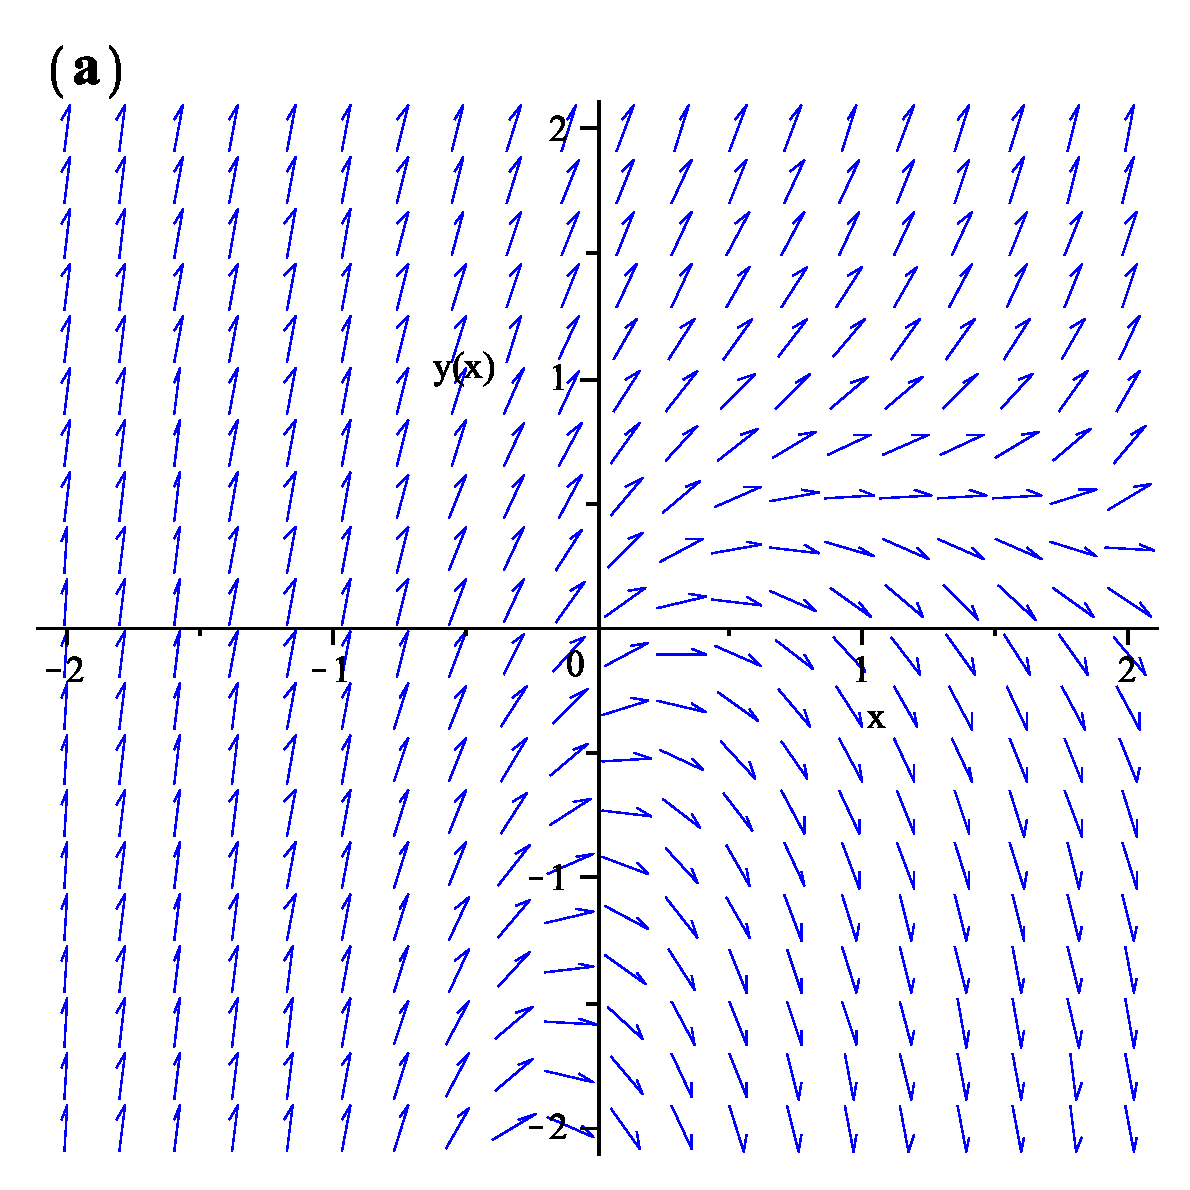
\includegraphics[width=2.0in]{VOLUMEN_2/02_Series/Figuras/Fig3a}
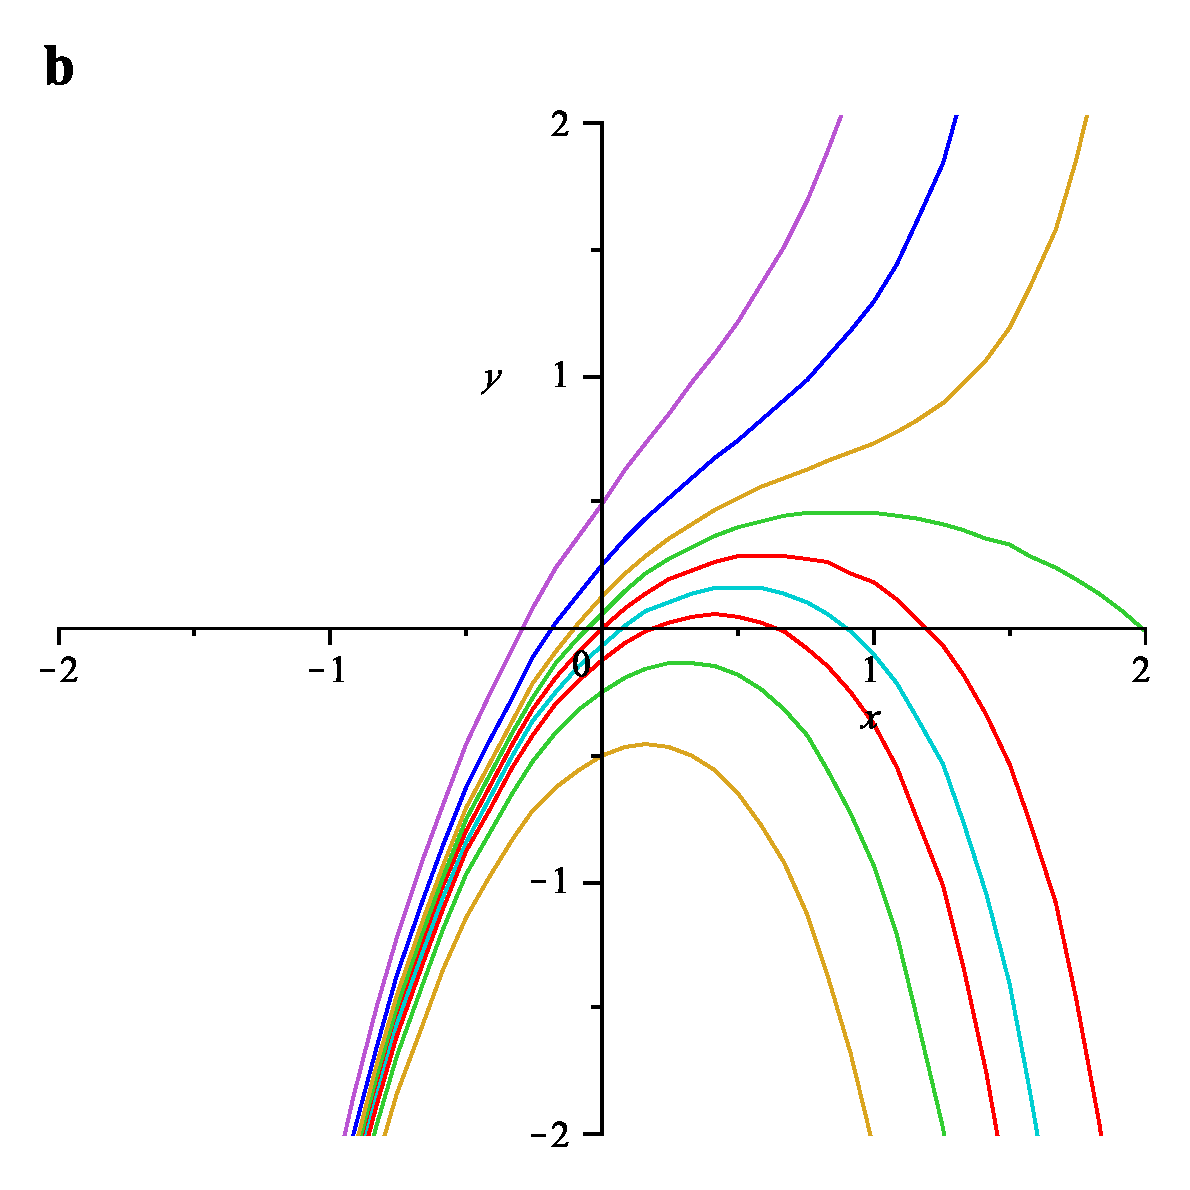
\includegraphics[width=2.0in]{VOLUMEN_2/02_Series/Figuras/Fig3b}
\includegraphics[width=2.0in]{VOLUMEN_2/02_Series/Figuras/Fig3c}
\caption{\small (a) Representaci�n de los campos vectoriales. (b) Diferentes soluciones para la  ecuaci�n diferencial (\ref{ecuanewton}). (c) La soluci�n correcta correspondiente al  valor inicial $y(0)=0$  con las diferentes soluciones aproximadas.}
\label{curvasvectoriales}
\end{center}
\end{figure}

Comencemos entonces nuestro estudio sobre ecuaciones diferenciales precisamente con las series matem�ticas.

\subsection{Introducci�n a las sucesiones}

Para empezar, vayamos a la noci�n elemental de sucesiones. B�sicamente, una sucesi�n es una  colecci�n numerable de elementos, dados en cierto orden, como:
\[
1, 2, 3, 4, \, \dots \,, \quad 1, x, x^2, x^3,  \, \dots \,, \quad
a, b, c, d \,.
\]

En matem�ticas se puede entender las sucesiones como una aplicaci�n desde los n�meros naturales a cualquier otro conjunto, no necesariamente de la misma naturaleza. Estos n�meros se denominan los t�rminos, elementos o miembros de la sucesi�n. Siendo m�s rigurosos, una sucesi�n se puede definir como una funci�n sobre el conjunto de los n�meros naturales, es decir, que estar�amos hablando en este caso de una funci�n discreta.

Es bastante com�n que se confundan las sucesiones con series matem�ticas, veremos que una serie entenderemos es en realidad una suma de t�rminos.

Las sucesiones se diferencian de los conjuntos en el hecho de que es importante considerar el orden en que aparecen distribuidos.  Adem�s, un mismo t�rmino de una sucesi�n puede aparecer varias veces en posiciones diferentes. Esto significa que las siguientes sucesiones finitas son diferentes:
\[
a, b, c, d  \quad \neq \quad  b, c, d, a \,.
\]

Una sucesi�n puede contener infinitos elementos y en este caso se denomina una sucesi�n infinita, por lo tanto, si a cada n�mero entero positivo se le asocia un elemento $u_n$, entonces el conjunto ordenado: 
\[
u_1, u_2, u_3, . . . u_n, \, \dots \,. 
\]
define una sucesi�n infinita. Cada t�rmino $u_n$ tendr� un siguiente t�rmino $u_{n+1}$ y por lo tanto no existe un �ltimo t�rmino. 

Las sucesiones se pueden expresar de una manera m�s sencilla definiendo el $n$-�simo t�rmino, como por ejemplo: 
\[
u_n=\frac1n \,, \qquad n=1, 2, 3 , \dots
\]
cuyos primeros cuatro t�rminos son: 
\[
1, \frac12, \frac13, \frac14 \,. 
\]

Otra manera de definir sucesiones es por medio de una relaci�n de recurrencia, por ejemplo, para la bien conocida sucesi�n de Fibonacci la relaci�n de recurrencia es:
\[
u_1=u_2=1\,\,, \qquad u_{n+1}=u_n +u_{n-1} \,\,, \qquad n \geq 2\,, 
\]
y cuyos primeros t�rminos son: 
\[
1, 1, 2, 3, 5, 8, 13, 21, 34, \dots 
\]

Como curiosidad matem�tica, podemos ver que existe una funci�n que permite generar los n�meros de Fibonacci, esta funci�n cuando se expande en potencias de $x$ tiene como coeficientes, �los n�meros de Fibonacci!
\[
f(x)= \frac{x}{1-x-x^2}= x+{x}^{2}+2\,{x}^{3}+3\,{x}^{4}+5\,{x}^{5}+8\,{x}^{6}+13\,{x}^{7}+21
\,{x}^{8}+34\,{x}^{9} + \cdots
\]

Tambi�n es posible definir una sucesi�n a trav�s del concepto de funci�n. Se define una funci�n para los enteros positivos, de manera que $f(n)$ es el t�rmino $n$-�simo de la sucesi�n para cada $n=1, 2, 3, \dots$. Por lo tanto, los t�rminos de las sucesi�n se escriben como:
\[
f(1), f(2), f(3), . . . f(n), \dots
\]

Las siguientes f�rmulas son ejemplos de sucesiones:
\begin{eqnarray*}
f(n) &=& (-1)^n \,\, \Rightarrow \,\, -1, 1, -1, 1, -1, \dots \\
f(n)&=& \mbox{sen}\left(\frac{n\pi}{2}\right) \,\, \Rightarrow \,\, 
\sin \left( \frac{\pi}{2} \right), \sin \left( \pi \right), 
\sin \left( \frac{3\pi}{2}  \right), \sin \left( 2\,\pi \right),  
\sin \left( \frac{5 \pi}{2} \right)\dots \\
f(n)&=&(-1)^n\left[1+\frac1n \right] \,\, \Rightarrow \,\,
-2, \frac32,  -\frac43,  \frac54,  -\frac65 \dots
\end{eqnarray*}

Las sucesiones pueden tener la caracter�stica de ser crecientes o decrecientes. Una sucesi�n  $\{ f(n)\}$ se dice que es creciente si:
\[
f(n) \leq f(n+1) \quad \forall \quad n \geq 1 \,,
\]
es decir, cada t�rmino es menor o igual al t�rmino siguiente. Y si de impone la condici�n $f(n) < f(n+1)$ se denomina {\it estrictamente creciente}. Por otro lado, una sucesi�n se llama decreciente si:
\[
f(n) \geq f(n+1) \quad \forall \quad n \geq 1\,.
\]
y {\it estrictamente decreciente} si  $f(n) > f(n+1)$.

%%%%%%%%%%%%%%%%%
\begin{figure}[h]
\begin{minipage}{7.4cm}
Las sucesiones pueden estar acotadas de diferente manera. Diremos que la sucesi�n $\{ f(n)\}$ es acotada {\it superiormente}  si existe un n�mero positivo $M$ tal que $f(n)\leq M $ para todo $n$. Tambi�n puede ser acotada {\it inferiormente} si existe un n�mero positivo $N$ tal que $f(n)\geq N $ para todo $n$. En el caso de cumplirse ambas condiciones hablaremos de una sucesi�n acotada $N \leq f(n) \leq M$.

Podemos hablar de sucesiones mon�tonas cuando la diferencia entre un t�rmino y el que le sigue siempre es del mismo signo y adem�s son del tipo creciente o decreciente.

Nos vemos ahora en la necesidad de hablar del significado de los t�rminos convergencia o divergencia de una sucesi�n.
\end{minipage} \hfill 
\begin{minipage}{8.0cm} 
\includegraphics[width=3.0in]{VOLUMEN_2/02_Series/figuras/Converging.jpg}
\caption{Sucesi�n convergente a cero.}
\label{FigSerieConverge}
\end{minipage}
\end{figure}
%%%%%%%%%%%%%%%%%

La convergencia o divergencia se determina de manera sencilla, como lo indica el siguiente teorema:

\begin{mdframed}[linecolor=OliveGreen,linewidth=0.3mm]
\textbf{Teorema}: Una sucesi�n mon�tona converge si y s�lo si es acotada.
\end{mdframed}

Revisemos el concepto de convergencia (divergencia). Cuando una sucesi�n converge, lo que significa es que tiende a un valor particular llamado su l�mite, diremos en �ste caso la sucesi�n ser� una {\it sucesi�n convergente}. Las sucesiones que no son convergentes se denominan {\it divergentes}.

En otras palabras, una sucesi�n tiene l�mite si los elementos de la sucesi�n se hacen cada vez m�s y m�s cercanos a alg�n valor  $L$ (llamado l�mite de la sucesi�n). Esto  significa que dado un n�mero real $\varepsilon$  mayor que cero, todos menos un n�mero finito de elementos de la sucesi�n estar�n siempre a una distancia a $L$ menor que $\varepsilon$.

Matem�ticamente es lo siguiente: 
\begin{equation}
\lim_{n \rightarrow \infty } f(n)=L \,.
\label{limisuce}
\end{equation}

Si una sucesi�n $f(n)$ converge, entonces el l�mite \ref{limisuce}  existe, es �nico y la sucesi�n es acotada.

En la figura \ref{FigSerieConverge} podemos ver una representaci�n gr�fica para la sucesi�n:
\[
f(n)=\frac{n+1}{2n^2} \,.
\]
Esta serie converge, y es f�cil ver que:
\[
\lim_{n \rightarrow \infty } \frac{n+1}{2n^2}=0 \,.
\]

%%%%%%%%%%%%%%%%%
\begin{figure}[h]
\begin{minipage}{7.4cm}
Tambi�n existen las sucesiones oscilantes, las cuales suelen ser divergentes por no tener l�mite. Estas sucesiones presentan t�rminos que se alternan de manera indefinida. Cuando cambian de signo se llaman sucesiones alternadas, como la que mencionamos anteriormente $f(n) = (-1)^n \,\, \Rightarrow \,\, -1, 1, -1, 1, -1, \dots $.

Un ejemplo particular de sucesiones oscilantes convergentes es la {\it sucesi�n de Cauchy}. Una sucesi�n de n�meros reales: $x_1, x_2, x_3, \dots$ se denomina una sucesi�n de Cauchy fundamental si para todo n�mero positivo $\varepsilon$ existe un entero positivo $M$ tal que para todos los n�meros naturales $n, m > M$ se cumple:
\[
\left|x_m-x_n \right| <\varepsilon \,.
\]
\end{minipage} \hfill 
\begin{minipage}{8.0cm} 
\includegraphics[width=3.0in]{VOLUMEN_2/02_Series/figuras/Cauchy_sequence.jpg}
\caption{Sucesi�n de Cauchy.}
\label{FigSerieCauchy}
\end{minipage}
\end{figure}
%%%%%%%%%%%%%%%%%

En este tipo de sucesiones los elementos se la sucesi�n se vuelven arbitrariamente cercanos entre s� a medida que  la sucesi�n progresa, como se puede ver en la figura \ref{FigSerieCauchy}. Esta condici�n, necesaria para hablar de convergencia, se llama la condici�n de Cauchy. 

Existe una serie de resultados interesantes que podemos mencionar:
\begin{itemize}
\item Toda sucesi�n convergente es de Cauchy.
\item Toda sucesi�n de Cauchy est� acotada.
\item Para los n�meros reales $\mathds{R}$, toda sucesi�n de Cauchy es convergente.
\item Toda sucesi�n convergente est� acotada.
\end{itemize}


A medida que $n$ se hace cada m�s grande, el valor de una sucesi�n $\{f(n)\}$ o $\{u_n\}$ se puede comportar de una manera bastante particular. Por ejemplo, si $u_n=1/n$, es claro que $u_n$ {\it converge} a cero a medida que $n \rightarrow \infty$. Pero si $u_n=e^{\alpha n}$, el l�mite depender� del valor de $\alpha$. 

Por lo tanto, la pregunta a responder tiene que ver con el hecho de saber si los t�rminos de $u_n$ tienden, o no,  a un l�mite finito cuando $n$ crece indefinidamente.

\subsection{Acerc�ndonos al concepto de series}

Con el concepto de sucesiones es posible definir una expresi�n anal�tica que formalmente tiene aspecto de suma, que contiene un n�mero infinito de sumandos y que denominaremos {\it serie infinita}. 

Si $\{u_n\}$ (con $n=1, 2, 3, \dots$) es una sucesi�n infinita de n�meros reales o complejos, es posible formar una nueva sucesi�n $\{s_n\}$ a partir de tomar sumas parciales de $\{u_n\}$. Veamos el procedimiento:
\[
s_1=u_1\,,\quad 
s_2=u_1+u_2\,,\quad 
s_3=u_1+u_2+u_3\,, \quad  \dots \quad  
s_n=u_1+u_2+u_3+ \cdots u_n = \sum_{i=1}^n \, u_i\,.
\]

Es decir, partimos con $s_1=u_1$ y decimos que para todo $n \in \mathds{N}$ se tiene que $s_{n+1}=s_n+u_{n+1}$. La sucesi�n  $\{s_n\}$ la llamaremos la serie de t�rmino general $a_n$ definida a trav�s de la sucesi�n $\{u_n\}$ y la representaremos por:
\begin{equation}
\label{defserie}
\sum_{n=1}^{\infty} \, u_n \,.
\end{equation}
Al n�mero 
\[
s_n=\sum_{i=1}^{n} \, u_i \,
\]
le denominaremos la suma parcial de orden $n$ de la serie (\ref{defserie}).

Es importante aclarar que una serie es una sucesi�n cuyos t�rminos se obtienen al sumar de manera consecutiva lo t�rminos de una sucesi�n diferente. 

Si la sucesi�n $s_n$ tiende a un l�mite $S$, la serie infinita 
\[
\sum_{i=1}^\infty \, u_i \,,
\]
se dice que es convergente y converge al valor $S$, el cual es �nico. Entonces se puede escribir:
\begin{equation}
\label{def_serie}
S=u_1+u_2+u_3+\cdots + u_n + \cdots = \sum_{n=1}^\infty \, u_n =\lim_{n \rightarrow \infty} \{s_n\}= \lim_{n \rightarrow \infty} 
\sum_{i=1}^n \, u_i \,.
\end{equation}

El n�mero $S$ se denomina {\it la suma de la serie} infinita y debe ser entendido como el l�mite de la sucesi�n. 


Lo anterior se puede formalizar  diciendo que la condici�n para la existencia de un l�mite $S$ es que  para cada $\varepsilon > 0$ existe un n�mero $N=N(\varepsilon) \in \mathds{N}$ tal que:
\[
| S - s_{i} | < \varepsilon \quad \text{para} \ i > N 
\,\, \Rightarrow \,\,  
| s_{j}- s_{i} | < \varepsilon \quad \text{para, todo } \ i,j > N \,.
\]

Esta afirmaci�n se denomina \textbf{criterio de Cauchy}\footnote{{\bf Augustin Louis Cauchy} Par�s, 1789 - 1857, matem�tico franc�s pionero en los estudios de an�lisis (real y complejo) y de la teor�a de los grupos de permutaci�n. Cauchy hizo aportes importantes en los criterios de convergencia y divergencia de series infinitas, as� como tambi�n, en ecuaciones diferenciales, determinantes, probabilidades y f�sica matem�tica} sobre la convergencia de las series parciales, y viene a ser la condici�n necesaria y suficiente para que una suma parcial $s_{i}$ converja a medida que avanzamos en los t�rminos de la serie.

Se dir� que la serie \textit{diverge} si el valor de la sumatoria aumenta indeteniblemente.

La serie  tambi�n puede oscilar:
\[
s_{i}=\sum_{n=1}^{i} ( -1 )^{n}= 1-1+1-1+ \cdots + (-1 )^{i}+ \cdots 
\] 
Aqu� $s_n$ ser� $0$ o $1$ y por lo tanto el l�mite no existe.

La serie cuyos t�rminos son tomados a partir del $(n+1)$-�simo t�rmino, y en el mismo orden,  de la serie (\ref{def_serie}) se llama el {\it resto} $n$-�simo de la serie  (\ref{def_serie}) y se denota por:
\begin{equation}
\sum_{k=n+1}^{\infty} u_k \,\, \Rightarrow \,\, 
u_{n+1} +  u_{n+2} +  u_{n+3} + \cdots \,.
\end{equation}

Si el resto $n$-�simo de la serie (\ref{def_serie}) converge, entonces su suma:
\begin{equation}
r_n= \sum_{k=n+1}^{\infty} u_k \,,
\end{equation}
se denomina el {\it resto de la serie}.

De las series nos interesa conocer cu�nto suman. Es decir, cu�l es el valor de $s_{i}$ para una serie finita donde $i = N$. Pero tambi�n estamos interesados en conocer cu�nto suma una serie infinita. 

\subsection{Series elementales}
Probablemente, de cursos anteriores  hemos conocido algunas series emblem�ticas, estudiemos aqu� algunas de estas series:

\begin{itemize}

\item {\bf Serie aritm�tica}

Seguramente con anterioridad  hemos o�do hablar de progresiones aritm�ticas. Ellas son, sencillamente series de la forma:
 \[
 s_{N}=\sum_{n=0}^{N-1} (a+nd)= a+(a+d)+(a+2d)+(a+3d)+(a+4d)+\cdots+  \left[a +(N-1)d \right]\,,
 \]
donde $a$ y $d$ son n�meros reales o complejos.
  
Al desarrollar la serie anterior en orden inverso y sumarla con la serie original obtemos:
  \[
 \begin{array}{rcccccc}
s_{N}= & a & +(a+d) & +(a+2d) & +(a+3d)  & +\cdots &+ \left[a +(N-1)d \right] \\
s_{N}= & \left[a +(N-1)d \right] & + \left[a +(N-2)d \right] & + \left[a +(N-3)d \right] & + \left[a +(N-4)d \right] & +\cdots &+ a
 \end{array} 
\]  
resultando:
\[
2 s_{N}={N}\left[a +a + (N-1) d \right] \,\, \Rightarrow \,\, 
s_{N}= \frac{N}{2}\left[\text{Primer T�rmino} + \text{�ltimo T�rmino} \right]
\] 
obviamente, si $N \rightarrow \infty$ la serie diverge.
 
\item {\bf Serie Geom�trica}

De �sta serie tambi�n sabemos que:
\[
s_{N}=\sum_{n=0}^{N}x^{n} = 1 +x +x^{2}+x^{3}+\cdots+x^{N} \,,
\]  
y si realizamos la resta $s_{N}-x s_{N}$, tenemos
 \begin{equation}
 \begin{array}{rllllll}
s_{N}= & 1 & +x & +x^{2} & +x^{3}  & +\cdots &+ x^{N} \\
xs_{N}= & x & + x^{2} & + x^{3} & +x^{4} &+ \cdots &+ x^{N+1}
 \end{array} \nonumber
\end{equation} 

Es inmediato comprobar que:
\[ 
(1-x)s_{N}=1-x^{N+1} \,\, \Rightarrow \,\,
s_{N}= \frac{1-x^{N+1}}{1-x}= \frac{1}{1-x}-\frac{x^{N+1}}{1-x}\,,
\]

Notemos que si $x\neq1$ podemos reescribir la serie anterior como:
\begin{equation}
\label{seriegeo}
\sum_{n=0}^{n}x^{n} = 1 +x +x^{2}+x^{3}+\cdots+x^{n}=
\frac{1}{1-x}-\frac{x^{n+1}}{1-x}
\end{equation}

Por lo tanto podemos ver que si $|x|<1$ tendremos que la suma ser�:
\begin{equation}
\label{seriegeo2}
\lim_{n \rightarrow \infty}\frac{x^{n+1}}{1-x}= 0  \,\, \Rightarrow \,\,
\lim_{n \rightarrow \infty} \sum_{n=0}^{n}x^{n} =
 \sum_{n=0}^{\infty}x^{n} =\frac{1}{1-x} \,.
\end{equation}
Por otro lado, la serie divergir� (u oscilar�) si $|x| \geqslant 1$.

\item {\bf Series Aritm�tico-geom�tricas}

Estas series, un poco m�s ex�ticas y como su nombre lo sugiere son una combinaci�n de las anteriores. 
  \[
 s_{N}= \sum_{n=0}^{N-1} (a+nd)x^{n}=
 a+(a+d)x+(a+2d)x^{2}+(a+3d)x^{3}+(a+4d)x^{4}+\cdots+  \left[a +(N-1)d \right]x^{N-1} \,.
  \] 
  
Utilizando la misma estrategia que aplicamos a las series  geom�tricas (se deja como ejercicio al lector) se llega a encontrar el valor, nada intuitiva,  de la suma $S$:
 \[
s_{N}=\frac{a -\left[ a + (N-1)d \right]x^{N}}{1-x} + 
\frac{ xd(1 -x^{N-1} )}{(1-x)^{2}}  \,. 
\] 

Otra vez,  si $|x|<1$,  entonces cuando $N \rightarrow \infty$ la serie converge a:
\[
S=\frac{a}{1-x} +\frac{xd}{(1-x)^{2}}\,.
\] 

\item {\bf Serie Arm�nica} 

Quiz� no la conoc�amos con este nombre (y menos por sus propiedades) pero  seguro nos la hemos tropezado. 
\[
\sum_{n=1}^{\infty} \frac{1}{n}=1+ \frac{1}{2} +\frac{1}{3} +\frac{1}{4} +\frac{1}{5} +\cdots\frac{1}{n} +\cdots 
\]

Esta serie infinita resulta ser enga�osa, en apariencia parece converger, pero no es as�. Adem�s notemos lo siguiente:
\[
\sum_{n=1}^{20} \frac{1}{n} \approx 3,5977\,, \quad 
\sum_{n=1}^{220} \frac{1}{n} \approx 5,9731\,, \quad
\sum_{n=1}^{20220} \frac{1}{n} \approx 10,492\,, 
\]
la suma de los primeros $20$ t�rminos es m�s grande que la suma de los siguientes !`$200$ t�rminos! y da la impresi�n de que la serie crece muy lentamente hacia alg�n valor l�mite.

Si analizamos con m�s cuidado, veremos que hay sutilezas. Acomodemos los t�rminos de la siguiente forma:
\[
\sum_{n=1}^{\infty} \frac{1}{n} = 1  + \underbrace{\frac{1}{2}}_{\sigma_{0}} 
+ \underbrace{ \left( \frac{1}{3} +\frac{1}{4} \right) }_{\sigma_{1}} 
+ \underbrace{\left( \frac{1}{5} +\frac{1}{6}  +\frac{1}{7}  +\frac{1}{8}   \right)}_{\sigma_{2}} 
+ \underbrace{\left( \frac{1}{9} +\frac{1}{10}  + \cdots  +\frac{1}{16}   \right)}_{\sigma_{3}} + \cdots 
\]
la expresi�n anterior puede ser reescrita como:
\[
\sum_{n=1}^{\infty} \frac{1}{n} =
1 
+  \underbrace{ \frac{1}{1+1} }_{\sigma_{0}} 
+  \underbrace{ \frac{1}{2+1} + \frac{1}{2+2}}_{\sigma_{1}} 
+  \underbrace{ \frac{1}{4+1} + \frac{1}{4+2} + \frac{1}{4+3} + \frac{1}{4+4}}_{\sigma_{2}}
\]
\[
+  \underbrace{ \frac{1}{8+1} + \frac{1}{8+2} + \cdots +\frac{1}{8+8} }_{\sigma_{3}} +\cdots
+ \sum_{j=1}^{2^{n}} \frac{1}{2^{n}+j} +\cdots
\]
con lo cual:
\[
\sigma_{0}=\frac{1}{2}; \quad 
\sigma_{1}=\frac{7}{12} > \frac{1}{2}; \quad 
\sigma_{2}= \frac{533}{840}> \frac{1}{2}; \quad 
\sigma_{3}=\frac{95549}{144144} >\frac{1}{2}; \cdots
\]
y claramente diverge ya que:
\[
1+ \sigma_{0} +\sigma_{1} +\sigma_{2} + \sigma_{3} +\cdots > 1 +\frac{1}{2}  +\frac{1}{2}  +\frac{1}{2}  +\frac{1}{2} +\cdots
\]
Esta prueba aparentemente se le debe a Nicole D'Oresme\footnote{\textbf{Nicole D'Oresme} (1323-1382) Matem�tico franc�s que invent� la geometr�a coordenada antes de Descartes. Sobre la serie arm�nica consulte: \url{http://mathworld.wolfram.com/HarmonicSeries.html}}. 

Ahora bien, notemos que para todo $n\in \mathds{N}$ resulta:

\begin{eqnarray*}
\int_{1}^n \frac{\mathrm{d}x}{x} = \ln(n) \,\, \Rightarrow \,\,
\ln(n) &=& \int_{1}^2 \frac{\mathrm{d}x}{x} + \int_{2}^3 \frac{\mathrm{d}x}{x} +\int_{3}^4 \frac{\mathrm{d}x}{x} +\cdots +
\int_{k}^{k+1}\frac{\mathrm{d}x}{x} =
\sum_{k=1}^{n-1}\ \int_{k}^{k+1}\frac{\mathrm{d}x}{x} \\
&\leq& \sum_{k=1}^{n-1}\ \int_{k}^{k+1}\frac{\mathrm{d}x}{k} <
1+\frac12+\frac13+\cdots +\frac{1}{n} \,.
\end{eqnarray*}

Es decir
\[
\lim_{n \rightarrow \infty} \left[1+\frac12+\frac13+\cdots +\frac{1}{n} \right] \geq \lim_{n \rightarrow \infty} \ln(n) = + \infty \,.
\]
Por lo tanto:
\[
\sum_{n=1}^{\infty} \frac{1}{n} = +\infty \,.
\]


Una de las generalizaciones de la serie arm�nica es la funci�n Zeta de Riemann\footnote{\textbf{Georg Friedrich Bernhard Riemann} (1826 Hanover, Alemania - 1866 Selasca, Italia) Matem�tico alem�n cuyas ideas sobre las geometr�a del espacio han tenido un profundo impacto en el desarrollo de la f�sica te�rica. Igualmente clarific� la noci�n de integral al introducir el concepto de lo que hoy se conoce como \textit{integral de Riemann}.  M�s detalles en  \url{http://mathworld.wolfram.com/RiemannIntegral.html}.}
\[
 \zeta(z) = \sum_{n=1}^{\infty} \frac{1}{n^z} =
 \frac{1}{1^z}+\frac{1}{2^z}+\frac{1}{3^z}+\cdots 
 \,,\quad \Re(z)>1 \,.
 \]
 
Esta �ltima expresi�n es tambi�n un ejemplo donde  a partir de una serie se define una funci�n, en este caso una funci�n anal�tica. Aqu� $z$ puede ser un n�mero complejo, $z=a+ib$, y la serie converge cuando su parte real es mayor o igual a 1. 

La funci�n Zeta de Riemann viene tambi�n definida por:
\[
 \zeta(z) = \frac{1}{\Gamma(z)}\int_0^\infty 
 \frac{x^z}{x\left(e^x-1\right)} \mathrm{d}x \,, \,\, \mbox{ donde }\,\,
 \Gamma(z)=\int_0^\infty \frac{x^z e^{-x}}{x} \mathrm{d}x \,,
\]
$\Gamma(z)$ es la funci�n gamma. 


\end{itemize}

Las mayor�a de las series que hemos mencionado con anterioridad tienen la particularidad de que todos sus t�rminos son positivos, es decir, para la serie $\sum  a_n$ se tiene que $a_n \geq 0$, y por lo tanto:
\[
s_n = s_{n-1} + a_n \geq s_{n-1}\,,
\]
de manera que las sumas parciales $s_n$ son una sucesi�n mon�tona creciente.


\subsection{Derivaci�n de  series geom�tricas elementales}

Las series infinitas se encuentran entre las m�s poderosas herramientas que se introducen en un curso de c�lculo elemental. Son un ejercicio bastante inteligente para la manipulaci�n de limites y son una buena herramienta para el estudio de las ecuaciones diferenciales, en el desarrollo de m�todos num�ricos y para estimar el comportamiento de funciones. 

Consideremos la serie geom�trica: 
\[
a+ az+ az^2 +az^3 +\cdots +az^n+ \cdots \] con $|z|<1$. Este es 
uno de los pocos ejemplos donde se puede encontrar el t�rmino de las sumas parciales  a trav�s de una expresi�n sencilla. Esta serie se puede tomar como punto de partida para encontrar la suma de un gran n�mero de series interesantes. Consideremos el caso $a=1$ y $z=x$, como en la ecuaci�n (\ref{seriegeo2}).
\begin{equation}
\label{seriegeom}
1+ x+ x^2 +x^3 +\cdots +x^n+ \cdots = \frac{1}{1-x} \,,\,\,\,\, |x| < 1\,.
\end{equation}

Si cambiamos $x$ por $x^2$ en (\ref{seriegeom}) resulta:
\begin{equation}
\label{seriegeom2}
1+ x^2+ x^4 +x^6 +\cdots +x^{2n}+ \cdots = \frac{1}{1-x^2} \,,\,\,\,\, |x| < 1\,.
\end{equation}

Si se multiplica (\ref{seriegeom2}) por $x$ se obtiene:
\begin{equation}
\label{seriegeom3}
x+ x^3+ x^5 +x^7 +\cdots +x^{2n+1}+ \cdots = \frac{x}{1-x^2} \,,\,\,\,\, |x| < 1\,.
\end{equation}

Si cambiamos $x$ por $-x$ en (\ref{seriegeom}) resulta:
\begin{equation}
\label{seriegeom4}
1- x+ x^2 -x^3 +\cdots +(-1)^nx^{n}+ \cdots = \frac{1}{1+x} \,,\,\,\,\, |x| < 1\,.
\end{equation}

Si cambiamos $x$ por $x^2$ en (\ref{seriegeom4}) resulta:
\begin{equation}
\label{seriegeom5}
1- x^2+ x^4 -x^6 +\cdots +(-1)^nx^{2n}+ \cdots = \frac{1}{1+x^2} \,,\,\,\,\, |x| < 1\,.
\end{equation}

Si se multiplica (\ref{seriegeom5}) por $x$ se obtiene:
\begin{equation}
\label{seriegeom6}
x- x^3+ x^5 -x^7 +\cdots +(-1)^nx^{2n+1}+ \cdots = \frac{x}{1+x^2} \,,\,\,\,\, |x| < 1\,.
\end{equation}

Si cambiamos $x$ por $2x$ en (\ref{seriegeom2}) resulta:
\begin{equation}
\label{seriegeom7}
1+4x^2+16x^4+\cdots + 4^nx^{2n}+ \cdots=\frac{1}{1-4x^2} \,,\,\,\,\, |x| < \frac12 \,.
\end{equation}

Si se deriva (\ref{seriegeom}) entonces:
\begin{equation}
\label{seriegeom8}
1+2x+3x^2+\cdots + nx^{n-1}+ \cdots=\frac{1}{(1-x)^2} \,,\,\,\,\, |x| < 1 \,.
\end{equation}

Si se integra (\ref{seriegeom4}):
\begin{equation}
\label{seriegeom9}
x-\frac{x^2}{2}+\frac{x^3}{3}-\frac{x^4}{4}+\cdots + \frac{(-1)^nx^{n+1}}{n+1}+ \cdots=\ln(1+x) \,,\,\,\,\, |x| < 1 \,.
\end{equation}

Si se integra (\ref{seriegeom5}) ahora resulta:
\begin{equation}
\label{seriegeom10}
x-\frac{x^3}{3}+\frac{x^5}{5}-\frac{x^7}{7}+\cdots + \frac{(-1)^nx^{2n+1}}{2n+1}+ \cdots=\arctan(x) \,,\,\,\,\, |x| < 1 \,.
\end{equation}

Siguiendo a Laplace, quien dijo que hab�a que leer a Euler: ``{\it Read Euler, read Euler. He is the master of us all} ",  podemos hacer lo siguiente con  la serie (\ref{seriegeom9}):
\begin{equation}
\label{seriegeom9a}
\ln(1+x) = x-\frac{x^2}{2}+\frac{x^3}{3}-\frac{x^4}{4}+\cdots  
\end{equation}

Es bueno acotar que Euler utiliz� esta expresi�n para construir 
�tablas de logaritmos! 

Ahora hagamos lo siguiente, cambiemos $x$ por $-x$ en la ecuaci�n anterior:
\begin{equation}
\label{seriegeom9b}
\ln(1-x) = -x-\frac{x^2}{2}-\frac{x^3}{3}-\frac{x^4}{4}-\cdots 
\end{equation}
restando (\ref{seriegeom9a}) menos (\ref{seriegeom9b}):
\begin{eqnarray*}
\label{seriegeom9c}
\ln(1+x)-\ln(1-x) &=& \left[x-\frac{x^2}{2}+\frac{x^3}{3}-\frac{x^4}{4}+\cdots \right]  - 
\left[ -x-\frac{x^2}{2}-\frac{x^3}{3}-\frac{x^4}{4}-\cdots \right] \\
&=& 2x +\frac{2x^3}{3}+\frac{2x^5}{5}+\cdots
\end{eqnarray*}

Es decir:
\[
\label{seriegeom9d}
\ln \left( \frac{1+x}{1-x} \right)= 2x +\frac{2x^3}{3}+\frac{2x^5}{5}+\cdots
\]

Para valores peque�os de $x$, digamos $x=1/3$ resulta:
\[
\ln \left( \frac{1+\frac{1}{3}}{1-\frac{1}{3} } \right)=\ln \left( 2\right) = 
2\left(\frac{1}{3}\right) +\frac{2\left({\frac{1}{3}}\right)^3}{3}+\frac{2\left({\frac{1}{3}}\right)^5}{5}+\cdots
\approx 0.6930041152
\]

Euler not� la siguiente conexi�n entre logaritmos y las series arm�nicas. Cambiando $x$ por $1/n$ en (\ref{seriegeom9a}) se obtiene
\[
\label{seriearmo}
\ln \left(1+\frac{1}{n}\right) = \frac{1}{n}-\frac{1}{2n^2}+\frac{1}{3n^3}-\frac{1}{4n^4}+\cdots  
\]
por lo tanto:
\[
\label{seriearmo1}
 \frac{1}{n} = \ln \left(1+\frac{1}{n}\right) +\frac{1}{2n^2}-\frac{1}{3n^3}+\frac{1}{4n^4}-\cdots  
\]
y para valores de $n$ muy grandes, se cumple que:
\[
 \frac{1}{n} = \ln \left(\frac{n+1}{n}\right) 
\]

Ahora bien, para diferentes valores de $n$  se obtienen las siguientes relaciones
\begin{eqnarray*}
n=1 \,\, \Rightarrow \,\,1 &=& \ln \left(2\right) +\frac{1}{2}-\frac{1}{3}+\frac{1}{4}-\cdots \\
n=2 \,\, \Rightarrow \,\, \frac{1}{2} &=&  \ln \left(\frac{3}{2}\right) +\frac{1}{8}-\frac{1}{24}+\frac{1}{64}-\cdots \\
n=3 \,\, \Rightarrow \,\, \frac{1}{3} &=&  \ln \left(\frac{4}{3}\right) +\frac{1}{18}-\frac{1}{81}+\frac{1}{324}-\cdots \\
  \vdots & & \qquad  \vdots   \qquad \quad \vdots  \qquad  \vdots   \qquad \vdots \\
 \frac{1}{n} &=& \ln \left(\frac{n+1}{n}\right) +\frac{1}{2n^2}-\frac{1}{3n^3}+\frac{1}{4n^4}-\cdots  
\end{eqnarray*}

Si sumamos  columna por columna  resulta:
\begin{eqnarray*}
\sum_{k=1}^{n} \frac{1}{k} &=& \ln \left(2\right) +\ln \left(\frac{3}{2}\right)+ \ln \left(\frac{4}{3}\right) + \cdots +
 \ln \left(\frac{n+1}{n}\right)\\
 &+& \frac{1}{2}\left[  1 +  \frac{1}{4} + \frac{1}{9} + \cdots +  \frac{1}{n^2} \right] 
 - \frac{1}{3}\left[  1 +  \frac{1}{8} + \frac{1}{27} + \cdots +  \frac{1}{n^3} \right] \\
  &+& \frac{1}{4}\left[  1 +  \frac{1}{16} + \frac{1}{81} + \cdots +  \frac{1}{n^4} \right]   - \cdots
\end{eqnarray*}

Es f�cil ver que la suma de los logaritmos de la primera l�nea se puede escribir  como el logaritmo de sus productos, es decir, 
\[
\ln \left(2\right) +\ln \left(\frac{3}{2}\right)+ \ln \left(\frac{4}{3}\right) + \cdots + \ln \left(\frac{n+1}{n}\right) = 
\ln \left[ 2 \left(\frac{3}{2}\right)  \left(\frac{4}{3}\right)\cdots   \frac{n+1}{n} \right]  = \ln \left(n+1\right) \,.
\]

De manera que, y siguiendo a Euler que llev� a cabo un estimado para los t�rminos sobrantes, resulta lo siguiente:
\[
\sum_{k=1}^{n} \frac{1}{k}  \approx  \ln \left(n+1\right) + 0.577218 \,.
\]

Para valores de $n$ muy grandes la suma de las serie arm�nica es igual a un logaritmo m�s una constante. Esta
constante es actualmente llamada la Constante de Euler y denotada por la letra $\gamma$:
\begin{equation}
\gamma = \lim_{n \rightarrow \infty} \left[ \sum_{k=1}^{n} \frac{1}{k}  -  \ln \left(n+1\right) \right] \,.
\end{equation}

La constante de Euler  juega un papel central en otras ramas de las matem�ticas, por ejemplo, en el an�lisis real aparece como:
\[
\gamma = - \int_{0}^{\infty} e^{-x}  \ln \left(x\right) \textrm{d}x \,.
\]

\subsection{El m�todo de la diferencia}

A veces para una serie finita, $\{s_{N}\}$, uno encuentra que para el t�rmino $n$-�simo se tiene que: 
\[
a_{n}= f(n) -f(n-1) \,.
\] 
para alguna funci�n $f(n)$. 

En ese caso es inmediato demostrar lo siguiente:
\begin{equation}
s_{N}=\sum_{n=1}^{N}a_{n}=\sum_{n=1}^{N} f(n) - \sum_{n=1}^{N} f(n-1)= 
f(N) -f(0) \,.
\label{sumadiferencia}
\end{equation} 
Por ejemplo, si tenemos la serie:
\[
\sum_{n=1}^{N} \frac{1}{n(n+1)}\,,
\] 
se puede ver que:	
\[
a_{n}=\frac{1}{n(n+1)}  = - \frac{1}{n+1} +\frac{1}{n}  
\,\, \Rightarrow \,\,  f(n)= -\frac{1}{n+1} \,,
\] 	
por lo tanto, la suma se podr� expresar como: 
\[
s_{N}= f(N)-f(0)= -\frac{1}{N + 1} +1=\frac{N}{N + 1} \,.
\]

Se puede ir m�s all� si identificamos que el t�rmino $n$-�simo tiene la forma: 
\[
a_{n}= f(n) -f(n-m)\,,
\] 
por lo tanto,  la suma de la serie se puede escribir como:
\begin{equation}
s_{N}=\sum_{n=1}^{N}a_{n}=\sum_{n=1}^{N} f(n) - \sum_{n=1}^{N} f(n-m) \,.
\label{sumadiferencia2}
\end{equation} 

Hay que hacer notar que el argumento $n-m$ puede ser positivo o negativo. Con lo cual el m�todo de la diferencia resulta vers�til y muy �til cuando se requiere encontrar la suma de series de variada dificultad. Podemos ver que:
\begin{itemize}
\item Si $m=1$
\[
s_{N}=\sum_{n=1}^{N}a_{n}=  f(N) -f(0) \,.
\]
como la ecuaci�n (\ref{sumadiferencia}).
\item Si $m=2$
\[
s_{N}=\sum_{n=1}^{N}a_{n}=  f(N) +f(N-1)-f(0)-f(-1) \,.
\]
\item Si $m=3$
\[
s_{N}=\sum_{n=1}^{N}a_{n}=  f(N) +f(N-1)+f(N-2) -f(0)-f(-1)-f(-2) \,.
\]
\end{itemize}

Consideremos la siguiente serie y su expansi�n en fracciones simples
 \[
\sum_{n=1}^{N} \frac{1}{n(n+2)} \,,
  \] 
se tiene que el t�rmino $n$-�simo es:
\[
 a_{n}=\frac{1}{n(n+2)}  = - \frac{1}{2(n+2)} +\frac{1}{2n} 
\,\, \Rightarrow \,\, f(n)= -\frac{1}{2(n+2)} \,,
 \]  
 de manera que:
 \[
 a_n=f(n)-f(n-2)=- \frac{1}{2(n+2)} -\left(-\frac{1}{2n} \right)\,,
 \]
de forma y manera que, como $m=2$, resulta:
\[
s_{N}= f(N) + f(N-1) - f(0) - f(-1) = 
\frac{3}{4} - \frac{1}{2} \left( \frac{1}{N + 2} + \frac{1}{N+1} \right)= 
{{N\,\left(3\,N+5\right)}\over{4\,\left(N+1\right)\,\left(N+2\right)}} \,.
\]

Ahora bien, con alguna frecuencia surgen las series de n�meros naturales. La m�s simple es: 
\[
s_{N}= 1+2+3+\cdots+N=\sum_{n=1}^{N}n=\frac{N(N+1)}{2} \,,
\]
es decir, una serie aritm�tica de raz�n $d=1$.

M�s interesante puede ser la serie de cuadrados de n�meros enteros:
\[
s_{N}= 1+2^{2}+3^{2}+\cdots+N^{2}=\sum_{n=1}^{N}n^{2}= \frac{N(N+1)(2N+1)}{6} \,.
\]

Este resultado, nada intuitivo, surge de la aplicaci�n ingeniosa del m�todo de la diferencia. Tal y como hemos dicho, se trata de encontrar que el elemento gen�rico de la serie sea: $a_{n}= f(n) -f(n-1)=n^{2}$ para alguna funci�n. 

Suponga una funci�n del tipo
\[
f(n)=n(n+1)(2n+1) \,\, \Rightarrow \,\, f(n-1)=(n-1)n(2n-1)\,,
\]
entonces:
\[
f(n) -f(n-1)= n(n+1)(2n+1) -  (n-1)n(2n-1) = 6n^{2}\,,
\]
con lo cual:
\[
a_{n}= 6 n^{2}\,\, \Rightarrow \,\,
s_{N} =\sum_{n=1}^{N}a_{n}=\frac{f(N) -f(0)}{6} = \frac{N(N+1)(2N+1)}{6}\,.
\]

\subsubsection{Sumando por analog�a}

Como siempre, intentaremos proceder por analog�a. La intenci�n es expresar una serie complicada como sumas de series conocidas. Considere el siguiente ejemplo:
\[
s_{N} = \sum_{n=1}^{N}(n+1)(n+3) = \sum_{n=1}^{N}\left(n^2+4n+3\right)=\sum_{n=1}^{N}n^2 +\sum_{n=1}^{N}4n +\sum_{n=1}^{N}3 \,,
\] 
con lo cual:
\[
s_{N}= \frac{N(N+1)(2N+1)}{6}  + \frac{N(N+1)}{2}  + 3N  = \frac{N(2N^{2} +15N +31)}{6}\,.
\]

\subsection{Algebra elemental de series}

\label{AlgebraElementalSeries}
Las series se suman, se igualan y se multiplican. Para ello es importante que tengamos cuidado con los �ndices y sus valores. Consideremos un par de series infinitas:
\[
u=\sum_{n=0}^{\infty}a_{n} \quad  \text{y} \quad v=\sum_{n=0}^{\infty}b_{n} \,,
\]
con lo cual la suma de esas series ser�:
\[
u + v = \sum_{n=0}^{\infty}a_{n} + \sum_{n=0}^{\infty}b_{n} = \sum_{n=0}^{\infty}\left(  a_{n}+b_{n}\right) \,. 
\] 
Los �ndices son mudos y se acomodan para ser sumados. 

Para sumar series es imperioso que los �ndices de cada serie comiencen con el mismo valor, esto es:
\[
\sum_{n=0}^{\infty}a_{n} + \sum_{j=1}^{\infty}b_{j} = \sum_{n=1}^{\infty}\left(  a_{n-1}+b_{n}\right) = a_{0} + \sum_{n=1}^{\infty}\left(  a_{n}+b_{n}\right) \,.
\]
N�tese que hemos hecho los siguientes cambios: $j\rightarrow n$ y  $n\rightarrow n-1$.

Algo parecido ocurre cuando las series se igualan:
\[
\sum_{n=0}^{\infty}b_{n}  =\sum_{n=1}^{\infty}na_{n} 
\,\, \Rightarrow \,\,
\sum_{n=0}^{\infty}b_{n} = \sum_{k=0}^{\infty} (k+1)a_{k+1}
\,\, \Longleftrightarrow \,\,
\sum_{n=0}^{\infty}\left[ (n+1)a_{n+1}-b_{n}\right] =0 \,.
\]

Para finalizar se puede comprobar que las series  tambi�n se pueden multiplicar:
\[
u\, v =  \sum_{n=0}^{\infty}a_{n}  \, \sum_{n=0}^{\infty}b_{n}   = \sum_{n=0}^{\infty}c_{n} \,,
\]
donde:
\[
c_{n}=a_{0}b_{n}+a_{1}b_{n-1}+\cdots+a_{j}b_{n-j}+\cdots
+a_{n-2}b_{2}+a_{n-1}b_{1}+a_{n}b_{0}\,.
\]

Cuando las sucesiones comprenden sumas y productos de otras sucesiones, es decir, s� 
$u_k$ y $v_k$ son dos sucesiones con $u_k \rightarrow U$ y  $v_k \rightarrow V$ cuando
$k \rightarrow \infty$, entonces se cumple que:
\begin{enumerate}
\item si $a$ y $b$ son n�meros independientes de $k$, entonces $au_k + bv_k \rightarrow aU+bV$ cuando $k \rightarrow \infty$.
\item $u_k v_k \rightarrow U V$ para $k \rightarrow \infty$.
\item si $V\neq 0$ entonces $u_k/v_k \rightarrow U/V$ a medida que  $k \rightarrow \infty$.
\item si $u_k< v_k$ $\forall$ $k>N$ entonces $U \leq V$ cuando $k \rightarrow \infty$.
\end{enumerate}

\begin{mdframed}[linecolor=OliveGreen,linewidth=0.3mm]
\textbf{Teorema}: Si la serie  $\sum_{n=1}^{\infty} u_{n} $ converge, entonces cualquiera de sus restos converge. Si cualquier resto de la serie $\sum_{n=1}^{\infty} u_{n} $ converge, entonces la propia serie tambi�n converge, y si  adem�s:
\[
S= \sum_{n=1}^{\infty} u_n \,,\quad  s_i= \sum_{n=1}^{\infty} u_n\,, 
\quad  r_i= \sum_{n=i+1}^{\infty} u_n\,.
\]
Entonces:
\[
S=s_i+r_i \,.
\]
\end{mdframed}

Se tiene entonces que es posible agregar o quitar un n�mero finito de t�rminos a la serie dada y esta operaci�n no influir� sobre su convergencia. Tambi�n se desprende del teorema anterior que si la serie converge entonces su resto tiende a cero:
\[
\lim_{i \rightarrow \infty} r_i = 
\lim_{i \rightarrow \infty} \left(S-s_i \right) =0 \,.
\]


\subsection{Series telesc�picas}

Una propiedad importante de las series finitas es la propiedad denominada telesc�pica:
\begin{equation}
\sum_{k=1}^{n}\left(a_k - a_{k+1} \right)= a_1 - a_{n+1}\,,
\end{equation}
para el caso de series infinitas, se consideran aquellas series $\sum u_n$ donde cada t�rmino
se puede expresar como una diferencia de la forma:
\[
u_n= a_n - a_{n+1}\,.
\]

Las series telesc�pica son series cuyas sumas parciales se van cancelando de manera tal que al final resulta un n�mero fijo de t�rminos:
\[(a_{1}-a_{2})+(a_{2}-a_{3})+(a_{3}-a_{4})+\cdots +(a_{n}-a_{n+1})=a_1-a_{n+1} \,.
\]

\begin{mdframed}[linecolor=OliveGreen,linewidth=0.3mm]
\textbf{Teorema}: Sean $\{u_n \}$ y $\{a_n \}$ dos sucesiones de n�meros reales o complejos tales que:
\[
u_n= a_n - a_{n+1} \quad \mbox{para} \quad n=1,2,3, . . . \,.
\]
Entonces la serie $\sum u_n$ converge si y s�lo si la sucesi�n $\{a_n \}$ converge, en cuyo caso se tiene:
\[
\sum_{n=1}^{\infty} u_n= a_1 - L \quad \mbox{donde} \quad L= \lim_{n \rightarrow \infty} a_n\,.
\]
\end{mdframed}

Consideremos la siguiente serie:
\[
\sum_{n=1}^{\infty} \frac{1}{n^2+n}\,.
\]
Podemos demostrar que:
\[
u_n= \frac{1}{n^2+n}=\frac1n -\frac{1}{n+1} \,,
\]
Es f�cil verificar que:
\[
\sum_{n=1}^{N} \left[\frac1n -\frac{1}{n+1}\right]=
\left[1-\frac12\right] + \left[\frac12-\frac13\right]+
\left[\frac13-\frac14\right] + \left[\frac14-\frac15\right]+ \cdots +
\left[\frac{1}{N}-\frac{1}{N+1}\right] = 1-  \frac{1}{N+1} \,.
\]

Pero si aplicamos el teorema anterior, tenemos entonces que: $a_n=1/n$ , $a_1=1$ y adem�s ya vimos que la sucesi�n $a_n=1/n$ converge:
\[
L= \lim_{n \rightarrow \infty} a_n =  
\lim_{n \rightarrow \infty} \frac1n = 0\,.
\]

Por lo tanto:
\[
\sum_{n=1}^{\infty} \frac{1}{n^2+n} = 1\,.
\]

Las series pueden llegar a tener comportamientos extra�os, como se ve con la siguiente serie arm�nica alternada:
\[
\sum_{n=1}^{\infty} \frac{(-1)^{(n-1)}}{n}= 1-\frac12 + \frac13 - \frac14 + \frac15 - \frac16 +\cdots \,, 
\]

Recordemos  que anteriormente estudiamos la serie geom�trica (\ref{seriegeo}), la cual volveremos a escribir pero est� vez intercambiando $x\rightarrow -x$, de manera que nos queda de la siguiente forma:
\begin{equation}
\label{seriegeom4b}
1- x+ x^2 -x^3 +\cdots +(-1)^nx^{n}+ (-1)^{n+1}\frac{x^{n+1}}{1+x} = \frac{1}{1+x} \,.
\end{equation}
Ecuaci�n que es v�lida para todo $n \in \mathds{N}$ y $x\neq 1$.

Integrando (\ref{seriegeom4b}) entre $0$ y $1$ se obtiene:
\begin{eqnarray*}
1- \frac12+ \frac13 -\frac14 +\cdots +(-1)^n\frac{1}{n+1}+ (-1)^{n+1}\int_{0}^{1}\frac{x^{n+1}}{1+x}\mathrm{d}x &=& \ln(2) \\
\sum_{k=1}^{n+1} \frac{(-1)^{(k-1)}}{k}+ 
(-1)^{n+1}\int_{0}^{1}\frac{x^{n+1}}{1+x}\mathrm{d}x  &=& \ln(2) \,.
\end{eqnarray*}

Por lo tanto:
\[
\ln(2)-\sum_{k=1}^{n+1} \frac{(-1)^{(k-1)}}{k}= 
(-1)^{n+1}\int_{0}^{1}\frac{x^{n+1}}{1+x}\mathrm{d}x \,.
\]

Se puede ver tambi�n que:
\[
\int_{0}^{1}\frac{x^{n+1}}{1+x}\mathrm{d}x \leq 
\int_{0}^{1}{x^{n+1}}\mathrm{d}x = \frac{1}{n+2}
\,\, \Rightarrow \,\, 
\ln(2)-\sum_{k=1}^{n+1} \frac{(-1)^{(k-1)}}{k}=\frac{1}{n+2}
\]
Entonces:
\[
\lim_{n \rightarrow \infty}
\left[ \ln(2)-\sum_{k=1}^{n+1} \frac{(-1)^{(k-1)}}{k} \right]=0
 \,\, \Rightarrow \,\, 
\ln(2)=\sum_{n=1}^{\infty} \frac{(-1)^{(n-1)}}{n}\,.
\]

La suma tienen el valor de $S=\ln(2)$. 


Se puede mostrar lo que sucede si se arreglan los  t�rminos de la manera siguiente:
\[
S= 1+\left(\frac13 - \frac12 + \frac15 \right) + \left(\frac17 - \frac14 + \frac19 \right)  
+ \left(\frac{1}{11} - \frac16 + \frac{1}{13} \right) + \cdots \,,
\]
la cual contiene exactamente los mismos t�rminos, aunque en orden diferente, pero ahora la serie converge a $S=\frac32 \ln(2)$. Esta aparente contradicci�n surge cuando  pasamos por alto el hecho de que al sumar los t�rminos de una serie no se hace la suma con los infinitos t�rminos, lo que hacemos es calcular un l�mite de una sucesi�n de t�rminos que se obtienen sumando de manera consecutiva los t�rminos de otra sucesi�n dada, es decir,  lo que se hacemos es aplicar un proceso de l�mite. 
Para que al sumar no importe el orden de los sumandos tendr�amos que sumar los infinitos t�rminos de la sucesi�n. 

A pesar de que  las series pueden presentar estos comportamientos extra�os, las series  resultan muy buenas representaciones aproximadas de funciones, por ejemplo:
\begin{equation}
e^x= 1 + x + \frac{x^2}{2!} + \frac{x^3}{3!} + \frac{x^4}{4!} + \cdots = 
\sum_{n=0}^{\infty} \frac{x^n}{n!}\,.
\end{equation}

La suma directa de una serie infinita no es un m�todo pr�ctico para estudiar su convergencia, por ejemplo, la serie
\[
\sum_{k=2}^{\infty} \frac{\ln(k)}{k^2} \,,
\]
converge al valor $0,937548. . . $, pero para obtener estos primeros cinco decimales se tendr�a que sumar unos $10^7$ t�rminos! 



Es necesario entonces desarrollar algunos criterios que nos permitan saber si una serie puede llegar a converger o no.

\subsection{{\color{Fuchsia}Ejemplos}}

\begin{enumerate}
\item Dada la sucesi�n $\{u_n\}$ de n�meros reales, se llama sucesi�n de Cauchy o sucesi�n fundamental, en el caso de que satisfaga el requisito siguiente: dado un n�mero real $r$ positivo se pueda conseguir dos enteros positivos $p$ y  $q$ tal que de $p > n_0$ y $q > n_0$ se deduzca que $|c_p - c_q| < r$?.

En los n�meros reales toda sucesi�n de Cauchy converge a alg�n l�mite. Esta particularidad implica un resultado importante en el an�lisis real que es la caracterizaci�n de Cauchy para la convergencia de sucesiones:

Una sucesi�n de n�meros reales es convergente (en los reales) si y solo si es de Cauchy.

\item Demuestre que
\[
\sum_{n=1}^{\infty}\frac{1}{2^n}= 1
\]
Se tiene que
\[
s_n=\frac12+\frac{1}{2^2}+\frac{1}{2^3}+\cdots + \frac{1}{2^n}\,,
\]
y que al multiplicar por $\frac12$ se obtiene
\[
\frac12s_n=\frac{1}{2^2}+\frac{1}{2^3}+\frac{1}{2^4}+\cdots + \frac{1}{2^{n+1}}\,,
\]
restando
\[
\left[1-\frac12\right] s_n=\frac{1}{2}-\frac{1}{2^{n+1}} = 1- \frac{1}{2^n}\,.
\]
por lo tanto
\[
\lim_{n\rightarrow \infty} \left[1- \frac{1}{2^n}\right] =1\,,
\]
la serie converge.


\end{enumerate}

\subsection{{\color{red}Practicando con Maxima}} 

{\bf Maxima} puede calcular f�cilmente sumas num�ricas finitas, pero cuando le pedimos calcular sumas simb�licas infinitas podr� calcularlas solo en casos particulares.  Es �til al trabajar con series utilizar la librer�a  {\bf simplify\_sum}

Veamos algunos ejemplos sencillos de sumas

%%%%%% INPUT:
\begin{minipage}[t]{8ex}
{\color{red}\bf \begin{verbatim} (%i1) 
\end{verbatim}}
\end{minipage}
\begin{minipage}[t]{\textwidth}{\color{blue}
\begin{verbatim}
load(simplify_sum)$
\end{verbatim}}
\end{minipage}

%%%%%% INPUT:
\begin{minipage}[t]{8ex}
{\color{red}\bf \begin{verbatim} (%i2) 
\end{verbatim}}
\end{minipage}
\begin{minipage}[t]{\textwidth}{\color{blue}
\begin{verbatim}
sum(n^2, n, 1, N);
\end{verbatim}}
\end{minipage}

%%% OUTPUT:
\begin{math}\displaystyle \parbox{8ex}{\color{labelcolor}(\%o2) }
\sum_{n=1}^{N}{n^2}
\end{math}


%%%%%% INPUT:
\begin{minipage}[t]{8ex}
{\color{red}\bf \begin{verbatim} (%i3) 
\end{verbatim}}
\end{minipage}
\begin{minipage}[t]{\textwidth}{\color{blue}
\begin{verbatim}
sum(1/n^2, n, 1, inf);
\end{verbatim}}
\end{minipage}

%%% OUTPUT:
\begin{math}\displaystyle \parbox{8ex}{\color{labelcolor}(\%o3) }
\sum_{n=1}^{\infty }{{{1}\over{n^2}}}
\end{math}
\newline

La funci�n {\bf sum} nos deja indicada la suma porque no hemos especificado el rango para los valores de la suma. 

%%%%%% INPUT:
\begin{minipage}[t]{8ex}
{\color{red}\bf \begin{verbatim} (%i4) 
\end{verbatim}}
\end{minipage}
\begin{minipage}[t]{\textwidth}{\color{blue}
\begin{verbatim}
sum(n^2, n, 1, 20);
\end{verbatim}}
\end{minipage}

%%% OUTPUT:
\begin{math}\displaystyle \parbox{8ex}{\color{labelcolor}(\%o4) }
2870
\end{math}
\newline

Tambi�n podemos utilizar  {\bf float} o {\bf numer} para pedirle al programa que nos escriba el valor num�rico

%%%%%% INPUT:
\begin{minipage}[t]{8ex}
{\color{red}\bf \begin{verbatim} (%i5) 
\end{verbatim}}
\end{minipage}
\begin{minipage}[t]{\textwidth}{\color{blue}
\begin{verbatim}
sum(1/n^2, n, 1, 1000),float;
\end{verbatim}}
\end{minipage}

%%% OUTPUT:
\begin{math}\displaystyle \parbox{8ex}{\color{labelcolor}(\%o5) }
1.643934566681561
\end{math}
\newline

Con las funciones {\bf simpsum} o  {\bf simplify\_sum} es posible que el programa realice la suma simb�lica. 

%%%%%% INPUT:
\begin{minipage}[t]{8ex}
{\color{red}\bf \begin{verbatim} (%i6) 
\end{verbatim}}
\end{minipage}
\begin{minipage}[t]{\textwidth}{\color{blue}
\begin{verbatim}
sum(n^2, n, 1, N),simpsum;
\end{verbatim}}
\end{minipage}

%%% OUTPUT:
\begin{math}\displaystyle \parbox{8ex}{\color{labelcolor}(\%o6) }
{{2\,N^3+3\,N^2+N}\over{6}}
\end{math}

%%%%%% INPUT:
\begin{minipage}[t]{8ex}
{\color{red}\bf \begin{verbatim} (%i7) 
\end{verbatim}}
\end{minipage}
\begin{minipage}[t]{\textwidth}{\color{blue}
\begin{verbatim}
simplify_sum(sum(n^2, n, 1, N));
\end{verbatim}}
\end{minipage}

%%% OUTPUT:
\begin{math}\displaystyle \parbox{8ex}{\color{labelcolor}(\%o7) }
{{2\,N^3+3\,N^2+N}\over{6}}
\end{math}
\newline

Con este �ltimo comando podemos escribir la expresi�n de la sumatoria de manera m�s elegante.

%%%%%% INPUT:
\begin{minipage}[t]{8ex}
{\color{red}\bf \begin{verbatim} (%i8) 
\end{verbatim}}
\end{minipage}
\begin{minipage}[t]{\textwidth}{\color{blue}
\begin{verbatim}
sum(n^2, n, 1, N)=simplify_sum(sum(n^2, n, 1, N));
\end{verbatim}}
\end{minipage}

%%% OUTPUT:
\begin{math}\displaystyle \parbox{8ex}{\color{labelcolor}(\%o8) }
\sum_{n=1}^{N}{n^2}={{2\,N^3+3\,N^2+N}\over{6}}
\end{math}
\newline

Consideremos las siguientes series infinitas:

%%%%%% INPUT:
\begin{minipage}[t]{8ex}
{\color{red}\bf \begin{verbatim} (%i9) 
\end{verbatim}}
\end{minipage}
\begin{minipage}[t]{\textwidth}{\color{blue}
\begin{verbatim}
sum(x^n/n!, n, 0, inf)=simplify_sum(sum(x^n/n!, n, 0, inf));
\end{verbatim}}
\end{minipage}

%%% OUTPUT:
\begin{math}\displaystyle \parbox{8ex}{\color{labelcolor}(\%o9) }
\sum_{n=0}^{\infty }{{{x^{n}}\over{n!}}}=e^{x}
\end{math}

%%%%%% INPUT:
\begin{minipage}[t]{8ex}
{\color{red}\bf \begin{verbatim} (%i10) 
\end{verbatim}}
\end{minipage}
\begin{minipage}[t]{\textwidth}{\color{blue}
\begin{verbatim}
sum(1/n^2, n, 1, inf)=simplify_sum(sum(1/n^2, n, 1, inf));
\end{verbatim}}
\end{minipage}

%%% OUTPUT:
\begin{math}\displaystyle \parbox{8ex}{\color{labelcolor}(\%o10) }
\sum_{n=1}^{\infty }{{{1}\over{n^2}}}={{\pi^2}\over{6}}
\end{math}
\newline

Podemos ahorrarnos el estar escribiendo el t�rmino en�simo varias veces si definimos la funci�n $f=f(n)$ en primer lugar. 

%%%%%% INPUT:
\begin{minipage}[t]{8ex}
{\color{red}\bf \begin{verbatim} (%i11) 
\end{verbatim}}
\end{minipage}
\begin{minipage}[t]{\textwidth}{\color{blue}
\begin{verbatim}
f:(-1)^(n-1)/n$ sum(f, n, 1,inf)=simplify_sum(sum(f, n, 1,inf));
\end{verbatim}}
\end{minipage}

%%% OUTPUT:
\begin{math}\displaystyle \parbox{8ex}{\color{labelcolor}(\%o11) }
\sum_{n=1}^{\infty }{{{\left(-1\right)^{n-1}}\over{n}}}=\log (2)
\end{math}
\newline

En el siguiente ejemplo el programa no podr� encontrar la serie de manera simb�lica, pero como comentamos anteriormente, podemos evaluar la serie para algunos valores de $N$. En este caso, para $N>$10.000 el consumo en tiempo de c�lculo para la computadora comienza a notarse.  

%%%%%% INPUT:
\begin{minipage}[t]{8ex}
{\color{red}\bf \begin{verbatim} (%i12) 
\end{verbatim}}
\end{minipage}
\begin{minipage}[t]{\textwidth}{\color{blue}
\begin{verbatim}
f:log(n)/n^2;
\end{verbatim}}
\end{minipage}

%%% OUTPUT:
\begin{math}\displaystyle \parbox{8ex}{\color{labelcolor}(\%o12) }
{{\log (n)}\over{n^2}}
\end{math}

%%%%%% INPUT:
\begin{minipage}[t]{8ex}
{\color{red}\bf \begin{verbatim} (%i13) 
\end{verbatim}}
\end{minipage}
\begin{minipage}[t]{\textwidth}{\color{blue}
\begin{verbatim}
sum(f, n, 1,inf)=simplify_sum(sum(f, n, 1,inf));
\end{verbatim}}
\end{minipage}

%%% OUTPUT:
\begin{math}\displaystyle \parbox{8ex}{\color{labelcolor}(\%o13) }
\sum_{n=1}^{\infty }{{{\log(n)}\over{n^2}}}=\sum_{n=1}^{\infty }{{{
 \log(n)}\over{n^2}}}
\end{math}

%%%%%% INPUT:
\begin{minipage}[t]{8ex}
{\color{red}\bf \begin{verbatim} (%i14) 
\end{verbatim}}
\end{minipage}
\begin{minipage}[t]{\textwidth}{\color{blue}
\begin{verbatim}
sum(f,n,2,10),numer;sum(f,n,2,100),numer;sum(f,n,2,1000),numer;sum(f,n,2,10000),numer;
\end{verbatim}}
\end{minipage}

%%% OUTPUT:
\begin{math}\displaystyle \parbox{8ex}{\color{labelcolor}(\%o14) }
0.6185026440390787
\end{math}

\begin{math}\displaystyle \parbox{8ex}{\color{labelcolor}(\%o15) }
0.8817261267819703
\end{math}

\begin{math}\displaystyle \parbox{8ex}{\color{labelcolor}(\%o16) }
0.9296439518465429
\end{math}

\begin{math}\displaystyle \parbox{8ex}{\color{labelcolor}(\%o17) }
0.9365272663288963
\end{math}
\newline

Este �ltimo ejercicio puede ser resuelto de una manera m�s eficiente si expresamos la funci�n de variable discreta como una sucesi�n utilizando la opci�n de crear una lista, {\bf makelist}, para evaluarla. 

Primero escribimos la funci�n discreta, note que usamos $:=$

%%%%%% INPUT:
\begin{minipage}[t]{8ex}
{\color{red}\bf \begin{verbatim} (%i18) 
\end{verbatim}}
\end{minipage}
\begin{minipage}[t]{\textwidth}{\color{blue}
\begin{verbatim}
g[n]:=log([n])/[n]^2;
\end{verbatim}}
\end{minipage}

%%% OUTPUT:
\begin{math}\displaystyle \parbox{8ex}{\color{labelcolor}(\%o18) }
g_n:=\frac{\log([n])}{[n]^2}
\end{math}

%%%%%% INPUT:
\begin{minipage}[t]{8ex}
{\color{red}\bf \begin{verbatim} (%i19) 
\end{verbatim}}
\end{minipage}
\begin{minipage}[t]{\textwidth}{\color{blue}
\begin{verbatim}
makelist(sum(g[n],n,2,N),N,[10,100,1000,10000]),numer;
\end{verbatim}}
\end{minipage}

%%% OUTPUT:
\begin{math}\displaystyle \parbox{8ex}{\color{labelcolor}(\%o19) }
[[0.6185026440390787],[0.8817261267819703],[0.9296439518465429],[0.9365272663288963]]
\end{math}

Por lo tanto, hacer c�lculos con sucesiones es sencillo, veamos algunos ejemplo de sucesiones. 

Definimos la siguiente sucesi�n, la de Fibonacci :

%%%%%% INPUT:
\begin{minipage}[t]{8ex}
{\color{red}\bf \begin{verbatim} (%i20) 
\end{verbatim}}
\end{minipage}
\begin{minipage}[t]{\textwidth}{\color{blue}
\begin{verbatim}
kill(all)$
\end{verbatim}}
\end{minipage}

%%%%%% INPUT:
\begin{minipage}[t]{8ex}
{\color{red}\bf \begin{verbatim} (%i1) 
\end{verbatim}}
\end{minipage}
\begin{minipage}[t]{\textwidth}{\color{blue}
\begin{verbatim}
F[1]:1$ F[2]:1$ F[n]:=F[n-1]+F[n-2];
\end{verbatim}}
\end{minipage}

%%% OUTPUT:
\begin{math}\displaystyle \parbox{8ex}{\color{labelcolor}(\%o3) }
F_n:=F[n-1]+F[n-2]
\end{math}

%%%%%% INPUT:
\begin{minipage}[t]{8ex}
{\color{red}\bf \begin{verbatim} (%i4) 
\end{verbatim}}
\end{minipage}
\begin{minipage}[t]{\textwidth}{\color{blue}
\begin{verbatim}
makelist(F[n],n,1,15);
\end{verbatim}}
\end{minipage}

%%% OUTPUT:
\begin{math}\displaystyle \parbox{8ex}{\color{labelcolor}(\%o4) }
[1,1,2,3,5,8,13,21,34,55,89,144,233,377,610]
\end{math}
\newline

{\bf Maxima} ya contiene la sucesi�n de Fibonacci $\tt{fib(n)}$ en sus librer�as de funciones propias. En este caso aplicaremos la funci�n {\bf map} para evaluar la sucesi�n en los diferentes valores de su argumento $n$

%%%%%% INPUT:
\begin{minipage}[t]{8ex}
{\color{red}\bf \begin{verbatim} (%i5) 
\end{verbatim}}
\end{minipage}
\begin{minipage}[t]{\textwidth}{\color{blue}
\begin{verbatim}
fib(8);
\end{verbatim}}
\end{minipage}

%%% OUTPUT:
\begin{math}\displaystyle \parbox{8ex}{\color{labelcolor}(\%o5) }
21
\end{math}

%%%%%% INPUT:
\begin{minipage}[t]{8ex}
{\color{red}\bf \begin{verbatim} (%i6) 
\end{verbatim}}
\end{minipage}
\begin{minipage}[t]{\textwidth}{\color{blue}
\begin{verbatim}
map (fib, [ 1, 2, 3, 4, 5, 6, 7, 8, 9, 10]);
\end{verbatim}}
\end{minipage}

%%% OUTPUT:
\begin{math}\displaystyle \parbox{8ex}{\color{labelcolor}(\%o6) }
[1,1,2,3,5,8,13,21,34,55]
\end{math}
\newline

Definamos ahora otra sucesi�n

%%%%%% INPUT:
\begin{minipage}[t]{8ex}
{\color{red}\bf \begin{verbatim} (%i7) 
\end{verbatim}}
\end{minipage}
\begin{minipage}[t]{\textwidth}{\color{blue}
\begin{verbatim}
G[n]:=(-1)^n*(1+1/n);
\end{verbatim}}
\end{minipage}

%%% OUTPUT:
\begin{math}\displaystyle \parbox{8ex}{\color{labelcolor}(\%o7) }
G_n:=(-1)^n \left(1+\frac{1}{n}\right)
\end{math}

%%%%%% INPUT:
\begin{minipage}[t]{8ex}
{\color{red}\bf \begin{verbatim} (%i8) 
\end{verbatim}}
\end{minipage}
\begin{minipage}[t]{\textwidth}{\color{blue}
\begin{verbatim}
makelist(G[n],n,1,15);
\end{verbatim}}
\end{minipage}

%%% OUTPUT:
\begin{math}\displaystyle \parbox{8ex}{\color{labelcolor}(\%o8) }
\left[ -2 , {{3}\over{2}} , -{{4}\over{3}} , {{5}\over{4}} , -{{6
 }\over{5}} , {{7}\over{6}} , -{{8}\over{7}} , {{9}\over{8}} , -{{10
 }\over{9}} , {{11}\over{10}} , -{{12}\over{11}} , {{13}\over{12}} , 
 -{{14}\over{13}} , {{15}\over{14}} , -{{16}\over{15}} \right] 
\end{math}
\newline

Podemos hacer operaciones b�sicas con sucesiones, como sumarlas

%%%%%% INPUT:
\begin{minipage}[t]{8ex}
{\color{red}\bf \begin{verbatim} (%i9) 
\end{verbatim}}
\end{minipage}
\begin{minipage}[t]{\textwidth}{\color{blue}
\begin{verbatim}
S[n]:=F[n]+G[n]; makelist(S[n],n,1,15);
\end{verbatim}}
\end{minipage}

%%% OUTPUT:
\begin{math}\displaystyle \parbox{8ex}{\color{labelcolor}(\%o9) }
S_n:=F_n+G_n
\end{math}

%%% OUTPUT:
\begin{math}\displaystyle \parbox{8ex}{\color{labelcolor}(\%o10) }
\left[ -1 , {{5}\over{2}} , {{2}\over{3}} , {{17}\over{4}} , {{19
 }\over{5}} , {{55}\over{6}} , {{83}\over{7}} , {{177}\over{8}} , {{
 296}\over{9}} , {{561}\over{10}} , {{967}\over{11}} , {{1741}\over{
 12}} , {{3015}\over{13}} , {{5293}\over{14}} , {{9134}\over{15}}
  \right] 
\end{math}
\newline

Operaciones combinadas

%%%%%% INPUT:
\begin{minipage}[t]{8ex}
{\color{red}\bf \begin{verbatim} (%i11) 
\end{verbatim}}
\end{minipage}
\begin{minipage}[t]{\textwidth}{\color{blue}
\begin{verbatim}
C[n]:=3*F[n]-n*G[n]; makelist(C[n],n,1,15);
\end{verbatim}}
\end{minipage}

%%% OUTPUT:
\begin{math}\displaystyle \parbox{8ex}{\color{labelcolor}(\%o11) }
C_n:=3 F_n-n \ G_n
\end{math}

%%% OUTPUT:
\begin{math}\displaystyle \parbox{8ex}{\color{labelcolor}(\%o12) }
\left[ 5 , 0 , 10 , 4 , 21 , 17 , 47 , 54 , 112 , 154 , 279 , 419
  , 713 , 1116 , 1846 \right] 
\end{math}
\newline

Multiplicaci�n

%%%%%% INPUT:
\begin{minipage}[t]{8ex}
{\color{red}\bf \begin{verbatim} (%i13) 
\end{verbatim}}
\end{minipage}
\begin{minipage}[t]{\textwidth}{\color{blue}
\begin{verbatim}
M[n]:=F[n]*G[n]; makelist(M[n],n,1,15);
\end{verbatim}}
\end{minipage}

%%% OUTPUT:
\begin{math}\displaystyle \parbox{8ex}{\color{labelcolor}(\%o13) }
M_n:=F_n \ G_n
\end{math}

%%% OUTPUT:
\begin{math}\displaystyle \parbox{8ex}{\color{labelcolor}(\%o14) }
\left[ -2 , {{3}\over{2}} , -{{8}\over{3}} , {{15}\over{4}} , -6 , 
 {{28}\over{3}} , -{{104}\over{7}} , {{189}\over{8}} , -{{340}\over{9
 }} , {{121}\over{2}} , -{{1068}\over{11}} , 156 , -{{3262}\over{13}}
  , {{5655}\over{14}} , -{{1952}\over{3}} \right]
\end{math}
\newline

Divisi�n

%%%%%% INPUT:
\begin{minipage}[t]{8ex}
{\color{red}\bf \begin{verbatim} (%i15) 
\end{verbatim}}
\end{minipage}
\begin{minipage}[t]{\textwidth}{\color{blue}
\begin{verbatim}
D[n]:=F[n]/G[n]; makelist(M[n],n,1,15);
\end{verbatim}}
\end{minipage}

%%% OUTPUT:
\begin{math}\displaystyle \parbox{8ex}{\color{labelcolor}(\%o15) }
D_n:=\frac{F_n}{G_n}
\end{math}

%%% OUTPUT:
\begin{math}\displaystyle \parbox{8ex}{\color{labelcolor}(\%o16) }
\left[ -{{1}\over{2}} , {{2}\over{3}} , -{{3}\over{2}} , {{12
 }\over{5}} , -{{25}\over{6}} , {{48}\over{7}} , -{{91}\over{8}} , {{
 56}\over{3}} , -{{153}\over{5}} , 50 , -{{979}\over{12}} , {{1728
 }\over{13}} , -{{3029}\over{14}} , {{5278}\over{15}} , -{{4575
 }\over{8}} \right] 
\end{math}
\newline

Consideremos la siguiente sucesi�n:

%%%%%% INPUT:
\begin{minipage}[t]{8ex}
{\color{red}\bf \begin{verbatim} (%i17) 
\end{verbatim}}
\end{minipage}
\begin{minipage}[t]{\textwidth}{\color{blue}
\begin{verbatim}
f[n]:=(n+1)/(2*n^2);
\end{verbatim}}
\end{minipage}

%%% OUTPUT:
\begin{math}\displaystyle \parbox{8ex}{\color{labelcolor}(\%o17) }
f_n:=\frac{n+1}{2 n^2}
\end{math}
\newline

Para alg�n valor de $n$ en particular:

%%%%%% INPUT:
\begin{minipage}[t]{8ex}
{\color{red}\bf \begin{verbatim} (%i18) 
\end{verbatim}}
\end{minipage}
\begin{minipage}[t]{\textwidth}{\color{blue}
\begin{verbatim}
f[2];
\end{verbatim}}
\end{minipage}

%%% OUTPUT:
\begin{math}\displaystyle \parbox{8ex}{\color{labelcolor}(\%o18) }
\frac{3}{8}
\end{math}
\newline

Para un conjunto de valores:

%%%%%% INPUT:
\begin{minipage}[t]{8ex}
{\color{red}\bf \begin{verbatim} (%i19) 
\end{verbatim}}
\end{minipage}
\begin{minipage}[t]{\textwidth}{\color{blue}
\begin{verbatim}
makelist(f[n],n,1,15);
\end{verbatim}}
\end{minipage}

%%% OUTPUT:
\begin{math}\displaystyle \parbox{8ex}{\color{labelcolor}(\%o19) }
\left[ 1 , {{3}\over{8}} , {{2}\over{9}} , {{5}\over{32}} , {{3
 }\over{25}} , {{7}\over{72}} , {{4}\over{49}} , {{9}\over{128}} , {{
 5}\over{81}} , {{11}\over{200}} , {{6}\over{121}} , {{13}\over{288}}
  , {{7}\over{169}} , {{15}\over{392}} , {{8}\over{225}} \right] 
\end{math}
\newline

Si queremos graficar la sucesi�n hacemos lo siguiente

%%%%%% INPUT:
\begin{minipage}[t]{8ex}
{\color{red}\bf \begin{verbatim} (%i20) 
\end{verbatim}}
\end{minipage}
\begin{minipage}[t]{\textwidth}{\color{blue}
\begin{verbatim}
N[n]:=n$ LisN:makelist(N[n],n,1,50)$ Listf:makelist(f[n],n,1,50)$
\end{verbatim}}
\end{minipage}

%%%%%% INPUT:
\begin{minipage}[t]{8ex}
{\color{red}\bf \begin{verbatim} (%i21) 
\end{verbatim}}
\end{minipage}
\begin{minipage}[t]{\textwidth}{\color{blue}
\begin{verbatim}
wxplot2d([discrete,LisN,Listf],[style,[points,2,2,1]],[xlabel,"n"],[ylabel,"f(n)"]);
\end{verbatim}}
\end{minipage}

%%% OUTPUT:
\begin{math}\displaystyle \parbox{8ex}{\color{labelcolor}(\%o21) }
\end{math}
\begin{figure}[h]\nonumber
\begin{center}
\includegraphics[height=2.6in,width=4.5in]{VOLUMEN_2/02_Series/figuras/figseries01}
\end{center}
\end{figure}
\newline

Otro ejemplo de una sucesi�n que converge es el siguiente

%%%%%% INPUT:
\begin{minipage}[t]{8ex}
{\color{red}\bf \begin{verbatim} (%i22) 
\end{verbatim}}
\end{minipage}
\begin{minipage}[t]{\textwidth}{\color{blue}
\begin{verbatim}
g[n]:=1+(-1)^n/(n);
\end{verbatim}}
\end{minipage}

%%% OUTPUT:
\begin{math}\displaystyle \parbox{8ex}{\color{labelcolor}(\%o22) }
g_n:=1+\frac{(-1)^n}{n};
\end{math}


%%%%%% INPUT:
\begin{minipage}[t]{8ex}
{\color{red}\bf \begin{verbatim} (%i23) 
\end{verbatim}}
\end{minipage}
\begin{minipage}[t]{\textwidth}{\color{blue}
\begin{verbatim}
Listg:makelist(g[n],n,1,50)$
\end{verbatim}}
\end{minipage}

%%%%%% INPUT:
\begin{minipage}[t]{8ex}
{\color{red}\bf \begin{verbatim} (%i24) 
\end{verbatim}}
\end{minipage}
\begin{minipage}[t]{\textwidth}{\color{blue}
\begin{verbatim}
wxplot2d([discrete,LisN,Listg],[style,[points,2,2,4]],[xlabel,"n"],[ylabel,"g(n)"]);
\end{verbatim}}
\end{minipage}

%%% OUTPUT:
\begin{math}\displaystyle \parbox{8ex}{\color{labelcolor}(\%o24) }
\end{math}
\begin{figure}[h]\nonumber
\begin{center}
\includegraphics[height=2.6in,width=4.5in]{VOLUMEN_2/02_Series/figuras/figseries02}
\end{center}
\end{figure}

\subsection{{\color{OliveGreen}Ejercicios}}
\begin{enumerate}
\item Encuentre la suma de los 100 primeros enteros.
\item Encuentre la distancia total que recorre una pelota que rebota verticalmente y que en cada rebote 
pierde 2/3 de su energ�a cin�tica.
\item Encuentre la suma de la serie $S=2+\frac{5}{2} + \frac{8}{4} +  \frac{11}{8} +\cdots $.
\item Demuestre que
\begin{enumerate}
\item
\[
\sum_{n=1}^{\infty}\frac{1}{n(n+1)}= 1
\]
\item
\[
\sum_{n=1}^{\infty}\frac{1}{(2n-1)(2n+1)}=\frac12
\]
\end{enumerate}
\item Determine el limite de las siguientes sucesiones cuando $n \rightarrow \infty$.
\begin{enumerate}
\item $u_n=\frac{n}{n+1}$   
\item $u_n=\frac{1}{1+n^2}$  
\item $u_n=\frac{n^2}{1+n}$  
\item $u_n=\frac{(an+b)^2}{cn^2+d}$
\end{enumerate}

\item Muestre que $ s_{N}= 1+2^{3}+3^{3}+\cdots+N^{3}=\sum_{n=1}^{N}n^{3} = \left( \sum_{n=1}^{N} n \right)^{2} =\frac{N^{2}(N+1)^{2}}{4}$.
\item Demuestre que para $|x|<1$
\begin{enumerate}
\item $\sum_{n=1}^{\infty}n x^n=\frac{x}{(1-x)^2}$   
\item $\sum_{n=1}^{\infty}n^2 x^n=\frac{x^2+x}{(1-x)^3}$  
\item $\sum_{n=1}^{\infty}n^3 x^n=\frac{x^3+4x^2+x}{(1-x)^4}$  
\item $\sum_{n=1}^{\infty}n^4 x^n=\frac{x^4+11x^3+11x^2+x}{(1-x)^5}$
\end{enumerate}

\item Demuestre que:
\[
 \lim_{n \rightarrow \infty} \left[ \sum_{k=1}^{n} \frac{1}{k}  -  \ln \left(n+1\right) \right] 
 =  \lim_{n \rightarrow \infty} \left[ \sum_{k=1}^{n} \frac{1}{k}  -  \ln \left(n\right) \right] \,.
\]


\end{enumerate}

\section{Criterios de convergencia }

La pregunta que nos planteamos es la siguiente: Si hacemos que $N \rightarrow \infty$ entonces �la suma $\sum _{k=1}^{N} a_{k}$, tiene un l�mite?  A pesar de que s�lo  podremos calcular la suma de algunas series, existen algunas formas de averiguarlo. Es decir, en la mayor�a de los casos nos ser� imposible y nos tendremos que conformar con saber si convergen o no, o peor a�n, si una suma parcial converge sin poder calcular el valor de esa suma. 

Los t�rminos de una serie pueden ser positivos, negativos o n�meros complejos y las series pueden converger (decrecer o crecer hacia un valor finito) no converger (incrementar o decrecer indefinidamente) u oscilar. Existe una serie de criterios y teoremas de aplicaci�n general que expondremos a continuaci�n.  

\subsection{Convergencia absoluta o condicional}

Para estudiar la convergencia de una serie  infinita dada, $\sum a_{i} $ veremos que siempre podremos asociarle otra de la forma $\sum | a_{i} | $, es decir, la serie de valores absolutos, con lo cual garantizamos la positividad (y que sean n�meros reales) de los t�rminos de la serie.  Si la serie de los valores absolutos $\sum | a_{i} | $ converge, entonces tambi�n converger� la serie original $\sum a_{i} $ y diremos que esa serie es \textit{absolutamente convergente}. Sin embargo si la serie de valores absolutos diverge, no podremos decir que $\sum a_{i} $ converja. De hecho, si converge diremos que es \textit{condicionalmente convergente} y, con un rearreglo de sus t�rminos podr� converger, diverger u oscilar.

\begin{mdframed}[linecolor=OliveGreen,linewidth=0.3mm]
\textbf{Teorema}:
Si $\sum| a_{n}  | $ converge, entonces tambi�n
converge $\sum  a_{n} $ y se tiene que:
\[
\left| \sum_{n=1}^{\infty}  a_{n} \right| \leq \sum_{n=1}^{\infty} \left| a_{n}  \right|
\]
\end{mdframed}

Para una serie de t�rminos positivos el criterio de convergencia m�s intuitivo (necesario  pero no suficiente) es que en l�mite cuando $n \rightarrow \infty$ el t�rmino $n$-�simo tienda a cero. Con lo cual tenemos que si esta condici�n no se satisface, la serie diverge.

\begin{mdframed}[linecolor=OliveGreen,linewidth=0.3mm]
\textbf{Teorema}: Si la serie $\sum  a_{n}$ converge, el t�rmino n-�simo tiende a cero, esto
significa que:
\[
 \lim_{n \rightarrow \infty}a_{n}= 0\,.
\]
\end{mdframed}
 
Notemos que para la serie:
\[
\sum_{n=1}^{\infty} \frac{1}{n} \,\, \Rightarrow \,\, \lim_{n \rightarrow \infty}\frac1n= 0\,,
\]
sin embargo, como  ya vimos anteriormente,  esta serie  diverge. Esto significa que el teorema suministra una condici�n  suficiente para que exista la divergencia de la serie, es decir, si para el  t�rmino  n-�simo de la serie  $a_{n}$ no se cumple que tiende a cero cuando $n \rightarrow \infty$, entonces la serie  $\sum  a_{n} $ diverge.

Una serie que es convergente pero que no es absolutamente convergente es la siguiente
\[
 \sum_{n=1}^{\infty}  (-1)^{n+1}\frac{1}{n}= 1-\frac{1}{2}+\frac{1}{3}-\frac{1}{4} + \cdots = \ln(2) 
\]
porque ya vimos que la serie de los valores absolutos asociada a la serie anterior  es
\[
 \sum_{n=1}^{\infty}  \frac{1}{n}
\]
la cual diverge.

\subsection{Criterio de Comparaci�n}

En segundo lugar de simplicidad est� el criterio de comparaci�n entre un par de series de t�rminos positivos. Si conocemos el comportamiento de una de ellas comparamos el de la otra. Esto es, suponga que consideramos dos series: una de prueba $\sum_{n=0}^{\infty}a_{n}$  y una serie conocida y convergente (o divergente) $\sum_{n=0}^{\infty}\tilde{a}_{n}$, entonces
\[
\text{Si} \  \sum_{n=0}^{\infty} \tilde{a}_{n} \ \text{converge y} \ \forall \, n \ \text{se tiene que} \  
\tilde{a}_{n} \geqslant  a_{n} \,\, \Rightarrow \,\, \sum_{n=0}^{\infty} \tilde{a}_{n} 
\geqslant \sum_{n=0}^{\infty}a_{n} \,\, \Rightarrow \,\,\sum_{n=0}^{\infty}a_{n} \ \text{converge} 
\]
Por otro lado
\[
\text{Si} \ \sum_{n=0}^{\infty} \tilde{a}_{n} \ \text{diverge y} \ \forall \, n \ \text{se tiene que} \ 
0 \leqslant \tilde{a}_{n} \leqslant  a_{n} \,\, \Rightarrow \,\, \sum_{n=0}^{\infty} \tilde{a}_{n} 
\leqslant \sum_{n=0}^{\infty} a_{n} \,\, \Rightarrow \,\,\sum_{n=0}^{\infty} {a}_{n} \ \text{diverge} 
\]

Para ilustrar esta estrategia consideremos la siguiente serie:
\[
\frac{1}{2} +  \frac{1}{3} +  \frac{1}{7} +  \frac{1}{25} + \cdots=\sum_{n=1}^{\infty}\frac{1}{n! +1}  
\]
En ese caso la comparamos con una serie conocida
\[
\sum_{n=0}^{\infty}\frac{1}{n!}=\frac{1}{0!} +\frac{1}{1!} +\frac{1}{2!} +\frac{1}{3!} +\cdots =
		1 + \underbrace{1  +\frac{1}{2!} +\frac{1}{3!} +\cdots}_{e} = 1+ e
\] 
y es claro que la serie indicada no es otra cosa que $e$, con lo cual la serie claramente converge y su suma es $1+e$.

\subsection{Criterio de la Ra�z}
Dada una serie de t�rminos positivos $\sum_{n=0}^{\infty}a_{n} $, el criterio de la ra�z  (o tambi�n de la ra�z de Cauchy) puede resumirse en el siguiente par de afirmaciones. S�:
\[
\begin{array}{lccl}
 \left(a_{n} \right)^{ \frac{1}{n} } \leqslant \rho < 1 & \text{para un  } n \text{ suficientemente grande y } \rho \text{ independiente de }n  & \,\, \Rightarrow \,\,  & \text{converge}  \\ \\
 \left(a_{n} \right)^{\frac{1}{n}}  > 1 & \text{para un  } n \text{ suficientemente grande y } \rho \text{ independiente de }n  & \,\, \Rightarrow \,\,  &  \text{diverge} \\ \\
 \left(a_{n} \right)^{\frac{1}{n}}  = 1 & \text{para un  } n \text{ suficientemente grande y } \rho \text{ independiente de }n  & \,\, \Rightarrow \,\,  &  \text{(?)}
\end{array}
\]
Otra forma, m�s compacta de expresarlo ser�a
\[
\text{S� } \rho = \lim_{n \rightarrow \infty}  \left(a_{n} \right)^{ \frac{1}{n} }  \quad \text{entonces:} \quad
\left\{
\begin{array}{lcl}
 \rho < 1  & \,\, \Rightarrow \,\,  & \text{converge}   \\ \\
  \rho > 1 & \,\, \Rightarrow \,\,  & \text{diverge}   \\ \\
  \rho = 1 & \,\, \Rightarrow \,\,  & \text{(?)}
\end{array}
\right.
\]

Es f�cil ver que si utilizamos el criterio de comparaci�n, entonces
\[
 \left(a_{n} \right)^{ \frac{1}{n} } \leqslant \rho \qquad \Rightarrow  a_{n}  \leqslant \rho^{n} 
 \qquad \Rightarrow \left\{
 \begin{array}{ll }
     \text{cuando } \rho < 1    		& \text{la serie converge}  \\ \\
     \text{cuando } \rho \geqslant 1& \text{la serie diverge}    
\end{array} 
\right.
\]

Dada la siguiente serie:
\[
\sum_{n=0}^{\infty} \left[\frac{n}{n+1} \right]^{n^2}\,,
\]
por lo tanto:
\[
\left(a_{n} \right)^{ \frac{1}{n} } = \left[\frac{n}{n+1} \right]^{n} = \frac{1}{\left(1+\frac1n\right)^n}
\,\, \Rightarrow \,\, \quad \rho=  \lim_{n \rightarrow \infty} \frac{1}{\left(1+\frac1n\right)^n} = \frac1e < 1\,.
\]
La serie converge.

\subsection{Criterio de d'Alembert}
Dada una serie de t�rminos positivos $\sum_{n=0}^{\infty}a_{n} $, el criterio de d'Alembert\footnote{\textbf{Jean Le Rond d'Alembert} Par�s, Francia 1717 - 1783. Matem�tico franc�s pionero en el estudio de las ecuaciones diferenciales y su utilizaci�n en la F�sica, en particular en el estudio de los flu�dos. M�s detalles en  \url{http://es.wikipedia.org/wiki/Jean_Le_Rond_d'Alembert} } o tambi�n llamado criterio del cociente,  compara el valor relativo de un t�rmino de la serie con el que le precede. Este criterio se resume tambi�n f�cilmente
\[
\text{Si } \rho = \lim_{n \rightarrow \infty}  \ \frac{ a_{n+1} }{a_{n} }    \quad \text{entonces:} \quad
\left\{
\begin{array}{lcl}
 \rho < 1  & \,\, \Rightarrow \,\,  & \text{converge}   \\ \\
 \rho > 1 & \,\, \Rightarrow \,\,  & \text{diverge}   \\ \\
 \rho = 1 & \,\, \Rightarrow \,\,  & \text{indeterminado}
\end{array}
\right.
\]

N�tese que si 
\[ 
\rho < 1 \,\, \Rightarrow \,\, \rho < x< 1 \,\, \Rightarrow \,\, \frac{a_{n+1}}{a_{n}} < x \,\, \Rightarrow \,\,  a_{n+1} = a_{n} x \,.
\]

Entonces para un $N <n$, pero tambi�n suficientemente grande, tendremos que los t�rminos de la  serie a partir de ese $N$ ser�n
\[
a_{N} +a_{N+1} +a_{N+2} +a_{N+3} \cdots = a_{N} +xa_{N} +x^{2}a_{N} +x^{3}a_{N}  \cdots = 
a_{N} \left( 1 + x +x^{2} +x^{3} +x^{4} \cdots \right) 
\]
y que no es otra cosa que una serie geom�trica con raz�n $x<1$ y por consiguiente converge. Es claro que un argumento similar se puede utilizar para probar la divergencia.

Un ejemplo inmediato lo constituye la serie
\[
\frac{1}{2} + \frac{1}{2} + \frac{3}{8} + \frac{1}{4} +\frac{5}{32} +\cdots = \sum_{n=1}^{\infty} \frac{n}{2^{n}} \,\, \Rightarrow \,\, \frac{  \frac{n+1}{2^{n+1}}  }{\frac{n}{2^{n}}} = 
\frac{1}{2}  \frac{n+1}{n}  = \frac12 \left(1 + \frac1n \right)\,,
\]
\[
\rho = \lim_{n \rightarrow \infty} \left[ \frac12 \left(1 + \frac1n \right) \right] = \frac{1}{2} < 1 \,,
\]
con lo cual tiene que converger.

\subsection{Criterio de la Integral de Maclaurin}
\label{IntegralMaclaurin}
El criterio de la Integral de Maclaurin\footnote{\textbf{Colin Maclaurin} 1698, Argyllshire, Escocia - 1746  Edinburgo, Escocia. Matem�tico escoc�s quien escribi� el  \textit{Tratado de los Fluxiones} el primer tratado que expuso de una manera sistem�tica y rigurosa el c�lculo diferencial ideado por Newton. Este tratado fue como respuesta a la cr�tica de Berkeley sobre la falta de rigurosidad de los m�todos Newton.} es otro criterio de comparaci�n, pero esta vez se compara la serie con una integral.   As� supondremos que existe  una funci�n $f(x)$ continua y mon�tonamente decreciente para un valor de $x \geqslant x_{0}$ y que, adicionalmente, se cumple que para alg�n valor entero $x=n$ el valor de la funci�n es igual a un t�rmino de la serie, esto es, $f(n)=a_{n}$. Entonces se tendr� que si el l�mite $\lim_{N \rightarrow \infty} \int^{N} \text{d}x\ f(x)$ existe y es finito, entonces $\sum_{n=1}^{\infty} a_{n}$ converge. Por el contrario si el l�mite no existe o es infinito, entonces diverge.

La idea de este criterio es comparar la integral de $f(x)$ (el �rea bajo la curva) con la suma de rect�ngulos que representa la serie. Entonces, la suma parcial
\[
s_{i}=\sum_{n=1}^{i} a_{n} \equiv \sum_{n=1}^{i} f(n) \,.
\]
Pero:
\[
\left.
\begin{array}{l}
   s_{i} > \int_{1}^{i+1}  \text{d}x\ f(x)       \\ \\
   s_{i} - a_{1} < \int_{1}^{i}  \text{d}x\ f(x)         
\end{array}
\right\} \,\, \Rightarrow \,\, \int_{1}^{i+1}  \text{d}x\ f(x) \leq  s_{i} \leq  \int_{1}^{i}  \text{d}x\ f(x)  +a_{1}
\]
donde $a_1=f(1)$, 
con lo cual, al hacer $i \rightarrow \infty$ tendremos que si el l�mite de la integral existe, entonces la serie $\sum_{n=1}^{\infty} a_{n}$ converge. 
\[
\int_{1}^{\infty}  \text{d}x\ f(x) \leq \sum_{n=1}^{\infty} a_{n} \leq  \int_{1}^{\infty}  \text{d}x\ f(x)  +a_{1}
\]

\begin{figure}[t]
\begin{center}
\includegraphics[width=4.0in]{VOLUMEN_2/02_Series/Figuras/fdeN}
\caption{ \small El criterio de la integral}
\label{fvsn}
\end{center}
\end{figure}


Un ejemplo inmediato podr�a ser determinar si la siguiente serie converge
\[
\sum_{n=1}^{\infty} \frac{1}{\left( n - \frac{3}{2} \right)^2} \,.
\]
Hacemos
\[
f(x)=\frac{1}{\left( x - \frac{3}{2} \right)^2} \,\, \Rightarrow \,\,
 \int^N \frac{1}{\left( x - \frac{3}{2} \right)^2} \text{d}x = \frac{-1}{N -\frac{3}{2}}\,,
\]
debemos ahora calcular el l�mite
\[ 
 \lim_{N \rightarrow \infty} \left( \frac{-1}{N -\frac{3}{2}} \right)=0
\]
con lo cual claramente converge.

Este criterio es muy �til para acotar (entre un �nfimo y un supremo) el residuo de una determinada serie. Vale decir
\[
\sum_{n=1}^{\infty} a_{n}=\sum_{n=1}^{N} a_{n} + \underbrace{\sum_{n=N+1}^{\infty} a_{n}}_{\text{Residuo}} 
\,\, \Rightarrow \,\,
\int_{N+1}^{\infty}  \text{d}x\ f(x) \leq \sum_{n=N+1}^{\infty} a_{n} \leq  \int_{N+1}^{\infty}  \text{d}x\ f(x)  +a_{N+1}\,.
\]

Podemos  comprobar que la funci�n Zeta de Riemann, 
\[
\zeta(z) = \sum_{n=1}^{\infty} n^{-z}\,,
\] 
efectivamente converge. En este caso $f(x)=x^{-z}$, entonces
\[
\zeta(z) = \sum_{n=1}^{\infty} n^{-z} \,\, \Rightarrow \,\, \int_{1}^{\infty}  \text{d}x\ x^{-z} =
\left\{ 
\begin{array}{lc}
\left. \frac{x^{1-z}}{1-z} \right|_{1}^{\infty}      & \text{ Para } z \neq 1  \\ \\
   \left. \ln(x) \right|_{1}^{\infty}     &   \text{ Para } z = 1 
\end{array}
\right.
\]
y es claro que para $z>1$ el l�mite existe y es finito, por lo tanto, la funci�n Zeta de Riemann, $\zeta(z) = \sum_{n=1}^{\infty} n^{-z}$, converge para $z>1$.



\subsection{Series alternantes y convergencia condicional}

Hasta ahora todos los criterios que analizamos eran para una serie de t�rminos positivos, por lo cual todos esos criterios nos llevaban al concepto de series absolutamente convergente. Esto es, si  $\sum_{n=0}^{\infty} |a_{n} |$  converge, entonces $ \sum_{n=0}^{\infty}  a_{n}$   tambi�n converge. Sin embargo, muchas veces nos tendremos que conformar con que una serie sea simplemente convergente y no requerir que sea absolutamente convergente. Este es el caso de las series alternantes. Series en las cuales se alternan t�rminos positivos y negativos:
\[
a_{1} -a_{2} +a_{3} -a_{4} +a_{5} -a_{6} +\cdots+a_{2n-1} -a_{2n} +\cdots =\sum_{n=1}^{\infty} (-1)^{n+1} _{n}  \quad \text{ con } a_{n} \geq 0 \,.
\]
Entonces, si la serie es mon�tona decreciente para un $n$ suficientemente grande tenemos lo que se denomina el Criterio de Leibniz:
\[
\sum_{n=1}^{\infty} (-1)^{n+1} a_{n} \text{ converge, si:\, } \quad 
\left\{
\begin{array}{lc}
a_{n} > a_{n-1}       & \forall \quad n >N \\ \\ & \wedge  \\ \\
a_{n} \rightarrow 0   & \text{cuando } n \rightarrow \infty
\end{array}
\right. 
\]
De otro modo la serie oscilar�. 

Estas condiciones son f�ciles de ver si reorganizamos la serie de los primeros $2m$ t�rminos, a partir de un determinado $N$ par y  $ N > n $, entonces
\[
s_{2m}=(a_{N}-a_{N-1})+(a_{N-2}-a_{N-3})+\cdots+(a_{N+2m-2}-a_{N+2m-1}) \,,
\]
donde todos los par�ntesis son positivos, con lo cual $s_{2m} > 0$ y se incrementa al incrementar $m$. Ahora bien, si rearreglamos la serie tendremos que 
\[
s_{2m}=a_{N}-(a_{N-1}-a_{N-2})- (a_{N-3}-a_{N-4})+\cdots-(a_{N+2m-1}-a_{N+2m-2})- a_{N+2m-1} \,,
\]
donde, otra vez los par�ntesis son positivos y es inmediato comprobar que entonces $s_{2m} < a_{n}$ para todo $m$. 

Como  $a_{n} \rightarrow 0 $   cuando  $n \rightarrow \infty$, la serie alternante necesariamente converge.

La series alternantes ya eran conocidas desde hace mucho tiempo, como por ejemplo la serie
\[
\sum_{n=1}^{\infty}  a_{n} = x - \frac{x^2}{2}+\frac{x^3}{3}-\frac{x^4}{4}+ \cdots + 
(-1)^{n-1} \frac{x^n}{n}+ \cdots \,.
\]

Esta serie converge y su suma es $\ln(1+x)$ para $-1 < x \leq 1$. Para $x$ positivo es una serie alternante y en el caso particular de $x=1$ se tiene:
\[
1 - \frac{1}{2}+\frac{1}{3}-\frac{1}{4}+ \cdots + (-1)^{n-1}\left(\frac{1}{n}\right)+ \cdots = \ln(2) \,.
\]

Otra relaci�n interesante es:
\[
1 - \frac{1}{3}+\frac{1}{5}-\frac{1}{7}+ \cdots + (-1)^{n-1}\left(\frac{1}{2n-1}\right)+ 
\cdots = \frac\pi4 \,.
\]

Consideremos ahora el siguiente teorema:
\begin{mdframed}[linecolor=OliveGreen,linewidth=0.3mm]
\textbf{Teorema}: Si $\{a_n\}$ es una sucesi�n mon�tona decreciente con l�mite igual a  cero, la serie alternante 
\[\sum_{n=1}^{\infty} (-1)^{n-1} a_n \,,
\]
converge.
\end{mdframed}

Si $S$ es su suma y $s_n$ su suma parcial $n$-�sima, se tiene que:
\[
0 < (-1)^n\left(S-s_n \right) < a_{n+1} \quad \mbox{para} \quad  n \geq 1\,.
\]

Consideremos  la siguiente serie
\[
\sum_{n=1}^{\infty} (-1)^{n-1} \left( \frac1n \right) = 1 - \frac{1}{2}+\frac{1}{3}-\frac{1}{4}+ \cdots\,.
\]

Sabemos que $1/n$ es una sucesi�n mon�tona decreciente y que:
\[
\lim_{n\rightarrow \infty} \frac1n = 0\,,
\]
por lo tanto, de acuerdo al teorema anterior la serie converge; como ya hemos visto.

Consideremos ahora la serie
\[
a_{2n-1}= \frac12 \quad \mbox{y} \quad a_{2n}=\int_n^{n+1}\frac{dx}{x} \quad \mbox{para} \quad n=1,2,3,. . . \,.
\]
Por otro lado, se tiene tambi�n que:
\[
\lim_{n\rightarrow \infty} a_n = 0\,,
\]
y que $a_n$ es mon�tona decreciente, por lo tanto la serie 
\[
\sum_{n=1}^{\infty} (-1)^{n-1} a_n\,,
\]
converge.


\subsection{{\color{Fuchsia}Ejemplos}}



\newpage
\subsection{{\color{red}Practicando con Maxima}}

Demostremos que determinada sucesi�n converge a partir de la definici�n
de l�mite. Consideremos la siguiente sucesi�n de n�mero reales:
\[
a_n=\frac{n-1}{n+2}
\]
convergente y de l�mite $L=1$. 

Aplicaremos la definici�n de l�mite, es decir, utilizaremos la condici�n para la existencia de un l�mite $L$, que  para cada $\varepsilon > 0$ existe un n�mero $N=N(\varepsilon) \in \mathds{N}$ tal que:
\[
| L - a_{n} | < \varepsilon \quad \text{para} \ n> N 
\,\, \Rightarrow \,\,  
| s_{n}- a_{m} | < \varepsilon \quad \text{para, todo } \ n,m > N \,.
\]

Consideremos la siguiente sucesi�n:
\[
a_n=\frac{n-1}{n+2}\,.
\]

%%%%%% INPUT:
\begin{minipage}[t]{8ex}
{\color{red}\bf \begin{verbatim} (%i1) 
\end{verbatim}}
\end{minipage}
\begin{minipage}[t]{\textwidth}{\color{blue}
\begin{verbatim}
a[n]:=(n-1)/(n+2);
\end{verbatim}}
\end{minipage}

%%% OUTPUT:
\begin{math}\displaystyle \parbox{8ex}{\color{labelcolor}(\%o1) }
a_n:=\frac{n-1}{n+2}
\end{math}
\newline

Calculemos $| L - a_{n} |$, con $L=1$

%%%%%% INPUT:
\begin{minipage}[t]{8ex}
{\color{red}\bf \begin{verbatim} (%i2) 
\end{verbatim}}
\end{minipage}
\begin{minipage}[t]{\textwidth}{\color{blue}
\begin{verbatim}
I1:(factor(1-a[n]));
\end{verbatim}}
\end{minipage}

%%% OUTPUT:
\begin{math}\displaystyle \parbox{8ex}{\color{labelcolor}(\%o2) }
{{3}\over{n+2}}
\end{math}
\newline

Entonces ${{3}\over{n+2}}<\varepsilon$ para todo $n>N$. Lo que implica que
\[
\varepsilon -{{3}\over{n+2}} >0
\]

%%%%%% INPUT:
\begin{minipage}[t]{8ex}
{\color{red}\bf \begin{verbatim} (%i3) 
\end{verbatim}}
\end{minipage}
\begin{minipage}[t]{\textwidth}{\color{blue}
\begin{verbatim}
I2:factor(epsilon-I1);
\end{verbatim}}
\end{minipage}

%%% OUTPUT:
\begin{math}\displaystyle \parbox{8ex}{\color{labelcolor}(\%o3) }
{{\varepsilon\,n+2\,\varepsilon-3}\over{n+2}}
\end{math}
\newline

Lo que tenemos entonces es:
\[
{{\varepsilon\,n+2\,\varepsilon-3}\over{n+2}} >0 \,,
\]
para todo $n>N$. Despejemos $n$ de la desigualdad. 

%%%%%% INPUT:
\begin{minipage}[t]{8ex}
{\color{red}\bf \begin{verbatim} (%i4) 
\end{verbatim}}
\end{minipage}
\begin{minipage}[t]{\textwidth}{\color{blue}
\begin{verbatim}
sol:solve(I2=0,n);
\end{verbatim}}
\end{minipage}

%%% OUTPUT:
\begin{math}\displaystyle \parbox{8ex}{\color{labelcolor}(\%o4) }
\left[ n=-{{2\,\varepsilon-3}\over{\varepsilon}} \right] 
\end{math}
\newline

%%%%%% INPUT:
\begin{minipage}[t]{8ex}
{\color{red}\bf \begin{verbatim} (%i5) 
\end{verbatim}}
\end{minipage}
\begin{minipage}[t]{\textwidth}{\color{blue}
\begin{verbatim}
I3:rhs(sol[1]);
\end{verbatim}}
\end{minipage}

%%% OUTPUT:
\begin{math}\displaystyle \parbox{8ex}{\color{labelcolor}(\%o5) }
-{{2\,\varepsilon-3}\over{\varepsilon}}
\end{math}
\newline

Por lo tanto
\[
n>-{{2\,\varepsilon-3}\over{\varepsilon}}\,.
\]

Entonces, dado un $\varepsilon$, y por muy peque�o que �ste sea, se tiene

%%%%%% INPUT:
\begin{minipage}[t]{8ex}
{\color{red}\bf \begin{verbatim} (%i6) 
\end{verbatim}}
\end{minipage}
\begin{minipage}[t]{\textwidth}{\color{blue}
\begin{verbatim}
epsilon:0.01; N:I3,numer; assume(n>N)$ is(I1<epsilon);
\end{verbatim}}
\end{minipage}

%%% OUTPUT:
\begin{math}\displaystyle \parbox{8ex}{\color{labelcolor}(\%o6) }
\mbox{0.01}
\end{math}

%%% OUTPUT:
\begin{math}\displaystyle \parbox{8ex}{\color{labelcolor}(\%o7) }
\mbox{298.0}
\end{math}

%%% OUTPUT:
\begin{math}\displaystyle \parbox{8ex}{\color{labelcolor}(\%o8) }
{\tt true}
\end{math}


%%%%%% INPUT:
\begin{minipage}[t]{8ex}
{\color{red}\bf \begin{verbatim} (%i9) 
\end{verbatim}}
\end{minipage}
\begin{minipage}[t]{\textwidth}{\color{blue}
\begin{verbatim}
epsilon:0.0001; N:I3,numer; assume(n>N)$ is(I1<epsilon);
\end{verbatim}}
\end{minipage}

%%% OUTPUT:
\begin{math}\displaystyle \parbox{8ex}{\color{labelcolor}(\%o9) }
\mbox{1.0} \times 10^{-4}
\end{math}

%%% OUTPUT:
\begin{math}\displaystyle \parbox{8ex}{\color{labelcolor}(\%o10) }
\mbox{29998.0}
\end{math}

%%% OUTPUT:
\begin{math}\displaystyle \parbox{8ex}{\color{labelcolor}(\%o11) }
{\tt true}
\end{math}


%%%%%% INPUT:
\begin{minipage}[t]{8ex}
{\color{red}\bf \begin{verbatim} (%i12) 
\end{verbatim}}
\end{minipage}
\begin{minipage}[t]{\textwidth}{\color{blue}
\begin{verbatim}
epsilon:0.000001; N:I3,numer; assume(n>N)$ is(I1<epsilon);
\end{verbatim}}
\end{minipage}

%%% OUTPUT:
\begin{math}\displaystyle \parbox{8ex}{\color{labelcolor}(\%o12) }
\mbox{9.999999999999999} \times 10^{-7}
\end{math}

%%% OUTPUT:
\begin{math}\displaystyle \parbox{8ex}{\color{labelcolor}(\%o13) }
\mbox{2999998.0}
\end{math}

%%% OUTPUT:
\begin{math}\displaystyle \parbox{8ex}{\color{labelcolor}(\%o14) }
{\tt true}
\end{math}
\newline

Este procedimiento que podemos seguir haciendo para $\varepsilon$ cada vez m�s peque�o, pero siempre con $\varepsilon>0$. La condici�n se seguir� cumpliendo para un  $N$ que se incrementar� a medida que $\varepsilon$  se tiende a cero.

Es claro que tambi�n podemos escribir

%%%%%% INPUT:
\begin{minipage}[t]{8ex}
{\color{red}\bf \begin{verbatim} (%i15) 
\end{verbatim}}
\end{minipage}
\begin{minipage}[t]{\textwidth}{\color{blue}
\begin{verbatim}
'limit(a[n],n,inf)=limit(a[n],n,inf);
\end{verbatim}}
\end{minipage}

%%% OUTPUT:
\begin{math}\displaystyle \parbox{8ex}{\color{labelcolor}(\%o15) }
\lim_{n\rightarrow \infty }{{{n-1}\over{n+2}}}=1
\end{math}
\newline





%\begin{center}
%\begin{boxedminipage}[h]{16.9cm}
\textcolor{red}{ $>$ {\tt restart:} } \\
\textcolor{red}{ $>$ {\tt assume(p>1):}} \\
\textcolor{red}{ $>$ {\tt Limit(Int((x)$^{\wedge}$(-p),x=1..infinity),x=infinity)=\\
limit(int((x)$^{\wedge}$(-p),x=1..infinity),x=infinity);} } \\
\textcolor{red}{ $>$ {\tt assume(p<=1):} }\\
\textcolor{red}{ $>$ {\tt Limit(Int((x)$^{\wedge}$(-p),x=1..infinity),x=infinity)=\\
limit(int((x)$^{\wedge}$(-p),x=1..infinity),x=infinity); } }
%\end{boxedminipage}
%\end{center}

\subsection{{\color{OliveGreen}Ejercicios}}
\begin{enumerate}
\item Encuentre el radio de convergencia de las siguientes series
\begin{enumerate}
\item  \[ \sum_{n=0}^{\infty} n^2x^n\]
\item  \[\sum_{n=0}^{\infty} \frac{2^n}{n!} x^n \]
\item  \[\sum_{n=0}^{\infty} \frac{5^n}{n^{3/2}} x^n \]
\item  \[\sum_{n=0}^{\infty} \frac{n^4}{5^n} x^n \]
\item  \[\sum_{n=0}^{\infty} \frac{x^n}{[3+(-1)^n]^n}  \]
\item  \[\sum_{n=0}^{\infty} \frac{x^n}{2^{n+(-1)^n}} \]
\end{enumerate}
\end{enumerate}



\section{Series de funciones}

La idea de series se puede ampliar al permitir que sus t�rminos sean funci�n de alguna variable (una o varias), esto es $a_{n}=a_{n}(x)$. Esta extensi�n del concepto se serie, trae como consecuencia que ahora las sumas parciales dependen de $x$
\[
s_{n}(x)=\sum_{k=0}^{n} a_{k}(x) = a_{0}(x) +a_{1}(x) +a_{2}(x) + \cdots \,,
\]
con lo cual, si
\[
\lim_{n \rightarrow \infty} s_{n}(x) = S(x)= \sum_{k=1}^{\infty} a_{k}(x)\,,
\]
entonces, el comportamiento de las serie tambi�n depender� de la variable. 

La convergencia de la serie podr� ser posible para algunos valores de $x$ y no para otros. El punto central con las series de funciones $f(x)$ complicadas es la de tratar de construir funciones como una serie de t�rminos, $a_{k}(x)$, m�s simples. As�, esas sumas parciales $f_{n}(x)$  constituir�n la funci�n deseada
\[
f(x)= \sum_{k=1}^{\infty} a_{k}(x) = 
\lim_{n \rightarrow \infty} \sum_{k=1}^{n} a_{k}(x)\,.
\]

Estaremos interesados en aquellas funciones a las cuales converjan las sumas parciales de una serie. Para fijar conceptos, comenzaremos por las series de funciones m�s comunes: Las Series de Potencias. 

\subsection{Series de potencias}

Asociaremos una serie de potencias $a_{n}=c_{n} x^{n}$ a un polinomio de grado infinito.
\[
P(x)=c_{0}+ c_{1}x+ c_{2}x^{2}+ c_{3}x^{3}+ c_{4}x^{4}+\cdots =\sum_{n=0}^{\infty} c_{n} x^{n} \,, \,\, 
\text{o tambi�n} \,\, P(x-x_{0})=\sum_{n=0}^{\infty}c_{n}\left(  x-x_{0}\right) ^{n}\,.
\]
Esta asociaci�n tiene la ventaja de permitirnos intuir algunos comportamientos de la serie para algunos valores de $x$. Los coeficientes $ c_{n}$ son n�meros independientes de $x$. Pero, m�s a�n, estas series pueden ser series de potencias de n�mero complejos. Vale decir, $\sum_{n=0}^{\infty}  c_{n} z^{n}$ con $z = x +iy$.
 
\subsection{Convergencia de una serie de potencias}

Se pueden utilizar todos los criterios que hemos desarrollado anteriormente. As�  una serie de potencias $\sum_{n=0}^{\infty}a_{n}\left(  x-x_{0}\right) ^{n}$ converge en un punto $x_{0}$ si el l�mite
\[
\lim_{n\rightarrow\infty}\sum_{n=0}^{\infty}a_{n}\left(  x-x_{0}\right)  ^{n}
\]
existe, para $x=x_{0}$, para todo $x$ o para algunos $x$.

Una serie de potencias $\sum_{n=0}^{\infty}c_{n}\left(  x-x_{0}\right)^{n}$ converger� absolutamente 
s� 
\[ 
\lim_{n \rightarrow \infty} \sum_{j=0}^{n}\left|  c_{j}\left(x-x_{0}\right)  ^{j}\right|=\rho \,, \qquad  \mbox{existe.}
\]

Tambi�n se cumplir� el criterio de convergencia absoluta. Esto es, si 
$\sum_{n=0}^{\infty}\left|  c_{n}\left(  x-x_{0}\right)^{n}\right|  $ converge, entonces,  
$ \sum_{n=0}^{\infty} c_{n}\left( x-x_{0} \right)^{n}$ converge, pero el inverso no es siempre verdad.

Los criterios m�s populares para evaluar la convergencia, se seguir�n cumpliendo. As� el criterio de d'Alembert y el de la ra�z de Cauchy se podr�n reescribir como:
\[
\rho(x)=
\left\{
\begin{array}[c]{c}
\lim_{n \rightarrow \infty}  \left|  \dfrac{c_{n+1}\left(  x-x_{0}\right)^{n+1}}{c_{n}\left(x-x_{0}\right)  ^{n}}\right| \\ \\  
\lim_{n \rightarrow \infty}  \sqrt[n]{c_{n}\left(x-x_{0}\right) ^{n}}
\end{array}
\right.  \quad \Rightarrow \quad 
\begin{array}[c]{c}
\rho(x)<1 \quad \Rightarrow \quad \text{converge} \\ \\
\rho(x)>1 \quad \Rightarrow \quad \text{diverge}
\end{array}
\]

S�lo que ahora es bueno enfatizar que $\rho=\rho(x)$ depender� de la variable. 
Llamaremos, de ahora en adelante a este l�mite el \textit{radio o entorno de convergencia},
el cual delimitar� los valores de $x$ para que la serie de potencias converja. 

Consideremos el siguiente ejemplo, dada  la serie

\[
1 + x+\frac{x^{2}}{2} + \frac{x^{3}}{6} +\cdots +\frac{x^{n}}{n!} +\cdots=\sum_{n=0}^{\infty} \frac{x^{n}}{n!}\,, 
\]
por lo tanto
\[
\lim_{n \rightarrow \infty} \frac{a_{n+1}}{a_{n}} = 
\lim_{n \rightarrow \infty} \left| \dfrac{  \dfrac{x^{n+1} }{ (n+1)! } }{ \dfrac{x^{n} }{ n!}} \right| = 
\lim_{n \rightarrow \infty} \left| \dfrac{ x }{n +1 } \right|  =0 \,,
\]
es decir, 
\[
\rho (x)= \lim_{n \rightarrow \infty} \frac{a_{n+1}}{a_{n}} =0\,,
\]
con lo cual la serie converge para todo valor de $x$. 


Para puntualizar:
\begin{itemize}
\item  Si una serie converge en $x=x_{1}$, converger� absolutamente para $\left|  x-x_{0}\right|  <\left|  x_{1}-x_{0}\right|  $ y diverger� para $\left|  x-x_{0}\right|  >\left|  x_{1}-x_{0}\right|$.
\item  Se llama radio de convergencia, $\rho =\rho(x)$ a aquella cantidad tal que la serie $\sum_{n=0}^{\infty}a_{n}\left(  x-x_{0}\right) ^{n}$ converge para $\left|  x-x_{0}\right|  < \rho$ y diverge para $\left|  x-x_{0}\right| >\rho.$ 
\end{itemize}

Una serie $\sum_{n=0}^{\infty}a_{n}\left(  x-x_{0}\right)  ^{n}$ que converge �nicamente para $x=x_{0}$ tendr� un radio de convergencia $\rho=0,$ mientras que una que converja para todo $x$ tendr� un radio de convergencia $\rho=\infty$.


\subsection{Convergencia uniforme}

Se puede refrasear el criterio de convergencia de Cauchy que vimos anteriormente. Para cualquier valor de $\epsilon > 0$, tan peque�o como uno quiera, siempre existir� un n�mero $N$ \textbf{independiente de} $x$, con $a \leq x \leq b$,  tal que:
\[
\label{con_uni}
\text {si } S(x) = \lim_{n \rightarrow \infty} s_{n}(x)  = \sum_{n=1}^{\infty} a_{n}(x) 
\,\, \Rightarrow \,\, \left| S(x) - s_{n}(x)  \right| < \epsilon \quad \forall \; x \in \left[a,b\right] \: 
\wedge \; n \geq N.
\]

Con ello es inmediato identificar el error que se comete cuando se corta la serie en un $N$ suficientemente grande
\[
S(x) =\underbrace{ \sum_{n=1}^{N} a_{n}(x)}_{s_{n}(x)} + \underbrace{\sum_{n=N+1}^{\infty} a_{n}(x)}_{\approx \epsilon} 
\]

Hay que resaltar el hecho de que las suma de funciones continuas $a_{n}(x)$ no necesariamente habr� de ser continua, el concepto de convergencia uniforme busca garantizar que esa suma de funciones continuas tambi�n sea continua. 

Recordemos la idea de continuidad de una funci�n. Una funci�n  ser� continua si sus l�mites por la derecha y por izquierda coinciden
\[
\lim_{t \rightarrow x^{\pm}} f(t) = f(x) 
\]
Por otro lado, a partir del hecho de que
\[
f(x)=\lim_{n \rightarrow \infty} f_n(x) 
\]
es valido preguntarse si el l�mite de la sucesi�n de sumas parciales es continua, esto es:
\[
\lim_{t \rightarrow x^{\pm}} \left[ \lim_{n \rightarrow \infty} f_{n}(x) \right]  \stackrel{?}{=} 
 \lim_{n \rightarrow \infty}  \left[ \lim_{t \rightarrow x^{\pm}} f_{n}(x)\right] \,.
\]

Es decir, al suponer que la suma de t�rminos continuos tiende a una funci�n continua estamos suponiendo que podemos intercambiar los l�mites, pero eso no es siempre cierto. Consideremos el caso (extremo)
\[
f_{n}= n^2 x \left(1 -x^2 \right)^n  \,\,  \text{con:  } 0 \leq x \leq 1 \quad  \text{y }  \quad n=1,2,3, \dots 
\]
entonces:
\begin{eqnarray*}
\lim_{n \rightarrow \infty} f_{n}= 0 & \Rightarrow& \int_{0}^{1} \mathrm{d}x \; \left[ \lim_{n \rightarrow \infty} f_{n}(x) \right] =0 \\
\int_{0}^{1} \mathrm{d}x \; f_{n}(x) =\frac{n^2}{2(n +1)}  &\Rightarrow &   \lim_{n \rightarrow \infty}  \int_{0}^{1} \mathrm{d}x \;  f_{n} \rightarrow \infty
\end{eqnarray*}

Claramente no se pueden intercambiar los l�mites.

Por ejemplo,  sea la serie 
\[
f(x) = \sum_{k=0}^{\infty} a_{k}(x) = x^2 + \frac{x^2}{1+x^2}+ \frac{x^2}{\left(1+x^2\right)^2}+ \frac{x^2}{\left(1+x^2\right)^3}+
\cdots +  \frac{x^2}{\left(1+x^2\right)^k}+ \cdots \,,
\]
de manera que
\[
a_k(x)=\frac{x^2}{\left(1+x^2\right)^k}\,.
\]
Como 
\[
\frac{a_{n+1}(x)}{a_{n}(x)}= \frac{1}{1+x^2} < 1 \quad \forall \quad x \neq 0\,,
\]
la serie es absolutamente convergente $\forall \, x$ $(x \neq 0)$.

Sin embargo, tenemos que $f(0)=0$. El t�rmino $n$-�simo  para la suma parcial es 
\[
f_n(x)= x^2 \sum_{k=0}^{n-1} \frac{1}{\left(1+x^2\right)^k} =1+x^2-\frac{1}{\left(1+x^2\right)^{n-1}}=
1+x^2-\frac{1+x^2}{\left(1+x^2\right)^{n}}  \,,
\]
como $1+x^2>1$, entonces:
\[
\lim_{n \rightarrow \infty} f_n(x)=1+x^2 \,, \qquad x \neq 0 \,.
\]
pero hemos establecido que $f(0)=0$ de manera que $f(x)$ no es continua.


Para el caso de series de funciones, existen un par de criterios que identifican la convergencia uniforme. El criterio Mayorante de Weierstrass\footnote{\textbf{Karl Theodor Wilhelm Weierstrass} (1815 - 1897). Matem�tico Alem�n con importantes contribuciones al an�lisis complejo mediante la utilizaci�n de series.} y el criterio de Abel\footnote{\textbf{Niels Henrik Abel} (1802-1829). Matem�tico Noruego. Su primera mayor aportaci�n fue la prueba de la imposibilidad de resoluci�n algebraica de la ecuaci�n qu�ntica mediante radicales.}. Estos criterios desarrollan la noci�n de convergencia uniforme la cual es necesaria para asegurar el intercambio en los l�mites.


\subsection{Criterio Mayorante de Weierstrass}

La idea de convergencia uniforme  se introduce para garantizar que la sumas infinitas 
de un conjunto de funciones sea continua. 

Una condici�n suficiente, pero no necesaria, para que la serie 
\[
a_1(x)+a_2(x)+a_3(x) + \cdots + a_n(x)+ \cdots = \sum_{n=1}^{\infty} a_{n}(x)\,
\] 
sea uniformemente convergente es dada por la condici�n de Weierstrass:

Si encontramos una serie  convergente  de n�meros positivos
\[
\mathcal{M} = \sum_{j=1}^{\infty} M_{j} \quad \text{con } M_{i} \geq |a_{i}(x) | \quad \forall \; x \in \left[ a,b \right] \quad \text{entonces la serie }  \sum_{n=1}^{\infty} a_{n}(x) 
\]
es {\bf uniformemente} convergente.

La demostraci�n se obtiene a partir de la definici�n misma de convergencia. Si $\sum_{j=1}^{\infty} M_{j}$ converge, entonces para $n+1 \geq N$ se tiene
\[
\sum_{j=n+1}^{\infty} M_{j} < \epsilon \,\,\, \text{y como }  |a_{i}(x) | \leq M_{i} \,\,\Rightarrow \,\,
\sum_{j=n+1}^{\infty}  |a_{i}(x) | < \epsilon \,\, \Rightarrow  \,\, \left| S(x) - s_{n}(x)  \right| \equiv 
\sum_{j=n+1}^{\infty}  |a_{i}(x) | < \epsilon
\]
con la cual la serie $\sum_{n=1}^{\infty} a_{n}(x)$ ser� uniformemente convergente para todo $ x \in \left[ a,b \right]$. 

Ahora bien, como consideramos los $M_{i} \geq 0$. La serie en cuesti�n tambi�n ser� absolutamente convergente. Otra vez, los criterios de convergencia absoluta y, en este caso, de convergencia uniforme, no son consecuencia uno del otro, ni est�n relacionados. 

Las series 
\[
\sum_{n=1}^{\infty} \frac{(-1)^n}{n+x^2} \quad \text{para } -\infty < x < \infty \qquad \wedge \qquad 
\sum_{n=1}^{\infty} (-1)^{n-1} \frac{x^{n}}{n} \quad \text{para } 0 \leq x \leq 1
\]
convergen uniformemente pero NO absolutamente. 

Sin embargo, en el intervalo $0 \leq x \leq 1$ la serie $\sum_{j=0}^{\infty} (1-x)x^{j}$ converge absolutamente pero no uniformemente, por cuanto tiene una discontinuidad. Se puede demostrar que 
\[
\sum_{j=0}^{\infty} (1-x)x^{j} = \left\{ \begin{array}{lc}
 1 \,,    & 0 \leq x < 1   \\
 0 \,,  &  x =1 
\end{array}
\right.
\]
con lo cual se puede concluir que una serie arbitraria $f(x)= \sum_{j=1}^{\infty}  a_{i}(x) $ no podr� converger uniformemente en intervalos en los cuales la funci�n $f(x)$ sea discontinua.

Por ejemplo,  la serie
\[
f(x) = \cos(x) + \frac{1}{2^2}\cos^2(x)+ \frac{1}{3^2}\cos^3(x) + \cdots 
\]
es uniformemente convergente, porque al tomar $M_k = 1/k^2$ la serie
\[
\sum_{k=1}^{\infty} \frac{1}{k^2}\,,
\]
converge a $\pi^2/6$.


\subsection{Criterio de Abel}

El criterio de Abel se puede resumir de la siguiente manera.  S� 
\[
f(x)=\sum_{i=0}^{\infty}  a_{i}(x) \;\, \wedge \;\,  a_{i}(x)=c_{i}(x) f_{i}(x) \,,
\]
donde $\sum_{i=0}^{\infty}  c_{i}(x)$ converge, es decir:
\[
\lim_{n \rightarrow \infty}  \sum_{i=0}^{n}  c_{i}(x) =S\,,
\]
entonces la serie \textit{converge uniformemente} en $\left[a,b \right]$. 

Para que se cumpla el criterio de Abel, $f_{n}(x)$ tiene que estar acotada ($0 \leq f_{n} \leq M \; \forall \: n$) y tiene que ser mon�tonamente decreciente en el intervalo en el cual est�  definida, $f_{n+1}(x) \leq f_{n}(x)$ con $x \in \left[a,b \right]$.



En resumen, si la serie 
\[
f(x)= a_1(x)+a_2(x)+a_3(x) + \cdots + a_n(x)+ \cdots = \sum_{n=1}^{\infty} a_{n}(x)\,
\] 
es uniformemente convergente para $a \leq x \leq b$, entonces es posible integrar y diferenciar t�rmino por t�rmino.

\begin{eqnarray*}
\frac{\mathrm{d}f}{\mathrm{d}x} &=& \sum_{k=1}^{\infty} \frac{\mathrm{d}a_k}{\mathrm{d}x}\\
\int_\alpha^\beta f(x)\,\mathrm{d}x &=& \sum_{k=1}^{\infty} \int_\alpha^\beta a_k(x)\,\mathrm{d}x\,,
\end{eqnarray*}
donde $a\leq \alpha < \beta \leq b$.

La convergencia uniforme no implica convergencia absoluta y convergencia absoluta no implica convergencia uniforme, como se vio anteriormente, la serie
\[
\sum_{n=0}^{\infty} \frac{x^2}{\left(1+x^2\right)^n}\,,
\]
es absolutamente convergente pero no uniformemente convergente cerca de $x=0$.

Las series absolutamente convergentes tienen la propiedad de comportarse como las series finitas, los t�rminos pueden ser multiplicados e intercambiado el orden de la suma. Las series uniformemente  convergentes se  comportan como las series finitas donde la serie es continua si cada t�rmino de la serie tambi�n lo es.

La serie
\[
\sum_{n=1}^{\infty}  \frac{(-1)^{n-1}}{n+x^2} = \frac{1}{1+x^2} - \frac{1}{2+x^2}+ \frac{1}{3+x^2}+ \cdots
\]
es  �nicamente condicionalmente convergente, pero, es tambi�n  uniformemente convergente.

\subsection{Nota sobre el algebra  de series de potencias}

El �lgebra elemental de series se puede reconsiderar a la luz de las series de potencias. De esta forma recordamos que  los �ndices en las series son mudos
\[
\sum_{n=1}^{\infty}a_{n}\ n\ \left(  x-x_{0}\right)  ^{n-1}=\sum_{j=1}^{\infty}a_{j}\ j\ \left(  x-x_{0}\right)  ^{j-1}=\sum_{k=0}^{\infty}
a_{k+1}\ \left(  k+1\right)  \ \left(  x-x_{0}\right)  ^{k}
\]
en la �ltima sumatoria hemos hecho $k=j-1,$ por lo cual $j=k+1.$

Las series se igualan
\begin{align*}
\sum_{n=0}^{\infty}b_{n}\left(  x-x_{0}\right)  ^{n}  &  =\sum_{n=1}^{\infty}a_{n}\ n\ \left(  x-x_{0}\right)  ^{n-1} \\
\sum_{n=0}^{\infty}b_{n}\left(  x-x_{0}\right)  ^{n}  &  =\sum_{k=0}^{\infty}a_{k+1}\ \left(  k+1\right)  \ \left(  x-x_{0}\right)  ^{k}=\sum_{n=0}^{\infty}a_{n+1}\ \left(  n+1\right)  \ \left(  x-x_{0}\right)  ^{n}
\end{align*}
por lo cual
\[
b_{n}=a_{n+1}\ \left(  n+1\right)  \,.
\]

Si la igualdad hubiera sido
\[
\sum_{n=0}^{\infty} a_{n}\left(  x-x_{0}\right)  ^{n}=\sum_{n=1}^{\infty}a_{n}\ n\ \left(  x-x_{0}\right)  ^{n-1}=
\sum_{n=0}^{\infty}a_{n+1}\ \left(n+1\right)  \ \left(  x-x_{0}\right)  ^{n} 
\quad \Longrightarrow \quad a_{n+1}=\frac{a_{n}}{\left(  n+1\right)  }
\]

Las series se suman
\[
\sum_{n=0}^{\infty}a_{n}\left(  x-x_{0}\right)^{n} + \sum_{k=2}^{\infty}b_{k}\left(  x-x_{0}\right)^{k} 
	= a_{0} + a_{1}\left(  x-x_{0}\right) + \sum_{n=2}^{\infty}\left(  a_{n}+b_{n}\right)  \left(  x-x_{0}\right)  ^{n}
\]	 
o tambi�n 
\begin{eqnarray*}
\sum_{n=0}^{\infty}a_{n}\left(x-x_{0}\right)^{n} + \sum_{k=0}^{\infty}b_{k+2}\left(x-x_{0}\right)^{k +2} &=& a_{0} + a_{1}\left(  x-x_{0}\right) + \sum_{n=2}^{\infty}\left(  a_{n} + b_{n}\right)  \left(  x-x_{0}\right)^{n} \\
&=&\sum_{n=0}^{\infty}\left(  a_{n} + c_{n-2}\right)  \left(  x-x_{0}\right)^{n}\,,
\end{eqnarray*}
y en este �ltimo caso $c_{-2} = c_{-1}=0$ y $c_{i} = b_{i +2}$. 

N�tese como en los dos ejemplos anteriores hemos hecho coincidir los dos �ndices de la sumatoria desde el comienzo. 

La series tambi�n se multiplican, esto es
\[
\left[  \sum_{n=0}^{\infty}a_{n}\left(  x-x_{0}\right)^{n} \right]  \left[ \sum_{n=0}^{\infty}b_{n}\left(  x-x_{0}\right)^{n}\right]  =
\sum_{n=0}^{\infty}c_{n}\left(  x-x_{0}\right)^{n}
\]
con
\[
c_{n}=a_{0}b_{n}+a_{1}b_{n-1}+a_{2}b_{n-2}+\cdots+a_{j}b_{n-j}+\cdots
+a_{n-2}b_{2}+a_{n-1}b_{1}+a_{n}b_{0}
\]
Si alguna de las series de potencias es absolutamente convergente, entonces su multiplicaci�n con otra, ser� absolutamente convergente.

Pero tambi�n las series de potencias se !`invierten! y para ello utilizamos todo lo visto anteriormente veamos. Supongamos que se tiene una serie del tipo 
\[
y -y_0 =a_{0} +a_{1}\left(  x-x_{0}\right) +a_{2}\left(  x-x_{0}\right)^{2} +\cdots +a_{n}\left(  x-x_{0}\right)^{n}+\cdots
=\sum_{n=0}^{\infty}a_{n}\left(  x-x_{0}\right)^{n} 
\]
Es decir tenemos $y -y_0$ expresado en t�rminos de una serie de potencias de $\left(  x-x_{0}\right)^n$ entonces, igual podremos plantearnos invertir el proceso, vale decir, expresar $\left(  x-x_{0}\right)$ en t�rminos de potencias $\left(  y - y_{0}\right)^n$ Esto es
\[
x-x_{0}  = \sum_{n=0}^{\infty} b_{n} \left(  y-y_{0} \right)^{n} \quad \Rightarrow  \quad
 x-x_{0} = \sum_{k=0}^{\infty} b_{k}\left [ \sum_{j=0}^{\infty}a_{j}\left(  x-x_{0}\right)^{j}  \right]^{k} 
\]
y al igualar t�rminos con la misma potencia, despejamos los coeficientes $b_n$ en t�rminos de los $a_n$, de forma que
\begin{align*}
  b_1 =  & \frac{1}{a_1}  \\
  b_2 =  & -\frac{a_2}{(a_1)^3}  \\
  b_3 =  & \frac{2(a_2)^2 -a_1 a_3}{(a_1)^5}  \\
  b_4 =  & \frac{5a_1 a_2 a_3 -a_1^2 a_4 -5a_2^3}{(a_1)^7}  \\
\vdots = & \, \quad \quad \quad \quad \vdots
\end{align*}

Igualmente, si una serie $f(x) = \sum_{n=0}^{\infty} a_{n}(x -x_{0}) = \sum_{n=0}^{\infty}c_{n}\left(  x-x_{0}\right)^{n} $ converge para un entorno $-R \leq x \leq R$ entonces por el criterio de Mayorante de Weierstrass, converger� absoluta y uniformemente para $-S \leq x \leq S$ con $0 \leq S \leq R$.

 M�s a�n, el criterio de Abel nos garantiza las siguientes propiedades:
\begin{itemize}
  \item Dado que todos los t�rminos  $a_{n}(x) =c_{n}\left(  x-x_{0}\right)^{n}$ son funciones continuas de $x$ y $f(x)  = \sum_{n=0}^{\infty}c_{n}\left(  x-x_{0}\right)^{n} $ converge uniformemente para un entorno  $-S \leq x \leq S$, entonces la funci�n $f(x)$ es continua en el intervalo de convergencia.
  \item Si los t�rminos $a_{n}(x) =c_{n}\left(  x-x_{0}\right)^{n}$ son funciones continuas de $x$, entonces la serie puede ser derivada t�rmino a t�rmino 
  \[
\frac{\mathrm{d}}{\mathrm{d}x}\left[  \sum_{n=0}^{\infty}c_{n}\left(  x-x_{0}\right)^{n}\right]  = 
\sum_{n=1}^{\infty}c_{n}\ n\ \left(x-x_{0}\right)^{n-1}
\]
(n�tese como cambia el comienzo de la serie) y converger� a 
\[
\sum_{n=1}^{\infty}c_{n}\ n\ \left(x-x_{0}\right)^{n-1} \rightarrow \frac{\mathrm{d} f(x) }{\mathrm{d}x} \quad 
a_{n}(x) \; \wedge \frac{\mathrm{d}}{\mathrm{d}x} a_{n}(x)\quad \text{continuas} \; \wedge \; \sum_{n=0}^{\infty} a_{n}(x)\,, 
\]
converge uniformemente en $\left[a,b \right]$. 
\item De igual manera las series pueden ser integradas t�rmino a t�rmino
  \[
  \int_{a}^{b} \mathrm{d}x \; f(x) =  \int_{a}^{b} \mathrm{d}x \; \sum_{n=0}^{\infty}c_{n}\left(  x-x_{0} \right)^{n} 
  =  \sum_{n=0}^{\infty} \int_{a}^{b} \mathrm{d}x \; c_{n}\left(  x-x_{0} \right)^{n}
  = \sum_{n=0}^{\infty}\frac{c_{n}}{n+1}\left(  x-x_{0} \right)^{n+1} \,.   
  \]
\end{itemize}



\subsection{{\color{Fuchsia}Ejemplos}}

\begin{enumerate}

\item  Otro caso ocurre cuando consideramos la siguiente serie de potencias:
\[
\sum_{n=1}^{\infty} \left(  -1\right)  ^{n+1}\ n\ \left(  x-2\right)^{n}=
x-2-2\, \left( x-2 \right) ^{2}+3\, \left( x-2 \right) ^{3}-4\,
 \left( x-2 \right) ^{4}+\cdots\,,
\]
por lo tanto:
\[
\rho(x) = \lim_{n \rightarrow \infty} 
\left|
\frac{\left( -1\right)  ^{n+2}\ \left(  n+1\right)  \ \left(  x-2\right)^{n+1}}{\left(  -1\right)^{n+1}\ n\ \left(  x-2\right)^{n}}\right|
= \left|  x-2\right|  \lim_{n\rightarrow\infty}\left|  \frac{n+1}{n}\right| = \left|  x-2\right| 
\]
lo que implica que la serie:
\[
\text{converge si:}\, \left| x-2\right|  <1 \Rightarrow \,\, 1<x<3 \quad \text{y} \quad 
\text{diverge si:}\, \left|  x-2\right|  >1\,.
\]
Es decir, la serie $ \sum_{n=1}^{\infty} \left(  -1\right)  ^{n+1}\ n\ \left(  x-2 \right)^{n} $ converger� �nicamente para $1 < x < 3 $. Para otros valores de $x$, diverge.

\item Dada la serie
\[
\sum_{n=1}^{\infty} a_{n}(x) = \sum_{n=1}^{\infty} 
\frac{x}{\left[ (n-1)x+1 \right]\left[ nx+1 \right]}\,,
\]
cuya suma $n$-�sima  parcial es
\[
s_n(x) = \frac{nx}{nx + 1}\,.
\]
La funci�n $s_n(x)$ es una funci�n continua de $x$ $\forall$ $ 0 \leq x \leq 1 $, y para todo $n$. 
Por otro lado,
\begin{eqnarray*}
S(x) &=& \lim_{n \rightarrow \infty} s_n(x) =0 \,,\,\,\mbox{si} \,\,\, x=0 \\
S(x) &=& \lim_{n \rightarrow \infty} s_n(x) =1 \,,\,\,\mbox{si} \,\,\, x \neq 0 \,.
\end{eqnarray*}
Existe una discontinuidad en $x=0$ para $S(x)$ y por lo tanto la condici�n 
(\ref{con_uni}) no se  cumplir�.






\end{enumerate}



\subsection{{\color{red}Practicando con Maxima}}

\subsection{{\color{OliveGreen}Ejercicios}}
\begin{enumerate}
\item Demuestre que la serie
\[
\sum_{n=0}^{\infty} \frac{(-1)^n}{n+x^2}\,,
\]
es uniformemente y condicionalmente convergente.
\item Demuestre que la serie
\[
\sum_{n=1}^{\infty}(-1)^n \frac{n+x^2}{n^2}\,,
\]
converge uniformemente, pero no absolutamente.

\item Determine el radio de convergencia de la serie
\[
\frac{x}{a+1}+ \frac{x^2}{a+\sqrt{2}} + \frac{x^3}{a+\sqrt{3}} + \cdots +  \frac{x^n}{a+\sqrt{n}}+ \cdots
\]
donde $a$ es un n�mero real y positivo. Determine si la serie es o no uniformemente convergente.

\item Considere la siguiente sucesi�n 
\[
f_n(x)=\frac{\mbox{sen}(nx)}{\sqrt{n}}\,,\,\, n=1,2,3,\dots
\]
demuestre que:
\[
\frac{\mathrm{d}}{\mathrm{d}x}\left[\lim_{n \rightarrow \infty} f_n(x) \right] \neq  
\lim_{n \rightarrow \infty} \frac{\mathrm{d}}{\mathrm{d}x}f_n(x)\,,
\]

\item Discuta la convergencia de las siguientes series
\begin{enumerate}
\item
\[
1-\frac23+\frac35-\frac47  + \cdots
\]
\item
\[
\left(a-\frac{b}{2} \right)+\left(\frac{a}{3}-\frac{b}{4} \right)+ \cdots + \left(\frac{a}{2n-1}-\frac{b}{2n} \right) + \cdots
\]
donde $a$ y $b$ son constantes positivas.
\end{enumerate}

\item Utilizando fracciones parciales, demuestre que
\begin{enumerate}
\item
\[
\sum_{k=1}^{\infty} \frac{1}{(k+1)(k+3)(k+5)} = \frac{23}{480}
\]
\item
\[
\sum_{k=1}^{\infty} \frac{3k-2}{k(k+1)(k+2)} =1 \,.
\]
\end{enumerate}

\end{enumerate}


\section{Serie de Taylor}

Para los f�sicos el uso apropiado (y frecuente) de la serie Taylor facilita muchos c�lculos. La idea detr�s de este tipo de series es la de la aproximaci�n de una determinada funci�n por una serie de potencias en donde existe una forma sistem�tica de construir los coeficientes y, dependiendo de el n�mero de t�rminos que utilicemos en la serie, tendremos una idea de cuan aproximada es la serie y cuanto es el error que cometemos al desarrollar la serie hasta un determinado t�rmino. As� supondremos que $f=f(x)$ es una funci�n continua y continuamente diferenciable. Con lo cual, si denotamos  $\frac{\mathrm{d} f(x) }{\mathrm{d}x} = f'(x)$, entonces supondremos que $f'(x),f''(x),f'''(x),\cdots,f^{(n)}(x)$  est�n definidas en el intervalo $\left[ a,b\right]$. 

De cursos anteriores se sabe que:
\[
\int^{a+h}_{a} \mathrm{d}x \; f'(x)= f(a+h) - f(a) \, \Rightarrow \, f(a+h) = f(a)+ \int^{a+h}_{a} \mathrm{d}x \; f'(x)  \, \Rightarrow \, f(a+h) \approx  f(a) + hf'(a)\,,
\] 
donde hemos supuesto que en intervalo $\left[a,a + h\right]$ la funci�n $f'(x)$ es constante y tiene como valor $f'(a)$. Ahora bien, esto vale para todo $x$ y para cualquier funci�n, por lo tanto se cumple que: 
\[
\begin{array}{ r l}
  f(x)  \approx & f(a) + (x- a)f'(a) \,,\\ \\
  f'(x)  \approx & f'(a) + (x- a)f''(a) \,,\\ \\
 f''(x)  \approx & f''(a) + (x- a)f'''(a) \,, \\ 
\vdots    &  \vdots \\ 
 f^{(n-1)}(x)  \approx & f^{(n-1)}(a) + (x- a)f^{(n)}(a) \,.
\end{array}
\]
Con lo cual podemos construir
\[
 f(a+h) =   f(a) +  \int^{a+h}_{a} \mathrm{d}x \; f'(x) \approx  f(a) +  \int^{a+h}_{a} \mathrm{d}x \left[ f'(a) + (x- a)f''(a) \right]
  \approx  f(a) +h f'(a) +\frac{h^2}{2}f''(a)\,,
\]
que no es otra cosa que una aproximaci�n de segundo orden a $f(a+h)$. En general podemos construir

\begin{eqnarray}
 f(a+h) & = & f(a) +  \int^{a+h}_{a} \mathrm{d}x \; f'(x) =   f(a) +  \int^{a+h}_{a} \mathrm{d}x \; \left[  f'(a) +  \int^{a+h}_{a} \mathrm{d}x \; f''(x) \right] \nonumber \\ 
 	& = & f(a) +h f'(a) +  \int^{a+h}_{a} \mathrm{d}v \; \left[  \int^{a+h}_{a} \mathrm{d}x \; f''(x)\right] \nonumber \\ 
     	& = & f(a) +h f'(a) +  \int^{a+h}_{a} \mathrm{d}u \; \left(  \int^{a+h}_{a} \mathrm{d}v \; \left[  f''(a) +  \int^{a+h}_{a} \mathrm{d}x \; f'''(x) \right] \right) \nonumber \\
     	& = &  f(a) +h f'(a) +\frac{h^2}{2} f''(a) + \int^{a+h}_{a} \mathrm{d}u \; \left(  \int^{a+h}_{a} \mathrm{d}v \; \left[  \int^{a+h}_{a} \mathrm{d}x \; f'''(x) \right] \right)
\nonumber
\end{eqnarray}
y si repetimos ese procedimiento $n$ veces, suponiendo que las derivadas de $f(x)$ existan, tendremos la aproximaci�n $n-1$ a la funci�n. Esto es
\[
  f(a+h) =  f(a) +h f'(a) +\frac{h^2}{2!}f''(a) +\frac{h^3}{3!}f'''(a)+ \cdots+\frac{h^{n-1}}{(n-1)!}f^{(n-1)}(a) + \mathcal{R}_{n}
\]
y tambi�n es f�cil convencerse por inspecci�n que el residuo o el error que cometemos en la aproximaci�n $n-1$ viene dado por la integraci�n en�sima de la derivada en�sima, vale decir 
\[
\mathcal{R}_{n} =  \int^{a+h}_{a} \mathrm{d}u \;  \int^{a+h}_{a} \mathrm{d}v \; \underbrace{\cdots \; \; \cdots}_{n \text{ veces} } \int^{a+h}_{a} \mathrm{d}x \; f'''(x) 
\]
y por el Teorema del Valor medio
\[
\int^{a+h}_{a} \mathrm{d}\tau g(\tau) = hg(\xi) \quad \Rightarrow \mathcal{R}_{n} =\frac{h^n}{n!}f^{(n)}(\xi) \quad \text{con } a \leq \xi \leq a + h
\]
Ahora bien, una elecci�n astuta del par�metro $h = x-a$ nos lleva a la conocida expresi�n de la serie de Taylor para una funci�n de una variable
\[
 f(x) =  f(a) +(x-a) f'(a) +\frac{(x-a)^2}{2!}f''(a) +\frac{(x-a)^3}{3!}f'''(a)+ \cdots+\frac{(x-a)^{n-1}}{(n-1)!}f^{(n-1)}(a) + \mathcal{R}_{n}
\]
y el error vendr� dado por 
\[
 \mathcal{R}_{n} =\frac{(x-a)^n}{n!}f^{(n)}(\xi) \quad \text{con } a \leq \xi \leq a + h
\]
as� la expansi�n de Taylor especifica el valor de una funci�n en un punto $x$ en t�rminos de el valor de la funci�n y sus derivadas en un punto de referencia $a$. La expansi�n se hace en t�rminos de potencias de la diferencia, $(x-a)$, entre el punto que se eval�a y el punto de referencia. 

Algunas otras formas de expresar la serie de Taylor, ser�an
\[
f(x +h) = \sum^{\infty}_{n=0}  \frac{h^n}{n!}f^{(n)}(x) =   \sum^{\infty}_{n=0} \frac{h^n \frac{\mathrm{d}^n}{\mathrm{d}x^n}}{n!}f(x) =
 \sum^{\infty}_{n=0} \frac{h^n \mathbb{D}^{n} }{n!}f(x) = e^{h\mathbb{D}}f(x) \quad \text{donde,  } \mathbb{D} \equiv \frac{\mathrm{d}}{\mathrm{d}x}
\] 

Si el punto de referencia es $a=0$ tendremos la serie de Maclaurin 
\[
 f(x) =  f(0) + x f'(0) +\frac{x^2}{2!}f''(0) +\frac{x^3}{3!}f'''(0)+ \cdots+\frac{x^{n-1}}{(n-1)!}f^{(n-1)}(0) + \mathcal{R}_{n} 
\]

\subsection{Algunas series de Taylor}

Un listado incompleto de las series de Taylor m�s utilizadas es:
 \begin{eqnarray}
  e^{x}   & = &  1 + x +\frac{x^2}{2!} +\frac{x^3}{3!}+\frac{x^4}{4!}+\cdots + \frac{x^n}{n!} + \cdots   \quad \text{para }  -\infty < x < \infty  \nonumber \\  
 \mathrm{sen} (x)  & = &  x - \frac{x^3}{3!} +\frac{x^5}{5!} - \frac{x^7}{7!} +\cdots + (-1)^{n+1} \frac{x^{2n-1}}{(2n-1)!} + \cdots \quad    \text{para}  -\infty < x < \infty  \nonumber \\ 
 \cos(x) &	=& 1 - \frac{x^2}{2!} +\frac{x^4}{4!} -\frac{x^6}{6!} +\cdots + (-1)^{n+1} \frac{x^{2n-2}}{(2n-2)!} + \cdots     \quad \text{para}  -\infty < x < \infty  \nonumber  \\   
 \arctan(x)	& = &  x - \frac{x^3}{3} +\frac{x^5}{5} - \frac{x^7}{7} +\cdots + (-1)^{n+1} \frac{x^{2n-1}}{(2n-1)} + \cdots  \quad    \text{para}  -1 < x < 1  \nonumber \\ 
 \ln (1+x)	& = & x -\frac{x^2}{2} +\frac{x^3}{3} - \frac{x^4}{4} +\cdots + (-1)^{n+1} \frac{x^{n}}{n} + \cdots     \quad \text{para }  -1 < x < 1  \nonumber \\
(1 + x)^m	& = & 1 +mx + m(m-1) \frac{x^2}{2} + m(m-1)(m-2) \frac{x^3}{3!} +\cdots + \frac{m!}{n!(m -n)!}x^n + \cdots	 \quad \forall \, x  \nonumber   
 \end{eqnarray}
 
Si tenemos una funci�n y queremos determinar su serie de potencias, es posible que los c�lculos se simplifiquen notablemente si utilizamos apropiadamente las series elementales anteriores, por ejemplo:
\[
 e^{\alpha x^2+\beta x} =1 + \left(\alpha x^2+\beta x\right) +
 \frac{\left(\alpha x^2+\beta x\right)^2}{2} +\frac{\left(\alpha x^2+\beta x\right)^3}{3!}+
 \frac{\left(\alpha x^2+\beta x\right)^4}{4!}+\cdots 
\]
desarrollando los t�rminos binomiales
\[
 e^{\alpha x^2+\beta x} =1+\beta\,x+ \left( \alpha+\frac12\,{\beta}^{2} \right) {x}^{2}+ \left( 
\beta\,\alpha+\frac16\,{\beta}^{3} \right) {x}^{3}+ \left( \frac12\,{\alpha}^{
2}+\frac12\,\alpha\,{\beta}^{2}+\frac{1}{24}\,{\beta}^{4} \right) {x}^{4}
+\cdots 
 \]
Si se quiere hacer el desarrollo alrededor de un punto diferente de $x_0=0$, podemos completar cuadrados:
\begin{eqnarray*}
 e^{\alpha x^2+\beta x} &=& e^{\alpha \left(x^2+\beta x/\alpha\right)} =
 e^{\alpha \left(x^2+\beta x/\alpha + \beta^2/4\alpha^2 - \beta^2/4\alpha^2\right)} =
 e^{\alpha \left(x^2+\beta x/\alpha + \beta^2/4\alpha^2 \right)-\beta^2/4\alpha}\\
 &=& e^{\alpha \left(x+ \beta/2\alpha \right)^2-\beta^2/4\alpha} = 
 e^{\alpha \left(x+ \beta/2\alpha \right)^2 } e^{-\beta^2/4\alpha} \\
 &=&e^{-\beta^2/4\alpha} \left[ 1+ \alpha(x+\beta/2\alpha)^2 +  \alpha^2(x+\beta/2\alpha)^4/2  +\cdots  \right]
\end{eqnarray*}
y esta es la expansi�n en series de potencias alrededor del punto $x_0=-\beta/2\alpha$.

\subsection{La expansi�n binomial}

Por su uso  frecuente, consideremos el caso de la expansi�n binomial 
\begin{eqnarray*}
(1 + x)^m &=& 1 +mx + m(m-1) \frac{x^2}{2} + m(m-1)(m-2) \frac{x^3}{3!} +\cdots 
=\sum_{n=0}^{\infty} \frac{m!}{n!(m -n)!}x^n \,, \\
&=& \sum_{n=0}^{\infty} \left(\begin{array}{c}m \\ n \end{array}\right) x^n\,,
\end{eqnarray*}
donde el t�rmino $\left(\begin{array}{c}m \\ n \end{array}\right)$ se denomina el coeficiente binomial y la serie termina cuando $m=n$. 

\begin{figure}[t]
\begin{center}
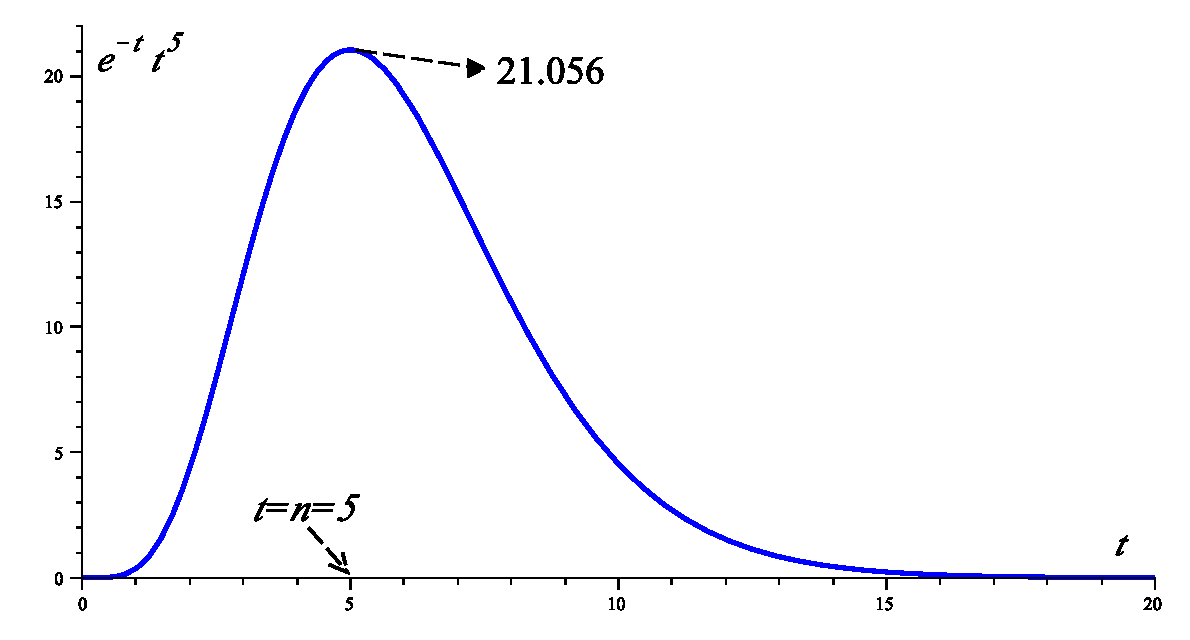
\includegraphics[width=4.5in]{VOLUMEN_2/02_Series/Figuras/gamm}
\caption{ \small La funci�n Gamma para $n=5$}
\label{fGamma}
\end{center}
\end{figure}

Ahora bien, escrito de la forma compacta  se sugiere que el exponente $m$ tendr�a que ser entero y positivo. Pero no es as�. La serie expl�cita  no se restringe a valores enteros y positivos de $m$. Por ello, la forma compacta pero exacta de la expansi�n binomial es 
\begin{eqnarray*}
\left(1 + \frac{x}{a}\right)^m &=&  1 +m\left(\frac{x}{a} \right) + \frac{ m(m-1)}{2}\left(\frac{x}{a} \right)^2 +  \frac{m(m-1)(m-2)}{3!}\left(\frac{x}{a} \right)^3 +\cdots  \\
&=& \sum_{n=0}^{\infty} \frac{\Gamma(1+m)}{\Gamma(1+n)\Gamma(1+m - n)}\left(\frac{x}{a} \right)^n\,. 
\end{eqnarray*}
Donde hemos utilizado la funci�n $\Gamma(x) $ como la generalizaci�n del factorial para valores que no se restringen a enteros positivos. N�tese tambi�n que si el exponente es negativo, $\left(1 + \frac{x}{a}\right)^m$ tiene una singularidad o un polo en $x = -a$.

Cuando $n$ es un entero positivo tendremos 
\[
n!= \Gamma(1 +n)=\int_{0}^{\infty} e^{-t} \, t^n \, \textrm{d}t = \int_{0}^{\infty} e^{-t+n\ln(t)}  \, \textrm{d}t 
\]

Esta integral, como se puede ver en la figura, nos recuerda la forma de una Gaussiana con un m�ximo en 
$t=n$. Al hacer una expansi�n alrededor de este punto
\begin{eqnarray*}
f(t)=-t+n\ln(t) &=& f(n)+(t-n)f'(n)+(t-n)^2f''(n)/2 + \cdots  \\
&=& -n +n\ln(n)+0+(t-n)^2(-n/n^2)/2 + \cdots
\end{eqnarray*}

Si conservamos los t�rminos hasta segundo orden, la integral puede ser aproximadamente igual a:
\[
n! \sim \int_{0}^{\infty} e^{-n +n\ln(n)-(t-n)^2/2n}  \, \textrm{d}t =n^ne^{-n}\int_{0}^{\infty} e^{-(t-n)^2/2n}  \, \textrm{d}t
\]

Para valores de $n$ grandes, y esto es lo que se conoce como la aproximaci�n de Stirling, se tiene:
\[
n! \sim n^ne^{-n} \int_{-\infty}^{\infty}  e^{-(t-n)^2/2n}  \, \textrm{d}t = n^ne^{-n}\sqrt{2\pi n}
\]
Aqu�, el s�mbolo $\sim $ se refiere a un comportamiento asint�tico de la funci�n Gamma.  

En la siguiente tabla se muestran, para algunos valores de $n$, el valor exacto del factorial, el valor por la f�rmula de Stirling y el cociente entre estos dos valores. Se puede apreciar entonces lo buena que resulta tal aproximaci�n.
\begin{table}[h]
  \centering
  \begin{tabular}{@{} |c|c|c|c|@{}} \hline
    $n$ & $n!$  &  $n^ne^{-n}\sqrt{2\pi n}$ &  $n!/(n^ne^{-n}\sqrt{2\pi n})$\\ \hline\hline
    1 & 1 & 0,922 & 0,922 \\ 
    2 & 2 & 1,919 & 0,960 \\ 
    5 & 120 & 118,019 & 0,983 \\ 
  10 & 3628800 & 3598695,619 & 0,992 \\ \hline\hline
  \end{tabular}
  \label{tab:label}
\end{table}

\subsection{Sobre la funci�n Gamma}
Con ya vimos, con la funci�n Gamma es posible generalizar la idea del factorial cuando $n$ es cualquier n�mero real positivo. La funci�n Gamma se define de la siguiente manera
\begin{equation}
\Gamma(k)=\int_{0}^{\infty} x^{k-1} e^{-x}\mathrm{d}x\,,  \quad k> 0 \,.
\label{fungamma}
\end{equation}

Por ejemplo, si $k=1$, tenemos
\[
\Gamma(1)=\int_{0}^{\infty} x^{0} e^{-x}\mathrm{d}x= \lim_{b\rightarrow \infty} \left[ - e^{-x}\ \right]_0^b=1\,.
\]

Podemos integrar (\ref{fungamma}) por partes:
\begin{equation}
\Gamma(k)=   \lim_{b\rightarrow \infty} \left[ \frac{e^{-x}x^k}{k}\ \right]_0^b +
\frac{1}{k} \int_{0}^{\infty} x^{k} e^{-x}\mathrm{d}x\,,  \quad k> 0 \,,
\label{fungamma2}
\end{equation}
se puede demostrar que el primer t�rmino de (\ref{fungamma2}) se hace cero, por lo tanto:
\begin{equation}
\Gamma(k)= \frac{1}{k}  \Gamma(k+1)  \,,  \quad k> 0
\label{fungamma3}
\end{equation}
es decir:
\begin{equation}
\Gamma(k+1)= k \Gamma(k)  \,,  \quad k> 0 \,.
\label{fungamma4}
\end{equation}
Veamos:
\begin{center}
\begin{tabular}
[c]{lll}
$k=1 $ & $\rightarrow$ & $\Gamma(2)=1\Gamma(1)=1=1!$  \\
$k=2 $ & $\rightarrow$ & $\Gamma(3)=2\Gamma(2)=2\cdot1=2!$ \\
$k=3 $ & $\rightarrow$ & $\Gamma(4)=3\Gamma(3)= 3 \cdot  2 \cdot 1=3!$\\
$k=4 $ & $\rightarrow$ & $\Gamma(5)=4\Gamma(4)=4 \cdot  3 \cdot 2 \cdot 1=4!$ \\
\end{tabular}
\end{center}
entonces, si $k=n$ es un entero positivo, se tiene que
\begin{equation}
\Gamma(n+1)= n!
\end{equation}

Ahora bien, podemos hacer lo siguiente. Partimos de (\ref{fungamma3}):
\begin{equation}
\Gamma(k)= \frac{1}{k}  \Gamma(k+1)  \,,  \quad k \neq 0 \,,
\label{fungamma5}
\end{equation}
reemplazamos $k \rightarrow k+1$ en (\ref{fungamma5}) y obtenemos:
\begin{equation}
\Gamma(k+1)= \frac{1}{k+1}  \Gamma(k+2)  \,,  \quad k \neq -1 \,,
\label{fungamma6}
\end{equation}
si sustituimos (\ref{fungamma6}) en (\ref{fungamma5}) resulta:
\begin{equation}
\Gamma(k)= \frac{ \Gamma(k+2)}{k(k+1)}   \,,  \quad k \neq 0, -1 \,,
\label{fungamma7}
\end{equation}
si reemplazamos  $k \rightarrow k+1$ en (\ref{fungamma6}) obtenemos
\begin{equation}
\Gamma(k+2)= \frac{ \Gamma(k+3)}{(k+2)}   \,,  \quad k \neq  -2 \,,
\label{fungamma8}
\end{equation}
al sustituir (\ref{fungamma8})  en (\ref{fungamma7}) resulta lo siguiente
\begin{equation}
\Gamma(k)= \frac{ \Gamma(k+3)}{k(k+1)(k+2)}   \,,  \quad k \neq 0, -1, -2 \,.
\label{fungamma9}
\end{equation}

Estas operaciones se pueden repetir hasta $n$:
\begin{equation}
\Gamma(k)= \frac{ \Gamma(k+n)}{k(k+1)(k+2)\cdots(k+n-1)}   \,,  \quad k \neq 0, -1, -2, \dots , -(n-1) \,.
\label{fungamma10}
\end{equation}

Todo esto sirve para lo siguiente. Si $k=-1/2$, entonces por (\ref{fungamma5}) 
\[
\Gamma\left(-\frac12\right)= -2 \Gamma\left(\frac12\right) \,,
\]
el valor de $\Gamma\left(\frac12\right)$ lo podemos buscar en alguna tabla matem�tica. 


En este caso, lo que se obtiene es $\Gamma\left(\frac12\right)=\sqrt{\pi}$. Esto significa que si  conocemos $\Gamma\left(\frac12\right)$  se puede determinar $\Gamma\left(-\frac12\right)$, por lo tanto
\[
\Gamma\left(-\frac12\right)= -2 \sqrt{\pi} \,.
\]

Algunos ejemplos:
\begin{center}
\begin{tabular}
[c]{rll}
$0!$&=&$\Gamma(0+1)=\Gamma(1)=1$  \\ \\
$\left(-\frac{1}{2}\right)! $&=&$\Gamma(-\frac12+1)=\Gamma\left(\frac12\right)= \sqrt{\pi}$ \\ \\
$\left(-\frac{3}{2}\right)! $&=&$\Gamma(-\frac32+1)=\Gamma\left(-\frac12\right)= -2 \sqrt{\pi}$ \\ \\
$\left(\frac{1}{2}\right)! $&=&$\Gamma(\frac12+1)=\Gamma\left(\frac32\right)=  \frac12 \Gamma\left(\frac12\right)=\frac12 \sqrt{\pi}$ 
\end{tabular}
\end{center}


\subsection{Taylor en varias variables}

S�lo por razones de completitud, y para reforzar los conceptos de que es un desarrollo en series para una funci�n alrededor de un determinado punto, escribiremos el desarrollo en series de Taylor para una funci�n de dos variables $f=f(x,y)$. Esta es
\begin{eqnarray*}
f(x,y)& = & f(a,b) + ( x -a )  \left. f_x \right|_{ ab } + (y-b)\left. f_y \right|_{ ab } \\
    & + & \frac{1}{2!} \left[   \left. ( x -a )^2 f_{xx}  \right|_{ ab } + 2( x -a )( y -a )   \left.  f_{xy} \right|_{ab } +( y -a )^2   \left. f_{yy} \right|_{ ab } \right]\\
 	& + & \frac{1}{3!} \left[ ( x -a )^3  \left. f_{xxx}  \right|_{ ab } + 3( x -a )^2 ( y -a )   \left. f_{xxy} \right|_{ ab } + 3( x -a )( y -a )^2  \left. f_{xyy} \right|_{ ab } +( y -a )^3  \left. f_{yyy}  \right|_{ ab } \right]   \\
	& + & \cdots
\end{eqnarray*}

De una manera  m�s compacta
\[
 f\left( x^j + x_0^j\right)  =  \sum_{n=0}^{\infty} \frac{1}{n!} \left. \left( x^k \partial_{k} \right)^n  f \left( x^m \right)  \right|_{x^m = x^m_0}  \,\, \Rightarrow  \,\,
f\left( { \mathbf{r}} + \mathbf{a}  \right) =  \sum_{n=0}^{\infty}  \frac{1}{n!} \left. \left( \mathbf{r} \cdot {\nabla} \right)^n  f\left( x^m \right)  \right|_{\mathbf{r} = \mathbf{a} }  \,.
\]

D�nde hemos utilizado la siguiente convenci�n
\[
f_{x} = \frac{\partial}{\partial x } = \partial_{x}; \quad f_{y} = \frac{\partial }{ \partial y} = \partial_{y};  \quad f_{xx} = \frac{\partial^2}{\partial x^2 } = \partial_{xx}; \quad f_{xy} = \frac{\partial^2}{\partial x \partial y} = \partial_{xy};  \quad f_{yy} = \frac{\partial^2}{\partial y^2} = \partial_{yy};  \quad \cdots
\]


\subsection{{\color{Fuchsia}Ejemplos}}

\subsection{{\color{red}Practicando con Maxima}}
%\begin{center}
%\begin{boxedminipage}[h]{16.9cm}
La gr�fica mostrada en la Figura 1 pueden obtenerse de la siguiente manera: \\
\textcolor{red}{ $>$ {\tt restart:} } \\
\textcolor{red}{ $>$ {\tt n :=  5:}} \\
\textcolor{red}{ $>$ {\tt f :=  exp(-t)*t$^{\wedge}$n;} } \\
\textcolor{red}{ $>$ {\tt Int(f,t=0..infinity)=int(f,t=0..infinity);} }\\
\textcolor{red}{ $>$ {\tt GAMMA(5+1);} } \\
\textcolor{red}{ $>$ {\tt plot(f,t=0..20); } }\\
\textcolor{red}{ $>$ {\tt `f(5)`=evalf(subs(t=5,f));} }\\
%\end{boxedminipage}
%\end{center}

\subsection{{\color{OliveGreen}Ejercicios}}
\begin{enumerate}
\item Utilice la siguiente definici�n 
\[
\tan^{-1} x = \int_{0}^{x} \frac{1}{1+t^2}\,,
\]
expanda el integrando y luego integre t�rmino por t�rmino para derivar la siguiente
expansi�n conocida como expansi�n de Gregory
\[
\tan^{-1} x = x- \frac{x^3}{3}+\frac{x^5}{5}- \cdots = \sum_{n=0}^{\infty}\frac{(-1)^n}{2n+1} x^{2n+1}\,.
\]
Eval�e  la serie  para $x=\frac{\pi}{4}$.

\item Utilizando la definici�n
\[
\mbox{sen}^{-1} x = \int_{0}^{x} \frac{1}{\sqrt{1+t^2}}\,,
\]
derive las expresiones siguientes
\[
\mbox{sen}^{-1} x =\sum_{n=0}^{\infty} \frac{(2n)!}{4^n (n!)^2} \frac{x^{2n+1}}{2n+1}\,,
\]
$$
\mbox{sen}^{-1} (1-x) = \frac{\pi}{2}-\sqrt{2x}
\left( 1+ \sum_{n=1}^{\infty} \frac{1\mbox{.}  3\mbox{.}   5.  \cdots . (2n-1)}{4^n (2n+1)n!} x^n \right)\,.
$$

\item Encuentre los primeros cinco t�rminos, diferentes de cero, de la serie de Taylor, de la funci�n
\[
f(x)= \frac{1+x}{x^2}\left[\frac{2+2x}{1+2x} - \frac{\ln(1+2x)}{x} \right] \,.
\]
Puedes usar el programa Maxima. 

\end{enumerate}


\section{Series de Fourier}
Otro de los casos de expansi�n en una base completa de funciones lo constituyen la base de Fourier. En este caso la serie de Fourier la constituyen funciones continuas, reales de variable real y definidas en $\left[  0,2\pi\right]  $, $\mathcal{C}_{\left[0,2\pi\right]  }^{\infty}$, en t�rmino de funciones trigonom�tricas. 

Esto es el conjunto de funciones $\left\{  \left| {u}_{1}\right\rangle ,\ \left| {u}_{2}\right\rangle ,\ \left| {u}_{3}\right\rangle ,\cdots,\left| {u}_{n}\right\rangle \cdots\right\}  $ representadas por
\[
\left| {u}_{0}\right\rangle =1,\qquad\left| {u}_{2n}\right\rangle =\cos(nx)\qquad\text{y}\qquad\left| {u}_{2n-1}\right\rangle =\operatorname{sen}(nx),\qquad\text{con }n=1,2,3,\cdots
\]

Es claro que $\left\{  \left| {u}_{1}\right\rangle ,\ \left|{u}_{2}\right\rangle ,\ \left| {u}_{3}\right\rangle \cdots,\left| {u}_{n}\right\rangle ,\cdots\right\}  $  es un conjunto de funciones ortogonales por cuanto
\[
\left\langle{u}_{n}\right.  \left| {u}_{m}\right\rangle
=\delta_{nm} | \left| {u}_{n}\right\rangle|^{2} \Rightarrow \left\{
\begin{array}
[c]{rcl}
0\quad\text{si} & n\neq m & \left\{
\begin{array}
[c]{c}
\int_{0}^{2\pi}\mathrm{d}x\ \operatorname{sen}(nx)\operatorname{sen}(mx)=0 \\ \\
\int_{0}^{2\pi}\mathrm{d}x\ \cos(nx)\operatorname{sen}(mx)=0 \\ \\
\int_{0}^{2\pi}\mathrm{d}x\ \cos(nx)\cos(mx)=0
\end{array}
\right. \\
&  & \\
|  | {u}_{n}\rangle |^{2}\quad\text{si} &
n=m & \left\{
\begin{array}
[c]{lcl}
\int_{0}^{2\pi}\mathrm{d}x\ = 2\pi \\
&  & \\
\int_{0}^{2\pi}\mathrm{d}x\ \cos^{2}(nx)=\pi \\
&  & \\
\int_{0}^{2\pi}\mathrm{d}x\ \operatorname{sen}^{2}(nx)=\pi & 
\end{array}
\right.
\end{array}
\right.
\]

\begin{figure}[t]
\begin{center}
\includegraphics[width=5.6in]{VOLUMEN_2/02_Series/Figuras/FourierSeriesExamples}
\caption{ Expansiones de Varias funciones en sumas parciales de  Series de Fourier. Tomado de Eric W. Weisstein. \textbf{Fourier Series}. \url{http://mathworld.wolfram.com/FourierSeries.html}}
\label{FourierSeriesExamples}
\end{center}
\end{figure}

Por lo tanto, podremos construir una base ortonormal de funciones \newline $\left\{  \left| {e}_{1}\right\rangle ,\ \left| {e}_{2}\right\rangle ,\ \left| {e}_{3}\right\rangle ,\cdots,\left| {e}_{n}\right\rangle ,\cdots\right\}  $ de la forma
\[
\left| {e}_{0}\right\rangle =\frac{1}{\sqrt{2\pi}},\qquad\left|
{e}_{2n}\right\rangle =\frac{1}{\sqrt{\pi}}\cos(nx)\qquad
\text{y}\qquad\left| {e}_{2n-1}\right\rangle =\frac{1}{\sqrt{\pi}
}\operatorname{sen}(nx)
\]

Tal y como se muestra en la figura \ref{FourierSeriesExamples} distintas funciones pueden ser expandidas con sumas parciales de Fourier.  A diferencia de las series de potencias, que imponen que las funciones a ser expandidas deben ser continuas y continuamente diferenciables en el intervalo, la series de Fourier pueden representar funciones continuas a trozos, siempre y cuando cumplan con algunas condiciones.

Por lo tanto cualquier funci�n definida en el intervalo $\left[ 0,2\pi\right]  $ puede expresarse en t�rminos de esta base como
\[
\left| {f}\right\rangle = \sum_{i=0}^{\infty}  c_{i}\ \left|{e}_{i} \right\rangle \quad \Rightarrow 
c_{i} = \left\langle{e}_{i} \right.  \left| {f}\right\rangle =
\left\{
\begin{array}[c]{lcl}
\frac{1}{\sqrt{2\pi} } \int_{0}^{2\pi} \mathrm{d}x  \ f(x)  = c_{0} \equiv a_{0} & \text{si} & i=0 \\
&  & \\
\frac{1}{\sqrt{\pi} } \int_{0}^{2\pi}\mathrm{d}x\ f( x)  \ \cos(nx) = c_{2n} \equiv a_{m} & \text{si} & i=2n\\
&  & \\
\frac{1}{\sqrt{\pi} } \int_{0}^{2\pi}\mathrm{d}x\ f( x )  \ \operatorname{sen}(nx) = c_{2n-1} \equiv b_{m} & \text{si} & i=2n-1
\end{array}
\right.
\]
donde los $c_{i}$ son los coeficientes de Fourier, con lo cual podemos escribir
\[
F(x) = \frac{a_{0}}{2} +  \sum_{n=1}^{\infty} \left[ a_{n} \cos(nx) + b_{n} \mathrm{sen}(nx) \right] \,,
\]
el t�rmino $a_0$ es colocado fuera de la sumatoria, y multiplicado por $1/2$, solo por conveniencia.

De manera equivalente, si el per�odo es $T$ y para un $t_{0}$ gen�rico
\[
F(t) = \frac{a_{0}}{2} +  \sum_{n=1}^{\infty} \left[ a_{n} \cos \left( \frac{2 \pi nt}{T} \right) + b_{n} \mathrm{sen}\left( \frac{2 \pi nt}{T} \right) \right] \quad \text{con }
\left\{
\begin{array}{cl}
   a_{0} =  & \frac{2}{T} \int_{t_{0}}^{t_{0} + T} \mathrm{d}t  \ f(t) \\
  & \\
   a_{n} =  &  \frac{2}{T} \int_{t_{0}}^{t_{0} + T} \mathrm{d}x\ f(t) \cos \left( \frac{2 \pi nt}{T} \right)   \\
    & \\
   b_{n} =  &  \frac{2}{T} \int_{t_{0}}^{t_{0} + T}\mathrm{d}t\ f(t) \ \mathrm{sen} \left( \frac{2 \pi nt}{T} \right)  
\end{array}
\right. 
\]

La figura \ref{FourierSeriesExamples} muestra la aproximaci�n de las distintas sumas parciales para distintas funciones, a medida que aumentamos el n�mero de t�rminos la aproximaci�n mejora.

Podemos expresar la expansi�n de una serie de Fourier de manera m�s compacta, �sta expresi�n se conoce en algunos �mbitos como la expresi�n integral para la series de Fourier
\begin{eqnarray}
F(x)	& = & \frac{1}{\sqrt{2 \pi} } \int_{0}^{2\pi} \mathrm{d}t  \ f(t)  \nonumber \\
 	& + &   \sum_{n=1}^{\infty}  \left\{ \left[ \int_{0}^{2\pi}\mathrm{d}t \ f(t)  \cos(nt) \right]\cos(nx) + \left[ \int_{0}^{2\pi}\mathrm{d}t \ f(t) \operatorname{sen}(nt) \right] \mathrm{sen}(nx) \right\} 											\nonumber \\
	 	&  &  	\nonumber \\
  	& = &  \frac{1}{\sqrt{2 \pi} } \int_{0}^{2\pi} \mathrm{d}t  \ f(t)  +  \sum_{n=1}^{\infty} \int_{0}^{2\pi}\mathrm{d}t \ f( t)  \cos(n[t-x]) \,.
 \nonumber
\end{eqnarray}

Tambi�n es muy com�n expresar una serie de Fourier en t�rmino de una base compleja. Vale decir  $ \big\{ \cdots | \mathbf{ \tilde{\phi} }_{k}  \rangle \cdots \big\} \leftrightarrow \{ \cdots e^{-ikx} \cdots \}   $ con $k=0,\pm1,\pm2,\cdots$. Con lo cual 
\[
|{f} \rangle = \sum_{k=-\infty }^{\infty}  \tilde{C}_{k} |{\tilde{\phi}}_{k} \rangle \equiv \sum_{k=-\infty }^{\infty}  \tilde{C}_{k} e^{-ikx} \qquad \text{con} \quad
\tilde{C}_{k}  = \frac{ \langle{ \tilde{\phi}}_{k} | {f}  \rangle  }{ \langle{\tilde{\phi}}_{k} |{\tilde{\phi}}_{k}  \rangle} = \frac{1 }{2 \pi} \int_{-\pi}^{\pi} \mathrm{d}x \ e^{-ikx} f(x)\,.
\]

Podremos reescribir (una vez m�s) la expresi�n de una suma parcial de la serie de Fourier, dado que 
\[
a_{n}\cos(nx) + b_{n} \operatorname{sen}(nx) = \frac{1}{\pi} \int_{-\pi}^{\pi} \mathrm{d}t  \ f(t) \cos(n[t-x]) \,,
\]
tendremos que
\begin{eqnarray}
F_{n}(x) & = &  \frac{a_{0}}{2} +  \sum_{k=1}^{n} \left[ a_{k} \cos(kx) + b_{k} \mathrm{sen}(kx) \right] =  \frac{a_{0}}{2} +  \sum_{k=1}^{n} \left[ \frac{1}{\pi} \int_{-\pi}^{\pi} \mathrm{d}t  \ f(t) \cos(n(t-x)) \right]  \nonumber \\
 & = & \Re \left[  \int_{-\pi}^{\pi} \mathrm{d}t  \ f(t) \Big\{ \frac{1}{2} + \sum_{k=1}^{n} \left( 
 e^{-i(t-x)k}
 \right) \Big\} \right]  \,.
 \nonumber
\end{eqnarray}
y al sumar la progresi�n geom�trica que representa una serie de exponenciales llegamos a
\[
F_{n}(x)  = \frac{1}{2 \pi} \int_{-\pi}^{\pi} \mathrm{d}t \ f(t)
 \left[ \dfrac{ \operatorname{sen}\left( \left( n +\frac{1}{2} \right)(t -x)  \right)}{ \operatorname{sen}\left( \frac{1}{2}(t -x)  \right)}  \right] \equiv  \frac{1}{2 \pi} \int_{-\pi}^{\pi} \mathrm{d}t \ f(t) \ \mathcal{K}(x,n,t)\,,
\]
la cual siempre es convergente y el t�rmino 
\[
\mathcal{K}(x,n,t) = \left[ \dfrac{ \operatorname{sen}\left( \left( n +\frac{1}{2} \right)(t -x)  \right)}{ \operatorname{sen}\left( \frac{1}{2}(t -x)  \right)}  \right] \,,
\] 
se conoce como el n�cleo de la transformaci�n de $F$, el \textit{Kernel} de Dirichlet.

La pregunta b�sica que sigue es, en todos estos casos: �c�mo se relaciona la expansi�n de Fourier $\left|  {f}\right\rangle \Leftrightarrow F(x)$ con la funci�n $f(t)$ que genera los coeficientes de la expansi�n? N�tese que es una forma de mirar una relaci�n entre $F(x) \leftrightarrow f(t)$.  Pasamos de $f(t)$ a $F(x)$ mediante una ``transformaci�n'' 
\[
F_{n}(x)  = \frac{1}{2 \pi} \int_{-\pi}^{\pi} \mathrm{d}t \ f(t) \ \mathcal{K}(x,n,t)\,.
\]

Este tipo de relaciones se denomina transformaci�n integral y en particular �sta es una de las expresiones de las llamadas \textit{Transformadas de Fourier}.

\begin{figure}[h]
\begin{center}
\includegraphics[width=6.9in]{VOLUMEN_2/02_Series/Figuras/Cuadratura_Gauss}
\end{center}
\end{figure}

\subsection{Condiciones de Dirichlet}

Las condiciones que una determinada funci�n $f(x)$ debe cumplir para poder ser representada como una serie de Fourier, se conocen con el nombre de condiciones de Dirichlet\footnote{\textbf{Johann Peter Gustav Lejeune Dirichlet} 1805 - 1859. Matem�tico Alem�n con importantes contribuciones en Teor�as de n�meros Algebraica, Series y aproximaciones de funciones y ecuaciones diferenciales parciales.} las cuales pueden ser esquematizadas en los siguientes puntos:
\begin{itemize}
\item la funci�n $f(x)$ debe ser peri�dica
\item la funci�n $f(x)$ debe se univaluada y continua a trozos (continua menos, en un n�mero finito de puntos) con  un n�mero finito de m�ximos y m�nimos
\item la integral $\int_{-T/2}^{T/2} \mathrm{d}x |f(x)|$ debe ser convergente. Donde $\left[ -T/2, T/2 \right]$ quiere indicar el intervalo de definici�n de una funci�n con per�odo $T$.
\end{itemize}

Podemos formalizar un poco m�s las condiciones de Dirichlet en el llamado teorema de Fourier.
\begin{mdframed}[linecolor=OliveGreen,linewidth=0.3mm]
\textbf{Teorema de Fourier}: Sea $f(x)$ una funci�n en el intervalo $-\pi \leq x \leq \pi$ y definida para el resto de la recta real tal que cumpla con $f(x +2\pi) = f(x)$. Es decir $f(x)$ es $2\pi-$peri�dica. Supongamos adem�s que existe la integral
\[
\int_{-\pi}^{\pi} \mathrm{d}x \  f(x)\,, \quad \text{y que} \quad {C}_{k}  = \frac{1 }{2 \pi} \int_{-\pi}^{\pi} \mathrm{d}x \ e^{-ikx} f(x) \quad  \text{con } k=0,\pm1,\pm2,\cdots.
\]  
y si $|f(x)|$ est� acotada para un intervalo $[a,b]$ con $-\pi < a \leq x \leq b < \pi$, entonces
\[
F(x) = \sum_{k=-\infty }^{\infty}  {C}_{k} e^{-ikx} \quad \text{es convergente al valor  }
F(x) = \frac{1}{2} \left( \lim_{\epsilon \rightarrow 0_{+}} f(x + \epsilon ) +  \lim_{\epsilon \rightarrow 0_{-}} f(x - \epsilon ) \right)
\]
y si $f(x)$ es continua en $x=x_{0}$ entonces $ F(x_{0}) \rightarrow f(x_{0})$.
\end{mdframed}

En este punto se pueden puntualizar varias cosas:
\begin{enumerate}
\item El valor $F(x) = \frac{1}{2} \left( \lim_{\epsilon \rightarrow 0_{+}} f(x + \epsilon ) +  \lim_{\epsilon \rightarrow 0_{+}} f(x - \epsilon ) \right)$ al cual converge la expansi�n de Fourier, cobra particular importancia cuando el punto $x =x_{0}$ es una discontinuidad. Tal y como veremos m�s adelante (secci�n \ref{FourierDiscontinuidad}) y expresa este teorema, las series de Fourier son particularmente apropiadas para expandir funciones discontinuas (en un n�mero finito de puntos en el intervalo), sin embargo, por ser una base de funciones continuas no puede reproducir la discontinuidad como tal. La expansi�n de Fourier alrededor de un punto de discontinuidad $x \rightarrow x_{\pm 0}$ tender� al valor $F(x) \rightarrow F(x_{\pm 0}) \equiv F_{m}$ donde $F_{m} = \frac{F(x_{+ 0}) + F(x_{- 0}) }{2}$. Es decir, tender� al valor medio de los valores de la discontinuidad por la izquierda $F(x_{- 0}) $ y por la derecha $F(x_{+ 0}) $.  
 \item Si los coeficientes de Fourier tienen variaciones acotadas en el intervalo y $|{C}_{k}  | \rightarrow 0$  con $k \rightarrow \infty $. Entonces 
\[
 \sum_{k=-\infty }^{\infty} | {C}_{k} |^{2} =  \frac{1 }{2 \pi} \int_{-\pi}^{\pi} \mathrm{d}x \ | f(x) |^{2}
 \qquad \Leftrightarrow \qquad \frac{1}{2} a_{0}^{2} +  \sum_{n=1 }^{\infty} | a_{n}^{2} + b_{n}^{2} |=  \frac{1 }{\pi} \int_{-\pi}^{\pi} \mathrm{d}x \ | f(x) |^{2} \,,
\]
que no es otra cosa que la expresi�n de la completitud de esta base de funciones. 
\end{enumerate}

Para ilustrar esta relaci�n entre la funci�n $f(x)$ y su expansi�n en serie de Fourier $F(x)$ analicemos el siguiente ejemplo 

La siguiente funci�n, muy conocida en el �mbito de los circuitos el�ctrico, se denomina la funci�n onda cuadrada
\[
f(t)=
\left\{
\begin{array}{rl}
    -1  & \text{si } -\frac{1}{2}T \leq t <  0   \\
      &    \\
    +1  & \text{si } 0 \leq t \leq \frac{1}{2}T \,,
\end{array}
\right.
\]

En este caso se puede integrar entre $[0,T/2]$ y luego multiplicar todo por $2$.
\begin{eqnarray*}
a_{0} &=& \frac{2}{T} \int_{0}^{\frac{T}{2}} \mathrm{d}t = 1 \,, \quad 
a_{n} = \frac{2}{T} \int_{0}^{\frac{T}{2}} \cos\left( \frac{2 \pi n t}{T} \right) \mathrm{d}t = 
\frac{\mathrm{sen}\left(n \pi  \right)}{n\pi} =0 \,,\\
b_{n} &=&   \frac{2}{T} \int_{0}^{\frac{T}{2}}\mathrm{sen}\left(\frac{2 \pi n t}{T} \right)\mathrm{d}t 
= \frac{1- \cos\left(n \pi  \right)}{n\pi} = \frac{1- (-1)^{n}}{n \pi}\,,
\end{eqnarray*}

Entonces solo sobreviven los $b_{2n+1}$ ya que coeficientes pares se anulan:  $b_{2n}=0$.
\[
f(t)= {a_0} + 2\sum_{n=1}^{\infty} b_n \mathrm{sen}\left(\frac{2 \pi n t}{T} \right)= 
1+\frac{4}{\pi} \left(\mathrm{sen}( \omega t) + \frac{\mathrm{sen}(3 \omega t)}{3} + 
\frac{\mathrm{sen} (5 \omega t)}{5} +  \frac{\mathrm{sen}(7 \omega t)}{7} + \cdots \right)
\]
donde hemos denotado $\omega = 2 \pi/ T $. 

Al definir la funci�n $\omega$ podemos interpretar los coeficientes de Fourier $a_{n},b_{n}$ como las contribuciones de cada uno de los arm�nicos $a_{n},b_{n} \rightarrow \omega_{n} = \frac{2 n \pi}{T} $. A partir de estas contribuciones se construye el espectro de potencia, el cual est� relacionado con la energ�a que aporta cada uno de estos arm�nicos. Por ello construimos un cantidad $E_{n} = \sqrt{a_{n}^{2} + b_{n}^{2}}$ y graficamos $E_{n}$ vs $n$ tal y como se puede comprobar en la figura \ref{FigSeriesFourier}, cuadrantes IV y VII. Se encuentra que se puede asociar un espectro de potencia a cada se�al y con lo cual realizar una especie de identificaci�n.

En este punto podemos hacernos algunas preguntas: 
\begin{itemize}
 \item �qu� hubiera pasado si en vez de considerar el intervalo $\left( -\frac{T}{2},\frac{T}{2} \right)$ hubi�ramos considerado $\left( 0, T \right)$?
 \item �tendr�amos el mismo desarrollo en serie de Fourier?
 \item �el mismo espectro?
\end{itemize}
Justifique sus respuestas.


\subsection{Consideraciones de simetr�a en series de Fourier}
Es de hacer notar que estas propiedades de simetr�a respecto al per�odo de la funci�n ($f(x) = f(-x)$ simetr�a y $f(x) = -f(-x)$ antisimetr�a) para un per�odo $-\frac{T}{2} \leq x \leq \frac{T}{2}$ pueden y deben ser explotadas para simplificar los c�lculos. Esto se puede resumir en 
\[
f(x) = f(-x) \,\, \Rightarrow \,\,
\left\{ 
\begin{array}{l}
  a_{n} \neq 0      \\
  b_{n} = 0        
\end{array}
\right. \quad \text{y alternativamente} \quad
f(x) = -f(-x) \,\, \Rightarrow \,\, 
\left\{ 
\begin{array}{ l}
  a_{n} = 0      \\
  b_{n}  \neq 0        
\end{array}
\right.
\]

Pero m�s interesante a�n es cuando estas propiedades de simetr�a se presentan en un cuarto  del per�odo. Vale decir, que $f(x)$ ser� par o impar respecto a $T/4$ i.e. $f\left( \frac{T}{4} +x \right) = \pm f\left( \frac{T}{4} -x \right) \Rightarrow f(-s) = \pm f(s)$ donde $s = \frac{T}{4} -x$. Entonces
\[
 b_{n} =   \frac{2}{T} \int_{x_{0}}^{x_{0} + T} \mathrm{d}s \ f( s) \ \mathrm{sen} \left( \frac{2 \pi ns}{T}  + \frac{\pi n}{2} \right) \,.
\]

Donde los l�mites de integraci�n no se han visto alterados porque la funci�n es peri�dica. Es inmediato comprobar que 
\[
\mathrm{sen} \left( \frac{2 \pi ns}{T}  + \frac{\pi n}{2} \right)  =
\mathrm{sen} \left( \frac{2 \pi ns}{T} \right)  \cos \left( \frac{\pi n}{2} \right) + 
 \cos \left( \frac{2 \pi ns}{T} \right)   \mathrm{sen} \left( \frac{\pi n}{2} \right) \,,
\]
es decir 
\[
b_{n} =   \frac{2}{T} 
\left[
\cos \left( \frac{\pi n}{2} \right) \int_{x_{0}}^{x_{0} + T} \mathrm{d}s \ f( s) \mathrm{sen} \left( \frac{2 \pi ns}{T} \right)   + 
\mathrm{sen} \left( \frac{\pi n}{2} \right) \int_{x_{0}}^{x_{0} + T} \mathrm{d}s \ f( s) \ \cos \left( \frac{2 \pi ns}{T} \right)   
\right] \,,
\]
por lo que si $n =2k \Rightarrow \mathrm{sen} \left( \frac{\pi n}{2} \right) = \mathrm{sen}( \pi k ) = 0 $  y si $n =2k-1 \Rightarrow \cos \left( \frac{ 2k-1}{2} \pi\right) = 0 $. 

La misma consideraci�n se puede hacer para los coeficientes $a_{n}$ (queda como ejercicio para el lector) y se puede concluir que 
\begin{itemize}
  \item Si $f(x)$ par en $T/4$ entonces $a_{2n -1} = b_{2n} = 0$.
  \item Si $f(x)$ impar en $T/4$ entonces $a_{2n} = b_{2n-1} = 0$.
\end{itemize}


\subsection{El Fen�meno de Gibbs}
\label{FourierDiscontinuidad}

Tal y como hemos mencionado, a diferencia de las series de potencias, las series de Fourier manejan razonablemente bien las discontinuidades, pero por ser una base de funciones continuas, no puede reproducirlas. Tal y como comentamos en el Teorema de Fourier  y muestra la figura \ref{EscalonFourier} el valor de las sumas parciales de Fourier en un punto de discontinuidad $x = x_{\pm 0}$ ser� el promedio de los valores $F(x_{- 0}) $ (por la izquierda) y $F(x_{+ 0}) $ (por la derecha)  en la discontinuidad.  Esto es la expansi�n de Fourier alrededor de un punto de discontinuidad $x \rightarrow x_{\pm 0}$ tender� al valor $F(x) \rightarrow F(x_{\pm 0}) \equiv F_{m}$ donde $F_{m} = \frac{F(x_{+ 0}) + F(x_{- 0}) }{2}$. 


Podemos ver  en la figura \ref{EscalonFourier} que, tanto por la izquierda como por la derecha de la discontinuidad de la funci�n escal�n, las sumas parciales de Fourier oscilan y no convergen a los valores $x_{\pm 0}$. El comportamiento oscilante de las sumas parciales de Fourier alrdedor de las discontinuidades, que no desaparecen ni en el l�mite se   denominan \textit{fen�meno de Gibbs} en honor a su descubridor Josiah Willard Gibbs.\footnote{\textbf{Josiah Willard Gibbs} 1839 - 1903. Algunos lo consideran el primer F�sico Norteamericano, de hecho fue el primero en recibir un t�tulo de doctorado por una universidad norteamericana (Yale University). Hizo importantes aportes en electromagnetismo  y sobre todo en termodin�mica y f�sica estad�stica, sentando las bases matem�ticas para estas disciplinas. En matem�ticas es conocido su estudio de las oscilaciones de las expansiones de las series de Fourier en los puntos de discontinuidad.}

Para entender qu� pasa en la discontinuidad consideremos una variaci�n de la onda cuadrada considerada anteriormente (\ref{FourierEjemplos}). Entonces sus sumas parciales ser�n
\[
f(t)=
\left\{
\begin{array}{rl}
    1  & \text{si } 0 \leq t <  \pi   \\
      &    \\
    0  & \text{si } \pi \leq t < 2 \pi      
\end{array}
\right. \,\, \Rightarrow \,\, F_{2n}^{c}(x) = \frac{1}{2} + \frac{2}{\pi} \sum_{k=1}^{n} \frac{1}{2k - 1}
\mathrm{sen}\left((2k - 1)x\right) \,, 
\]
porque los coeficientes pares ($a_{n}$) se anulan. 

Para estudiar el fen�meno de Gibbs reescribimos la suma parcial anterior de una manera ingeniosa 
\[
F_{2n}^{c}(t) =   \frac{1}{2} +  \frac{2}{\pi} \sum_{k=1}^{n} \left( \int_{0}^{t} \mathrm{d}s \ \cos(2k -1)s \right) =  
 \frac{1}{2} +  \frac{2}{\pi} \int_{0}^{t} \mathrm{d}s \left( \sum_{k=1}^{n} \cos(2k -1)s  \right) = 
  \frac{1}{2} +  \frac{1}{\pi} \int_{0}^{t} \mathrm{d}s \left( \frac{ \mathrm{sen}(2ns)}{ \mathrm{sen}( s)} \right)
\]
donde, utilizando la f�rmula de Moivre y convirtiendo esa serie de cosenos en una de exponenciales la cual, a su vez es una progresi�n geom�trica (y le queda la comprobaci�n al lector), hemos sustituido
\[
\sum_{k=1}^{n} \cos(2k -1)s = \frac{ \mathrm{sen}(2ns)}{ \mathrm{sen}( s)}\,.
\]

Es inmediato convencerse que las sumas parciales $F_{2n}^{c}(x)$ siempre tendr�n m�ximos y m�nimos 
\[
\dfrac{ \mathrm{d} F_{2n}^{c}(x)}{ \mathrm{d}x} =  \frac{ \mathrm{sen}(2nx)}{ \mathrm{sen}( x)} = 0 
\\,\, \Rightarrow \,\, \text{para  }
x = \frac{m \pi}{2n } \quad \text{con } m=1,2,3,\cdots 
\]

Las Series de Fourier tienden a sobre-estimar el valor de los puntos de discontinuidad en $\pm 18 \%$ esto es un valor de $\approx 1.1789797$. La inclusi�n de m�s t�rminos en las sumas parciales no mejoran la situaci�n. El fen�meno de Gibbs no se restringe a Series de Fourier sino que tambi�n se presenta en las dem�s series de funciones (ver detalles en la referencia: {\tt Arfken-Weber-2000}) .

El fen�meno de Gibbs fue observado �experimentalmente! por primera vez por Albert Michelson.\footnote{\textbf{Albert Abraham Michelson} Strelno, Prussia, 1852 - Pasadena EEUU. 1931. Premio Nobel en F�sica (1907) uno de los f�sicos experimentales m�s habilidosos de todos los tiempos. La precisi�n y lo ingenioso de los instrumentos creados por �l son famosos.  Con importantes contribuciones en medidas de fen�menos en �ptica. Una de sus contribuciones m�s conocidas son los experimentos para mostrar la inexistencia del Ether como medio de transmisi�n para el fen�meno electromagn�tico. M�s detalles \url{http://nobelprize.org/physics/laureates/1907/michelson-bio.html}}.  Para finales de 1800 Michelson hab�a creado un dispositivo mec�nico para medir las componentes de Fourier de se�ales el�ctricas. Al incorporarle una onda cuadrada observ� que una oscilaci�n inesperada en los puntos de discontinuidad. Crey� que esa oscilaci�n se deb�a a defectos del dispositivo. Luego de probar m�ltiples tipos de se�ales peri�dicas y observar un comportamiento similar, decidi� coment�rselo a su amigo Willard Gibbs, de la Universidad Yale. Al poco tiempo Gibbs volvi� con una explicaci�n que dej� intacta la fama de Michelson como instrumentista. El fen�meno es una consecuencia de la teor�a de series de Fourier y no del equipo dise�ado por Michelson\footnote{M�s detalles \url{http://en.wikipedia.org/wiki/Gibbs_phenomenon}}. 

\begin{figure}[t]
\begin{center}
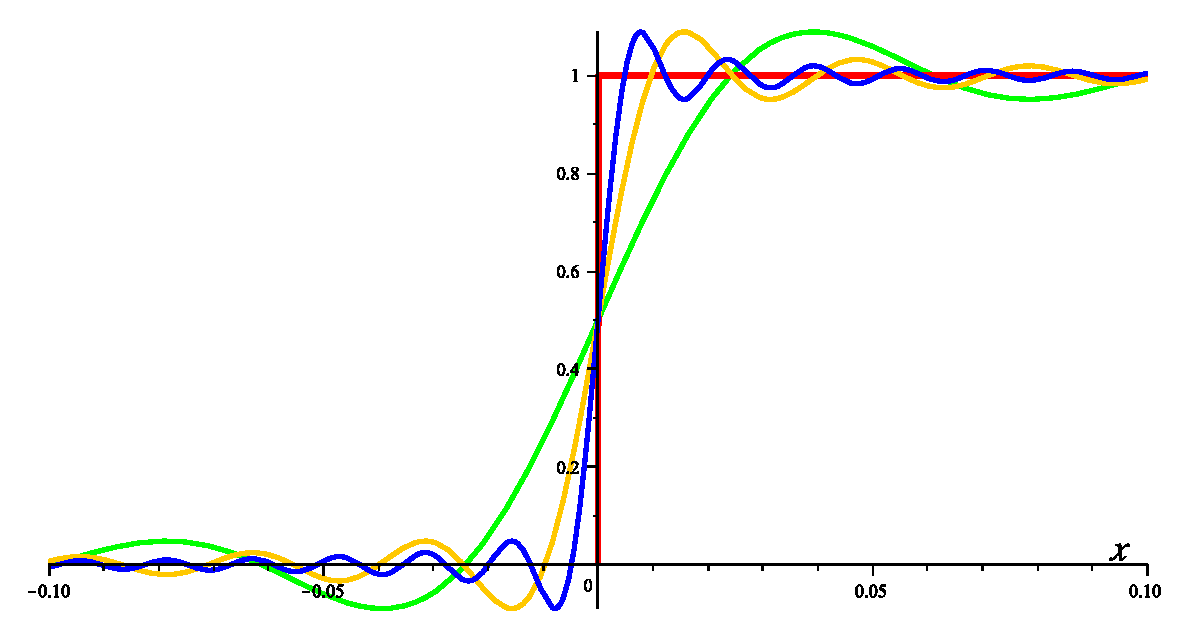
\includegraphics[width=4.0in]{VOLUMEN_2/02_Series/Figuras/escalonfourier.eps}
\caption{ Aproximaciones por series de Fourier para la funci�n escal�n, linea roja.  Las curvas corresponden a sumas parciales de Fourier: $F_{40}(x), F_{100}(x), F_{200}(x), $ }
\label{EscalonFourier}
\end{center}
\end{figure}


\subsection{Correcci�n al fen�meno de Gibbs: Factor $\sigma$ de Lanczos}
Una de las estrategia para corregir las oscilaciones del fen�meno de Gibbs se le debe a Lanczos\footnote{\textbf{Cornelius Lanczos} 1893 - 1974 Hungr�a. Matem�tico h�ngaro con contribuciones importante en Relatividad y F�sica Te�rica. En matem�ticas es conocido inventar la transformada r�pida de Fourier. M�s detalles en \url{http://www-history.mcs.st-and.ac.uk/Biographies/Lanczos.html}}. Considerando el mismo caso de la funci�n onda cuadrada, se puede intentar sustituir la funci�n oscilante $F_{n}^{c}(x)$ por su promedio $\bar{F}_{n}^{c}(x)$ alrededor del punto $x$. Vale decir
\[
F_{2n}^{c}(x) \rightarrow \bar{F}_{2n}^{c}(x) = \frac{n}{\pi}  \int_{x - \frac{\pi}{2n} }^{x + \frac{\pi}{2n} } \mathrm{d}s \ F_{2n}^{c}(s) =  \frac{n}{\pi}  \int_{x - \frac{\pi}{2n} }^{x + \frac{\pi}{2n} } \mathrm{d}s \left[ \frac{1}{2} + \frac{2}{\pi} \sum_{k=1}^{n} \frac{1}{2k - 1} \mathrm{sen}((2k - 1)s) \right]\,,
\]
desarmando tendremos que 
\begin{eqnarray}
\bar{F}_{2n}^{c}(x) & = &   \frac{n}{\pi}  \int_{x - \frac{\pi}{2n} }^{x + \frac{\pi}{2n} } \mathrm{d}s \left[ \frac{1}{2} + \frac{2}{\pi} \sum_{k=1}^{n} \dfrac{1}{2k - 1} \mathrm{sen}((2k - 1)s) \right] 
\nonumber \\
 & = &  \frac{n}{\pi} \left[ \frac{\pi}{2n} + \frac{2}{\pi} \sum_{k=1}^{n}  \left. \dfrac{1}{(2k - 1)^{2}} \cos((2k-1)s) \right|_{x - \frac{\pi}{2n} }^{x + \frac{\pi}{2n} }  \right] \nonumber \\
\bar{F}_{2n}^{c}(x) & = &  \frac{1}{2} + \frac{2}{\pi}  \sum_{k=1}^{n}  \dfrac{1}{2k - 1}
\underbrace{ \left[ \dfrac{ \mathrm{sen}\left( \frac{\pi}{2n} (2k - 1) \right) }{\frac{\pi}{2n}(2k - 1)}\right] }_{\sigma} \mathrm{sen}((2k - 1)x) \,.
\nonumber
\end{eqnarray}

Con lo cual hemos identificado el factor $\sigma$ de Lanczos. Siguiendo este mismo proceso se puede generalizar para cualquier funci�n de tal modo que una serie de Fourier gen�rica podr� ser corregida con un factor $\sigma$ para lograr
\[
\bar{F}_{n}(x) =  \frac{a_{0}}{2} +  \sum_{k=1}^{n-1} 
\left[ \dfrac{ \mathrm{sen}\left( \frac{k\pi}{n} \right) }{\left( \frac{k\pi}{n} \right) } \right]
 \left( a_{k} \cos (kx) + b_{k} \mathrm{sen} (kx) \right) \equiv
  \frac{a_{0}}{2} +  \sum_{k=1}^{n-1} \sigma_{k} \left( a_{k} \cos (kx) + b_{k} \mathrm{sen} (kx) \right)\,.
\]


\subsection{{\color{Fuchsia}Ejemplos}}

\begin{enumerate}
\item {\bf Variedades de dientes de sierra}

Otra funci�n muy com�n es la denominada dientes de sierra
\[
f(t)= a t  \quad \text{si } 0 \leq t \leq  T  \,, \quad \text{con } a \text{ constante }
\] 
los coeficientes son los siguientes:
\begin{eqnarray*}
a_{0} &=& \frac{2}{T} \int_{0}^{T}a t \mathrm{d}t  = a T \,,\\
a_{n} &=& \frac{2}{T} \int_{0}^{T}a t \cos \left( \frac{2 \pi nt}{T}\right) \mathrm{d}t  = 
{\frac {a\,T}{{\pi }^{2}{n}^{2}}} \left[ n \pi \mathrm{sen} \left( 2 n\,\pi \right) -
\mathrm{sen}^2 \left(n \pi  \right)\right]=0\,,\\
b_{n} &=& \frac{2}{T} \int_{0}^{T}a t\,\mathrm{sen}\left(\frac{2\pi nt}{T}\right)\mathrm{d}t  = 
-\frac {a T}{n\,\pi} \,.
\end{eqnarray*}

Tenemos entonces que
\[
f(t)= at=\frac{a_0}{2} + \sum_{n=1}^{\infty} b_n \mathrm{sen}\left(\frac{2 \pi n t}{T} \right)= 
\frac{aT}{2} - \frac{aT}{\pi} \sum_{n=1}^{\infty} \frac{\mathrm{sen}\left(\omega n t \right)}{n} \,
 \,,\quad \text{para } 0 \leq t \leq  T \,.
\]

\begin{figure}[t]
\begin{center}
\includegraphics[width=6.0in]{VOLUMEN_2/02_Series/Figuras/VariosFourier}
\caption{Un par de funciones, definidas con un per�odo $T$, a ser expresadas en como expansiones en Series de Fourier. En los cuadrantes I y II, encontramos una onda cuadrada. La primera (cuadrante I) definida en un intervalo $\left( -\frac{T}{2}, \frac{T}{2} \right)$  y en el cuadrante II la misma funci�n definida en un intervalo $( 0, T )$. El cuadrante III ilustra las aproximaciones de la serie de Fourier para $n=3,7,20$, mientras que el espectro de potencia se presenta en el cuadrante IV. La onda ``diente de sierra'', definida en un intervalo $\left( 0, T \right)$, se presenta en el cuadrante V. Sus aproximaciones en series de Fourier para $n=3,7,10$ se pueden observar en el cuadrante VI, mientras que el espectro de potencia en el cuadrante VII. }
\label{FigSeriesFourier}
\end{center}
\end{figure}


En el caso particular de hacer $a =3$ y $T = 2 \rightarrow \omega_{n} = n \pi $, entonces:
\[
f(t)= 3t= 3 - \frac{6}{\pi} \sum_{n=1}^{\infty} \frac{\mathrm{sen}\left(n \pi t \right)}{n} = 
3- {\frac {6\mathrm{sen} \left( \pi \,t \right) }{\pi }} - {\frac {3 \mathrm{sen} \left( 2\,\pi \,t \right) }{\pi }} - {\frac {2\mathrm{sen} \left( 3\,\pi \,t \right) }{\pi }} - {\frac {3\mathrm{sen} \left( 4\,\pi \,t \right) }{2\pi }}
- {\frac {6 \mathrm{sen} \left( 5\,\pi \,t \right) }{5 \pi }} + \cdots
\]

La figura \ref{FigSeriesFourier} (cuadrantes V y VI) muestra la construcci�n de esta funci�n y su representaci�n en Series de Fourier. 

A partir de esta funci�n podemos hacer unas variaciones. Por ejemplo consid�rese la funci�n 
\[
f(t)= a t  \quad \text{si } \frac{-T}{2} \leq t \leq  \frac{T}{2} \,, \quad \text{con } a \text{ constante }
\quad \Rightarrow 
\left\{
\begin{array}{cll}
   a_{0} =  & \frac{2}{T}\int_{-T/2}^{T/2}a t \mathrm{d}t  & = 0 \\   \\
   a_{n} =  & \frac{2}{T}\int_{-T/2}^{T/2}a t \cos\left(\frac{2\pi nt}{T}\right) \mathrm{d}t & = 0\\  \\
   b_{n} =  & \frac{2}{T}\int_{-T/2}^{T/2}a t\,\mathrm{sen}\left(\frac{2\pi nt}{T}\right)\mathrm{d}t & = 
   -\frac {a T(-1)^{n}}{n\,\pi}\,.
\end{array}
\right. 
\] 

Claramente es una funci�n impar $f(-x) = -f(x)$ y as� lo refleja su expansi�n en series de Fourier. Si hacemos $ a =3$ y $T = 2 \rightarrow \omega_{n} = n \pi $ tendremos que la expresi�n para de la serie es 
\[
f(t)= 3 t = {\frac {6\mathrm{sen} \left( \pi \,t \right) }{\pi }} -{\frac {3 \mathrm{sen} \left( 2\,\pi \,t \right) }{\pi }} + {\frac {2 \mathrm{sen} \left( 3\,\pi \,t \right) }{\pi }} - {\frac{3 \mathrm{sen} \left( 4\,\pi \,t \right) }{2\pi }} + {\frac {6\mathrm{sen} \left( 5\,\pi \,t \right) }{5\pi }} + \cdots
 \quad \text{con } \frac{-T}{2} \leq t \leq  \frac{T}{2} \,,
\] 
la cual, si bien es parecida no es igual a la anterior, debido que estamos expandiendo otra funci�n.

Otra variaci�n posible de la funci�n ``diente de sierra'' puede ser la versi�n completamente par  del ``diente'', $f(-x) = f(x)$. Esta es
\[
f(t)= 
\left\{
\begin{array}{l}
   -a t  \quad \text{si } \frac{-T}{2} \leq t \leq  0  \\   \\
  a t  \quad \text{si }          0 \leq t \leq  \frac{T}{2}  
\end{array}
\right. 
\]

El c�lculo de los coeficientes resulta en: 
\begin{eqnarray*}
a_{0} &=& \frac{2}{T}\int_{-T/2}^{0}(-a t) \mathrm{d}t+\frac{2}{T} \int_{0}^{T/2}a t\mathrm{d}t = 
\frac{a T}{2} \,,\\
a_{n} &=& \frac{2}{T} \int_{-T/2}^{0}(-a t) \cos \left( \frac{2 \pi nt}{T}\right) \mathrm{d}t+
\frac{2}{T} \int_{0}^{T/2}a t \cos \left( \frac{2 \pi nt}{T}\right) \mathrm{d}t  = 
{\frac {a\,T}{{\pi }^{2}{n}^{2}}} \left[ \left( -1 \right)^{n}-1 \right]\,,\\
b_{n} &=& \frac{2}{T} \int_{-T/2}^{0}(-a t)\,\mathrm{sen}\left(\frac{2\pi nt}{T}\right)\mathrm{d}t+
\frac{2}{T} \int_{0}^{T/2}a t\,\mathrm{sen}\left(\frac{2\pi nt}{T}\right)\mathrm{d}t  = 0 \,.
\end{eqnarray*}

En este caso son los  coeficiente $b_n$ los que se anulan. 

Adicionalmente, n�tese que para $n$ par, los coeficientes  $a_n$ tambi�n se anulan, Otra vez, si hacemos $ a =3$ y $T = 2 \rightarrow \omega_{n} = n \pi $ tendremos la serie:
\[
f(t) =  \frac32 - {\frac {12 \cos \left( \pi \,t \right) }{{\pi }^{2}}}-{ \frac{4\cos \left( 3\,\pi \,t \right) }{{3\pi }^{2}}} -{\frac {12}{25}}\,{\frac {\cos \left( 5\,\pi \,t \right) }{{\pi }^{2}}} + \cdots
 \quad \text{con } \frac{-T}{2} \leq t \leq  \frac{T}{2} 
\]

\item{\bf Funci�n cuadr�tica}

Otro caso, complementario al anterior por sus propiedades de simetr�a, es la expansi�n en series de Fourier de la funci�n $f(x)= x^{2}$ para $-\pi <  x  < \pi$. Entonces los coeficientes se la expansi�n ser�n 
\[
f(x)= x^{2} \,\, \Rightarrow \,\, 
\left\{ 
\begin{array}{ll}
  a_{0} = \frac{1}{\pi} \int_{-\pi }^{\pi}  \ x^{2} \mathrm{d}x & = \frac{2 \pi^{2}}{3}    \\ 
    	&  	\\
  a_{n} = \frac{2}{\pi} \int_{0}^{\pi} \ x^{2} \cos(nx) \mathrm{d}x  & =   \frac{4(-1)^{n}}{n^{2}}   
\end{array}
\right.
\] 
ya que los coeficientes correspondientes a los t�rminos impares $b_{n}$ se anulan. Con lo cual
\[
x^{2} = \frac{ \pi^{2}}{3} + 4 \sum_{n=1}^{\infty} \frac{(-1)^n \cos(nx) }{n^{2}} \,.
\]



N�tese que como un resultado particular, al evaluar en $x= \pi$, se tiene la funci�n zeta de Riemann $\zeta(2)$
\[
\pi^{2} = \frac{\pi^{2}}{3} + 4\sum_{n=1}^{\infty} \frac{1}{n^{2}} \,\, \Rightarrow \,\,
\zeta(2) \equiv \sum_{n=1}^{\infty} \frac{1}{n^{2}} =  \frac{ \pi^{2}}{6} \,.
\]

Pero este caso se presta tambi�n para considerar funciones no peri�dicas. Supongamos que queremos desarrollar la expansi�n de Fourier para $f(t)= t^{2}$ pero en este caso con $0 <  t  < 2 $. Si este fuera el caso, empezamos por suponer que la funci�n tienen un per�odo, digamos $T =4$. Esto es $-2 \leq t \leq 2$. Con lo cual
\begin{eqnarray}
 a_{0} & = & \frac{2}{4} \int_{-2 }^{2} t^{2}\mathrm{d}t =
 \frac{4}{4} \int_{0}^{2} t^{2} \mathrm{d}t =\frac{8}{3}  \nonumber \\
a_{n} & = &  \frac{2}{4} \int_{-2}^{2} t^{2} \cos \left( \frac{2 \pi nt}{4} \right) \mathrm{d}t  =  
 \frac{4}{4} \int_{0}^{2}  t^{2} \cos \left( \frac{ \pi nt}{2} \right)\mathrm{d}t   =  \frac{16}{\pi^{2} n^{2}} \cos(n\pi) = \frac{16}{ \pi^{2} n^{2}}(-1)^{n}   \,.
 \nonumber 
\end{eqnarray}

Con lo cual tendremos que 
\[
t^{2}= \frac{4}{3} + 16 \sum_{n=1}^{\infty} \frac{(-1)^n }{\pi^{2} n^{2}} \cos \left( \frac{ \pi nx}{2}  \right) \quad 
\text{para } 0 < t \leq 2 \,.
\]



\end{enumerate}




\subsection{{\color{red}Practicando con Maxima}}

\subsection{{\color{OliveGreen}Ejercicios}}


\begin{thebibliography}{9}

\bibitem[Aleksandrov Kolmogorov y Lavrentiev 1999]{AleksandrovKolmogorovLavrentiev1999}A. D. Aleksandrov, A. N. Kolmogorov y M. A. Lavrentiev (1999) \textbf{Mathematics: Its Content, Methods and Meaning.} (\textit{Dover Publications, New York}) Existe traducci�n por Editorial Alianza Universidad.

\bibitem[Arfken, Weber y Weber 2000]{ArfkenWeberWeber2000}Arfken, G. B., Weber, H., y Weber, H.J. (2000)
\textbf{Mathematical Methods for Physicists} 5ta Edici�n (\textit{Academic Press, Nueva York})

\bibitem{ByronFuller1970}Byron, F.W. y Fuller W.F. (1970) \textbf{Mathematics of Classical and Quantum Physics } (\textit{Dover Publications, New York})

\bibitem[Cushing 1975]{Cushing1975}Cushing, J. (1975)\textbf{ Applied Analytical Mathematics for Physical Sciences } (\textit{John Wiley \& Sons, New York})

\bibitem[Hamming 1973]{Hamming1973} Hamming R.W. (1973) \textbf{Numerical Methods For Scientist and Engineers, 2nd ed. } (Dover, New York.)

\bibitem[Hassani 1991]{Hassani1991}  Hassani, S. (1991) \textbf{Foundations of Mathematical Physics} 
(\textit{Prentice Hall, International Edition, London:})

\bibitem[Lebedev 1972]{Lebedev1972} Lebedev, N.N. (1972) \textbf{Special Functions \& Their Applications} (\textit{Dover Publications, New York})

\bibitem[math-atlas.org URL]{math-atlas.org} \textbf{The Mathematical Atlas} \url{http://www.math-atlas.org/welcome.html}

\bibitem[Richards 2002]{Richards2002} Richards, D. (2002) \textbf{Advanced Mathematical Methods with MAPLE} (\textit{Cambridge University Press Cambridge})

\bibitem[Riley Hobson y Bence 2002]{RileyHobsonBence2002}  Riley, K.F., Hobson, M.P. y Bence, S.J. (2002)
\textbf{Mathematical Methods for Physics and Engineering } (\textit{Cambridge University Press Cambridge})

\bibitem[Weisstein URL]{WeissteinURL} Weisstein, E. W.,  \textbf{MathWorld} \url{http://mathworld.wolfram.com/}

\end{thebibliography}


  
%\newpage

\chapter{Series II}
\label{CapSeries2}
\section*{La ruta de este cap�tulo}
\section{Series y espacios de Hilbert}
\label{IntroSeries2}


Hemos dejado ``sueltos'' algunos conceptos para los espacios de Hilbert \textit{infito-}dimensional. El primero de estos conceptos es que un vector $ \left| a \right> \in E^{\infty} $ surge de la combinaci�n lineal de elementos de una base infinita $\{ \left| e_{i} \right> \}$, (de una serie) que converge al vector $ \left| a \right> $ para un espacio donde tambi�n la norma del vector converge a un valor finito $ \|a\|^{2} = \left< a \right. \left| a \right> $. 

El segundo concepto fue la posibilidad de expresar un determinado vector (una funci�n) como combinaci�n lineal de una base (de dimensi�n infinita) de un espacio vectorial $E^{\infty}$. Efectivamente, esa combinaci�n lineal (de dimensi�n infinita) habr� de converger a el valor de la funci�n en ese punto. En su momento expresamos estos conceptos intuitivos y f�cilmente demostrables para $E^n$ (un espacio vectorial Euclidiano de dimensi�n finita, $n-$dimensional) y sin mayores justificaciones hicimos el  ``salto '' a $E^{\infty}$ (un espacio Euclidiano \textit{infinito}-dimensional). Ahora, equipados con los conceptos de convergencia uniforme estamos en capacidad de explorar esas razones que antes eludimos. 

Ambos conceptos tienen que ver con la palabra \textit{completitud}, la cual, como veremos, no tiene el mismo significado en cada una de las situaciones antes mencionadas, pero ser� complementario. En el primer caso la completitud de $E^{\infty} $ se logra al poder expresar un vector como una combinaci�n lineal de una base infinita que converja al valor del vector. En el segundo caso diremos que la base  $\{ \left| e_{i} \right> \}$ para $E^{\infty} $ ser� completa si expande la totalidad de los vectores de $E^{\infty}$.

\subsection{Completitud de $E^{\infty}$}
La primera idea de completitud de un Espacio de Hilbert $E^{\infty}$ tiene que ver con el hecho que, en ese espacio, donde la norma de un vector es finita 
$\|a\|^{2}=\left< a \right. \left| a \right>  < \infty$, la combinaci�n lineal de los elementos de una base infinita, $\{ \left| e_{i} \right> \}$, converja al vector  $\left|a \right>$. Esto es, $ a^{i}  \left| e_{i} \right>  \stackrel{n \rightarrow \infty }{\longrightarrow} \left| a \right>$. 

Para el caso de $E^{n}$ es inmediato que, dada una base (ortonormal, por ejemplo)
\[
 \left| a \right> = a^{i}  \left| e_{i} \right>  \,\, \Rightarrow \,\, \| a \|^{2} = \left< a \right. \left| a \right> = a^{i} a_{i} < \infty\,, \qquad \text{con } i=1,2,3, \dots n\,,
\]  
la norma es finita, por cuanto es la suma de t�rminos finitos (las componentes del vector $ (a^{1}, a^{2}, a^{3}, \cdots a^{n}) $). Sin embargo, para el caso de $E^\infty$  las componentes del vector ser� funci�n de las sumas parciales, esto es hasta d�nde desarrollemos la serie y debemos demostrar que si
\[
\left| a \right>_{n}  \Leftrightarrow (a^{1}_{n}, a^{2}_{n}, a^{3}_{n}, a^{4}_{n},\cdots a^{n}_{n}) \,\, \stackrel{n \rightarrow \infty}{\longrightarrow} \,\, \left| a_{\infty} \right>  \Leftrightarrow (a^{1}_{\infty}, a^{2}_{\infty}, a^{3}_\infty,\cdots a^{j}_\infty,\cdots) \,\, \Rightarrow \,\, \| \left| a_{\infty} \right> - \left| a_{n} \right> \| < \epsilon\,.
\]
Es decir que, efectivamente, componente a componente el vector $\left| a_{n} \right>$ converja al vector $\left| a \right>$. 

El criterio de convergencia de Cauchy en este caso significa que: dadas dos sumas parciales (desarrollos parciales en una determinada base infinita $\{ \left| e_{i} \right> \}$)  $ \left| a_{n} \right> = a^{i}  \left| e_{i} \right>$ con $ i=1,2,\dots n$ y $\left| a_{m} \right> = a^{j}  \left| e_{j} \right>$ con  $j=1,2,\dots m$ entonces: 
\[
 \| \left| a_{m} \right> - \left| a_{n} \right> \| = \|   \left| a_{m} \right> -\left| a \right>  - \left| a_{n} \right> + \left| a \right>  \| \leq \| \left| a \right>  - \left| a_{n} \right> \| + \| \left| a \right>  - \left| a_{m} \right> \| < \epsilon' + \epsilon''  \equiv \epsilon\,,
\]
con lo cual las diferencias en las sumas parciales ser�n siempre menor que un $0 < \epsilon < 1$. 

N�tese que hemos utilizado la desigualdad triangular $\| x + y\| \leq \|x\| + \| y \|$, y es esa misma desigualdad triangular lo que nos garantiza que:
\[
| a^{j}_{n} -a^{j}_{m} |^{2} \leq \sum_{j =1}^\infty | a^j_n -a^j_m |^2 \equiv   \| \left| a_m \right> - \left| a_n \right> \|^2 < \epsilon\,,
\]
vale decir, hemos demostrado que el t�rmino $j-$�simo (y con ello todas las componentes del vector) de una suma parcial, converge al t�rmino correspondiente de la serie l�mite. Esto es,  $a^j_n \stackrel{n \rightarrow \infty }{\longrightarrow}  a^j_m \stackrel{m \rightarrow \infty }{\longrightarrow}  a^j $ por lo tanto que la combinaci�n lineal converge al vector. Nos queda por demostrar si su norma es finita, o lo que es lo mismo, $ \left< a \right. \left| a \right> = a^i a_i < \infty$  con  $i=1,2,3, \cdots \infty$. 

Es claro que:
\[
\sum_{j=1}^{M} | a^{j}_{n} -a^{j}_{m} |^{2} \leq \sum_{j =1}^\infty | a^{j}_{n} -a^j_m |^2 \equiv   \| \left| a_m \right> - \left| a_n \right> \|^2 < \epsilon \,,
\]
con lo cual si $m \rightarrow \infty$ tendremos que $\sum_{j=1}^M | a^j_n -a^j |^2 < \epsilon$, y si ahora hacemos: 
\[
M \rightarrow \infty \,\, \Rightarrow \,\,  \sum_{j=1}^{\infty} | a^{j}_n -a^{j} |^2 < \epsilon \,\, \Rightarrow \,\,  \left< a \right. \left| a \right> 
= \sum_{j=1}^\infty |a^{j}|^2 \equiv  \sum_{j=1}^\infty |a^{j} +a^{j}_n -a^{j}_{n}|^2 \,.
\]

Ahora bien, para $\alpha$ y $\beta$ complejos, se cumple:
\[
\left(| \alpha | - | \beta | \right)^{2} \equiv | \alpha |^{2} + | \beta |^{2} -2 | \alpha |  | \beta | \geq 0  \,\, \Rightarrow \,\, 2 | \alpha |  | \beta | \leq \alpha |^2 + | \beta |^2 \,\, \Rightarrow \,\, | \alpha + \beta |^2 \leq | |\alpha| + |\beta| |^2 =  | \alpha |^2 + | \beta |^2 + 2| \alpha |  | \beta | \,,
\]
para que resulte:
\[
\left( | \alpha | - | \beta | \right)^{2} \leq 2 \left(  | \alpha |^{2} + | \beta |^{2} \right)\,.
\]

Finalmente, podemos aplicarlo al caso que nos compete:
\[
 \left< a \right. \left| a \right>  \equiv  \sum_{j=1}^{\infty} | a^{j} +a^{j}_{n} - a^{j}_{n} |^{2}  \leq 2 \left(  \sum_{j=1}^{\infty} | a^{j} -a^{j}_{n} |^{2} + \sum_{j=1}^{\infty} | a^{j}_{n} |^{2}  \right) < \infty \,.
\]

\subsection{Conjunto completo de funciones}

El segundo sentido de completitud tiene que ver con que el conjunto (funciones) de vectores base expandan la totalidad del espacio vectorial (de funciones). Esto es, si $\{ \left| {u}_{i} \right> \} \Leftrightarrow \{ u_{i}(x) \}$ es una base ortonormal para $E^{\infty}$ entonces:
\[
 \left| {a} \right> = a^{i}  \left| {u}_{i} \right>  \,\, \Rightarrow \,\, \| \left|{ a} \right>  \|^{2} = \left< {a} \right. \left|{ a} \right> = a^{i} a_{i} = \sum_{k=1}^{\infty} | a_{k} |^{2} \qquad \text{con } i=1,2,3, \dots \infty \,.
\]
Otra vez es la misma afirmaci�n que consideramos en el caso de un espacio finito dimensional $E^n$, en el cual demostramos que una base $\{ \left| {u}_{i} \right> \}$ con $i=1,2,3,\cdots,n$ expand�a todo el espacio.

 Si adicionalmente existe una funci�n \textit{cuadrado integrable}, $\mathcal{L}^{2}_{\left[ a, b \right]}$ definidas en el intervalo $\left[ a, b \right]$, la cual pueda ser aproximada por la base:
 \[
\| \left| {f} \right>   \|^{2}  \equiv \left<  {f} \right. \left| {f} \right> < \infty  \,\, \Rightarrow \,\, 
 \left| {f} \right> = \sum_{i=0}^{\infty} c^{i} \left| {u}_{i} \right> \sim  \sum_{i=0}^{N} c^{i} \left| {u}_{i} \right>  \Leftrightarrow \| f(x) \|^{2} \equiv \int_{a}^{b} \mathrm{d}x | f(x) |^{2} \,\, \Rightarrow \,\, 
 f(x) \sim \sum_{j=0}^{N} c^{j} \ u_{j}(x) \,.
\]

N�tese que hemos supuesto la existencia de un producto interno y si las bases son ortonormales tendremos que:
\[
\left<  {g} \right. \left| {f} \right>  \equiv \int_{a}^{b} \mathrm{d}x \ g^{\ast}(x) f(x) \,\, \Rightarrow \,\,
\left<  {u}^{k} \right. \left| {u}_{l} \right> \equiv \int_{a}^{b} \mathrm{d}x \ u^{\ast  k}(x) u_{l}(x) =\delta^{k}_{l} \,\, \Rightarrow \,\, \| f(x) \|^{2} \equiv \int_{a}^{b} \mathrm{d}x | f(x) |^{2} = \sum_{j=0}^{\infty} | c^{j} |^{2} \,.
\]
donde: 
\[ 
c^{k} = \int_{a}^{b} \mathrm{d}x \ u^{\ast  k}(x)  f(x) \,.
\] 

Para demostrar que $E^{\infty} $ es completo, comenzamos por demostrar la llamada \textit{desigualdad de Bessel}. Esta es: dada una base ortonormal infinita, $\{ \left| {u}_{i} \right> \} \Leftrightarrow \{ u_{i}(x) \}$ para un espacio vectorial de Hilbert, $E^{\infty}$, de funciones cuadrado integrable $ f(x) \in \mathcal{L}^{2}_{\left[ a, b \right]} $, con un producto interno definido por $ \left<  {g} \right. \left| {f} \right>  \equiv \int_{a}^{b} \mathrm{d}x \ g^{\ast}(x) f(x) $,  entonces se cumple que:
\[
\| f(x) \|^{2} \geq  \sum_{k=1}^{\infty} | c_{k} |^{2} \quad \text{con }  c^{k} = \left< {u}^{k} \right.  \left| {f} \right>  = \int_{a}^{b} \mathrm{d}x \ u^{\ast  k}(x)  f(x) \quad \wedge \quad \left<  {g} \right. \left| {f} \right>  \equiv \int_{a}^{b} \mathrm{d}x \ g^{\ast}(x) f(x) \,.
\]

Para demostrar la desigualdad de Bessel, partimos de una afirmaci�n obvia en espacios finito dimensionales:
\[
0 \leq \| \left| {f} \right>  -  c^{i} \left| {u}_{i} \right> \|^{2} \equiv 
\left[ \left< {f} \right| - c^{\ast}_{k} \left< {u}^{k} \right| \right] \left[ \left| {f} \right>  -  c^{i} \left| {u}_{i} \right>  \right] =  \|  \left| {f} \right>  \|^{2} - c^{\ast}_{k} \underbrace{ \left< {u}^{k} \right.  \left| {f} \right> }_{c^{k}} -  c^{i} \underbrace{\left< {f} \right. \left| {u}_{i} \right>}_{c^{\ast}_{i}} + c^{\ast}_{k} c^{i}\underbrace{ \left< {u}^{k} \right.  \left| {u}_{i} \right>}_{\delta_{i}^{k}}\,,
\]
donde $k, i=1,2,3, \dots, n$ Entonces, queda demostrada la desigualdad de Bessel al tomar el l�mite $n \rightarrow \infty$:
\[
0 \leq \|  \left| {f} \right>  \|^{2} - \sum_{k =1}^{n}  | c_{k} |^{2} \quad \stackrel{n \rightarrow \infty}{\Longrightarrow} \| \left| {f} \right>  \|^{2} \geq  \sum_{k =1}^{\infty}  | c_{k} |^{2}\,.
\]

Si definimos el error, $M_{n}$, que se comete al aproximar una funci�n con su expansi�n hasta un t�rmino $n-$�simo como $M_{n}(b-a) \equiv \| \left| {f} \right>  -  \alpha^{i} \left| {u}_{i} \right> \|^{2} $ demostraremos que $M_{n}$ es m�nima si $ \alpha^{i} = c^{i} = \left< {u}^{i} \right.  \left| {f} \right> $. 

Para ello procedemos como es costumbre, partiendo de la definici�n que acabamos de hacer y nos concentramos en el caso finito dimensional:
\[
0 \leq M_{n}(b-a) \equiv \| \left| {f} \right>  -  \alpha^{i} \left| {u}_{i} \right> \|^{2} = 
 \| \left| {f} \right>  -  (\alpha^{i} -c^{i}) \left| {u}_{i} \right>  - c^{k} \left| {u}_{k} \right>  \|^{2}\,.
 \]
 
Desarrollando
\begin{align*}
M_{n}(b-a) =     &   \left[ \left< {f} \right| - (\alpha^{\ast}_{k} - c^{\ast}_{k} ) \left< {u}^{k} \right| \right.  - c^{\ast}_{k} \left< {u}^{k}  \right] 
\left[ \left| {f} \right> - (\alpha^{i} -  c^{i}) \left| {u}_{i} \right>  -  c^{i} \left| {u}_{i} \right>  \right]  \\
  =  & \|  \left| {f} \right>  \|^{2} - c^{\ast}_{i}(\alpha^{i} -  c^{i})  -  2c^{\ast}_{i}c^{i} -  (\alpha^{\ast}_{k} -       c^{\ast}_{k} ) c^{k} + \sum_{j=1}^{n} \| \alpha^{j} -  c^{j} \|^2 +  (\alpha^{\ast}_{k} - c^{\ast}_{k} ) c^{k} + c^{\ast}_{i}(\alpha^{i} -  c^{i}) +c^{\ast}_{i}c^{i}
  \\
  = & \left[ \| \left| {f} \right>  \|^{2} - \sum_{i=1}^{n} \| c^{i} \|^2 \right] +  \sum_{j=1}^{n} \| \alpha^{j} -  c^{j} \|^2 \,.
\end{align*}

Pero la desigualdad de Bessel garantiza que la cantidad entre corchetes es positiva, por lo tanto $M_{n}$ es m�nima (y la denotaremos $\tilde{M}_{n}$ ) cuando seleccionamos $\alpha^{j} = c^{j}$. M�s a�n, $\tilde{M}_{n}$ decrece cuando $n \rightarrow \infty$, vale decir:
\[
\tilde{M}_{n}(b-a) =  \| \left| {f} \right>  \|^{2} - \sum_{i=1}^{n} \| c^{i} \|^2 \quad \stackrel{n \rightarrow \infty}{\Longrightarrow} \quad \tilde{M}_{\infty}(b-a) =  \| \left| {f} \right>  \|^{2} - \sum_{i=1}^{\infty} \| c^{i} \|^2\,,
\]
y si, adicionalmente tenemos que $\tilde{M}_{n} \rightarrow 0$ cuando $n \rightarrow \infty$ entonces es claro que:
\[
 \| \left| {f} \right>  \|^{2} = \sum_{i=1}^{\infty} \| c^{i} \|^{2} \,\, \Rightarrow \,\,  
 \{ \left| {u}_{i} \right> \} \Leftrightarrow \{ u_{i}(x) \} \qquad \text{es completa.} 
\]
Esta noci�n de convergencia se denomina \textit{convergencia al promedio}.

Si adicionalmente exigimos que la serie $ c^{i} \left| {u}_{i} \right> $ converja uniformemente para  $x \in \left[a,b \right]$ entonces es claro que:
\[
\int_{a}^{b} \mathrm{d}x \  \|  f(x) - c^{i} \left| {u}_{i} \right> \|^{2} =0 
\,\, \Rightarrow \,\, \left| {f} \right>  = c^{i} \left| {u}_{i} \right> \quad ( \text{con } i=1,2,3\cdots , \infty) \,\, \Leftrightarrow \,\, f(x) = \sum_{i=1}^{\infty} c^{i} u_{i}(x) \,.
\]

Podemos enumerar las condiciones para la cual exigiremos que una funci�n pueda ser expresada en t�rminos de una base completa de funciones. 
\begin{itemize}
  \item Que $f(x)$ sea cuadrado integrable $ f(x) \in \mathcal{L}^{2}_{\left[ a, b \right]}$.
  \item Que la base sea completa,  $\{ \left| {u}_{i} \right> \} \Leftrightarrow \{ u_{i}(x) \}$ i.e. $ \| \left| {f} \right>  \|^{2} = \sum_{i=1}^{\infty} \| c^{i} \|^{2}$.
  \item Que la serie $c^{i} \left| {u}_{i} \right> \Leftrightarrow \sum_{i=1}^{\infty} c^{i} u_{i}(x) $ converja uniformemente, para $x \in \left[a,b \right]$.
\end{itemize}

\subsection{{\color{Fuchsia}Ejemplos}}

\subsection{{\color{red}Practicando con Maxima}}

\subsection{{\color{OliveGreen}Ejercicios}}


\section{Series de Laurent }
\label{TaylorLaurent}
Anteriormente  consideramos series complejas de potencias. En esta secci�n revisaremos, desde la perspectiva de haber expresado la derivada $n$-�sima de una funci�n anal�tica,  el equivalente a las series de Taylor para funciones complejas de variable complejas. 

\subsection{Series de Taylor para funciones anal�ticas}
Si $f(z)$ es anal�tica en un c�rculo de radio $R$, encerrado por un contorno $\mathcal{C}$ y centrado en un punto $z = z_{0}$, entonces $f(z)$ puede ser expandida en series de potencias (enteras positivas) para todo $|z - z_{0}| < R$ de la forma:
\[
f(z) = \sum_{n=0}^{\infty} \frac{f^{(n)}(z_{0}) }{n!} (z - z_{0})^{n} \equiv f(z_{0}) + f'(z_{0})(z - z_{0}) +  \frac{f''(z_{0})}{2}(z - z_{0})^{2} +\cdots +  \frac{f^{(n)}(z_{0}) }{n!} (z - z_{0})^{n} + R_{n}\,,
\]
con el resto $R_{n}(z)$ definido como: 
\[
R_{n}(z) =  \frac{(z - z_{0})^{n}}{2 i \pi} \oint_{\mathcal{C}}    \frac{f(\zeta) \ \mathrm{d}\zeta}{(\zeta - z_{0})^{n}(\zeta - z)} \,.
\]

Para probar esta afirmaci�n partimos de la f�rmula integral de Cauchy escrita convenientemente:
\begin{equation}
 f(z) = \frac{1}{2 i \pi} \oint_{\mathcal{C}}    \frac{f(\zeta) \ \mathrm{d}\zeta}{\zeta - z} = 
  \frac{1}{2 i \pi} \oint_{\mathcal{C}}  \mathrm{d}\zeta \  \frac{f(\zeta) }{\zeta - z_{0}} 
  \left[ \frac{1}{1 - \dfrac{z - z_{0}}{\zeta - z_{0}} } \right] \,,
  \label{TrampaSerie1}
\end{equation}
de donde:
\[
 f(z) = \frac{1}{2 i \pi} \oint_{\mathcal{C}}    \frac{f(\zeta) \ \mathrm{d}\zeta}{\zeta - z} \equiv
  \frac{1}{2 i \pi} \oint_{\mathcal{C}}  \mathrm{d}\zeta \  \frac{f(\zeta) }{\zeta - z_{0}} 
  \left[ 1 + \left(  \frac{z - z_{0}}{\zeta - z_{0}} \right) + \left(  \frac{z - z_{0} }{\zeta - z_{0}} \right)^{2} + \cdots 
  + \left(  \frac{z - z_{0} }{\zeta - z_{0}} \right)^{n} 
  +  \frac{\left(  \dfrac{z - z_{0}}{\zeta - z_{0}} \right)^{n+1}}{\left(\dfrac{\zeta - z }{\zeta - z_{0}} \right)}  \right] \,,
\]
este �ltimo corchete proviene de una forma ingeniosa de utilizar una serie geom�trica de raz�n $r =  \dfrac{z - z_{0}}{\zeta - z_{0}}$. 

Para entenderlo, recordemos que para una serie geom�trica,  se cumple que: 
\[
1 + r + r^{2} + r^{3} + \cdots + r^{n} = \frac{1 - r^{n+1}}{1 - r} = \frac{1}{1 - r} - 
\frac{ r^{n+1}}{1 - r} \,\, \Rightarrow \,\,
 \frac{1}{1 - r} = 1 + r + r^{2} + r^{3} + \cdots + r^{n} + \frac{ r^{n+1}}{1 - r}\,.
\]

Entonces:
\[
 f(z) = \frac{1}{2 i \pi} \oint_{\mathcal{C}}    \frac{f(\zeta) \ \mathrm{d}\zeta}{\zeta - z} \equiv
   \frac{1}{2 i \pi} \oint_{\mathcal{C}}  \mathrm{d}\zeta \  \frac{f(\zeta) }{\zeta - z_{0}} 
  \left[ \sum_{j=0}^{n}  \left(  \frac{z - z_{0} }{\zeta - z_{0}} \right)^{j}  +  \frac{\left(  \dfrac{z - z_{0}}{\zeta - z_{0}} \right)^{n+1}}{\left(  \dfrac{\zeta - z }{\zeta - z_{0}} \right)}  \right] \,,
\]
con lo cual:

\begin{equation}
  f(z) = 
  \sum_{j=0}^{n} (z - z_{0})^{j} \left(  \frac{1}{2 i \pi} \oint_{\mathcal{C}}  \mathrm{d}\zeta \ \frac{f(\zeta) }{(\zeta - z_{0})^{j+1}} \right) +  R_{n}(z) =  \sum_{j=0}^{n}  \frac{ f^{(j)}(z_{0})}{j!} (z - z_{0})^{j} +  R_{n}(z) \,,
  \label{TaylorAnalitica}
\end{equation}
donde:
\begin{equation}
  R_{n}(z) =  \frac{(z - z_{0})^{n}}{2 i \pi} \oint_{\mathcal{C}}  \mathrm{d}\zeta \ 
  \frac{f(\zeta) }{(\zeta - z_{0})^{n} (\zeta - z)} \,.
  \label{RestoTaylorAnalitica}
 \end{equation}
 
 Obvio que la serie (\ref{TaylorAnalitica}) converge si $R_{n}(z) \rightarrow 0$ cuando $n \rightarrow \infty$ y de eso es f�cil convencerse al acotar la ecuaci�n (\ref{RestoTaylorAnalitica}). Esto es, considerando $\zeta$ sobre el contorno $\mathcal{C}$ y $z$ en el interior de $\mathcal{R}$, entonces:
\begin{eqnarray*}
 |R_{n}(z)| = \left| \frac{(z - z_{0})^{n}}{2 i \pi} \oint_{\mathcal{C}}  \mathrm{d}\zeta \ 
  \frac{f(\zeta) }{(\zeta - z_{0})^{n} (\zeta - z)} \right| 
 &<& \frac{|z - z_{0}|^{n}}{2 \pi} \oint_{\mathcal{C}} \ \left| \frac{f(\zeta) }{(\zeta - z_{0})^{n} (\zeta - z)} \mathrm{d}\zeta \right| \\
 &<& \frac{|z - z_{0}|^{n}}{2 \pi} M \frac{1}{R^{n}} 2\pi R \,,
 \label{ConvergenciaR}
\end{eqnarray*}
donde, una vez m�s, hemos utilizado la forma polar $\tilde{\zeta} = \zeta -z_{0} = R e^{i\theta}$ y hemos acotado $\left| \dfrac{f(\zeta) }{\zeta - z} \right| < M$, con lo cual es inmediato constatar que $\lim_{n \rightarrow \infty} \left| \dfrac{z - z_{0}}{R} \right|^{n} =0 \,\, \Rightarrow \,\, R_{n}(z) \rightarrow 0$, con lo cual la serie converge.

Veamos el siguiente ejemplo, vamos a expandir
\[
f(z) = \dfrac{1}{1 -z} \,,
\] 
alrededor de $z = z_{0}$.

Esto es:
\[
  f(z) = \frac{1}{1 -z_{0}} + \frac{1}{(1 -z_{0})^{2}}(z - z_{0}) +  \frac{1}{(1 -z_{0})^{3}}(z - z_{0})^{2} +  \frac{1}{(1 -z_{0})^{4}}(z - z_{0})^{3} +\cdots +  \frac{(z - z_{0})^{n}}{(1 -z_{0})^{n+1}} +\cdots = \sum_{n=0}^{\infty}  \frac{(z - z_{0})^{n}}{(1 -z_{0})^{n+1}} \,.
\]


\begin{figure}
\begin{center}
\includegraphics[width=3.5in]{VOLUMEN_2/02_Series/Figuras/Fig7VarCompleja.png}
\caption{Expansi�n de Laurent}
\label{Fig7VarCompleja}
\end{center}
\end{figure}

\subsection{Las series de Laurent}
 Hemos dicho que si una funci�n $f(z)$ es anal�tica en una regi�n (digamos que circular) $\mathcal{R}$, entonces puede ser expandida por series de Taylor. Sin embargo, si $f(z)$ tiene un polo de orden $p$, digamos, en $z = z_{0}$, dentro de la regi�n $\mathcal{R}$, no ser� anal�tica en ese punto, mientras que la funci�n: $g(z) = (z - z_{0})^{p}f(z)$ si lo ser� en todos los puntos de esa regi�n. Entonces $f(z)$ podr� ser expandida como series de potencias (de Laurent) de la forma
\begin{equation}
f(z) = \sum_{k = -\infty} ^{\infty} u_{k} (z - z_{0})^{k}  =\sum_{n=0}^{\infty} u_{n} (z - z_{0})^{n} + 
\sum_{n=0}^{\infty} \frac{u_{-n}}{(z - z_{0})^{n}}\,,  \, \text{con }  u_{n} = \frac{1}{2 i \pi} \oint_{\mathcal{C}}    \frac{f(\zeta) \ \mathrm{d}\zeta}{(\zeta - z_0)^{n+1}}\,,\label{SerieLaurent1}
\end{equation} 
para: $n =0, \pm 1, \pm 2, \cdots$ y $ R_1<|z-z_0|<R_2$. Equivalentemente
\begin{equation}
 f(z) =\frac{g(z)}{(z - z_{0})^{p}} = \frac{a_{-p}}{(z - z_{0})^{p}} +\frac{a_{-p+1}}{(z - z_{0})^{p-1}} + \cdots 
 + \frac{a_{-1}}{(z - z_{0})} + a_{0} + a_{1}(z - z_{0}) + a_{2}(z - z_{0})^{2} + \cdots
\label{SerieLaurent2}
\end{equation}
La suma de todos los t�rminos que tengan potencias negativas, vale decir $\sum_{n=0}^{\infty} \frac{u_{-n}}{(z - z_{0})^{n}}$, se denomina \textit{parte principal} de $f(z)$.

 Para demostrar  (\ref{SerieLaurent1}) o (\ref{SerieLaurent2}), recordamos que, tal y como muestra la figura \ref{Fig7VarCompleja} cuadrante $I$, si $f(z)$ es anal�tica en la regi�n anular, entonces el Teorema de Cauchy, nos garantiza que 
 \[
 f(z) = \frac{1}{2 i \pi} \oint_{\mathcal{C}_{1}}    \frac{f(\zeta) \ \mathrm{d}\zeta}{\zeta - z_{0}} +
 \frac{1}{2 i \pi} \oint_{\mathcal{C}_{2}}    \frac{f(\zeta) \ \mathrm{d}\zeta}{\zeta - z_{0}} \equiv
  \frac{1}{2 i \pi} \oint_{\mathcal{C}_{1}}    \frac{f(\zeta) \ \mathrm{d}\zeta}{\zeta - z_{0}} -
 \frac{1}{2 i \pi} \oint_{\mathcal{C}_{2}}    \frac{f(\zeta) \ \mathrm{d}\zeta}{\zeta - z_{0}}
 \] 
 donde en el segundo caso hemos supuesto que ambas circulaciones tienen el mismo sentido.
 
 Del mismo modo como procedimos en la ecuaci�n (\ref{TrampaSerie1}) reescribimos el segundo par de integrales como 
 \[
 f(z) = \frac{1}{2 i \pi} \oint_{\mathcal{C}_{1}}  \mathrm{d}\zeta \  \frac{f(\zeta) }{\zeta - z_{0}} 
  \left[ \frac{1}{1 - \dfrac{z - z_{0}}{\zeta - z_{0}} } \right] 
  +  
  \frac{1}{2 i \pi} \oint_{\mathcal{C}_{2}}  \mathrm{d}\zeta \  \frac{f(\zeta) }{z - z_{0}} 
  \left[ \frac{1}{1 - \dfrac{\zeta - z_{0}}{z - z_{0}} } \right]
 \] 
 y ahora invocando, una vez m�s la progresi�n geom�trica (\ref{progresion}) podemos construir expresiones de integrales equivalentes a la ecuaci�n (\ref{EcuacionSerie}). Vale decir
 \[
  f(z) =   \frac{1}{2 i \pi} \oint_{\mathcal{C}_{1}}  \mathrm{d}\zeta \  \frac{f(\zeta) }{\zeta - z_{0}} 
  \left[ \sum_{j=0}^{n-1}  \left(  \frac{z - z_{0} }{\zeta - z_{0}} \right)^{j}  +  \frac{\left(  \dfrac{z - z_{0}}{\zeta - z_{0}} \right)^{n}}{\left(  \dfrac{\zeta - z }{\zeta - z_{0}} \right)}  \right] 
  + 
  \frac{1}{2 i \pi} \oint_{\mathcal{C}_{2}}  \mathrm{d}\zeta \  \frac{ f(\zeta) }{z - z_{0}} 
  \left[ \sum_{j=0}^{n-1}  \left( \frac{\zeta - z_{0}}{z - z_{0} } \right)^{j}  +  
  \frac{\left(  \dfrac{\zeta - z_{0}}{z - z_{0} } \right)^{n}}{\left(  \dfrac{\zeta - z}{z - z_{0} } \right)}  \right]
 \]
 y equivalentemente
\begin{equation}
 f(z) = \frac{1}{2 i \pi}
 \sum_{j=0}^{n-1} (z - z_{0})^{j} \underbrace{ \oint_{\mathcal{C}_{1}}  \mathrm{d}\zeta \  \frac{f(\zeta) }{(\zeta - z_{0})^{j+1}}
}_{u_{j}} + R_{n1}(z) + 
  \frac{1}{2 i \pi}  \sum_{j=0}^{n-1}  \frac{1}{(z - z_{0} )^{j+1}} \underbrace{\oint_{\mathcal{C}_{2}}  \mathrm{d}\zeta \  f(\zeta)(\zeta - z_{0})^{j}}_{u_{-j}}  + R_{n2}(z)
  \label{DemostraLaurent} 
\end{equation}
 Con lo cual queda demostrado la forma funcional de los coeficientes de la expansi�n de Laurent. La demostraci�n de la convergencia, esto es  $n \rightarrow \infty \Rightarrow R_{n1}(z)  \rightarrow R_{n2}(z)  \rightarrow 0$ sigue el mismo esquema que utilizamos para demostrar la convergencia de la ecuaci�n (\ref{ConvergenciaR}) y  se lo dejamos como ejercicio al lector.
 
Otra manera de representar las series de Laurent es por medio de las f�rmulas:
\begin{equation}
f(z) = \sum_{k=0}^{\infty} a_{k}(z - z_0)^{k}+\sum_{k=1}^{\infty} \frac{b_{k}}{(z-z_{0})^{k}}\,,\quad
R_1<|z-z_0|<R_2\,.\label{otrolaurent} 
\end{equation}
donde:
\begin{eqnarray}
a_k&=& \frac{1}{2\pi i}\int_C \frac{f(z)}{(z - z_{0})^{k+1}}dz \,, \quad k=0, 1, 2, \dots \,,\\
b_k&=& \frac{1}{2\pi i}\int_C \frac{f(z)}{(z - z_{0})^{-k+1}}dz \,, \quad k=1, 2, \dots \,.
\end{eqnarray}
En este caso, se supone que la funci�n es anal�tica en el dominio anular: $R_1<|z-z_0|<R_2$ y $C$
es un contorno cerrado simple en torno a $z_0$ y contenido en la regi�n anular.

En el caso de $b_k$ podemos ver que el integrando se puede escribir tambi�n como 
$f(z)(z-z_0)^{k-1}$. Si $f$ es anal�tica en $|z-z_0|<R_2$, entonces el integrando es
una funci�n anal�tica en dicho disco y por lo tanto $b_k=0$. Es decir, 
la serie (\ref{otrolaurent}) se reduce a una serie de Taylor donde los coeficientes son:
\[
a_k= \frac{1}{2\pi i}\int_C \frac{f(z)}{(z - z_{0})^{k+1}}dz = \frac{f^{(k)}(z_0)}{n!} 
\,, \quad k=0, 1, 2, \dots \,.
\]

En muchos casos las expansiones en series de Laurent no se generan a partir de las  ecuaciones (\ref{SerieLaurent1}) o (\ref{otrolaurent}) sino a partir de manipulaciones  algebr�icas y expansiones en Taylor moduladas por otros factores. Analicemos el siguiente ejemplo. 

El primero lo haremos directamente, vale decir, que como lo vamos a hacer no lo haremos otra vez. Queremos hacer una representaci�n en serie de Laurent de la funci�n:
\[
f(z) = \frac{1}{z(z-1)}\,.
\]
Utilizando las f�rmulas de (\ref{DemostraLaurent}), construimos la relaci�n 
\[
u_{j} = \frac{1}{2\pi i}\oint_{\mathcal{C}_{1}}\frac{f(\zeta) \mathrm{d}\zeta}{(\zeta - z_{0})^{j+1}} 
= \frac{1}{2\pi i}\oint_{\mathcal{C}_{1}}\frac{ \mathrm{d}\zeta}{\zeta^{j+2}(\zeta -1)} 
=-\frac{1}{2\pi i}\oint_{\mathcal{C}_{1}}\frac{\mathrm{d}\zeta}{\zeta^{j+2}}\sum_{n=0}^{\infty}\zeta^{n} 
= -\frac{1}{2\pi i}\sum_{n=0}^{\infty} \oint_{\mathcal{C}_{1}} \frac{ \mathrm{d}\zeta }{\zeta^{j+2-n}}
\] 
 convirtiendo a la forma polar tendremos que
 \[
-\frac{1}{2\pi i} \sum_{n=0}^{\infty}  \oint_{\mathcal{C}_{1}}  \frac{r i \theta e^{i \theta } \mathrm{d} \theta}{r^{j+2-n} e^{ i(j+2-n) \theta}} =-\sum_{n=0}^{\infty} \delta_{j+2-n,1} 
  \quad \Rightarrow 
  \left\{ 
   \begin{array}{l l}
   u_{n} = -1& \text{para } n \geq -1   \\ \\
   u_{n} = 0 & \text{para } n < -1        
\end{array}
  \right.
 \]es decir
 \[
 f(z) = \frac{1}{z(z-1)}  = -\frac{1}{z} - 1 - z -z^{2}-z^3- \cdots
 \]
 


\subsection{Integraci�n por el m�todo de los residuos: los residuos de Laurent}
\label{ResiduosLaurent}
Las expansiones de funciones en series de potencias dejan ``residuos'' al detener la expansi�n a para una determinada potencia. Esto se puede apreciar claramente en la expresi�n de Taylor para funciones anal�ticas. Ahora, las expansiones de Laurent  nos muestran otro ``residuo''. Explotaremos las series de Laurent para funciones con polos y construiremos un m�todo para evaluar integrales de funciones en esos puntos.  Primero estudiaremos los residuos en general y luego los utilizaremos para evaluar integrales.

Hemos dicho que si $f(z)$ tiene un polo de orden $p$ en $z = z_{0} \in \mathcal{R}$, entonces 
\[
 \oint_{\mathcal{C}} \mathrm{d}z \ f(z) \neq 0 \,\, \Rightarrow \,\, f(z) = \sum_{n = -\infty} ^{\infty} a_{k} (z - z_{0})^{k}  = \frac{a_{-p}}{(z - z_{0})^{p}} +\frac{a_{-p+1}}{(z - z_{0})^{p-1}} + \cdots 
 + \frac{a_{-1}}{(z - z_{0})} + a_{0} + a_{1}(z - z_{0}) + a_{2}(z - z_{0})^{2} + \cdots
\]
m�s a�n, tendremos que los coeficientes de la expansi�n pueden ser calculados a partir de 
\begin{equation}
a_{n} = \frac{1}{2 i \pi} \oint_{\mathcal{C}}    \frac{f(\zeta) \ \mathrm{d}\zeta}{(\zeta - z)^{n+1}} \quad n =0, \pm 1, \pm 2, \cdots \quad \text{si } n = -1 \\,\, \Rightarrow \,\,  \oint_{\mathcal{C}}    f(\zeta) \ \mathrm{d}\zeta = 2 i \pi a_{-1} \equiv 2 i \pi \mathrm{Res} \; f(z)
\label{ResiduoPoloSimple} 
\end{equation}
Es decir, la integraci�n a lo largo de un contorno $\mathcal{C}$ que aisle al polo $z = z_{0}$ es proporcional al residuo correspondiente a la expansi�n de Laurent alrededor de ese polo. Nos queda entonces calcular el residuo para as� no calcular la integral.

Esta situaci�n se ilustra con el siguiente ejemplo. Supongamos
\[
f(z)= \frac{\mathrm{sen} \; z}{z^{4}} = \frac{1}{z^4} \left(z - \frac{z^{3}}{3!} +\frac{z^{5}}{5!} + \cdots  \right) = \frac{1}{z^{3}} - \frac{1}{3! z} + \frac{z}{5!} + \cdots \,,
\]
por lo tanto:
\[
a_{-1} =  - \frac{1}{3! } \,\, \Rightarrow \,\, \oint_{\mathcal{C}}    f(\zeta) \ \mathrm{d}\zeta = 2 i \pi a_{-1}= - \frac{i \pi}{3 } 
\]

En general, si $f(z)$ tiene un polo de orden $p$ en $z = z_{0} \in \mathcal{R}$, entonces 
\[
  (z - z_{0})^{p}f(z) = a_{-p} + a_{-p+1}(z - z_{0}) + \cdots + a_{0}(z - z_{0})^{p} + \cdots \, \,\, \Rightarrow \,\,  \frac{\mathrm{d}^{p-1}}{\mathrm{d}z^{p-1}} [ (z - z_{0})^{p}f(z) ] = (p-1)! a_{-1} + \sum_{n=1}^{\infty} b_{n}(z - z_{0})^{n}
\]con lo cual concluimos que
\begin{equation}
\label{ResiduosGeneral}
a_{-1} \equiv \mathrm{Res} \; f(z)  = \lim_{z \rightarrow z_{0}} \left( \frac{1}{ (p-1)!}  \frac{\mathrm{d}^{p-1}}{\mathrm{d}z^{p-1}} [ (z - z_{0})^{p}f(z) ] \right)
\end{equation}

Si, por ejemplo consideramos
\[
f(z)= \frac{e^{iz}}{(z^{2} +1)^{2}} \equiv \frac{e^{iz}}{(z +i)^{2}(z -i)^{2}}  \,\, \Rightarrow \,\, 
\left\{
\begin{array}{rl }
 z_{0} = i     \,\, \Rightarrow \,\,   &  \dfrac{\mathrm{d}}{\mathrm{d}z} [ (z - i)^{2} f(z) ] =  \dfrac{\mathrm{d}}{\mathrm{d}z} \left[  \dfrac{e^{iz}}{(z +i)^{2}} \right] \\ \\
  z_{0} = -i     \,\, \Rightarrow \,\,   &  \dfrac{\mathrm{d}}{\mathrm{d}z} [ (z + i)^{2} f(z) ] =  \dfrac{\mathrm{d}}{\mathrm{d}z} \left[  \dfrac{e^{iz}}{(z -i)^{2}} \right] 
  \end{array}
\right.
\]
con lo cual 
\[
\left. \mathrm{Res} \;  \frac{e^{iz}}{(z^{2} +1)^{2}} \right|_{i} = \lim_{z \rightarrow i}  \frac{1}{1!} \frac{\mathrm{d}}{\mathrm{d}z} \left[  \frac{e^{iz}}{(z +i)^{2}} \right]  = 
 \lim_{z \rightarrow i}  \frac{(z +i)^{2} ie^{iz} - e^{iz} 2(z +i)}{(z +i)^{2}}  = \frac{-4i e^{-1} --4i e^{-1}}{16} = -\frac{i}{2e}
\]
del mismo modo se procede para el caso $z = -i$

Un caso particular y muy �til lo constituyen las funciones racionales del tipo $f(z) = \dfrac{p(z)}{q(z)}$ y $f(z)$ tiene un polo simple en $z = z_{0}$. Esto es $q(z_{0})= 0$ entonces 
\begin{equation}
\label{ResiduoLHopital}
\left. \mathrm{Res} \;  f(z) \right|_{z_{0}} = \lim_{z \rightarrow z_{0}} \frac{(z-z_{0}) p(z)}{q(z)} = 
 p(z_{0}) \lim_{z \rightarrow z_{0}} \frac{(z-z_{0}) }{q(z)} = \frac{p(z_{0})}{q'(z_{0})}
\end{equation}
porque hemos utilizado el Teorema de L'Hopital. Este caso lo podemos ejemplificar si consideramos una funci�n
\begin{equation}
\label{EjemResiduos}
 f(z)= \frac{4 -3z}{z^{2} -z } \equiv \frac{4 -3z}{z(z -1) } \quad \text{con polos en } 
\left\{
 \begin{array}{l }
 \left. z = 0 \,\, \Rightarrow \,\,  \mathrm{Res} \; f(z) \right|_{z =0}  =  \left.   \dfrac{4 -3z}{2z -1} \right|_{z =0} = -4   \\  \\
   \left. z = 1\,\, \Rightarrow \,\,  \mathrm{Res} \; f(z) \right|_{z =1}  =  \left.  \dfrac{4 -3z}{2z -1} \right|_{z =1} = 1      
\end{array}
 \right.
\end{equation}

\subsection{{\color{Fuchsia}Ejemplos}}

\begin{enumerate}
\item Expandir 
\[
f(z) = \ln(1 +z)
\]  
alrededor de $z = 0$ (Serie de Maclaurin)
 \[
  f(z) = \ln(1 +z) = \left. \ln(1 +z) \right|_{z =0} + \sum_{n =1}^{\infty} \left. \frac{(-1)^{n+1} n!}{(1 -z)^{n+1}} \right|_{z =0} z^{n} \equiv f(0) + f'(0)z + \frac{f''(0)}{2}z^{2} + \frac{f'''(0)}{3!}z^{3} +\cdots = 
  z -\frac{z^{2}}{2} +\frac{z^{3}}{3} +  \cdots 
  \]
  
\item Expandir 
\[
f(z) = \ln \left[\dfrac{1 +z }{1 -z }\right]\,,
\] 
alrededor de $z = 0$ (Serie de Maclaurin) 
  
\[
  \ln \left[ \dfrac{1 +z}{1 -z} \right] \equiv \ln [1+z] - \ln [1-z] = 
  \left[z -\frac{z^{2}}{2} +\frac{z^{3}}{3}  \cdots  \right] - 
  \left[-z -\frac{z^{2}}{2} -\frac{z^{3}}{3} \cdots \right] =  
  2 \left[ z +\frac{z^{3}}{3} +\frac{z^{5}}{5}   \cdots \right]
= \sum_{n=0}^{\infty} \frac{2 z^{2n +1}}{2n +1}\,.
 \]

Consideremos los siguientes ejemplos de desarrollos en Series de Laurent

\item Dada la funci�n:
\[ 
f(z) = \frac{1}{z(z-2)} \,.
\] 
La funci�n puede escribirse en la forma:
\[
f(z) = \frac{1}{z(z-2)}= -\frac12\left[ \frac1z - \frac{1}{z-2}\right] \,,\quad 0<|z|<2\,.
\]
Por otro lado, sabemos que:
\[
- \frac{1}{z-2}=\frac12 \,\frac{1}{1-z/2}=\frac12 \sum_{n=0}^{\infty} \left( \frac{z}{2}\right)^n 
= \sum_{n=0}^{\infty} \frac{z^n}{2^{n+1}} \,,\quad |z|<2\,,
\]
por lo tanto:
\begin{eqnarray*}
f(z) = \frac{1}{z(z-2)} &=& -\frac12 \frac1z - \frac12 \sum_{n=0}^{\infty} \frac{z^n}{2^{n+1}} \\
&=& -\frac12 \frac1z -{\frac {1}{4}}-{\frac {1}{8}}z-{\frac {1}{16}
}{z}^{2}-{\frac {1}{32}}{z}^{3}-{\frac {1}{64}}{z}^{4}-{\frac {1}{128}}{z}^{5}- \cdots
\,,\quad 0<|z|<2\,.
\end{eqnarray*}

\item Sea la funci�n
\[ 
f(z) = \frac{1}{(z-1)(z-3)} \,.
\] 

Esta funci�n tienes polos de orden $1$ en $z=1$ y  $z=3$. Adem�s, expresando 
$f(z)$ como una suma de fracciones parciales, tendremos:
 \[
f(z)=\frac{1}{(z-1)(z-3)}= -\frac12\left[ \frac{1}{z-1}-\frac{1}{z-3}\right]\,,\quad 1<|z|<3\,,
 \]
\begin{itemize}
\item Para $1 < |z| <3$. \\ 
Tenemos los siguientes desarrollos:
\begin{eqnarray*}
\frac{1}{z-1}&=&\frac1z \,\frac{1}{1-1/z}=\frac1z \sum_{n=0}^{\infty} \left( \frac{1}{z}\right)^n 
= \sum_{n=0}^{\infty} \frac{1}{z^{n+1}} \,,\quad |z|>1\,,\\
-\frac{1}{z-3}&=&\frac13 \,\frac{1}{1-z/3}=\frac13 \sum_{n=0}^{\infty} \left( \frac{z}{3}\right)^n 
= \sum_{n=0}^{\infty} \frac{z^n}{3^{n+1}} \,,\quad |z|<3\,,
\end{eqnarray*}
La serie es:
\begin{eqnarray*}
f(z) = \frac{1}{(z-1)(z-3)}&=& -\frac12\left[\sum_{n=0}^{\infty} \frac{z^n}{3^{n+1}}+\sum_{n=0}^{\infty} \frac{1}{z^{n+1}} \right]\\
&=& 
-\frac16-\frac1{18}\,z-{\frac {1}{54}}\,{z}^{2}-{\frac {1}{162}}\,{z}^{3}-\frac12\,{
z}^{-1}-\frac12\,{z}^{-2}-\frac12\,{z}^{-3}-\frac12\,{z}^{-4}-\cdots \,.
\end{eqnarray*}
 
\item Para $|z| > 3$. \\
En este caso no podemos utilizar el segundo desarrollo anterior, ya que �ste es v�lido 
s�lo para $|z|<3$. Por lo tanto:
\begin{eqnarray*}
-\frac{1}{z-3}&=&-\frac1z \,\frac{1}{1-3/z}=-\frac1z \sum_{n=0}^{\infty} \left( \frac{3}{z}\right)^n 
= -\sum_{n=0}^{\infty} \frac{3^n}{z^{n+1}} \,,\quad |z|>3\,,
\end{eqnarray*}
podemos entonces escribir
\begin{eqnarray*}
f(z) = \frac{1}{(z-1)(z-3)}&=& -\frac12\left[\sum_{n=0}^{\infty} \frac{1}{z^{n+1}} -
\sum_{n=0}^{\infty} \frac{3^n}{z^{n+1}}\right]= -\frac12 \sum_{n=0}^{\infty} \frac{1-3^n}{z^{n+1}}\\
&=& 
{z}^{-2}+4\,{z}^{-3}+13\,{z}^{-4}+40\,{z}^{-5} + \cdots \,.
\end{eqnarray*}

\item para $|z| < 1$. \\
Escribimos
 \[
f(z)=\frac{1}{(z-1)(z-3)}= -\frac12\left[ \frac{1}{z-1}-\frac{1}{z-3}\right]
=\frac12 \frac{1}{1-z}- \frac16 \frac{1}{1-z/3}\,,
 \]
como $|z| < 1$ y $|z/3| < 1$ en este dominio, entonces:
\begin{eqnarray*}
f(z)&=& \frac12 \sum_{n=0}^{\infty} z^n - \frac16 \sum_{n=0}^{\infty} \frac{z^n}{3^n} = 
\frac12  \sum_{n=0}^{\infty} z^n\left[1-\frac{1}{3^{n+1}} \right] \\
&=&\frac13+\frac49\,z+{\frac {13}{27}}\,{z}^{2}+{\frac {40}{81}}\,{z}^{3}+{\frac 
{121}{243}}\,{z}^{4}+ \cdots \,.
\end{eqnarray*}
\end{itemize}

\item Dada la siguiente funci�n
\[ 
f(z) = \frac{e^{2z}}{(z-1)^{3}} \,.
\] 

Sabemos que:
\[
e^z=\sum_{n=0}^{\infty} \frac{z^n}{n!}\,,\quad |z|<\infty\,,
\]
por lo tanto:
\begin{eqnarray*}
f(z)=\frac{e^{2z}}{(z-1)^{3}} &=& \frac{e^2e^{2(z-1)}}{(z-1)^{3}}= 
e^2\sum_{n=0}^{\infty} \frac{ 2^n (z-1)^n}{n!(z-1)^{3}}=
e^2\sum_{n=0}^{\infty} \frac{ 2^n}{n!}(z-1)^{n-3}\\
&=&
{e}^{2} \left[ \frac23+ \left( z-1 \right) ^{-3}+2\, \left( z-1 \right) ^{
-2}+2\, \left( z-1 \right) ^{-1}+\frac23\,z+{\frac {4}{15}}\, \left( z-1
 \right) ^{2} + \cdots\right] \,,
\end{eqnarray*}
la cual es v�lida para: $0<|z-1|<\infty$.

\item Consideremos la funci�n
\[ 
f(z) = \frac{z -\mathrm{sen} \, z}{z^{3}}.
\] 
Esta funci�n se puede escribir como:
\[ 
f(z) = \frac{1}{z^2}-\frac{\mathrm{sen}\, z}{z^{3}}.
\] 
Sabemos que:
\[
\mathrm{sen}\, z = \sum_{n=0}^{\infty} (-1)^n\frac{z^{2n+1}}{(2n+1)!}\,,\,\quad |z|<\infty\,,
\]
entonces
\begin{eqnarray*}
f(z) = \frac{1}{z^2}-\frac{\mathrm{sen}\, z}{z^{3}} &=&    
\frac{1}{z^2}-\sum_{n=0}^{\infty} (-1)^n\frac{z^{2n+1}}{z^3(2n+1)!}=
\frac{1}{z^2}-\sum_{n=0}^{\infty} (-1)^n\frac{z^{2(n-1)}}{(2n+1)!}\\
&=& \frac{1}{z^2}-\frac{1}{z^2}-\sum_{n=1}^{\infty} (-1)^n\frac{z^{2(n-1)}}{(2n+1)!}=
-\sum_{n=1}^{\infty} (-1)^n\frac{z^{2(n-1)}}{(2n+1)!}\\
&=&\frac16-{\frac {1}{120}}\,{z}^{2}+{\frac {1}{5040}}\,{z}^{4}-{\frac {1}{
362880}}\,{z}^{6}+{\frac {1}{39916800}}\,{z}^{8} - \cdots \,,
\end{eqnarray*}
v�lida para: $0<|z|<\infty$.





\end{enumerate}


\subsection{{\color{red}Practicando con Maxima}}

\subsection{{\color{OliveGreen}Ejercicios}}



\section{Teorema del Residuo}
\label{TeoremaResiduo}

\subsection{Integrales impropias}
\label{IntImpropias}
Hemos visto como calcular las integrales de funciones, en regiones m�ltiplemente conexas, con polos simples a partir de residuos. Ahora generalizaremos ese esquema para una regi�n, tambi�n m�ltiplemente conexa, pero con un n�mero finito de polos.  Tal y como se muestra en la figura \ref{Fig7VarCompleja} en el cuadrante $II$, realizamos una circulaci�n ingeniosa, de tal modo que aislamos los distintos polos. Ahora bien, como la funci�n es anal�tica en la regi�n bordeada por todos esos contornos, entonces 
\[
 \oint_{\mathcal{C}} \mathrm{d}z \ f(z) + \oint_{\mathcal{C}_{1}} \mathrm{d}z \ f(z) + \oint_{\mathcal{C}_{2}} \mathrm{d}z \ f(z) +\cdots \oint_{\mathcal{C}_{m}} \mathrm{d}z \ f(z) = 0 \,,
\]
y al cambiar el sentido de circulaci�n comprobamos lo que ya sab�amos
\[
\oint_{\mathcal{C}} \mathrm{d}z \ f(z) = \oint_{\mathcal{C}_{1}} \mathrm{d}z \ f(z) + \oint_{\mathcal{C}_{2}} \mathrm{d}z \ f(z) +\cdots \oint_{\mathcal{C}_{m}} \mathrm{d}z \ f(z) \quad \Leftrightarrow \quad \oint_{\mathcal{C}} \mathrm{d}z \ f(z) =  2 i \pi \sum_{j=1}^{m} \mathrm{Res} \; f(z)_{z = z_{0j}}
\]
donde hemos utilizado lo que hicimos para la ecuaci�n (\ref{ResiduoPoloSimple})

Con ello podemos enunciar el Teorema del Residuo que ya hemos demostrado

Si $f(z)$ es anal�tica en una regi�n $\mathcal{R}$ excepto en un n�mero, $m$, finito de polos $z_{0_{1}},z_{0_{2}},z_{0_{3}},\cdots z_{0_{m}}$ entonces 
\[
\oint_{\mathcal{C}} \mathrm{d}z \ f(z) =  2 i \pi \sum_{j=1}^{m} \mathrm{Res} \; f(z)_{z = z_{0j}} 
\]

Una vez m�s ejemplificamos. Sea la funci�n 
\[
f(z) = \dfrac{4 -3z}{z^2 -z} \,,
\] 
una funci�n con polos simples en $z =0$ y $z=1$ correspondientes a residuos $4$ y $1$, respectivamente, tal y como se vio en la  secci�n (\ref{ResiduosLaurent}). Entonces, utilizamos los resultado expuestos en el ejemplo (\ref{EjemResiduos})
\[
\oint_{C} \mathrm{d} z \dfrac{4 -3z}{z^2 -z} = 2 \pi i (-4 + 1) = -6 \pi i \,,
\]
siempre y cuando el circuito $C$ encierre los dos polos, $z=0$ y $z=1$, para los cuales hemos calculado los residuos.


\subsection{Evaluaci�n de integrale reales e impropias}
El teorema del residuo (\ref{TeoremaResiduo}) es una herramienta poderosa para evaluar algunos  tipos de integrales definidas en variable real. La intenci�n es ``extender'' el dominio de las funciones de la recta real al plano complejo. Una de las restricciones es que los contornos deben ser cerrados antes de que sean evaluados los residuos. El punto es que muchas integrales reales tienen contornos abiertos y la posibilidad de evaluar estas integrales a trav�s del Teorema del Residuo descansa en la forma como se cierran los contornos. En estos casos se debe estimar las contribuciones de esos contornos adicionales que permiten cerrar los contornos abiertos. A continuaci�n expondremos algunas t�cnicas para cerrar algunos tipos de contornos abiertos.

\begin{figure}[t]
\begin{center}
\includegraphics[width=3.5in]{VOLUMEN_2/02_Series/Figuras/Fig8VarCompleja.png}
\caption{Circuitos y evaluaci�n de integrales reales, impropias}
\label{Fig8VarCompleja}
\end{center}
\end{figure}
\subsection{Integrales impropias del tipo $\int_{-\infty}^{\infty} \mathrm{d}x \; f(x)$}
\label{IntImpropias}
Este tipo de integrales implica, si ambos l�mites existen
\[
\int_{-\infty}^{\infty} \mathrm{d}x \; f(x) = 
\lim_{r \rightarrow -\infty} \int_{r}^{0} \mathrm{d}x \; f(x) + \lim_{r \rightarrow \infty} \int_{0}^{r} \mathrm{d}x \; f(x) \leftrightarrow \lim_{r \rightarrow \infty} \int_{-r}^{r} \mathrm{d}x \; f(x)
\]
Necesitaremos que el integrando sea una funci�n racional $f(x) = p(x)/q(x)$, donde $q(x) \neq 0 \; \; \forall  \;x$. Adicionalmente requeriremos que cuando menos $q(x) \sim x^{2}p(x)$. Supuesto todo esto, convertimos nuestra funci�n racional en una funci�n de variable compleja $f(x) \rightarrow f(z)$ y consideramos la integral de circulaci�n, $\oint_{C} \mathrm{d}z \; f(z)$, sobre un contorno $C$ descrito por el eje real y una semicircunsfrencia $\Gamma$ en el plano complejo con $y \geq 0$, tal y como se muestra en el cuadrante $I$ la figura \ref{Fig8VarCompleja}. La intenci�n es hacer $r \rightarrow \infty$ y con ello evaluar la integral $\int_{0}^{\infty} \mathrm{d}x \; f(x)$. 
Es f�cil convencerse que 
\[
\oint_{C} \mathrm{d}z \; f(z) = \int_{\Gamma} \mathrm{d}z \; f(z) + \int_{-r}^{r} \mathrm{d}x \; f(x) =   2 i \pi \sum_{j=1}^{m} \mathrm{Res} \; f(z)_{z = z_{0j}} 
\] 
es decir, 
\[
\int_{-r}^{r} \mathrm{d}x \; f(x) =   2 i \pi \sum_{j=1}^{m} \mathrm{Res} \; f(z)_{z = z_{0j}}  -  \int_{\Gamma} \mathrm{d}z \; f(z)
\] 

Esta estrategia es v�lida porque hemos supuesto que $f(x)$ es racional y que $q(x) \neq 0 \; \; \forall  \;x$, entonces si existen polos para $f(z)$ estar�n en el plano complejo (no sobre el eje real). Todos esos polos ser�n encenrados por el contorno $C$ que hemos seleccionado. M�s a�n, comprobaremos que $\int_{\Gamma} \mathrm{d}z \; f(z) \rightarrow 0 \quad \text{cuando} z \rightarrow \infty$. Esto es sencillo si notamos que 
\[
q(x) \sim x^{2}p(x) \quad \Rightarrow |f(z)| < \frac{k}{|z|^{2}} \quad \Rightarrow \left|  \int_{\Gamma} \mathrm{d}z \; f(z) \right| < \frac{k}{r^{2}} \pi r = \frac{k \pi}{r} \qquad \text{para } |z| = r \geq 0 
\] con lo cual llegamos a que para este tipo de integrales
\begin{equation}
\label{Impropia1}
\int_{-\infty}^{\infty} \mathrm{d}x \; f(x) =   2 i \pi \sum_{j=1}^{m} \mathrm{Res} \; f(z)_{z = z_{0j}} \quad \text{para } f(x) = \frac{p(x)}{q(x)}, \quad \text{con } q(x) \neq 0 \; \; \forall  \;x \; \wedge p(x) \sim x^{2}q(x) \,.
\end{equation}

Como un ejemplo consideremos evaluar la siguiente integral
\[
\int_{-\infty}^{\infty}\frac{ \mathrm{d}x}{x^{4} + 1^{4}} \,\,  \Rightarrow \,\,  \int_{-\infty}^{\infty}\frac{ \mathrm{d}x}{x^{4} + 1^{4}} =   2 i \pi \sum_{j=1}^{m} \mathrm{Res} \; f(z)_{z = z_{0j}}  
\]
donde hemos utilizado la expresi�n (\ref{Impropia1}). La extensi�n anal�tica 
\[
f(x) \rightarrow f(z) = \frac{1}{z^{4} + 1} \quad \text{tendr� cuatro polos simples: } z = e^{\pm\frac{ i \pi}{4}}; \; z = e^{\pm \frac{ 3i \pi}{4}}; 
\]correspondientes a las cuatro ra�ces de  $z^{4} = -1$. Acto seguido calculamos los residuos invocando la relaci�n (\ref{ResiduoLHopital}) que hemos construido para funciones racionales. Esto es 
\[
\left. \mathrm{Res} \;  \frac{p(z)}{q(z)} \right|_{z=z_{0}} = \frac{p(z_{0})}{q'(z_{0})}  \,\,  \Rightarrow \,\, 
\left\{
 \begin{array}{l }
 z = e^{\frac{ i \pi}{4}} \,\,  \Rightarrow \,\,  \mathrm{Res} \; \left.  f(z) \right|_{z = e^{\frac{ i \pi}{4}}}  = 
  \left.   \dfrac{1}{4z^{3}} \right|_{z =e^{\frac{ i \pi}{4}}} = \dfrac{e^{\frac{ -3i \pi}{4}}}{4} = \dfrac{e^{\frac{ i \pi}{4}}}{4}  \\  \\
z = e^{\frac{ 3i \pi}{4}} \,\,  \Rightarrow \,\,  \mathrm{Res} \; \left.  f(z) \right|_{z = e^{\frac{ 3i \pi}{4}}}  = 
  \left.   \dfrac{1}{4z^{3}} \right|_{z =e^{\frac{3 i \pi}{4}}} = \dfrac{e^{\frac{ -9i \pi}{4}}}{4} = \dfrac{e^{\frac{- i \pi}{4}}}{4}   
\end{array}
 \right.
\] 

Hemos considerado �nicamente los polos para el semiplano complejo $y > 0$ ya que seguimos considerando el circuito descrito en el cuadrante $I$ de la figura \ref{Fig8VarCompleja}. Quedan dos polos ubicados en el semiplano complejo $y < 0$, tal y como se muestra en el cuadrante $II$ de la misma figura \ref{Fig8VarCompleja}. 

Consecuentemente, tendremos que 
\[
\int_{-\infty}^{\infty}\frac{ \mathrm{d}x}{x^{4} + 1}  = \dfrac{2 \pi i}{4} \left( e^{\frac{ i \pi}{4}} + e^{\frac{- i \pi}{4}} \right) = \pi \mathrm{sen} \left( \frac{\pi}{4}\right) = \dfrac{\sqrt{2}}{2} \pi \,\,  \Rightarrow \,\,  \int_{0}^{\infty}\frac{ \mathrm{d}x}{x^{4} + 1^{4}} = \frac{1}{2} \int_{-\infty}^{\infty}\frac{ \mathrm{d}x}{x^{4} + 1^{4}} = \dfrac{\sqrt{2}}{4} \pi \,.
\]


\subsection{Integrales de funciones racionales de $\cos \theta $ y $\mathrm{sen} \; \theta$}

Ahora mostraremos la estrategia para integrales de funciones racionales de funciones trigonom�tricas, $\mathcal{G}(\cos (\theta), \mathrm{sen}(\theta))$. La idea es transformar estas integrales en otras de funciones de variable compleja a trav�s de los cambios de variables que conectan las funciones trigonom�tricas y los n�meros complejos. Esto es transformar integrales de la forma
\[
\int_{0}^{2 \pi} \mathrm{d} \theta \;  \mathcal{G}(\cos \theta, \mathrm{sen} \; \theta)
\quad  \rightarrow \quad 
\oint_{C}  \frac{\mathrm{d} z}{z i} f(z) \,,
\]
mediante cambios de variables est�ndares
\begin{equation}
\label{CambiosComplejos}
z = r e^{i \theta} \,\,  \Rightarrow \,\,  \mathrm{d} \theta =   \frac{\mathrm{d} z}{z i} ; \quad 
\cos \theta = \frac{1}{2} \left( z + \frac{1}{z} \right); \quad \text{y} \quad
 \mathrm{sen} \; \theta = \frac{1}{2i} \left( z - \frac{1}{z} \right)
\end{equation}

Por ejemplo, en las tablas de integrales encontr�bamos\footnote{\textit{Encontr�bamos} porque hoy en d�a estas integrales las calculamos con manipuladores simb�licos del tipo \texttt{Maple}, \texttt{Reduce}, \texttt{Matemathica} o \texttt{Mupad}} que 
\[
\int_{0}^{2 \pi}\frac{ \mathrm{d} \theta }{a + b \mathrm{sen} \; \theta } = \frac{2 \pi }{ \sqrt{ a^{2} - b^{2}}} \quad \text{con } |a| > |b| \,,
\]
veamos como se llega a ese resultado.

Haciendo $z = r e^{i \theta} $ y asumiendo las consecuencias, tal y como se presenta en (\ref{CambiosComplejos}) arriba, tendremos que 
\[
\int_{0}^{2 \pi}\frac{ \mathrm{d} \theta }{a + b \mathrm{sen} \; \theta } =
\oint_{C} \frac{  \frac{\mathrm{d} z}{z i}  }{ a +  \frac{b}{2i} \left( z - \frac{1}{z} \right)  } =
\oint_{C} \frac{ 2 \mathrm{d} z  }{b z^{2} + 2a i z  - b} \quad \text{con } C \text{ una circunferencia } |z| =1
\]
los polos de 
\[
f(z) =  \frac{ 2 }{b z^{2} + 2a i z  - b} \,\,  \Rightarrow \,\,     z_{\pm 0} = \frac{-a \pm \sqrt{a^{2} - b^{2}}}{b}i \,,
\] 
son los valores de $z$ que anulan el denominador de $f(z)$. Seguidamente verificamos la ubicaci�n de los polos simples y comprobamos que como $|a| > |b|$ entonces
\[
|z_{+0}| = \left| \frac{-a + \sqrt{a^{2} - b^{2}}}{b}i \right| < 1 \qquad \text{y} \qquad |z_{-0}| = \left| \frac{-a - \sqrt{a^{2} - b^{2}}}{b}i \right| > 1  \,,
\] 
y por lo tanto, s�lo el primero de los polos est� encerrado por el circuito $C$ con $|z| =1$ tal y como muestra en el cuadrante $III$ de la figura \ref{Fig8VarCompleja}.

Una vez m�s calculamos el residuo para $z_{+0}$ a partir de (\ref{ResiduosGeneral}). 
Entonces tendremos que 
\[
\mathrm{Res} \; \left.  f(z) \right|_{z = z_{+0}} =   \lim_{z \rightarrow z_{+0}} (z - z_{+0}) \frac{ 2  }{b z^{2} + 2a i z  - b} =  \lim_{z \rightarrow z_{+0}} \frac{ 2  }{2bz + 2a i} = \frac{1}{b z_{+0} +ai} \equiv \frac{-i}{\sqrt{a^{2} + b^{2}}} 
\] 
finalmente 
\[
\int_{0}^{2 \pi} \frac{ \mathrm{d} \theta }{a + b \mathrm{sen} \; \theta } =
\oint_{C} \frac{ 2 \mathrm{d} z  }{b z^{2} + 2a i z  - b} =   2 i \pi \mathrm{Res} \; f(z)_{z = z_{+0}} =  \frac{2 \pi}{\sqrt{a^{2} - b^{2}}} \,.
\]


\subsection{Integrales de Fourier}
Otro grupo de integrales que pueden ser evaluadas mediante el teorema de Residuos son las integrales de Fourier. Integrales que involucran funciones racionales, $f(x)$, que satisfacen las condiciones expuestas anteriormente y funciones senos y cosenos. Integrales del tipo 
\begin{equation}
\label{IntFourier}
\int_{-\infty}^{\infty}  \mathrm{d} x \; f(x) 
\left\{ \begin{array}{ c}
      \cos mx  \\ 
      \mathrm{sen} \; mx   
\end{array} \right\} 
 \leftrightarrow  \int_{-\infty}^{\infty}  \mathrm{d} x \; f(x) e^{imx}
\, \rightarrow \oint_{C}  \mathrm{d} z \; f(z) e^{imz} =   2 i \pi \sum_{j=1}^{m} \mathrm{Res} \left| f(z) e^{imz} \right|_{z = z_{0j}}  
\end{equation}
Con $m > 0$ y los polos correspondientes a los residuos que se muestran en el lado derecho, est�n ubicados en el semiplano complejo con $y > 0$. Es claro que el circuito seleccionado es $\Gamma$ que muestra el cuadrante $II$ de la figura \ref{Fig8VarCompleja}.

Equivalentemente, igualando partes reales e imaginarias
\begin{eqnarray*}
\int_{-\infty}^{\infty}  \mathrm{d} x \; f(x)  \cos mx &=& -2  \pi \sum_{j=1}^{m} \mathrm{Im} \; \mathrm{Res} \left| f(z) e^{imz}  \right|_{z = z_{0j}}\\
\int_{-\infty}^{\infty}  \mathrm{d} x \; f(x)   \mathrm{sen} \; mx &=& 2  \pi \sum_{j=1}^{m} \mathrm{Re} \; \mathrm{Res} \left| f(z) e^{imz}  \right|_{z = z_{0j}} \,.
\end{eqnarray*}
Otra vez, el circuito $C$ se separa en una semicircunferencia $\Gamma$ y el eje real. 

Para demostrar que para evaluar las integrales de Fourier (\ref{IntFourier}) se requiere la suma de los residuos  nos convencemos que la integral a lo largo de la semicircunferencia se anula. Esto es f�cil si comprobamos  que $y >0$ y $m > 0$, entonces si $z = x + iy$ tendremos que 
\[
|e^{imz}| = |e^{imx}||e^{-my}| = e^{-my} < 1 \quad \Rightarrow  
|f(z)e^{imz}| = |f(z)| \leq |f(z)| \; |e^{imz}|
\]
con lo cual redujimos al de una funci�n racional. 

Por ejemplo,  comprobemos que 
\[
\int_{-\infty}^{\infty} \frac{ \mathrm{d} x \;  \cos mx }{x^{2} + k^{2}} = \frac{\pi}{k} e^{-km} 
\qquad \text{y} \qquad 
\int_{-\infty}^{\infty} \frac{ \mathrm{d} x \;  \mathrm{sen}\; mx }{x^{2} + k^{2}} = 0
\]
es f�cil  ver que el polo simple de la continuaci�n anal�tica de $f(x)$ es $z_{0} = ik$ y su residuo ser�
\[
f(z) = \frac{ e^{imz} }{z^{2} + k^{2}}  \quad \Rightarrow z_{0} = ik \quad \Rightarrow 
\mathrm{Res} \; \left. \frac{ e^{imz} }{z^{2} + k^{2}}\right| _{z = ik} =  \left. \frac{ e^{imz} }{2z}\right| _{z = ik} =
 \frac{ e^{-mk} }{2ik}
\]y por lo tanto
\[
\int_{-\infty}^{\infty} \mathrm{d} x  \frac{  e^{imx} }{x^{2} + k^{2}} = 2 i \pi  \frac{ e^{-mk} }{2ik} = \frac{ \pi}{k}e^{-mk} 
\]

\begin{figure}[t]
\begin{center}
\includegraphics[width=4.0in]{VOLUMEN_2/02_Series/Figuras/Fig8VarCompleja.png}
\caption{Circuitos y evaluaci�n de integrales reales, impropias}
\label{Fig8VarCompleja}
\end{center}
\end{figure}


\subsection{Otras integrales impropias}

Existen integrales definidas para las cuales el integrando se hace infinito para un determinado punto en el rango de integraci�n. Esto es, en general
\[
\lim_{x \rightarrow x_{0}} |f(x)| \rightarrow \infty \quad \Rightarrow \int_{a}^{b}  \mathrm{d} x \; f(x) = 
\lim_{\zeta \rightarrow 0} \int_{a}^{x_{0} - \zeta}  \mathrm{d} x \; f(x) + \lim_{\xi \rightarrow 0} \int_{x_{0} + \xi}^{b}  \mathrm{d} x \; f(x) 
\]
donde $\zeta$ y $\xi$ tienden a cero de forma independiente, es decir, ambos l�mites se efect�an independientemente. Ahora bien, puede darse el caso que uno o ambos l�mites no existan pero si existe 
\[
\lim_{\epsilon \rightarrow 0} \left(\int_{a}^{x_{0} - \epsilon}  \mathrm{d} x \; f(x) + \lim_{\xi \rightarrow 0} \int_{x_{0} + \epsilon}^{b}  \mathrm{d} x \; f(x)  \right) \quad \Leftrightarrow \quad V.P. \;  \int_{a}^{b}  \mathrm{d} x \; f(x) 
\]
Diremos entonces que existe el \textit{Valor Principal de Cauchy} para esa integral. La estrategia en estos casos ser� dise�ar un circuito tal que evite los polos de la extensi�n anal�tica de la funci�n. Normalmente se establece este recorrido rodeando los polos con arcos de circunferencia cuyos radios luego tender�n a cero. Veamos con un ejemplo esta estrategia de circunnavegaci�n.

Por ejemplo,  consideremos que queremos evaluar la siguiente integral
\[
 \int_{0}^{\infty}  \mathrm{d} x \;\frac{ \mathrm{sen} \; x}{x}  \quad \leftrightarrow \quad \lim_{x \rightarrow -0} \frac{ \mathrm{sen} \; x}{x}  = 1 \,.
\]

Si bien el l�mite est� definido, cuando hacemos la extensi�n anal�tica\footnote{N�tese que la extensi�n anal�tica ha sido $ f(x) = \mathrm{sen} \; x/ x \rightarrow f(z) = e^{iz}/z$ y no $ f(x) = \mathrm{sen} \; x/ x \rightarrow f(z) = \mathrm{sen} \; z/ z $ La raz�n de esta selecci�n se fundamenta en el comportamiento patol�gico (oscilante) de la funci�n seno en infinito.} $ f(x) = \mathrm{sen} \; x/ x \rightarrow f(z) = e^{iz}/z$ la funci�n compleja presenta un polo simple en $z = 0$, con lo cual la integral compleja presenta un polo en la regi�n de integraci�n. Esto es
\[
 \int_{0}^{\infty}  \mathrm{d} x \;\frac{ \mathrm{sen} \; x}{x}  \quad \rightarrow 
 \oint_{C}  \mathrm{d} z \; \frac{e^{iz}}{z} =
   \int_{-R}^{-\epsilon}  \mathrm{d} x \; \frac{e^{ix}}{x} + \int_{C_{2}} \mathrm{d} z \; \frac{e^{iz}}{z} +  \int_{\epsilon}^{R}  \mathrm{d} x \; \frac{e^{ix}}{x} +  \int_{C_{1}} \mathrm{d} z \; \frac{e^{iz}}{z} = 0 \,,
\]
donde hemos construido un circuito que rodea el polo $z = 0$ (cuadrante $IV$ de la figura \ref{Fig8VarCompleja}). Es claro que $ \oint_{C}  \mathrm{d} z \; \frac{e^{iz}}{z} = 0$ porque la regi�n no contiene ning�n polo. 

Ahora mostraremos que $ \int_{C_{1}} \mathrm{d} z \; \frac{e^{iz}}{z} \rightarrow 0$, 
cuando $R \rightarrow \infty$. 

Para ello, convertimos 
\[
z=R e^{i \theta} \,\, \Rightarrow \,\, \frac{\mathrm{d} z}{z}= i\mathrm{d}\theta\,,
\]
entonces
\[
\left| \int_{C_{1}} \mathrm{d} z \; \frac{e^{iz}}{z}  \right| = \left| \int_{0}^{\pi} \mathrm{d} \theta \; i e^{iz}  \right|
\leq  \int_{0}^{\pi} \mathrm{d} \theta \; | e^{iz} | =  \int_{0}^{\pi} \mathrm{d} \theta \; \underbrace{| e^{i R \cos(\theta)} | }_{1} | e^{-R  \mathrm{sen}(\theta)} | =  \int_{0}^{\pi} \mathrm{d} \theta \;  e^{-R  \mathrm{sen}(\theta)} \,,
\]
con lo cual
\[
\mathcal{I}_{1} =\int_{0}^{\pi} \mathrm{d} \theta \; | e^{iz} | =  
\int_{0}^{\pi} \mathrm{d} \theta \;  e^{-R  \mathrm{sen}(\theta)} = 2 \int_{0}^{\pi /2} \mathrm{d} \theta \;  e^{-R  \mathrm{sen} (\theta)} =
2 \left[ \int_{0}^{\zeta} \mathrm{d} \theta \;  \underbrace{e^{-R  \mathrm{sen}(\theta)} }_{I_{1}} +  \int_{\zeta}^{\pi /2} \mathrm{d} \theta \; \underbrace{ e^{-R  \mathrm{sen}(\theta)} }_{I_{2}} \right] \,,
\]
para  $0 \leq \zeta \leq \pi/2$. 

Es claro que $e^{-R  \mathrm{sen}(\theta)} $ es una funci�n decreciente en $\theta$ y como estamos tratando de demostrar que la integral a lo largo del circuito se anula $\mathcal{I}_{1} \rightarrow 0$, podremos considerar los m�ximos valores para $I_{1}$ y $I_{2}$ en el entorno de integraci�n y fijarlos como constantes, al hacer esto tendremos lo m�ximos valores que podr�n tomar las integrales respectivas. Los m�ximos valores para  $I_{1}$ y $I_{2}$, son, $1$ y $e^{-R \zeta}$. 

Entonces, 
\[
\mathcal{I}_{1} =\int_{0}^{\pi} \mathrm{d} \theta \; | e^{iz} | \leq 
2 \left[ \int_{0}^{\zeta} \mathrm{d} \theta  +  e^{-R  \mathrm{sen}( \zeta)} \int_{\zeta}^{\pi /2} \mathrm{d} \theta  \right] =
2\left[ \zeta +  e^{-R  \mathrm{sen}( \zeta)} \left(\frac{\pi}{2}  - \zeta \right) \right] < 
2\zeta  +\pi e^{-R  \mathrm{sen}( \zeta)}  \,.
\]
Al considerar que $\zeta \rightarrow 0$ y $R \rightarrow \infty$ comprobamos que $\mathcal{I}_{1}  \rightarrow 0$.

Seguidamente nos toca demostrar que $\mathcal{I}_{2} =  \int_{C_{2}} \mathrm{d} z \; \frac{e^{iz}}{z}  \rightarrow 0$ cuando $\epsilon \rightarrow 0$. Para este caso $z = \epsilon e^{i \theta}$ y como siempre, $\mathrm{d} z/z~=~i\mathrm{d}\theta$, entonces la integral 
\[
\mathcal{I}_{2} = \int_{C_{2}} \mathrm{d} z \; \frac{e^{iz}}{z} =  \int_{0}^{\pi} \mathrm{d} \theta \; i e^{i \epsilon \exp(i \theta)} \,\,\Rightarrow \,\, \lim_{\epsilon \rightarrow 0 } \mathcal{I}_{2} = \lim_{\epsilon \rightarrow 0 } \int_{0}^{\pi} \mathrm{d} \theta \; i e^{i \epsilon \exp(i \theta)} = i \pi \,.
\]

Esto implica que
\[
 \oint_{C}  \mathrm{d} z \; \frac{e^{iz}}{z} =    \int_{-R}^{-\epsilon}  \mathrm{d} x \; \frac{e^{ix}}{x} + i\pi +  \int_{\epsilon}^{R}  \mathrm{d} x \; \frac{e^{ix}}{x}  =0  \quad \underbrace{\,\,\Rightarrow \,\,}_{x \rightarrow -x}  \quad
 \int_{\epsilon}^{R}  \mathrm{d} x \; \frac{e^{ix} - e^{-ix} }{x} + i\pi =0 \,,
\]
con lo cual es claro que 
\[
 \int_{\epsilon}^{R}  \mathrm{d} x \; \frac{e^{ix} - e^{-ix} }{x} = -i \pi \,\,\Rightarrow \,\, 2i \int_{\epsilon}^{R}  \mathrm{d} x  \;\frac{ \mathrm{sen} \; x}{x}  = -i \pi  \,\,\Rightarrow \,\,  \int_{0}^{\infty}  \mathrm{d} x \;\frac{ \mathrm{sen} \; x}{x} = \frac{\pi}{2}\,,
\]
donde hemos hecho los l�mites $R \rightarrow \infty$ y $\epsilon \rightarrow 0$.


\subsection{{\color{Fuchsia}Ejemplos}}

\begin{enumerate}
\item Para evaluar la siguiente integral
\[
\int_{-\infty}^{\infty}\frac{ x^{2}  \mathrm{d}x}{(x^{2} +1)^{2}( x^{2} +2x + 2)} \,\,  \Rightarrow \,\, 
f(z) = \frac{ z^{2}}{(z^{2} +1)^{2}( z^{2} +2z + 2)} 
\] donde hemos realizado la extensi�n anal�tica $f(x) \rightarrow f(z)$ y ubicado sus polos de $z = i$ y $z = i -1$ en el  semiplano complejo $y > 0$ y los encerrados por el circuito descrito en el cuadrante $I$ de la figura \ref{Fig8VarCompleja}. El primero de estos polos es de segundo orden, mientras que el segundo corresponde a un polo simple. Consecuentemente, los residuos se calculan invocando la relaci�n general (\ref{ResiduosGeneral}) arriba expuesta. Con lo cual para 
\[
z =i  \,\,  \Rightarrow \,\,  \lim_{z \rightarrow i} \left(   \frac{\mathrm{d}}{\mathrm{d}z} \left[ (z - i)^{2}\frac{ z^{2}}{(z - i)^{2}(z +i)^{2}( z^{2} +2z + 2)}  \right] \right) = \frac{-12 +9i }{100}
\] y para
\[
z = i - 1  \,\,  \Rightarrow \,\,  \lim_{z \rightarrow i-1}  (z - i + 1) \frac{ z^{2}}{(z^{2} +1)^{2}( z -  i - 1 )( z  + i - 1 )}   = \frac{3 - 4i}{25}
\]
Finalmente, podemos evaluar la integral
\[
\int_{-\infty}^{\infty} \frac{ x^{2}  \mathrm{d}x}{(x^{2} +1)^{2}( x^{2} +2x + 2)}   =   2 i \pi \sum_{j=1}^{2} \mathrm{Res} \; f(z)_{z = z_{0j}} = 2 \pi i \left(  \frac{-12 +9i }{100} + \frac{3 - 4i}{25} \right) =
\frac{7 \pi}{50}
\]

\item Evaluemos
\[
\int_{-\infty}^{\infty} \mathrm{d} x \frac{x \mathrm{sen} \; \pi x}{x^{2} +2x +5} 
\]
Partimos de la continuaci�n anal�tica de 
\[
f(x) \rightarrow f(z) =  \frac{z e^{iz \pi}}{z^{2} +2z +5} \quad \Rightarrow z_{\pm0} = -1 \pm 2i \quad \Rightarrow 
\oint_{C}  \mathrm{d} z \frac{z e^{iz \pi}}{z^{2} +2z +5} = \mathrm{Res} \; \left. \frac{z e^{iz \pi}}{z^{2} +2z +5} \right| _{z = -1 + 2i } 
\]
ya que ese es el �nico polo encerrado por la circulaci�n $\Gamma$. Calculando el residuo tendremos
\[
 \mathrm{Res} \; \left. \frac{z e^{iz \pi}}{z^{2} +2z +5} \right| _{z = -1 + 2i } = 
 \lim_{z \rightarrow -1 + 2i }\left( (z +1 - 2i )\frac{z e^{iz \pi}}{z^{2} +2z +5}  \right) = (-1 + 2i )\frac{e^{-\pi(2 +i)}}{4i}
\]con lo cual
\[
\oint_{C}  \mathrm{d} z \frac{z e^{iz \pi}}{z^{2} +2z +5} = 
\int_{-\infty}^{\infty} \mathrm{d} x \frac{x \cos \; \pi x}{x^{2} +2x +5} + i \int_{-\infty}^{\infty} \mathrm{d} x \frac{x \mathrm{sen} \; \pi x}{x^{2} +2x +5} 
=2 i \pi (-1 + 2i )\frac{e^{-\pi(2 +i)}}{4i} = \frac{\pi}{2}(1 - 2i) e^{-2 \pi}
\]
igualando parte real e imaginaria tendremos que
\[
\int_{-\infty}^{\infty} \mathrm{d} x \frac{x \cos \; \pi x}{x^{2} +2x +5} =  \frac{\pi}{2} e^{-2 \pi} \qquad \text{y} \qquad \int_{-\infty}^{\infty} \mathrm{d} x \frac{x \mathrm{sen} \; \pi x}{x^{2} +2x +5}  = - \pi e^{-2 \pi}
\]



\end{enumerate}

\subsection{{\color{red}Practicando con Maxima}}

\subsection{{\color{OliveGreen}Ejercicios}}
\begin{enumerate}
\item Determinar los polos y los residuos correspondientes para cada una de las funciones propuestas
\[
f(z) = \frac{2z + 1}{z^{2} -z -2}; \quad f(z) = \left(\frac{z +1}{z -1} \right)^{2}; \quad f(z) = \frac{\mathrm{sen}\; z}{z^{2}}; \quad f(z) =\cot z 
\]
 \item Evaluar
 \begin{enumerate}
  \item  \[
 \oint_{C} \frac{ \mathrm{d}z \; e^{z}}{\cosh z} \quad \text{a lo largo de una circunsferencia } |z| = 5  
 \]
  \item \[ 
 \oint_{C} \frac{(2z^{2} + 5) \mathrm{d}z }{(z +2)^{3}(z^{2} +4)z^{2}}  \quad \text{a lo largo de una circunsferencia } |z- 2i| = 6 \text{ y} 
  \]un cuadrado de v�rtices $z = 1 + i; z = 2 + i; z = 2 + 2i$ y $z = 1 + 2i$.
\end{enumerate}

\item Evaluar las siguientes integrales
\[ 
  \int_{0}^{\infty} \frac{ \mathrm{d}x}{(x^{2} +1)(x^{2} +4)^{2}}; \qquad    \int_{0}^{\infty} \frac{   \mathrm{d}x}{x^{4} +x^{2} +1 }; \qquad    \int_{-\infty}^{\infty} \frac{   \mathrm{d}x}{(x^{2} +4x +5)^{2} } 
\]

\item Compruebe las siguientes evaluaciones
\[
\int_{0}^{2 \pi} \frac{ \mathrm{d} \theta }{a + b \cos \theta + c \mathrm{sen} \; \theta } = \frac{2 \pi}{\sqrt{a^{2} - b^{2} - c^{2}}} \quad \text{con } a^{2} > b^{2} + c^{2}; \qquad  \int_{0}^{2 \pi} \frac{ \cos^{2}3\theta \; \mathrm{d} \theta }{5 - 4 \cos 2\theta } =\frac{3 \pi}{8}\,.
\]

\item Compruebe que
\[
\text{Para } m > 0 \quad \int_{0}^{\infty} \mathrm{d} x \frac{ \cos mx}{(x^{2} +1)^{2}} = \frac{\pi e^{-m}(1 +m)}{4} \qquad \text{y} \quad \int_{0}^{\infty} \mathrm{d} x \frac{ \cos 2 \pi x}{x^{4} +x^{2}+1} = \frac{\pi}{2\sqrt{3}}e^{-\pi /\sqrt{3}}
\]

\item Comprobar las evaluaciones para las siguientes integrales
\begin{enumerate}
  \item \[ \int_{0}^{\infty}  \mathrm{d} x \; \mathrm{sen} \; x^{2} =  \int_{0}^{\infty}  \mathrm{d} x \; \cos \; x^{2} =\frac{\sqrt{2 \pi}}{4} \]
  \item \[  \int_{0}^{\infty}  \mathrm{d} x \;  \frac{\ln x}{x^{4} + 1} = -\frac{\pi^{2} \sqrt{2}}{16}; \qquad  \int_{0}^{\infty}  \mathrm{d} x  \;  \frac{(\ln x)^{2}}{x^{4} + 1} = \frac{3\pi^{3} \sqrt{2}}{16}  \]
  \item \[  \int_{0}^{\infty}  \mathrm{d} x \; \frac{ x^{-p} }{ x^{2} + 2x \cos \alpha +1} = \left(\frac{\pi}{ \mathrm{sen} \;p \pi} \right)\left( \frac{ \mathrm{sen} \;p \alpha}{\mathrm{sen} \; \alpha} \right)  \]
\end{enumerate}

\end{enumerate}


\section{Tranformadas de Fourier}
\label{TransFourier}
La transformada de Fourier representa (como combinaci�n lineal de funciones sinusoidales) a funciones definidas en toda la recta real y/o sin una periodicidad definida. Puede ser considerada como la generalizaci�n de la representaci�n en serie de Fourier, y es mayormente utilizada para expresar funciones que var�an en el tiempo con el �nico requisito que tengan norma acotada, i.e. $ \int_{-\infty}^{\infty} \mathrm{d}t \ |f( t)|$ finita.

Anteriormente hemos visto, que podemos expresar una funci�n en t�rmino de series de Fourier complejas
\[
f(t) = \sum_{n = -\infty}^{\infty}{C}_{n} e^{ i \frac{2 n \pi}{T} t} = 
\sum_{n = -\infty}^{ \infty} {C}_{n} e^{i \omega_{n}t} \,,
\]
donde hemos definido $\omega_{n} = \frac{2n \pi }{T}$. 

Ahora bien, podemos hacer  $T \rightarrow \infty$ con lo cual $[-T/2,T/2]  \rightarrow [-\infty,\infty]$ pero tambi�n se tiene:
\[
T \rightarrow \infty \,\, \Rightarrow \,\, \frac{2 \pi }{T} = \frac{\omega}{n} = 
\Delta \omega \rightarrow \mathrm{d} \omega \text{  y adem�s }
\frac{ \int_{-T/2}^{T/2} \mathrm{d}t  \ f(t)}{ T } \rightarrow 0 \quad \text{ya que } \int_{-\infty }^{\infty } \mathrm{d}t  \ f(t) \text{ , existe y es acotada.}
\] 

Si recordamos la expresi�n que toman los coeficientes de la expansi�n
\[
{C}_{n}  =  \frac{1 }{T} \int_{-T/2}^{ T/2} \mathrm{d}x \ e^{\frac{-i2 n\pi x}{T}} f(x) \,\, \Rightarrow \,\, f(t) = \sum_{n = -\infty}^{ \infty} \left( \frac{\Delta \omega }{2 \pi} \int_{-T/2}^{ T/2} \mathrm{d}x \ e^{-inx} f(x) \right)e^{i \omega_{n}t} \,,
\]
con lo cual hacer $T \rightarrow \infty$ 
\[
f(t) = \frac{1}{2 \pi} \int_{-\infty}^{\infty} \mathrm{d} \omega \ e^{i \omega t} \underbrace{ \int_{-\infty}^{\infty} \mathrm{d}x \ e^{-i \omega x} f(x)}_{F(\omega)}\,.
\] 

De este modo, la transformada de Fourier de una funci�n y su inversa, pueden escribirse como
\[
F(\omega) \equiv \mathcal{F}[f(t)] =  \frac{1}{\sqrt{2 \pi}} \int_{-\infty}^{\infty} \mathrm{d} t \ e^{-i \omega t} f(t)
\quad \Leftrightarrow \quad
f(t) \equiv \mathcal{F}^{-1}[F(\omega)] = \frac{1}{\sqrt{2 \pi}} \int_{-\infty}^{\infty} \mathrm{d} \omega \ e^{i \omega t} F(\omega) \,.
\]

\subsection{Propiedades}
Las transformada de Fourier cumplen con las siguiente propiedades, las cuales de derivan de la definici�n arriba expuesta
\begin{enumerate}
  \item Las transformada de la derivada $ \mathcal{F}[f'(t)] = i \omega F(\omega)$ y en general 
  $ \mathcal{F}[f^{n}(t)] = i^{n} \omega^{n} F(\omega)$. Esta propiedad es m�s o menos inmediata a partir de la definici�n integrando por partes
  \[
\mathcal{F}[f'(t)] = \frac{1}{\sqrt{2 \pi}} \int_{-\infty}^{\infty} \mathrm{d} t \ e^{i \omega t} f'(t) = 
 \frac{1}{\sqrt{2 \pi}} \left. e^{i \omega t} f(t) \right|_{-\infty}^{\infty} + \frac{i \omega}{\sqrt{2 \pi}} \int_{-\infty}^{\infty} \mathrm{d} t \  e^{i \omega t} f'(t)  i \omega F(\omega)
  \]
  \item La transformada de la integral
  \[
 \mathcal{F}\left[ \int^{t} \mathrm{d} s \ f(s)   \right] = \frac{1}{i \omega} F(\omega) + 2 \pi c \delta (\omega)
  \]donde la funci�n (distribuci�n) $\delta (\omega)$ se denomina delta de Dirac y el t�rmino $ 2 \pi c \delta (\omega)$ representa la transformada de la constante de integraci�n
  \item Escalamiento $ \mathcal{F}[f(at)] = \frac{1}{a}  F(\frac{\omega}{a})$
  \item Traslaci�n $ \mathcal{F}[f(t + a)] = e^{ia \omega} F(\omega)$
  \item Multiplicaci�n por un exponencial $ \mathcal{F}\left[e^{\alpha t} f(t)\right] = f(\omega + i \alpha)$
\end{enumerate}

\subsection{Funciones pares e impares}
Al igual que en las expansiones de Fourier, la paridad de las funci�n $f(t)$ es importante. Esto se nota r�pidamente a partir de la definici�n. Supongamos $f(t)= - f(-t)$, entonces
\[
F(\omega) =  \frac{1}{\sqrt{2 \pi}} \int_{-\infty}^{\infty} \mathrm{d} t \ e^{-i \omega t} f(t) = \frac{1}{\sqrt{2 \pi}} \int_{-\infty}^{\infty} \mathrm{d} t  \left( \cos(\omega t) -  i \mathrm{sen}(\omega t) \right) f(t) = \frac{-2i}{\sqrt{2  \pi}} \int_{0}^{\infty} \mathrm{d} t \; \mathrm{sen} (\omega t)\; f(t) \,,
\]
con lo cual podremos definir las transformadas de Fourier seno y coseno para funciones impares y pares respectivamente. Esto es para funciones impares $f(t)= - f(-t)$
\[
F(\omega) =  \sqrt{\frac{2}{ \pi}} \int_{0}^{\infty} \mathrm{d} t \; \cos(\omega t) \; f(t)  \quad \Leftrightarrow \quad f(t) =  \sqrt{\frac{2}{ \pi}} \int_{0}^{\infty} \mathrm{d} \omega \; \cos(\omega t) \;  F(\omega)\,,
\]
y para funciones pares $f(t)= f(-t)$
\[
F(\omega) =  \sqrt{\frac{2}{ \pi}} \int_{0}^{\infty} \mathrm{d} t \; \mathrm{sen}(\omega t) \; f(t)  \quad \Leftrightarrow \quad f(t) =  \sqrt{\frac{2}{ \pi}} \int_{0}^{\infty} \mathrm{d} \omega \; \mathrm{sen}( \omega t) \;  F(\omega)\,.
\]

\subsection{Bases discreta y cont�nuas: la base de ondas planas}

Haremos una digresi�n para fijar conceptos y extender algunos de los razonamientos que hemos desarrollado hasta aqu�. Tal y como hemos visto repetidas veces, la representaci�n de un vector $|{F}\rangle$ en un espacio vectorial abstracto $\mathbf{V}$ puede darse en t�rmino de una base ortonormal de vectores (discreta y finita $B_{DF}=\left\{  \left| {u}_{1}\right\rangle ,\ \left|  {u}_{2}\right\rangle ,\ \left| {u}_{3}\right\rangle ,\cdots\left|  {u}_{n}\right\rangle \right\}  $ o discreta e infinita $B_{DI}=\left\{  \left|  {v}_{1}\right\rangle ,\ \left|  {v}_{2}\right\rangle ,\ \left| {v}_{3}\right\rangle \cdots\left|  {v}_{n}\right\rangle\cdots\right\} $) 
de la forma:
\[
|{F}\rangle=\left\{
\begin{array}
[c]{c}
\sum_{i=0}^{n}c_{i}\ \left| {u}_{i}\right\rangle =\sum_{i=0}
^{n}\left\langle{u}_{i}\right|  \left. {F}\right\rangle
\ \left| {u}_{i}\right\rangle \qquad\Leftarrow B_{DF}=\left\{  \left|
{u}_{1}\right\rangle ,\ \left| {u}_{2}\right\rangle ,\ \left|
{u}_{3}\right\rangle \cdots\left| {u}_{n}\right\rangle \right\}
\\
\\
\sum_{i=0}^{\infty}c_{i}\ \left| {v}_{i}\right\rangle =\sum
_{i=0}^{\infty}\left\langle{v}_{i}\right|  \left. {F}
\right\rangle \ \left| {v}_{i}\right\rangle \qquad\Leftarrow
B_{DI}=\left\{  \left| {v}_{1}\right\rangle ,\ \left| {v}
_{2}\right\rangle ,\ \left| {v}_{3}\right\rangle \cdots\left|
{v}_{n}\right\rangle \cdots\right\}
\end{array}
\right.
\]
donde en ambos casos:
\[
c_{i}=\left\langle{u}_{i}\right|  \left. {F}\right\rangle
=\sum_{j=0}^{\infty}c_{j}\ \left\langle{u}_{i}\right.  \left|
{u}_{j}\right\rangle =\sum_{j=0}^{\infty}c_{j}\ \delta_{ij} \,,
\]
la intenci�n ahora ser� utilizar la transformada de Fourier para construir la generalizaci�n de bases discretas a continua $\left|{w}_{\alpha}\right\rangle $ de tal forma que transformamos el �ndice de la sumatoria en la variable de una integral
\[
\left| {\Psi}\right\rangle =\int\mathrm{d}\alpha\ c\left(
\alpha\right)  \ \left| {w}_{\alpha}\right\rangle \,,
\]
donde
\[
c\left(  \beta\right)  =\left\langle{w}_{\beta}\right.  \left|
{\Psi}\right\rangle =\int\mathrm{d}\alpha\ c\left(  \alpha\right)
\ \left\langle{w}_{\beta}\right.  \left| {w}_{\alpha
}\right\rangle =\int\mathrm{d}\alpha\ c\left(  \alpha\right)  \ \delta\left(
\alpha-\beta\right) \,,
\]
con en la cual $\delta\left(  \alpha-\beta\right)  $ es una Delta de Dirac.

As�, los dos conceptos expresados hasta ahora tienen una expresi�n:
\begin{center}
\begin{tabular}
[c]{|c|c|c|}\hline
\textbf{Propiedad
$\backslash$
Base} & \textbf{Discreta} & \textbf{Continua}\\\hline
\textsf{Ortogonalidad} & $\left\langle{v}_{i}\right.  \left|
{v}_{j}\right\rangle =\delta_{ij}$ & $\ \left\langle{w}_{\beta
}\right.  \left| {w}_{\alpha}\right\rangle =\delta\left(  \alpha
-\beta\right)  $\\\hline
\textsf{Cierre} & ${1=}\sum_{j=0}^{\infty}\ \left| {v}
_{j}\right\rangle \left\langle{v}_{j}\right|  $ & ${1=}
\int\mathrm{d}\alpha\ \left| {w}_{\alpha}\right\rangle \left\langle
{w}_{\alpha}\right|  $\\\hline
\textsf{Expansi�n } & $\left| {F}\right\rangle =\sum_{i=0}
^{\infty}c_{i}\ \left| {u}_{i}\right\rangle $ & $\left| {\Psi
}\right\rangle =\int\mathrm{d}\alpha\ c\left(  \alpha\right)  \ \left|
{w}_{\alpha}\right\rangle $\\\hline
\textsf{Componentes} & $c_{i}=\left\langle{u}_{i}\right|  \left.
{F}\right\rangle $ & $c\left(  \beta\right)  =\left\langle
{w}_{\beta}\right.  \left| {\Psi}\right\rangle $\\\hline
\textsf{Producto Interno} & $\left\langle{G}\right|  \left.
{F}\right\rangle =\sum_{i=0}^{\infty}\ g_{i}^{\ast}\ f_{i}$ &
$\left\langle{G}\right|  \left. {F}\right\rangle
=\int\mathrm{d}\alpha\ g^{\ast}\left(  \alpha\right)  \ f\left(
\alpha\right)  $\\\hline
\textsf{Norma} & $\left\langle{F}\right|  \left. {F}
\right\rangle =\sum_{i=0}^{\infty}\ \left|  f_{i}\right|  ^{2}$ &
$\left\langle{F}\right|  \left. {F}\right\rangle
=\int\mathrm{d}\alpha\ \left|  f\left(  \alpha\right)  \right|  ^{2}$\\\hline
\end{tabular}
\end{center}

Ilustraremos esta generalizaci�n con la construcci�n de la base de ondas planas. Hemos visto que la transformada compleja de Fourier compleja para una funci�n, se puede escribir como
\[
F(s)= \int_{-\infty}^{\infty} \mathrm{d}t \ {\large e}^{i st}\ f(t)\qquad\rightleftarrows\qquad f(t)= \int_{-\infty}^{\infty} \mathrm{d}s\ {\large e}^{-i st}\ F(s) \,,
\]
las cuales reescribiremos en t�rminos m�s familiares a la comunidad de f�sicos como
\[
\psi\left(  x\right)  =\frac{1}{\sqrt{2\pi\hbar}} \int_{-\infty}^{\infty} \mathrm{d}p\ {\large e}^{i px/\hbar}\ \bar{\psi}\left(  p\right) \quad \rightleftarrows \quad \bar{\psi}\left(  p\right)  =\frac{1}{\sqrt{2\pi\hbar}}
\int_{-\infty}^{\infty}\mathrm{d}x\ {\large e}^{-ipx/\hbar}\ \psi\left(  x\right)
\]
Hemos tenido cuidado de incluir los factores de normalizaci�n adecuados para el caso de las descripciones en mec�nica cu�ntica. Estas f�rmulas pueden ser reinterpretadas en funci�n de los conceptos anteriormente expuestos y podemos definir una base continua de la forma
\[
\psi\left(  x\right)  =\frac{1}{\sqrt{2\pi\hbar}}
{\displaystyle\int_{-\infty}^{\infty}}
\mathrm{d}p\ \underset{v_{p}\left(  x\right)  }{\underbrace{\left(  \frac
{1}{\sqrt{2\pi\hbar}}{\large e}^{i\ px/\hbar}\right)  }}\ \bar{\psi}\left(
p\right)  \qquad\rightleftarrows\qquad\bar{\psi}\left(  p\right)  =\frac
{1}{\sqrt{2\pi\hbar}}
{\displaystyle\int_{-\infty}^{\infty}}
\mathrm{d}x\ \underset{v_{p}^{x}\left(  x\right)  }{\underbrace{\left(
\frac{1}{\sqrt{2\pi\hbar}}{\large e}^{-i\ px/\hbar}\right)  }}\ \psi\left(
x\right)\,,
\]
por lo cual
\[
\psi\left(  x\right)  =
{\displaystyle\int_{-\infty}^{\infty}}
\mathrm{d}p\ v_{p}\left(  x\right)  \ \bar{\psi}\left(  p\right)
\qquad\rightleftarrows\qquad\bar{\psi}\left(  p\right)  =
{\displaystyle\int_{-\infty}^{\infty}}
\mathrm{d}x\ v_{p}^{\ast}\left(  x\right)  \ \psi\left(  x\right) \,.
\]

Diremos que la funci�n $\psi\left(  x\right)  $ est� expresada en la base de ondas planas $v_{p}\left(  x\right)  =\frac{1}{\sqrt{2\pi\hbar}}{\large e}^{i\ px/\hbar}$

N�tese

\begin{itemize}
\item  El �ndice $p$ de $v_{p}\left(  x\right)  $ var�a de forma continua entre $-\infty$ e $\infty.$

\item  Que $v_{p}\left(  x\right)  =\frac{1}{\sqrt{2\pi\hbar}}{\large e}^{i\ px/\hbar}\notin\mathcal{L}^{2}$ es decir no pertenece al espacio vectorial de funciones de cuadrado integrable ya que su norma diverge
\[
\left\langle{v}_{p}\right|  \left. {v}_{p}\right\rangle ={\displaystyle\int_{-\infty}^{\infty}}
\mathrm{d}x\ \left|  v_{p}\left(  x\right)  \right|  ^{2}={\displaystyle\int_{-\infty}^{\infty}}
\mathrm{d}x\ \frac{1}{2\pi\hbar}\rightarrow\infty
\]

\item  Que las proyecciones de $\psi\left(  x\right)  $ sobre la base de ondas
planas es $\bar{\psi}\left(  p\right)  =\left\langle{v}_{p}\right|
\left.  \mathbf{\psi}\right\rangle $

\item  La relaci�n de cierre para esta base se expresa como
\[
{\Large 1}=\int\mathrm{d}\alpha\ \left| {v}_{\alpha
}\right\rangle \left\langle{v}_{\alpha}\right|  \qquad \rightleftarrows
\qquad
{\displaystyle\int_{-\infty}^{\infty}}
\mathrm{d}p\ v_{p}^{\ast}\left(  x^{\prime}\right)  \ v_{p}\left(  x\right)  =
{\displaystyle\int_{-\infty}^{\infty}}
\mathrm{d}p\ \frac{1}{2\pi\hbar}{\large e}^{i\ p\left(  x^{\prime}-x\right)
/\hbar}=\mathbf{\delta}\left(  x^{\prime}-x\right)
\]
mientras que de la definici�n de producto interno, uno obtiene
\[
\left\langle{v}_{p^{\prime}}\right|  \left. {v}_{p}
\right\rangle =
{\displaystyle\int_{-\infty}^{\infty}}
\mathrm{d}x\ v_{p^{\prime}}^{\ast}\left(  x\right)  \ v_{p}\left(  x\right)  =
{\displaystyle\int_{-\infty}^{\infty}}
\mathrm{d}p\ \frac{1}{2\pi\hbar}{\large e}^{i\ x\left(  p^{\prime}-p\right)
/\hbar}=\mathbf{\delta}\left(  p^{\prime}-p\right)
\]
\end{itemize}

Un ejemplo inmediato lo tenemos al considerar la funci�n 
\[
f(t) = 
\left\{
\begin{array}{cl }
    1  & \text{ si } |t| < 1   \\
    0  & \text{ el resto }    
\end{array}
\right. \,\, \Rightarrow \,\, F(\omega) = \frac{1}{\sqrt{2 \pi}} \int_{-1}^{1} \mathrm{d}t \; 1 \ e^{-i \omega t} =
\frac{1}{\sqrt{2 \pi}} \left. \frac{e^{-i \omega} - e^{i \omega}}{-i \omega} \right|_{-1}^{1} =
\frac{2\mathrm{sen} \ \omega}{\sqrt{2 \pi} \omega}
\]

Otro lo podremos construir a si consideramos la ecuaci�n diferencial inhomog�nea y buscamos su soluci�n
\[
\frac{\mathrm{d} \phi (x)}{\mathrm{d} x^2} - K^2 \phi (x) = f(x) \,\, \Rightarrow \,\,  
 \frac{1}{\sqrt{2 \pi}} \int_{-1}^{1} \mathrm{d}t \;  \left[ \frac{\mathrm{d} \phi (x)}{\mathrm{d} x^2} - K^2 \phi (x) \right] e^{-i \omega t} = F(\omega) \,,
\]
donde  $F(\omega) $ es la transformada de Fourier de la funci�n $f(x)$. 

Utilizando las propiedades de la transformada de Fourier obtenemos que 
\[
\frac{1}{\sqrt{2 \pi}} \int_{-1}^{1} \mathrm{d}t \;  \left[ \frac{\mathrm{d} \phi (x)}{\mathrm{d} x^2}  \right] e^{-i \omega t} - K^2 \tilde{\phi} (\omega) = F(\omega)  \,\, \Rightarrow \,\,  
-k^2 \tilde{\phi} (\omega) - K^2 \tilde{\phi} (\omega) = F(\omega) \,\, \Rightarrow \,\,  
\tilde{\phi} (\omega) = - \frac{ F(\omega)}{k^2 + K^2} \,,
\]
donde hemos representado $\tilde{\phi} (\omega)$ como la transformada de Fourier de la soluci�n 
$\phi(x)$. Con lo cual
\[
\phi(x) =  \frac{1}{\sqrt{2 \pi}} \int_{-1}^{1} \mathrm{d}t \; \tilde{\phi} (\omega) \ e^{-i \omega t} =
 -\frac{1}{\sqrt{2 \pi}} \int_{-1}^{1} \mathrm{d}t \;  \frac{ F(\omega)}{k^2 + K^2} \ e^{-i \omega t} \,.
\] 

Como soluci�n formal de la ecuaci�n diferencial resulta sencilla y el m�todo tambi�n es inmediato. El punto crucial es la soluci�n del la integral que resulta de la transformaci�n inversa. Normalmente este tipo de integrales no son tratables de manera anal�tica. Pero siempre queda el recurso num�rico.

\subsection{Tranformadas discretas de Fourier}
Aqu� haremos algo m�s contempor�neo que ser� estudiar la versi�n discreta de esta transformaci�n. En general las integrales, en su mayor�a, no se pueden resolver anal�ticamente por lo que tenemos que proceder a resolverlas de forma num�rica. La mayor parte de los m�todos num�ricos involucra convertir  integrales en sumatorias. Es decir en series de funciones.

Hemos visto como las funciones trigonom�tricas (y las exponenciales de argumento imaginario) son ortogonales bajo integrales evaluadas en un determinado intervalo. En otras palabras con la definici�n de producto interno en un espacio de funciones. Ahora  bien, esas mismas funciones (\textit{Fourier Generalidades}, \textit{cosenos} y funciones \textit{exponenciales} de argumento imaginario) ser�n tambi�n ortogonales al ser evaluadas en puntos muy particulares. 

Consideremos los siguientes $2N$ puntos $t_{k} = \frac{kT}{2N}$ y probaremos que las funciones $e^{2 \pi i p t_{k}/ T }$ y  $e^{2 \pi i q t_{k}/ T }$ ser�n ortogonales $\propto \delta_{qp}$ en un conjunto esos puntos $t_{k}$. Esto es
\[
\sum_{k=0}^{2N-1} \left[ e^{ \frac{2 \pi i p t_{k} }{ T} } \right]^{*}e^{\frac{2 \pi i q t_{k}}{ T}} = \sum_{k=0}^{2N-1} e^{\frac{2 \pi i s t_{k} }{ T} } = \sum_{k=0}^{2N-1} e^{\frac{2 \pi i s k}{2N }} =
\left\{
\begin{array}{l l}
 \dfrac{1 -r^{2N}}{1-r} = 0 & r \neq 1       \\
       &   \\
  2N       & r=1
\end{array}
\right.
\]
donde hemos sustituido $s = q - p$, y evaluado en los puntos $ t_{k} = \dfrac{kT}{2N} $ con $k=1,2,3,\cdots,2N -1$. N�tese que la �ltima de las series es una serie finita y geom�trica con raz�n $r = e^{(\pi i s)/N}$, que comienza con $1$ y por lo tanto suma (dependiendo del valor de $r$) lo que aparece en la llave. Es inmediato convencerse que, para todo $N$ se cumple que $r^{2N} = e^{2\pi i s} = 1 $ (con $s$ entero) con lo cual se cumple la relaci�n de ortogonalidad que buscamos
\begin{equation}
\sum_{k=0}^{2N-1} \left[ e^{ \frac{2 \pi i p t_{k} }{ T} } \right]^{\star}e^{\frac{2 \pi i q t_{k}}{ T}} =
2N \delta_{qp} \quad \text{con } k=1,2,3,\cdots,2N -1
\label{FourierOrtoDisc}
\end{equation}
Si hacemos un ligero cambio de notaci�n y llamamos $\omega_{m} = \dfrac{2\pi m}{T}$ tendremos algunos cambios, en apariencia, cosm�ticos
\begin{equation}
e^{\pm \frac{2 \pi i m t_{k} }{ T} } \quad \rightarrow e^{\pm \omega_{m} \, t_{k} }
\,\, \Rightarrow \,\, F(\omega_{m}) = \frac{1}{2N} \sum_{k=0}^{2N-1} f( t_{k}) e^{\pm \omega_{m} \, t_{k} }
\quad \Leftrightarrow \quad 
f( t_{k}) = \frac{1}{2N} \sum_{m=0}^{2N-1} F(\omega_{m}) e^{\pm \omega_{m} \, t_{k} }
\label{FourierDiscret}
\end{equation}
La funci�n $F(\omega_{m})$ representa la transformada discreta de Fourier de la $f( t_{k})$. Para despejar la funci�n $f( t_{k})$ hemos utilizado la relaci�n de ortogonalidad \ref{FourierOrtoDisc}.

Consideremos el siguiente $f( t_{k}) = \cos (t_{k})$ evaluado en un per�odo $T = 2 \pi$ y dividido, digamos en $N = 2$ intervalos. Los puntos en los cuales evaluaremos nuestra serie ser�n $2N = 4$, vale decir
\[
 t_{k} = \frac{kT}{2N} \equiv \frac{k \pi}{2} \quad \text{con } k = 0,1,2,3 
\quad \Leftrightarrow \quad \omega_{m} = \frac{2 \pi m}{T} \equiv m 
 \,\, \Rightarrow \,\, \dfrac{e^{i \omega_{m} t_{k}}}{2N} \equiv \dfrac{e^{i m k \pi /2}}{2N}
\]
n�tese que la funci�n $f( t_{k})$ puede ser escrita como un vector $f( t_{k}) = \left( 1, 0, -1,0 \right)$, con lo cual para encontrar la expresi�n de su transformada discreta de Fourier, $F(\omega_{m})$, podemos expresar la suma como una matriz de transformaci�n con �ndices $m,k$. Esto es 
\[
 \dfrac{e^{i m k \pi /2}}{2N} \quad \Leftrightarrow \quad 
 \frac{1}{4}
 \left(
 \begin{array}{cccc}
 1 & 1 & 1 & 1 \\
 1 & i & -1 & -i \\
 1 & -1 & 1 & -1 \\
 1 & -i & -1 & 0
 \end{array}
 \right) 
\] con lo cual
 \[
 F(\omega_{m}) = \frac{1}{2N} \sum_{k=0}^{2N-1} f( t_{k}) e^{\pm \omega_{m} \, t_{k} }   
\,\, \Rightarrow \,\, 
    \left(
 \begin{array}{c}
 F(\omega_{0})  \\
 F(\omega_{1})  \\
 F(\omega_{2})  \\
 F(\omega_{3}) 
 \end{array}
 \right) 
=  \frac{1}{4}
  \left(
 \begin{array}{crrr}
 1 & 1 & 1 & 1 \\
 1 & i & -1 & -i \\
 1 & -1 & 1 & -1 \\
 1 & -i & -1 & 0
 \end{array}
 \right) 
   \left(
 \begin{array}{r}
 1  \\
 0  \\
 -1  \\
 0 
 \end{array}
 \right) =  \frac{1}{2}
   \left(
 \begin{array}{r}
 0  \\
 1  \\
 0  \\
 1 
 \end{array}
 \right)
 \]
 
 Respecto a la ecuaci�n \ref{FourierDiscret} se deben puntualizar varios elementos
\begin{itemize}
  \item la frecuencia angular $\omega_{m} = \dfrac{2\pi m}{T}$ corresponde a lo que en F�sica se denomina el espacio rec�proco (al temporal), espacio de frecuencias u $\omega$-espacio. Por ello la funci�n $F(\omega_{m})$ est� expresada en este espacio de frecuencias, mientras que la funci�n $f( t_{k}) $ en el de tiempos.
  \item La elecci�n de uno de los signos $+$ y $-$ en la expresi�n $e^{\pm \omega_{m} \, t_{k} }$ es arbitraria.
\end{itemize}

Con lo cual  si ``reconstruimos'' la funci�n original a partir de la transformada discreta nos sorprende el resultado, por cuanto no coincide
\[
f(t_{k}) = \frac{1}{2} e^{-i t_{k}} + \frac{1}{2} e^{-3i t_{k}} \,\, \Rightarrow \,\,  \Re\left[ f(t_{k}) \right] =  \frac{1}{2} \cos(t_{k}) + \frac{1}{2} \cos(3 t_{k})
\] 

Ahora bien, para los puntos $t_{k} = 0, \frac{\pi}{2}, \pi,$ y $\frac{\pi}{2}$ si se cumple que los valores $\cos(t_{k}) = \frac{1}{2} \cos(t_{k}) + \frac{1}{2} \cos(3 t_{k})$.  En los pocos puntos seleccionados $\cos( t_{k})$ y $\cos(3t_{k})$ se asemejan. En la medida que seleccionemos m�s puntos en esa medida se dejan de parecer y la reconstrucci�n de la funci�n ser� m�s fidedigna.


\subsection{{\color{Fuchsia}Ejemplos}}

\subsection{{\color{red}Practicando con Maxima}}

\subsection{{\color{OliveGreen}Ejercicios}}






\begin{thebibliography}{9}

\bibitem[Aleksandrov Kolmogorov y Lavrentiev 1999]{AleksandrovKolmogorovLavrentiev1999}A. D. Aleksandrov, A. N. Kolmogorov y M. A. Lavrentiev (1999) \textbf{Mathematics: Its Content, Methods and Meaning.} (\textit{Dover Publications, New York}) Existe traducci�n por Editorial Alianza Universidad.

\bibitem[Arfken, Weber y Weber 2000]{ArfkenWeberWeber2000}Arfken, G. B., Weber, H., y Weber, H.J. (2000)
\textbf{Mathematical Methods for Physicists} 5ta Edici�n (\textit{Academic Press, Nueva York})

\bibitem{ByronFuller1970}Byron, F.W. y Fuller W.F. (1970) \textbf{Mathematics of Classical and Quantum Physics } (\textit{Dover Publications, New York})

\bibitem[Cushing 1975]{Cushing1975}Cushing, J. (1975)\textbf{ Applied Analytical Mathematics for Physical Sciences } (\textit{John Wiley \& Sons, New York})

\bibitem[Hamming 1973]{Hamming1973} Hamming R.W. (1973) \textbf{Numerical Methods For Scientist and Engineers, 2nd ed. } (Dover, New York.)

\bibitem[Hassani 1991]{Hassani1991}  Hassani, S. (1991) \textbf{Foundations of Mathematical Physics} 
(\textit{Prentice Hall, International Edition, London:})

\bibitem[Lebedev 1972]{Lebedev1972} Lebedev, N.N. (1972) \textbf{Special Functions \& Their Applications} (\textit{Dover Publications, New York})

\bibitem[math-atlas.org URL]{math-atlas.org} \textbf{The Mathematical Atlas} \url{http://www.math-atlas.org/welcome.html}

\bibitem[Richards 2002]{Richards2002} Richards, D. (2002) \textbf{Advanced Mathematical Methods with MAPLE} (\textit{Cambridge University Press Cambridge})

\bibitem[Riley Hobson y Bence 2002]{RileyHobsonBence2002}  Riley, K.F., Hobson, M.P. y Bence, S.J. (2002)
\textbf{Mathematical Methods for Physics and Engineering } (\textit{Cambridge University Press Cambridge})

\bibitem[Weisstein URL]{WeissteinURL} Weisstein, E. W.,  \textbf{MathWorld} \url{http://mathworld.wolfram.com/}

\end{thebibliography}


  
%\newpage

\chapter{PolinomiosOrtogonales}
\label{PolOrto}
\section*{La ruta de este cap�tulo}
\section{Series de Polinomios Ortogonales}
\label{IntroPoliOrto}

Enunciaremos un teorema debido a Weierstrass el cual garantiza que una funci�n continua en un intervalo $[a,b]$ puede ser aproximada uniformemente por una serie de polinomios. Por lo tanto, cualquier funci�n continua podr� ser aproximada por combinaciones lineales de potencias.

El Teorema de aproximaci�n polin�mica de Weiernstrass queda enunciado como sigue. Cualquier funci�n continua $f(x)$ en un intervalo cerrado $x \in \left[a,b \right]$ podr� ser aproximada uniformemente por polinomios en ese mismo intervalo si, para un $n$ suficientemente grande y un $\epsilon$ suficientemente peque�o siempre se tiene que 
\[
| \mathcal{P}_{n}(x) - f(x) | < \epsilon \qquad \forall \ x \in [a,b]
\]
Aceptaremos este teorema sin demostraci�n\footnote{Consultar: Byron, F.W. y Fuller W.F. (1970) \textbf{Mathematics of Classical and Quantum Physics }  y Cushing, J. (1975)\textbf{ Applied Analytical Mathematics for Physical Sciences.}}, sin embargo este teorema nos permitir� desarrollar 
las secciones siguientes.

\subsection{Polinomios de Legendre}
El primero de los ejemplos de una base ortonormal de polinomios en la cual podremos expresar cualquier funci�n continua en el intervalo cerrado  $x \in \left[-1,1 \right]$ ser�n los \textit{Polinomios de Legendre}. Estos vienen construidos a partir de la F�rmula de Rodr�gues
\[
P_{n}(x)=\frac1{n!2^{n}}\frac{\mathrm{d}^{n}}{\mathrm{d}x^{n}}(x^{2}-1)^{n}, \qquad n=0,1,2,.....
\]
con $P_{0}(x)=1.$

Es decir
\begin{align*}
 P_{0}(x) = 1   						 &  & P_{1}(x) =  x  				\\
 P_{2}(x)=\frac12(3x^{2}-1) 			 &  & P_{3}(x) = \frac12(5x^3-3x)	 \\
 P_{4}(x)= \frac{1}{8}(35x^4-30x^2+3)  &  & P_{5}(x) = \frac{1}{8}(63x^5-70x^3+15x) \\
	 \vdots 				    	          &  &	    \vdots 	
\end{align*}

\subsection{Generalidades de los Polinomios de Legendre}

Es f�cil comprobar que los polinomios de Legendre  son mutuamente 
ortogonales para un producto interno definido de la siguiente manera
\[
\int_{-1}^{1}P_{n}(x)P_{m}(x)\mathrm{d}x=\frac{2}{2n+1}\delta_{nm}\,.
\]
Donde la funci�n delta de Kronecker es 
$\delta_{\alpha\beta}=0$ si $\alpha\neq\beta$; y $\delta_{\beta\beta}=1.$ 
La norma es definida por
\[
\int_{-1}^{1}P_{n}^{2}(x)\mathrm{d}x = \frac{2}{2n+1}
\]
n�tese que los polinomios de Legendre, calculados a partir de la F�rmula de Rodrigues no est�n normalizados.

\paragraph{Ejemplos:} 
\begin{enumerate}
\item 
\[
\int_{-1}^1 P_1(x)\,P_2(x)\,\mathrm{d}x = \int_{-1}^1 [x] \left[\frac12\left( 3x^2-1\right) \right]\,\mathrm{d}x =
\int_{-1}^1 \left( \frac32x^3 -\frac12x \right) \mathrm{d}x =0 \,.
\]
\item
\[
\int_{-1}^1 P_2(x)\,P_2(x)\,\mathrm{d}x = \int_{-1}^1 \left[\frac12\left( 3x^2-1\right)\right] \left[\frac12\left( 3x^2-1\right)\right]\,\mathrm{d}x = 
\int_{-1}^1 \left( \frac94x^4 -\frac32x^2 + \frac14 \right) \mathrm{d}x =\frac25 \,.
\]
\end{enumerate}

Al ser los Polinomios de Legendre un conjunto completo de funciones, ellos expanden el espacio de funciones continuas en el intervalo cerrado $x \in \left[-1,1 \right]$. Por ello cualquier funci�n en el intervalo $\left[  -1,1\right]  $ puede ser expresada en esa base.
\[
f(x)= \sum_{k=0}^{\infty} \underbrace{
\frac{2k+1}{2}\left[\int_{-1}^1 f(t)P_k(t)\,\mathrm{d}t \right] }_{a_k} \, P_k(x)\,,
\]
los primeros t�rminos son: 
\begin{eqnarray*}
f(x)&=& \frac12 \int_{-1}^1 f(t)\mathrm{d}t +\frac32 \left[\int_{-1}^1 t f(t)\mathrm{d}t\right] P_1(x)+
\frac54 \left[\int_{-1}^1 (3t^2-1) f(t)\mathrm{d}t\right] P_2(x) \\
&+&\frac74 \left[\int_{-1}^1(5t^3-3t) f(t)\mathrm{d}t\right] P_3(x)+
\frac{9}{16} \left[\int_{-1}^1 (35t^4-30t^2+3) f(t)\mathrm{d}t\right] P_4(x)+\cdots
\end{eqnarray*}

\paragraph{Ejemplos}
\begin{enumerate}
\item Si $f(x)$ es un polinomio
\[
f(x)=\sum_{n=0}^{m}b_{n}x^{n}=\sum_{n=0}^{\infty}a_{n}P_{n}(x)\,,
\]
entonces, no se requiere hacer ninguna integral por cuanto los coeficientes $a_{n}$ se determinan a 
trav�s de un sistema de ecuaciones algebraicas. Para el caso de $f(x)=x^{2}$ tendremos
\begin{eqnarray*}
f(x) = x^{2} & = & a_{0}P_{0}(x)+a_{1}P_{1}(x)+a_{2}P_{2}(x) \\
 & = & a_{0}+a_{1}x+\frac12a_{2}(3x^{2}-1) \\
 & = & \left(a_{0}-\frac12 a_2\right) +a_1 x+\frac32 a_2 x^2 \, \Rightarrow \,  a_0=\frac13\,, a_1=0 \,,a_2=\frac23  \\
 & = & \frac13P_{0}(x)+\frac23P_{2}(x)\,.
\end{eqnarray*}

\item En el caso de una funci�n mas complicada
\[
f(x)=\sqrt{\frac{1-x}2}\,,
\]
por un lado
\[
\int_{-1}^{1}f(x)P_{k}(x)\mathrm{d}x=\int_{-1}^{1}\sqrt{\frac{1-x}2}P_{k}(x)\mathrm{d}x
\]
la expansi�n en series de Legendre quedar�a como
\begin{eqnarray*}
\sqrt{\frac{1-x}2}&=& \frac12 \int_{-1}^1 \sqrt{\frac{1-t}2} \mathrm{d}t + \frac32 \left[\int_{-1}^1 t \sqrt{\frac{1-t}2} \mathrm{d}t\right] P_1(x) +
\frac54 \left[\int_{-1}^1 (3t^2-1) \sqrt{\frac{1-t}2}\mathrm{d}t\right] P_2(x) \\
&+&\frac74 \left[\int_{-1}^1(5t^3-3t) \sqrt{\frac{1-t}2}\mathrm{d}t\right] P_3(x)+
\frac{9}{16} \left[\int_{-1}^1 (35t^4-30t^2+3) \sqrt{\frac{1-t}2}\mathrm{d}t\right] P_4(x)+\cdots\\
&=&\frac23 P_0(x) - \frac25  P_1(x)- \frac{2}{21} P_2(x)-\frac{2}{45}P_3(x)-\frac{2}{77}P_4(x)
-\frac{2}{117} P_5(x) -\cdots \\
&=&\frac23 P_0(x) - 2\sum_{n=1}^{\infty}\frac{P_{n}(x)}{\left(2n-1\right)  \left(  2n+3\right) }\,.
\end{eqnarray*}
\end{enumerate}

Antes de entrar en el detalle de las propiedades de estos polinomios, hay que enfatizar que los Polinomios de Legendre constituyen la �nica base ortogonal para un espacio de Hilbert con un producto interno definido como el producto simple de funciones en el intervalo cerrado. Al ortonormalizar mediante Gram Schmidt la base  $\left\{1,x,x^{2},x^{3},\cdots,x^{n}, \cdots \right\}  $ del espacio de polinomios, $\mathcal{P}^{n},$ de grado $n$ en el intervalo $\left[  -1,1\right]  $, con el producto interno definido
por $\int_{-1}^{1}\mathrm{d}x\ f\left(  x\right)  \ g\left(  x\right)$ se obtienen los polinomios de Legendre.

Los polinomios de Legendre surgen, originalmente, como soluciones a la ecuaci�n diferencial ordinaria del tipo 
\[
\frac{\mathrm{d}}{\mathrm{d} x}\left[\left(1-x^2\right)\frac{\mathrm{d} y}{\mathrm{d} x} \right] +
\lambda\, y =0 \,,\,\, -1 \leq x \leq 1\,.
\]
o de manera equivalente a ecuaciones como
\[
(1-x^{2})\ \frac{\mathrm{d}^2 P_{n}(x)}{\mathrm{d} x^2} -2x \ \frac{\mathrm{d} P_{n}(x)}{\mathrm{d} x} + n(n+1)\ P_{n}(x) =0\,,
\]
donde $y=P_{n}(x)$ y $\lambda=n(n+1)$.

La siguiente tabla muestra algunas ecuaciones diferenciales con sus respectivas soluciones  
\begin{center}
\begin{tabular}
[c]{lcc}\hline\hline
$n$ & Ecuaci�n de Legendre & Soluci�n\\ \hline\hline
$0$ & \multicolumn{1}{r}{$(1-x^{2})\ \frac{\mathrm{d}^2 P_{0}(x)}{\mathrm{d} x^2} -2x \ \frac{\mathrm{d} P_{0}(x)}{\mathrm{d} x}=0$} & \multicolumn{1}{l}{$P_{0}(x)=1$}\\ \\
$1$ & \multicolumn{1}{r}{$(1-x^{2})\ \frac{\mathrm{d}^2 P_{1}(x)}{\mathrm{d} x^2} -2x \ \frac{\mathrm{d} P_{1}(x)}{\mathrm{d} x}+2\ P_{1}(x)=0$} & \multicolumn{1}{l}{$P_{1}(x)=x$}\\ \\
$2$ & \multicolumn{1}{r}{$(1-x^{2})\ \frac{\mathrm{d}^2 P_{2}(x)}{\mathrm{d} x^2} -2x \ \frac{\mathrm{d} P_{2}(x)}{\mathrm{d} x} +6\ P_{2}(x)=0$} & \multicolumn{1}{l}{$P_{2}(x)=1-3x^{2}$}\\ \\
$3$ & \multicolumn{1}{r}{$(1-x^{2})\ \frac{\mathrm{d}^2 P_{3}(x)}{\mathrm{d} x^2} -2x \ \frac{\mathrm{d} P_{3}(x)}{\mathrm{d} x} +12\ P_{3}(x) = 0$} & \multicolumn{1}{l}{$P_{3}(x)=x-\frac{5}{3}x^{3}$}\\ \\
$4$ & \multicolumn{1}{r}{$(1-x^{2})\ \frac{\mathrm{d}^2 P_{4}(x)}{\mathrm{d} x^2} -2x \ \frac{\mathrm{d} P_{4}(x)}{\mathrm{d} x} +20\ P_{4}(x)=0$} & \multicolumn{1}{l}{$P_{4}(x)=1-10x^{2}+\frac{35}{3}x^{4}$} \\ \\ \hline \hline
\end{tabular}
\end{center}


\subsection{Relaci�n de Recurrencia}

Supongamos que conocemos todos los polinomios de Legendre hasta $P_{n}(x)$ y queremos generar
el pr�ximo. Obviamente  ese polinomio ser� de grado $n+1$.  Nos
plantemos generarlo a partir de $xP_{n}(x)$. Como estos polinomios
son base del espacio de funciones, entonces
\[
xP_{n}(x)=\sum_{k=0}^{n+1} 
\frac{2k+1}{2}\left[\int_{-1}^1 P_k(t) t P_n(t) \,\mathrm{d}t \right]  \, P_k(x)\,,
\]
Observando con algo m�s de detalle
\begin{eqnarray*}
xP_{n}(x)&=& 
\frac12 \int_{-1}^1 t P_n(t)\mathrm{d}t +
\frac32 \left[\int_{-1}^1 t^2 P_n(t)\mathrm{d}t\right] P_1(x)+ 
\frac54 \left[\int_{-1}^1 (3t^3-t) P_n(t)\mathrm{d}t\right] P_2(x) \\
&+&
\frac74 \left[\int_{-1}^1(5t^4-3t^2) P_n(t)\mathrm{d}t\right] P_3(x)+
\frac{9}{16} \left[\int_{-1}^1 (35t^5-30t^3+3t) P_n(t)\mathrm{d}t\right] P_4(x)+\cdots\,.
\end{eqnarray*}

Notemos que 
\[
\int_{-1}^{1}P_{n}(t)tP_{n}(t)\mathrm{d}t =\int_{-1}^{1}tP_{n}^{2}(t)\mathrm{d}t\,,
\]
por lo tanto, el integrando es una funci�n impar. Consideremos algunos casos:

Para $n=0$
\begin{eqnarray*}
xP_{0}(x)&=& 
\frac32 \left[\int_{-1}^1 t^2 \mathrm{d}t\right] P_1(x) = P_1(x)
\end{eqnarray*}
Para $n=1$
\begin{eqnarray*}
xP_{1}(x)&=& 
\frac12 \left[\int_{-1}^1 t^2 \mathrm{d}t\right] + 
\frac54 \left[\int_{-1}^1 (3t^4-t^2)\mathrm{d}t\right] P_2(x) = \frac13 + \frac23 P_2(x)
\end{eqnarray*}
Para $n=2$
\begin{eqnarray*}
xP_{2}(x)&=& 
\frac34 \left[\int_{-1}^1 (3t^4-t^2)\mathrm{d}t\right] P_1(x)+ 
\frac7{16} \left[\int_{-1}^1(5t^3-3t)(3t^3-t)\mathrm{d}t\right] P_3(x)\\
&=& 
\frac25  P_1(x)+ \frac{3}{5} P_3(x) \,.
\end{eqnarray*}
Para $n=3$
\begin{eqnarray*}
xP_{3}(x)&=& 
\frac37  P_2(x)+ \frac47 P_4(x) \,.
\end{eqnarray*}
Se puede apreciar que
\[
\int_{-1}^{1}P_{n}(x)xP_{k}(x)\mathrm{d}x=0\,,\,\,\mbox{para}\,\, k<n-1\,.
\]
Esto implica que sobreviven �nicamente tres t�rminos
\[
xP_{n}(x)=AP_{n+1}(x)+BP_{n-1}(x)\,.
\]
Desarrollando con la f�rmula de Rodr�gues
\begin{eqnarray*}
\frac{x}{n!2^{n}}\frac{\mathrm{d}^{n}}{\mathrm{d}x^{n}}(x^{2}-1)^{n}&=&
\frac{A}{(n+1)!2^{n+1}}\frac{\mathrm{d}^{n+1}}{\mathrm{d}x^{n+1}}(x^{2}-1)^{n+1} +
\frac{B}{(n-1)!2^{n-1}}\frac{\mathrm{d}^{n-1}}{\mathrm{d}x^{n-1}}(x^{2}-1)^{n-1}\,,\\
x\frac{\mathrm{d}^{n}}{\mathrm{d}x^{n}}(x^{2}-1)^{n}&=&
\frac{A}{2(n+1)}\frac{\mathrm{d}^{n+1}}{\mathrm{d}x^{n+1}}(x^{2}-1)^{n+1} +
2nB\frac{\mathrm{d}^{n-1}}{\mathrm{d}x^{n-1}}(x^{2}-1)^{n-1}\,.
\end{eqnarray*}
Igualando coeficientes resulta 
\[
A=\frac{n+1}{2n+1}\,,\,\, B=\frac{n}{2n+1}
\]
La relaci�n de recurrencia se puede obtener entonces de:
\[
\left(  n+1\right)  P_{n+1}(x)=\ \left(  2n+1\right)  xP_{n}(x)-nP_{n-1}(x)\,.
\]

\subsection{Norma de los Polinomios de Legendre}
Conociendo que la
ortogonalidad de los polinomios de Legendre y la relaci�n de recurrencia,
procedemos encontrar el valor de su norma
\[
\int_{-1}^{1}P_{n}^{2}(x)\mathrm{d}x =\frac2{2n+1}
\]
De la relaci�n de recurrencia cambiando $n\rightarrow n-1$ se tiene
\begin{eqnarray}
n P_{n}(x)&=& \left(2n-1\right)  xP_{n-1}(x)-\left(n-1\right)P_{n-2}(x)\,,\nonumber\\
\left(2n+1\right)P_{n}(x) n P_{n}(x)&=&\left(2n+1\right)P_{n}(x)\left[\left(2n-1\right)xP_{n-1}(x)-
\left(n-1\right)P_{n-2}(x) \right]\,,\label{ecu1}
\end{eqnarray}
ahora multiplicamos la relaci�n de recurrencia por $\left(2n-1\right) P_{n-1}(x)$ para obtener
\begin{equation}
\left(2n-1\right)P_{n-1}(x)\left(n+1\right)P_{n+1}(x) =\left(2n-1\right)P_{n-1}(x) 
\left[ \left(2n+1\right)  xP_{n}(x)-nP_{n-1}(x)\right]\,,\label{ecu2}
\end{equation}
restando miembro a miembro (\ref{ecu1}) - (\ref{ecu2}) obtenemos :
\[
\left(2n+1\right)\left[n P_{n}^2(x)+\left(n-1\right)P_{n}(x)P_{n-2}(x)\right] -
\left(2n-1\right)\left[\left(n+1\right) P_{n-1}(x)P_{n+1}(x)+nP_{n-1}^{2}(x)\right] =0\,,
\]
lo que es igual a:
\begin{eqnarray*}
\left(2n+1\right)\left[n P_{n}^2(x)+\left(n-1\right)P_{n}(x)P_{n-2}(x)\right] &=&
\left(2n-1\right)\left[\left(n+1\right) P_{n-1}(x)P_{n+1}(x)+nP_{n-1}^{2}(x)\right]\,,\\
P_{n}^2(x)+ \frac{\left(n-1\right)}{n}P_{n}(x)P_{n-2}(x) &=&
\frac{2n-1}{2n+1}\left[\frac{\left(n+1\right)}{n} P_{n-1}(x)P_{n+1}(x)+P_{n-1}^{2}(x)\right]\,,
\end{eqnarray*}
integrando y considerando la ortogonalidad
\begin{align*}
\int_{-1}^{1}P_{n}^{2}(x)\mathrm{d}x  & =\frac{2n-1}{2n+1}\left[\int_{-1}^{1} P_{n-1}^{2}(x)\mathrm{d}x\right]\\
\int_{-1}^{1}P_{n}^{2}(x)\mathrm{d}x  & =\left(\frac{2n-1}{2n+1}\right) \left[\left(\frac{2n-3}{2n-1}\right)  \int_{-1}^{1}P_{n-2}^{2}(x)\mathrm{d}x\right]\\
\int_{-1}^{1}P_{n}^{2}(x)\mathrm{d}x  & =\left(\frac{2n-1}{2n+1}\right)
\left[\left(\frac{2n-3}{2n-1}\right)  \left(\frac{2n-5}{2n-3}\right)  \int_{-1}^{1}P_{n-3}^{2}(x)\mathrm{d}x\right]
\end{align*}
continuando con este proceso 
\begin{align*}
\int_{-1}^{1}P_{n}^{2}(x)\mathrm{d}x  & =\frac3{2n+1} \left[\int_{-1}
^{1}P_{1}^{2}(x)\mathrm{d}x\right] = \frac3{2n+1}\left[ \frac23 \right]\\
\int_{-1}^{1}P_{n}^{2}(x)\mathrm{d}x  & =\frac2{2n+1}\,.
\end{align*}

\subsection{Funci�n Generatriz de los Polinomios de Legendre}
Se puede encontrar una funci�n generatriz $\mathcal{P}(t,x)$ de los polinomios de
Legendre, es decir una funci�n que tenga la forma:
\[
\mathcal{P}(t,x)=\frac1{\sqrt{1-2xt+t^{2}}}=P_{0}(x)\ +P_{1}(x)\ t+P_{2}
(x)\ t^{2}+\cdots=\sum_{n=0}^{\infty}P_{n}(x)\ t^{n}\,,\,\, |t| <1\,, |x| \leq 1\,,
\]
para la cual los $P_{n}(x)$ son los coeficientes de su desarrollo en series de
potencias. Esta serie converge para $|  2xt+t^{2} |  <1.$ Para
demostrar que el desarrollo en serie de la funci�n $\mathcal{G}(t,x)$
tiene como coeficientes a los $P_{n}(x)$ partimos de que:
\[
\mathcal{P}(t,x)=\frac1{\sqrt{1-2xt+t^{2}}}\quad\Rightarrow\quad\frac
{\partial\mathcal{P}(t,x)}{\partial t}=\frac{t-x}{\left(  1-2xt+t^{2}\right)
^{3/2}}\quad
\]
combinando estas dos expresiones, resulta
\[
\left(  t-x\right)  \mathcal{P}(t,x)+\left(  1-2xt+t^{2}\right)
\frac{\partial\mathcal{P}(t,x)}{\partial t}=0
\]
y, consecuentemente
\[
\left(t-x\right)  \sum_{n=0}^{\infty}P_{n}(x)\ t^{n}+\left(1-2xt+t^{2}
\right)  \sum_{n=1}^{\infty}nP_{n}(x)\ t^{n-1}=0\, .
\]

Multiplicando y acomodando queda
\begin{eqnarray*}
\left(t-x\right)P_{0}(x) 
&+&\left(t-x\right) \sum_{n=1}^{\infty}P_{n}(x)\ t^{n}
+\sum_{n=1}^{\infty}nP_{n}(x) t^{n-1} 
-\sum_{n=1}^{\infty} 2xnP_{n}(x) t^{n}
+\sum_{n=1}^{\infty}nP_{n}(x) t^{n+1}=0\,,\\
\left(t-x\right)P_{0}(x) 
&+&\sum_{n=1}^{\infty}P_{n}(x)\ t^{n+1}
-\sum_{n=1}^{\infty}x P_{n}(x)\ t^{n}
+\sum_{n=1}^{\infty}nP_{n}(x) t^{n-1} 
-\sum_{n=1}^{\infty} 2xnP_{n}(x) t^{n}\\
&+&\sum_{n=1}^{\infty}nP_{n}(x) t^{n+1}=0\,,
\end{eqnarray*}

\begin{eqnarray*}
\left(t-x\right)P_{0}(x) 
&+&\sum_{n=2}^{\infty}P_{n-1}(x)\ t^{n}
-\sum_{n=1}^{\infty}x P_{n}(x)\ t^{n}
+\sum_{n=0}^{\infty}(n+1)P_{n+1}(x) t^{n} 
-\sum_{n=1}^{\infty} 2xnP_{n}(x) t^{n} \\
&+&\sum_{n=2}^{\infty}(n-1)P_{n-1}(x) t^{n}=0\,,\\
\left(t-x\right)P_{0}(x)
&+&\sum_{n=0}^{\infty}(n+1)P_{n+1}(x) t^{n}
-\sum_{n=1}^{\infty}(2n+1)x P_{n}(x)\ t^{n}
+\sum_{n=2}^{\infty}n P_{n-1}(x) t^{n}=0\,,\\
tP_{0}(x)&-&x P_{0}(x)+ P_1(x) + 2 P_2(x)t+\sum_{n=2}^{\infty}(n+1)P_{n+1}(x) t^{n}-3xP_1(x) t-
\sum_{n=2}^{\infty}(2n+1)x P_{n}(x)\ t^{n}\\
&+&\sum_{n=2}^{\infty}n P_{n-1}(x) t^{n}=0
\end{eqnarray*}
por lo tanto
\begin{eqnarray*}
\left[  \underbrace{P_{1}(x)-x\ P_{0}(x)}_{=0}\right]  
&+& \ \left[ \underbrace{2P_{2}(x)-3xP_{1}(x)+P_{0}(x)}_{=0}\right]  t \\
&+&
\sum_{n=2}^{\infty}\left[  \underbrace{\left(  n+1\right)  P_{n+1}(x)-\left(2n+1\right)  \ xP_{n}(x)+nP_{n-1}(x)}_{=0}\right]   t^{n}   =0
\end{eqnarray*}

El primero de los t�rminos se cumple siempre por cuanto $P_{0}(x)=1$ y $P_{1}(x)=x.$ El tercer t�rmino conforma la relaci�n de recurrencia para los polinomios de Legendre. Con esto queda demostrado que el desarrollo en series de potencias de la funci�n generatriz, tiene como coeficientes a los polinomios de Legendre.

La funci�n generatriz muestra su utilidad en la expansi�n de 
\[
f(x)=\sqrt{\frac{1-x}2} \,,
\]
recordemos que por la definici�n del producto interno se tiene
\[
\int_{-1}^{1}f(x)P_{k}(x)\mathrm{d}
x=\int_{-1}^{1}\sqrt{\frac{1-x}2}P_{k}(x)\mathrm{d}x\,.
\] 
Al formar el producto
\[
\sqrt{\frac{1-x}2}\left[ \frac1{\sqrt{1-2xt+t^{2}}}\right] = 
\sqrt{\frac{1-x}2} \sum_{n=0}^{\infty}t^{n} P_{n}(x)\,,
\]
e integrando, se obtiene
\begin{align*}
{\displaystyle \int_{-1}^{1}} \sqrt{\frac{1-x}2}\left[  \frac1{\sqrt{1-2xt+t^{2}}}\right]  \mathrm{d}x &
=\sum_{n=0}^{\infty}t^{n}
{\displaystyle\int_{-1}^{1}} \sqrt{\frac{1-x}2}P_{n}(x)\mathrm{d}x\\
\frac1{2t}\left[  1+t-\frac{\left(  1-t\right)  ^{2}}{2\sqrt{t}}
\ln \left(\frac{1+\sqrt{t}}{1-\sqrt{t}}\right)  \right]   & =\sum_{n=0}^{\infty}t^{n}{\displaystyle\int_{-1}^{1}}\sqrt{\frac{1-x}2}P_{n}(x)\mathrm{d}x\,.
\end{align*}
Expandiendo el lado izquierdo en series de potencias de $t$
\[
\frac43-4\sum_{n=1}^{\infty}\frac{t^{n}}{\left(  4n^{2}-1\right)  \left(
2n+3\right)  }=\sum_{n=0}^{\infty}t^{n}%
{\displaystyle \int_{-1}^{1}}
\sqrt{\frac{1-x}2}P_{n}(x)\mathrm{d}x
\]
lo cual nos conduce, al igualar coeficientes a
\[
\frac43 ={\displaystyle\int_{-1}^{1}} \sqrt{\frac{1-x}2}P_{0}(x)\mathrm{d}x \quad\mbox{y}\quad 
\frac{-4}{\left(  4n^{2}-1\right)  \left(  2n+3\right)} ={\displaystyle\int_{-1}^{1}}
\sqrt{\frac{1-x}2}P_{n}(x)\mathrm{d}x
\]
y finalmente a la forma de la expansi�n en series
\[
\sqrt{\frac{1-x}2}=\frac23P_{0}(x)-2\sum_{n=1}^{\infty}\frac{P_{n}(x)}{\left(
2n-1\right)  \left(  2n+3\right)  }
\]
\subsection{Otras propiedades de los polinomios de Legendre}
\begin{itemize}
\item $P_{n}(1)=1$ y $P_{n}(-1)=(-1)^{n}$. Entonces se tiene lo que se conoce como la relaci�n
de paridad: $P_{n}(-x)=(-1)^nP_n(x)$ para todo $n$.
\item $P_{n}(x)$ tiene $n$ ra�ces en el intervalo $\left(  -1,1\right) $
Esta propiedad puede apreciarse para los primeros 5 polinomios en la figura \ref{poligendre}.
\end{itemize}
\begin{center}
\begin{figure}
[ptb]
\begin{center}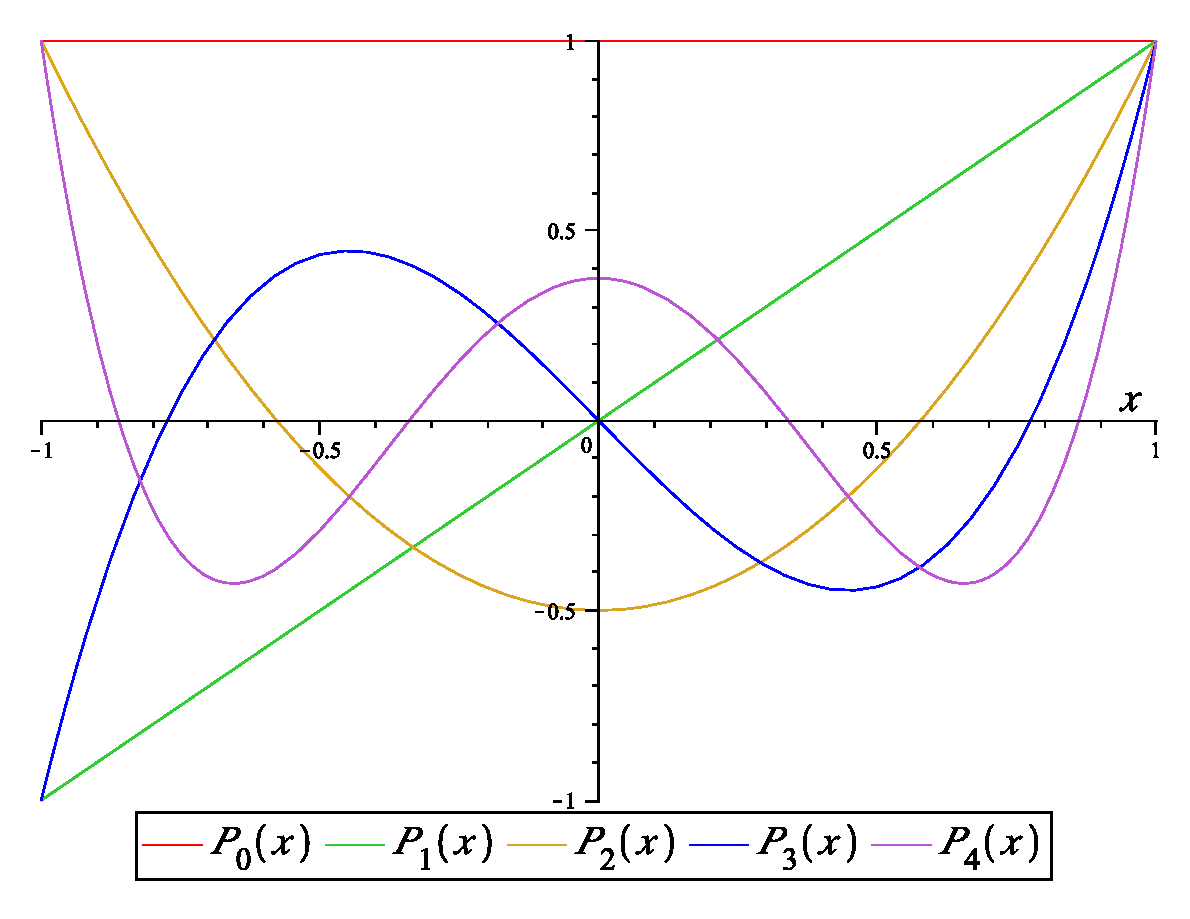
\includegraphics[natheight=7.489300in,natwidth=9.989500in,height=3.3987in,width=4.5238in]
{VOLUMEN_2/02_Series/Figuras/Legendre1.eps}
\caption{Polinomios de Legendre}
\label{poligendre}
\end{center}
\end{figure}
\end{center}
\begin{itemize}
\item  Tienen una representaci�n integral de la forma
\[
P_{n}(x)=\frac1{2\pi}\int_{0}^{\pi}\left[  x+\sqrt{x^{2}-1}\cos\varphi\right]
^{n}\mathrm{d}\varphi
\]
\item  Cambios de variables inmediatos conllevan a ecuaciones diferenciales equivalentes
\begin{itemize}
\item  Forma autoadjunta
\[
\left[  (1-x^{2})\ y^{\prime}\right]  ^{\prime}+\lambda(\lambda+1)\ y=0
\]
\item  En coordenadas esf�ricas con $u=P_{n}(\cos(\theta))$
\[
\frac1{\operatorname*{sen}(\theta)}\frac{\mathrm{d}}{\mathrm{d}\theta}\left(
\operatorname*{sen}(\theta) \frac{\mathrm{d}u}{\mathrm{d}\theta}\right)
+\lambda(\lambda+1)u=0
\]
\item  En coordenadas esf�ricas con $u=\sqrt{\operatorname*{sen}\theta
}P_{n}(\cos\theta)$
\[
\frac{\mathrm{d}^{2}u}{\mathrm{d}\theta^{2}}+\left[  \left(  \lambda
+\frac12\right)  ^{2}+\frac1{4\operatorname*{sen}^{2}(\theta)}\right]  u=0
\]
\end{itemize}
\end{itemize}

\subsection{Potencial Electrost�tico de un Dipolo El�ctrico}

En F�sica el ejemplo claro es el c�lculo del potencial electrost�tico producido por dos cargas $q_{1}=+q$ y $q_{2}=-q$ separadas por una distancia $2d$ en un punto $P$ cualquiera de un plano $\left(  x,y\right)  $. El potencial en ese punto
gen�rico viene dado por
\[
V=q\left(  \frac{1}{R^{\prime}}-\frac{1}{R}\right)
\]
\begin{figure}
[ptb]
\begin{center}
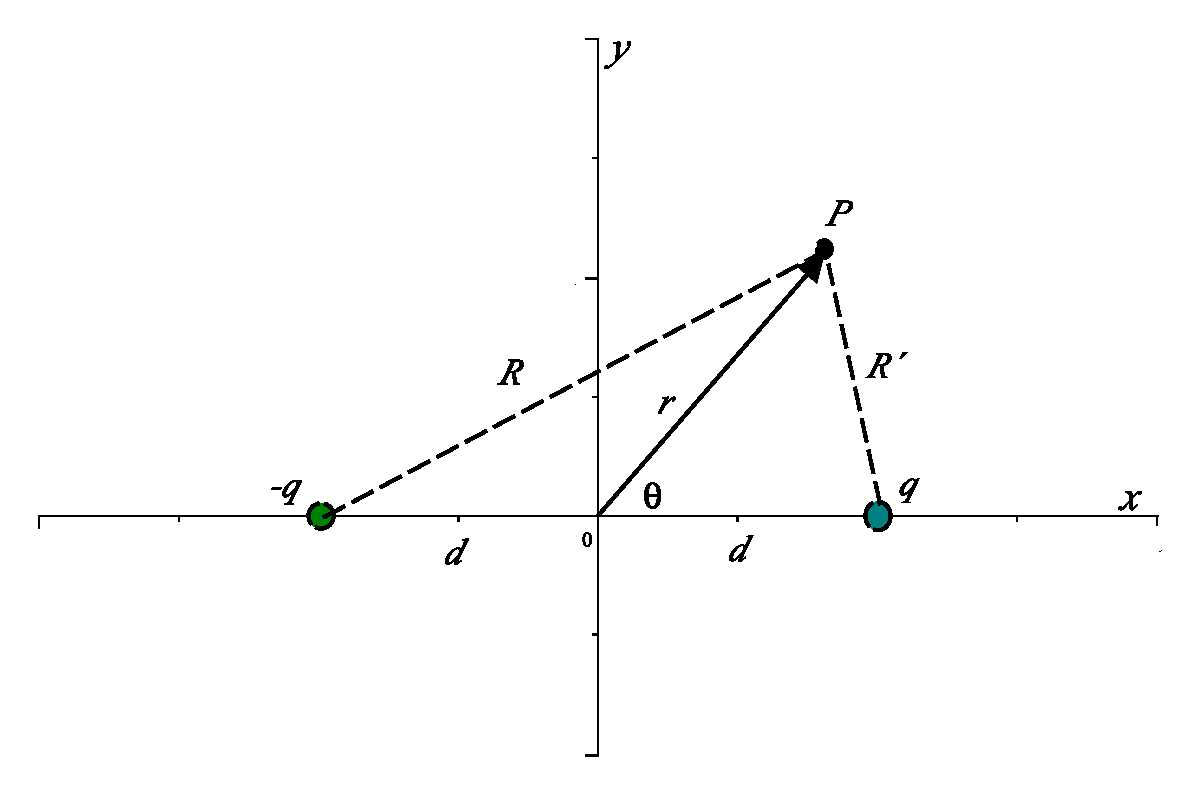
\includegraphics[width=4.0in]{VOLUMEN_2/02_Series/Figuras/Potencial.eps}
\caption{Potencial electrost�tico de un dipolo el�ctrico}
\label{potencial1}
\end{center}
\end{figure}
Tal y como puede apreciarse de la figura \ref{potencial1}
\[
\left(R^{\prime}\right)^{2}=r^{2}+d^{2}-2r\ d\cos(\theta) \quad \mbox{y} \quad
R^{2}=r^{2}+d^{2}-2r\ d\cos\left(\pi-\theta\right)\,,
\]
por lo cual
\begin{align*}
\frac{1}{R^{\prime}}& =\frac{1}{r}\left[1-2 \cos(\theta)\left(\frac{d}{r}\right) +
\left(\frac{d}{r}\right)^{2}  \right]^{-1/2}\\
\frac{1}{R}  & =\frac{1}{r}\left[ 1- 2\cos\left(\pi-\theta\right) 
\left( \frac{d}{r}\right)   +\left( \frac{d}{r}\right)^{2}  \right]^{-1/2}\,
\end{align*}
y consecuentemente
\begin{align*}
\frac{1}{R^{\prime}}  & =\frac{1}{r}\sum_{n=0}^{\infty}
P_{n}(\cos (\theta)) \left(  \frac{d}{r}\right)^{n}\\
\frac{1}{R}  & =\frac{1}{r}\sum_{n=0}^{\infty}
P_{n}\left[ \cos\left(\pi-\theta\right)  \right] \left(\frac{d}{r}\right)^{n}=\frac{1}
{r}\sum_{n=0}^{\infty}P_{n}(-\cos(\theta)) \left(  \frac{d}{r}\right) ^{n}
\end{align*}
El potencial ser�
\[
V=\frac{q}{r}\ \sum_{n=0}^{\infty}\left[ P_{n}(\cos(\theta)) -P_{n}
(-\cos(\theta)) \right]  \left(\frac{d}{r}\right)^{n}
\]
donde todos los t�rminos pares de $P_{n}(\cos(\theta))$ se anulan y finalmente tendremos la expresi�n del potencial para cualquier punto del plano
\[
V=\frac{2q}{r}\ \sum_{n=0}^{\infty}P_{2n+1}(\cos(\theta))\ \left(
\frac{d}{r}\right)^{2n+1}
\]
Nos quedamos con el primer t�rmino de la serie, si
\[
\frac{d}{r}\ll1\quad\Rightarrow\quad V\approx\frac{q}{r^{2}}\ 2d\cos(\theta)\,.
\]

\subsection{Resumen de Propiedades Polinomios Legendre}
%\begin{center}
%\begin{boxedminipage}[h]{16.9cm}
\begin{tabular}{rl} 
Definici�n: &  $P_{n}(x)=\dfrac1{n!2^{n}}\dfrac{\mathrm{d}^{n}}{\mathrm{d}x^{n}}(x^{2}-1)^{n},
\quad n=0,1,2, \dots$ \\ \\
Ejemplos: &  $ P_{0}\equiv1;\quad P_{1}=x; \quad P_{2}=\frac12(3x^{2}-1);\quad P_{3}=\frac12(5x^{3}-3x) $ \\ \\
Relaci�n de Recurrencia: & $\left(  n+1\right)  P_{n+1}(x)=\ \left(2n+1\right)  xP_{n}(x)-nP_{n-1}(x)$ \\ \\
Ecuaciones Diferenciales: & $(1-x^{2})\ y^{\prime\prime}-2x\ y^{\prime}+\lambda(\lambda+1)\ y=0 $\\ \\
 &$\dfrac1{\mbox{sen}(\theta)}\dfrac{\mathrm{d}}{\mathrm{d}\theta}\left(
\mbox{sen}(\theta) \dfrac{\mathrm{d}u}{\mathrm{d}\theta}\right)
+n(n+1)u=0;\quad u=P_{n}(\cos(\theta))$ \\ \\
Funci�n Generatriz:  & $\mathcal{P}(t,x)=\dfrac1{\sqrt{1-2xt+t^{2}}}={\displaystyle\sum_{n=0}^{\infty}}
P_{n}(x)\ t^{n}$ \\ \\
Representaci�n Integral: & $P_{n}(x)=\dfrac1{2\pi}{\displaystyle\int_{0}^{\pi}}
\left[  x+\sqrt{x^{2}-1}\cos\varphi\right]  ^{n}\mathrm{d}\varphi$ \\ \\
Ortogonalidad: & ${\displaystyle\int_{-1}^{1}} P_{\alpha}(x)P_{\beta}(x)\mathrm{d}x=\delta_{\alpha\beta}\dfrac2{2\alpha+1}$
\end{tabular}
%\end{boxedminipage}
%\end{center}

%\begin{center}
%\begin{boxedminipage}[h]{16.9cm}
Practicando con Maple: \\
\textcolor{red}{ $>$ {\tt restart:} } \\
\textcolor{red}{ $>$ {\tt plot([LegendreP(0,x),LegendreP(1,x),LegendreP(2,x),LegendreP(3,x),\\   
 LegendreP(4,x)],x=-1..1);}} 
%\end{boxedminipage}
%\end{center}


\subsection{Polinomios de Hermite}

Los polinomios de Hermite a diferencia de los de Legendre (y Tchevychev), vienen definidos en toda la recta real, vale decir, $x \in (-\infty, \infty)$, por lo cual la funci�n peso $w(x)$ en el producto interno deber� decrecer m�s r�pido que $|x|^{n}$, para garantizar que la norma de los vectores en este espacio vectorial sea finita. La funci�n m�s simple que cumple estos requisitos es $w(x)= e^{-x^{2}} $ (tambi�n algunos autores utilizan $w(x)= e^{-x^{2}/2})$ Esto es, el producto interno entre los polinomios de Hermite vendr� definido como
\[
 \int_{-\infty}^{\infty}\mathrm{d}x \ w(x) f(x)g(x)=  \int_{-\infty}^{\infty}\mathrm{d}x \ e^{-x^{2}} f(x)g(x)\,.
\]
Otra vez, para este producto interno, si ortogonalizamos con Gram-Schmidt se obtienen los polinomios de Hermite. Al igual que el resto de los polinomios ortogonales, existe una f�rmula de Rodrigues para los polinomios de Hermite
\[
H_{n}(x) = (-1)^{n} \ e^{x^{2}} \frac{\mathrm{d}^{n}}{\mathrm{d}x^{n}}e^{-x^{2}}\,,
\]
los cinco primeros polinomios de Hermite son los siguientes:
\begin{align*}
 H_{0}(x) = 1,   						 &  & H_{1}(x) =  2x  				\\
 H_{2}(x) = 4x^{2} - 2,  				     &  & H_{3}(x)  =  8x^{3} -12x,	 \\
 H_{4}(x)= 16x^{4} -48 x^{2} +12	         &  & H_{5}(x) = 32x^{5} -160x^{3} +120 x
\end{align*}

\subsection{Generalidades de los Polinomios de Hemite}
Los polinomios de Hermite ser�n ortogonales, pero no normales
\[
\int_{-\infty}^{\infty}e^{-x^{2}}H_{\beta}(x)H_{\alpha}(x)\mathrm{d}x=2^{\alpha}\alpha!\sqrt{\pi}\ \delta_{\alpha\beta}\,,
\]
por lo tanto:
\[
\int_{-\infty}^{\infty}e^{-x^{2}}H_{\alpha}
^{2}(x)\mathrm{d}x=2^{\alpha} \alpha! \sqrt{\pi}\,.
\]
Donde la funci�n delta de Kronecker es 
$\delta_{\alpha\beta}=0$ si $\alpha\neq\beta$; y $\delta_{\beta\beta}=1.$  

Antes de desarrollar funciones en
t�rminos de los polinomios de Hermite, expondremos un par de teoremas sin
demostraci�n.
%\begin{center}
%\begin{boxedminipage}[h]{16.9cm}
\paragraph{Teorema 1:} Sean $f$ y $g$ dos funciones arbitrarias, cuando menos continuas a trozos en
$\left(  -\infty,\infty\right)  $ y que cumplen con
\[
\int_{-\infty}^{\infty}e^{-x^{2}}f^{2}(x)\mathrm{d}x \quad \exists \quad \wedge
\qquad\int_{-\infty}^{\infty}e^{-x^{2}}g^{2}(x)\mathrm{d} \quad \exists \quad 
\]
Entonces el conjunto de estas funciones forman un espacio vectorial euclideano
$\mathcal{I}_{2}^{w}$ con un producto interno definido por
\[
\int_{-\infty}^{\infty}e^{-x^{2}}f(x)g(x)\mathrm{d}x
\]
Las funciones $f(x)$ y $g(x)$ se denominan cuadrado-integrables respecto al
peso $w$. Es por ello que denotamos el espacio de funciones como
$\mathcal{I}_{2}^{w}$.
%\end{boxedminipage}
%\end{center}

%\begin{center}
%\begin{boxedminipage}[h]{16.9cm}
\paragraph{Teorema 2:}  Si $f(x)$ es una funci�n continua arbitraria en
$\mathcal{I}_{2}^{w}$ entonces puede ser aproximada por un polinomio en ese
mismo espacio. Es decir
\[
\lim_{n\rightarrow\infty}\left|  f(x)-p_{n}(x)\right|  =\lim_{n\rightarrow
\infty}\left(  \int_{-\infty}^{\infty}e^{-x^{2}}\left[  f(x)-p_{n}(x)\right]
^{2}\mathrm{d}x\right)  ^{1/2}=0
\]
%\end{boxedminipage}
%\end{center}


As\'{\i}, la expresi�n de una funci�n arbitraria en la base de los
polinomio de Hermite se reduce a
\[
f(x)=
\sum_{k=0}^{\infty} \frac1{2^{k}k!\sqrt{\pi}}\left[ \int_{-\infty}^{\infty}e^{-t^{2}
}f(t)H_{k}(t)\, \mathrm{d}x\right] \ H_{k}(x)\,,
\]
donde
\[
a_{k}=\frac1{2^{k}k!\sqrt{\pi}} \int_{-\infty}^{\infty}e^{-t^{2}
}f(t)H_{k}(t)\, \mathrm{d}x \,.
\]

\paragraph{Ejemplo:}
Si $f(x)=x^{2}$
\[
f(x)=x^{2}=\sum_{k=0}^{2}b_{k} x^k = \sum_{k=0}^{\infty}a_{k}\ H_{k}(x)
\]
\begin{eqnarray*}
f(x)=x^{2}&=& a_0 H_0(x)+a_1 H_1(x)+a_2 H_2(x)\\
&=& a_0+a_1(2x)+a_2(4x^2-1)\\
&=& (a_0-a_2) + 2 a_1 x + 4a_2 x^2 \,\,\, \Rightarrow a_0=\frac14\,, a_1=0\,, a_2=\frac14\,.\\
&=& \frac14 H_0(x)+\frac14  H_2(x)\,
\end{eqnarray*}

Si generalizamos para funciones del tipo  $f(x)=x^{2p}$ con $p=1,2,3,\cdots$, entonces 
\[
f(x)=x^{2p}=\sum_{k=0}^{2p}b_{k} x^k = \sum_{k=0}^{\infty}a_{2k}\ H_{2k}(x)\,,
\]
por lo tanto
\[
a_{2k} =\frac1{2^{2k}(2k)!\sqrt{\pi}}\int_{-\infty}^{\infty}e^{-x^{2}
}x^{2p}H_{2k}(x)\mathrm{d}x = \frac1{2^{2k}(2k)!\sqrt{\pi}}\int_{-\infty}^{\infty}x^{2p}\frac
{\mathrm{d}^{2k}}{\mathrm{d}x^{2k}}e^{-x^{2}}\mathrm{d}x\,.
\]

Una integraci�n por partes estrat�gica muestra que:
\[
a_{2k}=\frac1{2^{2k}(2k)!\sqrt{\pi}}\left\{  \left.  x^{2p}\frac
{\mathrm{d}^{2k-1}}{\mathrm{d}x^{2k-1}}e^{-x^{2}}\right|  _{-\infty}^{\infty
}-\int_{-\infty}^{\infty}2px^{2p-1}\frac{\mathrm{d}^{2k-1}}{\mathrm{d}
x^{2k-1}}e^{-x^{2}}\mathrm{d}x\right\}\,.
\]
El primer t�rmino de la resta se anula debido a la definici�n de
los polinomios de Hermite
\[
\left.  x^{2p}\frac{\mathrm{d}^{2k-1}}{\mathrm{d}x^{2k-1}}e^{-x^{2}}\right|
_{-\infty}^{\infty}=\left.  x^{2p}(-1)^{2k-1}e^{-x^{2}}H_{2k-1}(x)\right|
_{-\infty}^{\infty}\,.
\]

Repitiendo el proceso $2k$ veces, tendremos
\[
a_{2k}=\frac1{2^{2k}(2k)!\sqrt{\pi}}\frac{\left(  2p\right)  !}{\left(
2p-2k\right)  !}\int_{-\infty}^{\infty}x^{2p-2k}\ e^{-x^{2}}\mathrm{d}x
\]
si en la integral hacemos $x=\sqrt{t}$ obtenemos
\begin{align*}
a_{2k}  & =\frac1{2^{2k}(2k)!\sqrt{\pi}}\frac{\left(  2p\right)  !}{\left(
2p-2k\right)  !}\int_{-\infty}^{\infty}t^{p-k}\ e^{-t}\frac{\mathrm{d}%
t}{2\sqrt{t}}\\
& =\frac1{2^{2k+1}(2k)!\sqrt{\pi}}\frac{\left(  2p\right)  !}{\left(
2p-2k\right)  !}\int_{-\infty}^{\infty}t^{p-k-\frac12}\ e^{-t}\mathrm{d}t
\end{align*}
y utilizando la definici�n $\Gamma\left(  z\right)  \equiv\int_{0}%
^{\infty}e^{-t}t^{z-1}\mathrm{d}t\equiv\left(  z-1\right)  !$ , queda como
\[
a_{2k}=\frac1{2^{2k+1}(2k)!\sqrt{\pi}}\frac{\left(  2p\right)  !}{\left(
2p-2k\right)  !}\Gamma\left(  p-k+\frac12\right)\,.
\]

Ahora, recurrimos a la propiedad de ``duplicaci�n'' de la Funci�n
Gamma, i.e.
\[
2^{2z-1}\Gamma\left(  z\right)  \Gamma\left(  z+\frac12\right)  =\sqrt{\pi
}\Gamma\left(  2z\right)
\]
tenemos que
\[
2^{2p-2k}\Gamma\left(  p-k+\frac12\right)  \left(  p-k\right)  !=\sqrt{\pi
}\left(  2p-2k\right)  !
\]
quedan entonces los coeficientes determinados como
\[
a_{2k}=\frac{\left(  2p\right)  !}{2^{2p+1}(2k)!\left(  p-k\right)  !}
\]
y, por lo tanto el desarrollo en la base de los polinomios de Hermite
\[
f(x)=x^{2p}=\frac{\left(  2p\right)  !}{2^{2p+1}}\sum_{k=0}^{p}\ \frac
{H_{2k}(x)}{(2k)!\left(  p-k\right)  !}\qquad-\infty<x<\infty\,.
\]

Muestre que del mismo modo se puede encontrar
\[
f(x)=x^{2p+1}=\frac{\left(  2p-1\right)  !}{2^{2p-1}}\sum_{k=0}^{p}%
\ \frac{H_{2k+1}(x)}{(2k+1)!\left(  p-k\right)  !}\qquad-\infty<x<\infty\,.
\]

Si $f(x)=e^{-a^{2}x^{2}}$ con $\operatorname{Re}a^{2}>-1.$ Otra vez
\[
f(x)=e^{-a^{2}x^{2}}=\sum_{k=0}^{\infty}a_{2k}\ H_{2k}(x)
\]
entonces
\begin{equation}
a_{2k}=\frac1{2^{2k}(2k)!\sqrt{\pi}}\int_{-\infty}^{\infty}e^{-(a^{2}+1)x^{2}%
}H_{2k}(x)\mathrm{d}x\nonumber
\end{equation}
Sustituyendo $H_{2k}(x)$ por su expresi�n integral tendremos
\begin{align*}
a_{2k}  & =\frac1{2^{2k}(2k)!\sqrt{\pi}}\int_{-\infty}^{\infty}e^{-(a^{2}%
+1)x^{2}}\left[  \frac{2^{2k+1}(-1)^{k}e^{x^{2}}}{\sqrt{\pi}}\int_{0}^{\infty
}e^{-t^{2}}t^{2k}\cos2xt\ \mathrm{d}t\right]  \mathrm{d}x\\
& =\frac{2(-1)^{k}}{\pi(2k)!}\int_{-\infty}^{\infty}e^{-a^{2}x^{2}}\left[
\int_{0}^{\infty}e^{-t^{2}}t^{2k}\cos2xt\ \mathrm{d}t\right]  \mathrm{d}x\\
& \equiv\frac{2(-1)^{k}}{\pi(2k)!}\int_{0}^{\infty}e^{-t^{2}}t^{2k}\left[
\int_{-\infty}^{\infty}e^{-a^{2}x^{2}}\cos2xt\ \mathrm{d}x\right]
\ \mathrm{d}t\\
& =\frac{2(-1)^{k}}{\pi(2k)!}\int_{0}^{\infty}e^{-t^{2}}t^{2k}\left[
\sqrt{\frac\pi{a^{2}}}\ e^{-t^{2}/a^{2}}\right]  \ \mathrm{d}t=\\
& =\frac{2(-1)^{k}}{\sqrt{\pi}(2k)!a}\int_{0}^{\infty}e^{-t^{2}(1+a^{-2}%
)}\ t^{2k}\ \mathrm{d}t\\
& =\frac{(-1)^{k}}{\sqrt{\pi}(2k)!}\ \frac{a^{2k}}{\left(  1+a^{2}\right)
^{k+1/2}}\int_{0}^{\infty}e^{-s}\ s^{k-\frac12}\ \mathrm{d}s\qquad\leftarrow
t^{2}(1+a^{-2})=s\\
& =\frac{(-1)^{k}}{\sqrt{\pi}(2k)!}\ \frac{a^{2k}}{\left(  1+a^{2}\right)
^{k+1/2}}\Gamma\left(  k+\frac12\right)
\end{align*}
y ahora usando, otra vez la propiedad de ``duplicaci�n'' de la funci�n
gamma,
\[
2^{2k}\Gamma\left(  k+\frac12\right)  k!=\sqrt{\pi}\left(  2k\right)  !
\]
obtenemos
\[
a_{2k}=\frac{(-1)^{k}a^{2k}}{2^{2k}\ k!\left(  1+a^{2}\right)  ^{k+1/2}}\
\]
por lo tanto
\[
f(x)=e^{-a^{2}x^{2}}=\sum_{k=0}^{\infty}\frac{(-1)^{k}a^{2k}}{2^{2k}%
\ k!\left(  1+a^{2}\right)  ^{k+1/2}}\ H_{2k}(x)
\]

Al igual que los polinomios de Legendre, los de Hermite, surgen tambi�n en sus or�genes como soluciones a la ecuaci�n diferencial ordinaria del tipo 
\[
 \frac{\mathrm{d}^2 H_{n}(x)}{\mathrm{d} x^2} -2x \ \frac{\mathrm{d} H_{n}(x)}{\mathrm{d} x} + nH_{n}(x) =0
\]
Vale decir:
\begin{center}
\begin{tabular}{cll}
$n$ & Ecuaci�n de Hermite & Soluci�n \\ \hline \hline\\
0 & $ \dfrac{\mathrm{d}^2 H_{0}(x)}{\mathrm{d} x^2} -2x \dfrac{\mathrm{d} H_{0}(x)}{\mathrm{d} x}=0$  &$ H_{0}(x)=1$ \\ \\
1 & $ \dfrac{\mathrm{d}^2 H_{1}(x)}{\mathrm{d} x^2} -2x \dfrac{\mathrm{d} H_{1}(x)}{\mathrm{d} x}+ 2 H_{1}(x)=0$ & $H_{1}(x) = 2x $ \\ \\
2 & $ \dfrac{\mathrm{d}^2 H_{2}(x)}{\mathrm{d} x^2} -2x \dfrac{\mathrm{d} H_{2}(x)}{\mathrm{d} x} + 4 H_{2}(x)=0$ & $H_{2}(x)=4x^{2} -2$ \\ \\
3 & $ \dfrac{\mathrm{d}^2 H_{3}(x)}{\mathrm{d} x^2} -2x \dfrac{\mathrm{d} H_{3}(x)}{\mathrm{d} x} + 6 H_{3}(x) = 0$ & $H_{3}(x)= 8x^{3} -12x $ \\ \\
4& $ \dfrac{\mathrm{d}^2 H_{4}(x)}{\mathrm{d} x^2} -2x \dfrac{\mathrm{d} H_{4}(x)}{\mathrm{d} x} + 8 H_{4}(x)=0$ & $H_{4}(x)=16 x^{4} -48x^{2} +12$  \\\\
\hline \hline
\end{tabular}
\end{center}

\subsection{Funci�n Generatriz de los Polinomios de Hermite}

Se puede encontrar una funci�n generatriz $\mathcal{H}(t,x)$ de los polinomios de Hermite:
\[
\mathcal{H}(t,x)=e^{2xt-t^{2}}=H_{0}(x)\ +H_{1}(x)\ t+\frac{H_{2}(x)}
2\ t^{2}+\frac{H_{3}(x)}{3!}\ t^{2}+\cdots=\sum_{n=0}^{\infty}\frac{H_{n}
(x)}{n!}\ t^{n}
\]
para la cual los $H_{n}(x)$ son los coeficientes de su desarrollo en series de
potencias. Es f�cil darse cuenta que esta expresi�n proviene del
desarrollo en Serie de Taylor
\[
\mathcal{H}(t,x)=e^{2xt-t^{2}}=\sum_{n=0}^{\infty}\frac1{n!}\left[
\frac{\partial^{n}\mathcal{H}(t,x)}{\partial t^{n}}\right]  _{t=0}
\ t^{n}\qquad\left\|  t\right\|  <\infty
\]
para lo cual
\[
\left[  \frac{\partial^{n}\mathcal{H}(t,x)}{\partial t^{n}}\right]
_{t=0}=e^{x^{2}}\left[  \frac{\partial^{n}}{\partial t^{n}}e^{-\left(
x-t\right)  ^{2}}\right]  _{t=0}=\left(  -1\right)  ^{n}e^{x^{2}}\left[
\frac{\mathrm{d}^{n}}{\mathrm{d}u^{n}}e^{-\left(  u\right)  ^{2}}\right]
_{u=x}=H_{n}(x)
\]
\subsection{Relaci�n de Recurrencia}

A partir de la funci�n generatriz se puede construir la siguiente identidad
\[
\frac{\partial\mathcal{H}(t,x)}{\partial t}=\left(2x-2t\right)  \mathcal{H}
\]
y utilizando el desarrollo en series de potencias en $t$ tendremos,
\begin{eqnarray*}
\sum_{n=1}^{\infty}\frac{H_{n}(x)}{n!} nt^{n-1} &=& 2x\sum_{n=0}^{\infty}
\frac{H_{n}(x)}{n!}\ t^{n}-\sum_{n=0}^{\infty}\frac{H_{n}(x)}{n!}\ t^{n+1}\,, \\
\sum_{n=1}^{\infty}\frac{H_{n}(x)}{n!} nt^{n-1} &-& 2x\sum_{n=0}^{\infty}
\frac{H_{n}(x)}{n!}\ t^{n}+\sum_{n=0}^{\infty}\frac{H_{n}(x)}{n!}\ t^{n+1}=0\,,\\
\sum_{n=0}^{\infty}\frac{H_{n+1}(x)}{(n+1)!} (n+1)t^{n} &-& 2x\sum_{n=0}^{\infty}
\frac{H_{n}(x)}{n!}\ t^{n}+\sum_{n=1}^{\infty}\frac{H_{n-1}(x)}{(n-1)!}\ t^{n}=0\,,\\
H_1(x)+\sum_{n=1}^{\infty}\frac{H_{n+1}(x)}{(n+1)!} (n+1)t^{n} &-& 2x H_0(x) -2x\sum_{n=1}^{\infty}
\frac{H_{n}(x)}{n!}\ t^{n}+\sum_{n=1}^{\infty}\frac{H_{n-1}(x)}{(n-1)!} t^{n}=0\,,\\
\underbrace{H_1(x)-2x H_0(x)}_{=0} &+& \sum_{n=1}^{\infty}\left[ \frac{H_{n+1}(x)}{(n+1)!} (n+1)
 -2x \frac{H_{n}(x)}{n!} +\frac{H_{n-1}(x)}{(n-1)!}\right]t^n=0\,,
\end{eqnarray*}
es decir:
\[
\sum_{n=1}^{\infty} 
\left[\underbrace{ \frac{H_{n+1}(x)}{(n+1)!} (n+1) -2x
\frac{H_{n}(x)}{n!}+\frac{H_{n-1}(x)}{(n-1)!} }_{=0}\right] t^{n}  =0\,.
\]
Por lo tanto:
\[
\frac{H_{n+1}(x)}{n!} -2x\frac{H_{n}(x)}{n!}+\frac{H_{n-1}(x)}{(n-1)!}=0
\]
As\'{\i} la relaci�n de recurrencia ser�
\[
H_{n+1}(x)-2xH_{n}(x)+2nH_{n-1}(x)=0
\]
De igual modo, podemos partir de otra identidad
\[
\frac{\partial\mathcal{H}(t,x)}{\partial x}=2t\ \mathcal{H}\Rightarrow
\sum_{n=0}^{\infty}\frac{H_{n}^{\prime}(x)}{n!}\ t^{n}=2\sum_{n=0}^
{\infty}\frac{H_{n}(x)}{n!}\ t^{n+1}\,,
\]
es decir:
\[
\sum_{n=1}^{\infty}\frac{H_{n}^{\prime}(x)}{n!}\ t^{n}=
2\sum_{n=1}^{\infty}\frac{H_{n-1}(x)}{(n-1)!}\ t^{n}\,\Rightarrow
\frac{H_{n}^{\prime}(x)}{n!} =2\frac{H_{n-1}(x)}{(n-1)!}
\]
y encontrar una relaci�n para generar las derivadas de los polinomios de Hermite en 
t�rmino de ellos mismos:
\[
H_{n}^{\prime}(x)=2n\ H_{n-1}(x),\qquad n=1,2,3,\cdots\,.
\]

Finalmente, utilizando la ecuaci�n anterior en la relaci�n de
recurrencia y derivando esa expresi�n una vez m�s, queda como:
\begin{align*}
H_{n+1}(x)-2xH_{n}(x)+H_{n}^{\prime}(x)  & =0\\
H_{n}^{\prime\prime}(x)-2xH_{n}^{\prime}(x)+2n\ H_{n}(x)  & =0
\end{align*}
con lo cual queda demostrado que los polinomios de Hermite son una soluci�n particular 
de esa ecuaci�n diferencial.
\[
y^{\prime\prime}-2xy^{\prime}+2ny=0,
\]
Donde hemos hecho $y=H_{n}(x)$ Adicionalmente, podremos demostrar 
que $y=e^{-x^{2}/2}H_{n}(x)$ es soluci�n de la ecuaci�n diferencial autoadjunta
\[
y^{\prime\prime}+\left(  2n+1-x^{2}\right)  y=0 \,.
\]
\subsection{Ortogonalidad y Norma de los Polinomios de Hermite}
En general
estos polinomios cumplen con
\[
\int_{-\infty}^{\infty}e^{-x^{2}}H_{\beta}(x)H_{\alpha}(x)\mathrm{d}x = 
2^{\alpha}\alpha!\sqrt{\pi} \delta_{\alpha\beta}\,.
\]
Donde la funci�n delta de Kronecker es $\delta_{\alpha\beta}=0$ si
$\alpha\neq\beta$; y $\delta_{\beta\beta}=1$.
Para demostrar el caso $\alpha\neq\beta$ partimos de
\begin{align*}
u_{\beta}\left[  u_{\alpha}^{\prime\prime}+\left(  2\alpha+1-x^{2}\right)
u_{\alpha}\right]   & =0\\
u_{\alpha}\left[  u_{\beta}^{\prime\prime}+\left(  2\beta+1-x^{2}\right)
u_{\beta}\right]   & =0
\end{align*}
restando miembro a miembro e integrando se tiene que:
\begin{align*}
\left[  u_{\alpha}^{\prime}u_{\beta}-u_{\beta}^{\prime}u_{\alpha}\right]
^{\prime}+2\left(  \alpha-\beta\right)  u_{\alpha}u_{\beta} & =0\\
\left(  \alpha-\beta\right)  \int_{-\infty}^{\infty}e^{-x^{2}}H_{\alpha
}(x)H_{\beta}(x)\mathrm{d}x  & =0\\
\int_{-\infty}^{\infty}e^{-x^{2}}H_{\alpha}(x)H_{\beta}(x)\mathrm{d}x  &
=0\qquad\alpha\neq\beta;
\end{align*}
ya que
\[
\left.  e^{-x^{2}/2}\left\{  2\alpha\ H_{\alpha-1}(x)H_{\beta}(x)-2\beta
\ H_{\beta-1}(x)H_{\alpha}(x)\right\}  \right|  _{-\infty}^{\infty}=0
\]
Para encontrar el valor de la norma, procedemos a partir de la relaci�n de
recurrencia
\begin{align*}
H_{n}(x)\left[  H_{n}(x)-2xH_{n-1}(x)+2(n-1)H_{n-2}(x)\right]   & =0\\
H_{n-1}(x)\left[  H_{n+1}(x)-2xH_{n}(x)+2nH_{n-1}(x)\right]   & =0
\end{align*}
restando miembro a miembro, multiplicando por $e^{-x^{2}}$ e integrando entre
$(-\infty,\infty)$ se obtiene
\[
\int_{-\infty}^{\infty}e^{-x^{2}}H_{\alpha}^{2}(x)\mathrm{d}x=2\alpha
\int_{-\infty}^{\infty}e^{-x^{2}}H_{\alpha-1}^{2}(x)\mathrm{d}x
\]
repitiendo la operaci�n y recordando que al final queda
\[
\int_{-\infty}^{\infty}e^{-x^{2}}x^{2}\mathrm{d}x=2\sqrt{\pi}
\]
Obtenemos
\[
\int_{-\infty}^{\infty}e^{-x^{2}}H_{\alpha}
^{2}(x)\mathrm{d}x=2^{\alpha}\alpha!\sqrt{\pi}
\]
\subsection{Representaci�n Integral de los Polinomios de Hermite}
 Los
polinomios de Hermite pueden ser representados como
\[
H_{n}(x)=\frac{2^{n}(-i)^{n}e^{x^{2}}}{\sqrt{\pi}}\int_{-\infty}^{\infty
}e^{-t^{2}+2itx}t^{n}\mathrm{d}t
\]
que puede ser separada como
\[
H_{2n}(x)=\frac{2^{2n+1}(-1)^{n}e^{x^{2}}}{\sqrt{\pi}}\int_{0}^{\infty
}e^{-t^{2}}t^{2n}\cos(2xt) \mathrm{d}t\,,\quad n=1,2,3,\cdots
\]
y para los t�rminos impares
\[
H_{2n+1}(x)=\frac{2^{2n+2}(-1)^{n}e^{x^{2}}}{\sqrt{\pi}}\int_{0}^{\infty
}e^{-t^{2}}t^{2n+1}\mbox{sen}(2xt) \mathrm{d}t \,, \quad n=1,2,3,\cdots
\]
La forma de llegar a cualquiera de estas �ltimas f�rmulas se parte de
las conocidas integrales desarrolladas en el plano complejo
\[
e^{-x^{2}}=\frac2{\sqrt{\pi}}\int_{-\infty}^{\infty}e^{-t^{2}}\cos(2xt) \mathrm{d}t
\]
se deriva $2n$ veces a ambos miembros se utiliza la definici�n de los
polinomios de Hermite.

\begin{center}
\begin{figure}
[ptb]
\begin{center}
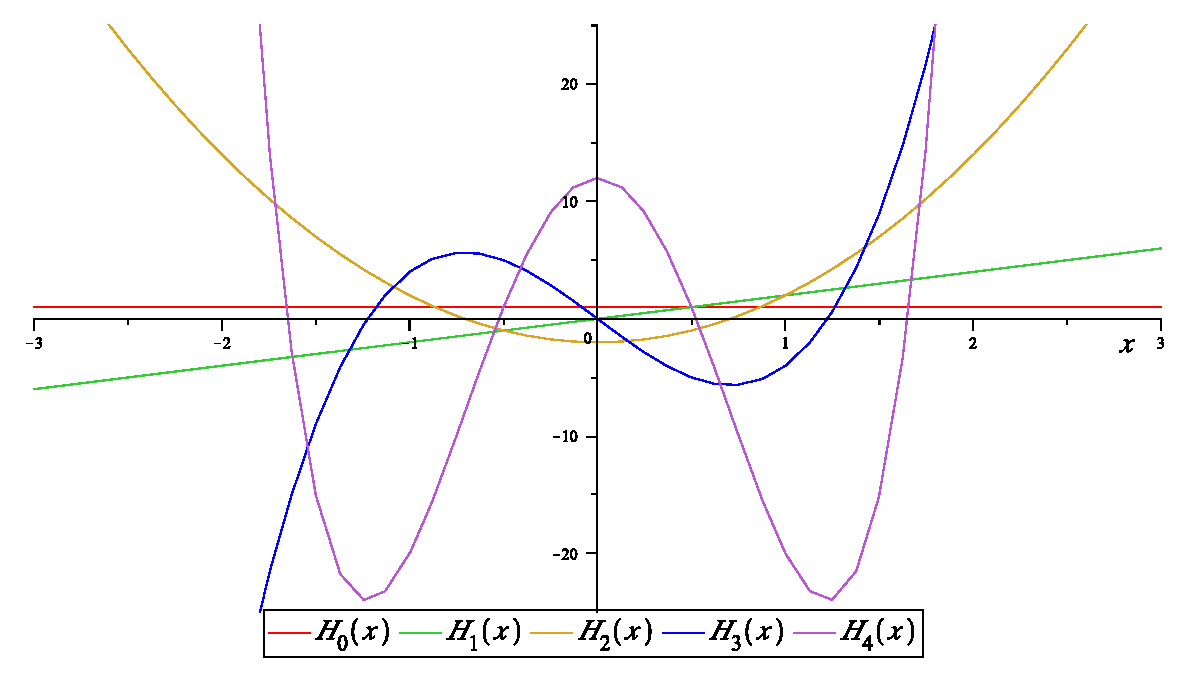
\includegraphics[width=4.8in]{VOLUMEN_2/02_Series/Figuras/hermite.eps}
\caption{Polinomios de Hermite}
\end{center}
\end{figure}
\end{center}
\subsection{El Oscilador arm�nico, independiente del tiempo, en Mec�nica Cu�ntica.}

La Ecuaci�n de Schr\"{o}dinger independiente del tiempo y en una
dimensi�n es
\[
\frac{\mathrm{d}^{2}}{\mathrm{d}x^{2}}\psi(x)+\frac{2\mu}{\hbar^{2}}
\left[E-\mathcal{U}(x)\right]  \psi(x)=0\,,
\]
con $\mu$ la ``masa'' de la part�cula;$\ E$ los niveles de energ�a y
$\mathcal{U}(x)$ el potencial al cual est� sometida la part�cula. En
el caso que estudiemos un potencial del tipo $\mathcal{U}(x)=\frac{1}{2}\mu\omega
^{2}x^{2}$ en el cual la frecuencia angular del oscilador viene representada
por $\omega$. La ecuaci�n de Schr\"{o}dinger se convierte en
\[
\frac{\mathrm{d}^{2}}{\mathrm{d}x^{2}}\psi(x)+\frac{2\mu}{\hbar^{2}}\left[
E-\frac{1}{2}\mu\omega^{2}x^{2}\right]  \psi(x)=0\,,
\]
haciendo un cambio de variable $\xi=x\sqrt{\mu\omega/\hbar}$ para
adimensionalizar la ecuaci�n de Schr\"{o}dinger, se obtiene
\[
\psi^{\prime\prime}(\xi)+\left[  \frac{2E}{\hbar\omega}-\xi^{2}\right]\psi(\xi)=0\,,
\]
la cual corresponde a la forma autoadjunta de la Ecuaci�n de Hermite:
\[
\psi^{\prime\prime}(\xi)+\left[2n+1-\xi^{2}\right]\psi(\xi)=0\,,
\]
y por lo tanto identificamos
\[
\frac{2E}{\hbar\omega}=2n+1\quad\Rightarrow\quad E=\left(n+\frac{1}
{2}\right)  \hbar\omega\,,
\]
con lo cual comprobamos la forma como viene cuantizada la energ�a en este
sistema y la energ�a del estado fundamental. Por su parte, la funci�n
de onda se podr� expresar en la base de soluciones de esa ecuaci�n
\[
\psi(\xi)=\sum_{n=0}^{\infty}c_{n}\ \psi_{n}(\xi)=\sum_{n=0}^{\infty}
c_{n}\ e^{-\xi^{2}/2}H_{n}(\xi)\,.
\]
Si mantenemos la normalizaci�n
\[
\int_{-\infty}^{\infty}\psi_{n}^{2}(\xi)\mathrm{d}\xi=1 \qquad 
\text{con }c_{n}=\left(\frac{\mu\omega}{\pi\hbar}\right)^{1/4}\frac{1}{\sqrt{2^{n}n!}}\,.
\]

\subsection{Resumen de Propiedades Polinomios Hermite}
%\begin{center}
%\begin{boxedminipage}[h]{16.9cm}
\begin{tabular}{rl} 
Definici�n: &  $H_{n}(x)=(-1)^{n}e^{x^{2}}\dfrac{\mathrm{d}^{n}}{\mathrm{d}x^{n}}e^{-x^{2}},\qquad n=0,1,2, \dots$ \\ \\
& $H_{n}(x)={\displaystyle\sum_{k=0}^{n/2}} \dfrac{(-1)^{k}n!}{k!\left(  n-2k\right)  !}\left(  2x\right)  ^{n-2k} $ \\ \\
Ejemplos: &  $H_{0}(x)=1;\,\, H_{1}(x)=2x; \,\, H_{2}(x)=4x^{2}-2; \,\, H_{3}(x)=8x^{3}-12x$ \\ \\
Relaciones de Recurrencia: & $H_{0}(x)=1;\qquad H_{1}(x)=2x;\qquad H_{2}(x)=4x^{2}-2 $\\ \\
 &  $H_{n}^{\prime}(x)=2n\ H_{n-1}(x),\qquad n=1,2,3,\dots $\\ \\ 
Ecuaciones Diferenciales: & $y^{\prime\prime}-2xy^{\prime}+2ny=0 $ \\ \\
  & $u^{\prime\prime}+\left(  2n+1-x^{2}\right)  u=0;\quad u(x)=e^{-x^{2}/2}H_{n}(x)$  \\ \\
Funci�n Generatriz:  & $\mathcal{H}(t,x)=\mathbf{e}^{2xt-t^{2}}={\displaystyle\sum_{n=0}^{\infty}}
\dfrac{H_{n}(x)}{n!}\ t^{n}$ \\ \\
Representaci�n Integral: &$H_{2n}(x)=\dfrac{2^{2n+1}(-1)^{n}e^{x^{2}}}{\sqrt{\pi}}
{\displaystyle\int_{0}^{\infty}}e^{-t^{2}}t^{2n}\cos(2xt)\ \mathrm{d}t $  \\ \\
   &$H_{2n+1}(x)=\dfrac{2^{2n+2}(-1)^{n}e^{x^{2}}}{\sqrt{\pi}}
{\displaystyle\int_{0}^{\infty}}e^{-t^{2}}t^{2n+1}\mbox{sen}(2xt)\ \mathrm{d}t $ \\ \\
Ortogonalidad: & $2^{\alpha}\alpha!\sqrt{\pi}\ \delta_{\alpha\beta}=
{\displaystyle\int_{-\infty}^{\infty}} e^{-x^{2}}H_{\beta}(x)H_{\alpha}(x)\mathrm{d}x$
\end{tabular}
%\end{boxedminipage}
%\end{center}

%\begin{center}
%\begin{boxedminipage}[h]{16.9cm}
Practicando con Maple: \\
\textcolor{red}{ $>$ {\tt restart: with(orthopoly):} } \\
\textcolor{red}{ $>$ {\tt plot([H(0,x), H(1,x), H(2,x), H(3,x), H(4,x)], x=-3..3,y=-25..25);}} 
%\end{boxedminipage}
%\end{center}

\subsection{{\color{Fuchsia}Ejemplos}}

\subsection{{\color{red}Practicando con Maxima}}

\subsection{{\color{OliveGreen}Ejercicios}}

\section{Planteamiento General para Polinomios Ortogonales}

Hemos considerado un par de ejemplos de Polinomios Ortogonales. En ambos podemos idenficar algunas caracter�sticas comunes. En base a estas caracter�sticas comunes definiremos otras familias de polinomios ortogonales.

\begin{table}[h]
\centering
\begin{tabular}{|c|c|c|c|c|c|c|} \hline
\textbf{Nomenclatura} & \textbf{Nombre} 	& $a$ & $b$ & $w(x)$ & $h_{n}$ & $h_{0}$ \\ \hline \hline 
$P_{n}(x)$ 	& Legendre 		& $-1$ 	& $1$ 	& $1$ 		& $\dfrac{2}{2n +1}$ &  \\\hline 
$T_{n}(x)$ 	& Tchebychev 1E 	& $-1$ 	& $1$ 	& $\dfrac{1}{\sqrt{1 -x^{2}}}$ & $\dfrac{\pi}{2}$ & $\pi$ \\\hline 
$U_{n}(x)$ 	& Tchebychev 2E 	& $-1$ 	& $1$ 	& $\sqrt{1 -x^{2}}$ & $\dfrac{\pi}{2}$ &  \\\hline 
$H_{n}(x)$ 	& Hermite 		& $-\infty$& $\infty$ & $e^{-x^{2}}$ & $2^{n}n! \sqrt{\pi}$ &  \\\hline 
$L_{n}(x)$ 	& Laguerre 		& $0$ 	& $\infty$& $e^{-x}$ & $1$ &  \\\hline 
$L_{n}^{\alpha}(x)$ & Laguerre G 	& $0$ 	& $\infty$ & $x^{\alpha}e^{-x}$ con $\alpha > -1$ & 
	$\frac{\Gamma(n + \alpha +1) }{n!}$ &  \\\hline 
$P_{n}^{\alpha \beta}(x)$ & Jacobi & $-1$ 	& $1$ & $(1-x)^{\alpha} (1+x)^{\beta}$ & \dag & \\ \hline \hline
\end{tabular} 
\caption{Propiedades gen�ricas de los Polinomios Ortogonales, $N_{n}$ indica la norma del 
polinomio de grado $n$.
\label{PropiedadesGenericas}}
\end{table}
$\dag $ En el caso de los polinomios de Jacobi, la norma es 
\[
h_{n} = \frac{2^{\alpha + \beta +1}}{2n + \alpha + \beta +1} 
\frac{ \Gamma(n + \alpha  +1) \Gamma(n +  \beta +1)}{n! \Gamma(n + \alpha + \beta +1) } 
\quad \mbox{con} \quad \alpha > -1 \quad \mbox {y} \quad \beta > -1 \,.
\]

\subsection{Producto interno gen�rico, norma y ortogonalidad}
Los polinomios ortogonales se definen como un conjunto de polinomios $\{ p_{n}(x) \}$ de orden $n$ definidos en un determinado intervalo $a \leq x \leq b$, los cuales son ortogonales respecto a una definici�n de producto interno 
\[
\int_{a}^{b} w(x) p_{m}(x) p_{n}(x)\mathrm{d}x = h_{n} \delta_{nm} \quad \text{con } w(x) > 0 \text{ una funci�n peso en } a \leq x \leq b
\] que garantiza que la norma sea finita en ese intervalo. Dado que el Teorema de Weierstrass garantiza que el conjunto de polinomios  $\{ 1, x, x^2, \cdots, x^n, \cdots \}$ es una base completa para un espacio vectorial $\mathbb{E}^{\infty}$, se procede a ortogonalizar esa base con la definici�n de producto interno y el intervalo que corresponda. Para cada caso tendremos una base ortogonal de polinomios. 
\begin{table}[h]
  \centering 
  \begin{tabular}{|c|c|c|c|} \hline \hline
% after \\ : \hline or \cline{col1-col2} \cline{col3-col4} ...
  \textbf{Polinomio} 	& $\mu_{n}$ 													   & $w(x)$ 				& $q(x)$ \\  \hline \hline
  $P_{n}$ 			& $ 2^{n}n!  $ 											   & $1$					&$1 -x^{2}$  \\  \hline  
  $T_{n}$ 			& $\dfrac{(-1)^{n}}{\sqrt{\pi}} 2^{n+1} \Gamma \left(n + \frac{1}{2} \right)$ 	   & $\dfrac{1}{\sqrt{1 -x^{2}}}$ & $1 -x^{2}$  \\  \hline 
  $U_{n}$ 			& $\dfrac{(-1)^{n}}{(n+1)\sqrt{\pi}} 2^{n+1} \Gamma \left(n + \frac{3}{2} \right) $ &$ \sqrt{1 -x^{2}}$ 			&$1 -x^{2}$  \\  \hline
  $H_{n}$ 			& $(-1)^{n}$ 													   &$e^{-x^{2}} $ 			&$1$ \\  \hline 
  $L_{n}$ 			& $n!$ 														   & $e^{-x} $ 				&$x$ \\  \hline 
  $L_{n}^{\alpha}$ 	& $n!$ 														   & $x^{\alpha}e^{-x} $ 	& $x$\\  \hline 
\hline
\end{tabular}
  \caption{Funciones para determinar la F�rmula de Rodrigues generalizada } 
  \label{FormulaRodrigues}
\end{table}

En el cuadro \ref{PropiedadesGenericas} resumimos las propiedades m�s resaltantes, com lo son: la funci�n peso en el producto interno, el intervalo en el cual est�n definidas estas fuciones y su norma.
\subsection{F�rmula de Rodrigues genelarizada}
En general todos los polinomios ortogonales $\{ p_{n}(x) \}$ vienen definidos por la f�rmula de Rodrigues generalizada 
\[
p_{n}(x)= \dfrac{1}{w(x) \mu_{n}}  \dfrac{\mathrm{d}^{n} }{\mathrm{d}x^{n} } \left( w(x) q(x)^{n} \right)
\]
donde $w(x), q(x)$ y $ \mu_{n}$ vienen especficados en el cuadro \ref{FormulaRodrigues} para cada conjunto de polinomios ortogonales

\subsection{Ejemplos de Polinomios Ortogonales}
Utilizando la f�rmula de Rodrigues generalizada, podemos construir algunos polinomios generalizados. El cuadro \ref{EjemplosPolinomios} muestra algunos de ejemplos de estos polinomios ortogonales
\begin{table}[h]
  \centering 
  \begin{tabular}{|c|c|c|c|c|c|} \hline \hline
% after \\ : \hline or \cline{col1-col2} \cline{col3-col4} ...
\textbf{Polinomio} &$n=0$ 	& $n=1$ & $n=2$ 				&$n=3$ 					& $n=4$ 				 \\  \hline \hline
  $P_{n}$ 			&$1$ 	& $x$	&$ \dfrac{1}{2}(3x^{2} -1)$&$ \dfrac{1}{2}(5x^{3} -3x)$	& $ \dfrac{1}{8}(35x^{4} -30x^{2} +3)$  \\  \hline  
  $T_{n}$ 			& $1 $ 	& $x$ 	& $2x^{2} -1$ 			&$4x^{3} -3x$ 				&$8x^{4} -8x^{2} +1$ 	 \\  \hline 
  $U_{n}$ 			& $1 $ 	&$ 2x $ 	&$4x^{2} -1$ 			&$8x^{3} -4x$				&$16x^{4} -12x^{2} +1$	  \\  \hline
  $H_{n}$ 			& $1 $ 	&$2x$ 	&$4x^{2} -2$  			&$8x^{3} -12x$ 			&$16x^{4} -48x^{2} +12$ 	 \\  \hline 
  $L_{n}$ 			& $1$ 	& $1-x $ 	&$\dfrac{1}{2}x^{2} -2x +1$ &$-\dfrac{1}{6}(x^{3} -9x^{2} +18x -6)$ &$\dfrac{1}{24}(x^{4} -16x^{3} +72x^{2} -96x +24)$   \\  \hline 
\hline
\end{tabular}
  \caption{Ejemplos de Polinomios Ortogonales } 
  \label{EjemplosPolinomios}
\end{table}
\subsection{Relaciones de Recurrencia}
Tambi�n se pueden formular, de manera gen�rica las relaciones de recurrencia. Obviamente, las relaciones de recurrencia tambi�n constituyen una forma alternativa de ir construyendo los polinomios ortogonales. As�, un polinomio ortogonal gen�rico, $p_{n}(x)$, cumplir�
\[
p_{n+1}(x) = ( a_{n} +xb_{n} ) p_{n}(x) - c_{n}p_{n-1}(x)
\]
El cuadro \ref{RelacionRecurrencia} contiene las expresiones de los coeficientes para construir las relaciones de recurrencia generalizadas para cada uno de los polinomios
\begin{table}[h]
  \centering 
  \begin{tabular}{|c|c|c|c|} \hline \hline
% after \\ : \hline or \cline{col1-col2} \cline{col3-col4} ...
  \textbf{Polinomio}&$a_{n}$ 				& $b_{n}$ 		& $c_{n}$ 		\\  \hline \hline
  $P_{n}$ 			&$0 $ 				& $\dfrac{2n+1}{n+1}$&$\dfrac{n}{n+1}$  \\  \hline  
  $T_{n}$ 			&$0 $ 				& $2$ 			& $1$  			\\  \hline 
  $U_{n}$ 			&$0 $ 				& $2$ 			& $1$  			\\  \hline 
  $H_{n}$ 			&$0 $ 				& $2$ 			& $2n$  			\\  \hline 
  $L_{n}$ 			&$\dfrac{2n+1}{n+1}$ 	& $-\dfrac{1}{n+1}$ & $\dfrac{n}{n+1}$  \\  \hline 
  $L_{n}^{\alpha}$ 	&$\dfrac{2n+1+\alpha}{n+1}$ & $-\dfrac{1}{n+1}$ & $\dfrac{n+\alpha}{n+1}$  \\  \hline 
\end{tabular}
  \caption{Funciones para determinar la Relaci�n de Recurrencia Generalizada } 
  \label{RelacionRecurrencia}
\end{table}
\subsection{Funci�n generatriz generalizada}
Para todos los polinomimos ortogonales podemos definir una funci�n generatriz $\mathcal{G}(x,t)$, de tal manera que cada uno de los polinomios ortogonales $\{ p_{n}(x) \}$ ser� proporcional al coeficiente de $t^{n}$ del desarrollo en series de Taylor, en potencias de $t$ alrededor del punto $x=0$. Esta funci�n generatriz que constituye una forma alternativa de definir los polinomios ortogonales viene expresada por la serie
\[
\mathcal{G}(x,t) = \sum_{n=0}^{\infty}  C_{n}  p_{n}(x) \ t^{n} \qquad \text{con } a_{n} \text{ constante}
\]
Las funciones generatrices no son exclusivas de los polinomios ortogonales. Como veremos m�s adelante, existen funciones generatrices para las funciones de Bessel.

\begin{table}[h]
  \centering 
  \begin{tabular}{|c|c|c|c|} \hline \hline
  \textbf{Polinomio} & $C_{n} $ 			& $\mathcal{G}(x,t)$ 			        \\  \hline \hline
  $P_{n}$ 			& $1$ 				& $\dfrac{1}{\sqrt{1 -2xt +t^{2}}}$	\\  \hline  
  $T_{n}$ 			& $2$ 				& $\dfrac{1-t^{2}}{ 1 -2xt +t^{2}}+1$  \\  \hline 
  $U_{n}$ 			& $1$ 				& $\dfrac{1}{ 1 -2xt +t^{2} }$      \\  \hline
  $H_{n}$ 			& ${1}/{n!}$ 	    & $e^{2xt-x^{2}}$ 			         \\  \hline 
  $H_{2n}$ 	     	& ${1^n}/{(2n)!} $   & $\cos(2xt) e^{t^{2}}$ 			 \\  \hline 
  $H_{2n+1}$ 		& ${1^n}/{(2n+1)!}$  & $\mathrm{sen}(2xt) e^{t^{2}}$ 	 \\  \hline 
  $L_{n}$ 			& $1$ 				& $\dfrac{1}{1-t}e^{-\dfrac{xt}{1-t}} $ \\  \hline 
  $L_{n}^{\alpha}$ 	& $1$ 				& $\dfrac{1}{(1-t)^{\alpha}}e^{-\dfrac{xt}{1-t}}$ \\  \hline 
\hline
\end{tabular}
  \caption{Funciones para determinar la funci�n generatriz generalizada } 
  \label{FuncionGeneratriz}
\end{table}

\subsection{Ecuaci�n diferencial para los Polinomios Ortogonales}

Cada uno de los polinomios ortogonales habr� de ser soluci�n de una ecuaci�n diferencial ordinaria de la forma
\[
g_{2}(x)  \dfrac{\mathrm{d}^{2} p_{n}(x) }{\mathrm{d}x^{2} } + g_{1}(x)  \dfrac{\mathrm{d} p_{n}(x) }{\mathrm{d}x } + \alpha_{n} p_{n}(x) =0
\]En el cuadro \ref{SolEcuacionDiferencial} mostramos las expresiones para los coeficientes de las ecuaciones correspondientes a las ecuaciones diferenciales para las cuales cada uno de los polinomio ortogonales es soluci�n

\begin{table}[h]
  \centering 
  \begin{tabular}{|c|c|c|c|} \hline \hline
% after \\ : \hline or \cline{col1-col2} \cline{col3-col4} ...
  \textbf{Polinomio}&$g_{2}(x)$ 	& $g_{1}(x)$ & $\alpha_{n}$ 	\\  \hline \hline
  $P_{n}$ 			&$1- x^{2} $ 	& $-2x$	&$n(n+1)$ 	 \\  \hline  
  $T_{n}$ 			&$1- x^{2} $  	& $-x$ 	& $n^{2}$  	\\  \hline 
  $U_{n}$ 			&$1- x^{2} $ 	& $-2x$	&$n(n+1)$ 	 \\  \hline  
  $H_{n}$ 			&$1 $ 		& $-2x$ 	& $2n$  		\\  \hline 
  $L_{n}$ 			&$x$ 		& $1-x $ 	& $n$  		\\  \hline 
  $L_{n}^{\alpha}$ 	&$x$ 		& $1-x+\alpha $ 	& $n$  		\\  \hline
  $P_{n}^{\alpha \beta}$ 	&$1- x^{2} $ & $\beta -\alpha -x(2 + \alpha +\beta ) $ 	& $n(n + \alpha +\beta +1)$  \\  \hline
\end{tabular}
  \caption{Funciones para determinar la ecuaci�n diferencial para la cual son soluci�n los polinomios ortogonales}
  \label{SolEcuacionDiferencial}
\end{table}

\subsection{Aplicaciones para los polinomios ortogonales}

\subsubsection{Interpolaci�n polinomial de puntos experimentales}
Muchas veces nos encontramos con la situaci�n en la cual tenemos un conjunto de $n$ medidas o puntos experimentales $\{ (x_{1},y_{1}) = f(x_{1}) ,(x_{2},y_{2}) = f(x_{2}) ,\cdots , (x_{n},y_{n}) = f(x_{n})  \}$ y para modelar ese experimento quisi�ramos una funci�n que ajuste estos puntos. El tener una funci�n nos provee la gran ventaja de poder intuir o aproximar los puntos que no hemos medido. La funci�n candidata m�s inmediata es un polinomio y debemos definir el grado del polinomio y la estrategia que aproxime esos puntos. Si queremos aproximar esos puntos por una recta el M�todo de M�nimos Cuadrados es el m�s utilizado.

Puede ser que el polinomio  no sea lineal y sea necesarios  ajustar esos puntos a un polinomio tal que �ste pase por los puntos experimentales. Queda entonces por decidir la estrategia. Esto es, ajustamos la funci�n como ``trozos'' de polinomios que a su vez se ajusten a subconjuntos:  $\{ (x_{1},y_{1} )= f(x_{1}), (x_{2},y_{2})= f(x_{2}), \cdots , (x_{m},y_{m}) = f(x_{m}) \}$, con $m < n$, de los puntos experimentales  En este caso tendremos una funci�n de ajuste, para cada conjunto de puntos. 

Tambi�n podemos ajustar la funci�n a todo el conjunto de puntos experimentales y, en ese caso, el m�ximo grado del polinomio que los ajuste ser�  $n -1$.  Para encontrar este polinomio lo expresaremos  como una  combinaci�n lineal de Polinomios de Legendre. Esto es:
\[
\mathcal{P}(x) = f(x) =  \sum_{k=0}^{n-1} C_{k} P_{k}(x) \,\, \Rightarrow \,\, 
\left\{ 
\begin{array}{l}
  y_{1} = f(x_{1})  =  C_{0} P_{0}(x_{1}) +C_{1} P_{1}(x_{1}) +\cdots + C_{n-1} P_{n-1}(x_{1})   \\
  y_{2} = f(x_{2})  =  C_{0} P_{0}(x_{2}) +C_{1} P_{1}(x_{2}) +\cdots + C_{n-1} P_{n-1}(x_{2})   \\     
   \vdots \\
     y_{n} = f(x_{n})  =  C_{0} P_{0}(x_{n}) +C_{1} P_{1}(x_{n}) +\cdots + C_{n-1} P_{n-1}(x_{n})      
\end{array}
\right.
\] que no es otra cosa que un sistema de $n$ ecuaciones con $n$ inc�gnitas: los coeficientes 
$\{ C_{0}, C_{1}, \cdots  C_{n-1}  \}$ Al resolver el sistema de ecuaciones y obtener los coeficientes, podremos obtener la funci�n polin�mica que interpola esos puntos. 

Una expansi�n equivalente se pudo haber logrado con cualquier otro conjunto de polinomios ortogonales, ya que ellos son base del espacio de funciones. Es importante hacer notar que debido a que los polinomios de Legendre est�n definidos en el intervalo $[-1,1]$ los puntos experimentales deber�n re-escalarse a ese intervalo para poder encontrar el polinomio de interpolaci�n como combinaci�n lineal de los Polinomios de Legendre. Esto se puede hacer con la
ayuda del siguiente cambio de variable:
\[
x=\frac{(b-a)t +b+a}{2}, \quad \mathrm{d}x = \frac{b-a}{2} \mathrm{d}t 
\]

\begin{figure}[t]
\begin{center}
\includegraphics[width=2.5in]{VOLUMEN_2/02_Series/Figuras/FigPuntExp}
\includegraphics[width=2.6in]{VOLUMEN_2/02_Series/Figuras/FigPuntExpyf}
\caption{En el lado izquierdo se muestran el conjunto de puntos experimentales: 
$\{ (2, 8), (4,10), (6,11), (8,18), (10,20), (12,34) \}$ y a la derecha la funci�n polin�mica que los interpola.}
\label{FigPuntExpInterp}
\end{center}
\end{figure}

Consideremos los puntos experimentales representado en la figura \ref{FigPuntExpInterp}. Al construir el sistema de ecuaciones obtendremos: ($a=2$ y $b=12$)
\[
\begin{array}{r l}
\left(-1,8\right) \Rightarrow & 8=C_{{0}}-C_{{1}}+C_{{2}}-C_{{3}}+C_{{4}}-C_{{5}}     \\ \\
\left(-\frac35,10\right) \Rightarrow  &  10=C_{{0}}- \frac{3}{5}\,C_{{1}}+ \frac{1}{25} \,C_{{2}}+{\frac {9}{25}}\,C_{{3}}-{\frac {51}{125}}\,C_{{4}}+{\frac {477}{3125}}\,C_{{5}}    \\ \\
\left(-\frac15,11\right) \Rightarrow  & 11=C_{{0}}- \frac{1}{5} \,C_{{1}}-{\frac {11}{25}}\,C_{{2}}+{\frac {7}{25}}\,C_{{3}}+{\frac {29}{125}}\,C_{{4}}-{\frac {961}{3125}}\,C_{{5}}  \\ \\   
\left(\frac15,18\right) \Rightarrow  &18=C_{{0}}+ \frac{1}{5} \,C_{{1}}-{\frac {11}{25}}\,C_{{2}}-{\frac {7}{25}}\,C_{{3}}+{\frac {29}{125}}\,C_{{4}}+{\frac {961}{3125}}\,C_{{5}}	\\ \\
\left(\frac35,20\right) \Rightarrow  &20=C_{{0}}+ \frac{3}{5}\,C_{{1}}+ \frac{1}{25} \,C_{{2}}-{\frac {9}{25}}\,C_{{3}}-{\frac {51}{125}}\,C_{{4}}-{\frac {477}{3125}}\,C_{{5}}	 \\ \\ 
\left(1,34\right) \Rightarrow  & 34=C_{{0}}+C_{{1}}+C_{{2}}+C_{{3}}+C_{{4}}+C_{{5}}
\end{array}
\]
y al resolver el sistema obtendremos que
\[
  C_{0} ={\frac {2249}{144}}, \quad C_{1} ={\frac {3043}{336}}, \quad C_{2} ={\frac {1775}{504}},  \quad C_{3} =-{\frac {175}{216}}, \quad C_{4} ={\frac {625}{336}}, \quad C_{5} ={\frac {14375}{3024}}
\] con lo cual
\[
\mathcal{P}(x) = f(x) ={\frac {2249}{144}}+{\frac {3043}{336}}\,x+{\frac {1775}{504}}\,{\it P} \left( 2,x \right) -{\frac {175}{216}}\,{\it P} \left( 3,x \right) +{\frac {625}{336}}\,{\it P} \left( 4,x \right) +{\frac {14375}{3024}}\,{\it P} \left( 5,x \right) 
\] la interpolaci�n queda representada en al figura \ref{FigPuntExpInterp}.

Es importante se~nalar que mientras m�s puntos experimentales se incluyan para la interpolaci�n, el polinomio resultante ser� de mayor grado y, por lo tanto incluir� oscilaciones que distorcionar�n una aproximaci�n m�s razonable. Por ello, la estrategia de hacer la interpolaci�n a trozos, digamos de tres puntos en tres puntos, generar� un mejor ajuste, pero ser� una funci�n (polinomio) continua a trozos.
 
 %\begin{center}
%\begin{boxedminipage}[h]{16.9cm}
Practicando con Maple: \\
\textcolor{red}{ $>$ {\tt restart: with(plots):} } \\
\textcolor{red}{ $>$ {\tt pointplot({[2,8],[4,10],[6,11],[8,18],[10,20],[12,34]});}} \\ 
\textcolor{red}{ $>$  } \\
\textcolor{red}{ $>$ {\tt P:=pointplot({[-1,8],[-3/5,10],[-1/5,11],[1/5,18],[3/5,20],[1,34]}):} } \\
\textcolor{red}{ $>$ {\tt eq1:=C0-C1+C2-C3+C4-C5=8:} }\\
\textcolor{red}{ $>$ {\tt eq2:=C0-3/5*C1+1/25*C2+9/25*C3-51/125*C4+477/3125*C5=10:} }\\
\textcolor{red}{ $>$ {\tt eq3:=C0-1/5*C1-11/25*C2+7/25*C3+29/125*C4-961/3125*C5=11:} }\\
\textcolor{red}{ $>$ {\tt eq4:=C0+1/5*C1-11/25*C2-7/25*C3+29/125*C4+961/3125*C5=18: } }\\
\textcolor{red}{ $>$ {\tt eq5:=C0+3/5*C1+1/25*C2-9/25*C3-51/125*C4-477/3125*C5=20:} }\\
\textcolor{red}{ $>$ {\tt eq6:=C0+C1+C2+C3+C4+C5=34:} }\\
\textcolor{red}{ $>$ {\tt s:=solve({eq1,eq2,eq3,eq4,eq5,eq6},[C0,C1,C2,C3,C4,C5]);assign(s); } }\\
\textcolor{red}{ $>$ {\tt f:=C0 + C1*x + C2*LegendreP(2,x) + C3*LegendreP(3,x) + C4*LegendreP(4,x)+\\
C5*LegendreP(5,x);} }\\
\textcolor{red}{ $>$ {\tt F:=plot(f,x=-1..1):} }\\
\textcolor{red}{ $>$ {\tt display({F, P});} }
%\end{boxedminipage}
%\end{center}
 
 
\subsubsection{Cuadratura de Gauss-Legendre}
Una de los usos m�s comunes de los polinomios ortogonales es la de aproximar funciones, en particular integrales que requieren ser resueltas num�ricamente. La idea es aproximar una integral, para una funcion $f(x)$, definida en el intervalo $\left[a,b \right]$ y suficientemente bien comportada, por una suma finita de t�rminos $ c_{k} f(x_{k})$ y estimar el error que cometemos en esta aproximaci�n. Esto es:
\begin{equation}
\int^{b}_{a} f(x) \mathrm{d}x = \sum_{k=1}^{N} c_{k} f(x_{k}) + E_{N}
\end{equation}
N�tese que la intenci�n es utilizar la funci�n a integrar evaluada en un conjunto de puntos estrat�gicos para los cuales est�n definidos unos coeficientes, tambi�n inteligentemente seleccionados. Es decir se requieren $2N$ n�meros ($c_{k}$ y los $x_{k}$ con $k=1,2,\cdots N$). M�s a�n, esas $2N$ cantidades pueden ser seleccionadas de forma tal que la aproximaci�n es exacta $E_{N}=0$ cuando $f(x)$ es un polinomio de grado $\leq 2N-1$.

Supongamos, para empezar que la funci�n $f(x)$ est� definida para $x \in \left[ -1,1\right]$\footnote{Esta no es una limitaci�n muy severa porque siempre podemos hacer, como ya vimos,  un cambio de variable del tipo $x = \left( \frac{b-a}{2} \right) t + \left( \frac{b+a}{2} \right)$ y convertir cualquier intervalo cerrado $\left[ a, b\right]$ en un intervalo cerrado $\left[ -1, 1 \right]$.} y por lo tanto los polinomios ortogonales que seleccionaremos para aproximar la integral (y la funci�n) ser�n los del Legendre (igual pudimos haber utilizado los polinomios de Tchebychev), con lo cual
\[
f(x) = \sum_{k=0}^{\infty} a_{k} P_{k}(x) \,,
\]
donde:
\[
a_{k}= \left( k +\frac{1}{2} \right) \int_{-1}^{1}\mathrm{d}x \ f(x) P_{k}(x) \,\, \text{  y  }  \,\,
a_{0}= \frac{1}{2}  \int_{-1}^{1}\mathrm{d}x \ f(x) \,.
\]
Con lo cual
\[
\int^{1}_{-1} f(x) \mathrm{d}x \approx  \sum_{k=1}^{N} c_{k} f(x_{k}) =  
\sum_{k=1}^{N} c_{k} \sum_{n=0}^{\infty} a_{n} P_{n}(x_{k}) = 
\sum_{n=0}^{\infty} a_{n} \sum_{k=1}^{N} c_{k}  P_{n}(x_{k}) \,.
\]
Quedan todav�a por determinar los pesos $c_{k}$ y los puntos $x_{k}$. Para ello procedemos de la siguiente forma. Notamos que $P_{N}(x)$ tiene $N$ ra�ces, $x=x_{j}$, en el intervalo $-1 \leq x \leq 1$. Entonces, si seleccionamos esos puntos $x=x_{j}$ para evaluar la funci�n $f(x_{k})$ se anulan el coeficiente para el t�rmino $a_{N}$ y, adem�s podremos encontrar los pesos $c_{k}$ resolviendo el sistema de $N$ ecuaciones de la forma 
\[
\sum_{j=1}^{N} c_{j}P_{0}(x_{j}) = \sum_{j=1}^{N} c_{j} = 2 \qquad \wedge \qquad 
\sum_{j=1}^{N} c_{j}P_{k}(x_{j}) = 0 \quad \text{para } k=1,2,\cdots N-1
\] 
donde los $P_{k}(x_{j})$ son los distintos polinomios evaluados en las ra�ces del polinomio de grado $N$, i.e. $P_{N}(x_{j}) =0$

Se puede demostrar que la soluci�n de este sistema provee los pesos escritos de la forma
\[
c_{j} = \frac{2}{(1 -x_{j}^2) \left(P'_N(x_j)  \right)^{2} },  \quad \mbox{donde:} \quad  P'_N(x_j) =  \left. \dfrac{\mathrm{d} P_{N}(x) }{\mathrm{d}x } \right|_{x=x_{j}} 
\]

M�s a�n, podremos escribir 
\[
\int^{1}_{-1} f(x) \mathrm{d}x \approx  \sum_{k=1}^{N} c_{k} f(x_{k}) = 2a_{0} + E_{N} \quad \text{con }\quad 
E_{N} =\sum_{n=N+1}^{\infty} a_{n}  \sum_{k=1}^{N} c_{k}  P_{n}(x_{k}) \,,
\]
pero como 
\[
a_{0}= \frac{1}{2}  \int_{-1}^{1}\mathrm{d}x \ f(x) \quad \Rightarrow  \quad
\int_{-1}^{1}\mathrm{d}x \ f(x) = \sum_{k=1}^{N} c_{k} f(x_{k}) - E_{N}
\]
Es decir, demostramos que es posible aproximar la integral del la funci�n con un promedio pesado de la funci�n evaluada en unos puntos estrat�gicos. Los puntos estrat�gicos son los ceros del polinomio de Legendre de grado igual al n�mero de puntos con los cuales se quiere aproximar la funci�n y los pesos vienen de resolver las ecuaciones para los coeficientes de la expansi�n. 
En el cuadro \ref{PesosPuntos} se ilustran los valores de los puntos de interpolaci�n y sus pesos correspondientes. 
\begin{table}
  \centering
  \begin{tabular}{|c|c|c|c|}\hline
    &  &  &  \\
 $N$  & $P_N(x_j)=0$  & $c_{j} = \dfrac{2}{(1 -x_{j}^2) \left(P'_N(x_j)  \right)^{2} }$ & $2N -1$ \\
   &  &  &  \\\hline
  $2$& $\pm {\sqrt{3}}/{3}$  	&$1$ 		 & $3$ 	\\ \hline \hline
  $3$	& $0$ 				&$8/9$&  $5$ 	\\
   	& $\pm {\sqrt{15}}/{5}$&$5/9$&  		\\ \hline \hline
  $4$ & $\pm 0.3399810436$ 	&$0.65214515$& $7$ 	\\
   	&  $\pm 0.8611363116$	&$0.34785485$& 		\\  \hline \hline
  $5$&  $0$ 				&$0.56888889$& $9$ 	\\
   	& $\pm 0.5384693101$  	&$0.47862867$ & 		\\
   	& $\pm 0.9061798459$  	&$0.23692689$  & 		\\  \hline \hline
  $6$& $\pm 0.2386191861$ 	&$0.46791393$ & $11$ 	\\
  	& $\pm 0.6612093865$ 	&$0.36076157$ &  		\\ 
   	& $\pm 0.9324695142$ 	&$0.17132449$ &  		\\  \hline \hline 
   $\vdots$& $\vdots$ & $\vdots$ & $\vdots$ \\ 
   \hline
\end{tabular} 
  \caption{Puntos y pesos para una cuadratura de Gauss-Legendre }\label{PesosPuntos}
\end{table}

Es inmediato comprobar que si $f(x)$ es un polinomio de grado $\leq N-1$ la aproximaci�n es exacta y el error es nulo. Pero lo que realmente hace �til a este tipo de aproximaciones es que tambi�n ser� exacta para polinomios de grado $\leq 2N -1$. Esto se puede ver si expresamos un polinomio de grado $2N -1$ como la suma de dos polinomios
\[
f(x)=P_{N}(x)Y_{1}(x) + Y_{2}(x)
\]
donde $Y_{1}$ y $Y_{2}$ son polinomios de grado $N-1$. Entonces, al integrar miembro a miembro 
\[
\int_{-1}^{1}\mathrm{d}x \ f(x)= \underbrace{\int_{-1}^{1}\mathrm{d}x \ P_{N}(x)Y_{1}(x)}_{=0} + \int_{-1}^{1}\mathrm{d}x \ Y_{2}(x)
\]
el primer t�rmino se anula por ser $P_{N(x)}$ ortogonal a cualquier polinomio de grado inferior, y el segundo t�rmino no es m�s que el caso que analizamos anteriormente de un polinomio de grado $\leq N-1$.

Puede resultar conveniente escribir la ecuaci�n 
\[
\int^{b}_{a} f(x) \mathrm{d}x = \frac{b-a}{2}\int^{1}_{-1} f\left( \frac{(b-a)t +b+a}{2}\right) \mathrm{d}t
\]
Entonces, para  la cuadratura de Gauss-Legendre 
\[
\int^{b}_{a} f(x) \mathrm{d}x = \frac{b-a}{2} \sum_{k=1}^{N} c_{k} f\left( \frac{(b-a)t_k +b+a}{2}\right)
\]
donde los $t_k$ son las ra�ces de $P_N(t)=0$.

\paragraph{Ejemplo} Utilizar la f�rmula de cuadratura de dos puntos de Gauss-Legendre para calcular
\[
\int^{4}_{2} (x^2-2x+1) \mathrm{d}x
\]
Entonces, $N=2$:
\begin{eqnarray*}
\int^{4}_{2} (x^2-2x+1) \mathrm{d}x &=& \frac{4-2}{2}\left[  c_{1} f\left( \frac{(4-2)t_1 +4+2}{2}\right) + 
c_{2} f\left( \frac{(4-2)t_2 +4+2}{2}\right)  \right]\\
&=& (1) f\left( \frac{2t_1 +6}{2}\right) + (1) f\left( \frac{2t_2 +6}{2}\right) =  
f\left( \frac{2 \sqrt{3}/3 +6}{2}\right) +  f\left( \frac{-2\sqrt{3}/3  +6}{2}\right) \\
&=& \frac{4\sqrt{3}}{3}+\frac{13}{3} -  \frac{4\sqrt{3}}{3}+\frac{13}{3} = \frac{26}{3}\,.
\end{eqnarray*}

\subsubsection{Estrategia General para cuadraturas de Gauss}
Para el caso general, la aproximaci�n de una integral 
\[
\int_{a}^{b}\mathrm{d}x \ w(x) f(x) \approx  \sum_{k=1}^{N} c_{k} f(x_{k}) \,,
\]
donde las $\{ x_{1},\cdots x_{k},\cdots x_{N} \}$ son los ceros del polinomio ortogonal, de grado $N$, $p_{N}(x)$, elegido para hacer esta aproximaci�n. Los $N$ pesos $\{ c_{1},\cdots c_{k},\cdots c_{N} \}$ surgen de resolver el sistema de ecuaciones 
\[
\sum_{j=1}^{N} c_{j} = \dfrac{h_{0}}{p_{0}^{2}} \quad \text{con } 
h_{0} = \int_{a}^{b} w(x) p_{0}^{2}(x) \mathrm{d}x  \qquad \wedge \qquad 
\sum_{j=1}^{N} c_{j}p_{k}(x_{j}) = 0 \quad \text{para } k=1,2,\cdots N-1\,.
\] 
As� para aproximar integrales con funciones pesos, $w(x)$, utilizaremos cuadraturas adaptadas a los polinomios ortogonales. Esto es
\[
\int_{0}^{\infty} \mathrm{d}x \ e^{-x} f(x) \Rightarrow \text{Laguerre}, \quad 
\int_{-\infty}^{\infty} \mathrm{d}x \ e^{-x^{2}} f(x) \Rightarrow \text{Hermite}, \quad 
\int_{-1}^{1} \mathrm{d}x \  \dfrac{f(x)}{\sqrt{1-x^{2}}} \Rightarrow \text{Tchebychev} \,.
\]

\paragraph{Ejercicio}
Para integrales con funciones peso del tipo
\[
w(x)=\frac{1}{\sqrt{1-x^2}}
\]
los pesos son: $w_i=\pi/N$, rsultando
\[
\int_{-1}^{1} \mathrm{d}x \  \frac{f(x)}{\sqrt{1-x^{2}}} \simeq \frac{\pi}{N} \sum_{k=1}^{N} f(x_{k}) \,, \quad 
\mbox{con} \quad x_k=\cos\left( \frac{k-\frac12}{N}\right)\pi
\]

Muestre que para un intervalo arbitrario $a \leq x \leq b$, esta �ltima integral es:
\[
\int_{a}^{b} \mathrm{d}x \  \frac{f(x)}{\sqrt{(x-a)(b-x)}}  \simeq \frac{\pi}{N} \sum_{k=1}^{N} f(x_{k}) 
\]
donde:
\[
x_{k} = \frac12(b+a)+ \frac12(b-a)\cos\left( \frac{k-\frac12}{N}\right)\pi \,.
\]

\subsection{{\color{Fuchsia}Ejemplos}}

\subsection{{\color{red}Practicando con Maxima}}

\subsection{{\color{OliveGreen}Ejercicios}}



  
%\newpage

\chapter{Ecuaciones diferenciales ordinarias}
\label{CapEDO}
\section{Motivaci�n, origen y conceptos b�sicos}

En Ciencias, una de las formas de modelar fen�menos f�sicos es mediante su caracterizaci�n a trav�s de una funci�n matem�tica, digamos $\mathcal{G}=\mathcal{G}\left(x,y,z;t\right)$. Una las formas (la ideal) para modelar los cambios de esta funci�n, $\mathcal{G}\left( x,y,z;t\right)$, que depende de la posici�n y del tiempo, es a trav�s de una ecuaci�n en la cual est�n involucradas la funci�n, $\mathcal{G}\left(x,y,z;t\right)$ y sus derivadas. A esa ecuaci�n, que involucra las derivadas, la llamaremos \textit{Ecuaci�n Diferencial}. 

Existe toda una ``fauna'' de ecuaciones diferenciales y hoy disponemos de un importante arsenal de t�cnicas, m�todos y herramientas para encontrar la funci�n $\mathcal{G}\left(x,y,z;t\right)$, la cual ser� nuestra funci�n inc�gnita. 

Este curso trata, parcialmente, de mostrar parte de esta ``fauna'' y de indicarles m�todos para resolver un tipo particular de ecuaciones diferenciales: las  \textit{Ecuaciones Diferenciales Ordinarias}. 

Las ecuaciones diferenciales ordinarias son b�sicamente funciones del tipo
\begin{equation}
\mathcal{F}\left[x, y(x), y'(x), y''(x), y'''(x), \cdots , y^{(n)}(x)\right] = 0 \,,
\end{equation}
donde:
\[
y'(x)=\frac{\mathrm{d}y(x)}{\mathrm{d}x}\,, \quad 
y''(x)=\frac{\mathrm{d}^2y(x)}{\mathrm{d}x^2}\,, \quad 
y'''(x)=\frac{\mathrm{d}^3y(x)}{\mathrm{d}x^3}\,,
\quad \cdots \quad \,,
y^{(n)}(x) = \frac{\mathrm{d}^{(n)}y}{\mathrm{d}x^{(n)}} \,.
\]
Son ejemplos de ecuaciones diferenciales ordinarias:
\[
 ax+ yy'=0\,, \quad   x^2 y''' - (y')^2= e^x  \,, \quad 
y'' \cos(x)+\cos(y)=2\,.
\]

Cuando la funci�n  inc�gnita $f$ viene definida por una relaci�n entre sus derivadas parciales con respecto a las variables independientes nos estamos enfrentando a un problema de \textit{Ecuaciones Diferenciales en Derivadas Parciales}
Si la funci�n es $f=f(x,y,z)$ una ecuaci�n diferencial en derivadas parciales es una de la forma:
\begin{equation}
\mathcal{F}\left[x, y, z, f, \partial_x f,\ \partial_y f,\ \partial_z f, \
\partial^2_x f,\ \partial^2_y f, \ \partial^2_z f,\
\partial_{xy} f, \ \partial_{xz} f, \dots \right] = 0 \,,
\end{equation}
donde:
\[
\partial_x f=\frac{\partial f}{\partial x}\,, \,
\partial_y f=\frac{\partial f}{\partial y}\,,\,
\partial_z f=\frac{\partial f}{\partial y} \,, \,
\partial^2_x f=\frac{\partial^2 f}{\partial x^2}\,, \,
\partial^2_y f=\frac{\partial^2 f}{\partial y^2}\,, \,
\partial^2_z f=\frac{\partial^2 f}{\partial y^2} \,, \,
\partial_{xy} f=\frac{\partial^2 f}{\partial x \partial y}  \,,\,
\partial_{xz} f=\frac{\partial^2 f}{\partial x \partial z} 
\]
Ejemplos de ecuaciones diferenciales en derivadas parciales:
\[
\frac{\partial^2 f}{\partial x^2}+\frac{\partial^2 f}{\partial y^2}=f(x,y)\,,\quad
\frac{\partial f}{\partial x}+\frac{\partial f}{\partial y}f=0\,,\quad
\frac{\partial^{2} f(x,y)}{\partial x \partial y} + 
\frac{\partial f(x,y)}{\partial x } - f(x,y) = p(y) \,.
\]

Como ya mencionamos, en estas notas de m�todos matem�ticos trataremos las ecuaciones diferenciales ordinarias y sus m�todos de resoluci�n. Un estudio de la ecuaciones en derivadas parciales ser� tratado en un curso posterior. 

Empecemos por recordar que desde los primeros cursos hemos tratado, la mayor de las veces sin saberlo o sin explicitarlo, con este tipo de ecuaciones en donde la inc�gnita no es un n�mero sino un conjunto de n�meros: una funci�n. 

\subsection{Un ejemplo emblem�tico}

El caso m�s emblem�tico lo constituye el conjunto de ``f�rmulas'' que aprendimos  cuando estudi�bamos bachillerato o, m�s recientemente, en los primeros cursos de f�sica general en la universidad. Entonces describ�amos  el movimiento de part�culas en una dimensi�n, a trav�s de dos ecuaciones:
\begin{equation}
v_{f}(t)=v_{0}+at\qquad\text{y}\qquad 
d(t)=v_{0}t+a\dfrac{t^{2}}{2}\,.
\label{formulitasVyd}
\end{equation}

De memoria repet�amos que $v_{f}$ representaba la velocidad final, $v_{0}$
la velocidad inicial, $a$ la aceleraci�n, $t$ el tiempo
transcurrido y $d$ la distancia recorrida en ese tiempo. El problema
consist�a en encontrar, para un sinf�n de situaciones f�sicas,
primeramente el valor de la aceleraci�n del m�vil y a partir de las
leyes de Newton, conociendo la velocidad y la posici�n inicial,
encontr�bamos la posici�n $d$ y la velocidad $v_{f}$ en todo
instante de tiempo. As�, mediante diagramas de cuerpo libre y la
utilizaci�n de las leyes de Newton, encontr�bamos el valor de la
aceleraci�n y con las ``formulitas'' (\ref{formulitasVyd}) resolv�amos
el problema.

\begin{equation}
\sum F_{ext}=m a \,\, \Rightarrow \,\, a=\dfrac{\sum F_{ext}}{m}
\,\, \Rightarrow \,\, \left\{
\begin{array}
[c]{c}
v_{f}=v_{0}+at\\
\\
d=v_{0}t+a\dfrac{t^{2}}{2}
\end{array}
\right.
\end{equation}

Lo m�s probable es que nuestros profesores nos repitieran hasta el
cansancio que la sumatoria de fuerzas externas $\sum F_{ext}$ era constante, y lo m�s seguro que nosotros en aquellos momentos no comprendi�ramos
la trascendencia de esa suposici�n. 

El caso m�s representativo era el del movimiento de un cuerpo bajo la acci�n de un campo gravitatorio: el problema llamado de ca�da libre.
\begin{equation}
-mg=m a \,\, \Rightarrow \,\, a=-g \,\, \Rightarrow \,\,\left\{
\begin{array}
[c]{c}
v_{f}=v_{0}-gt\\
\\
d=v_{0}t-g\dfrac{t^{2}}{2}
\end{array}
\right.
\end{equation}

Lo que est� detr�s de esta historia que nos inici� en el
estudio de la f�sica y a muchos de nosotros nos sedujo para seguir
estudiando y aprendiendo a tratar de describir la naturaleza, es,
efectivamente, la utilizaci�n de las leyes de Newton para modelar el
fen�meno del movimiento. De este modo:
\begin{equation}
\sum F_{ext}=m a=  m \frac{\mathrm{d}v(t)}{\mathrm{d}t}= m\frac{\mathrm{d}^{2}x(t)}{\mathrm{d}t^{2}}\,.
\end{equation}

S� la sumatoria de fuerzas externas es una contante tendremos que:
\begin{equation}
\frac{\mathrm{d}v(t)}{\mathrm{d}t}=a=\frac{\sum F_{ext}}{m}=\text{constante}
\,\, \Rightarrow \,\, \quad 
\left\{
\begin{array}
[c]{l}
v(t)=\int\mathrm{d}t\ a= a t+C_{2}\\
\\
x(t)=\int\mathrm{d}t\ \left(a t +C_{2}\right)  =a\frac{t^{2}}{2}+C_{2}t+C_{1}
\end{array}
\right.
\end{equation}

Claramente al identificar:
\begin{equation}
C_{2}=v(t=0)=v_{0}\qquad\text{y}\qquad C_{1}=x(t=0)=x_{0}=0\,,
\end{equation}
reobtenemos nuestras ``formulitas'' ancestrales. Es importante se�alar
que:
\begin{equation}
\frac{\mathrm{d}v(t)}{\mathrm{d}t}=a\qquad\text{y}\qquad\frac{\mathrm{d}
x(t)}{\mathrm{d}t}=at+C_{2}\,,
\end{equation}
constituyen ecuaciones diferenciales donde las funciones inc�gnitas son
la velocidad $v(t)$ y la posici�n, $x(t)$, respectivamente. Ambas
funciones se encontraban dentro de un signo de derivada y fueron
``despejadas'' mediante un proceso de integraci�n.

La descripci�n del movimiento de un sistema de part�culas es m�s rica y compleja. El movimiento de una gran cantidad de part�culas puede ser
simulado a trav�s de una ecuaci�n diferencial del tipo:
\begin{equation}
\sum{\bf F}_{ext}
\left({\bf r}\left(t\right) ,\dfrac{\mathrm{d}{\bf r}(t)}{\mathrm{d}t},t\right) =m {\bf a}=
m\dfrac{\mathrm{d}{\bf v}(t)}{\mathrm{d}t}=
m\dfrac{\mathrm{d}^{2}{\bf r}(t)}{\mathrm{d}t^{2}}\,.
\end{equation}

El car�cter vectorial implica tres ecuaciones diferenciales, una por
cada dimensi�n del movimiento:
\[
\sum{\bf F}_{ext}\left({\bf r}\left(t\right) ,\dfrac{\mathrm{d}{\bf r}(t)}
{\mathrm{d}t},t\right)  =m {\bf a}\Rightarrow\left\{
\begin{array}
[c]{c}
\sum F_{ext}^{x}\left(x\left(t\right),\dfrac{\mathrm{d}x(t)}{\mathrm{d}t},t\right)  
=m a_{x}=m\dfrac{\mathrm{d}^{2}x(t)}{\mathrm{d}t^{2}}=m\dfrac{\mathrm{d}v_{x}(t)}{\mathrm{d}t}\\
\\
\sum F_{ext}^{y}\left(y\left(t\right)  ,\dfrac{\mathrm{d}y(t)}{\mathrm{d}t},t\right)
=m a_{y}=m\dfrac{\mathrm{d}^{2}y(t)}{\mathrm{d}t^{2}}=m\dfrac{\mathrm{d}v_{y}(t)}{\mathrm{d}t}\\
\\
\sum F_{ext}^{z}\left(z\left(  t\right)  ,\dfrac{\mathrm{d}z(t)}{\mathrm{d}t},t\right)
=m a_{z}=m\dfrac{\mathrm{d}^{2}z(t)}
{\mathrm{d}t^{2}}=m\dfrac{\mathrm{d}v_{z}(t)}{\mathrm{d}t}
\end{array}
\right.
\]

Adem�s del car�cter vectorial de la ecuaci�n, las componentes de la fuerza pueden dejar de ser constantes y depender  no s�lo del tiempo, sino del vector posici�n, del vector velocidad o de ambas simult�neamente. 

En este caso nuestras ``formulitas'' dejan de
ser v�lidas  y debemos integrar las ecuaciones diferenciales
para obtener la trayectoria de la part�cula, es decir,  ${\bf r}\left(t\right)$,
conocidas: la masa,  la expresi�n de la sumatoria de fuerzas
externas, la posici�n y la velocidad inicial. Este problema se conoce como el 
problema de condiciones iniciales y es, como
hemos dicho antes, la raz�n de este curso. 

Pero antes vamos a mostrar como el conocimiento del movimiento bajo la acci�n de una fuerza  constante, es decir, el movimiento de una part�cula con aceleraci�n constante puede resultar muy �til para resolver,
de forma aproximada, el caso m�s general que hemos mencionado. 

Veamos con detenimiento que significan estas afirmaciones.

Es claro que el tiempo de evoluci�n esta comprendido entre el tiempo inicial, $t_{0}$, 
y el tiempo final,  $t_{f}$, es decir:  $t_{0}\leq t\leq t_{f}$. Supongamos que dividimos ese
intervalo de tiempo en $N$ subintervalos
\begin{equation*}
\left[  t_{0},t_{f}\right]  =\left[  t_{0},t_{1}\right]  \cup\left[
t_{1},t_{2}\right]  \cup\left[  t_{2},t_{3}\right]  \cup\cdots\cup\left[
t_{i},t_{i+1}\right]  \cup\cdots\cup\left[  t_{N-2},t_{N-1}\right]
\cup\left[  t_{N-1},t_{N}=t_{f}\right]
\end{equation*}
de tal modo que en cada uno de esos $N$ subintervalos la aceleraci�n es
constante. En estas situaci�n, nuestras ``formulitas'' son v�lidas. Esto es:
\begin{align}
\left[ t_{0},t_{1}\right]:
\left.
\begin{array}
[c]{c}
v(t_{0})=v_{0}\\
\\
x\left(  t_{0}\right)  =x_{0}
\end{array}
\right\}   
&  \Rightarrow 
\begin{array}
[c]{l}
v(t_{1})=v_{1}=v_{0}+ a\left(  x_{0},v_{0},t_{0}\right)  \left[  t_{1}-t_{0}\right]  \\
\\
x\left(  t_{1}\right)  =x_{1}=v_{0}\left[  t_{1}-t_{0}\right]  + 
a\left(  x_{0},v_{0},t_{0}\right)  \dfrac{\left[  t_{1}-t_{0}\right]  ^{2}}{2}
\end{array}
  \label{TN}  \\
&   \nonumber \\
\left[  t_{1},t_{2}\right] :
\left.
\begin{array}
[c]{c}
v(t_{1})=v_{1}\\
\\
x\left(  t_{1}\right)  =x_{1}
\end{array}
\right\}   &  \Rightarrow
\begin{array}
[c]{l}
v_{2}=v_{1}+a\left(x_{1},v_{1},t_{1}\right)  \left[t_{2}-t_{1}\right]  \\
\\ 
x_{2}=x_{1}+v_{1}\left[  t_{2}-t_{1}\right]  + a\left(
x_{1},v_{1},t_{1}\right)  \dfrac{\left[  t_{2}-t_{1}\right]  ^{2}}{2}
\end{array}    \nonumber 
\end{align}

Si continuamos con este procedimiento, para un tiempo n-�simo se tiene:
\begin{align*}
\left.
\left[  t_{i},t_{i+1}\right]:
\begin{array}
[c]{c}
v(t_{i})=v_{i}\\
\\
x\left(  t_{i}\right)  =x_{i}
\end{array}
\right\}   &  \Rightarrow 
\begin{array}
[c]{l}
v_{i+1}=v_{i}+ a\left(  x_{i},v_{i},t_{i}\right) \left[t_{i+1}-t_{i}\right]  \\
\\
x_{i+1}=x_{i}+v_{i}\left[  t_{i+1}-t_{i}\right]  +a\left(x_{i},v_{i},t_{i}\right) 
\dfrac{\left[  t_{i+1}-t_{i}\right]  ^{2}}{2}
\end{array} \nonumber
\end{align*}
hasta $i=N-1$:
\begin{align*}
\left.
\left[  t_{N-1},t_{N}\right]:
\begin{array}
[c]{c}
v(t_{N-1})=v_{N-1}\\
\\
x\left(  t_{N-1}\right)  =x_{N-1}
\end{array}
\right\}   &  \Rightarrow
\begin{array}
[c]{l}
v_{N}=v_{N-1}+ a\left(  x_{N-1},v_{N-1},t_{N-1}\right) \left[  t_{N}-t_{N-1}\right]  \\
\\
x_{N}=x_{N-1}+v_{N-1}\left[  t_{N}-t_{N-1}\right]  + a\left(
x_{N-1},v_{N-1},t_{N-1}\right)  \dfrac{\left[  t_{N}-t_{N-1}\right]^{2}}{2}
\end{array}
\nonumber 
\end{align*}

%%%%%%%%%%%%%%%%%
\begin{figure}[h]
\begin{minipage}{7.4cm}
N�tese que las posiciones y velocidades \textbf{finales} para cada
intervalo, son las posiciones y velocidades \textbf{iniciales} para el
intervalo siguiente y que el valor de la aceleraci�n, que es variable,
se toma como constante e igual al valor que tiene en el comienzo del intervalo.

Para analizar este caso consideremos la situaci�n de una esfera de corcho, con radio $a$ y masa $m$ que se suelta desde el fondo de un tanque de agua de profundidad $h$. 

Queremos conocer con que velocidad llega la esfera a la superficie.

El diagrama de cuerpo libre se puede observar en la Figura \ref{fig1} y la
ecuaci�n de Newton para este caso se expresa como:
\end{minipage} \hfill 
\begin{minipage}{8.6cm} 
\begin{center}
\includegraphics[width=1.2in]{Volumen_2/05_EDO/Figuras/fig1b}
\end{center}
\caption{{\small Diagrama de Cuerpo Libre de una esfera de corcho que emerge desde el
fondo de un tanque de agua.}}
\label{fig1}
\end{minipage}
\end{figure}
%%%%%%%%%%%%%%%%%
\begin{equation}
\sum{\bf F}_{ext}\left({\bf r}\left(t\right),\dfrac{\mathrm{d}{\bf r}(t)}{\mathrm{d}t},t\right)
 \,\Rightarrow\, -mg-\eta v\left(t\right)
+m_{l}g=m\dfrac{\mathrm{d}v(t)}{\mathrm{d}t}\,.
\label{ecmov}
\end{equation}
En la cual podemos identificar:
\[
\text{Peso:}\,\,  -mg\,,\quad \text{Fricci�n:} \,\, -\eta v\left(t\right)\,,\quad
\text{Empuje:} \,\,   m_{l} g\,.
\]

Como sabemos de cursos anteriores, el empuje o fuerza de
Arqu�mides es igual al peso del fluido desalojado por el cuerpo. Por
ello aparece $m_{l}$ que representa la masa del fluido. 

Para el caso en el cual el fluido no es viscoso $(\eta=0)$, es decir, no hay fricci�n con el fluido, la ecuaci�n se reduce a:
\begin{equation}
\sum{\bf F}_{ext}\left({\bf r}\left(t\right),\dfrac{\mathrm{d}{\bf r}(t)}{\mathrm{d}t},t\right) \,\, \Rightarrow \,\,  -mg+m_{l}g=ma\,,
\end{equation}
en la cual claramente la aceleraci�n es constante e igual a:
\begin{equation}
a=g\left(  \dfrac{m_{l}}{m}-1\right)  \equiv g\left(  \dfrac{\rho_{l}}
{\rho}-1\right)  =\mbox{cte}\,.
\end{equation}
donde hemos identificado $\rho_{l}$ la densidad del fluido y $\rho$ la
densidad del cuerpo.

Para buscar la velocidad con la cual llega a la superficie, encontramos
primero el tiempo que tarda en subir y luego evaluamos la velocidad en ese
tiempo. Esto es:
\begin{equation}
y(t_f)=h  = g\left( \frac{\rho_{l}}{\rho}-1\right)\frac{t_f^{2}}
{2}\,\, \Rightarrow \,\, t_f= 
\pm \sqrt{\frac{2 h\rho}{g\left(\rho_{l}-\rho\right)}}\,,
\end{equation}
por lo tanto, la velocidad final es:
\begin{equation}
v_{f} = \pm g\left(\frac{\rho_l}{\rho}-1\right) \sqrt {\frac{2 h \rho}
{g\left(\rho_l-\rho\right)}}\,.
\end{equation}

En el caso general, descrito por la ecuaci�n (\ref{ecmov}), procedemos
del mismo modo: encontramos el tiempo en el cual llega la superficie y luego
evaluamos la expresi�n de la velocidad para ese tiempo. F�jense
que la estrategia para resolver el problema f�sico es la misma,
s�lo que tendremos que disponer de un arsenal adicional de herramientas
y t�cnicas para ``despejar'' la funci�n velocidad. 

Aprenderemos a resolver ecuaciones diferenciales de la misma manera que antes resolv�amos ecuaciones algebraicas. En este caso, y como veremos m�s adelante, la soluci�n exacta para la expresi�n de la velocidad es:
\begin{equation}
m \frac{\mathrm{d}v(t)}{\mathrm{d}t}=-mg- \eta v\left(t\right)+m_l g
\,\, \Rightarrow \,\, v\left(t\right)  =\frac{g \left(m-m_l \right)}{\eta}
\left[e^{-\frac{\eta}{m}t}-1\right]\,.
\end{equation}

Con lo cual:
\begin{equation}
\frac{\mathrm{d}y(t)}{\mathrm{d}t}=v\left(t\right)=
\frac{{g\left(m-m_l\right)}}{{{\eta}}}{\left[e^{-\frac{\eta}{m}t}-1\right]}\,,
\label{velocidad}
\end{equation}
y la funci�n posici�n surge de integrar la ecuaci�n diferencial anterior
\begin{equation}
y\left(t\right)  =-\frac{g{\left(m-m_{l}\right)}}{{\eta}^{2}}
\left[m e^{-\frac{\eta}{m}t} +\eta t-m\right]  \,,
\label{posicion}
\end{equation}
desafortunadamente, no se puede despejar el tiempo de manera exacta por
cuanto la ecuaci�n:
\begin{equation}
y(t_f)=h=-\frac{gm\left({m}-m_{l}\right)}{\eta^2}
\left[e^{-\frac{\eta}{m}t_f}-1+\frac{\eta}{m}t_f\right]\,,
\label{ecuach}
\end{equation}
para el tiempo final $t_f$, �sta es una ecuaci�n {\it trascendente} y debe 
ser resuelta num�ricamente.

Hagamos ahora  algunas sustituciones simplificadoras:
\begin{equation}
m_{l}=\frac{4\pi}{3}\xi\,\rho\,{a}^{3}\,,\quad m=\frac{4\pi}{3}
\,\phi\,\rho\,{a}^{3}\,, \quad \rho_{l}=\xi\rho\,, \quad \rho=\phi\rho_a\,,
\label{simplifc}
\end{equation}
donde $\xi$ y $\phi$ representan las densidades relativas del fluido y del
cuerpo respecto al agua (que es de densidad $\rho_a$), respectivamente.
Sustituyendo  por valores num�ricos:
\begin{equation}
g=9.8\,;\quad a=0.02\,;\quad\rho_a=10^{3}\,;\quad\xi=1\,;\quad\phi=0.8\,;
\quad v_{0}=0\,;\quad \eta=(6\pi a)\left(1.002\times10^{-3}\right)\,,
\label{valores}
\end{equation}
entonces, de la ecuaci�n (\ref{ecuach}) nos queda que para $h=10$(mts)
\begin{equation}
10=12339.72755\left[1- e^{(-0.01409062500 t_f )}\right]  -173.8744736 t_f \,,
\end{equation}
y se obtiene, de manera num�rica, que $t_f=2.876443096$ s. 

Con este resultado se eval�a la ecuaci�n para la velocidad:
\begin{equation}
v\left(t_f\right)  =173.8744730\left[ 1- e^{(-0.01409062500\ t_f)} \right]
\,\, \Rightarrow \,\, v_{f}=6.9063798\,\, \mbox{m/s}\,.
\end{equation}

En la siguiente tabla se implementan las ecuaciones (\ref{TN})
habida cuenta de las simplificaciones (\ref{simplifc}) y los valores
num�ricos (\ref{valores}) para $h=1/10\sim\left[t_{i+1}-t_{i}\right]$
\begin{center}
\begin{tabular}
[c]{ccccc}
$t_{i}(s)  $ & $v_{i}(m/s)$ &
$y_{i}(m)  $ & $v(t)(m/s)
$ & $y(t)(m)$\\\hline
\multicolumn{1}{r}{0.100} & \multicolumn{1}{r}{0.2449999997} &
\multicolumn{1}{r}{0.01224999998} & \multicolumn{1}{r}{0.2448275} &
\multicolumn{1}{r}{0.01225}\\
\multicolumn{1}{r}{0.200} & \multicolumn{1}{r}{0.4896547791} &
\multicolumn{1}{r}{0.04898273892} & \multicolumn{1}{r}{0.4893102} &
\multicolumn{1}{r}{0.04895}\\
\multicolumn{1}{r}{0.300} & \multicolumn{1}{r}{0.7339648246} &
\multicolumn{1}{r}{0.11016371910} & \multicolumn{1}{r}{0.7334487} &
\multicolumn{1}{r}{0.11009}\\
\multicolumn{1}{r}{0.400} & \multicolumn{1}{r}{0.9779306220} &
\multicolumn{1}{r}{0.19575849150} & \multicolumn{1}{r}{0.9772434} &
\multicolumn{1}{r}{0.19563}\\
\multicolumn{1}{r}{0.500} & \multicolumn{1}{r}{1.221552656} &
\multicolumn{1}{r}{0.30573265540} & \multicolumn{1}{r}{1.2206949} &
\multicolumn{1}{r}{0.30553}\\
\multicolumn{1}{r}{0.600} & \multicolumn{1}{r}{1.464831412} &
\multicolumn{1}{r}{0.44005185880} & \multicolumn{1}{r}{1.4638035} &
\multicolumn{1}{r}{0.43976}\\
\multicolumn{1}{r}{0.700} & \multicolumn{1}{r}{1.707767373} &
\multicolumn{1}{r}{0.59868179800} & \multicolumn{1}{r}{1.7065698} &
\multicolumn{1}{r}{0.59828}\\
\multicolumn{1}{r}{0.800} & \multicolumn{1}{r}{1.950361022} &
\multicolumn{1}{r}{0.7815882177} & \multicolumn{1}{r}{1.9489943} &
\multicolumn{1}{r}{0.78106}\\
\multicolumn{1}{r}{0.900} & \multicolumn{1}{r}{2.192612841} &
\multicolumn{1}{r}{0.9887369109} & \multicolumn{1}{r}{2.1910775} &
\multicolumn{1}{r}{0.98807}\\
\multicolumn{1}{r}{1.000} & \multicolumn{1}{r}{2.434523312} &
\multicolumn{1}{r}{1.220093719} & \multicolumn{1}{r}{2.4328198} &
\multicolumn{1}{r}{1.21926}\\
\multicolumn{1}{r}{1.100} & \multicolumn{1}{r}{2.676092916} &
\multicolumn{1}{r}{1.475624530} & \multicolumn{1}{r}{2.6742217} &
\multicolumn{1}{r}{1.47462}\\
\multicolumn{1}{r}{1.200} & \multicolumn{1}{r}{2.917322134} &
\multicolumn{1}{r}{1.755295283} & \multicolumn{1}{r}{2.9152836} &
\multicolumn{1}{r}{1.75410}\\
\multicolumn{1}{r}{1.300} & \multicolumn{1}{r}{3.158211444} &
\multicolumn{1}{r}{2.059071962} & \multicolumn{1}{r}{3.1560062} &
\multicolumn{1}{r}{2.05767}\\
\multicolumn{1}{r}{1.400} & \multicolumn{1}{r}{3.398761326} &
\multicolumn{1}{r}{2.386920600} & \multicolumn{1}{r}{3.3963898} &
\multicolumn{1}{r}{2.38529}
\end{tabular}
\end{center}
aqu�, $v_{i}$ y $y_{i}$ representan la velocidad y la posici�n aproximada, tal
y como se expresan en las ecuaciones  (\ref{TN}). Mientras que
$v\left(  t\right)  $ y $y\left(  t\right)  $ ilustran los valores de la
velocidad y la posici�n exactas, calculadas a partir de las ecuaciones
(\ref{velocidad}) y (\ref{posicion}). Es claro que la aproximaci�n es 
buena hasta la segunda cifra decimal.

\subsection{Ejemplos de algunas ecuaciones diferenciales}
\begin{itemize}
\item  Thomas Robert Malthus\footnote{En honor al economista pol�tico ingl�s Thomas Robert Malthus (1766-1834).} 
fue uno de los primeros en darse cuenta que la poblaci�n crece como una raz�n geom�trica mientras que los medios de subsistencias crecen de manera aritm�tica. Esta afirmaci�n plasmada en su \textit{Ensayo sobre el Principio de Poblaciones,} el cual inspir� a Darwin en la formulaci�n de principio de selecci�n natural. Malthus, muy religioso y creyente pensaba que esa diferencia en el crecimiento de la poblaci�n y las necesidades que ellas generaban, er�n de procedencia divina y que forzar�a a la humanidad a ser m�s laboriosa e ingeniosa para lograr los medios de subsistencia. Darwin, no tan religioso, lo formul� como una situaci�n natural presente en todas las especies. La Ley de Malthus o Decaimiento Radioactivo es:
\begin{equation}
\frac{d y(t)}{dt}=k\ y(t)\, \Rightarrow \, y(t)=y_{0} {e^{k\,t}}\,, \, \text{ con }  y_{0} = y(0)\,.
\label{malthus}
\end{equation}
Para $k>0$ la poblaci�n crece  y para $k<0$ tenemos una situaci�n de decaimiento: la poblaci�n decrece con el tiempo. Este concepto se utiliza los procesos de decaimiento
radiactivo. 

\item  La ecuaci�n  log�stica o Ley de Verhulst\footnote{\textbf{Pierre Fran�ois Verhulst} 1804 - 1849. Matem�tico belga con sus m�s importantes comtribuciones en estad�stica demogr�fica.} se utiliza para des\-cribir el crecimiento de la poblaci�n de una manera m�s precisa que la Ley de Malthus. Esta ecuaci�n toma en cuenta el decrecimiento de la poblaci�n con el
t�rmino $-y^{2}$
\[
\frac{d y(t)}{dt}=[k-ay(t)]\ y(t)=ky(t)-ay^{2}(t) \, \Rightarrow \, 
y(t)=\frac{k\ y_{0}}{a\ y_{0}+(k-a\ y_{0})\ {e^{-k\,t}}}
\]

\item La Ley de Enfriamiento de Newton expresa que la tasa de cambio de la temperatura respecto al tiempo es proporcional a la diferencia de temperatura entre el cuerpo y el medio ambiente.
\[
\frac{\mathrm{d}T(t)}{\mathrm{d}t}=k(T-T_{m}) \, \Rightarrow \, 
T(t)=(T_{0}-T_{m})\ {e^{k\,t}+T}_{m}\,, \quad \text{con }  T_{0} =T(0)
\]

\item La Ley de Torricelli, la cual establece  (para un tanque cil�ndrico) la tasa de cambio respecto 
al tiempo de la profundidad del agua en un tanque:
\[
\frac{\mathrm{d} y(t)}{\mathrm{d}t}=\frac{k}{A}\sqrt{y(t)}\, \Rightarrow \,  
y(t)=  \frac{1}{2}t + y(0)^{2} \,.
\]
\end{itemize}

\subsection{De ecuaciones y ecuaciones diferenciales}
En cursos anteriores consideramos una ecuaci�n algebr�ica como aquella que se cumpl�a para ciertos valores de $x$: 
\[
x^{2} -4x +4 = 0 \,\Rightarrow \, x= 2\,,
\] 
llamaremos ahora una ecuaci�n diferencial aquella que se cumple para ciertas \textbf{funciones} i.e.
\[ 
\frac{\mathrm{d} f(x)}{\mathrm{d}x} - f(x) = 0  \,\,\Rightarrow \,\,  f(x)=e^{x}
\] 

\begin{mdframed}[linecolor=OliveGreen,linewidth=0.3mm]
\textbf{Definici�n}:Sea $f(x)$ una funci�n definida sobre un intervalo $a<x<b$. Por una  Ecuaci�n Diferencial Ordinaria entenderemos toda  ecuaci�n que involucre a $x$, $f(x)$ y una o m�s derivadas de $f(x)$.
\end{mdframed}

Ejemplos:
\[
\frac{\mathrm{d}f(x)}{\mathrm{d}x}+f(x)=0\,, \quad
\frac{\mathrm{d}^3f(x)}{\mathrm{d}x^3}=-e^{-x}\,, \quad
\frac{\mathrm{d}^2f(x)}{\mathrm{d}x^2}=\frac{\cos(x)}{1-x^2}\,, \quad
x\frac{\mathrm{d}f(x)}{\mathrm{d}x}=2[f(x)]^2\,.
\]

Utilizaremos para tal efecto varias notaciones equivalentes:
\begin{eqnarray*}
\frac{\mathrm{d}^{2} f(x)}{\mathrm{d}x^{2}}+g(x)\frac{\mathrm{d}f(x)}{\mathrm{d}x}-af^{2}(x)&=&k(x)\\
f''(x) + g(x)f'(x) -af^{2}(x)&=&k(x)\\
f_{xx}(x) + g(x)f_{x}(x) -af^{2}(x)&=&k(x)\,.
\end{eqnarray*}
Se llaman ordinarias porque involucran funciones de una sola variable y derivadas  respecto a ella. 


\subsection{Orden y linealidad}
Una ecuaci�n diferencial ordinaria, de orden $n$, generica suele denotarse de la siguiente manera:
\begin{equation}
\mathcal{F}[ x,y(x),y'(x),y''(x),y''(x),\cdots,y^{(n)}(x)] = 0\,,
\label{edogeneral}
\end{equation}
y ser� lineal si s�lo parecen funciones lineales de $y(x)$ y sus derivadas. Por ejemplo:
\[
\begin{array}{r l l l }
 y' y'' + y y' - ay^{2}& = & k(x)    & \text{es no lineal}   \\
   &   \\
 \alpha(x) y'' + \beta(x)y' +\gamma(x) y &= & k(x)    &   \text{es lineal}
\end{array}
\]
Muchas veces se acostumbra a omitir la dependencia de la funci�n de la variable porque �sta 
queda sobreentendida: $y(x)=y$.

El orden de la derivada mayor define el orden de la ecuaci�n diferencial, para 
la EDO (\ref{edogeneral}) se tiene entonces que �sta ser� de orden $n$. 
Ejemplos:
\begin{eqnarray*}
y^{\prime \prime} &+&\left(3 y^{\prime}\right)^3 +2x=7 \,,\quad  \mbox{EDO no lineal de orden }2\\
y^{\prime} &+&y =x\,,\qquad  \qquad \quad \,\mbox{EDO lineal de orden }1\,.
\end{eqnarray*}

La ecuaci�n diferencial (\ref{edogeneral})
ser� homog�nea si NO contiene t�rminos independientes de $y(x)$, en caso contrario 
ser� inhomog�nea:
\[
\begin{array}{r l l l }
\dfrac{\mathrm{d}^{2} y(x)}{\mathrm{d}x^{2}} +g(x) \dfrac{\mathrm{d} y(x)}{\mathrm{d}x}-ay(x)& = & k(x)    & \text{ lineal inhomog�nea}   \\
   &   \\
  y''(x) + g(x)y'(x) -ay(x) &= & 0    &   \text{lineal homog�nea.}
\end{array}
\]
\begin{figure}[t]
\begin{center}
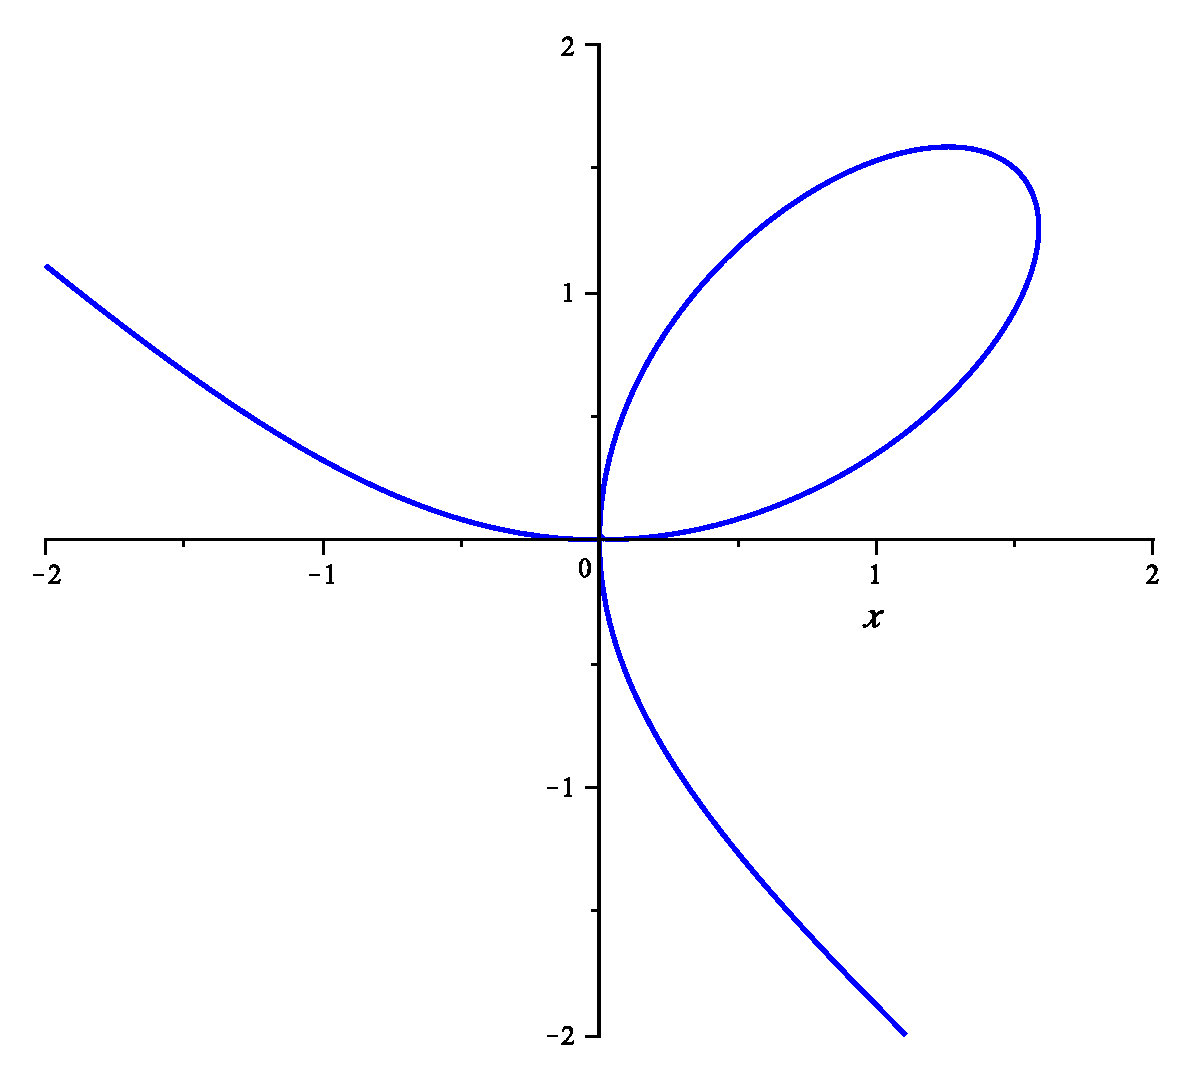
\includegraphics[width=3.1in]{Volumen_2/05_EDO/Figuras/SolImplicita}
\caption{Gr�fica de la funci�n impl�cita $f(x,y) = x^{3} + y^{3}(x) -3xy(x) =0$}
\label{SolImplicita1}
\end{center}
\end{figure}

\subsection{{\color{Fuchsia}Ejemplos}}

\subsection{{\color{red}Practicando con Maxima}}

\subsection{{\color{OliveGreen}Ejercicios}}


\section{Sobre las soluciones}
\subsection{Soluciones expl�citas e impl�citas}
Las soluciones heredan su nombre del tipo  de funci�n que las representa, 
as� tendremos soluci�nes expl�citas cuando las funciones sean soluciones 
y sean expl�citas. Esto es
\[
\frac{\mathrm{d}^{2} y(t) }{ \mathrm{d}t^{2} } = y( t ) +4 \ e^{t} \,\Rightarrow \,
y( t ) =e^{t}C_{2} +e^{-t} C_{1}+ 2 \ t e^{t}
\] 
y tambi�n
\[
y' = (x + y)^{2} \,\Rightarrow \, y( t ) =\tan ( t- C_{1} ) -t \,,\quad \text{con  }  t- C_{1} \neq \frac{\pi}{2}
\]

Las soluciones ser�n impl�citas si son representadas por funciones como
\[
y \ y' + x =0  \,\Rightarrow \, f(x,y)=x^{2} + y( x )^{2} - 25 = 0 \Rightarrow
\left\{
\begin{array}{r l }
  y =    & \sqrt{25 -x^{2}}   \\
  y =    & -\sqrt{25 -x^{2}}  
\end{array}
\quad \text{con } -5 < x < 5
\right.
\] 
En este caso, se tiene que seleccionar una rama de la funci�n ra�z. 

Igualmente, ser� soluci�n impl�cita de la ecuaci�n:
\[
[y^{2}(x) - x]\ y'(x) -y(x) +x^{2} = 0  
\] 
la siguiente funci�n
\[
f(x,y) = x^{3} + y^{3}(x) -3xy(x) =0, 
\] 
ahora no es tan f�cil verificar si efectivamente es una soluci�n. Para comprobarla derivamos la funci�n 
\[
\frac{ \mathrm{d} [ f(x,y)]  }{ \mathrm{d} x } = \frac{ \mathrm{d} \left[ x^{3} + y^{3}(x) -3xy(x) \right] }{ \mathrm{d} x } = 0 \Rightarrow  
3x^{2} +3 y^{2}(x) \frac{ \mathrm{d} y( x) }{ \mathrm{d}x}  - 3y( x ) - 3x \frac{\mathrm{d} y(x) }{\mathrm{d}x } = 0\,,
\]
simplificando y agrupando obtenemos la ecuaci�n diferencial. Otra vez, la funci�n soluci�n no es univaluada. Al graficarla (ver Figura \ref{SolImplicita1}) nos damos cuenta que tenemos varias soluciones de funciones 
univaluadas unas cont�nuas y otras no. La funci�n es univaluada fuera del l�bulo. Esto es para $x \leq 0 \ \wedge \ x > 2^{\frac{2}{3}}$. Con lo cual tendremos que seleccionar, dentro del l�bulo, cu�l de las partes univaluadas corresponde a la soluci�n. 

\subsection{Soluciones generales y particulares}
Veamos las siguientes ecuaciones y soluciones
\[
\begin{array}{r c l}
  y' = e^{x}    & \leftarrow & y(x)= e^{x} + C_{1}   \\
  y'' = e^{x}   & \leftarrow & y(x)= e^{x} + C_{2}x + C_{1}   \\
  y''' = e^{x}  & \leftarrow & y(x)= e^{x}+ C_{3}x^{2} + C_{2}x + C_{1} 
\end{array}
\]
Cada una de las soluciones representan familias de soluciones, una para cada constante. Este tipo de soluciones las denominaremos soluciones generales. Es decir, llamaremos soluci�n general de una ecuaci�n diferencial aquella que queda indeterminada por un conjunto de constantes $\{  C_{1},  C_{2}, C_{3},  \dots , C_{n} \} $.  En contraste, cuando \textit{particularizamos} los valores de las constantes tendremos una soluci�n \textit{particular} par cada una de las ecuaciones. Adicionalmente, cuando nos referimos a las ecuaciones no lineales el concepto de soluci�n particular var�a. Soluciones particulares en este tipo de ecuaciones ser�n aquellas que se cumplen para rangos (o puntos) muy particulares. Vale decir
\[
\left.
\begin{array}{ l }
 (y')^{2} + y^{2} =0     \\
  (y'')^{2} + y^{2} =0         
\end{array}
\right\} \quad \Rightarrow  \quad  y = 0 \quad \text{�nica soluci�n}
\]
Tamibi�n en este caso llamaremos a este tipo de soluciones, particulares. De igual modo puede darse casos para los cuales no exista soluci�n en un determinado intervalo.
\[
\left.
\begin{array}{ l }
 |y'|^{2} + 1 =0     \\
 | y''|^{2} + 1 =0         
\end{array}
\right\}  \quad \Rightarrow  \quad \text{no tienen soluci�n}
\]
Ecuaciones de la forma
\[
x y' =1 \, \Rightarrow\, y(x) = \ln |x| + C \Rightarrow
\left\{
\begin{array}{ l }
   y(x) = \ln ( x )+ C_{1} \text{ para } x > 0   \\
   \\
   y(x) = \ln ( -x )+ C_{1} \text{ para } x < 0      
\end{array} 
\right.
\]
con: $-1 < x< 0\,\wedge \,0< x < 1$, tienen soluciones particulares para intervalos 
de la variables $x$. 

Del mismo modo 
\[
(y' -y ) ( y' - 2y ) = 0 \quad \Rightarrow  \left[ y(x) - C_{1} e^{x} \right] \left[ y(x) - C_{2} e^{2x}\right] = 0
\]
tendr� dos soluciones particulares. 

\subsection{Familia de soluciones $n-$param�tricas}
Si $y(x)= f(x,C_{1},C_{2},\dots ,C_{n}) $ es soluci�n de una ecuaci�n diferencial 
\[ \mathcal{F}[ x,y(x),y'(x),y''(x),\cdots,y^{(n)}(x)] = 0 \,,
\]
para $n$ constantes  $ \{  C_{1}, C_{2}, C_{3}, \dots ,C_{n} \}$  arbitrarias, entonces diremos que 
 \[
 y(x)= f(x,C_{1},C_{2},\dots ,C_{n}) \quad \text{es una familia } n\text{-param�trica de soluciones.}
 \]
Existe una diferencia entre una soluci�n general de una ecuaci�n y una soluci�n $n-$param�trica. La soluci�n general tiene que contener \textbf{todas} las soluciones de una ecuaci�n diferencial determinada. Una soluci�n $n-$param�trica no necesariamente. Veamos
\[
y = xy' +(y')^{2} \quad \Rightarrow \quad
\left\{
\begin{array}{ l }
   y(x) = C x + C^{2}   \\
   \\
   y(x) = -\dfrac{x^{2}}{4}      
\end{array} 
\right.
\] 
Se estar�a tentado en llamar soluci�n general a la soluci�n $1-$param�trica $y = C x + C^{2}$. Sin embargo, se deja por fuera a la otra soluci�n que no tiene que ver con un valor particular de la constante $C$. 

Otro ejemplo, lo constituye
\[
y' = -2 y^{\frac{3}{2}} \quad \Rightarrow \quad  y(x) = \frac{{C}^{2}}{ \left( Cx+1 \right)^{2}} \,,
\,\,\, \forall \, x \,,
\]
pero tambi�n
\[
y(x) =  \left( x+ \tilde{C} \right)^{-2}  \,, \,\, \text{es soluci�n con }  \, y(x) \neq 0\,.
\]

Una soluci�n $n-$param�trica se denominar� soluci�n general si contiene \textbf{todas} las soluciones de una determinada ecuaci�n diferencial. En el caso de ecuaciones diferenciales lineales, las soluciones $n-$param�tricas constituyen las soluciones generales a las ecuaciones diferenciales.

\subsection{Soluci�n particular,  valores iniciales y valores de contorno}
Dependiendo de la situaci�n f�sica que estemos modelando quiz� podamos determinar las constantes arbitrarias de una familia $n-$param�trica con informaci�n para un �nico punto $x = x_{0}$. Esto es:
\[
\mathcal{F}[ x,y(x),y'(x),y''(x),\cdots,y^{(n)}(x)] = 0 \quad \Rightarrow \quad  y(x)= f(x,C_{1},C_{2},\dots C_{n})  
\]
donde
\[
y(x_{0}) = C_{1}  \quad y'(x_{0}) = C_{2}  \quad \dots \quad   y^{(n-1)}(x_{0}) = C_{n}\,.
\]
En este caso diremos que tendremos un problema de valores iniciales, ya que determinamos las constantes arbitrarias a partir de la informaci�n de la funci�n y sus derivadas en un solo punto, por ejemplo:
\[
y'' + \omega^{2} y = 0 \quad \text{con } 
\left\{
\begin{array}{ l }
   y(0) = 0       \\
   y'(0) = 1         
\end{array}
\right\} \quad \Rightarrow \quad
y(x) = \frac{1}{\omega} \mathrm{sen}( \omega x)\,.
\]
Si por el contrario, para determinar el valor de las constantes arbitrarias disponemos de informaci�n de la funci�n y sus derivadas en dos o m�s puntos, diremos que tendremos un problema de contorno. Esto es:
\[
y'' + \omega^{2} y = 0 \quad \text{con } 
\left\{
\begin{array}{ l }
   y(0) = 0       \\
   y(1) = 0         
\end{array}
\right\} \quad \Rightarrow \quad
y(x) =  \mathrm{sen}( n \pi \omega x)\,.
\]
N�tese que tambi�n pudimos haber tenido informaci�n del tipo 
\[
y(0) =  y_{0}\,,\, y'(1) = y_{1}\,;\, y'(0) =  y_{0}\,,\, y'(1) = y_{1}\,;\, 
y'(0) =  y_{0}\,,\, y(1) = y_{1}\,,
\]
y para cada uno de estos caso tendremos una soluci�n distinta. 

Demostraremos que los problemas de valores iniciales para ecuaciones diferenciales lineales siempre tienen soluci�n particular (siempre se pueden determinar las constantes a partir de la informaci�n de la funci�n y las derivadas en UN punto). No as� los problemas de valores de contorno.

\subsection{{\color{Fuchsia}Ejemplos}}

\subsection{{\color{red}Practicando con Maxima}}

\subsection{{\color{OliveGreen}Ejercicios}}

%\newpage

\chapter{Ecuaciones diferenciales de orden 1}
\label{CapEDO1}
\section{Soluciones anal�ticas}

Es fundamental, primero que todo, identificar con que tipo de ecuaci�n diferencial ordinaria que 
estamos tratando antes de cualquier intento de conseguir una soluci�n. 
Veamos varios ejemplos:
\[
\begin{array}{r l l l }
\dfrac{\mathrm{d}^2 \theta}{\mathrm{d}t^2}+\dfrac{g}{l}\mbox{sen}(\theta) &=&0\,, & \text{ EDO no lineal, homog�nea de orden }2  \\   &   \\
\dfrac{\mathrm{d}^2 \theta}{\mathrm{d}t^2}+\dfrac{g}{l} \theta &=&0\,, & \text{ EDO  lineal, homog�nea de orden }2  \\   &   \\ 
\dfrac{\mathrm{d}^2 \theta}{\mathrm{d}t^2}+\dfrac{g}{l} \theta &=&E(t)\,, & \text{ EDO lineal, no homog�nea de orden }2  \\   &   \\
y^{\prime}+xy  &=&\dfrac{x}{y^3}\,, & \text{ EDO no lineal, homog�nea de orden }1  \\   &   \\
y^{\prime}-x^3+2\frac{y}{x} -\frac{1}{x}y^2 &=&0\,, & \text{ EDO no lineal, no homog�nea de orden }1  \\   &   \\
\tan(x) y^{\prime}-y &=&\tan^2(x)\,, & \text{ EDO  lineal, homog�nea de orden }1  \\   &   \\
xy^{\prime}+y &=&x^3\,, & \text{ EDO lineal, no homog�nea de orden }1  \\   &   \\ 
\end{array}
\]

Ahora de manera un poco m�s sistem�tica diremos que una ecuaci�n diferencial de primer orden ser� un funcional tal que si es expl�cita respecto a la derivada �sta se podr� despejar
\[
\mathcal{F}[x,y(x),y'(x)]=0 \quad \Rightarrow \quad
\left\{
\begin{array}{ l}
 y' \equiv  \dfrac{ \mathrm{d} y(x)}{\mathrm{d}x}  = H(x,y)         \\
          \\
  P(x,y)\mathrm{d}x +  Q(x,y)\mathrm{d} y = 0    
\end{array}
\right.
\]
\paragraph{Ejemplos:}
\begin{eqnarray*}
y^{\prime}=2xy+e^x  \,&\Rightarrow&\, \left(2xy-e^x \right)\mathrm{d}x-\mathrm{d}y=0 \,,\\ \\
y^{\prime}=\ln(x)+y \,&\Rightarrow&\, \left(\ln(x)+y \right)\mathrm{d}x-\mathrm{d}y=0
\end{eqnarray*}

\subsection{M�todos elementales de integraci�n}
Para comenzar expondremos unos m�todos de integraci�n, los cuales si bien son elementales y casi triviales ser�n utilizados en lo que sigue con bastante frecuencia.

\subsubsection{Integraci�n directa}
La integraci�n directa tiene varias variantes las cuales nos hemos tropezado en varias situaciones de modelaje y que nos han permitido integrar (intuitivamente) ecuaciones diferenciales. La m�s directa de todas tiene que ver con la siguiente ecuaci�n diferencial
\[
\frac { \mathrm{d} y( x) }{ \mathrm{d}x} = f(x) 
\]
por lo cual, al integrar (anal�tica o num�ricamente) tendremos la expresi�n para  la funci�n $ y( x)$,
\[
\int  \mathrm{d} y( x) = \int  \mathrm{d}x \ f(x)  \quad \Rightarrow \quad y( x) =  \int  \mathrm{d}x \ f(x) +C
\]

La integraci�n directa fue la estrategia que utilizamos anteriormente para encontrar las formulitas que nos aprendimos en bachillerato. Esto es
\[
 \frac{\sum F_{ext}}{m} = \frac{\mathrm{d}v(t)}{\mathrm{d}t} = a = \text{constante} \quad \Rightarrow \quad
\left\{
\begin{array}[l]{l}
v(t)=\int\mathrm{d}t\ a=  a t+C_{1}\\
\\
x(t)=\int\mathrm{d}t\ \left(at+C_{1}\right)  = a\dfrac{t^{2}}{2} +C_{1}t+C_{2}
\end{array}
\right.
\] 
en la cual al recordar las condiciones iniciales  se tiene:
\[
\begin{array}{lll }
   v(0) = v_{0} \equiv C_{1}   & \Rightarrow &v(t) =v_{0} +at \\ 
      &  &  \\
  x(0) = x_{0} \equiv C_{2}    & \Rightarrow & x(t) = x_{0} + v_{0}t + a \dfrac{t^{2}}{2}\,.
 \end{array}
\]

Una primera variante de la estrategia de integraci�n directa anterior se aplica a la siguiente ecuaci�n
\[
\frac { \mathrm{d} y( x) }{ \mathrm{d}x} = f(y)  
\]
acomodando los t�rminos e integrando resulta:
\[
\int  \frac { \mathrm{d} y }{f(y)  } = \int  \mathrm{d}x  \quad \Rightarrow \quad \mathcal{F}[ y( x) ] = x + C
\]
donde $  \mathcal{F}[ y( x) ] $ ser� un funcional, desde el cual quiz� se pueda despejar $y( x)$. 

Esta estrategia se ilustra en el siguiente ejemplo:
\[
\frac { \mathrm{d} y( x) }{ \mathrm{d}x}  =-ay \left( x \right)\,, \text{ con } y(0) =2\,,
\] 
entonces:
\[
\int \frac{ \mathrm{d} y }{y} = -a \int \mathrm{d}x \quad\Rightarrow \quad  y(x) = C e^{-ax} 
\quad\Rightarrow \quad y_{p}(x) = 2 e^{-ax}\,.
\]
la Figura \ref{fam1param} muestra varias soluciones particulares pertenecientes a esta familia, 
para $a = \frac{1}{3}$. 

\begin{figure}
\begin{center}
\includegraphics[width=3.6in]{Volumen_2/06_EDO_1/Figuras/fam1para}
\caption{Familia de soluciones $1-$param�trica para $a = \frac{1}{3}$. En particular han sido tomados los valores $C = -3,-2,-1, 0, 1,2,3$ }
\label{fam1param}
\end{center}
\end{figure}

Otro ejemplo de integraci�n directa se puede ver en la b�squeda de la soluci�n de la siguiente ecuaci�n
diferencial no lineal:
\[
yy' = (y + 1)^{2}  
\]
esto es:
\[
\frac{yy'}{ (y + 1)^{2}} = 1 \quad \Rightarrow \quad
\int \frac{y \mathrm{d} y}{(y + 1)^{2}} = \int \mathrm{d}x\,, \text{ para } y \neq -1 \,,
\]
integrando
\[
\frac{1}{y +1} + \ln |y + 1 | = x + C \,,
\]
que no es otra cosa que una familia de soluciones impl�citas, $1-$param�trica. 
Para una condici�n inicial como $y(2) = 0$ entonces 
\[
y(2) = 0  \Rightarrow C = -1 \quad  \Rightarrow \frac{1}{y +1} + \ln |y + 1 | = x -1  \text{ para } y \neq -1 \,,
\]
una vez m�s esta familia de soluciones $1-$param�trica no constituye la soluci�n general de la
ecuaci�n diferencial ya que no contiene todas las soluciones. En este caso, $y(x)=-1$ tambi�n es soluci�n.

\subsection{Ecuaciones diferenciales separables}
Los casos anteriores de integraci�n directa son generalizados por una ecuaci�n que llamaremos separable.  Esto es, la funci�n (funcional) de dos variables del lado derecho se supone que es el resultado del  producto de dos funciones de una variable, con lo cual las variables dependientes e independientes se agrupan a lados distintos de la igualdad. La siguiente ecuaci�n es separable
\[
\frac { \mathrm{d} y( x) }{ \mathrm{d}x}  = F[y(x)]G(x)   
\]
y por lo tanto
\[
\frac { \mathrm{d} y(x) }{ F(y) }  = G(x) \ \mathrm{d}x  \quad \Leftrightarrow \quad
\int \frac { \mathrm{d} y }{ F(y) }  = \int G(x) \ \mathrm{d}x\,.
\]
Por ejemplo, al querer resolver la siguiente ecuaci�n
\[
\frac { \mathrm{d} y( x) }{ \mathrm{d}x}  = x + xy  
\] 
se tiene
\[
\int \dfrac{\mathrm{d} y}{ 1 + y} = \int x \ \mathrm{d}x \quad  \Rightarrow \quad
\ln (1 +y) = \frac{x^{2}}{2} +C \quad  \Rightarrow \quad y(x) = A e^{\frac{x^{2}}{2}} -1 \,,
\] 
donde $C$ o $A$ son constantes arbitrarias a ser determinadas por las condiciones iniciales 
y adem�s con $y  \neq -1$. De todos modos $y=-1$ es una soluci�n particular.

\subsection{Variaciones sobre separabilidad}
Existen otras situaciones en las cuales encontremos ecuaciones diferenciales que podremos convertir en separables a trav�s de un cambio de variable:
\[
\frac { \mathrm{d} y}{ \mathrm{d}x}  = f(\underbrace{ax + by + c}_{z}) \quad \Rightarrow \quad
\mathrm{d}z = a\,\mathrm{d}x + b\, \mathrm{d}y  \,,
\]
por lo tanto:
\[
\dfrac{\mathrm{d} y}{\mathrm{d} x} = \dfrac{1}{b} \dfrac{\mathrm{d}z}{\mathrm{d}x} -\dfrac{a}{b}
\quad\Rightarrow \quad \dfrac{1}{b} \dfrac{\mathrm{d}z}{\mathrm{d}x} -\dfrac{a}{b} = f(z) \quad\Rightarrow \quad
\dfrac{\mathrm{d}z}{\mathrm{d}x} =  bf(z) + a
\]
es decir, el cambio de variable nos conduce a una ecuaci�n diferencial separable:
\[
\frac{\mathrm{d}z}{bf(z)+a}=\mathrm{d}x\,.
\]

Un ejemplo nos clarifica de qu� se trata
\[
y' = \mathrm{sen}^{2} (x -y)\quad \Rightarrow \mathrm{d}z = \mathrm{d}x -\mathrm{d}y \,,
\]
esto es
\[
y' = 1 - \dfrac{\mathrm{d}z}{\mathrm{d}x} \quad \Rightarrow \quad  z' = 1 -  \mathrm{sen}^{2} (z) 
\quad \Rightarrow \quad \int \dfrac{\mathrm{d}z}{1 -  \mathrm{sen}^{2} (z)} =  \int \mathrm{d}x
\]
es decir
\[
\int \dfrac{\mathrm{d}z}{\cos^{2} (z)} = x + C \, \Rightarrow  \,\tan(z) = x + C \, \Rightarrow \,
 \tan (x - y) = x + C  \, \Rightarrow \, y = x - \arctan(x +C)\,.
\]

Se puede tratar de generalizar el caso anterior y considerar ecuaciones diferenciales del tipo  
\[
\dfrac { \mathrm{d} y }{ \mathrm{d}x}  = f \left( \dfrac{ a_{1}x + b_{1}y + c_{1} }{ a_{2}x + b_{2}y + c_{2} } \right) 
\]
Entonces, se distinguen dos casos dependiendo de si las rectas 
$a_{1}x + b_{1}y + c_{1}=0$ y $a_{2}x + b_{2}y + c_{2} = 0$ son paralelas o no. 
\begin{enumerate}
\item  Son paralelas:
\[
\frac{a_{2}}{a_{1}} = \frac{b_{2}}{b_{1}} = \lambda  \quad \Rightarrow \dfrac { \mathrm{d} y }{ \mathrm{d}x}  = f \left( \dfrac{ a_{1}x + b_{1}y + c_{1} }{ \lambda (a_{1}x + b_{1}y) + c_{2} } \right) \equiv \tilde{f}(a_{1}x + b_{1}y) 
\] 
la cual analizamos anteriormente.


\item No son paralelas, entonces se intuye el siguiente cambio de variables
\[
\begin{array}{l c l c l}
u = a_{1}x + b_{1}y + c_{1} &\Rightarrow & \mathrm{d} u = a_{1}\mathrm{d}x + b_{1}\mathrm{d}y &  &\mathrm{d}x = \dfrac{b_2\mathrm{d} u- b_1\mathrm{d} v}{a_1 b_2 - a_2 b_1}  \\     
&  &  &  \Rightarrow  & \\
v = a_{2}x + b_{2}y + c_{2} &\Rightarrow & \mathrm{d}v = a_{2}\mathrm{d}x + b_{2}\mathrm{d}y &  &\mathrm{d}y = \dfrac{a_1\mathrm{d} v- a_2\mathrm{d} u}{a_1 b_2 - a_2 b_1} 
\end{array}
\] 
con lo cual, la ecuaci�n diferencial
\[
\dfrac { \mathrm{d}y }{ \mathrm{d}x}  = f \left( \dfrac{ a_{1}x + b_{1}y + c_{1} }{ a_{2}x + b_{2}y + c_{2} } \right)=f\left(\frac{u}{v}\right)\,,
\] 
queda de la forma
\[
\left[a_2+ b_2 f\left(\frac{u}{v}\right)\right] \mathrm{d}u -
\left[a_1+ b_1 f\left(\frac{u}{v}\right)\right] \mathrm{d}v  = 0\,,
\]
donde la funci�n $ f \left( \frac{u}{v} \right)$ se conoce como una funci�n homog�nea  al igual que la ecuaci�n diferencial que hereda de �sta su nombre. Este tipo de ecuaciones diferenciales ser�n consideradas en la pr�xima secci�n.  
\end{enumerate}

Otro enfoque (equivalente) de este mismo problema puede ser consultado en el problemario de Kiseliov, Kransnov, Makarenko\footnote{A. Kiseliov, M. Krasnov y G. Makarenko (1969) \textbf{Problemas de Ecuaciones Diferenciales Ordinarias.} (\textit{Mir}, Mosc�)}. En este enfoque el cambio de variables se relaciona con el punto de corte $(x_{0},y_{0})$ 

Para ejemplificar este caso analizaremos un ejemplo sencillo de una funci�n con argumento inhomog�neo del tipo. 
\[
\dfrac { \mathrm{d} y( x) }{ \mathrm{d}x}  = \dfrac{ a_{1}x + b_{1}y + c_{1} }{ a_{2}x + b_{2}y + c_{2} } \quad \Leftrightarrow \quad Q(x,y) \mathrm{d} y + P(x,y)  \mathrm{d}x =0 \quad
\Rightarrow
\left\{
\begin{array}{l}
  Q(x,y) \propto  a_{2}x + b_{2}y + c_{2}      \\
         \\
  P(x,y)    \propto   a_{1}x + b_{1}y + c_{1}
\end{array}
\right.
\] Decimos, entonces que los coeficientes $Q(x,y)$  y  $P(x,y)$ son inhomog�neos ($c_{i}\neq 0$). Supondremos que las rectas no son paralelas, por lo cual utilizamos el cambio de variable propuesto anteriormente. Entonces
\[
\begin{array}{l c l c l}
  u = a_{2}x + b_{2}y + c_{2} &\Rightarrow &   \mathrm{d} u = a_{2}\mathrm{d}x + b_{2}\mathrm{d}y & \Rightarrow \mathrm{d}y = \dfrac{1}{b_{2} - b_{1}} \left( \dfrac{ \mathrm{d} u}{a_{2}} - \dfrac{ \mathrm{d} v}{a_{1}} \right)  \\
     &  &  &  \\
   v = a_{1}x + b_{1}y + c_{1} &\Rightarrow & \mathrm{d}v = a_{1}\mathrm{d}x + b_{1}\mathrm{d}y & \Rightarrow \mathrm{d}x = \dfrac{1}{a_{2} - a_{1}} \left( \dfrac{ \mathrm{d} u}{b_{2}} - \dfrac{ \mathrm{d} v}{b_{1}} \right) 
\end{array}
\] 
con lo cual convertimos los coeficientes $Q(x,y)$  y  $P(x,y)$ en homog�neos. Esto es 
\[
\begin{array}{c }
\underbrace{(a_{2}x + b_{2}y + c_{2}) \mathrm{d} y + (a_{1}x + b_{1}y + c_{1})  \mathrm{d}x =0}          \\
   \Downarrow      \\
\overbrace{\left( \dfrac{u}{a_{2}(b_{2} - b_{1}) } + \dfrac{v}{b_{2}(a_{2} - a_{1})} \right)\mathrm{d}u 
-
\left( \dfrac{u}{a_{1}(b_{2} - b_{1})} + \dfrac{v}{b_{1}(a_{2} - a_{1})} \right) \mathrm{d} v =0  }       
\end{array}
\]
es decir
\[ 
P(u,v) =  u\left( \dfrac{1}{a_{2}(b_{2} - b_{1}) } + \dfrac{\frac{v}{u}}{b_{2}(a_{2} - a_{1})} \right) = u g_{1} \left( \frac{v}{u} \right)\,,
\]
y
\[
 Q(u,v)  = u\left( \dfrac{1}{a_{1}(b_{2} - b_{1})} + \dfrac{\frac{v}{u}}{b_{1}(a_{2} - a_{1})} \right) = u g_{2} \left( \frac{v}{u} \right)\,.
\]

Este tipo de funciones homog�neas ser�n consideradas m�s adelante.

\subsection{Ecuaciones diferenciales no separables}
Veamos ahora un caso bastante sencillo de resolver donde la EDO no es una ecuaci�n 
diferencial separable. Consideremos, a manera de prueba, la ecuaci�n diferencial siguiente
\[
\frac{ \mathrm{d} y( x )}{ \mathrm{d}x} +ay( x) = e^{-x}\,, \text{ con } y(0) =2 \,,
\]
entonces, podemos preguntarnos sobre la posibilidad de que exista una funci�n $\mu(x)$ 
de manera  que si multiplicamos  ambos
lados de la ecuaci�n diferencial por $\mu(x)$ entonces, el lado izquierdo de la ecuaci�n
diferencial se pueda escribir como:
\[
\mu(x) \left[ \frac{ \mathrm{d} y( x )}{ \mathrm{d}x} +ay( x) \right]
\stackrel{?}{\equiv}  \frac{ \mathrm{d} }{ \mathrm{d}x} [ \mu(x) y( x ) ] \,.
\]
De esta manera, la funci�n $\mu(x)$  es una funci�n a determinar (en este caso a adivinar).
Efectivamente tenemos que si
\[
\mu(x) = e^{ax} \,,
\]
entonces al multiplicar ambos lados de la ecuaci�n diferencial por $\mu(x)$, resulta:
\begin{eqnarray*}
e^{ax} \frac{ \mathrm{d} y( x )}{ \mathrm{d}x} + e^{ax}  ay( x)&=& e^{ax} e^{-x}\\
 \frac{ \mathrm{d}}{ \mathrm{d}x}\left[e^{ax} y( x )\right]  &=& e^{(a-1)x} \\
 \int  \mathrm{d} \left[e^{ax} y( x )\right] &=& \int  \mathrm{d}x \ e^{(a-1)x}
\end{eqnarray*}
de forma y manera que: 
\[
e^{ax} y( x ) = \frac{1}{a-1} e^{(a-1)x} + C \,.
\]
Para $y(0) = 2$:
\[
 y( 0 ) = 2= \frac{1}{a-1}  + C \, \,\Rightarrow\, C=\frac{2a -3}{a - 1}
\]
Una soluci�n particular ser� entonces:
\[
 y_{p}(x) = \frac{1}{a -1} \left[ e^{-x} + (2a -3) e^{-ax} \right]\,.
\]

Un par comentarios son pertinentes:
\begin{itemize}
  \item Llamaremos al t�rmino $\mu(x)$ factor integrador de la ecuaci�n diferencial. Este factor 
est� relacionado con propiedades de simetr�a de la ecuaci�n, pero en este nivel lo buscaremos tanteando.
  \item La soluci�n general de esa ecuaci�n diferencial toma la forma de $y(x) =  e^{-x} + C e^{-ax}$, donde el segundo de los t�rminos $y_{H}(x) =C e^{-ax}$ corresponde a la soluci�n general para la ecuaci�n homog�nea asociada a esa ecuaci�n diferencial: $ \frac{ \mathrm{d} y( x )}{ \mathrm{d}x} +ay( x) =0$. El otro t�rmino $ y_{I}(x) = e^{-x}$ corresponde a la soluci�n particular de la inhomog�nea: $\frac{ \mathrm{d} y( x )}{ \mathrm{d}x} +ay( x) = e^{-x}$. 
\end{itemize}
Esto �ltimo ser�
 una propiedad general para ecuaciones diferenciales lineales de cualquier orden. Resolveremos la ecuaci�n homog�nea y luego encontraremos una soluci�n de la inhomog�nea. La soluci�n general ser� una suma de ambas soluciones.
 
En general, para la ecuaci�n  
\[
y' + ay = g(x)\,, \quad \mbox{el factor integrador es:} \,\, \mu(x) = e^{ax} 
\]  
y se tiene la siguiente soluci�n general
\[
y(x) =  \underbrace{e^{-ax} \int_{x_{0}}^{x}  \mathrm{d}t \ g(t) e^{at}}_{\text{soluci�n de la inhomog�nea}}
\quad  + \underbrace{Ce^{-ax}}_{\text{soluci�n de la homog�nea}}
\]  
la demostraci�n la dejamos como ejercicio para el lector.

La figura \ref{EcDifRoad} muestra el mapa de ruta para la resoluci�n de las EDO lineales. 
\begin{figure}[t]
\begin{center}
\includegraphics[width=4.5in]{Volumen_2/06_EDO_1/Figuras/EcDifRoad.png}
\caption{Mapa de las ecuaciones diferenciales expl�citas}
\label{EcDifRoad}
\end{center}
\end{figure}

\subsection{M�todo de las isoclinas}
Este m�todo se basa en la idea de campo y curvas integrales que vimos cuando estudiamos campos vectoriales. La idea es bien simple, en general, una ecuaci�n diferencial de primer orden (expl�cita respecto a la derivada) se podr� representar como:
\begin{equation}
y' = f(y,x) \,.
\end{equation}

Ahora bien, el lado derecho de esa igualdad lo representa una funci�n de dos variables, la cual tendr� un valor en cada punto $(x,y)$. Ese valor (por la igualdad que representa la ecuaci�n diferencial) ser� el valor de la derivada en ese punto y el valor de la derivada en un punto, no es otra cosa que la pendiente de la recta tangente a una curva en ese punto. Con eso, al construir una gr�fica recordamos las curvas integrales de los campos vectoriales y reconstruimos las curvas soluci�n a partir de sus tangentes.

Tenemos entonces que si $y=f(x)$ o $f(x,y)=0$ define $y$ como una funci�n de $x$ que satisface
$y^{\prime} = f(y,x)$ sobre un intervalo $a<x<b$, entonces el gr�fico de esta funci�n se 
denomina una curva integral y a la totalidad de esas curvas se le llama un campo de direcciones.
\begin{figure}[t]
\begin{center}
\includegraphics[width=2.7in]{Volumen_2/06_EDO_1/Figuras/EjemI} (a)
\includegraphics[width=2.6in]{Volumen_2/06_EDO_1/Figuras/EjemII} (b)
\caption{ Isoclinas para los ejemplos (a) y (b)}
\label{FigCampos1}
\end{center}
\end{figure}
\begin{figure}
\begin{center}
\includegraphics[width=2.6in]{Volumen_2/06_EDO_1/Figuras/EjemIII} (c)
\includegraphics[width=2.8in]{Volumen_2/06_EDO_1/Figuras/EjemIV}  (d)
\caption{ Isoclinas para los ejemplos (c) y (d)}
\label{FigCampos2}
\end{center}
\end{figure}
A las curvas con la propiedad: $y^{\prime} = f(x,y)=$ constante se le denominan isoclinas (igual pendiente). 

Por ejemplo, si consideramos la EDO:
\[
y^{\prime} = \frac{y}{x} \, \, \Rightarrow \,\,\, y=Cx \,\leftarrow \mbox{curva integral. }
\quad (x\neq0\,,y\neq0)\,.
\]

O para la ecuaci�n
\[
y^{\prime} = -\frac{x}{y} \, \, \Rightarrow \,\,\, x^2+y^2=C^2 \, \leftarrow \mbox{curva integral. }
\quad (x\neq0\,,y\neq0)\,.
\]

Cuando por un punto pasa m�s de una curva integral lo llamaremos un punto singular y para los puntos por donde pase una y solo una curva integral le llamaremos puntos ordinarios.

La Figura \ref{FigCampos1} contiene la representaci�n gr�fica para las tangentes de las siguientes ecuaciones diferenciales:
\[ 
 \text{(a)} \quad y' = e^{-x} -\frac{1}{3} y  \quad  \qquad \qquad 
 \text{(b)} \quad y' = \frac{y}{x} 
\]
y la Figura \ref{FigCampos2} las de
\[
\text{(c)} \quad y'  = -\frac{x}{y}  \quad  \qquad \qquad \quad
\text{(d)} \quad y'  = 1 +  x y  
\]

En el Cuadrante (a) de la Figura \ref{FigCampos1} se muestran  las soluciones particulares para las condiciones iniciales: $y(0)=0.75, \ 0.50, \ 0,\  -0.50,\ -0.75$. El Cuadrante (b) de la misma figura corresponde a las tangentes generadas a partir de la ecuaci�n diferencial. N�tese que son curvas integrales radiales y que para el punto $x=0$ no est� definida la curva integral. En el Cuadrante (c), de la Figura \ref{FigCampos2},  se representan las tangentes de la ecuaci�n. Finalmente el Cuadrante (d) contiene las tangentes a la ecuaci�n diferencial, en ella se han indicado las curvas integrales para las soluciones particulares correspondientes a las condiciones iniciales: $y(0)=0.75, \ 0.50, \ 0,\  -0.50,\ -0.75$.

Es importante se�alar que este m�todo permite obtener las posibles soluciones de una ecuaci�n diferencial no importa lo complicada que se

\subsection{Ecuaciones diferenciales homog�neas}
Primero que todo, definamos qu� son las funciones homog�neas de grado $n$. 

\begin{mdframed}[linecolor=OliveGreen,linewidth=0.3mm]
\textbf{Definici�n}: Diremos que una funci�n $f(x,y)$ es homog�nea de grado $n$ si 
\[
f(tx,ty)=t^{n}f(x,y) 
\quad \Leftrightarrow \quad 
\left\{
\begin{array}{l}
 \text{si } w=\dfrac{y}{x} \Rightarrow f(x,y) = x^{n}g(w)         \\
          \\
 \text{si } w=\dfrac{x}{y} \Rightarrow f(x,y) = y^{n}h(w)        
\end{array} 
\right.
\]
donde $n$ es una constante y $t>0$.
\end{mdframed}

Las funciones homog�neas indican un comportamiento particular cuando cambiamos la escala de sus variables. Se utilizan con bastante frecuencia en hidrodin�mica y termodin�mica. 

Por ejemplo, la siguiente funci�n: 
\[
f(x,y) = x^{2} + y^{2}\ln \left( \frac{y}{x} \right)\,
\]
es una funci�n homog�nea de grado $2$, ya que: 
\[
f(tx,ty) = (tx)^{2} + (ty)^{2}\ln \left( \frac{ty}{tx} \right) \,\, \Rightarrow \,\,
f(tx,ty) = t^2 \left[ x^{2}  + y^{2}\ln \left( \frac{y}{x} \right)  \right] = t^2 f(x,y)\,.
\]

\begin{mdframed}[linecolor=OliveGreen,linewidth=0.3mm]
\textbf{Definici�n}: Una ecuaci�n diferencial ordinaria de primer orden 
\begin{equation}
P(x,y) \mathrm{d}x + Q(x,y) \mathrm{d}y =0 \label{edo1}\,,
\end{equation}
ser� una ecuaci�n diferencial con coeficientes homog�neos si: 
\[
Q(x,y) \text{ y } P(x,y) \text{ son homog�neas de grado }n \,.
\] 
\end{mdframed}

\begin{mdframed}[linecolor=OliveGreen,linewidth=0.3mm]
\textbf{Teorema}: Si los coeficientes $P(x,y)$ y $Q(x,y)$ de una ecuaci�n diferencial son
homog�neos de orden $n$, entonces la siguiente sustituci�n: $y=ux$, convertir� la ecuaci�n diferencial en una ecuaci�n diferencial donde las variables son separables.
\end{mdframed}

\paragraph{Demostraci�n}
Como $P(x,y)$ y $Q(x,y)$ son funciones homog�neas de orden $n$ (hip�tesis) entonces:
\[
P(x,y)= x^n f(u) \quad \mbox{y} \quad  Q(x,y)= x^n g(u)\,,
\]
sustituyendo en la ecuaci�n diferencial (\ref{edo1}):
\begin{eqnarray*}
x^n f(u) \mathrm{d}x + x^n g(u) (u \mathrm{d}x + x \mathrm{d}u) &=&0 \\
\left[f(u)+ u g(u)\right] \mathrm{d}x + x g(u) \mathrm{d}u &=&0 \\
\left[f(u)+ u g(u)\right] \frac{\mathrm{d}x}{x} +  g(u) \mathrm{d}u &=&0\\
\frac{\mathrm{d}x}{x} + \frac{g(u) \mathrm{d}u}{f(u)+ u g(u)}&=&0\,,
\end{eqnarray*}
donde $x\neq0$ y $f(u)+ u g(u)\neq0$.  $\blacktriangleleft$


El lector, debe demostrar  que la sustituci�n $x=uy$ tambi�n convierte la ecuaci�n diferencial en una de variables separables.

N�tese que exigir que $Q(x,y)$  y  $P(x,y)$  sean funciones homog�neas de grado $n$, equivale a imponer que 
\[
\frac { \mathrm{d} y( x) }{ \mathrm{d}x}  = \dfrac{P(x,y)}{Q(x,y)} \equiv F \left(\frac{y}{x} \right) \quad \text{donde }F \left(\frac{y}{x} \right)  \text{ es homog�na de grado }0\,, 
\] 
con lo cual estamos diciendo que si los coeficientes $Q(x,y)$  y  $P(x,y)$  son
funciones homog�neas de grado $n$, la ecuaci�n diferencial es invariante de escala.

Consideremos  la siguiente ecuaci�n diferencial no linea
\[
x y'  =  { \sqrt{x^{2} - y^{2} } + y }
\]
Esto es
\[
\left( \sqrt{x^{2} - y^{2} } + y \right) \mathrm{d}x - x \mathrm{d}y =0  \,\, \Rightarrow \,\, 
\left\{
\begin{array}{l c l }
 P(tx,ty) = \sqrt{(tx)^{2} -(ty)^{2}}  +ty &   =   & t\left(\sqrt{x^{2}-y^{2}}+y \right)   \\
   &	& \\
  Q(tx,ty) =-   tx   &      &   
\end{array}
\right.
\]
los coeficientes son funciones homog�neas de grado $1$ y por lo tanto al hacer $y = ux$  tendremos
\[
x\left( \sqrt{1 - u^{2} } + u \right) \mathrm{d}x - x( u\mathrm{d}x + x\mathrm{d}u ) = 0  \,\, \Rightarrow \,\,
\pm\sqrt{1 - u^{2} }  \mathrm{d}x - x\mathrm{d}u = 0 \,\,\Rightarrow \,\,\int \dfrac{ \mathrm{d}x}{x} = \pm \int \dfrac{\mathrm{d}u}{\sqrt{1 - u^{2} }}\,.
\] 
Notemos que: $u \neq \pm 1$ y $x\neq 0$.
Integramos y, finalmente, llegamos a 
\[
\begin{array}{r c r l }
 \ln|x| = \mathrm{arcsen}(u) + C     & \Rightarrow &  \ln|x| = \mathrm{arcsen}\left(\dfrac{y}{x} \right) + 
 C\,, & \text{ para } \left| \dfrac{y}{x} \right| <1 \text{ con } x >0 \\
      &    &  &  \\
- \ln|-x| = \mathrm{arcsen}(u) + C     & \Rightarrow & - \ln|-x| = \mathrm{arcsen}\left(\dfrac{y}{x} \right) + 
C\,, & \text{ para } \left| \dfrac{y}{x} \right| <1 \text{ con } x < 0 \,.
\end{array}
\] 
En este caso tenemos que $u =  \left| \dfrac{y}{x} \right| =1 \,\, \Rightarrow \,\, y = \pm x$ tambi�n es soluci�n.


\subsection{Ecuaciones is�baras}
Las ecuaciones is�baras generalizan a las ecuaciones homog�neas por cuanto los coeficientes de la ecuaci�n $Q(x,y)$  y  $P(x,y)$ no son funciones homog�neas del mismo grado y se busca una transformaci�n que convierta la ecuaci�n en homog�nea. Es decir, si la dimensionalidad en potencias de $y$ es la misma que la dimensionalidad en potencias de $x$. Diremos que una ecuaci�n diferencial es is�bara si cumple con
\begin{eqnarray*}
P(x,y)  \mathrm{d}x &+& Q(x,y) \mathrm{d} y  =0 \\
&\Downarrow&\\
 Q(tx,t^{m}y) & \rightarrow    &  t^{n} P(x,y)   \\
 P(tx,t^{m}y) & \rightarrow    &  t^{n-m+1} Q(x,y)
\end{eqnarray*}
y el cambio de variable que se impone es $y = vx^{m}$. Con lo cual habr� que estudiar si es posible ``balancear'' el orden de las dimensionalidades de variables y funciones.

Tratemos con un ejemplo para ilustrar las ecuaciones is�baras. Consideremos la ecuaci�n 
\[
2xy y' +  y^{2} + \frac{2}{x}   =0\,, \quad \text{entonces, } 
\]
\[
 \left( y^{2} + \frac{2}{x} \right) \mathrm{d}x +  2xy \mathrm{d}y = 0
\,\,  \Rightarrow \,\,
 \left\{
\begin{array}{l c l}
  x \rightarrow x   & \leftrightarrow &  \mathrm{d}x = \mathrm{d}x  \\
	  y \rightarrow z^{m}  & \leftrightarrow &  \mathrm{d}y = m z^{m-1} \mathrm{d}z     
\end{array}
\right.
\]

En la contabilidad de los exponentes de $x$ aporta un peso de $1$ mientras que $y$ aporta un peso de $m$. La intenci�n es balancear los t�rminos para que la ecuaci�n sea homog�nea de grado $n$. Esto es
\begin{eqnarray*}
\left( z^{2m} + \frac{2}{x} \right) \mathrm{d}x &+&  2xz^{m}  m z^{m-1} \mathrm{d}z = 0 \\
\left( z^{2m} + \frac{2}{x} \right) \mathrm{d}x &+&  2mxz^{-1}  z^{2m} \mathrm{d}z = 0 
  \, \Rightarrow \, m = -\frac{1}{2} \, \Rightarrow \, y = vx^{m} \,\Rightarrow \, y=\frac{v}{\sqrt{x}}
\end{eqnarray*}
El exponente del primer t�rmino es $2m$, del segundo $-1$ del tercero $2m$. Al balancear todos los exponentes tendremos $2m=-1$, con lo cual $m = -\frac{1}{2}$.
 \[
\left( \frac{v^{2}}{x} + \frac{2}{x} \right) \mathrm{d}x +  2x \frac{v}{\sqrt{x}}
\left( \frac{\mathrm{d}v}{\sqrt{x}} - \frac{1}{2}\frac{v}{x\sqrt{x}}\mathrm{d}x \right)  = 0 
 \, \Rightarrow v \mathrm{d}v + \frac{\mathrm{d}x}{x}=0
 \] 
 entonces al integrar y devolver el cambio $v =y\sqrt{x}$ tendremos
 \[
\int \mathrm{d}v  \ v + \int  \frac{\mathrm{d}x}{x}=0  \, \Rightarrow 
\frac{v^{2}}{2} + \ln |x| = c  \, \Rightarrow \frac{1}{2}y^{2}x + \ln |x| = c\,.
 \]

\subsection{Ecuaciones diferenciales exactas}

El segundo grupo de estrategias apunta a escribir una ecuaci�n diferencial como una derivada total de un conjunto de funciones. Uno se ayuda en una posible funci�n que pueda acomodar los t�rminos de la ecuaci�n. Esa funci�n se denomina factor integrador, para una ecuaci�n diferencial lineal de primer orden
\[
\frac{ \mathrm{d} y(x)}{ \mathrm{d}x}+f(x) y(x)=g(x)\,,
\]
al multiplicar a ambos lados por $\mu(x)$ resulta
\[
\mu(x) \frac{ \mathrm{d}  y( x ) }{ \mathrm{d}x} + \mu(x) f(x) y(x) =  \mu(x) g(x)\,,
\]
por otro lado, tenemos y queremos que
\[
\frac{ \mathrm{d}} { \mathrm{d}x}  [ \mu(x) y( x ) ] \equiv \mu(x) \frac{ \mathrm{d} y( x ) }{ \mathrm{d}x}+ \frac{ \mathrm{d} \mu(x)}{ \mathrm{d}x} y(x) =  \mu(x) g(x) \,,
 \]
para que esas dos �ltimas ecuaciones sean equivalentes los coeficientes de $y(x)$ tienen que ser iguales, es decir, 
\[
\frac{ \mathrm{d} \mu(x)}{ \mathrm{d}x} = \mu(x) f(x) \,\,\Rightarrow \,\,
\int \frac{ \mathrm{d} \mu(x)}{ \mu(x)} =  \int \mathrm{d}x \ f(x)  \,\, \Rightarrow \,\,
\mu(x) = e^{ \int \mathrm{d}x \ f(x)}
\]
Con lo cual hemos demostrado que para una ecuaci�n lineal de primer orden, siempre es posible encontrar un factor integrador $\mu(x)$ tal que la ecuaci�n diferencial pueda ser expresada como una derivada total del factor integrador y la funci�n inc�gnita.
\[
\frac{ \mathrm{d}  y( x ) }{ \mathrm{d}x} +  f(x) y(x) =   g(x) \,\, \Rightarrow \,\,
\frac{ \mathrm{d}} { \mathrm{d}x} [ \mu(x) y( x ) ] =  \mu(x) g(x) \,\,\Rightarrow \,\,
y(x) = \dfrac{1}{\mu(x)} \left[\int \mathrm{d}x \,  \mu(x) g(x) + C \right]
\]
donde $ \mu(x) = e^{ \int \mathrm{d}x \ f(x)}$\,.

\begin{mdframed}[linecolor=OliveGreen,linewidth=0.3mm]
\textbf{Definici�n}: Una ecuaci�n diferencial de la forma
\[
P(x,y)\mathrm{d}x + Q(x,y)\mathrm{d}y =0 \,,
\]
se llama una ecuaci�n diferencial exacta si esta es el diferencial total de 
alguna funci�n $f(x,y)$, es decir, si:
\[
P(x,y) =\frac{\partial}{\partial x} f(x,y) \quad \mbox{ y } \quad
Q(x,y) =\frac{\partial}{\partial y} f(x,y)\,.
\]
\end{mdframed}

\begin{mdframed}[linecolor=OliveGreen,linewidth=0.3mm]
\textbf{Teorema}: Una condici�n necesaria y suficiente para que la ecuaci�n diferencial 
\[
P(x,y)\mathrm{d}x + Q(x,y)\mathrm{d}y =0 \,,
\]
sea exacta es que:
\[
\frac{\partial}{\partial y} P(x,y) = \frac{\partial}{\partial x} Q(x,y)\,,
\]
donde las funciones: $P(x,y)$, $Q(x,y)$, $\partial_y P(x,y)$, $\partial_x Q(x,y)$ deben existir y ser cont�nuas.
\end{mdframed}

\paragraph{Demostraci�n} Vamos a probar que si: $P(x,y)\mathrm{d}x + Q(x,y)\mathrm{d}y =0$, entonces:
$\partial_y P(x,y) =\partial_x Q(x,y)$.

Como la ecuaci�n es exacta, por la definici�n anterior se tiene que:
\[
P(x,y) = \frac{\partial}{\partial x} f(x,y) \quad \wedge \quad 
Q(x,y) =\frac{\partial}{\partial y} f(x,y)\,,
\]
y como suponemos que $P(x,y)$, $Q(x,y)$, $\partial_y P(x,y)$, $\partial_x Q(x,y)$ existen y 
son cont�nuas:
\[
\frac{\partial}{\partial y} \frac{\partial}{\partial x} f(x,y) \quad \wedge \quad
\frac{\partial}{\partial x} \frac{\partial}{\partial y} f(x,y) \quad \exists\,,
\]
y como:
\[
\frac{\partial}{\partial y} \frac{\partial}{\partial x} f(x,y) =
\frac{\partial}{\partial x} \frac{\partial}{\partial y} f(x,y) \,,
\]
por lo tanto tenemos que una condici�n necesaria es:
\[
\frac{\partial}{\partial y} P(x,y)= \frac{\partial}{\partial x}Q(x,y)\,.
\]

Por otro lado, probemos que si: $\partial_y P(x,y)=\partial_x Q(x,y)$ entonces: 
$P(x,y)\mathrm{d}x + Q(x,y)\mathrm{d}y =0$ es exacta.

As�, para una ecuaci�n diferencial que pueda ser escrita como
\[
\mathrm{d}\left[f(x,y) \right] =0 \,\,\stackrel{?}{\Leftrightarrow} \,\, P(x,y) \mathrm{d} x + Q(x,y)  \mathrm{d}y =0 
\,\, \Rightarrow \,\,
\mathrm{d}\left[f(x,y) \right]  = \dfrac{\partial f(x,y)}{\partial x } \mathrm{d}x +  \dfrac{\partial f(x,y)}{\partial y }\mathrm{d}y =0
\]
donde $f(x,y) $ ser� la funci�n a determinar. 

Entonces tendremos que la condici�n necesaria y suficiente para que una ecuaci�n diferencial sea exacta es  
\[
\left.
\begin{array}{ c }
P(x,y) \Leftrightarrow \dfrac{\partial f(x,y)}{\partial x }    \\
			\\
Q(x,y) \Leftrightarrow \dfrac{\partial f(x,y)}{\partial y }    \\
\end{array}
\right\}
\,\,\Rightarrow \,\, \dfrac{\partial^{2} f(x,y)}{\partial y \partial x } \equiv 
 \dfrac{\partial^{2} f(x,y)}{\partial x \partial y }
\,\, \Leftrightarrow  \,\, \dfrac{\partial P(x,y)}{ \partial y } \equiv \dfrac{\partial Q(x,y)}{\partial x } 
\,\, \Rightarrow \,\, \mathrm{d}\left[f(x,y) \right] =0
\]

Si esto se cumple entonces, podremos encontrar la funci�n $f(x,y) $ integrando respecto a cualquiera de las variables (ahora consideradas independientes ambas)
\[
P(x,y) \equiv \dfrac{\partial f(x,y)}{\partial x } \Leftrightarrow 
f(x,y) = \int_{x_0}^{x}   P(u,y) \mathrm{d}u + S(y)  \Rightarrow
Q(x,y) = \dfrac{\partial f(x,y)}{\partial y } = \dfrac{\partial }{\partial y }  \int_{x_0}^{x}  P(u,y) \mathrm{d}u +
 \dfrac{\mathrm{d} S(y)}{\mathrm{d} y }
\]
entonces 
\[
Q(x,y) =  \int_{x_0}^{x}  \dfrac{\partial P(u,y)}{\partial y } \mathrm{d}u + 
\dfrac{\mathrm{d} S(y)}{\mathrm{d} y } \equiv 
\int_{x_0}^{x}   \dfrac{\partial Q(v,y)}{\partial v } \mathrm{d}v + \dfrac{\mathrm{d} S(y)}{\mathrm{d} y } =
\left. Q(v,y) \right|_{v=x_{0}}^{v=x} + \dfrac{\mathrm{d} S(y)}{\mathrm{d} y }
\]
con lo cual nos queda finalmente otra ecuaci�n diferencial para encontrar  $S(y)$ y con ella $f(x,y)$. Esto es 
\[
\dfrac{\mathrm{d} S(y)}{\mathrm{d} y } = Q(x_{0},y) \,  \Rightarrow  \, 
S(y) =   \int_{y_0}^{y}  Q(x_{0},w) \mathrm{d} w  \,  \Rightarrow  \, 
f(x,y) = \int_{x_0}^{x} P(u,y) \mathrm{d}u  + \int_{y_0}^{y}  Q(x_{0},w) \mathrm{d}w = C\,. \,\, \blacktriangleleft
\]

Hay que hacer notar que los segmentos de l�nea que unen el punto $(x_{0},y_{0})$ con los puntos gen�ricos $(x,y_{0}) \wedge (x_{0},y)$ pertenecen al entorno de $(x_{0},y_{0})$. Este tipo de entornos tambi�n se denomina \textit{multiplemente conexo}.

Notemos que adem�s de demostrar el teorema tambi�n encontramos una familia $1$-param�trica de soluciones:
\[
f(x,y)=  \int_{x_0}^{x}  P(u,y)\mathrm{d}u  + \int_{y_0}^{y} Q(x_{0},w) \mathrm{d}w = C\,.
\]

Consideremos la siguiente ecuaci�n diferencial no lineal
\[
[x  \mathrm{sen}(y) -y^{2}] y' = {\cos(y)}\,.
\]
Entonces:
\[
y'\left[x  \mathrm{sen}(y) -y^{2} \right]= \cos(y) \,\, \Leftrightarrow \,\,
\cos(y) \, \mathrm{d}x - \left(x  \mathrm{sen}(y) -y^{2} \right) \mathrm{d}y =0 \,\,  \Rightarrow  \,\,
\left\{
\begin{array}{ l c l}
P(x,y) & = & \cos(y)    \\
	& &			\\
Q(x,y) & =& - \left(x  \mathrm{sen}(y) -y^{2} \right)    \\
\end{array}
\right.
 \]
y verificamos que esta ecuaci�n diferencial es exacta, ya que 
 \[
 \dfrac{\partial Q(x,y)}{ \partial x } = \dfrac{\partial P(x,y)}{\partial y } = -\sen(y)  \,\,  \Rightarrow \,\,
 f(x,y) = \int_{x_0}^{x}  P(u,y) \mathrm{d}u + \int_{y_0}^{y}  Q(x,w)\mathrm{d}w  = C 
 \]
 con lo cual, si particularizamos el punto $(x_{0},y_{0}) \equiv (0,0)$ tendremos que
 \[
 f(x,y) = \int_{x_0}^{x}  \cos(y) \mathrm{d}u + \int_{y_0}^{y} w^{2} \mathrm{d}w=C 
  \quad  \Rightarrow
  x \cos(y) + \dfrac{y^{3}}{3} = C
 \]


\subsection{Ecuaciones diferenciales lineales de orden 1}
Una ecuaci�n diferencial lineal de orden 1
\[
\frac{ \mathrm{d} y(x)}{ \mathrm{d}x}+f(x) y(x)=g(x)\,,
\]
no es exacta, ya que:
\[
\left[ f(x)y(x)-g(x) \right]\mathrm{d}x +  \mathrm{d}y =0\quad  \Rightarrow 
\left\{
\begin{array}{ l c l}
P(x,y) & = &f(x)y(x)-g(x)    \\
	& &			\\
Q(x,y) & =& 1    \\
\end{array}
\right.  \,\, \Rightarrow \,\,
 \dfrac{\partial Q}{ \partial x } \neq \dfrac{\partial P}{\partial y } \,.
\]
pero como ya vimos,  si $\mu(x)$ es un factor integrador, entonces:
\[
\mu(x)\left[ f(x)y(x)-g(x) \right]\mathrm{d}x +  \mu(x)\mathrm{d}y =0\quad  \Rightarrow 
\left\{
\begin{array}{ l c l}
P(x,y) & = & \mu(x)\left[ f(x)y(x)-g(x) \right]    \\
	& &			\\
Q(x,y) & =& \mu(x)   \\
\end{array}
\right.
\]
y por lo tanto
\begin{eqnarray*}
\partial_x \mu(x) &=& \partial_y \{ \mu(x)\left[ f(x)y(x)-g(x) \right]\}\\
\dfrac{\mathrm{d} \mu(x)}{\mathrm{d} x } &=& \mu(x) f(x)\\
\dfrac{\mathrm{d} \mu(x)}{\mu(x) } &=&  f(x)\mathrm{d} x \,\Rightarrow \, 
\int \dfrac{\mathrm{d} \mu(x)}{\mu(x) } =  \int f(x)\mathrm{d} x \,\Rightarrow \,
\ln|\mu(x)|=\int f(x)\mathrm{d} x \,,
\end{eqnarray*}
es decir,
\[
\mu(x) = e^{\int f(x)\mathrm{d} x}\,.
\]
Esto significa que para las ecuaciones lineales de orden $1$ se tiene
\[
e^{\int f(x)\mathrm{d} x}\left[ f(x)y(x)-g(x) \right]\mathrm{d}x +  e^{\int f(x)\mathrm{d} x}\mathrm{d}y =0\quad  \Rightarrow 
\left\{
\begin{array}{ l c l}
P(x,y) & = &e^{\int f(x)\mathrm{d} x}\left[ f(x)y(x)-g(x) \right]    \\
	& &			\\
Q(x,y) & =& e^{\int f(x)\mathrm{d} x}    \\
\end{array}
\right.
\]
por lo tanto ahora es una ecuaci�n exacta, ya que:
\begin{eqnarray*}
\dfrac{\partial P}{\partial y } \,&\Rightarrow& \, \partial_y \left[ e^{\int f(x)\mathrm{d} x}f(x)y(x)-e^{\int f(x)\mathrm{d} x}g(x)  \right] =
f(x)e^{\int f(x)\mathrm{d} x}\\
\dfrac{\partial Q}{\partial x } \,&\Rightarrow& \,\partial_x \left[ e^{\int f(x)\mathrm{d} x}  \right] = f(x)e^{\int f(x)\mathrm{d} x}
\end{eqnarray*}

Volviendo a la ecuaci�n original multiplicada por el factor integrador que la convierte en exacta, podemos escribir:
\begin{eqnarray*}
e^{\int f(x)\mathrm{d} x} f(x)y(x)\mathrm{d}x -e^{\int f(x)\mathrm{d} x}g(x) \mathrm{d}x +  e^{\int f(x)\mathrm{d} x}\mathrm{d}y &=&0\\
 e^{\int f(x)\mathrm{d} x}\mathrm{d}y+e^{\int f(x)\mathrm{d} x} f(x)y(x)\mathrm{d}x  &=&e^{\int f(x)\mathrm{d} x}g(x) \mathrm{d}x\\
\mathrm{d}\left[y(x) e^{\int f(x)\mathrm{d} x} \right]  &=&e^{\int f(x)\mathrm{d} x}g(x) \mathrm{d}x\\
y(x) e^{\int f(x)\mathrm{d} x} &=& \int e^{\int f(x)\mathrm{d} x}g(x) \mathrm{d}x + C\,.
\end{eqnarray*}

Llegamos entonces a la f�rmula que nos dar� la soluci�n general para cualquier ecuaci�n diferencial lineal de orden $1$.
\begin{equation}
y(x)= \frac{1}{e^{\int f(x)\mathrm{d} x}} \int e^{\int f(x)\mathrm{d} x}g(x) \mathrm{d}x + 
\frac{C}{e^{\int f(x)\mathrm{d} x}}\,.
\end{equation}

En realidad, lo anterior se puede formalizar con el siguiente teorema para el problema de valores iniciales. Consultar la bibliograf�a recomendada para estudiar su demostraci�n

\begin{mdframed}[linecolor=OliveGreen,linewidth=0.3mm]
\textbf{Teorema}: Sean las funciones $F$ y $\partial_y F$ funciones continuas en alg�n intervalo
$a<x<b$ y $c<y<d$ que contienen al punto $(x_0,y_0)$. Entonces, en alg�n intervalo 
$x_0-\epsilon < x < x_0 + \epsilon$ contenido en $a<x<b$, existe una �nica soluci�n $y=y(x)$ del
problema de valores iniciales:
\[
\frac{ \mathrm{d} y(x)}{ \mathrm{d}x} = F(x,y)\,, \quad \mbox{con} \quad y(x_0)=y_0\,.
\]
\end{mdframed}


Por ejemplo, se la ecuaci�n
\[
y'-2x y=e^{x^2}\,. 
\]
Aqu�: $f(x)=-2x$ y $g(x)=e^{x^2}$. Por lo tanto, el factor integrador es:
\[
\mu(x)= e^{\int f(x)\mathrm{d} x} = e^{\int -2x \mathrm{d} x} = e^{-x^2}\,.
\]
y la soluci�n viene a ser:
\[
y(x)= \frac{1}{e^{-x^2}} \int e^{-x^2} e^{x^2} \mathrm{d}x + 
\frac{C}{e^{-x^2}} \,= \,e^{x^2}\left(x+C \right)\,.
\]


\subsection{Ecuaciones diferenciales no lineales y el factor integrador}

Del mismo modo, y con la misma idea, podemos incorporar el factor integrador $\mu(x,y)$ para extender la idea a ecuaciones que no sean, necesariamente lineales. As� para una ecuaci�n diferencial que pueda ser escrita como
\[
\mathrm{d}\left[f(x,y) \right] =0 \quad \stackrel{?}{\Leftrightarrow} \quad \mu(x,y) Q(x,y) \mathrm{d} y +\mu(x,y)  P(x,y)  \mathrm{d}x =0 
\]es decir
\[
\mathrm{d}\left[ f(x,y) \right] =
 \dfrac{\partial  f(x,y) }{\partial x } \mathrm{d}x +  \dfrac{\partial f(x,y) }{\partial y }\mathrm{d}y  =  \mu(x,y) Q(x,y) \mathrm{d} y +\mu(x,y)  P(x,y)  \mathrm{d}x =0 
\]
Entonces tendremos que la condici�n necesaria y suficiente para que una ecuaci�n diferencial sea exacta es:
\[
\left.
\begin{array}{ c }
\mu(x,y) P(x,y) \Leftrightarrow \dfrac{\partial f(x,y) }{\partial x }    \\
				\\
\mu(x,y) Q(x,y) \Leftrightarrow \dfrac{\partial f(x,y) }{\partial y }    \\
\end{array}
\right\}
\, \Rightarrow \, \dfrac{\partial^{2} f(x,y) }{\partial y \, \partial x } \equiv 
 \dfrac{\partial^{2} f(x,y) }{\partial x \, \partial y }
 \, \Leftrightarrow  \, 
 \dfrac{\partial}{\partial y}\left[ \mu(x,y) P(x,y)\right] \equiv 
 \dfrac{\partial}{\partial x}\left[ \mu(x,y) Q(x,y)\right] 
 \]
y, obviamente, esta condici�n de integrabilidad depender� del $\mu(x,y)$ que propongamos. Veamos algunos casos:
\begin{enumerate}
\item  Si $\mu(x,y) = \mu(x)$ entonces la condici�n es
 \[
 \mu(x) \dfrac{\partial P(x,y) }{\partial y }=
 \dfrac{\mathrm{d} \mu(x) }{\mathrm{d} x } Q(x,y) + \mu(x) \dfrac{\partial Q(x,y) }{\partial x }
 \,\,  \Rightarrow  \,\,
 \dfrac{1}{\mu (x)} \dfrac{\mathrm{d} \mu(x) }{\mathrm{d} x }  =
\dfrac{1}{ Q(x,y)} \left[  \dfrac{\partial P(x,y) }{\partial y } - \dfrac{\partial Q(x,y) }{\partial x }  \right]
 \] 
con lo cual,  si se cumple que 
\[
\dfrac{1}{ Q(x,y)} \left[ \dfrac{\partial P(x,y) }{\partial y } - \dfrac{\partial Q(x,y) }{\partial x }  \right]  = f(x) = \dfrac{1}{\mu (x)} \dfrac{\mathrm{d} \mu(x) }{\mathrm{d} x }     \,\,   \Rightarrow  \,\, 
\mu(x) = e^{\int \mathrm{d}x \, f(x)} 
\]
podremos determinar el factor integrador. 

Una vez identificado procedemos a integrar, formalmente $f(x,y)$
\[
f(x,y) = \mu(x)  \int_{y_{0}}^{y}  Q(x,u) \mathrm{d}u + S(x) \,\,  \Rightarrow \,\,
\dfrac{\partial f(x,y) }{\partial x } = \mu(x) P(x,y) \equiv  \dfrac{\partial  }{\partial x }
\left[  \mu(x)  \int_{y_{0}}^{y} Q(x,u)\mathrm{d}u + S(x) \right]
\]
y finalmente, una vez m�s
\[
\mu(x) P(x,y) =  \int_{y_{0}}^{y}   \dfrac{\partial  \mu(x) Q(x,u) }{\partial x }\mathrm{d}u
+  \dfrac{\mathrm{d}  S(x)}{\mathrm{d} x } \,\,  \Rightarrow \,\, \mu(x) P(x,y) =  \int_{y_{0}}^{y}  
\dfrac{\partial \mu(x,u) P(x,u)}{\partial u } \mathrm{d}u  +  \dfrac{\mathrm{d}  S(x)}{\mathrm{d} x }
\]
con lo cual 
\[
S(x) =   \int_{x_{0}}^{x}  \mu(u,y_{0}) P(u,y_{0})\mathrm{d}u   \,\,  \Rightarrow \,\,
f(x,y) = \mu(x)  \int_{y_{0}}^{y}  Q(x,u)  \mathrm{d}u+  \int_{x_{0}}^{x}   \mu(u,y_{0}) P(u,y_{0})\mathrm{d}u + C\,.
\]

Por ejemplo, consideremos la siguiente ecuaci�n diferencial 
\[
\cos(y) y' = - e^x+\mbox{sen}(y) \,.
\]
Esta ecuaci�n no es exacta, ya que:
\[
\left[ e^x-\mbox{sen}(y) \right]\mathrm{d}x + \cos(y) \mathrm{d}y =0 \,\,  \Rightarrow \,\,
\left\{
\begin{array}{ l c l}
P(x,y) & = &e^x-\mbox{sen}(y)    \\
	& &			\\
Q(x,y) & =& cos(y)     \\
\end{array}
\right. \,\,  \Rightarrow \,\,
 \dfrac{\partial Q}{ \partial x } =0 \neq \dfrac{\partial P}{\partial y } = -\cos(y)\,.
\]
Podemos ver que el arreglo:
\[
f(x)=\dfrac{1}{ Q(x,y)} \left[ \dfrac{\partial P(x,y) }{\partial y } - \dfrac{\partial Q(x,y) }{\partial x }  \right] = 
\frac{-\cos(y)-0}{\cos(y)} =-1\,,
\]
entonces, el factor integrante es exacta:
\[
\mu(x) = e^{\int \mathrm{d}x \, f(x)} =  e^{-\int \mathrm{d}x} = e^{-x}\,.
\]
Por lo tanto, la ecuaci�n 
\[
e^{-x}\left[ e^x-\mbox{sen}(y) \right]\mathrm{d}x + e^{-x}\cos(y) \mathrm{d}y =0 \, \Rightarrow \,
\left\{
\begin{array}{ l c l}
P(x,y) & = &1-e^{-x}\mbox{sen}(y)    \\
	& &			\\
Q(x,y) & =& e^{-x}cos(y)     \\
\end{array}
\right.  \, \Rightarrow \,
 \dfrac{\partial Q}{ \partial x } = \dfrac{\partial P}{\partial y } = -e^{-x}\cos(y)\,.
\]
Queda como ejercicio resolver esta ecuaci�n diferencial. 

\item Si $\mu(x,y) = \mu(y)$ entonces la condici�n queda como
 \[
\dfrac{\mathrm{d} u(y) }{\mathrm{d} y } P(x,y) +\mu(y) \dfrac{\partial P(x,y) }{\partial y } =
 \mu(y) \dfrac{\partial Q(x,y) }{\partial x }  \,\,  \Rightarrow \,\,
 \dfrac{1}{\mu (y)} \dfrac{\mathrm{d} \mu(x) }{\mathrm{d} x }  =
\dfrac{1}{ P(x,y)} \left[ \dfrac{\partial Q(x,y) }{\partial x }- \dfrac{\partial P(x,y) }{\partial y }   \right]\,,
 \] 
con lo cual si se cumple que 
\[
\dfrac{1}{ P(x,y)} \left[ \frac{\partial Q(x,y) }{\partial x }- \frac{\partial P(x,y) }{\partial y }   \right]  = 
f(y) = \frac{1}{\mu (y)} \frac{\mathrm{d} \mu(y) }{\mathrm{d} y }    \,\,  \Rightarrow \,\,
\mu(y) = e^{\int \mathrm{d}y \, f(y)} 
\]
y podremos determinar el factor integrador. 
\end{enumerate}

Es claro que otras cambios de variables apropiados, como $\mu=\mu(z)$ donde $z=xy$,  pueden hacer posible encontrar un factor integrante.

\subsection{Ecuaci�n de Bernoulli}
La ecuaci�n de Bernoulli, formulada por James Bernoulli\footnote{James Bernoulli (1654-1705), fue un matem�tico y cient�fico suizo, formaba parte de la gran familia Bernoulli. En 1690 se convirti� en la primera persona en desarrollar la t�cnica para resolver ecuaciones diferenciales separables.}
 y resuelta por su hermano Johann Bernoulli, se caracteriza por tener la forma:
\begin{equation}
\frac{ \mathrm{d} y(x)}{ \mathrm{d}x}+y(x) f(x) = y(x)^n g(x)\,.
\label{bernoulli}
\end{equation}

Es f�cil darse cuenta de que la ecuaci�n de Bernoulli se reduce a una ecuaci�n con variables separadas cuando $n=0$ y cuando $n=1$ se trata de una ecuaci�n de la forma:
\[
\frac{ \mathrm{d} y(x)}{ \mathrm{d}x}= y(x) \left[ g(x)- f(x)\right]\,.
\]
la cual tambi�n es de variables separables. Entonces, es la presencia del t�rmino $y^n$ lo que hace que la ecuaci�n no sea lineal.

Leibniz, en 1696, indic� que el cambio de variable $z=y^{1-n}$ convierte la ecuaci�n 
(\ref{bernoulli}) en una ecuaci�n lineal.

Consideremos entonces $n \neq 1$, si multiplicamos ambos lados de (\ref{bernoulli}) por $(1-n)y^{-n}$ 
resulta:
\begin{eqnarray*}
(1-n)y^{-n} \left[ \frac{ \mathrm{d} y}{ \mathrm{d}x}+y f(x)\right] &=& (1-n)y^{-n} y^n g(x) \\
(1-n)y^{-n}  \frac{ \mathrm{d} y}{ \mathrm{d}x}+ (1-n)f(x)y^{1-n} &=& (1-n) g(x)\\
\frac{ \mathrm{d}}{ \mathrm{d}x}\left[ y^{1-n}\right]+ (1-n)f(x)y^{1-n} &=& (1-n) g(x)\,,
\end{eqnarray*}
si se hace el cambio de variable $z=y^{1-n}$ se tiene
\begin{equation}
\frac{ \mathrm{d} z}{ \mathrm{d}x} + (1-n)f(x)\,z = (1-n) g(x)\,.
\label{bernoulli_lineal}
\end{equation}
La ecuaci�n (\ref{bernoulli_lineal}) es una ecuaci�n diferencial lineal, la cual ya sabemos resolver.

Ejemplo, sea la ecuaci�n:
\[
y' + xy = \frac{x}{y^3}\,,\quad \mbox{ con } y \neq 0\,.
\]
 
Esta ecuaci�n es de la forma (\ref{bernoulli}) con $n=-3$. Si multiplicamos por $4y^3$ se tiene:
\begin{eqnarray*}
\left(4y^{3}\right) y' + \left(4y^{3}\right) xy  &=& \left(4y^{3}\right)  \frac{x}{y^3} \\
\left(4y^{3}\right) y' + 4 x y^{4} &=& 4 x\\
\frac{ \mathrm{d}}{ \mathrm{d}x}\left[ y^{4}\right]+  4 x y^{4} &=& 4 x\,
\end{eqnarray*}
con el cambio de variable $z=y^{4}$, resulta
\[
\frac{ \mathrm{d} z}{ \mathrm{d}x}+  4 x z = 4 x \,,
\]
la cual es una ecuaci�n diferencial lineal con factor integrador
\[
\mu(x)= e^{ \int \mathrm{d}x \ f(x)} = e^{ \int 4 x \mathrm{d}x } = e^{ 2 x^2 }\,,
\]
Por lo tanto, la soluci�n vendr� dada por
\[
y(x)= \frac{1}{e^{ 2 x^2 }} \int e^{ 2 x^2 } (4 x) \mathrm{d}x + 
\frac{C}{e^{ 2 x^2 }} = \frac{1}{e^{ 2 x^2 }} \left[e^{ 2 x^2 } \right] + \frac{C}{e^{ 2 x^2 }} =1 +  C e^{-2 x^2} \,.
\]


\subsection{Ecuaci�n de Riccati}

La ecuaci�n de Riccati\footnote{El conde Jacopo Francesco Riccati (1676-1754) fue un matem�tico veneciano, que estudi� detalladamente la hidrodin�mica sobre la base de la mec�nica newtoniana.}
es conocida como una ecuaci�n diferencial no lineal que tiene la siguiente forma:
\begin{equation}
\frac{ \mathrm{d} y(x)}{ \mathrm{d}x}=A(x)+B(x)y(x)+C(x)y(x)^2 \,,\quad C(x)\neq 0\,.
\label{ricatti}
\end{equation}

Esta ecuaci�n fue estudiada por muchos matem�ticos, entre ellos los propios integrantes de
la familia Bernoulli. Daniel Bernoulli, hijo de John y sobrino de James Bernoulli, public� su 
soluci�n en 1724, luego de mantenerla oculta por mucho tiempo en modo de anagrama.

Podemos seguir las recomendaciones de Euler\footnote{Leonhard Paul Euler naci� el 15 de abril de 1707 en Basilea, Suiza y muri� el 18 de septiembre de 1783 en San Petersburgo, Rusia. Fue un reputado matem�tico y f�sico, y es considerado uno de los m�s grandes matem�ticos de la historia.}  quien propuso que una sustituci�n del tipo:
\begin{equation}
y(x) = y_1(x) + \frac{1}{z(x)}\,,
\label{ricattisust}
\end{equation}

donde $y_1(x)$ es una soluci�n particular de (\ref{ricatti}), convierte la ecuaci�n de 
Riccati en una ecuaci�n lineal para $z(x)$. Al sustituir (\ref{ricattisust}) en (\ref{ricatti}) resulta lo siguiente:
\begin{eqnarray*}
{\frac {\mathrm{d}y_1}{\mathrm{d}x}} - \frac{1}{z^2}\frac{\mathrm{d}z}{\mathrm{d} x}&=&
A(x) +B(x)  \left[  y_1 + \frac{1}{z} \right] + C(x) \left[y_1  + \frac{1}{z} \right]^{2}\\
z^2{\frac {\mathrm{d}y_1}{\mathrm{d}x}} - \frac{\mathrm{d}z}{\mathrm{d} x}&=&
\left[A(x) +B(x) y_1 + C(x)y_1^{2}\right]z^{2}+\left[ 2\,C(x) y_1+B(x)\right]z+C(x)  \\
 - \frac{\mathrm{d}z}{\mathrm{d} x}&=&
\underbrace{\left[A(x) +B(x) y_1 + C(x)   y_1^{2} - \frac {\mathrm{d}y_1}{\mathrm{d}x}\right]}_{=0} z^{2}+ \left[ 2\,C(x) y_1+B(x)\right] z +C(x)
\end{eqnarray*}
por lo tanto:
\begin{equation}
\frac{\mathrm{d}z}{\mathrm{d} x} =-\left[ 2\,C(x) y_1+B(x)\right] z -C(x)\,.
\label{riccati_lineal}
\end{equation}

Tambi�n podemos hacer la siguiente sustituci�n 
\begin{equation}
y(x) = y_1(x) + u(x)
\label{riccati_lineal_sust}
\end{equation}
donde $y_1(x)$ es una soluci�n particular de (\ref{ricatti}). Esto es, al sustituir  
(\ref{riccati_lineal_sust}) en  (\ref{ricatti}) resulta:
\begin{eqnarray*}
\frac{ \mathrm{d} y_1}{ \mathrm{d}x} + \frac{ \mathrm{d} u}{ \mathrm{d}x} &=&
A(x)+B(x)\left[ y_1 + u\right]+C(x)\left[y_1^2 +2y_1u+ u^2\right]\\
\frac{ \mathrm{d} y_1}{ \mathrm{d}x} + \frac{ \mathrm{d} u}{ \mathrm{d}x} &=&
A(x)+B(x)y_1+C(x)y_1^2 + \left[B(x) + 2C(x)y_1\right]u+C(x)u^2\\
\frac{ \mathrm{d} u}{ \mathrm{d}x} &=& \left[B(x) + 2C(x)y_1\right]u+C(x)u^2\,,
\end{eqnarray*}
es decir:
\begin{equation}
\frac{ \mathrm{d} u}{ \mathrm{d}x} - \left[B(x) + 2C(x)y_1\right]u=C(x)u^2\,,
\label{riccati_bernu}
\end{equation}
que no es m�s que la ecuaci�n de Bernoulli (\ref{bernoulli}) con $f(x)=- \left[B(x) + 2C(x)y_1\right]$, 
$g(x)=C(x)$ y $n=2$.

Como un ejemplo, resolvamos  la siguiente ecuaci�n de Riccati
\[
y' = y^2-\frac{2}{x^2}\,, 
\]
conociendo la soluci�n particular $y_1=1/x$.

En lugar de hacer todo el desarrollo anterior, podemos reconocer de manera f�cil que:
\[
A(x) = -\frac{2}{x^2}\,, \quad B(x)= 0\,, \quad C(x)= 1\,.
\]

Tenemos entonces dos posibilidades: la primera es utilizar la ecuaci�n lineal (\ref{riccati_lineal})
\[
\frac{\mathrm{d}z(x)}{\mathrm{d} x} =-\left[ \frac{2}{x}  \right] z(x) - 1  
\quad \Rightarrow \quad z (x) =-\frac13\,x+ \frac{c}{x^2}\,.
\]
por lo tanto, al volver a la variable $y(x)$:
\[
y(x) = \frac{1}{x} + \frac{1}{-\frac13\,x+ \frac{c}{x^2}} =
-{\frac {2\,{x}^{3}+3\,c}{x \left( {x}^{3}-3\,c \right)}}\,.
\]

La segunda, es resolver la ecuaci�n de Bernoulli (\ref{riccati_bernu}) con $n=2$
\[
\frac{ \mathrm{d} u(x)}{ \mathrm{d}x} - \left[ \frac{2}{x} \right]u(x)=u(x)^2
\quad \Rightarrow \quad u(x) =-\,{\frac {3x^2}{x^3-3\,c}}\,,
\]
y en funci�n de $y(x)$
\[
y(x)=\frac{1}{x}-\,{\frac {3x^2}{x^3-3\,c}}= -{\frac {2\,{x}^{3}+3\,c}{x \left(x^3-3\,c \right)}}\,.
\]

\subsection{Un tipo muy especial de ecuaci�n diferencial no lineal}

Vamos a estudiar la siguiente ecuaci�n diferencial:
\[
y' = -\frac{y\left(Ax^py^q + B x^r y^s \right) } {x\left(C x^py^q + D x^r y^s \right)}\,,
\]
donde $A, B, C, D$ son constantes.

La ecuaci�n diferencial puede ser escrita como:
\[
y\left(Ax^py^q + B x^r y^s \right)\mathrm{d}x +x\left(C x^py^q + D x^r y^s \right) \mathrm{d}y=0\,.
\]
Y se puede demostrar que el factor integrante ser� de la forma
\[
\mu(x,y)= x^a y^b\,,
\]
donde $a$ y $b$ son constantes a determinar. Veamos un ejemplo.

Veamos un ejemplo:
\[
y\left(2x^2y^3 + 3 \right)\mathrm{d}x +x\left(x^2y^3 -1 \right) \mathrm{d}y=0 \,,
\]
entonces:
\[
\left\{
\begin{array}{ l c l}
P(x,y) & = & y\left(2x^2y^3 + 3 \right)    \\
	& &			\\
Q(x,y) & =& x\left(x^2y^3 -1 \right)     \\
\end{array}
\right.  \,\, \Rightarrow  \,\, 
 \frac{\partial Q}{ \partial x } =3x^2y^3-1 \neq \frac{\partial P}{\partial y } = 8x^2y^3+3
\]
La ecuaci�n no es exacta.

Si $\mu(x,y)= x^a y^b$ es un factor integrante, resulta que:
\begin{eqnarray*}
\left(x^a y^b\right)\left(2x^2y^4 + 3y \right)\mathrm{d}x &+&
\left(x^a y^b\right)\left(x^3y^3 -x \right) \mathrm{d}y=0\\
\left(2x^{2+a}y^{4+b} + 3x^ay^{1+b} \right)\mathrm{d}x &+&
\left(x^{3+a}y^{3+b} -x^{1+a}y^b \right) \mathrm{d}y=0
\end{eqnarray*}
y ser� exacta si $\partial_y P = \partial_x Q$, esto es
\[
\partial_y P =2x^{2+a}(4+b) y^{3+b} +3x^a(1+b)y^b = (3+a)x^{2+a}y^{3+b} -(1+a)x^{a}y^b= 
\partial_x Q\,,
\]
si multiplicamos por $1/(x^ay^b)$ la ecuaci�n anterior queda como:
\[
2(4+b) x^{2}y^{3} +3(1+b) = (3+a)x^{2}y^{3} -(1+a)\,,
\]
igualando coeficientes resulta
\[
\left\{
\begin{array}{ l c l}
8+2b & = & 3+a    \\
	& &			\\
3+3b & =& -1 -a  \\
\end{array}
\right.  \,\, \Rightarrow \,\,
 a= \frac75 \,, \quad b=-\frac95 \,.
\]
Por lo tanto el factor integrador es $\mu(x,y)= x^{7/5} y^{-9/5}$. 

Queda como ejercicio verificar que con este factor integrador la ecuaci�n original es exacta.


\subsection{Soluci�n param�trica: ecuaciones no resueltas respecto a la derivada}

Podemos preguntarnos sobre los casos donde no es posible despejar $y'$ de la ecuaci�n diferencial ordinaria de primer orden: $\mathcal{F}[x,y(x),y'(x)]=0$.

Varias situaciones pueden aparecer:
\[
\mathcal{F}[x,y(x),y'(x)]=0 \quad  \Rightarrow \quad
\left\{
\begin{array}{ r c l}
\mathcal{F}[y'(x)] & = &0    \\
	& &			\\
\mathcal{F}[x,y'(x)] & =&0    \\
	& &			\\
\mathcal{F}[y(x),y'(x)] & =&0    \\
	& &			\\
\mathcal{F}[x,y(x),y'(x)] & =&0    \\
\end{array}
\right.
\]
Veamos todos estos casos:

\begin{enumerate}
\item  $\mathcal{F}[y'(x)]=0$

Como $\mathcal{F}[y'(x)]=0$ no contiene ni a $x$ ni a $y(x)$, entonces s� existe al menos una ra�z 
$\kappa_i$ de la ecuaci�n $\mathcal{F}[y'(x)]=0$ entonces
\[
y'= \kappa_i \quad  \Rightarrow \quad y(x) = \kappa_i x +C \quad  \Rightarrow \quad  
\kappa_i=\frac{y(x)-C}{x}.
\]
Por lo tanto
\[
\mathcal{F}\left[\frac{y(x)-C}{x} \right]=0\,,
\]
es la integral de la ecuaci�n diferencial.

Ejemplo: la soluci�n de la ecuaci�n
\[
(y')^7-(y')^5+y'+3=0 \,,
\]
es
\[
\left(\frac{y(x)-C}{x}\right)^7-\left(\frac{y(x)-C}{x}\right)^5+\frac{y(x)-C}{x}+3=0
\]

\item $\mathcal{F}[x,y'(x)]=0$

Si se puede despejar $x$, entones podemos hacer los siguientes cambios de variable
\[ 
\left\{
\begin{array}{ r c l}
x & = &f(t)    \\
	& &			\\
y' & =&g(t)     \\
\end{array}
\right.
\,\,  \Rightarrow \,\,
\begin{array}{ r c l}
\mathrm{d} x & = &f'(t)\,\mathrm{d}t  \\
	& &			\\
\mathrm{d} y & =&g(t)\,\mathrm{d} x    \\ 
\end{array}
\,\,  \Rightarrow \,\,
\mathrm{d} y = g(t) f'(t)\,\mathrm{d}t \,\,  \Rightarrow \,\,
\left\{
\begin{array}{ r c l}
y(x) & = &\int  g(t) f'(t)\,\mathrm{d}t + C  \\
	& &			\\
x & = & f(t)     \\
\end{array}
\right.
\]
Este tipo de soluciones se conocen como soluciones parametrizadas. 

Ejemplo: la ecuaci�n
\[
(y')^3- y'=1+x \,.
\]
Hacemos entonces los siguientes cambios de variables
\[ 
\left\{
\begin{array}{ r c l}
x & = &t^3-t-1    \\
	& &			\\
y' & =&t    \\
\end{array}
\right.
\,\,  \Rightarrow \,\,
\begin{array}{ r c l}
\mathrm{d} x & = &(3t^2-1)\,\mathrm{d}t  \\
	& &			\\
\mathrm{d} y & =&t\,\mathrm{d} x    \\ 
\end{array}
\,\,  \Rightarrow \,\,
\mathrm{d} y = t (3t^2-1)\,\mathrm{d}t 
\]
integrando:
\[
\left\{
\begin{array}{ r c l}
\int \mathrm{d} y & = & \int t (3t^2-1)\,\mathrm{d}t   \\
	& &			\\
x & =&  t^3-t-1   \\
\end{array}
\right.
\,\,  \Rightarrow \,\, 
\left\{
\begin{array}{ r c l}
y(x) & = &\frac{t^2}{4} (3t^2-2) + C\\
	& &			\\
x & =&t^3-t-1    \\ 
\end{array}
\right.
\]

\item{Caso: $\mathcal{F}[y(x),y'(x)]=0$}
\begin{enumerate}
\item Se puede despejar $y(x)$, es decir:  $y=f(y')$. Entonces hacemos los siguientes cambios de variables:
\[ 
\left\{
\begin{array}{ r c l}
y' & = &z    \\
	& &			\\
y & =& f(z)     \\
\end{array}
\right.
\,\,  \Rightarrow \,\,
\begin{array}{ r c l}
\mathrm{d} y & = & z\,\mathrm{d}x \\
	& &			\\
\mathrm{d} y & =& f'(z)\,z' \,\mathrm{d} x    \\ 
\end{array}
\,\,  \Rightarrow \,\,
z(x) = \frac{\mathrm{d} f}{\mathrm{d} z}\,\frac{\mathrm{d} z}{\mathrm{d} x} \quad  \Rightarrow \quad
{\mathrm{d} x} = \frac{\mathrm{d} f}{\mathrm{d} z}\,\frac{\mathrm{d} z}{z}
\]
Por lo tanto, la soluci�n param�trica ser�
\[ 
\left\{
\begin{array}{ r c l}
x & = &\int  \frac{\mathrm{d} f}{\mathrm{d} z}\,\frac{\mathrm{d} z}{z} + C  \\
	& &			\\
y & =& f(z)     \\
\end{array}
\right.
\]

Ejemplo:  la ecuaci�n
\[
y=a(y')^2+b (y')^3 \,, \quad a\,\mbox{ y } \, b = \mbox{constantes}
\]
Tenemos entonces:
\[ 
\left\{
\begin{array}{ r c l}
y' & = &z    \\
	& &			\\
y & =& az^2+b z^3     \\
\end{array}
\right.
\,\,  \Rightarrow \,\,
{\mathrm{d} x} = (2az+3bz^2)\,\frac{\mathrm{d} z}{z}
\]
la soluci�n param�trica es :
\[ 
\left\{
\begin{array}{ r c l}
x & = &\int  (2a+3bz)\,{\mathrm{d} z} + C
                \\
	& &		    \\
y & =& az^2+b z^3  \\
\end{array}
\right.
\,\,  \Rightarrow \,\,
\left\{
\begin{array}{ r c l}
x & = &  2az+\frac{3}{2} bz^2 +C 
     \\
	& &			\\
y & =& az^2+b z^3     \\
\end{array}
\right. \,.
\]

En el caso de que queramos obtener $y(x)$ podemos intentar despejar $z$ de la primera ecuaci�n, en este caso esto es posible
\[
z(x)=-\frac{1}{3b}\,\left[ {2\,a \pm \sqrt {4\,{a}^{2}+6\,b(x-C)}}\right]\,,
\]
y sustituir en la segunda:
\[
y(x)=\frac{1}{27 b^2}\,{{ \left( 2\,a \pm \sqrt {4\,{a}^{2}+6\,b(x-C)} \right) ^{2}
 \left( a \mp \sqrt {4\,{a}^{2}+6\,b(x-C)} \right) }}\,.
\]

\item No se puede despejar $y'$ ni $y$ de $\mathcal{F}[y(x),y'(x)]=0$, pero puede existir un par�metro tal que
\[ 
\left\{
\begin{array}{ r c l}
y & = &f(t)    \\
	& &			\\
y' & =& g(t)     \\
\end{array}
\right.
\,\,  \Rightarrow \,\,
\begin{array}{ r c l}
\mathrm{d} y & = & f'(t)\,\mathrm{d}t \\
	& &			\\
\mathrm{d} y & =& g(t) \,\mathrm{d} x    \\ 
\end{array}
\,\,  \Rightarrow \,\,
f'(t)\,\mathrm{d}t = g(t) \,\mathrm{d} x \,\,  \Rightarrow \,\,
\frac{f'(t)}{g(t)}\mathrm{d}t=  \mathrm{d} x 
\]
La soluci�n param�trica es entonces la siguiente:
\[ 
\left\{
\begin{array}{ r c l}
\int \frac{f'(t)}{g(t)}\mathrm{d}t  & = & x + C
                \\
	& &		    \\
y & =& f(t)   \\
\end{array}
\right.\,.
\]

Ejemplo: la ecuaci�n
\[
y^{2/3}+(y')^{2/3}=1 \,, 
\]
tenemos entonces:
\[ 
\left\{
\begin{array}{ r c l}
y & = &\cos^3(t)    \\
	& &			\\
y' & =& \mbox{sen}^3(t)     \\
\end{array}
\right.
\,\,  \Rightarrow \,\,
-\frac{3\cos^2(t)\mbox{sen}(t)}{\mbox{sen}^3(t)}\mathrm{d}t=  \mathrm{d} x
\]
Por lo tanto
\[ 
\left\{
\begin{array}{ r c l}
-3\int \cot^2(t)\mathrm{d}t  & = & x + C
                \\
	& &		    \\
y & =& \cos^3(t)   \\
\end{array}
\right.
\,\,  \Rightarrow \,\,
\left\{
\begin{array}{ r c l}
x&= &3\left[\cot(t)+t\right] + C
                \\
	& &		    \\
y & =& \cos^3(t)   \\
\end{array}
\right.
\]

\end{enumerate}

\item{Caso: $\mathcal{F}[x,y(x),y'(x)]=0$}

\begin{enumerate}
\item Si se puede despejar la funci�n $y$, entonces $y=\mathcal{G}(x,y')$. En este caso 
consideramos la siguiente sustituci�n: $y'=z(x)$
\[
y=\mathcal{G}(x,y')=\mathcal{G}(x,z)\quad  \Rightarrow \quad \mathrm{d}y=
\partial_x \mathcal{G} \,\mathrm{d}x + \partial_z \mathcal{G}\, \mathrm{d}z = z \,\mathrm{d}x \,,
\]
por lo tanto: 
\[
z=\partial_x \mathcal{G}  + \partial_z \mathcal{G}\, \frac{\mathrm{d}z}{\mathrm{d}x } \quad  \Rightarrow \quad
\left\{
\begin{array}{ r c l}
\phi(x,z,C)  & = & 0
                \\
	& &		    \\
y & =& \mathcal{G}(x,z)   \\
\end{array}
\right.
\]

\item Si se puede despejar a la variable $x$, entonces $x=\mathcal{H}(y,y')$. Como en el caso anterior tenemos la siguiente sustituci�n: $y'=z(x)$
\[
x=\mathcal{H}(y,y')=\mathcal{H}(y,z)\quad  \Rightarrow \quad 
\mathrm{d}x=\partial_y \mathcal{H} \,\mathrm{d}y + \partial_z \mathcal{H}\, \mathrm{d}z  \,.
\]
Si multiplicamos por $z$, se tiene
\[
z \mathrm{d}x= z\left[\partial_y \mathcal{H} \,\mathrm{d}y + \partial_z \mathcal{H}\, \mathrm{d}z\right]
\]
por lo tanto:
\[
\mathrm{d}y= z\left[\partial_y \mathcal{H} \,\mathrm{d}y + \partial_z \mathcal{H}\, \mathrm{d}z\right]
 \quad  \Rightarrow \quad
\left\{
\begin{array}{ r c l}
\phi(y,z,C)  & = & 0
                \\
	& &		    \\
x & =& \mathcal{H}(x,z)   \\
\end{array}
\right.
\]
\end{enumerate}

Aqu� podemos considerar dos tipos de ecuaciones bien conocidas:
\[
y=xf(y')+g(y') \quad \rightarrow \quad \mbox{ Ecuac. de Lagrange}
\]
y un caso particular de la ecuaci�n de Lagrange:
\[
y=x y'+g(y') \quad \rightarrow \quad \mbox{ Ecuac. de Clairaut}
\]

En cuanto a la ecuaci�n de Clairaut podemos notar que al reemplazar $y'$ por el par�metro $m$, 
lo que se obtiene es la ecuaci�n de la l�nea recta
\[
y= mx +f(m)\,.
\]
Por ejemplo, la soluci�n de la ecuaci�n de Clairaut: $y=x y'+(y')^2$  es la familia de rectas
con pendiente $m$, es decir: $y(x)= mx +m^2$.


Ejemplo:  Sea la ecuaci�n
\[
y=x(y')^{2}-(y')^{-1} \quad \Rightarrow \quad y=\mathcal{G}(x,y') \,.
\]
Tenemos entonces:
\[ 
\left\{
\begin{array}{ r c l}
y' & = & z    \\
	& &			\\
y & =&xz^{2}-z^{-1}     \\
\end{array}
\right.
\,\,  \Rightarrow \,\,
\begin{array}{ r c l}
\mathrm{d} y & = &z\,\mathrm{d}x  \\
	& &			\\
\mathrm{d} y & =&z^2\,\mathrm{d} x  + \left(2xz+\frac{1}{z^2} \right)\,\mathrm{d} z   \\ 
\end{array}
\,\,  \Rightarrow \,\,
z\,\mathrm{d}x=z^2\,\mathrm{d} x  + \left(2xz+\frac{1}{z^2} \right)\,\mathrm{d} z
\]
es decir:
\begin{eqnarray*}
z&=&z^2  + \left(2xz+\frac{1}{z^2} \right)\,\frac{\mathrm{d} z}{\mathrm{d} x} \\
1&=&z  + \left(2x+\frac{1}{z^3} \right)\,\frac{\mathrm{d} z}{\mathrm{d} x}\\
\frac{\mathrm{d} x}{\mathrm{d} z}&=&z \frac{\mathrm{d} x}{\mathrm{d} z} + 2x+\frac{1}{z^3}\\
(z-1)\frac{\mathrm{d} x}{\mathrm{d} z} +2x &=&  -\frac{1}{z^3}\\
\frac{\mathrm{d} x}{\mathrm{d} z} +\frac{2x}{z-1} &=&  -\frac{1}{z^3(z-1)}\,.
\end{eqnarray*}
Esta �ltima ecuaci�n es una ecuaci�n diferencial lineal, por lo tanto, la sabemos resolver
\begin{eqnarray*}
x(z)&=& \frac{1}{e^{\int f(z)\mathrm{d} z}} \int e^{\int f(z)\mathrm{d} z}g(z) \mathrm{d}z + 
\frac{C}{e^{\int f(z)\mathrm{d} z}}\\
&=& \frac{1}{e^{\int \frac{2}{z-1}\mathrm{d} z}} \int e^{\int \frac{2x}{z-1}\mathrm{d} z}
\left[-\frac{1}{z^3(z-1)} \right]\mathrm{d}z + 
\frac{C}{e^{\int \frac{2x}{z-1}\mathrm{d} z}}\\
&=& -\frac{1}{(z-1)^2} \int \frac{z-1}{z^3} \,\mathrm{d}z + \frac{C}{(z-1)^2}\\
&=& \frac {2\,C{z}^{2} +2\,z -1}{2 \left( z-1 \right) ^{2}{z}^{2}}
\end{eqnarray*}
La soluci�n, en forma param�trica,  a la ecuaci�n diferencial es entonces
\[ 
\left\{
\begin{array}{ r c l}
x(z)  & = & \dfrac {2\,z(Cz +1) -1}{2 \left( z-1 \right) ^{2}{z}^{2}}
                \\
	& &		    \\
y(x) & =& xz^{2}-z^{-1}   \\
\end{array}
\right.\,.
\]


\end{enumerate}

\subsection{El m�todo de las envolventes}

Hemos descrito varios m�todos para obtener una familia $1$-param�trica de soluciones a la
ecuaci�n $\mathcal{F}[x,y(x),y'(x)]=0$. Si �sta familia de soluciones $f(x,y,C)=0$ no es una soluci�n general, entonces el problema de encontrar una soluci�n particular puede llegar a ser complejo. 
Sin embargo, en algunos casos, existe un m�todo para encontrar soluciones particulares de una
ecuaci�n diferencial de primer orden, este m�todo tiene que ver con el concepto de {\it envolvente} de una familia de curvas. Primero veamos que significa una envolvente de manera conceptual

Una curva $\Gamma$ se denomina una envolvente de una familia de curvas $f(x,y,C)=0$ si se cumplen las siguientes dos propiedades
\begin{enumerate}
\item En cada punto de la envolvente existe un �nico miembro de la familia tangente al punto.
\item Todo miembro de la familia de curvas es tangente a la envolvente en un punto distinto de la envolvente.
\end{enumerate}

 El siguiente teorema nos suministra una condici�n suficiente para que exista una envolvente de la
 familia de curvas $f(x,y,C)=0$.

\begin{mdframed}[linecolor=OliveGreen,linewidth=0.3mm]
\textbf{Teorema}: Si la funci�n $f(x,y,C)=0$ es una funci�n dos veces diferenciable para un
 conjunto de valores $x,y,C$, y si para este conjunto de valores se cumple que:
 \[
 f(x,y,C)=0\,, \quad \quad \partial_c  f(x,y,C)=0\,, 
 \]
\[
\left|
\begin{array}{ r c l}
\partial_x  f & \partial_y  f &     \\
	& &			\\ 
\partial_{cx}  f & \partial_{cy}  f &     \\
\end{array}
\right| \neq 0 \,, \quad \quad \partial_{cc}  f \neq 0\,,
\]
entonces, la familia de curvas $f(x,y,C)=0$ tiene una envolvente cuya 
ecuaci�n param�trica estar� dada por:
\[ 
\left\{
\begin{array}{ r c l}
f(x,y,C) & = & 0    \\
	& &			\\
\partial_c  f(x,y,C) & =&0     \\
\end{array}
\right.
\]
\end{mdframed}


Por ejemplo, vamos a ver si la siguiente familia de curvas 
\[
y=\cos(x+C)\,,
\]
posee una envolvente.

Tenemos entonces:
\[
 f(x,y,C)=y-\cos(x+C) \,\,  \Rightarrow \,\, \partial_c[y-\cos(x+C)]=\mbox{sen}(x+C)=0 
\,\,  \Rightarrow \,\, x+C =\pi/2
\]
por otro lado
\[
\left|
\begin{array}{ r c l}
\mbox{sen}(x+C) & 1 &     \\
	& &			\\ 
\cos(x+C)   & 0   &     \\
\end{array}
\right| = -\cos(x+C)   \,, \quad \quad \quad\partial_{cc}  f= \cos(x+C)  \,,
\]

La funci�n $\cos(x+C)$ es diferente de cero si $x+C \neq \pi/2$, por lo tanto, 
todos los valores que excluyan a $x+C =\pi/2$ y que satisfacen la ecuaci�n param�trica
\[ 
\left\{
\begin{array}{ r c l}
y-\cos(x+C) & = & 0    \\
	& &			\\
\mbox{sen}(x+C) & =&0     \\
\end{array}
\right.
\]
conforman una envolvente a la familia $y=\cos(x+C)$.

Podemos notar lo siguiente, si tomamos la primera de estas curvas:  $y=\cos(x+C)$, la elevamos al 
cuadrado y sumamos con la segunda tambi�n elevada al cuadrado, resulta:
\[
y^2=\cos^2(x+C)+\mbox{sen}^2(x+C)=1 \,\,  \Rightarrow \,\, y=\pm 1\,.
\]
Las rectas $y=1$ y $y=-1$ son las envolventes de $y=\cos(x+C)$.


\subsubsection{Envolventes y soluciones}
Sea $f(x,y,C)=0$ una familia $1$-param�trica de soluciones a la ecuaci�n diferencial $y'=f(x,y)$. Para esta familia puede existir o no una envolvente, si la envolvente existe, entonces se tiene que  en cada punto de la envolvente hay un miembro de la familia de soluciones tangente a la envolvente. Esto significa que la curva envolvente en cada uno de sus puntos tiene la misma pendiente $y'$ que las curvas integrales, y por lo tanto, cada envolvente satisface la ecuaci�n diferencial $y'=f(x,y)$. 

Podemos decir entonces, que una envolvente de una familia de soluciones de $y'=f(x,y)$ es tambi�n una soluci�n de la ecuaci�n diferencial. La inversa de esta afirmaci�n no tiene porque ser verdadera, es decir, una soluci�n particular, que no sea obtenida a partir de la familia $1$-param�trica de soluciones, no es necesariamente una envolvente.

Por ejemplo, utilizando el m�todo de las envolventes podemos encontrar una soluci�n particular de
\[
y'=(1-y^2)^{\frac12}\,,
\]
que no sea obtenible de la familia de soluciones $y=\cos(x+C)$.

Como vimos en el ejemplo anterior, $y=1$ y $y=-1$ son envolventes de $y=\cos(x+C)$. Por lo tanto, tenemos  dos soluciones particulares a la ecuaci�n diferencial: $y=1$ y $y=-1$.






\subsection{{\color{Fuchsia}Ejemplos}}
\begin{enumerate}
\item Consideremos la siguiente ecuaci�n diferencial no lineal
\[
y'= -\frac{ \sqrt{1 -x^{2}} }{ \sqrt{5 -y} } \quad \Leftrightarrow \quad \sqrt{1 -x^{2}} \ \mathrm{d}x +  \sqrt{5 -y} \ \mathrm{d} y=0 
\quad \Rightarrow \int  \mathrm{d}x \ \sqrt{1 -x^{2}} + \int \mathrm{d} y \ \sqrt{5 -y} =0
\]
con lo cual, al integrar resulta que
\[
\frac{1}{2} x \sqrt{1- x^{2}} + \frac{1}{2} \mathrm{arcsen}(x) + \frac{2}{3} (5 - y)^{3/2} = C  \quad 
\text{para } -1 \leq x \leq 1 \quad \wedge \quad y > -5
\]
N�tese que el  $ \mathrm{arcsen}(x)$ es multivaluada por lo tanto debemos restringir el intervalo a su valor principal $-\frac{\pi}{2} < x < \frac{\pi}{2} $.

\item 
\[
y' = -\dfrac{2x +3y -1}{4x +6y +2}  \quad \Rightarrow \lambda = 2  \,,\quad z =2x +3y -1 
\,\,\Rightarrow \,\, \mathrm{d}z = 2 \mathrm{d}x + 3 \mathrm{d}y \,\, \Rightarrow \,\,
y' = \frac{1}{3}(z' -2)
\]
con lo cual
\[
 \frac{1}{3}(z' -2) = -\dfrac{z}{2z +4}  \quad \Rightarrow \frac{\mathrm{d}z}{\mathrm{d}x} = \dfrac{z +8}{2z +4} \quad \Rightarrow \int \dfrac{2z +4}{z +8} \mathrm{d}z= \int  \mathrm{d}x  \quad \Rightarrow
 2z - 12\ln |z+8|=x+  C\,,
\]
por lo tanto, la soluci�n ser�:
\[
4x +6y -2 - 12\ln |2x +3y +7 | = x+ C\,\Rightarrow\, x + 2y - 4\ln |2x +3y +7| =  \tilde{C}\,,
\]
con $2x +3y +7 \neq 0$. Podemos comprobar que $2x +3y +7 = 0$ es una soluci�n particular de la
ecuaci�n diferencial.

\item Consideremos la siguiente ecuaci�n diferencial
\[
(x +y )y'  - 2x + y -1 =0
\]
la cual corresponde al caso en los cuales los coeficientes de la ecuaci�n $Q(x,y)$  y  $P(x,y)$ son 
funciones inhomog�neas. Tal y como hemos visto un cambio de variable lo convierte en homog�neo. 
De nuevo, hay que tener cuidado con el signo $+$ de: $P \mathrm{d}x + Q\mathrm{d}y =0$.
\[
\left( 2x - y + 1  \right) \mathrm{d}x - \left(  x + y  \right) \mathrm{d}y =0  \, \Rightarrow 
\left\{
\begin{array}{l c l c l}
 u =  2x - y +1  &     & \mathrm{d}u =  2\mathrm{d}x - \mathrm{d}y
 &     & \mathrm{d}x = \frac{1}{3}( \mathrm{d}u -\mathrm{d}v )  \\
   &	 \Rightarrow   &  &\Rightarrow & \\
v = -(x + y)  &     &    \mathrm{d}v =  -\mathrm{d}x -  \mathrm{d}y 
 &     & \mathrm{d}y = -\frac{1}{3}( \mathrm{d}u + 2\mathrm{d}v)
\end{array}
\right.
\]
as� nuestra ecuaci�n diferencial tendr� la forma de una ecuaci�n homog�nea
\[
(u+v)\mathrm{d}u -(u-2v) \mathrm{d}v  = 0\,,
\] 
y ahora haciendo el cambio de variables 
$u = tv$ con lo cual $\mathrm{d}u = t \mathrm{d}v + v \mathrm{d}t$
\[
(tv+v)(t \mathrm{d}v + v \mathrm{d}t) -(tv-2v) \mathrm{d}v  = 0 \,\, \Rightarrow
(t^{2} + 2) \mathrm{d}v + v(t + 1) \mathrm{d}t = 0 \,\, \Rightarrow 
 \int \dfrac{ \mathrm{d}v }{v} + \int \dfrac{t+1}{t^{2}+2}\,\mathrm{d}t=0
\] 
e integrando tendremos que
\[
\ln |v| + \frac{1}{2} \ln |t^{2} +2| + \frac{\sqrt{2}}{2} \arctan\left(\frac{\sqrt{2}}{2}t\right) = C 
\,\,  \Rightarrow \,\,
\ln |v^{2}(t^{2}+2) | +  \sqrt{2} \arctan\left(\frac{\sqrt{2}}{2}t\right) = \tilde{C} \,,
\]
$\text{para }v \neq 0$,  y ahora
\[
t =\frac{u}{v}=\dfrac{2x - y +1}{-(x + y)} \quad  \Rightarrow 
\ln \left|(x + y)^{2}+ 2(2x - y + 1)^{2}  \right|+ 
\sqrt{2} \arctan \left|\frac{\sqrt{2}}{2} \dfrac{2x - y +1}{-(x + y)} \right| = C \,,
\]
$\text{para } x + y \neq 0$. 
La Figura \ref{FigHomgenea2} ilustra esta familia de soluciones. 


\begin{figure}[h]\nonumber
\begin{center}
\includegraphics[height=2.6in,width=4.5in]{Volumen_2/06_EDO_1/Figuras/FigHomogenea}
\caption{{\small Soluci�n gr�fica para la ecuaci�n diferencial $(x +y )y'  - 2x + y -1 =0$. Las curvas de diferentes colores indican soluciones particulares: $y(0) = 7; y(0) = 5; y(0) = 2;y(0) = -7; y(0) = -5; y(0) = -2$. }}
\label{FigHomgenea2}
\end{center}
\end{figure}

\item Sea la siguiente ecuaci�n, y verifiquemos si es exacta o no
\[
\left( {x^{2}y + y^{3}}\right) y' + {x^{3} + y^{2} x} = 0 \,.
\]
Por lo tanto:
\[
\left( x^{3} + y^{2} x \right)\mathrm{d}x + \left(x^{2}y + y^{3} \right)\mathrm{d}y \,\,  \Rightarrow \,\, 
\left\{
\begin{array}{ l c l}
P(x,y) & = & x^{3} + y^{2} x     \\
	& &			\\
Q(x,y) & =& x^{2}y + y^{3}     \\
\end{array}
\right\}  \,\,  \Rightarrow \,\,
 \dfrac{\partial Q(x,y)}{ \partial x } = \dfrac{\partial P(x,y)}{\partial y } = 2yx
\]
la ecuaci�n diferencial es exacta, y otra vez:
\begin{eqnarray*}
f(x,y) &=& \int_{x_0}^{x}  \left(u^{3} + y^{2} u \right) \mathrm{d}u  + 
\int_{y_0}^{y}  \left(x^{2}w + w^{3} \right) \mathrm{d}w= C \,,\\
&=& x^{4} +2x^{2}y^{2}+y^{4} = C \,,\\
&=&\left( x^{2} + y^{2} \right)^{2} = C\,.
\end{eqnarray*}

\item Dada la siguiente ecuaci�n diferencial
\[
\left(  1+x^2 \right)y' + xy =0\,.
\]
Esta ecuaci�n no es exacta, ya que:
\[
(xy)\mathrm{d}x + \left(1+x^2\right) \mathrm{d}y =0\,\,  \Rightarrow \,\,
\left\{
\begin{array}{ l c l}
P(x,y) & = & xy    \\
	& &			\\
Q(x,y) & =& 1+x^2     \\
\end{array}
\right.  \,\,\Rightarrow \,\,
 \frac{\partial Q}{ \partial x } =2x \neq \frac{\partial P}{\partial y } = x\,.
\]
Podemos ver que el arreglo:
\[
\dfrac{1}{ P(x,y)} \left[ \frac{\partial Q(x,y) }{\partial x }- \frac{\partial P(x,y) }{\partial y }   \right] = \frac{2x-x}{xy} =\frac{1}{y} = f(y)\,,
\]
entonces, el factor integrante es
\[
\mu(y) = e^{\int  \frac{\mathrm{d}y }{y} } =  e^{\ln(y)} = y\,.
\]
Por lo tanto, la ecuaci�n es exacta:
\[
(xy^2)\mathrm{d}x + \left(y+yx^2\right) \mathrm{d}y =0 \,\,  \Rightarrow \,\,
\left\{
\begin{array}{ l c l}
P(x,y) & = & xy^2    \\
	& &			\\
Q(x,y) & =& y+yx^2     \\
\end{array}
\right.  \,\,  \Rightarrow \,\,
 \dfrac{\partial Q}{ \partial x } = \dfrac{\partial P}{\partial y } = 2xy\,.
\]
Queda como ejercicio resolver esta ecuaci�n diferencial.

\item {\bf Otros m�todos}

Muchas veces, la soluci�n de una ecuaci�n diferencial se puede obtener utilizando m�s de 
un m�todo. Si fallan los m�todos vistos anteriormente entonces podemos utilizar un poco de 
ingenio matem�tico. Veamos los siguientes ejemplos

\begin{enumerate}
\item Resolvamos la ecuaci�n
\[
xy' = {y-y^2-x^2} \,,
\]

la ecuaci�n no es del tipo con coeficientes homog�neos
\[
\left( y-y^2-x^2 \right)\mathrm{d}x -  x\mathrm{d}y =0\,\,   \Rightarrow \,\, 
\left\{
\begin{array}{ l c l}
P(x,y) & = &y-y^2-x^2    \\
	& &			\\
Q(x,y) & =& -x    \\
\end{array}
\right.  \,  \Rightarrow \,\, 
 \dfrac{\partial Q}{ \partial x } =-1 \neq 1-2y=\dfrac{\partial P}{\partial y } \,.
\]
pero podemos hacer lo siguiente:
\begin{eqnarray*}
y\mathrm{d}x - x\mathrm{d}y -\left(y^2+x^2 \right)\mathrm{d}x  &=&0\\
\frac{y\mathrm{d}x - x\mathrm{d}y}{x^2}&=& \left[\frac{y^2}{x^2}+1 \right]\mathrm{d}x \,,\quad x\neq 0\\
-\mathrm{d}\left[\frac{y}{x} \right]&=&\left[\left(\frac{y}{x}\right)^2+1 \right]\mathrm{d}x \\
-\dfrac{\mathrm{d}\left[\frac{y}{x} \right]}{\left(\frac{y}{x}\right)^2+1}&=&\mathrm{d}x 
\end{eqnarray*}
integrando:
\[
-\int \dfrac{\mathrm{d}\left[\frac{y}{x} \right]}{\left(\frac{y}{x}\right)^2+1}=\int \mathrm{d}x
\,  \Rightarrow \, -\arctg\left(\frac{y}{x}\right)=x+C \,  \Rightarrow \, 
y(x)= -x\tan (x+c)\,,\quad x\neq 0 \,.
\]
 
\item Resolver
\[
y' = -2x +2 \left(x^2+y-1 \right)^{\frac23} \,.
\]
Podemos hacer la siguiente sustituci�n:
\[
z=x^2+y-1 \quad \Rightarrow \quad \frac{\mathrm{d}y}{\mathrm{d}x}=\frac{\mathrm{d}z}{\mathrm{d}x}-2x
\]
Por lo tanto
\[
\frac{\mathrm{d}z}{\mathrm{d}x} -2x = -2x + 2z^{\frac23}\quad  \Rightarrow \quad
\frac{\mathrm{d}z}{\mathrm{d}x}=2z^{\frac23}
\]
Nos queda entonces una ecuaci�n separable
\[
\frac{\mathrm{d}z}{z^{\frac23}}=2\mathrm{d}x \,  \Rightarrow \, 
\int z^{-\frac23} \mathrm{d}z=\int 2\mathrm{d}x \quad  \Rightarrow \quad
3 z^{\frac13}=2x + C\,, \quad z\neq 0
\]
regresando a la variable original
\[
3 \left( x^2+y-1\right)^{\frac13}=2x + C \quad  \Rightarrow \quad
27 \left( x^2+y-1\right)=\left(2x + C \right)^3 \,,\quad  x^2+y-1\neq 0
\]
para finalizar, despejamos lo que ser� nuestra soluci�n
\[
y(x)= 1- x^2+\frac{1}{27}\left(2x + C \right)^3\,.
\]

Es bueno acotar y queda como ejercicio, demostrar que $y(x)=1-x^2$ tambi�n es una soluci�n.

\item Resolver
\[
2 \cos(y) y' + \mbox{sen}(y)=x^2 \csc(y) \,, \quad y \neq 0\,.
\]
Podemos verificar que los m�todos anteriores no funcionan, pero si multiplicamos por $\mbox{sen}(y)$:
\begin{eqnarray*}
2 \cos(y)\mbox{sen}(y) y' + \mbox{sen}^2(y) &=& x^2 \csc(y) \mbox{sen}(y) \\
\frac{\mathrm{d}}{\mathrm{d} x}\left[\mbox{sen}^2(y) \right] + \mbox{sen}^2(y) &=& x^2 \\
\end{eqnarray*}
Esta es una ecuaci�n lineal para $\mbox{sen}^2(y)$, si hacemos $z=\mbox{sen}^2(y)$ tenemos:
\[
\frac{\mathrm{d} z}{\mathrm{d} x} + z = x^2
\]
donde el f�cil ver que el factor integrador es $\mu(x)=e^x$. Por lo tanto:
\[
z = \frac{1}{e^x}\int x^2 e^x \mathrm{d} x + \frac{C}{e^x} = 
\frac{1}{e^x} \left( 2-2\,x+{x}^{2} \right) {e^{x}} + \frac{C}{e^x} = 
 2-2\,x+{x}^{2} + C e^{-x}\,,
\]
la soluci�n es entonces:
\[
y(x)=  \mbox{arcsen}\left[\pm \sqrt{2-2\,x+{x}^{2} + C e^{-x}}\right]\,, \quad y \neq 0\,.
\]
\end{enumerate}

\item Consideremos la ecuaci�n
\[
y= x y' + \frac{a}{2}\frac{1}{y'} \,, \quad \mbox{donde } a \mbox{ es una constante.}
\]

Como resolvimos con anterioridad $y=\mathcal{G}(x,y')$. Entonces:
\[ 
\left\{
\begin{array}{ r c l}
y' & = & z    \\
	& &			\\
y & =&x z + \frac{a}{2z}     \\
\end{array}
\right.
\,\,  \Rightarrow \,\,
\begin{array}{ r c l}
\mathrm{d} y & = &z\,\mathrm{d}x  \\
	& &			\\
\mathrm{d} y & =&z\,\mathrm{d} x  + \left(x-\frac{a}{2z^2} \right)\,\mathrm{d} z   \\ 
\end{array}
\,\,  \Rightarrow \,\,
z\,\mathrm{d}x=z\,\mathrm{d} x  + \left(x-\frac{a}{2z^2} \right)\,\mathrm{d} z 
\]
con un poco de �lgebra se tiene
\begin{eqnarray*}
z&=& z\  + \left(x-\frac{a}{2z^2} \right)\,\frac{\mathrm{d} z}{\mathrm{d} x}\\
0&=& \left(x-\frac{a}{2z^2} \right)\,\frac{\mathrm{d} z}{\mathrm{d} x} 
\quad  \Rightarrow \quad x=\frac{a}{2z^2}
\quad  \Rightarrow \quad z=\pm \sqrt{\frac{a}{2x}}\,
\end{eqnarray*}
por lo tanto, un conjunto de la soluciones particulares son 
\[
y(x) = \pm x \sqrt{\frac{a}{2x}} \pm \frac{a}{2}\sqrt{\frac{2x}{a}}\,.
\]
Y la familia $1$-param�trica de soluciones ser�: $y(x)=x C + \dfrac{a}{2C}$.

\item Encontrar las envolventes de
\[
y^2=2xC-C^2\,.
\]
Como vimos anteriormente,
\[
 f(x,y,C)=y^2-2xC+C^2  \,\,  \Rightarrow \,\, \partial_c[y^2-2xC+C^2]=-2x +2C=0 
 \,\,  \Rightarrow \,\,  x=C
\]
\[
\left|
\begin{array}{ r c l}
-2C & 2y &     \\
	& &			\\ 
-2   & 0   &     \\
\end{array}
\right| = 4y \, \neq 0  \,, \quad \quad \quad\partial_{cc}  f= 2 \, \neq 0 \,,
\]
Aqu�, $y\ne0$. La envolvente tiene entonces su forma param�trica dada por
\[ 
\left\{
\begin{array}{ r c l}
y^2-2xC+C^2 & = & 0    \\
	& &			\\
x & =&C     \\
\end{array}
\right.
\,\,  \Rightarrow \,\,
y^2-x^2=0 \,\,  \Rightarrow \,\,
\left\{
\begin{array}{ r c l}
y & = & x    \\
	& &			\\
y & =&-x     \\
\end{array}
\right.
\]

\item  Encontrar una soluci�n particular de
\[
9(y')^2(2-y^2)=4(3-y)\,,
\]
no obtenible de su soluci�n $(x-C)^2=3y^2-y^3$.

Veamos si esta familia de soluciones tiene envolventes
\[
 f(x,y,C)=(x-C)^2-3y^2+y^3 \,\,  \Rightarrow \,\, \partial_c[(x-C)^2-3y^2+y^3]=-2(x-C)=0 
\,\,  \Rightarrow \,\, x=C
\]
Por otro lado, 
\[
\left|
\begin{array}{ r c l}
2(x-C) & -6y+3y^2 &     \\
	& &			\\ 
2   & 0   &     \\
\end{array}
\right| = -6y(2-y) \, \neq 0  \quad \quad \quad\partial_{cc}  f= 2 \, \neq 0 \,,
\]
Se tiene que $y\neq0$ y $y\neq2$. 
La envolvente tiene entonces su forma param�trica dada por
\[ 
\left\{
\begin{array}{ r c l}
(x-C)^2-3y^2+y^3 & = & 0    \\
	& &			\\
x & =&C     \\
\end{array}
\right.
 \,\,  \Rightarrow \,\,
-y^2(3-y)=0  \,\,  \Rightarrow \,\,
\left\{
\begin{array}{ r c l}
y & = & 0    \\
	& &			\\
y & =&3     \\
\end{array}
\right.
\]
La soluci�n $y=0$, no se puede considerar ya que el determinante anterior tiene que ser diferente de cero. Por lo tanto, una soluci�n particular es la recta $y=3$.

\item  Resuelva la ecuaci�n de Clairaut
\[
y=xy'+(y')^2
\]
y estudie sus posibles envolventes.

Esta es una ecuaci�n del tipo $y=\mathcal{G}(x,y')$. Por lo tanto
\[ 
\left\{
\begin{array}{ r c l}
y' & = & z    \\
	& &			\\
y & =&xz+z^2     \\
\end{array}
\right.
 \,\,  \Rightarrow \,\,
\begin{array}{ r c l}
\mathrm{d} y & = &z\,\mathrm{d}x  \\
	& &			\\
\mathrm{d} y & =&z\,\mathrm{d} x  + \left(x+2z \right)\,\mathrm{d} z   \\ 
\end{array}
 \,\,  \Rightarrow \,\,
z\,\mathrm{d}x=z\,\mathrm{d} x  + \left(x+2z \right)\,\mathrm{d} z
\]
es decir:
\[
0= \left(\frac{x}{z}+2 \right)\,\frac{\mathrm{d} z}{\mathrm{d} x} \quad \Rightarrow \quad x=-2z
\]
Esto nos permite encontrar una soluci�n particular de la ecuaci�n diferencial, ya que 
\[
z=-\frac{x}{2}  \,\,  \Rightarrow \,\, y =xz+z^2 \quad  \Rightarrow \quad y(x)=-\frac{x^2}{4}\,.
\]

Si consideramos $y(x) =xC+C^2$, que es la familia de soluciones de la ecuaci�n diferencial, 
entonces al hacer un estudio sobre las envolventes encontramos lo siguiente
\[
 f(x,y,C)=y-xC-C^2 \,\,  \Rightarrow \,\, \partial_c[y-xC-C^2]=-x-2C=0 \,\,  \Rightarrow \,\, x=-2 C
\]
Por otro lado, 
\[
\left|
\begin{array}{ r c l}
-C & 1 &     \\
	& &			\\ 
-1   & 0   &     \\
\end{array}
\right| = 1 \, \neq 0  \quad \quad \quad  \partial_{cc}  f= -2 \, \neq 0 \,,
\]
La envolvente tiene entonces su forma param�trica dada por
\[ 
\left\{
\begin{array}{ r c l}
y-xC-C^2 & = & 0    \\
	& &			\\
x & =&-2C     \\
\end{array}
\right.
 \,\,  \Rightarrow \,\,
y+\frac{x^2}{4}=0 \,\,  \Rightarrow \,\,  y(x)=-\frac{x^2}{4}\,.
\]





\end{enumerate}

\subsection{{\color{red}Practicando con Maxima}}

\subsection{{\color{OliveGreen}Ejercicios}}

\begin{enumerate}
\item Pruebe que 
  \[
y' \sqrt{1 - x^{2}}  = x{\sqrt{1 - y}} \,,
  \]
  tiene como soluci�n:
\[
\sqrt{1 - x^{2}} - 2\sqrt{1 -y} =C \quad 
  \text{para } -1 < x < 1 \quad \wedge \quad y < 1\,.
\]  
 Es $y=1$ una soluci�n particular? 
 
 
\item Utilice el m�todo de las isoclinas para estudiar las soluciones de las siguientes ecuaciones:
\[
 \text{(a)} \quad y^{\prime}=x+y \,, \,\, |x| < 5 \,. \quad
 \text{(b)} \quad y^{\prime}=\sqrt{x^2+y^2} \,, \,\, |x|  < 1 \,.  \quad
 \text{(c)} \quad y^{\prime}=1+xy \,, \,\, |x|  < 5 \,. 
\]
 
\item Muestre que:
\begin{enumerate}
\item $f(x,y) = \sqrt{y}\ \mathrm{sen}\left( \frac{x}{y} \right) \text{es homog�nea de grado } \frac{1}{2}$.
\item $ f(x,y) = e^{y/x} + \tan\left( \frac{x}{y} \right)  \text{es homog�nea de grado } 0$.
\end{enumerate}
 
 \item Resuelva la ecuaci�n diferencial estudiando el hecho de que sea exacta o no
\[
\left( {2xy\mbox{sen}^2(x)} \right) y' + {x^3+x y^2\mbox{sen} (2x) + y^2\mbox{sen}^2(x) } =0  \,.
\]
 
\item Resuelva la ecuaci�n 
\[
x y' + 3y =\frac{\mbox{sen}(x)}{x^2}\,, \quad \mbox{ con } x \neq 0 \,, 
\mbox{ y } \, y\left(\frac{\pi}{2}\right)=1\,.
\]
 

\item Demuestre que si $\mu=\mu(z)$ donde $z=xy$, entonces el factor integrante viene dado por
\[
\mu(z) = e^{\int \mathrm{d}z \, f(z) }\,,
\]
donde:
\[
f(z) =\frac{\dfrac{\partial P(x,y) }{\partial y }- \dfrac{\partial Q(x,y) }{\partial x }}
{yQ(x,y)-xP(x,y)}
\]
Con este resultado resuelva la ecuaci�n:
\[
\left( x^3+x^2y+x \right)y' + y^3+xy^2+y  =0\,.
\]

\item Demuestre que si $\mu=\mu(z)$ donde $z=x/y$, entonces el factor integrante viene dado por
\[
\mu(z) = e^{\int \mathrm{d}z \, f(z) }\,,
\]
donde:
\[
f(z)=\frac{y^2\left[\dfrac{\partial P(x,y) }{\partial y }- \dfrac{\partial Q(x,y)}{\partial x }\right]}
{yQ(x,y)+xP(x,y)}
\]
Resuelva la ecuaci�n:
\[
xy' = 3y \,.
\]

\item Demuestre que si $\mu=\mu(z)$ donde $z=y/x$, entonces el factor integrante viene dado por
\[
\mu(z) = e^{\int \mathrm{d}z \, f(z) }\,,
\]
donde:
\[
f(z)=\frac{x^2\left[\dfrac{\partial Q(x,y) }{\partial x }- \dfrac{\partial P(x,y)}{\partial y }\right]}
{yQ(x,y)+xP(x,y)}
\]
Resuelva la ecuaci�n:
\[
3xy' = y \,.
\]

\item Resuelva la ecuaci�n
\[
x y' + y -y^2 \ln x = 0\,.
\]

\item  Resuelva la siguiente ecuaci�n de Riccati
\[
y' = x^3 + \frac{2}{x}y - \frac{1}{x}y^2 \,,  \quad y_1(x)=-x^2\,.
\]
 
 
 
 
 
 
 
 
 
\item Encuentre, utilizando el m�todo de las envolventes, soluciones particulares no obtenibles de la familia de soluciones.
\begin{enumerate}
\item 
\[
y'= \sqrt{y-x} \,, \qquad y=x+\frac14(x+c)^2 \,, \qquad x \leq y \leq x+1 \,.
\]
\item 
\[
y'= 3y^{2/3} \,, \qquad y=(x-c)^3  \,.
\]
\item 
\[
y=xy'+3\sqrt{1+(y')^2} \,, \qquad y=Cx+3\sqrt{1+C^2}  \,, \qquad y>0 \,, \,\, x^2 < 9 \,.
\]
\item 
\[
y=xy'+\ln{y'} \,, \qquad y=Cx+\ln{C}  \,.
\]
\item 
\[
y=xy'- (y')^{2/3}  \,.
\]
\end{enumerate}


\end{enumerate}
\section{Soluciones num�ricas}
En muchos problemas pr�cticos que involucran ecuaciones diferenciales no resulta posible expresar la soluci�n en t�rminos de funciones elementales y es necesario recurrir a m�todos num�ricos. Por una soluci�n num�rica entenderemos como aquellas soluciones que vendr�n estipuladas como tablas de valores donde para cada valor de $x_k$ le corresponde alg�n valor de la funci�n $y_k(x_k)$. M�s adelante  encontraremos  algunas soluciones que tampoco vienen expresadas en t�rminos de funciones elementales, como es el caso de la soluci�n $y=J_0(x)$, las funciones de Bessel.

\subsection{Las ideas generales}
Dada una ecuaci�n diferencial de segundo orden de la forma
\[
\ddot{x}(t)=F\left[  \dot{x}(t), x(t), t \right]
\]
siempre se puede convertir en un sistema de dos ecuaciones lineales de primer
orden, al extender el espacio de variables de la forma
\[
\left.
\begin{array}
[c]{l}
\dot{x}  \equiv  p(t)\\ \\
x \equiv q(t)
\end{array}
\right\}  \Rightarrow  \ddot{x}(t) =F\left[\dot{x}(t), x(t), t   \right]  \Leftrightarrow
\left\{
\begin{array}
[c]{l}
\dot{q} =p(t)\\ \\
\dot{p}=F\left(  p(t),q(t),t\right)
\end{array}
\right.
\]
este sistema puede ser rearreglado en forma vectorial
\[
\frac{\mathrm{d}}{\mathrm{d}t}
\left(
\begin{array}
[c]{c}
q(t)\\ \\
p(t)
\end{array}
\right) 
=\left(
\begin{array}
[c]{c}
p(t)\\ \\
F\left[  p(t),q(t),t\right]
\end{array}
\right)  \quad\Leftrightarrow\quad 
\frac{\mathrm{d} \mathbf{Q}}{\mathrm{d}t} =\mathbf{F}\left( \mathbf{Q}(t), t \right)
\]

As\'{\i} dado un conjunto de potenciales el�sticos y las fuerzas que de
ellos derivan,
\[
V(x)=\left\{
\begin{array}
[c]{l}
p=1\quad \rightarrow  \quad  k x\\
\\
p=2\quad \rightarrow  \quad \frac{1}{2}kx^{2} \\
\\
p=3\quad \rightarrow  \quad \frac{1}{3}kx^{3} \\
\vdots \qquad  \qquad \qquad \vdots\\
\qquad  \qquad \qquad \frac{1}{p}k |x|^{p}
\end{array}
\right.  \quad \Rightarrow \quad 
F_{k}(x)= -\frac{\mathrm{d} V}{\mathrm{d}x}
=\left\{
\begin{array}
[c]{l}
-k\frac{x}{|x|  }\\
\\
-kx\\
\\
-kx^{2}\\
\quad \vdots\\
-k |x|^{p-1}\frac{x}{|x|}
\end{array}
\right.
\]
el sistema din�mico correspondiente a la ecuaci�n de Newton  ser�
\[
\frac{\mathrm{d} \mathbf{Q}}{\mathrm{d}t}=\mathbf{F}\left( \mathbf{Q}(t), t\right)  
\Rightarrow
\frac{\mathrm{d}}{\mathrm{d}t}
\left(
\begin{array}
[c]{c}
x(t)\\
\\
p(t)
\end{array}
\right) =
\left(
\begin{array}
[c]{c}
p(t)\\
\\
\frac{1}{m}\left[  F_{\text{ext}}\left(  x(t),t\right)  \right]  -
k |x(t)|^{p-1}\frac{x(t)}{| x(t)|  }
\end{array}
\right)
\]

\subsection{M�todos y su clasificaci�n}

Dada una ecuaci�n diferencial de primer orden, 
\[
y^{\prime}(x)=f(y(x),x),
\] 
donde $y(x)$ es probablemente una funci�n continua de la variable continua $x$. Tengamos claro que una soluci�n num�rica de �sta ecuaci�n es en realidad una aproximaci�n a la funci�n $y(x)$.  

Al resolver num�ricamente, lo que se obtiene  es una funci�n $y_{k}=y(x_{k})$ que resulta ser el valor de la funci�n obtenida con el m�todo.  La funci�n es evaluada para un conjunto de puntos discretos $x_{k}=x_{0}+k h$, con $k=0,1,2,\dots$ y $x_0<x_1<x_2 \cdots$. A  $h$ se le denomina la longitud del paso. 

Diremos que un m�todo es de \textbf{paso �nico} si la determinaci�n de $y_{k+1}$ s�lo involucra un �nico valor de $y_{k}$ y \textbf{m�ltiple paso} si para calcularlo se utilizan varios valores $y_{k},y_{k-1},\cdots,y_{k-p}.$ Por otra parte se denomina un m�todo \textbf{expl�cito} si para determinar $y_{k+1}$ se utilizan valores anteriores $y_{k},y_{k-1},\cdots,y_{k-p}$ y \textbf{impl�cito} si se utilizan una funci�n del mismo valor $y_{k+1}.$ 

As�
\[
y_{k+1}=y_{k-1}+2h\ f\left(  x_{k},y_{k}\right)
\]
representa un m�todo \textbf{expl�cito de paso �nico} mientras
que
\[
y_{k+1}=y_{k}+\frac{h}{2}\ \left[  f\left(  x_{k},y_{k}\right)  +f\left(
x_{k+1},y_{k+1}\right)  \right]
\]
ser� \textbf{impl�cito de m�ltiples pasos.}

\subsubsection{El rebusque de Taylor}

Tal y como hemos dicho arriba, dada una ecuaci�n diferencial, su soluci�n a trav�s de un m�todo de paso �nico puede ser escrita como
\[
y^{\prime}(x)=f(y(x),x)\Rightarrow y_{k+1}=y_{k}+\ \varphi\left(  x_{k}
,y_{k},h\right)  \qquad\text{con\quad}h=x_{i+1}-x_{i};
\]
Lo primero que se puede hacer es expandir por Taylor alrededor del punto
$x=x_{k}$%
\[
y(x)=y(x_{k})+\left(  x-x_{k}\right)  \ y^{\prime}(x_{k})+\frac{1}{2!}\left(
x-x_{k}\right)  ^{2}\ y^{\prime\prime}(x_{k})+\cdots+\frac{1}{n!}\left(
x-x_{k}\right)  ^{n}\ y^{(n)}(x_{k})+\cdots
\]
e identificamos
\begin{align*}
y(x_{k})  &  \rightarrow y_{k}y^{\prime}(x)=f(y(x),x)\\
y^{\prime}(x_{k})  &  \rightarrow f(y_{k},x_{k})\\
y^{\prime\prime}(x_{k})  &  \rightarrow f^{\prime}(y_{k},x_{k})=\left.
\frac{\partial f}{\partial x}\right|  _{\substack{x=x_{x} \\y=y_{k}
}}+\left.  \frac{\partial f}{\partial y}\right|  _{\substack{x=x_{x}
\\y=y_{k} }}y_{k}^{\prime}\\
y^{\prime\prime\prime}(x_{k})  &  \rightarrow f^{\prime\prime}(y_{k}
,x_{k})=\partial_{x}f^{\prime}+\partial_{y}f^{\prime}\ y_{k}^{\prime}
=\partial_{xx}f+\left(  \partial_{xy}f\right)  y_{k}^{\prime}+\left[
\partial_{yx}f+\left(  \partial_{yy}f\right)  y_{k}^{\prime}\right]
y_{k}^{\prime}+\partial_{y}f\ y_{k}^{\prime\prime}\\
&  \vdots  \qquad \qquad\qquad\qquad\qquad \vdots 
\qquad \qquad\qquad\qquad\qquad \vdots
\qquad \qquad\qquad\qquad\qquad \vdots
\end{align*}

Por lo que podemos reconstruir la serie de Taylor hasta el orden que podamos o
requiramos
\[
y_{n+1}=y_{n}+h\ f(y_{k},x_{k})+\frac{1}{2!}h^{2}\ f^{\prime}(y_{k}
,x_{k})+\frac{1}{3!}h^{3}\ f^{\prime\prime}(y_{k},x_{k})+\cdots+\frac{1}
{n!}\ h^{n}\ f^{(n-1)}(y_{k},x_{k})+\cdots
\]
quedando acotado el error por
\[
\varepsilon_{red}=\frac{1}{\left(  n+1\right)  !}\ h^{n+1}\ f^{(n)}
(y(\xi),x(\xi)) \,.
\]


Podemos considerar el siguiente ejemplo donde tenemos siguiente ecuaci�n diferencial cuya soluci�n exacta conocemos
\[
y'=x^2+y \,\, \Rightarrow \,\, y(x)=3e^x-x^2-2x-2
\]
si tenemos como condici�n inicial $y(0)=1$, entonces
\[
y'=x^2+y\,,\, \,  y''= 2x+y' \,,\, \, y'''= 2+y'' \,,\, \, y^{(4)}= y''' \,, \dots 
\]
al tomar en cuenta la condici�n inicial 
\[
y'(0)=1\,,\, \,  y''(0)= 1 \,,\, \, y'''(0)= 3 \,,\, \, y^{(4)} (0)= 3 \,, \dots 
\]
por lo tanto
\begin{eqnarray*}
y(h) &=& y(0)+ h y'(0) + \frac{1}{2!}h^{2}y''(0)+ \frac{1}{3!}h^{3}y'''(0)+
\frac{1}{4!} h^{4} y^{(4)}(0)+\cdots  \\
&=& 1+ h  + \frac{1}{2}h^{2}+ \frac{1}{2}h^{3}+\frac{1}{8} h^{4}+\cdots
\end{eqnarray*} 
Algunos valores se muestran a continuaci�n, tomando t�rminos de la serie hasta orden 4.
\begin{center}
\begin{tabular}{|c|c|c|} \hline
$h$ & $y(h)$& $y(x)$ \\ \hline \hline
0.1 & 1.1055125 & 1.1055128 \\
0.2 & 1.2242000 & 1.2242083 \\
0.3 & 1.3595125 & 1.3595764 \\
0.4 & 1.5152000 & 1.5154741 \\ \hline \hline
\end{tabular}
\end{center}
podemos ver que a medida que nos alejemos del origen el m�todo no es tan bueno.


\subsection{La idea de la integraci�n y los m�todos}

La idea de integrar una ecuaci�n diferencial ordinaria puede ilustrarse,
formalmente de la siguiente forma
\[
y^{\prime}(x)=f(y(x),x)\Rightarrow y_{k+1}=y_{k}+\int_{x_{k}}^{x_{k+1}%
}\mathrm{d}\xi\ f\left(  \xi,y(\xi)\right)\,,
\]
entonces el m�todo se centra en como se aproxima la funci�n dentro de la
integral

\begin{tabular}
[c]{ll}%
& \\
\textbf{Euler} & Se aproxima la funci�n con en el punto anterior\\
$f\left(  x_{k},y_{k}\right)  $ & $\Rightarrow y_{k+1}=y_{k}+h\ f\left(
x_{k},y_{k}\right)  $\\
\textbf{Euler Mejorado o Heuns} & Se aproxima la funci�n mediante un
promedio en los extremos\\
$\frac{1}{2}\left[  f\left(  x_{k},y_{k}\right)  +f\left(  x_{k+1}%
,y_{k+1}\right)  \right]  $ & $\Rightarrow y_{k+1}=y_{k}+\frac{h}{2}\left[
f\left(  x_{k},y_{k}\right)  +f\left(  x_{k+1},y_{k+1}\right)  \right]  $\\
& \\
& $\Rightarrow y_{k+1}=y_{k}+\frac{h}{2}\left[  f\left(  x_{k},y_{k}\right)
+f\left(  x_{k+1},y_{k}+h\ f\left(  x_{k},y_{k}\right)  \right)  \right]  $\\
&
\end{tabular}

Con $h=x_{i+1}-x_{i}$ el paso de integraci�n. N�tese adem�s que hemos utilizado Euler otra vez para expresar $y_{k+1} =y_{k+1}(y_{k},x_{k})$.

El m�todo de Euler constituye una expansi�n por Taylor hasta primer
orden por lo que el error es claramente de segundo orden por cuanto si
comparamos con la expansi�n en series de Taylor correspondiente tendremos
\begin{align*}
y_{k+1}  &  =y_{k}+h\left.  \frac{\mathrm{d\ }y}{\mathrm{d}x}\right|
_{x=x_{k}}+\frac{h^{2}}{2!}\left.  \frac{\mathrm{d}^{2}y}{\mathrm{d}x^{2}%
}\right|  _{x=x_{k}}+\cdots\\
\left\|  \varepsilon_{tot}\right\|   &  \propto\frac{h^{2}}{2!}\left.
\frac{\mathrm{d}^{2}y}{\mathrm{d}x^{2}}\right|  _{x=x_{k}}%
\end{align*}

\subsection{El m�todo de Euler y el problema de valores iniciales}

Este m�todo si bien no se utiliza en la pr�ctica en su forma
est�ndar para ecuaciones diferenciales ordinarias, si ilustra el proceso
de discretizaci�n de una ecuaci�n diferencial y su soluci�n
mediante m�todos num�ricos.

Para resolver la ecuaci�n de un oscilador arm�nico libre que parte del
reposo, i.e.
\[
\frac{\mathrm{d}^{2}\phi(t)}{\mathrm{d}t^{2}}+\omega_{0}^{2}\phi
(t)=0\quad\text{con: }\omega_{0}^{2}=\frac{k}{m};\quad\phi\left(
t_{0}\right)  =1;\quad\text{y\quad}\left.  \frac{\mathrm{d}\phi(t)}
{\mathrm{d}t}\right|  _{t=t_{0}}=0
\]
en la cual $\phi(t)$ representa la posici�n de un cuerpo de masa $m$ unido
a un resorte de constante el�stica $k$.

Discretizando mediante diferencia centrada
\[
h=t_{i+1}-t_{i};\qquad\frac{\mathrm{d}^{2}\phi(t)}{\mathrm{d}t^{2}}
\approx\frac{1}{h^{2}}\left[  \phi(t_{i+1})-2\phi(t_{i})+\phi(t_{i-1})\right]
\equiv\frac{1}{h^{2}}\left[  \phi_{i+1}-2\phi_{i}+\phi_{i-1}\right]
\]
con lo cual la ecuaci�n del oscilador libre queda como
\[
\frac{\mathrm{d}^{2}\phi(t)}{\mathrm{d}t^{2}}+\omega_{0}^{2}\phi
(t)=0\qquad\Rightarrow\phi_{i+1}-\left(  2-h^{2}\omega_{0}^{2}\right)
\phi_{i}+\phi_{i-1}=0
\]
esta �ltima ecuaci�n es la versi�n en \textbf{diferencias finitas}
de la ecuaci�n diferencial y es claro que se convierte en una ecuaci�n
algebraica. 

Finalmente, los dos valores iniciales para la iteraci�n
$\phi_{0}$ y $\phi_{1}$ surgen de las condiciones iniciales
\begin{align*}
\phi_{0}  &  \equiv\phi\left(  t=t_{0}\right)  =1\\
\left.  \frac{\mathrm{d}\phi(t)}{\mathrm{d}t}\right|  _{t=t_{0}}  &
=0\quad\Rightarrow\phi_{1}\approx\phi_{0}\,.
\end{align*}

\subsection{Los m�todos de Runge-Kutta}

Es el conjunto de m�todos m�s populares y de mayor uso. La idea del
m�todo de Runge-Kutta es producir resultados equivalentes a desarrollos en
Taylor de orden superior a Euler en m�todos de un �nico paso por lo
tanto
\[
y^{\prime}(x)=f(y(x),x)\Rightarrow y_{k+1}=y_{k}+\int_{x_{k}}^{x_{k+1}
}\mathrm{d}\xi\ f\left(  \xi,y(\xi)\right)
\]
y se aproxima la funci�n con un promedio ponderado.
\[
f\left(  \xi,y(\xi)\right)  \approx\left[  \alpha\ f\left(  y_{k}
,x_{k}\right)  +\beta\ f\left(  y_{k}+\delta\ f\left(  y_{k},x_{k}\right)
h_{k},x_{k}+\gamma\ h_{k}\right)  \right]  \quad\text{con\ \quad}h_{k}
=x_{k+1}-x_{k}
\]
donde $\alpha,\beta,\gamma$ y $\delta$ son los pesos estad�sticos a ser
determinados. Por lo tanto
\[
y_{k+1}=y_{k}+\left[  \alpha\ f\left(  y_{k},x_{k}\right)  +\beta\ f\left(
y_{k}+\delta\ f\left(  y_{k},x_{k}\right)  h_{k},x_{k}+\gamma\ h_{k}\right)
\right]  h_{k}
\]
Expandiendo por Taylor de dos variables
\[
g\left(  x+\lambda,\ y+\mu\right)  =g\left(  x,y\right)  +\left[
\lambda\ \partial_{x}g+\mu\ \partial_{y}g\right]  +\frac{1}{2!}\left[
\lambda^{2}\ \partial_{x}^{2}g+2\lambda\mu\ \partial_{xy}g+\mu^{2}
\ \partial_{y}^{2}g\right]  +\cdots
\]
tendremos
\begin{align*}
y_{k+1}  &  =y_{k}+\left[  \alpha+\beta\right]  f_{k}\ h_{k}+\beta\left[
\gamma\ \partial_{x}f_{k}+\delta\ f_{k}\ \partial_{y}f_{k}\right]  h_{k}
^{2}+\\
&  +\beta\left[  \frac{\gamma^{2}}{2}\partial_{x}^{2}f_{k}+2\gamma
\delta\ f_{k}\ \partial_{xy}f_{k}+\frac{\delta^{2}}{2}\ f_{k}^{2}
\ \partial_{y}^{2}f_{k}\right]  h_{k}^{3}+\cdots
\end{align*}
con $f_{k}=f\left(  y_{k},x_{k}\right)  $ y como se ve claramente, queda
libertad para escoger\newline
\begin{tabular}
[c]{ll}
& \\
\textbf{Euler Mejorado o Heuns} & $\alpha=\beta=\frac{1}{2};\quad\gamma
=\delta=1$\\
& \\
& $y_{k+1}=y_{k}+f_{k}\ h_{k}+\frac{1}{2}\left[  \partial_{x}f_{k}
+\ f_{k}\ \partial_{y}f_{k}\right]  h_{k}^{2}$\\
& \\
\textbf{Euler Modificado} & $\alpha=0;\quad\beta=1;\quad\gamma=\delta=\frac
{1}{2}$\\
& \\
& $y_{k+1}=y_{k}+f_{k}\ h_{k}+\left[  \frac{1}{2}\partial_{x}f_{k}+\frac{1}
{2}\ f_{k}\ \partial_{y}f_{k}\right]  h_{k}^{2}$\\
&
\end{tabular}
\newline Runge-Kutta de cuarto orden aproxima la funci�n $f\left(
\xi,y(\xi)\right)  $ en cuatro puntos intermedios en el intervalo
$x_{k}<x<x_{k+1}$ por lo cual
\[
y_{k+1}=y_{k}+\left[  \alpha\ \kappa_{1}+\beta\ \kappa_{2}+\gamma\ \kappa
_{3}+\delta\ \kappa_{4}\right]  h_{k}
\]
podemos plantearnos varias formas de hacerlo
\[
y_{k+1}=y_{k}+\frac{h_{k}}{6}\left[  \kappa_{1}+2\kappa_{2}+2\kappa_{3}%
+\kappa_{4}\right]
\]
donde
\begin{align*}
\kappa_{1}  &  =f\left(  x_{k},y_{k}\right) \\
\kappa_{2}  &  =f\left(  x_{k}+\frac{1}{2}h_{k},\ y_{k}+\frac{1}{2}\kappa
_{1}\right) \\
\kappa_{3}  &  =f\left(  x_{k}+\frac{1}{2}h_{k},\ y_{k}+\frac{1}{2}\kappa
_{2}\right) \\
\kappa_{4}  &  =f\left(  x_{k}+h_{k},\ y_{k}+\kappa_{3}\right)
\end{align*}
o tambi�n
\[
y_{k+1}=y_{k}+\frac{h_{k}}{8}\left[  \kappa_{1}+3\kappa_{2}+3\kappa_{3}
+\kappa_{4}\right]
\]
donde
\begin{align*}
\kappa_{1}  &  =f\left(  x_{k},y_{k}\right) \\
\kappa_{2}  &  =f\left(  x_{k}+\frac{1}{3}h_{k},\ y_{k}+\frac{1}{3}\kappa
_{1}\right) \\
\kappa_{3}  &  =f\left(  x_{k}+\frac{1}{3}h_{k},\ y_{k}+\frac{1}{3}\kappa
_{2}\right) \\
\kappa_{4}  &  =f\left(  x_{k}+h_{k},\ y_{k}+\kappa_{3}\right)
\end{align*}

M�s a�n el m�todo de \textbf{Fehlberg de 4/5 orden} se puede escribir como
\[
y_{k+1}=y_{k}+h_{k}\left[  C_{1}\kappa_{1}+C_{2}\kappa_{2}+C_{3}\kappa
_{3}+C_{4}\kappa_{4}+C_{5}\kappa_{5}+C_{6}\kappa_{6}\right]  +O(h^{6})
\]
\begin{align*}
\kappa_{1}  &  =f\left(  x_{k},y_{k}\right) \\
\kappa_{2}  &  =f\left(  x_{k}+a_{2}h_{k},\ y_{k}+b_{21}\kappa_{1}\right) \\
\kappa_{3}  &  =f\left(  x_{k}+a_{3}h_{k},\ y_{k}+b_{31}\kappa_{1}
+b_{32}\kappa_{2}\right) \\
\kappa_{4}  &  =f\left(  x_{k}+a_{4}h_{k},\ y_{k}+b_{41}\kappa_{1}
+b_{42}\kappa_{2}+b_{43}\kappa_{3}\right) \\
&  \vdots\\
\kappa_{6}  &  =f\left(  x_{k}+a_{6}h_{k},\ y_{k}+b_{61}\kappa_{1}
+b_{62}\kappa_{2}+b_{63}\kappa_{3}+b_{64}\kappa_{4}+b_{65}\kappa_{5}\right)
\end{align*}
la cual puede ser redefinida y truncada para obtener

\[
\tilde{y}_{k+1}=y_{k}+h_{k}\left[  \tilde{C}_{1}\kappa_{1}+\tilde{C}_{2}
\kappa_{2}+\tilde{C}_{3}\kappa_{3}+\tilde{C}_{4}\kappa_{4}+\tilde{C}_{5}
\kappa_{5}\right]  +O(h^{5})
\]

 Volvamos al mismo ejemplo que vimos anteriormente
\[
y'=x^2+y \quad \Rightarrow \quad y(x)=3e^x-x^2-2x-2
\]
con la condici�n inicial $y(0)=1$.

Tenemos entonces que $f(x,y)= x^2+y$. Los valores iniciales son $x_0=0$ y $y_0=y(x_0)=1$.
Si tomamos $h=0.1$, entonces al  considerar la ecuaci�n de Runge-Kutta de cuarto orden
\[
y(x_0+h)= y(0.1)=y(0)+\frac{1}{6}\left[  \kappa_{1}+2\kappa_{2}+2\kappa_{3}+\kappa_{4}\right]
\]
donde
\begin{eqnarray*}
\kappa_{1}  &=& (0.1) f\left(  x_{k},\ y_{k} \right) =(0.1) f\left( 0, 1\right) = 0.1 \\
\kappa_{2}  &=& (0.1) f\left(  x_{k}+ \frac{1}{2}h_{k},\ y_{k}+\frac{1}{2}\kappa_{1}\right) =
(0.1) f\left(  0.05 ,\ 1.05\right) = 0.10525 \\
\kappa_{3}  & =&(0.1)  f\left(  x_{k}+\frac{1}{2}h_{k},\ y_{k}+\frac{1}{2}\kappa_{2}\right)=
(0.1) f\left(  0.05 ,\ 1.052625\right)= 0.1055125 \\
\kappa_{4}  & =&(0.1)  f\left(  x_{k}+h_{k},\ y_{k}+\kappa_{3}\right)=
(0.1) f\left(  0.1 ,\ 1.1055125  \right)= 0.11155125 
\end{eqnarray*}
por lo tanto el valor aproximado para $y(0.1)$ es:
\[
y(0.1)=y(0)+\frac{1}{6}\left[  \kappa_{1}+2\kappa_{2}+2\kappa_{3}+\kappa_{4}\right] = 1.1055127
\]
De manera similar podemos calcular $y(0.2)$. 
\[
y(x_1+h)= y(0.2)=y(0.1)+\frac{1}{6}\left[  \kappa_{1}+2\kappa_{2}+2\kappa_{3}+\kappa_{4}\right] 
\]
pero ahora: $x_1=0.1$ y  $y_1=y(x_1)=1.1055127$
\begin{eqnarray*}
\kappa_{1}  &=& (0.1) f\left(  x_{k},\ y_{k} \right) =(0.1) f\left( 0.1, \ 1.1055127 \right) = 0.11155127 \\
\kappa_{2}  &=& (0.1) f\left(  x_{k}+ \frac{1}{2}h_{k},\ y_{k}+\frac{1}{2}\kappa_{1}\right) =
(0.1) f\left(  0.15 ,\ 1.1612883\right) = 0.1183788\\
\kappa_{3}  & =&(0.1)  f\left(  x_{k}+\frac{1}{2}h_{k},\ y_{k}+\frac{1}{2}\kappa_{2}\right)=
(0.1) f\left(  0.15 ,\ 1.1647021\right)= 0.1187202 \\
\kappa_{4}  & =&(0.1)  f\left(  x_{k}+h_{k},\ y_{k}+\kappa_{3}\right)=
(0.1) f\left(  0.2 ,\ 1.2242329  \right)= 0.1264233
\end{eqnarray*}
tenemos entonces que
\[
y(0.2)=1.2242081
\]
El resto de los valores se pueden apreciar en la siguiente tabla y donde adem�s 
podemos hacer algunas comparaciones con lo visto anteriormente
\begin{center}
\begin{tabular}{|c|c|c|c|} \hline
$h$ & $y(h) (\text{Taylor})$& y(h) (\text{R-K}) & $y(x) (\text{Exacto})$ \\ \hline \hline
0.1 & 1.1055125 & 1.1055127 &1.1055128 \\
0.2 & 1.2242000 & 1.2242081 &1.2242083 \\
0.3 & 1.3595125 & 1.3595761 &1.3595764 \\
0.4 & 1.5152000 & 1.5154736 &1.5154741 \\ \hline \hline
\end{tabular}
\end{center}




\subsection{M�todos multipaso}

Los m�todos multipaso se basan en encontrar el valor $y_{n+k}$ como una
funci�n de $k$ de valores precedentes: $y_{n+k-1,}\ y_{n+k-2,}\ y_{n+k-3,}
\ \cdots y_{n}$ . Para $k=1$, retomamos los m�todos de paso �nico del
tipo Euler o Runge-Kutta. Ser� \textit{expl�cito (abierto}) si el
valor $y_{n+k}$ puede ser calculado directamente o \textit{impl�cito}
(\textit{abierto}) si la f�rmula contiene el valor $y_{n+k}$ deseado.

Otra vez la idea est� en aproximar el argumento de la integraci�n
formal
\[
y^{\prime}(x)=f(y(x),x)\Rightarrow y_{i+1}=y_{i}+\int_{x_{i-k}}^{x_{i+1}
}\mathrm{d}\xi\ f\left(  \xi,y(\xi)\right)
\]
n�tese en este caso que el punto $i+1$ recibe la contribuci�n de $k$
puntos anteriores. El integrando $f\left(  \xi,y(\xi)\right)  $ lo
aproximaremos con un polinomio de interpolaci�n de Newton de orden $n$.
Tal que
\[
f\left(  \xi,y(\xi)\right)  \rightarrow f\left(  \xi\right)  =p_{n}\left(
\xi\right)  +R_{n}\left(  \xi\right)
\]
con $p_{n}\left(  \xi\right)  $ el polinomio de interpolaci�n y
$R_{n}\left(  \xi\right)  $ el residuo. Donde $_{i}$%
\begin{align*}
p_{n}\left(  x\right)   &  =f\left[  x_{n}\right]  +\left(  x-x_{n}\right)
f\left[  x_{n},x_{n-1}\right]  +\left(  x-x_{n}\right)  \left(  x-x_{n-1}%
\right)  f\left[  x_{n},x_{n-1},x_{n-2}\right]  +\cdots\\
&  +\left(  x-x_{n}\right)  \left(  x-x_{n-1}\right)  \left(  x-x_{n-2}%
\right)  \cdots\left(  x-x_{1}\right)  f\left[  x_{n},x_{n-1},x_{n-2}%
,x_{n-3},\cdots x_{0}\right] \\
R_{n}\left(  x\right)   &  =\left(  x-x_{n}\right)  \left(  x-x_{n-1}\right)
\left(  x-x_{n-2}\right)  \cdots\left(  x-x_{0}\right)  \frac{f^{(n+1)}%
(\zeta)}{\left(  n+1\right)  !}\qquad\text{con }x_{0}<\zeta<x_{n}%
\end{align*}
haciendo $p_{n}\left(  x\right)  \equiv f\left(  x_{n}+\alpha h\right)  $ con
$\alpha$ cero o negativo de tal modo que en t�rminos del operador
diferencias atrasada $\nabla f(x)=f(x)-f(x-h)$ siendo $h$ el incremento
\begin{align*}
f\left(  x_{n}+\alpha h\right)   &  =f_{n}+\alpha\nabla f_{n}+\frac
{\alpha\left(  \alpha+1\right)  }{2!}\nabla^{2}f_{n}+\frac{\alpha\left(
\alpha+1\right)  \left(  \alpha+2\right)  }{3!}\nabla^{3}f_{n}+\\
&  +\frac{\alpha\left(  \alpha+1\right)  \left(  \alpha+2\right)
\cdots\left(  \alpha+r-1\right)  }{r!}\nabla^{r}f_{n}%
\end{align*}
donde hemos denotado $f_{n}\equiv f\left(  x_{n},y(x_{n})\right)  $,
$\nabla^{m}f_{n}\equiv\left.  \nabla^{m}f\right|  _{x=x_{n}}$, y
$\alpha=\left(  x-x_{i}\right)  /h$ Por lo tanto
\begin{align*}
y_{i+1}  &  =y_{i}+\int_{x_{i-k}}^{x_{i+1}}\mathrm{d}\xi\ f\left(  \xi
,y(\xi)\right) \\
&  =y_{i}+h\int_{-k}^{1}\mathrm{d}\alpha\ f\left(  x_{n}+\alpha h\right) \\
y_{i+1}  &  =y_{i}+h\left[  \alpha f_{i}+\frac{\alpha^{2}}{2}\nabla
f_{i}+\alpha^{2}\left(  \frac{\alpha}{3}+\frac{1}{2}\right)  \frac{\nabla
^{2}f_{i}}{2!}+\alpha^{2}\left(  \frac{\alpha^{2}}{4}+\alpha+1\right)
\frac{\nabla^{3}f_{i}}{3!}+\right. \\
&  \left.  \qquad\qquad+\alpha^{2}\left(  \frac{\alpha^{3}}{5}+\frac
{3\alpha^{2}}{2}+\frac{11\alpha}{3}+3\right)  \frac{\nabla^{4}f_{i}}%
{4!}+\cdots\right]  _{-k}^{1}%
\end{align*}
por razones de conveniencia que son evidentes al hacer el desarrollo, se toman las f�rmulas para $k=r$ y $k$ impar y obtendremos
\[%
\begin{array}
[c]{ll}%
\left.
\begin{array}
[c]{l}%
k=0\\
r=3
\end{array}
\right\}  & \Rightarrow\left\{
\begin{array}
[c]{l}%
y_{i+1}=y_{i}+h\left[  f_{i}+\frac{1}{2}\nabla f_{i}+\frac{5}{12}\nabla
^{2}f_{i}+\frac{3}{8}\nabla^{3}f_{i}\right] \\
\\
R=\frac{251}{720}h^{5}f^{(4)}\left(  \zeta\right)
\end{array}
\right. \\
\left.
\begin{array}
[c]{l}%
k=1\\
r=1
\end{array}
\right\}  & \Rightarrow\left\{
\begin{array}
[c]{l}%
y_{i+1}=y_{i}+h\left[  2f_{i}+0\nabla f_{i}\right] \\
\\
R=\frac{1}{3}h^{3}f^{(2)}\left(  \zeta\right)
\end{array}
\right. \\
\left.
\begin{array}
[c]{l}%
k=3\\
r=3
\end{array}
\right\}  & \Rightarrow\left\{
\begin{array}
[c]{l}%
y_{i+1}=y_{i}+h\left[  4f_{i}-4\nabla f_{i}+\frac{3}{8}\nabla^{2}f_{i}%
+0\nabla^{3}f_{i}\right] \\
\\
R=\frac{14}{45}h^{5}f^{(4)}\left(  \zeta\right)
\end{array}
\right. \\
\left.
\begin{array}
[c]{l}%
k=5\\
r=5
\end{array}
\right\}  & \Rightarrow\left\{
\begin{array}
[c]{l}%
y_{i+1}=y_{i}+h\left[  6f_{i}-12\nabla f_{i}+15\nabla^{2}f_{i}-9\nabla
^{3}f_{i}+\frac{33}{10}\nabla^{4}f_{i}\right] \\
\\
R=\frac{41}{140}h^{7}f^{(6)}\left(  \zeta\right)
\end{array}
\right.
\end{array}
\]
y al expresar las diferencias atrasadas las f�rmulas expl�citas
(abierta) quedan expresadas como
\[%
\begin{array}
[c]{lll}%
\left.
\begin{array}
[c]{l}%
k=0\\
r=3
\end{array}
\right\}  & y_{i+1}=y_{i}+\frac{h}{24}\left[  55f_{i}-59f_{i-1}+37f_{i-2}%
-9f_{i-3}\right]  & R\sim O\left(  h^{5}\right) \\
\left.
\begin{array}
[c]{l}%
k=1\\
r=1
\end{array}
\right\}  & y_{i+1}=y_{i}+2hf_{i} & R\sim O\left(  h^{3}\right) \\
\left.
\begin{array}
[c]{l}%
k=3\\
r=3
\end{array}
\right\}  & y_{i+1}=y_{i}+\frac{4h}{3}\left[  2f_{i}-f_{i-1}+2f_{i-2}\right]
& R\sim O\left(  h^{5}\right) \\
\left.
\begin{array}
[c]{l}%
k=5\\
r=5
\end{array}
\right\}  & y_{i+1}=y_{i}+\frac{3h}{10}\left[  11f_{i}-14f_{i-1}%
+26f_{i-2}-14f_{i-3}+11f_{i-4}\right]  & R\sim O\left(  h^{7}\right)
\end{array}
\]

Siguiendo el mis procedimiento se pueden escribir las f�rmulas
impl�citas (cerradas) para las mismas ``curiosas'' situaciones. Para este
caso la conveniencia se obtienes para $k$ impar y $r=k+2$
\[%
\begin{array}
[c]{ll}%
\left.
\begin{array}
[c]{l}%
k=0\\
r=3
\end{array}
\right\}  & \Rightarrow\left\{
\begin{array}
[c]{l}%
y_{i+1}=y_{i}+h\left[  f_{i+1}-\frac{1}{2}\nabla f_{i+1}-\frac{1}{12}%
\nabla^{2}f_{i+1}-\frac{1}{24}\nabla^{3}f_{i+1}\right] \\
\\
R=\frac{-19}{720}h^{5}f^{(4)}\left(  \zeta\right)
\end{array}
\right. \\
\left.
\begin{array}
[c]{l}%
k=1\\
r=3
\end{array}
\right\}  & \Rightarrow\left\{
\begin{array}
[c]{l}%
y_{i+1}=y_{i-1}+h\left[  2f_{i+1}-2\nabla f_{i}-\frac{1}{3}\nabla^{2}%
f_{i+1}-0\nabla^{3}f_{i+1}\right] \\
\\
R=\frac{-1}{90}h^{5}f^{(4)}\left(  \zeta\right)
\end{array}
\right. \\
\left.
\begin{array}
[c]{l}%
k=3\\
r=5
\end{array}
\right\}  & \Rightarrow\left\{
\begin{array}
[c]{l}%
y_{i+1}=y_{i-3}+h\left[  4f_{i+1}-8\nabla f_{i}-\frac{20}{3}\nabla^{2}%
f_{i+1}-\frac{8}{3}\nabla^{3}f_{i+1}+\frac{14}{45}\nabla^{4}f_{i+1}\right] \\
\\
R=\frac{-8}{945}h^{5}f^{(4)}\left(  \zeta\right)
\end{array}
\right.
\end{array}
\]
desarrollando las diferencias atrasadas, tendremos
\[%
\begin{array}
[c]{lll}%
\left.
\begin{array}
[c]{l}%
k=0\\
r=3
\end{array}
\right\}  & y_{i+1}=y_{i}+\frac{h}{24}\left[  9f_{i+1}+19f_{i-1}%
-5f_{i-1}+9f_{i-2}\right]  & R\sim O\left(  h^{5}\right) \\
\left.
\begin{array}
[c]{l}%
k=1\\
r=3
\end{array}
\right\}  & y_{i+1}=y_{i-1}+\frac{h}{3}\left[  f_{i+1}+f_{i}+f_{i-1}\right]  &
R\sim O\left(  h^{5}\right) \\
\left.
\begin{array}
[c]{l}%
k=3\\
r=5
\end{array}
\right\}  & y_{i+1}=y_{i-3}+\frac{2h}{45}\left[  7f_{i+1}+32f_{i}%
+12f_{i-1}+32f_{i-2}+7f_{i-3}\right]  & R\sim O\left(  h^{7}\right)
\end{array}
\]

Se debe puntualizar lo siguiente respecto a las f�rmulas expl�citas e
impl�citas de los m�todos multipaso antes mencionados

\begin{itemize}
\item  Los m�todos multipasos, normalmente, requieren menos evaluaciones
de las funciones que los m�todos monopaso para un mismo nivel de
precisi�n.

\item  Los m�todos multipaso requieren de un m�todo monopaso que le
permita determinar los $y_{n+k-1,}\ y_{n+k-2,}\ y_{n+k-3,}\ \cdots,y_{n}$
puntos iniciales.

\item  Las f�rmulas expl�citas son, normalmente, menos precisas que
las impl�citas. La raz�n se fundamenta en que, mientras las
expl�citas extrapolan la soluci�n al punto $y_{i+1},$ las
impl�citas la interpolan, por cuanto la toman en cuenta en el momento de calcularla.

\item  Las f�rmulas expl�citas e impl�citas deben ser consideradas
como complementarias, por cuanto las expl�citas pueden \textit{predecir}
el valor de $y_{i+1}$ necesario para la $f_{i+1}=f(x_{i+1},y_{i+1}) $ del
c�lculo de $y_{i+1}^{*}$ en la f�rmula impl�cita.\newline Existen
varias combinaciones \textit{predictor-corrector}, entre ellas
mencionamos:\newline \textbf{Milne de cuarto orden}

\begin{itemize}
\item  Predictor
\[
y_{i+1}=y_{i-3}+\frac{4h}{3}\left[  2f_{i}-f_{i-1}+2f_{i-2}\right]
\]

\item  Corrector
\[
y_{i+1}=y_{i-1}+\frac{h}{3}\left[  f_{i+1}-4f_{i}+f_{i-1}\right]
\]
\end{itemize}

\textbf{Milne de sexto orden}

\begin{itemize}
\item  Predictor
\[
y_{i+1}=y_{i-5}+\frac{3h}{10}\left[  11f_{i}-14f_{i-1}+26f_{i-2}%
-14f_{i-3}+11f_{i-4}\right]
\]

\item  Corrector
\[
y_{i+1}=y_{i-3}+\frac{2h}{45}\left[  7f_{i+1}+32f_{i}+12f_{i-1}+32f_{i-2}%
+7f_{i-3}\right]
\]
\end{itemize}

\textbf{Adams Modificado o Adams Moulton}

\begin{itemize}
\item  Predictor
\[
y_{i+1}=y_{i}+\frac{h}{24}\left[  55f_{i}-59f_{i-1}+37f_{i-2}-9f_{i-3}%
\right]
\]

\item  Corrector
\[
y_{i+1}=y_{i}+\frac{h}{24}\left[  9f_{i+1}+19f_{i}-5f_{i-1}+f_{i-2}\right]
\]
\end{itemize}
\end{itemize}

El m�todo de extrapolaci�n multipaso m�s exitoso (conjuntamente
con los m�todos de paso �nico del tipo \textbf{Runge-Kutta}) es el de
extrapolaci�n racional de \textbf{Bulirsch-Stoer} en el cual se define un
paso superior de $H$ y una serie de subpaso $h_{\eta}=H/\eta$ con el aumento
del n�mero de subpasos, en alg�n momento siguiendo alg�n criterio
de convergencia se hace una extrapolaci�n (racional) que representa el
l�mite $\eta\rightarrow\infty.$

El m�todo de Bulirsch-Stoer tiene una estrategia diferente al los
anteriores y posee, como motor de aproximaci�n el m�todo del punto
medio modificado o salto de rana (\textit{leap frog}). Este esquema se utiliza
con frecuencia en discretizaciones de ecuaciones diferenciales en derivadas
parciales y se basa en aproximar la derivada por el valor el promedio en los
dos extremos:
\[
y^{\prime}(x)=f(y(x),x)\Rightarrow y^{\prime}(x_{n})=f(y(x_{n}),x_{n}%
)=\frac{y(x_{n})-y(_{n-1})}{2h}
\]
por lo tanto
\begin{align*}
z_{0}  &  \equiv y(x)\\
z_{1}  &  =z_{0}+hf(x,z_{0})\\
&  \vdots\\
z_{n+1}  &  =z_{n-1}-2hf(x+nh,z_{n})
\end{align*}
para finalmente calcular
\[
y(x+H)\approx y_{n}\equiv\frac{1}{2}\left[  z_{n}+z_{n-1}+hf\left(
x+H,z_{n}\right)  \right]
\]
N�tese que si reacomodamos
\[
y(x+H)\approx\frac{4y_{n}-y_{n/2}}{3}
\]
obtendremos un m�todo de cuarto orden que requiere menos evaluaciones de
$f(y(x_{n}),x_{n})$ por paso $h$

\subsection{Control del paso}

\textbf{En General para m�todos de 4}$^{\text{to}}$\textbf{\ orden. }Tal y
como se mencion� en el caso de la integraci�n num�rica, el primer
criterio que surge es dividir el paso $h$ en la mitad, calcular todo de nuevo
y comparar los resultados a ver si est� dentro del los l�mites de
tolerancia que nos hemos impuesto
\begin{align*}
\left\|  \frac{y_{h}-y_{h/2}}{y_{h}}\right\|   &  \equiv\Delta\left(
y_{h},y_{h/2}\right)  <\varepsilon_{\max}\Rightarrow\\
\frac{\varepsilon_{\max}}{\Delta\left(  y_{h},y_{h/2}\right)  }  &
\approx\left(  \frac{h_{0}}{h_{t}}\right)  ^{5}\Rightarrow h_{0}=h_{t}\left(
\frac{\varepsilon_{\max}}{\Delta\left(  y_{h},y_{h/2}\right)  }\right)  ^{1/5}%
\end{align*}
donde hemos denotado $h_{0}$ como el paso ideal. Esta relaci�n es general
para cualquier m�todo de 4 orden de paso �nico, multipaso,
impl�cito o expl�cito.

M�s a�n, la pr�ctica ha indicado que
\[
h_{0}=\left\{
\begin{array}
[c]{c}
\mathcal{M}h_{t}\left(  \frac{\varepsilon_{\max}}{\Delta\left(  y_{h}
,y_{h}^{*}\right)  }\right)  ^{0.20}\equiv\mathcal{M}h_{t}\left(
\begin{array}
[c]{c}
\Delta_{0}\\
\Delta_{h}
\end{array}
\right)  ^{0.20}\quad\Delta_{0}\geq\Delta_{1}\\
\\
\mathcal{M}h_{t}\left(  \frac{\varepsilon_{\max}}{\Delta\left(  y_{h}
,y_{h}^{*}\right)  }\right)  ^{0.25}\equiv\mathcal{M}h_{t}\left(
\begin{array}
[c]{c}
\Delta_{0}\\
\Delta_{h}
\end{array}
\right)  ^{0.25}\quad\Delta_{0}<\Delta_{1}
\end{array}
\right.
\]
donde $0<\mathcal{M}<1$ un factor de seguridad

\textbf{Para m�todos Runge-Kutta}. es importante mencionar que se utilizan
mayoritariamente m�todos hasta cuarto orden porque de mayor orden ($M$,
por ejemplo) involucran m�s de $M$ evaluaciones (y menos $M-2$) de la
derivada. Por ello para este tipo de m�todos se descubri� que
considerando el mismo n�mero de puntos para la evaluaci�n intermedia
se pueden generar m�todos de distinto orden, y para colmo de suerte el
menor orden de esta situaci�n se expresa para m�todos de 4 y 5 orden. En
particular Runge-Kutta de 5 orden se puede escribir como:
\[
y_{k+1}=y_{k}+h_{k}\left[  C_{1}\kappa_{1}+C_{2}\kappa_{2}+C_{3}\kappa
_{3}+C_{4}\kappa_{4}+C_{5}\kappa_{5}+C_{6}\kappa_{6}\right]  +O(h^{6})
\]
\begin{align*}
\kappa_{1}  &  =f\left(  x_{k},y_{k}\right) \\
\kappa_{2}  &  =f\left(  x_{k}+a_{2}h_{k},\ y_{k}+b_{21}\kappa_{1}\right) \\
\kappa_{3}  &  =f\left(  x_{k}+a_{3}h_{k},\ y_{k}+b_{31}\kappa_{1}
+b_{32}\kappa_{2}\right) \\
\kappa_{4}  &  =f\left(  x_{k}+a_{4}h_{k},\ y_{k}+b_{41}\kappa_{1}
+b_{42}\kappa_{2}+b_{43}\kappa_{3}\right) \\
&  \vdots\\
\kappa_{6}  &  =f\left(  x_{k}+a_{6}h_{k},\ y_{k}+b_{61}\kappa_{1}
+b_{62}\kappa_{2}+b_{63}\kappa_{3}+b_{64}\kappa_{4}+b_{65}\kappa_{5}\right)
\end{align*}
y con los mismos puntos (\textexclamdown\ las mismas evaluaciones !) se puede
reescribir para 4 orden como:
\[
\tilde{y}_{k+1}=y_{k}+h_{k}\left[  \tilde{C}_{1}\kappa_{1}+\tilde{C}_{2}%
\kappa_{2}+\tilde{C}_{3}\kappa_{3}+\tilde{C}_{4}\kappa_{4}+\tilde{C}_{5}%
\kappa_{5}\right]  +O(h^{5})
\]
por lo tanto el error se puede estimar
\[
\Delta\left(  y_{k+1},\tilde{y}_{k+1}\right)  =\sum_{i=1}^{6}\left(
C_{i}-\tilde{C}_{i}\right)  k_{i}
\]
y el control del paso se utiliza exactamente igual
\[
h_{0}=h_{t}\left(  \frac{\varepsilon_{\max}}{\Delta\left(  y_{h},\tilde{y}%
_{h}\right)  }\right)  ^{0.20}
\]
\textbf{Para m�todos multipasos y predictor corrector} la situaci�n
puede tener un refinamiento adicional antes de proceder a modificar el paso
$h$. El esquema ser�a para un m�todo predictor corrector del tipo
Adams Modificado o Adams Moulton, donde el

\begin{itemize}
\item  Predictor
\[
y_{i+1}=y_{i}+\frac{h}{24}\left[  55f_{i}-59f_{i-1}+37f_{i-2}-9f_{i-3}
\right]
\]

\item  Corrector
\[
y_{i+1}=y_{i}+\frac{h}{24}\left[  9f_{i+1}+19f_{i}-5f_{i-1}+f_{i-2}\right]
\]
\end{itemize}

se realiza una serie de iteraciones dentro de la f�rmula de corrector,
i.e.
\[
{y_{i+1}}=y_{i}+\frac{h}{24}\left[  9f\left(  x_{i+1}, {y_{i+1}}\right)  +19f\left(  x_{i},y_{i}\right)  -5f\left(  x_{i-1}, y_{i-1}\right)  +f\left(  x_{i-2},y_{i-2}\right)  \right] \,.
\]

\subsection{{\color{Fuchsia}Ejemplos}}

\subsection{{\color{red}Practicando con Maxima}}

\subsection{{\color{OliveGreen}Ejercicios}}

\section{Algunas aplicaciones de ecuaciones diferenciales de primer orden}

Modelar o describir matem�ticamente un fen�meno es el fin �ltimo de la ciencias. Las matem�ticas son el lenguaje de la f�sica: �C�mo describir el chisporroteo de una llama? �la textura de un pintura al oleo? �el tr�fico en carreteras durante horas picos? �el titilar de las estrellas?   Describir matem�ticamente estas situaciones no s�lo no es f�cil, pero tampoco es �nica. Son fen�menos complejos y su descripci�n puede tener muchos grados de profundidad. 

\subsection{Ley de Malthus y el decaimiento radioactivo}

Malthus\footnote{En honor al economista pol�tico ingl�s Thomas Robert
Malthus (1766-1834). Quien fue uno de los primeros en darse cuenta que� la poblaci�n crece como una raz�n geom�trica mientras que los medios de subsistencias crecen de manera aritm�tica. Esta afirmaci�n plasmada en su \textit{Ensayo sobre el Principio de Poblaciones,} el cual inspir� a Darwin en la formulaci�n de principio de selecci�n natural. Malthus, muy religioso y creyente pensaba que esa diferencia en el crecimiento de la poblaci�n y las necesidades que ellas generaban, eran de procedencia divina y que forzar�a a la humanidad a ser m�s laboriosa e ingeniosa para lograr los medios de subsistencia. Darwin, no tan religioso, lo formul� como una situaci�n natural presente en todas las especies.} postul� esta famosa ecuaci�n:
\begin{equation}
\frac{d y(x)}{dx}=k\ y(x)
\label{malthus}
\end{equation}
con $k>0$ o $k<0$ y $ y(0)=y_{0}$,  Es f�cil verificar que la soluci�n viene dada por:
\begin{equation}
y(t)=y_{0}\ {e^{k\,t}} \,.
\label{malthus_sol}
\end{equation}

Para $k<0$ tenemos una situaci�n de decaimiento: la poblaci�n decrece
con el tiempo. Este concepto se utiliza los procesos de decaimiento
radiactivo. El tiempo de vida media se define como el tiempo necesario para
que la mitad de los n�cleos decaigan, lo cual es independiente de la
cantidad de la muestra y permite medir la edad de todo aquello que contenga
is�topos radioactivos. En particular el C$^{14}\ $del cual se sabe que:
tiene una vida media de 5730 a�os y que todos los organismos est�n (o
estuvieron) formados por carbono. Por lo tanto, si sabemos el porcentaje de
C$^{14}$\ en una muestra, digamos el 63\% podremos inferir su edad
\[
\begin{array}
[c]{c}
y(0)=1\\
\\
y(5730)=\ {e^{k\,5730}}=\frac{1}{2}
\end{array}
\]
Por lo tanto, despejando $k$ \
\[
k=\frac{-\ln2}{5730}
\]
tendremos finalmente
\[
y(t)=2^{-t/5730}
\]
de aqu� obtendremos la edad en a�os de la muestra
\[
y(t)=0.63 \,\, \Rightarrow \,\, t=-\frac{\ln0.63}{\ln2}5730\approx3819.48
\]

\begin{figure}[t]
\begin{center}
\includegraphics[width=3.5in]{Volumen_2/06_EDO_1/Figuras/aplicordf1.jpg}
\caption{Decaimiento Radioactivo}
\label{FigHomgenea1}
\end{center}
\end{figure}
En la Figura  \ref{FigHomgenea1} se puede apreciar la soluci�n de la ecuaci�n (\ref{malthus}) 
y el valor aproximado de la edad de la muestra.

Para $k>0$ la ecuaci�n \ref{malthus} describe el incremento poblacional.
El valor de $k$ se calcula experimentalmente (promediando sus
valores para cada uno de los par�metros). Para la poblaci�n venezolana $k=0.018$

\begin{center}
\begin{tabular}
[c]{ccc}
\multicolumn{3}{c}{Poblaci�n Venezolana (Millones Hab.)}\\
A�o & Poblaci�n & $y(t)=0.350\ \mathrm{e}^{0.018t}$\\
1800 (0) & 0.350 & 0.350\\
1847 (47) & 0.750 & 0.816\\
1873 (73) & 1.000 & 1.302\\
1881 (81) & 1.750 & 1.504\\
1891 (91) & 2.100 & 1.801\\
1926 (126) & 2.850 & 3.381\\
1936 (136) & 3.200 & 4.048\\
1941 (141) & 3.850 & 4.429\\
1950 (150) & 4.350 & 5.208\\
1961 (161) & 6.800 & 6.348\\
1971 (171) & 10.800 & 7.600\\
1981 (181) & 14.100 & 9.099
\end{tabular}
\end{center}


\begin{figure}[t]
\begin{center}
\includegraphics[width=3.5in]{Volumen_2/06_EDO_1/Figuras/aplicordf2.jpg}
\caption{Poblaci�n de Venezuela desde 1800}
\label{FigHomgenea2}
\end{center}
\end{figure}

El crecimiento de la poblaci�n venezolana (Tabla 1) desde 1800 puede modelarse
con $k=0.018$ y $a=0.001$, como se  puede apreciar en la Figura \ref{FigHomgenea2}.

\subsection{La ecuaci�n log�stica o ley de Verhulst}

Esta ecuaci�n se utiliza para describir el crecimiento de la
poblaci�n de una manera m�s precisa que la Ley de Malthus. 

Esta ecuaci�n toma en cuenta le decrecimiento de la poblaci�n con el
t�rmino $-y^{2}$
\[
y^{\prime}=(k-ay)\ y=ky-ay^{2}
\]
donde $k$ y $a$ son constantes arbitrarias. Esta ecuaci�n es separable y
la soluci�n tiene la forma de
\[
\ln\left|  \frac{y}{k-ay}\right|  =k\ t+C\,,
\]
y por lo tanto
\[
y(t)=\frac{k\ y_{0}}{a\ y_{0}+(k-a\ y_{0})\ {e^{-k\,t}}}\,.
\]

N�tese que para $k>0$, resulta que
\[
\lim_{t\rightarrow \infty} \left[ \frac{k\ y_{0}}{a\ y_{0}+(k-a\ y_{0})\ {e^{-k\,t}}}\right]= \frac{k}{a}\,.
\]

\subsection{La Ley de enfriamiento de Newton}

Esta ley viene expresada de la siguiente forma
\begin{equation}
\frac{\textrm{d}T}{\textrm{d}t}=k(T-T_{m})\,,\quad T(0)=T_{0}
\end{equation}
la soluci�n ser�
\[
T=(T_{0}-T_{m})\ {e^{k\,t}+T}_{m} \,.
\]
La gr�fica para el caso de una torta reci�n sacada del horno y que se encuentra a una temperatura de $T_{0}=176^{\circ}$, con una temperatura ambiente de $T_{m}=23^{\circ}$, y con $T(8)=63^{\circ}$, se aprecia en la Figura \ref{FigHomgenea3} ($k\approx$-0.1677).

\begin{figure}[t]
\begin{center}
\includegraphics[width=3.5in]{Volumen_2/06_EDO_1/Figuras/aplicordf3.jpg}
\caption{ Enfriamiento de una torta reci�n horneada}
\label{FigHomgenea3}
\end{center}
\end{figure}

Tambi�n se puede modelar el enfriamiento con una temperatura del ambiente variable esto es:
\[
\frac{\textrm{d}T}{\textrm{d}t}=k\left[T-T_{m}(t)\right]\qquad T(0)=T_{0}
\]
t�mese, por ejemplo,
\[
T_{m}(t)=23-10\cos\left(  \frac{\pi\ t}{12}\right)  \qquad \mbox{ con } \ 0\leq
t\leq24\text{ horas}
\]
entonces:
\[
\frac{\textrm{d}T}{\textrm{d}t}=\frac{1}{4}\left[ T-23-7\cos\left(  \frac{\pi\ t}{12}\right)
\right]
\]
con la soluci�n
\[
T \left( t \right) =C\ e^{\frac14\,t} +{\frac {207+23\,{\pi 
}^{2}+63\,\cos \left( \frac{\pi\,t}{12} \right) -21\pi \ \mbox{sen} \left( \frac{\pi\,t}{12} \right)}{9+{\pi }^{2}}}
\]
si $T(0)=15^{\circ}$, entonces la constante $C$ resulta ser
\[
C=-{\frac {135+8\,{\pi }^{2}}{9+{\pi }^{2}}}
\]
es decir:
\[
T \left( t \right) =\left( -{\frac {135+8\,{\pi }^{2}}{9+{\pi }^{2}}} \right) e^{\frac14\,t} +{\frac {207+23\,{\pi 
}^{2}+63\,\cos \left( \frac{\pi\,t}{12} \right) -21\pi \ \mbox{sen} \left( \frac{\pi\,t}{12} \right)}{9+{\pi }^{2}}}\,.
\]


\subsection{Inter�s compuesto.}

Otra de las aplicaciones de las ecuaciones diferenciales es en el c�lculo
del crecimiento del capital inicial $\mathcal{C}_{0}$, depositado en un banco  durante un
cierto lapso de tiempo y sujeto a una determinada tasa de inter�s $\zeta$. Luego
del lapso de tiempo, el nuevo capital ser�
\[
\mathcal{C}_{1}=\mathcal{C}_{0}\left(  1+\frac{\zeta}{100}\right)
\]

Pasados dos lapsos (a�os) de tiempo el capital ser�:
\[
\mathcal{C}_{2}=\mathcal{C}_{1}\left(  1+\frac{\zeta}{100}\right)  =\mathcal{C}_{0}\left(  1+\frac{\zeta}
{100}\right)  \left(  1+\frac{\zeta}{100}\right)
\]
y en $t$ lapsos de tiempo:
\[
\mathcal{C}(t)=\mathcal{C}_{0}\left(  1+\frac{\zeta}{100}\right)^{t}
\]

Ahora bien, si el pago de los intereses se hace varias veces durante ese
lapso, entonces tendremos
\[
\mathcal{C}_{2}=C_{1}\left(  1+\frac{\zeta}{100\cdot2}\right)  =\mathcal{C}_{0}\left(  1+\frac
{\zeta}{100\cdot2}\right)  \left(  1+\frac{\zeta}{100\cdot2}\right)  .
\]
Finalmente, si el inter�s se paga $k$ veces en cada lapso, entonces
\begin{equation}
\mathcal{C}(t)=\mathcal{C}_{0}\left(  1+\frac{\zeta}{100\cdot k}\right)^{kt}. \label{Discreto}
\end{equation}

Si $k=12$ entonces se tienen intereses pagaderos sobre saldos mensuales. En el
caso de que $k=365,$ los intereses son pagaderos sobre saldos diarios.
N�tese que si
\[
k\rightarrow\infty\Rightarrow\left(  1+\frac{\zeta}{100\cdot k}\right)
^{kt} \rightarrow e^{\left(\frac{\zeta}{100}\ t\right)}\,;
\]
entonces, podemos aproximar este modelo discreto de pagos sobre saldos por uno
continuo, i.e.
\[
\mathcal{C}(t)=\mathcal{C}_{0}e^{\left(\frac{\zeta}{100}\ t\right)} \quad \Leftrightarrow \quad 
\mathcal{C}^{\prime}(t)=\frac{\zeta}{100}\mathcal{C}(t)\,. 
\label{Continuo}
\]

Existen situaciones en las cuales los bancos, movidos por la competencia,
ofrecen cancelar los intereses sobre un a�o hipot�tico de 360 d\'{\i}as. 
En este caso, el capital crece como:
\begin{equation}
\mathcal{C}(t)=\mathcal{C}_{0}\left(  1+\frac{\zeta}{100\cdot360}\right)  ^{365t}. 
\label{Aumentado}
\end{equation}

La siguiente tabla muestra una comparaci�n del crecimiento del capital
inicial $\mathcal{C}_{0}=1,$ en un lapso de 10 a�os, sujeto a intereses del 40\%
sobre saldos diarios y siguiendo los tres modelos antes mencionados.

\begin{center}
\noindent
\begin{tabular}
[c]{|c|c|c|c|}\hline
A�os & $\mathcal{C}(t)=e^{\left(\frac{\zeta}{100}\ t\right)}$ & $\mathcal{C}(t)=\left(
1+\frac{\zeta}{100\cdot k}\right)  ^{kt}$ & $\mathcal{C}(t)=\left(1+\frac{\zeta}{100\cdot360}\right)^{365t}$\\\hline
0 & 1.0 & 1.0 & 1.0\\\hline
1 & 1.491497997 & 1.491824698 & 1.499797972\\\hline
2 & 2.224566275 & 2.225540928 & 2.249393957\\\hline
3 & 3.317936142 & 3.320116923 & 3.373636494\\\hline
4 & 4.948695110 & 4.953032424 & 5.059773172\\\hline
5 & 7.380968843 & 7.389056099 & 7.588637542\\\hline
6 & 11.00870024 & 11.02317638 & 11.38142320\\\hline
7 & 16.41945436 & 16.44464677 & 17.06983543\\\hline
8 & 24.48958329 & 24.53253020 & 25.60130455\\\hline
9 & 36.52616442 & 36.59823444 & 38.39678465\\\hline
10 & 54.47870107 & 54.59815003 & 57.58741975\\\hline
\end{tabular}
\end{center}

\subsection{Mec�nica elemental}

El estudio del movimiento de los cuerpos sometidos a la acci�n de un
conjunto de fuerzas externas, fue una de las principales motivaciones para el
planteamiento y soluci�n de las ecuaciones diferenciales.
\begin{equation}
\sum_{\mbox{{\small externas}}}{{\bf F}({\bf r}(t),
{{\bf v}(t)},t)}=\ \frac{\textrm{d}{(m{\bf v}(t))}}{\textrm{d}t}=m\ {{\bf a}(t)}\ ,
\label{EcuNewton}
\end{equation}
para sistemas con $m=\mbox{cte}$ (part�culas),  con ${{\bf v}(t)}$ la
velocidad y ${{\bf r}(t)}$ la posici�n.

\subsection{Movimientos con aceleraci�n constante}

En carreras de velocidad, en las cuales los autos tienen que generar
el m�ximo posible de velocidad para una distancia dada tendremos, que la
ecuaci�n Newton (\ref{EcuNewton}) se expresa de la siguiente forma
\[
\mbox{cte}=F=m\ \frac{\textrm{d}v(t)}{\textrm{d}t}\quad\Rightarrow \quad
\left\{
\begin{array}
[l]{l}
v(t)=v_{0}+\dfrac{F}{m}t \\ \\
x(t)=x_{0}+v_{0}t+\dfrac{1}{2}\dfrac{F}{m}t^{2}
\end{array}
\right.
\]
Los valores t�picos para este caso son $v_{0}=r_{0}=0$ , $a=\frac{F}{m}=9.8\ \mbox{ms}^{-2}$, y por lo tanto la velocidad final a los 400 m es:
\[
v_{f}=\sqrt{2ax}\approx89\ \mbox{m/s}= 320,4\ \mbox{Km/h}\,.
\]


\subsubsection{Fricci�n en fluidos}

En la descripci�n del movimiento de un paracaidista la ecuaci�n (\ref{EcuNewton}) se convierte en:
\begin{eqnarray}
\sum_{\mbox{{\tiny  ext.}}} F(v(t))&=&-mg+\eta v^{2}\\
&=&\frac{\textrm{d} p(t)}{\textrm{d}t}=\ m\frac{\textrm{d} v(t)}
{\textrm{d}t}=m\ a(t)\,, \nonumber
\label{paracaidista}
\end{eqnarray}
con $\eta$ una constante arbitraria que depende de la forma del cuerpo.

Integrando esta ecuaci�n separable se obtiene
\begin{equation}
v(t)=-v_{t} \left[\frac{1- \exp\left( -\frac{2gt}{v_{t}} \right)   }{1+ \exp\left( -\frac{2gt}{v_{t}} \right) }\right]\,.
\label{paravel}
\end{equation}

Donde hemos definido la velocidad terminal  como:
\[
v_{t} \equiv \sqrt{\frac{mg}{\eta}}\,,
\]
la velocidad que anula la sumatoria de fuerzas y a partir de la cual el
cuerpo cae sin aceleraci�n. 

El tiempo que tarda en alcanzar esa velocidad es estrictamente para $t\longrightarrow\infty$, sin embargo, una buena aproximaci�n que surge de la ecuaci�n (\ref{paravel}), la constituye: $t\gg v_{t}/2g$ . La velocidad terminal t�pica en un d�a soleado para un paracaidista de 70 Kg, en posici�n de ``�guila extendida'', es $54\ \mbox{ms}^{-1}$ ($194,4\ \mbox{Km h}^{-1}$) y por lo tanto alcanza la velocidad terminal luego de aproximadamente 15 s, esta situaci�n se aprecia claramente en la Figura
\ref{FigHomgenea4}.

\begin{figure}[t]
\begin{center}
\includegraphics[width=3.0in]{Volumen_2/06_EDO_1/Figuras/aplicordf4.jpg}
\includegraphics[width=3.0in]{Volumen_2/06_EDO_1/Figuras/aplicordf5.jpg}
\caption{ Velocidad y posici�n del paracaidista en funci�n del tiempo.}
\label{FigHomgenea4}
\end{center}
\end{figure}

Por su parte, la posici�n surge al integrar la ecuaci�n (\ref{paravel})
\[
v(t)=\frac{\textrm{d} y(t)}{\textrm{d} t}=-v_{t}\left[\frac{1- \exp\left( -\frac{2gt}{v_{t}} \right)   }{1+ \exp\left( -\frac{2gt}{v_{t}} \right) }\right]\,,
\]
integrando esta ecuaci�n obtendremos
\begin{equation}
y_{0}-y(t)=v_{t}\left\{  t+\frac{v_{t}}{{g}} \ln \left[ \frac{2}{\exp{\left(-\frac{2gt}{v_{t}}\right)}  +1}\right]  \right\}\,.
\label{parapos}
\end{equation}
Con el comportamiento gr�fico que muestra la Figura \ref{FigHomgenea4}.


\subsubsection{Fuerzas el�sticas}

Otra situaci�n muy conocida se presenta bajo la acci�n de fuerzas el�sticas. As�, la ecuaci�n (\ref{Newton}), ahora se expresa como
\begin{equation}
\sum_{\mbox{{\tiny  ext.}}} F(v(t))=-kx(t)= m\ \frac{\textrm{d} v(t)}{\textrm{d} t}=m a(t) \,.
\end{equation}

Utilizando la ``regla de la cadena''
\[
\frac{\textrm{d} v(t)}{\textrm{d} t}=\frac{\textrm{d} v(t)}{\textrm{d} x(t)}\frac{\textrm{d} x(t)}{\textrm{d} t}=
v(t)\ \frac{\textrm{d} v(t)}{\textrm{d} x(t)}\,.
\]
Se convierte en separable y se integra para obtener la velocidad:
\begin{equation}
mv(t)^{2}=-k x(t)^{2}+C_{1} \,\,\Rightarrow \,\, v(t)=\frac{\textrm{d} x(t)}{\textrm{d} t}=
\sqrt{\frac{-k\ x(t)^{2}+C_{1}}{m}} \,.
\label{elastica}
\end{equation}
La posici�n ser�
\[
x(t)=C_{1}\operatorname*{sen}\left(  \sqrt{\frac{k}{m}}t+C_{2}\right)\,.
\]

Para analizar el caso del lanzamiento de una flecha (23 g) por una arco de 30 lb (134 N) el cual un arquero puede separarlo 0,72 m se obtiene la velocidad de salida de la flecha como
\[
v_{f}=d\ \sqrt{\frac{k}{m}}=0,72\ \sqrt{\frac{\frac{134}{0.72}}{23\times
10^{-3}}}=65\ \mbox{m/s}
\]
Es interesante mencionar que en 100 m la flecha baja una distancia de $\approx$ 11 m.

\begin{figure}[t]
\begin{center}
\includegraphics[width=3.5in]{Volumen_2/06_EDO_1/Figuras/clsaplic1ordf8.jpg}
\caption{Trayectoria de la Flecha al abandonar el arco.}
\label{FigHomgenea5}
\end{center}
\end{figure}

\subsubsection{Sistemas de masa variable}

Otro de los ejemplos interesantes es la evoluci�n de sistemas de masa variable. El primero de los casos a considerar tiene que ver con una barca de masa $m_{0}$ que tiene una velocidad inicial $v_{0}$ en su navegar, comienza a llover y se va llenando de agua. El agua se acumula con una tasa $\sigma$ (masa por unidad de tiempo). Se pide encontrar la velocidad de la barca como funci�n del tiempo.
\[
P=mv=\mbox{const} = m_{0} v_{0}
\]
si $\frac{\textrm{d}m}{\textrm{d}t}=\sigma=\mbox{cont} \,\,\Rightarrow\,\, m\left(t\right)  =m_{0}+\sigma t$,  
y consecuentemente
\[
v\left(  t\right)  =v_{0}\frac{m_{0}}{m_{0}+\sigma t}\,.
\]

Un segundo caso tiene que ver con una masa $M$ atada a una cadena de densidad lineal de masa $\rho$. Esta masa se impulsa hacia arriba con una velocidad inicial $v_{0}.$ Se pide encontrar el tiempo en que alcanza la altura m�xima. La ecuaci�n de Newton para este caso se puede expresar como
\[
-P_{\mbox{masa}}-P_{\mbox{cadena}}=\frac{\textrm{d}\left(  mv\right)  }{\textrm{d}t}\qquad
\Leftrightarrow\quad-Mg-\rho xg=\frac{\textrm{d}m}{\textrm{d}t}v+\frac{\textrm{d}v}{\textrm{d}t}m
\]
o equivalentemente
\[
-g\rho\xi=\frac{\textrm{d}p}{\textrm{d}t}\,,\qquad\text{donde:}\qquad\left\{
\begin{array}
[c]{c}
\xi=\frac{M}{\rho}+x\\
\text{y}\\
p=mv=\rho\xi\frac{\textrm{d}\xi}{\textrm{d}t}
\end{array}
\right.
\]
con lo cual
\[
-g\rho\xi p=p\frac{\textrm{d}p}{\textrm{d}t}\qquad\Rightarrow\qquad-g\rho\xi m\textrm{d}\xi
=p\textrm{d}p\qquad\Rightarrow\qquad-g\rho\xi\rho\xi \textrm{d}\xi=p\textrm{d}p
\]
\[
-\int_{\frac{M}{\rho}}^{\xi}g\rho^{2}\xi^{2}\textrm{d}\xi=\int_{m_{0}v_{0}}
^{p}p\textrm{d}p\qquad\Rightarrow\qquad g\rho^{2}\left[  \frac{\xi^{3}}{3}
-\frac{\left(  \frac{M}{\rho}\right)  ^{3}}{3}\right] =\frac{p^{2}}{2}
-\frac{\left(  m_{0}v_{0}\right)^{2}}{2}
\]
\[
t-t_{0}=\int\frac{\rho\xi \textrm{d}\xi}{\sqrt{2g\rho^{2}\left[  \frac{\xi^{3}}
{3}-\frac{\left(  \frac{M}{\rho}\right)  ^{3}}{3}+\frac{\left(  m_{0}v_{0}\right)  ^{2}}{2}\right] }}\,.
\]


\subsubsection{Un cohete en movimiento}

Finalmente el caso m�s emblem�tico es el movimiento de un cohete que consume una fracci�n importante de su combustible. Llamemos $v$ la velocidad de cohete para un instante de tiempo $t$ y $v^{\prime}$ la velocidad de salida de los gases respecto a tierra. Para ese instante $t$ la cantidad de movimiento del cohete es $mv$ un instante $\textrm{d}t$ m�s tarde la cantidad de movimiento ser�
\[
p^{\prime}=\underbrace{(m+\textrm{d}m)(v+\textrm{d}v)}_{\text{cohete}}+\underbrace{(-\textrm{d}m)v^{\prime}
}_{\text{gases}}=mv+m\ \textrm{d}v-\textrm{d}m\underbrace{(v^{\prime}-v)}_{\text{vel.\ rel.}}\
\]
Entonces, el cambio en la cantidad de movimiento ser�
\[
\textrm{d}p=p^{\prime}-p=m\textrm{d}v-v_{\text{gases}}\ \textrm{d}m
\]
y por lo tanto la ecuaci�n de Newton
\[
m(t)\frac{\textrm{d}v(t)}{\textrm{d}t}-v_{\text{gases}}\ \frac{\textrm{d}m}{dt}=\sum_{\text{externas}}F
\]
Despreciando la resistencia del aire y suponiendo la gravedad constante,
tendremos
\[
\frac{\textrm{d}v(t)}{\textrm{d}t}-\frac{v_{\text{gases}}}{m}\ \frac{\textrm{d}m}{\textrm{d}t}=-g
\]
integrando
\[
v=v_{0}+v_{\text{gases}}\ln\left[  \frac{m_{i}}{m(t)}\right]  -gt
\]
si suponemos que el combustible se quema de la forma
\[
m(t)=m_{i}(1+\alpha t)\leftrightarrow\frac{\textrm{d}m}{\textrm{d}t}=\alpha=\text{cte}\,.
\]
La cantidad
\[
E=v_{\text{gases}}\left|  \frac{dm}{dt}\right|\,,
\]
se denomina el empuje del cohete.

\begin{figure}[t]
\begin{center}
\includegraphics[width=3.0in]{Volumen_2/06_EDO_1/Figuras/clsaplic1ordf9.jpg}
\includegraphics[width=3.0in]{Volumen_2/06_EDO_1/Figuras/clsaplic1ordf10.jpg}
\caption{Velocidad y posici�n del Cohete}
\end{center}
\end{figure}

\subsection{Modelado de concentraciones  de soluciones}

Otro de los problemas t�picos donde se aplican exitosamente las ecuaciones
diferenciales son los problemas de manejo de concentraci�n de sustancias en
soluciones l�quidas. El principal objetivo, consiste en plantear el problema
en t�rmino del problema de valores iniciales que gobierna el fen�meno
(ecuaci�n diferencial + condiciones iniciales). Para ello, en este tipo de
problemas, siempre utilizaremos la regla intuitiva de
\[
\text{Tasa de cambio de la concentraci�n} = \text{Tasa de ingreso} - \text{Tasa de egreso}
\]
As�, tendremos que para un problema t�pico en el cual inicialmente se encuentran diluidos en un recipiente (un tanque) $y_{0}$ gr de una sustancia en $V_{0}$ litros de un l�quido. A este tanque le cae otro l�quido con una concentraci�n distinta de la misma sustancia a $\mathit{v}_{entrada}$ lit/min, mientras que $\mathit{v}_{salida}$ lit/min salen del tanque. 

Si suponemos que dentro del tanque sucede alg�n proceso de homogenizaci�n de la soluci�n, la pregunta t�pica es que queremos saber la cantidad de sustancia que se encuentra en el tanque en un tiempo $t.$ A la concentraci�n de la sustancia en el l�quido de entrada (gr/lit), en un tiempo $t,$ la denotaremos como $C\left(  t\right)  $ gr/lit. La figura (\ref{fig11clsaplic1ord}) ilustra este proceso.

Para empezar notemos que, en esta situaci�n el volumen no es constante. Por lo tanto, con el mismo esp�ritu de la ``ley de balanceo'' que hemos propuesto, si las velocidades de ingreso y egreso son constantes, nos queda que la variaci�n del volumen inicial viene dada por la diferencia de estas velocidades, esto es
\[
V^{\prime}\left(  t\right)  =\mathit{v}_{\text{entrada}}-\mathit{v}_{\text{salida}}\Rightarrow V\left(  t\right)  =V_{0}+\left(  \mathit{v}_{\text{entrada}}-\mathit{v}_{\text{salida}}\right)  t\,,
\]
con lo cual tambi�n hemos integrado una ecuaci�n diferencial para encontrar como variar� el volumen con el tiempo.

Para la construcci�n de la ecuaci�n diferencial, procedemos de manera similar y si describimos la cantidad de sustancia en el tanque como $y\left(t\right)$, nos queda que la tasa de cambio de la cantidad de sustancia en el tanque ser�
\[
y^{\prime}\left(  t\right)  =\underset{\text{Tasa de Ingreso}}{\underbrace{\mathit{v}_{\text{entrada}}\left(  \dfrac{\text{lit}}{\min}\right)  C\left(t\right)  \left(  \dfrac{\text{gr}}{\text{lit}}\right)  }}-\underset{\text{Tasa de Egreso}}{\underbrace{\mathit{v}_{\text{salida}}\left(\dfrac{\text{lit}}{\min}\right)  \left(  \dfrac{y\left(  t\right)  }{V_{0}+\left(  \mathit{v}_{\text{entrada}}-\mathit{v}_{\text{salida}}\right)t}\dfrac{\text{gr}}{\text{lit}}\right)  }}
\]

\begin{figure}[t]
\begin{center}
\includegraphics[width=3.0in]{Volumen_2/06_EDO_1/Figuras/cls5fc1.jpg}
\caption{Soluciones y tanques}
\label{fig11clsaplic1ord}
\end{center}
\end{figure}

Por lo tanto la ecuaci�n diferencial tomar� la forma t�pica de una ecuaci�n diferencial lineal de primer orden inhomog�nea
\[
y^{\prime}\left(  t\right)  +y\left(  t\right)  \dfrac{\mathit{v}_{\text{sal}
}}{V_{0}+\left(  \mathit{v}_{\text{ent}}-\mathit{v}_{\text{sal}}\right)
t}=\mathit{v}_{\text{ent}}C\left(  t\right)
\]
que tendr� por soluci�n
\[
y\left(  t\right)  =
\begin{array}
[c]{c}%
\underset{\text{Respuesta a las Condiciones iniciales}}{\underbrace
{\dfrac{y_{0}}{\left(  -V_{0}\right)  ^{-\left(  {\dfrac{v_{\text{sal}}
}{v_{\text{ent}}-v_{\text{sal}}}}\right)  }}\left(  \left(  -\mathit{v}
_{\text{ent}}+\mathit{v}_{\text{sal}}\right)  t-V_{0}\right)  ^{\left(
{\dfrac{-\mathit{v}_{\text{sal}}}{\mathit{v}_{\text{ent}}-\mathit{v}
_{\text{sal}}}}\right)  }}}\\
\underset{\text{Respuesta a la Exitaci�n externa}}{\underbrace{-\left(
\left(  -\mathit{v}_{\text{ent}}+\mathit{v}_{\text{sal}}\right)
t-V_{0}\right)  ^{{\dfrac{\mathit{v}_{\text{sal}}}{-\mathit{v}_{\text{ent}
}+\mathit{v}_{\text{sal}}}}}
{\displaystyle\int_{0}^{t}}
\!\mathit{v}_{\text{ent}}\,C\left(  u\right)  \left(  u\left(  \mathit{v}
_{\text{ent}}-\mathit{v}_{\text{sal}}\right)  +V0\right)  ^{\left(
{\dfrac{\mathit{v}_{\text{sal}}}{\mathit{v}_{\text{ent}}-\mathit{v}
_{\text{sal}}}}\right)  }\mathrm{d}{u}}}
\end{array}
\]

N�tese lo gen�rico de esta soluci�n. Por un lado, la concentraci�n de la sustancia, $C\left(  t\right)  ,$ en la soluci�n que entra al sistema es distinta a la concentraci�n de la sustancia presente en el tanque, m�s a�n, puede ser variable con el tiempo. Por otro lado esta soluci�n presenta una singularidad (un infinito) cuando la velocidad de ingreso es igual a la velocidad de egreso. Para este caso en el cual el volumen del tanque permanece constante tendremos que resolver la ecuaci�n diferencial
\[
y^{\prime}\left(  t\right)  +y\left(  t\right)  \dfrac{\mathit{v}_{\text{sal}}}{V_{0}}=\mathit{v}_{\text{ent}}C\left(  t\right)  \Rightarrow y\left(t\right)  =\left(  \int_{0}^{t}\!C\left(  u\right)  \mathit{v}_{\text{entrada}}\,{e^{\left(  {\dfrac{\mathit{v}_{\text{salida}}\,u}{V}}\right)  }}\mathrm{d}{u}+y0\right)  e^{-{\dfrac{\mathit{v}_{\text{salida}}\,t}{V}}}
\]

Tal y como hemos mencionado varias veces (y seguiremos mencionando) la soluci�n general para una ecuaci�n diferencial in homog�nea se compone de dos soluciones, la soluci�n de la ecuaci�n diferencial homog�nea m�s la soluci�n de la inhomog�na.
\[
y_{\text{general}}\left(  x\right)  =y_{\text{homog�nea}}\left(  x\right)
+y_{\text{inhomog�nea}}\left(  x\right) \,.
\]

Este ejemplo nos permite constatar el sentido cada una de estas soluciones,
vale decir
\[
y\left(  t\right)  =\underset{\text{Respuesta a las Condiciones Iniciales }}{\underbrace{y0e^{-{\dfrac{\mathit{v}_{salida}\,t}{V}}}}}+\underset{\text{Respuesta a la Exitaci�n externa}}{\underbrace{e^{-{\dfrac{\mathit{v}_{salida}\,t}{V}}}\int_{0}^{t}\!C\left(  u\right)  \mathit{v}_{entrada}\,{e^{\left(  {\dfrac{\mathit{v}_{salida}\,u}{V}}\right)  }}\mathrm{d}{u}}}
\]

En esta es una visi�n que debemos conservar, en general para todas las
ecuaciones lineales inhomog�neas independientes del orden de la ecuaci�n
diferencial, as� recordando, dada una ecuaci�n diferencial y su soluci�n
tal que se cumple la condici�n inicial $y\left(  0\right)  =y_{0}$ entonces
siempre es posible
\[
{\frac{d}{dx}}y\left(  x\right)  +p\left(  x\right)  y\left(  x\right)
=g\left(  x\right)  \Leftrightarrow y\left(  x\right)  =\underset
{\text{soluci�n homg�nea}}{\underbrace{y_{0}{e^{\int_{0}^{x}\!-p\left(
u\right)  {du}}}}}+\underset{\text{Soluci�n inhomog�nea}}{\underbrace
{{e^{\int_{0}^{x}\!-p\left(  u\right)  {du}}}\int_{0}^{x}\!g\left(  u\right)
{e^{\int\!p\left(  u\right)  {du}}}{du}}} \,,
\]
donde ahora vemos claramente que la soluci�n de la homog�nea da cuenta a las
condiciones iniciales del proceso y la soluci�n de la inhomog�nea provee la
respuesta a la excitaci�n externa al sistema.

Este comportamiento de las soluciones es �til si nos planteamos que al tratar de ``limpiar'' una piscina, a la cual le hemos a�adido el doble de la cantidad de sulfatos permitida, y queremos saber cuanto tiempo tenemos que mantener abierta una entrada de 120 lits/min de agua sin sulfatos y la salida de la piscina que responde a 60 lits/min. La piscina en cuesti�n tiene 20 m de longitud, 10 m de ancho y 2 m de profundidad. Siguiendo los pasos anteriormente planteados, tendremos que
\[
y^{\prime}\left(  t\right)  +y\left(  t\right)  \left(  \dfrac{\mathit{v}
_{\text{sal}}}{V_{0}+\left(  \mathit{v}_{\text{ent}}-\mathit{v}_{\text{sal}
}\right)  t}\right)  =0\Rightarrow y^{\prime}\left(  t\right)  +y\left(
t\right)  \left(  \dfrac{60\left(  \dfrac{\text{lit}}{\min}\right)  }
{4\times10^{5}\text{lit}+\left(  120-60\right)  t\left(  \dfrac{\text{lit}
}{\min}\right)  }\right)  =0
\]

\[
y^{\prime}\left(  t\right)  +y\left(  t\right)  \left(  \dfrac{60\left(
\dfrac{\text{lit}}{\min}\right)  }{4\times10^{5}\text{lit}+60\left(
\dfrac{\text{lit}}{\min}\right)  t}\right)  =0\Rightarrow y\left(  t\right)
=20000\dfrac{y_{0}}{3t+20000}
\]
donde el volumen es $V=400m^{3}=400\left(  100cm\right)  ^{3}=4\times10^{8}cm^{3}=4\times10^{8}\left(  10^{-3}\text{lit}\right)  =4\times10^{5}$ lit.

Con lo cual el tiempo para que la cantidad final decaiga a la mitad de la
inicial surge de
\[
y_{0}=20000\dfrac{2y_{0}}{3t+20000} \,\, \Rightarrow \,\, t \approx \mbox{6.666,66} \text{ minutos !!!!!}
\]

\subsection{{\color{Fuchsia}Ejemplos}}

\subsection{{\color{red}Practicando con Maxima}}

\subsection{{\color{OliveGreen}Ejercicios}}

%\newpage

\chapter{Ecuaciones diferenciales ordinarias de orden mayor a 1}
\label{CapEDON}
Vamos a estudiar algunos m�todos para resolver ecuaciones diferenciales ordinarias de orden mayor a $1$, esto es, ecuaciones del tipo
\[
\mathcal{F}[x,y(x),y'(x),y''(x), . . . , y^{(n)}(x)]=0\,.
\]
Primero estudiemos las lineales.

Una ecuaci�n diferencial lineal de orden $n$, es una ecuaci�n de la forma
\begin{equation}
f_n(x) y^{(n)}(x) + f_{n-1}(x) y^{(n-1)}(x) + \cdots + f_2(x)y''(x)+ f_1(x)y'(x) +f_0(x) y(x)=Q(x)\,,
\label{edonlineal}
\end{equation}
donde $f_0(x), f_1(x), f_2(x), . . . , f_n(x)$ y $Q(x)$ son funciones cont�nuas de $x$ en un 
intervalo ${\bf I}$ y $f_n(x) \neq 0$.

Si $Q(x)\neq 0$ la E.D.O se denomina una E.D.O. Lineal de orden $n$ inhomog�nea. Si $Q(x)=0$ 
se llama una E.D.O. Lineal de orden $n$ homog�nea.

\begin{mdframed}[linecolor=OliveGreen,linewidth=0.3mm]
\textbf{Teorema}: Si $f_0(x), f_1(x), f_2(x), . . . , f_n(x)$ y $Q(x)$ son todas funciones cont�nuas
sobre un intervalo com�n ${\bf I}$, y $f_n(x) \neq 0$ cuando $x \in {\bf I}$, entonces la ecuaci�n diferencial
\[
f_n(x) y^{(n)}(x) + f_{n-1}(x) y^{(n-1)}(x) + \cdots + f_2(x)y''(x)+ f_1(x)y'(x) +f_0(x) y(x)=Q(x)\,,
\]
tiene una y s�lo una soluci�n
\[
y=y(x)\,,
\]
que satisface el conjunto de condiciones iniciales 
\[
y(x_0)=y_0, \ y'(x_0)=y_1, \  y''(x_0)=y_2, \dots , y^{(n)}(x_0)=y_{n-1}\,.
\]
Donde $x_0 \in {\bf I}$ y $y_0,  y_1,  y_2 , \dots , y_{n-1}$ son constantes.
\end{mdframed}



Estudiemos algunas propiedades
\begin{enumerate}
\item La ecuaci�n diferencial homog�nea asociada a la ecuaci�n (\ref{edonlineal}), es decir, cuando
$Q(x)=0$: 
\begin{equation}
f_n(x) y^{(n)}(x) + f_{n-1}(x) y^{(n-1)}(x) + \cdots + f_2(x)y''(x)+ f_1(x)y'(x) +f_0(x) y(x)=0\,,
\label{edonlinealhomo}
\end{equation}

tienen $n$ soluciones linealmente independientes: $y_1(x), y_2(x), y_3(x), \dots ,  y_{n}(x)$.
\item La combinaci�n lineal de esas soluciones 
\[
y_h(x)= c_1 y_1(x) + c_2 y_2(x) + c_3 y_3(x) + \cdots + c_n y_{n}(x)\,,
\]
donde $c_1, c_2, c_3 , \dots , c_{n}$ son un conjunto de constantes arbitrarias, es tambi�n una 
soluci�n de (\ref{edonlinealhomo}). De dice que se tiene una familia $n$-param�trica de soluciones 
de la ecuaci�n  (\ref{edonlinealhomo}).
\item La funci�n 
\[
y(x) = y_h(x) + y_p(x)\,,
\]
donde $y_p(x)$ es una soluci�n particular de la ecuaci�n diferencial inhomog�nea (\ref{edonlineal}), es una familia $n$-param�trica de soluciones  de la ecuaci�n  (\ref{edonlineal}).
\item Si $y_p(x)$ es una soluci�n particular de (\ref{edonlineal}), entonces $\alpha y_p(x)$ es una
soluci�n de (\ref{edonlineal}) si reemplazamos $Q(x)$ por $\alpha Q(x)$.
\item Si $y_{p1}(x)$ es una soluci�n de: 
\[
f_n(x) y^{(n)}(x) + f_{n-1}(x) y^{(n-1)}(x) + \cdots + f_2(x)y''(x)+ f_1(x)y'(x) +f_0(x) y(x)=Q_1(x)
\]
y $y_{p2}(x)$ es una soluci�n de
\[
f_n(x) y^{(n)}(x) + f_{n-1}(x) y^{(n-1)}(x) + \cdots + f_2(x)y''(x)+ f_1(x)y'(x) +f_0(x) y(x)=Q_2(x)
\]
entonces $y_{p}(x)=y_{p1}(x)+y_{p2}(x)$ es una soluci�n de
\[
f_n(x) y^{(n)}(x) + f_{n-1}(x) y^{(n-1)}(x) + \cdots + f_2(x)y''(x)+ f_1(x)y'(x) +f_0(x) y(x)=Q_1(x)+Q_2(x)\,.
\]
Esta propiedad se conoce como el Principio de Superposici�n.
\item Si $y_{p}(x)=u(x)+iv(x)$ es una soluci�n de
\[
f_n(x) y^{(n)}(x) + f_{n-1}(x) y^{(n-1)}(x) + \cdots + f_2(x)y''(x)+ f_1(x)y'(x) +f_0(x) y(x)=R(x)+iC(x)\,,
\]
entonces, la funci�n $u(x)$ es una soluci�n de
\[
f_n(x) y^{(n)}(x) + f_{n-1}(x) y^{(n-1)}(x) + \cdots + f_2(x)y''(x)+ f_1(x)y'(x) +f_0(x) y(x)=R(x)\,,
\]
y la parte imaginaria $v(x)$ es una soluci�n de
\[
f_n(x) y^{(n)}(x) + f_{n-1}(x) y^{(n-1)}(x) + \cdots + f_2(x)y''(x)+ f_1(x)y'(x) +f_0(x) y(x)=C(x)\,,
\]
\end{enumerate}

\section{Lineales homog�neas con coeficientes constantes}
Por lo general, las ecuaciones del tipo (\ref{edonlineal}) donde los coeficientes 
$f_0(x), f_1(x), f_2(x) , \dots , f_n(x)$ no presentan ning�n tipo de restricci�n no 
tienen soluciones exactas. Recordemos que las soluciones exactas son aquellas que se pueden 
escribir en t�rminos de funciones elementales. Sin embargo, si los coeficientes de (\ref{edonlineal})
son todos constantes es posible obtener soluciones exactas.

Una ecuaci�n diferencial lineal con coeficientes constantes es una ecuaci�n de la forma
\begin{equation}
a_n y^{(n)}(x) + a_{n-1} y^{(n-1)}(x) + \cdots + a_2y''(x)+ a_1y'(x) +a_0 y(x)=0\,,
\label{edolcc}
\end{equation}
donde $a_0, a_1, a_2 , \dots , a_{n}$ son constantes y $a_n \neq 0$.

Consideremos (!`o adivinemos!) que una posible soluci�n a la ecuaci�n (\ref{edolcc}) tiene la forma
\begin{equation}
y(x)=e^{mx}\,.
\label{sol_edolcc}
\end{equation}
Ahora bien, ?`que forma debe tener $m$ para que (\ref{sol_edolcc}) sea la soluci�n de (\ref{edolcc})?
Sustituyamos la soluci�n de prueba (\ref{sol_edolcc}) en (\ref{edolcc}):
\begin{eqnarray}
a_n\frac{\mathrm{d}^n}{\mathrm{d}x^n} e^{mx} &+& a_{n-1}\frac{\mathrm{d}^{n-1}}{\mathrm{d}x^{n-1}} e^{mx}
+ \cdots + a_2 \frac{\mathrm{d}^2}{\mathrm{d}x^2} e^{mx} + a_1 \frac{\mathrm{d}}{\mathrm{d}x} e^{mx} +
a_0  e^{mx}\nonumber\\
a_n m^n e^{mx}&+&a_{n-1}m^{n-1}e^{mx}+ \cdots + a_2 m^2 e^{mx} + a_1 m e^{mx} + a_0e^{mx}=0\nonumber\\
a_n m^n &+&a_{n-1}m^{n-1}+ \cdots + a_2 m^2  + a_1 m  + a_0=0 
\label{ecuacara}
\end{eqnarray}

De esta manera hemos respondido a la pregunta: el valor de $m$ que hace que (\ref{sol_edolcc}) sea la soluci�n de (\ref{edolcc}) es aquel valor que satisface �sta �ltima ecuaci�n algebraica de grado 
$n$.
La ecuaci�n (\ref{ecuacara}) tendr� por lo menos $n$ ra�ces que denotaremos por: $m_1, m_2, m_3, \dots , m_{n}$. Esto significa que cada funci�n $y_i(x)=e^{m_i x}$ con $i=1,2,3 \dots$ ser� una soluci�n de (\ref{edolcc}).

La ecuaci�n (\ref{ecuacara}) se denomina {\it Ecuaci�n Caracter�stica} de (\ref{edolcc}) y se obtiene de una manera muy sencilla simplemente intercambiando  $y'(x)$ por $m$ y el orden de la derivada por su correspondiente valor num�rico. Por ejemplo:
\[
5y''(x)+3y'(x)+y(x)=0 \,\, \Rightarrow \,\, 5m^2+3m+1=0 \,.
\]

Como se puede ver, la ecuaci�n caracter�stica
\[
a_n m^n +a_{n-1}m^{n-1}+ \cdots + a_2 m^2  + a_1 m  + a_0=0 \,,
\]
condicionar� la soluci�n de la siguiente forma

\begin{enumerate}
\item  Si $m$ es una ra��z real con multiplicidad $k\geqq2$ entonces las
$k$ soluciones asociadas con $m$ ser�n de la forma
\[
e^{mx}, xe^{mx}, x^{2}e^{mx}, x^{3}e^{mx}, \cdots, x^{k-1}e^{mx} \,.
\]

\item  Si $m$ y $\overline{m}$ son parejas de soluciones complejas, $\alpha\pm
i\beta$ , del polinomio caracter��stico y tienen multiplicidad $k$, 
entonces las soluciones correspondientes ser�n
\[
e^{\alpha x}\cos(\beta x), e^{\alpha x}\mathrm{sen}(\beta x), \cdots, 
 x^{k-1}e^{\alpha x}\cos(\beta x), x^{k-1}e^{\alpha x}\mathrm{sen}(\beta x)\,.
\]
\end{enumerate}

Podemos ver algunos casos y ejemplos

\begin{itemize}
\item  La ecuaci�n
\[
24y^{\prime\prime\prime}+2y^{\prime\prime}-5y^{\prime}-y=0 
\,\, \Leftrightarrow \,\, 24r^{3}+2r^{2}-5r-1=(3r+1)(2r-1)(4r+1)=0\,,
\]
consecuentemente tendr�  las ra��ces
\[
m_{1}=-\frac13,\quad m_{2}=\frac12,\quad m_{3}=-\frac14,\quad
\]
y una  soluci�n de la forma
\[
y(x)=C_{1}e^{-x/3}+C_{2}e^{x/2}+C_{3}e^{-x/4}\,.
\]

\item  La ecuaci�n
\[
y^{\prime\prime\prime}+3y^{\prime\prime}+3y^{\prime}+y=0
\,\, \Leftrightarrow \,\, r^{3}+3r^{2}+3r+1=(r+1)^{3}=0\,,
\]
con las ra��ces $m=-1$ y con multiplicidad $k=3$, tendr� una
soluci�n de la forma
\[
y(x)=C_{1}e^{-x}+C_{2}xe^{-x}+C_{3}x^{2}e^{-x}\,.
\]

\item  La ecuaci�n
\[
4y^{(4)}+12y^{\prime\prime\prime}+49y^{\prime\prime}+42y^{\prime}+10y=0
\,\, \Leftrightarrow \,\, 4r^{4}+12r^{3}+49r^{2}+42r+10=(r^{2}+2r+10)(2r+1)^{2}=0\,,
\]
con ra��ces
\[
m_{1}=-1+3i,\quad m_{2}=-1-3i,\quad m_{3}=-\frac{1}{2}, \text{ con multiplicidad 2}\,.
\]
Tendr� como  soluci�n
\[
y(x)=e^{-x}\left[C_{1}\cos(3x)+C_{2}\mathrm{sen}(3x)\right]+C_{3}e^{-x/2}+C_{4} xe^{-x/2}
\]

\item  La ecuaci�n
\[
y^{(4)}+4y^{\prime\prime\prime}+24y^{\prime\prime}+40y^{\prime}+100y=0
\,\, \Leftrightarrow \,\, r^{4}+4r^{3}+24r^{2}+40r+100=(r^{2}+2r+10)^{2}=0\,,
\]
tendr� las ra��ces
\[
m_{1}=-1+3i,\quad m_{2}=-1-3i,\quad \text{con multiplicidad 2}\,.
\]
Y una  soluci�n  de la forma
\[
y(x)=e^{-x}\left[C_{1}\cos(3x)+C_{2}\mathrm{sen}(3x)+C_{3}\ x\cos(3x)+C_{4}
\ x\mathrm{sen}(3x)\right]
\]

\item  La ecuaci�n
\[
4y^{\prime\prime\prime}+33y^{\prime}-37y=0\,,
\]
con
\[
y(0)=0;\quad y^{\prime}(0)=-1;\quad y^{\prime\prime}(0)=3
\,\, \Leftrightarrow \,\, 4r^{3}+33r-37=(r-1)(4r^{2}+4r+37)=0 \,,
\]
consecuentemente con una soluci�n general de la forma
\[
y(x)=C_{1}e^{x}+e^{-x/2}\left[C_{2}\cos(3x)+C_{3}\mathrm{sen}(3x)\right]\,,
\]
y con la soluci�n particular
\[
y(x)=\frac{8}{45}e^{x}-e^{-x/2}\left[\frac{8}{45}\cos(3x)+\frac{19}{45}
\mathrm{sen}(3x)\right]\,.
\]
\end{itemize}

Como pudimos ver, al buscar las ra�ces de la ecuaci�n caracter�stica puede ocurrir varios casos los cuales vamos a resumir a continuaci�n.

\subsection{Las ra�ces de la ecuaci�n caracter�stica son todas diferentes}
Cuando las $n$ ra�ces de la ecuaci�n (\ref{ecuacara}) son distintas entonces las $n$ 
soluciones linealmente independientes de (\ref{edolcc}) se pueden escribir como:
\[
y_1(x)=e^{m_1 x}\,, \ y_2(x)=e^{m_2 x}\,, \ y_3(x)=e^{m_3 x}\,,\quad  \dots \quad, 
y_n(x)=e^{m_n x}\,,
\]
por lo tanto, la soluci�n general de (\ref{edolcc}) ser�
\[
y(x)= c_1 e^{m_1 x}+c_2 e^{m_2 x}+ c_3 e^{m_3 x} + \cdots + c_n e^{m_n x} \,.
\]


\subsection{Las ra�ces de la ecuaci�n caracter�stica se repiten}
Cuando la ecuaci�n caracter�stica tiene una ra�z $m=a$ que se repite $k$ veces, entonces la soluci�n general de (\ref{edolcc}) es 
\[
y(x)= \left(c_1 +c_2 x + c_3 x^2 + \cdots + c_n x^{k-1}\right) e^{a x} 
\]
Si la ecuaci�n caracter�stica presenta ra�ces m�ltiples puede ser que la ecuaci�n 
caracter�stica se pueda escribir como una colecci�n de productos de t�rminos,  por ejemplo, supongamos que la ecuaci�n caracter�stica se puede factorizar de la forma siguiente
\[
m^2(m-a)^3(m+b)^4(m+c)=0\,,
\]
en este caso se tiene que las ra�ces son 
\begin{eqnarray*}
m&=&0 \quad (2 \mbox{ veces}) \quad \rightarrow \quad y_1=c_1+c_2 x\\
m&=&a \quad (3 \mbox{ veces}) \quad \rightarrow \quad y_2=\left(c_3+c_4 x + c_5x^2\right)e^{ax}\\
m&=&-b\quad(4 \mbox{ veces})  \,\, \rightarrow \quad y_3=\left(c_6+c_7x+c_8x^2+c_9x^3\right)e^{-bx}\\
m&=&-c\quad(1 \mbox{ vez})       \,\quad \rightarrow \quad y_4=c_{10} e^{-cx}
\end{eqnarray*}
La soluci�n general ser� entonces
\[
y(x)= c_1 +c_2 x +  \left(c_3+c_4 x + c_5x^2\right)e^{ax} + \left(c_6+c_7x+c_8x^2+c_9x^3\right)e^{-bx}+c_{10} e^{-cx}\,.
\]


\subsection{Las ra�ces de la ecuaci�n caracter�stica son n�meros complejos}

Puede suceder tambi�n que las ra�ces resultantes sean n�meros complejos. En este caso es bueno notar que si lo coeficientes de la ecuaci�n caracter�stica son todos reales, entonces las ra�ces imaginarias que puedan aparecer lo har�n en la forma de pares conjugados, es decir, que si  $a+ib$ es una ra�z entonces $a-ib$ tambi�n lo ser�. Supongamos por un momento que $m_1=a+ib$  y $m_2=a-ib$  son dos ra�ces de la ecuaci�n caracter�stica, entonces la soluci�n de la ecuaci�n diferencial de segundo orden asociada ser�:
\[
y(x)= c_1 e^{(a+ib)x} + c_2 e^{(a-ib)x} = c_1 e^{ax} e^{ibx}+ c_2 e^{ax}e^{-ibx}=
e^{ax}\left[c_1 e^{ibx}+ c_2 e^{-ibx} \right]
\]
si utilizamos la f�rmula de Euler
\begin{eqnarray*}
y(x)&=& e^{ax}\left[ c_1\{\cos(bx)+ i \mbox{sen}(bx)\} + c_2\{\cos(bx)- i \mbox{sen}(bx)\}\right]\\
&=& e^{ax}\left[ (c_1+c_2)\cos(bx)  + i (c_1-c_2)\, \mbox{sen}(bx)\right]\\
&=& e^{ax}\left[ {\cal C}_1\cos(bx)  + i\, {\cal C}_2\, \mbox{sen}(bx)\right]
\end{eqnarray*}
lo que viene a ser una segunda manera de escribir la soluci�n de la ecuaci�n diferencial.


\subsection{{\color{Fuchsia}Ejemplos}}
\begin{enumerate}
\item Queremos encontrar la soluci�n general de 
\[
y'''+2y''-y'-2y=0\,.
\]
La ecuaci�n caracter�stica asociada a la ecuaci�n diferencial es
\[
m^3+2m^2-m-2=0 \,\, \Rightarrow \,\, 
\left\{
\begin{array}{l}
m_1 =1  \\
m_2 =-1 \\
m_3 =-2     
\end{array} 
\right.
\]
por lo tanto, la soluci�n general es:
\[
y(x)= c_1 e^x + c_2 e^{-x} + c_3 e^{-3x}\,.
\]

\item Intentemos encontrar la soluci�n general de 
\[
y''''-3y''+2y'=0\,.
\]
La ecuaci�n caracter�stica asociada a la ecuaci�n diferencial es
\[
m^4-3m^2+2m=0 \,\, \Rightarrow \,\, 
\left\{
\begin{array}{l}
m_1 =0  \\
m_2 =1 \\
m_3 =1 \\
m_4 = -2     
\end{array} 
\right.
\]
la soluci�n ser�
\[
y(x)= c_1 + \left(c_2+c_3 x \right)e^{x} + c_4 e^{-2x}\,.
\]

\item Encontremos la soluci�n general de 
\[
y''''+2y''+1=0\,.
\]

La ecuaci�n caracter�stica asociada a la ecuaci�n diferencial es
\[
m^4+2m^2+1=0 \,\, \Rightarrow \,\, \left(m^2+1 \right)^2 =0 \,\, \Rightarrow \,\,
\left\{
\begin{array}{l}
m_1 =i  \\
m_2 =i \\
m_3 =-i \\
m_4 = -i     
\end{array} 
\right.
\]
la soluci�n ser� entonces de la forma
\[
y(x)= (c_1 + c_2 x) e^{ix} + (c_3 + c_4 x) e^{-ix}\,.
\]

\item Veamos otro ejemplo, encontrar la soluci�n general de 
\[
y'''-8y''+22y'-20 y=0\,.
\]
La ecuaci�n caracter�stica asociada es
\[
m^3-8m^2+22m-20=0 \,\, \Rightarrow \,\, \left(m-2 \right)\left(m^2-6m+10 \right) =0 
\,\, \Rightarrow \,\,
\left\{
\begin{array}{l}
m_1 =2  \\
m_2 =3+i \\
m_3 =3-i 
\end{array} 
\right.
\]
la soluci�n ser�:
\begin{eqnarray*}
y(x)&=& c_1 e^{2x} + c_2 e^{(3+i)x} + c_3 e^{(3-i)x} \\
&=&c_1 e^{2x} + e^{3x}\left[ c_2 e^{ix} + c_3 e^{-ix}\right]\\
&=&c_1 e^{2x}+ e^{3x}\left[ {\cal C}_2\cos(x)  + i\, {\cal C}_3\, \mbox{sen}(x)\right]\,.
\end{eqnarray*}

\end{enumerate}

\subsection{{\color{red}Practicando con Maxima}}

\subsection{{\color{OliveGreen}Ejercicios}}


\section{Lineales no homog�neas con coeficientes constantes}

Antes de entrar de lleno en los m�todos de soluci�n de ecuaciones diferenciales no homog�neas vamos a estudiar una herramienta que es utilizada  para demostrar que un conjunto de soluciones es linealmente independiente. Hablaremos de el wronskiano.

Pero primero que todo recordemos el concepto de independencia y dependencia lineal de funciones.

\begin{mdframed}[linecolor=OliveGreen,linewidth=0.3mm]
\textbf{Definici�n}: Independencia y dependencia lineal.

Sean $n$ funciones $f_{1}(x),\ f_{2}(x),\ f_{3}(x),\ f_{4}(x),\ \cdots f_{n}(x),$
cuando menos $n-1$ veces diferenciables. Entonces, el conjunto $S=\{f_{1}
(x),\ f_{2}(x),\ f_{3}(x),\ f_{4}(x),\ \cdots f_{n}(x)\}$, se dice linealmente
dependiente en el intervalo $I$, si existen algunas constantes, $c_{1}
,\ c_{2},\ c_{3},\ c_{4},\ \cdots c_{n}$ distintas de cero tal que
\[
\sum_{i=1}^{n}c_{i}\ f_{i}(x)=c_{1}\ f_{1}(x)+c_{2}\ \ f_{2}(x)+\cdots
+c_{n}\ f_{n}(x)=0
\]
Por el contrario, si no existe ninguna constante $c_{i}\neq0,$ se dir� que
$S$ es linealmente independiente.
\end{mdframed}

\subsection{El wronskiano}

\begin{mdframed}[linecolor=OliveGreen,linewidth=0.3mm]
\textbf{Definici�n}: Wronskiano.
 
 El conjunto $S=\{f_{1}
(x),\ f_{2}(x),\ f_{3}(x),\ f_{4}(x),\ \cdots f_{n}(x)\}$ de funciones, cuando
menos $n-1$ veces diferenciables, conforman el wronskiano,
\[
W(S)=W(f_{1}(x),\ f_{2}(x),\ f_{3}(x),\ f_{4}(x),\ \cdots f_{n}(x))
\]
a trav�s del siguiente determinante
\[
W(S)=\left|
\begin{array}
[c]{cccc}
f_{1}(x) & f_{2}(x) & \cdots &  f_{n}(x)\\
f_{1}^{\prime}(x) & f_{2}^{\prime}(x) & \cdots &  f_{n}^{\prime}(x)\\
\vdots & \vdots & \ddots & \vdots\\
f_{1}^{(n-1)}(x) & f_{2}^{(n-1)}(x) & \cdots &  f_{n}^{(n-1)}(x)
\end{array}
\right|
\]

Si $W(S)\neq0$ al menos en un punto dentro del intervalo $I$, entonces $S$ es
linealmente independiente
\end{mdframed}

Definamos ahora lo que se denomina un conjunto fundamental de soluciones.

\begin{mdframed}[linecolor=OliveGreen,linewidth=0.3mm]
\textbf{Definici�n}: Conjunto fundamental de soluciones. 

El conjunto $S=\{f_{1}(x),\ f_{2}(x),\ f_{3}(x),\ f_{4}(x),\ \cdots f_{n}(x)\}$
de $n$ soluciones no triviales a la ecuaci�n diferencial:
\begin{equation}
a_{0}(x)\ y(x)+a_{1}(x)\ y^{\prime}(x)+\cdots+a_{n}(x)\ y^{(n)}
(x)=0,\label{ecudifn}
\end{equation}
Se le denomina conjunto fundamental de soluciones. 

La combinaci�n lineal
\[
f(x)=\sum_{i=1}^{n}c_{i}\ f_{i}(x)=c_{1}\ f_{1}(x)+c_{2}\ \ f_{2}
(x)+\cdots+c_{n}\ f_{n}(x)
\]
tambi�n es soluci�n de la ecuaci�n diferencial (\ref{ecudifn}) y se denomina como soluci�n general de (\ref{ecudifn}). 

Adicionalmente, si los coeficientes $a_{i}(x)$ son continuos en el intervalo abierto $I$,  para todo $i=1,2,\cdots,n$, entonces la ecuaci�n diferencial (\ref{ecudifn}) tiene un conjunto fundamental de $n$ soluciones linealmente independientes.
\end{mdframed}

Esto nos lleva a distinguir entre los diferentes tipos de soluciones. 

\begin{mdframed}[linecolor=OliveGreen,linewidth=0.3mm]
\textbf{Definici�n}: Soluciones particulares y generales. 

Dada una ecuaci�n diferencial lineal no homog�nea
\begin{equation}
a_{0}(x)\ y(x)+a_{1}(x)\ y^{\prime}(x)+\cdots+a_{n}(x)\ y^{(n)}(x)=Q(x)
\label{ecudifih}
\end{equation}

Si $y_{p}(x)$ es soluci�n de (\ref{ecudifih}) sin constantes arbitrarias,
entonces $y_{p}(x)$ se denomina soluci�n particular de (\ref{ecudifih}).
De igual modo, se denominar� soluci�n general de (\ref{ecudifih}) a la
suma de la soluci�n, $y_{h}(x)$, de la ecuaci�n homog�nea
(\ref{ecudifn}) m�s la soluci�n particular:
\[
y(x)=y_{h}(x)+y_{p}(x)\,.
\]
\end{mdframed}


Anteriormente vimos que la soluci�n general de la ecuaci�n diferencial 
\[
a_n y^{(n)}(x) + a_{n-1} y^{(n-1)}(x) + \cdots + a_2y''(x)+ a_1y'(x) +a_0 y(x)=Q(x)\,,
\]
se puede escribir como
\[
y(x) = y_h(x) + y_p(x) \,,
\]
donde $y_h(x)$ es la soluci�n de la ecuaci�n diferencial homog�nea asociada a la no homog�nea, es decir, cuando $Q(x)=0$, y $y_p(x)$ es una soluci�n particular de la  ecuaci�n diferencial no homog�nea. 

Como ya sabemos de un m�todo para resolver la ecuaci�n homog�nea queda preguntarse como se hace para calcular una soluci�n particular. Veamos algunos m�todos.

\subsection{El m�todo de los coeficientes indeterminados}

Este m�todo se utiliza si la funci�n $Q(x)$ esta conformada por funciones que tienen un n�mero finito de derivadas linealmente independientes, es decir, que $Q(x)$ contenga �nicamente t�rminos del tipo: $a$, $x^k$, $e^{ax}$, $\mbox{sen}\,(ax)$, $\cos(ax)$ y combinaciones  lineales de tales t�rminos. Por ejemplo, si $Q(x)=\mbox{sen}(ax)$ podemos construir un conjunto con las derivadas sucesivas, esto es:
\[
\mbox{sen}\,(ax) \, \rightarrow \, \left\{ a\cos(ax)\,,\, -a^2\mbox{sen}\,(ax)\,,\, -a^3\cos (ax)\,,\, a^4\mbox{sen}\,(ax) \dots \right\}
\]
pero de este conjunto infinito �nicamente las funciones: $ \{\mbox{sen}\,(ax)\,,\,  \cos(ax)\}$ son linealmente independientes. Otros ejemplos son:
\begin{eqnarray*}
x^3 \quad &\rightarrow & \quad \left\{3x^2\,,\, 6x  \,,\, 6  \right\} \\
\frac{1}{x} \quad &\rightarrow & \quad \left\{-\frac{1}{x^2}\,,\, \frac{2}{x^3} \,,\, -\frac{6}{x^4} \,, \dots  \right\}
\end{eqnarray*}

Podemos estudiar el wronskiano de este conjunto de funciones para ver si son linealmente independientes. Para el  ejemplo anterior tenemos 
\begin{eqnarray*}
\left|\begin{array}{cc}
f_1(x) & f_2(x) \\ \\
f'_1(x) & f'_2(x)
\end{array}
\right| \,\, = \,\,
\left|\begin{array}{cc}
\mbox{sen}\,(ax) & \cos(ax) \\ \\
a \cos(ax)  & -a \mbox{sen}\,(ax)
\end{array}
\right| &=& -a \mbox{sen}^2\,(ax) - a\cos^2(ax)\\
&=&-a\left[\mbox{sen}^2\,(ax)+\cos^2(ax)\right] = -a \neq 0\,.
\end{eqnarray*}

Volviendo al punto que tiene que ver con la b�squeda de $y_p(x)$, para el m�todo de los
coeficientes indeterminados necesitamos comparar los t�rminos de $Q(x)$ con los de $y_h(x)$ y 
pueden resultar los siguientes casos:

\begin{description}
\item[Caso 1] 
La funciones $Q(x)$ y $y_h(x)$ no contienen t�rminos en com�n. En este caso, se construye una soluci�n particular $y_p(x)$ con el conjunto conformado por $Q(x)$ y todas sus derivadas linealmente independientes.

Por ejemplo,  encuentremos la soluci�n general de
\[
y''+4y'+4y=4x^2+6e^{x}\,.
\]

Si resolvemos la ecuaci�n homog�nea: $y''+4y'+4y=0$, encontraremos que 
\[
y_h(x)=(c_1+c_2x)e^{-2x}
\]
Queda claro que $Q(x)$ y $y_h(x)$ no contienen t�rminos en com�n. La soluci�n particular  la construiremos de esta manera:
\[
Q(x)=4x^2+6e^{x} \quad \rightarrow \quad 
\underbrace{\left\{ x^2\,,\,  x\,,\, 1 \right\}}_{x^2} \quad \cup \quad  
\underbrace{\left\{e^{x} \right\}}_{e^{x}}
\]

No hace falta  tomar en cuenta las constantes. La soluci�n particular ser� una combinaci�n lineal de los elementos que resultan de la uni�n de esos conjuntos
\[
y_p(x)= A x^2 + Bx + C + D e^{x} 
\]
donde las constantes $A, B, C, D$ tendr�n que ser determinadas.

Una vez que la soluci�n es propuesta,  no queda m�s que derivar y sustituir en la ecuaci�n diferencial problema:
\begin{eqnarray*}
y'_p(x)&=& 2Ax +B +De^{x} \\
y''_p(x)&=& 2A +De^{x}
\end{eqnarray*}
Al sustituir en la ecuaci�n diferencial resulta
\begin{eqnarray*}
\left[2A +De^{x}\right]+ 4\left[2Ax +B +De^{x}\right] + 4\left[A x^2 + Bx + C + D e^{x} \right]&=&4x^2+6e^{x}\\
4Ax^2+\left[8A+4B\right] x + \left[2A + 4B + 4C \right]+ 9De^{x} &=&4x^2+6e^{x}
\end{eqnarray*}
igualando coeficientes
\[
\left\{\begin{array}{rcl}
4A &= &4 \\
8A+4B  & =&0\\
2A + 4B + 4C &= &0 \\
9D  &= &6
\end{array}
\right. \,\, \Rightarrow \,\, A=1\,,\, B=-2\,,\,C=\frac32\,,\, D=\frac23\,,
\]
por lo tanto, la soluci�n general es
\[
y(x)=y_h(x)+y_p(x)=(c_1+c_2x)e^{-2x} +  x^2 -2 x + \frac32 + \frac23 e^{x}
\]


\item[Caso 2] Los t�rminos de $Q(x)$ aparecen como $x^k$ veces un t�rmino de la soluci�n $y_h(x)$, donde $k$ es un entero positivo. Esto es, si la funci�n  $y_h(x)$ contiene un t�rmino, digamos  $u(x)$, tal que un t�rmino de $Q(x)$ es $x^k u(x) $  entonces una soluci�n particular se puede construir con una combinaci�n lineal de $x^{k+1} u(x)$ y todas las derivadas linealmente independientes. En todo lo anterior se  ignoran las constantes. Si  $Q(x)$ contienen t�rminos que cumplen con el Caso 1 estos tambi�n deben ser agregados a la soluci�n particular.

Por ejemplo,  dada la siguiente ecuaci�n diferencial
\[
y''-3y'+2y=2x^2+3e^{2x} \,.
\]
Si resolvemos la ecuaci�n homog�nea: $y''-3y'+2y=0$, encontraremos que 
\[
y_h(x)= c_1 e^{x} + c_2 \underbrace{e^{2x} }_{u(x)}
\]
Notemos que 
\[
Q(x)= 2x^2+3 \underbrace{e^{2x} } \quad \rightarrow \quad   e^{2x} =   x^0\ \overbrace{e^{2x}}^{u(x)}  \quad \rightarrow \quad k=0\,.
\]
La soluci�n particular se puede construir a partir del siguiente conjunto:
\[
\underbrace{\left\{ x  e^{2x} \,,\, e^{2x}   \right\}}_{ x^{0+1}  e^{2x}} \quad \cup \quad  
\underbrace{\left\{x^2\,,\, x \,,\, 1 \right\}}_{x^2}
\]
Del primer conjunto no tomamos en cuenta el t�rmino $e^{2x}$ porque �ste ya aparece en $y_h(x)$. Por lo tanto, la soluci�n particular ser� una combinaci�n lineal de los elementos que resultan de la uni�n de esos conjuntos:
\[
\left\{ x  e^{2x} \,,\,  x^2\,,\, x \,,\, 1  \right\}\,,
\]
esto significa que proponemos como soluci�n particular la siguiente:
\[
y_p(x)= A x^2 + Bx + C + D x  e^{2x} \,.
\]
Derivando:
\begin{eqnarray*}
y'_p(x)&=& 2Ax +B +2Dxe^{2x} + D  e^{2x}\\
y''_p(x)&=& 2A +4Dxe^{2x} + 4De^{2x}\,.
\end{eqnarray*}
Al sustituir en la ecuaci�n diferencial resulta
\begin{eqnarray*}
\left[2A +4Dxe^{2x} + 4De^{2x}\right] -3\left[2Ax +B +2Dxe^{2x} + D  e^{2x}  \right] + 2\left[A x^2 + Bx + C + D x  e^{2x}  \right]&=&2x^2+3e^{2x}\\
2Ax^2+\left[2B-6A\right] x + \left[2A -3B + 2C \right]+ De^{2x} &=&2x^2+3e^{2x}\,.
\end{eqnarray*}
Igualando coeficientes
\[
\left\{\begin{array}{rcl}
2A &= &2 \\
2B-6A  & =&0\\
2A -3B + 2C &= &0 \\
D  &= &3
\end{array}
\right. \quad \Rightarrow \quad A=1\,,\, B=3\,,\,C=\frac72\,,\, D=3\,,
\]
por lo tanto, la soluci�n general es
\[
y(x)= c_1 e^{x} + c_2  e^{2x} + x^2 + 3x + \frac72 + 3 x  e^{2x} \,.
\]

\item[Caso 3]  Este caso se aplica si se cumplen las siguientes condiciones
\begin{enumerate}
\item La ecuaci�n caracter�stica de la ecuaci�n diferencial homog�nea tiene una ra�z multiple que se repite $r$ veces.
\item $Q(x)$ contiene un t�rmino que es $x^k$ veces un t�rmino, digamos $u(x)$, de la soluci�n $y_h(x)$. La funci�n $u(x)$ se obtiene 
de la ra�z m�ltiple.
\end{enumerate}
En este caso, la soluci�n particular ser� una combinaci�n lineal de $x^{k+r} u(x)$ y todas las derivadas linealmente independientes. Si adem�s $Q(x)$ contiene t�rminos que correspondan al Caso 1 estos deben agregarse.

Por ejemplo, dada la ecuaci�n
\[
y''+4y'+4y=3xe^{-2x}\,.
\]
Si resolvemos la ecuaci�n homog�nea: $y''+4y'+4y=0$, encontraremos que 
\[
y_h(x)= c_1 e^{-2x} + c_2 x  \underbrace{e^{-2x} }_{u(x)} \,\, \Rightarrow \,\,m_1=-2\,,\, m_2=-2 \,\, \Rightarrow \,\, r=2
\]
Notemos que 
\[
Q(x)= 3 \underbrace{xe^{-2x} } \,\, \Rightarrow \,\,   xe^{-2x} =   x^1\ \overbrace{ e^{-2x}}^{u(x)}  \,\, \Rightarrow \,\,k=1\,.
\]

La soluci�n particular se puede construir a partir del siguiente conjunto:
\[
\underbrace{\left\{ x^3 e^{-2x} \,,\, x^2e^{-2x}\,,\,x e^{-2x} \,,\,e^{-2x}   \right\}}_{ x^{1+2}  e^{-2x}} 
\]
No tomaremos en cuenta los t�rminos $\left\{x e^{-2x} \,,\,e^{-2x}\right\}$ porque estos ya aparecen en $y_h(x)$. Por lo tanto, la soluci�n particular ser� la siguiente combinaci�n lineal 
\[
y_p(x)= A x^3 e^{-2x} + Bx^2e^{-2x} \,.
\]
Se deriva 
\begin{eqnarray*}
y'_p(x)&=& -2Ax^3e^{-2x}  + 3Ax^2e^{-2x}-2Bx^2e^{-2x} +2Bxe^{-2x}\\
y''_p(x)&=& 4Ax^3e^{-2x}-12Ax^2e^{-2x}+6Axe^{-2x}+4Bx^2e^{-2x}-8Bxe^{-2x}+2Be^{-2x}
\end{eqnarray*}
Se  sustituye en la ecuaci�n diferencial 
\begin{eqnarray*}
\left[ 4Ax^3e^{-2x}-12Ax^2e^{-2x}+6Axe^{-2x}+4Bx^2e^{-2x}-8Bxe^{-2x}+2Be^{-2x}\right] &+&\\
4\left[  -2Ax^3e^{-2x}  + 3Ax^2e^{-2x}-2Bx^2e^{-2x} +2Bxe^{-2x} \right] + 4\left[  A x^3 e^{-2x} + Bx^2e^{-2x}   \right]&=&3xe^{-2x}\\
6Ax e^{-2x} +2Be^{-2x}&=& 3xe^{-2x}
\end{eqnarray*}
igualando coeficientes
\[
\left\{\begin{array}{rcl}
6A &= &3 \\
2B & =&0
\end{array}
\right. \quad \Rightarrow \quad A=\frac12\,,\, B=0 \,,
\]
por lo tanto, la soluci�n general es
\[
y(x)= c_1 e^{-2x} + c_2 x  e^{-2x}  + \frac12 x^3 e^{-2x} \,.
\]
\end{description}


\subsection{M�todo de la variaci�n de par�metros}

Vamos a continuar con el estudio de los m�todos para resolver ecuaciones del tipo:
\begin{equation}
a_n y^{(n)}(x) + a_{n-1} y^{(n-1)}(x) + \cdots + a_2y''(x)+ a_1y'(x) +a_0 y(x)=Q(x)\,,
\label{edolnhcc}
\end{equation}
donde $a_0, a_1, a_2, . . . , a_{n}$ son constantes y $a_n \neq 0$.

El m�todo de los coeficientes indeterminados, para encontrar una soluci�n particular de
 (\ref{edolnhcc}), esta limitado por la condici�n de que la funci�n
$Q(x)$ sea una funci�n con la que se pueda construir un conjunto finito de derivadas linealmente independientes. Estudiemos un m�todo que quita esta  restricci�n.

Por simplicidad, para desarrollar este m�todo vamos a considerar el caso $n=2$, 
luego veremos como generalizar al caso de orden $n$. Es decir, vamos a estudiar la ecuaci�n 
\begin{equation}
a_2y''(x)+ a_1y'(x) +a_0 y(x)=Q(x)\,, \quad a_2 \neq 0\,,
\label{edolccn2}
\end{equation}
donde $Q(x)$ es una funci�n continua y diferente de cero.
Si $y_1(x)$ y $y_2(x)$ son un par de soluciones linealmente independientes de la ecuaci�n diferencial homog�nea asociada a (\ref{edolccn2}), es decir, de la ecuaci�n
\begin{equation}
a_2y''(x)+ a_1y'(x) +a_0 y(x)=0\,,
\label{edolccn2h}
\end{equation}
entonces, vamos a proponer que una soluci�n particular de la ecuaci�n (\ref{edolccn2}) es de la forma:
\begin{equation}
y_p(x)= u_1(x)y_1(x) +u_2(x) y_2(x)\,,
\label{sol_edolccn2}
\end{equation}
donde $u_1(x)$ y $u_2(x)$ son dos funciones a determinar.

Derivando:
\begin{eqnarray*}
y'_p(x)&=&u'_1(x)y_1(x) + u_1(x)y'_1(x) + u'_2(x)y_2(x) + u_2(x)y'_2(x)\\
&=& \left[u_1(x)y'_1(x)+u_2(x)y'_2(x)\right] + \left[u'_1(x)y_1(x)+u'_2(x)y_2(x)\right]\\
y''_p(x)&=&u''_1(x)y_1(x)+u'_1(x)y'_1(x)+ u'_1(x)y'_1(x) +  u_1(x)y''_1(x)  \\
&+& u''_2(x)y_2(x)+u'_2(x)y'_2(x)+u'_2(x)y'_2(x)+u_2(x)y''_2(x)\\
&=&\left[u_1(x)y''_1(x)+u_2(x)y''_2(x) \right]+ \left[u'_1(x)y'_1(x)+u'_2(x)y'_2(x)\right]+\left[u'_1(x)y_1(x)+u'_2(x)y_1(x)\right ]'
\end{eqnarray*}
y sustituyendo en (\ref{edolccn2}) resulta:
\begin{eqnarray*}
a_2\left[u_1(x)y''_1(x)+u_2(x)y''_2(x) \right] &+& a_2\left[u'_1(x)y'_1(x)+u'_2(x)y'_2(x) \right] + 
a_2\left[u'_1(x)y_1(x)+u'_2(x)y_2(x) \right]^{\prime}  +\\
a_1\left[ u_1(x)y'_1(x)+u_2(x)y'_2(x)\right]&+&a_1\left[ u'_1(x)y_1(x)+u'_2(x)y_2(x)\right]+ 
a_0\left[u_1(x)y_1(x) +u_2(x) y_2(x) \right]=Q(x)\\
\end{eqnarray*}
acomodando t�rminos:
\begin{eqnarray*}
u_1(x)\overbrace{\left[a_2 y''_1(x)+a_1y'_1(x)+a_0y_1(x)\right]}^{=0}
&+&u_2(x)\overbrace{\left[a_2 y''_2(x)+a_1y'_2(x)+a_0y_2(x)\right]}^{=0}+\\
a_2\left[u'_1(x)y'_1(x)+u'_2(x)y'_2(x) \right]&+&a_2\left[u'_1(x)y_1(x)+u'_2(x)y_2(x) \right]^{\prime}+a_1\left[u'_1(x)y_1(x)+u'_2(x)y_2(x) \right]=Q(x)
\end{eqnarray*}

Es claro que lo que tenemos es una ecuaci�n con dos inc�gnitas: $u'_1(x)$ y $u'_2(x)$, pero como buscamos una soluci�n particular podemos tomar de esta �ltima ecuaci�n el siguiente caso:
\begin{equation}
\left\{\begin{array}{rcl}
u'_1(x)y_1(x)+u'_2(x)y_2(x) &= &0 \\
 &  & \\
u'_1(x)y'_1(x)+u'_2(x)y'_2(x) &= &\dfrac{Q(x)}{a_2} \\
\end{array}
\right.
\label{usistema}
\end{equation}

La soluci�n de este sistema resulta ser:
\[
u'_1(x)= \frac{\left|\begin{array}{cc}
0 & y_2 \\
\frac{Q(x)}{a_2} & y'_2
\end{array}\right|}
{\left|\begin{array}{cc}
y_1 & y_2 \\
y'_1 & y'_2
\end{array}\right|}= G_1(x) \,, \qquad 
u'_2(x)= \frac{\left|\begin{array}{cc}
y_1 & 0 \\
y'_1 & \frac{Q(x)}{a_2}
\end{array}\right|}
{\left|\begin{array}{cc}
y_1 & y_2 \\
y'_1 & y'_2
\end{array}\right|}= G_2(x)
\]

Integrando y omitiendo las constantes de integraci�n:
\[
u_1(x)=\int G_1(x)\,\mathrm{d}x \,, \quad u_2(x)=\int G_2(x)\,\mathrm{d}x
\]
por lo tanto, la soluci�n general es:
\[
y(x)=C_1\, y_1(x)+C_2 \,y_2(x)+u_1(x)\, y_1(x)+u_2(x) \,y_2(x)\,.
\]

Si la ecuaci�n diferencial es de orden $n$, se puede demostrar que 
\begin{equation}
y_p(x)= u_1(x)y_1(x) +u_2(x) y_2(x)+ \dots + u_n(x)y_n(x)
\label{solparn}
\end{equation}
ser� una soluci�n particular de la ecuaci�n no homog�nea, donde $y_1(x), y_2(x), \dots , y_n(x)$ son las $n$ soluciones linealmente independientes de la ecuaci�n diferencial homog�nea. 

Sustituyendo la ecuaci�n (\ref{solparn}), para la soluci�n particular, en la ecuaci�n diferencial   y siguiendo  el mismo procedimiento que para el caso de orden $2$ se tendr�a que resolver el siguiente sistema de ecuaciones:
\[
\left\{\begin{array}{rcl}
u'_1(x)y_1(x)+u'_2(x)y_2(x) + \cdots + u'_n(x)y_n(x) &= &0 \\
 &  & \\
u'_1(x)y'_1(x)+u'_2(x)y'_2(x) + \cdots + u'_n(x)y'_n(x) &= &0 \\
\vdots \qquad  \vdots \qquad  \vdots \qquad \vdots \qquad   
\vdots \qquad  \vdots \qquad  \vdots \qquad \vdots \qquad &= & \vdots \\
u'_1(x)y^{(n-1)}_1(x)+u'_2(x)y^{(n-1)}_2(x) + \cdots + u'_n(x)y^{(n-1)}_n(x) &= &\dfrac{Q(x)}{a_n}
\end{array}
\right.
\]

Consideremos un ejemplo,  encontremos la soluci�n general de
\[
y''-3y'+2y=\mbox{sen}\left(e^{-x}\right)\,.
\]
Cuando se resuelve la ecuaci�n diferencial homog�nea asociada a la ecuaci�n diferencial del problema se tiene
\[
y''-3y'+2y=0 \,\, \Rightarrow \,\, y_h(x)=C_1 e^{x}+C_2 e^{2x}\,,
\]
por lo tanto: $y_1=e^{x}$ y $y_2=e^{2x}$.

Como ya hicimos el desarrollo para $n=2$ podemos ir directamente al sistema resultante:
\[
\left\{\begin{array}{rcl}
u'_1(x)e^{x}+u'_2(x)e^{2x} &= &0 \\
 &  & \\
u'_1(x)e^{x} +2u'_2(x)e^{2x} &= &\dfrac{\mbox{sen}\left(e^{-x}\right)}{1} \\
\end{array}
\right.
\]
Al resolver el sistema resulta:
\[
u'_1(x)= \frac{\left|\begin{array}{cc}
0 & e^{2x} \\
\mbox{sen}\left(e^{-x}\right) & 2e^{2x}
\end{array}\right|}
{\left|\begin{array}{cc}
e^{x} & e^{2x} \\
e^{x} & 2e^{2x}
\end{array}\right|}= \frac{-e^{2x}\mbox{sen}\left(e^{-x}\right)}{e^{3x}} \,, \qquad 
u'_2(x)= \frac{\left|\begin{array}{cc}
e^{x} & 0 \\
e^{x} & \mbox{sen}\left(e^{-x}\right)
\end{array}\right|}
{\left|\begin{array}{cc}
e^{x} & e^{2x} \\
e^{x} & 2e^{2x}
\end{array}\right|}= \frac{e^{x}\mbox{sen}\left(e^{-x}\right)}{e^{3x}}
\]
\begin{figure}[t]
\begin{center}
\includegraphics[width=3.2in]{VOLUMEN_2/07_EDO_N/Figuras/clsordsupf1.jpg}
\includegraphics[width=3.2in]{VOLUMEN_2/07_EDO_N/Figuras/clsordsupf2.jpg}
\caption{A la izquierda la soluci�n $y(x)=\frac{2}{5}e^{-4x}+\frac{3}{5}e^{x}$ y a la derecha la soluci�n $y(x)=C_{1}e^{-4x}+C_{2}e^{x}$ para $C_{1}=\{-1,0,1\}$ y $C_{2}=\{-1,0,1\}$}
\label{solucpart1}
\end{center}
\end{figure}

Integrando por partes:
\[
u_1(x)=-\int \frac{\mbox{sen}\left(e^{-x}\right)}{e^{x}}\,\mathrm{d}x = -\cos\left(e^{-x}\right)
\,, \quad 
u_2(x)=\int \frac{\mbox{sen}\left(e^{-x}\right)}{e^{2x}}\,\mathrm{d}x =
-\mbox{sen}\left(e^{-x}\right)+e^{-x}\cos\left(e^{-x}\right)
\]
La soluci�n particular es entonces:
\[
y_p(x)= -\cos\left(e^{-x}\right) e^{x} + \left[-\mbox{sen}\left(e^{-x}\right)+e^{-x}\cos\left(e^{-x}\right)\right]e^{2x} = - e^{2x}\mbox{sen}\left(e^{-x}\right)\,,
\]
por lo tanto, la soluci�n general resulta ser
\[
y(x)=C_1 e^{x}+C_2 e^{2x}- e^{2x}\mbox{sen}\left(e^{-x}\right)
\]



\subsection{{\color{Fuchsia}Ejemplos}}
\begin{enumerate}
\item La ecuaci�n
\[
a\ y^{\prime\prime}+b\ y^{\prime}+c\ y=0 \quad \Leftrightarrow \quad a\ r^{2}+b\ r+c=0
\]
tiene asociada ese polinomio caracter��stico y sus ra��ces $m_{1}$ y $m_{2}$ condicionan la soluci�n de la manera siguiente:

\begin{enumerate}
\item  Si $m_{1}\neq m_{2}$ y $m_{1}$ y $m_{2}$ son reales, entonces la
soluci�n es
\[
y=C_{1}e^{m_{1}x}+C_{2}e^{m_{2}x}
\]

\item  Si $m_{1}=m_{2}$ y $m_{1}$ y $m_{2}$ son reales, entonces la
soluci�n es
\[
y=C_{1}e^{m_{1}x}+C_{2}\ xe^{m_{1}x}
\]

\item  Si $m_{1}=\alpha+i\beta$ con $\beta\neq0$ y $m_{2}=\overline{m}
_{1}=\alpha-i\beta$, entonces la soluci�n es
\[
y=e^{\alpha x}\left[  C_{1}\cos\left(\beta x\right)+C_{2}\ \mathrm{sen} \left(\beta x\right)\right]
\]
\end{enumerate}

\item  La ecuaci�n
\[
y^{\prime\prime} + 3y^ {\prime} -4y=0 ;\qquad y(0)=1\quad \wedge \quad y^{\prime
}(0)=-1 \quad \Leftrightarrow \quad r^{2}+3r-4=(r+4)(r-1)=0
\]
tiene asociado ese polinomio caracter��stico  y por lo tanto tiene como soluci�n general
\[
y(x)=C_{1}e^{-4x}+C_{2}e^{x} \quad \text{y como soluci�n particular} \quad
y(x)=\frac{2}{5}e^{-4x}+\frac{3}{5}e^{x}
\]
En la figura \ref{solucpart1} se encuentra graficada esa soluci�n particular. De igual modo, para distintos valores de $C_{1}=\{-1,0,1\}$ y $C_{2}=\{-1,0,1\}$ tendremos las gr�ficas representadas en la figura \ref{solucpart1} �Cu�les son las condiciones iniciales a las cuales corresponden esos valores de las constantes?



\item Otra ejemplo es el siguiente, dada la ecuaci�n
\[
y^{\prime\prime}+2y^{\prime}+y=0;\qquad y(0)=1\quad\wedge\quad y^{\prime }(0)=-1
\,\, \Leftrightarrow \,\, r^{2}+2r+1=(r+1)^{2}=0 \,,
\]
que tiene como soluci�n general
\[
y(x)=C_{1}e^{-x}+C_{2}\ xe^{-x} \quad \text{y como soluci�n particular} \quad y(x)=e^{-x}
\]

Para distintos valores de $C_{1}=\{-1,0,1\}$ y $C_{2}=\{-1,0,1\}$ tendremos las gr�ficas representadas en la figura \ref{solpartecu22}. Cabe seguir preguntando �Cu�les son las condiciones iniciales a las cuales corresponden esos valores de las constantes?

\begin{figure}[t]
\begin{center}
\includegraphics[width=3.5in]{VOLUMEN_2/07_EDO_N/Figuras/clsordsupf4.jpg}
\caption{ $y(x)=C_{1}e^{-x}+C_{2}\ xe^{-x}$ para $C_{1}=\{-1,0,1\}$ y $C_{2}=\{-1,0,1\}$}
\label{solpartecu22}
\end{center}
\end{figure}

\item Finalmente, la ecuaci�n
\[
y^{\prime\prime}+4y^{\prime}+20y=0;\qquad y(0)=3\quad\wedge\quad y^{\prime
}(0)=-1 \,\, \Leftrightarrow \,\,  r^{2}+4r+20=(r+2)^{2}+16=0
\]
con las siguientes soluciones $r=-2\pm4i$ y por lo tanto tiene como soluci�n general
\[
y(x)=e^{-2x}\ \left[  C_{1}\cos(4x)+C_{2}\mathrm{sen}(4x)\right]\,,
\] 
y como soluci�n particular
\[
y(x)=e^{-2x}\ \left[  3\cos(4x)+\frac{5}{4}\mathrm{sen}(4x)\right]\,.
\]
La representaci�n gr�fica se encuentra en la figura \ref{clsordsupf5} y para distintos valores de las constantes.
Al igual que en los casos anteriores, para distintos valores de las constantes de integraci�n, tendremos las gr�ficas de la figura \ref{clsordsupf5}

\begin{figure}[t]
\begin{center}
\includegraphics[width=3.2in]{VOLUMEN_2/07_EDO_N/Figuras/clsordsupf5.jpg}
\includegraphics[width=3.2in]{VOLUMEN_2/07_EDO_N/Figuras/clsordsupf6}
\caption{A la izquierda la soluci�n $y(x)=e^{-2x}\ \left(  3\cos4x+\frac{5}{4}\mathrm{sen}4x\right)$ y a la derecha la soluci�n $y(x)=e^{-2x}\ \left(  C_{1}\cos4x+C_{2}\mathrm{sen}4x\right)
$ para $C_{1}=\{-1,0,1\}$ y $C_{2}=\{-1,0,1\}$}
\label{clsordsupf5}
\end{center}
\end{figure}




\item Otro ejemplo interesante es la ecuaci�n inhomog�nea de Cauchy\footnote{\textbf{Louis Augustin Baron de Cauchy} (1789-1857). Matem�tico franc�s, uno de los creadores
del an�lisis matem�tico moderno. Estudi�, entre otras cuestiones,
los criterios de convergencia de series, las funciones de variable compleja y
los sistemas de ecuaciones diferenciales}-Euler\footnote{\textbf{Leonhard
Euler} (1707-1783). Matem�tico suizo. Destac� en el estudio de
diversas cuestiones del c�lculo logar��tmico y diferencial, as��
como de las series algebraicas y la trigonometr��a.}
\[
a_{0}\ y(x)+a_{1}\ x\ y^{\prime}(x)+\cdots+a_{n}\ x^{n}\ y^{(n)}
(x)=\mathcal{F}(x)
\]
con los $a_{i}=ctes,$ puede ser resuelta por este m�todo. Consideremos una
ecuaci�n de orden 2
\[
c\ y(x)+b\ x\ y^{\prime}(x)+a\ x^{2}\ y^{\prime\prime}(x)=\mathcal{F}(x)
\]
La soluci�n de la homog�nea se propone como $y_{h}=x^{m}$ por lo
tanto
\[
\begin{array}
[c]{r}
c\ y(x)+b\ x\ y^{\prime}(x)+a\ x^{2}\ y^{\prime\prime}(x)=0\\
c\ x^{m}+b\ x\ mx^{m-1}+a\ x^{2}\ m(m-1)x^{m-2}=0\\
x^{m}\left(  c+bm+am(m-1)\right)  =0
\end{array}
\]
por lo tanto
\[
am^{2}+(b-a)m+c=0
\]
con
\[
m=\frac{-(b-a)\pm\sqrt{(b-a)^{2}-4ac}}{2a}
\]
por lo tanto

\begin{enumerate}
\item  Si $m_{1}\neq m_{2}$ y ambas reales, entonces la soluci�n de la
homog�nea ser�
\[
y_{h}=C_{1}x^{m_{1}}+C_{2}x^{m_{2}}
\]

\item  Si $m_{1}=m_{2}$ y ambas reales, entonces la soluci�n de la
homog�nea ser�
\[
y_{h}=x^{m_{1}}\left(  C_{1}+C_{2}\ \ln x\right)
\]

\item  Si $m_{1}=\overline{m}_{2}=\alpha+i\beta$ , entonces la soluci�n de
la homog�nea ser�
\[
y_{h}=x^{\alpha}\left(  C_{1}\cos(\beta\ \ln x)+C_{2}\ \mathrm{sen}
(\beta\ \ln x)\right)
\]
\end{enumerate}

Ahora para lograr la soluci�n de la inhomog�nea suponemos el caso
$m_{1}\neq m_{2}$ por lo tanto
\[
y_{1h}=x^{m_{1}}\quad y_{2h}=x^{m_{2}}
\]
\[
u_{1}^{\prime}=\frac{\left|
\begin{array}
[c]{cc}
0 & x^{m_{2}}\\
\frac{\mathcal{F}(x)}{a\ x^{2}\ } & m_{2}\ x^{m_{2}-1}
\end{array}
\right|  }{\left|
\begin{array}
[c]{cc}
x^{m_{1}} & x^{m_{2}}\\
m_{1}\ x^{m_{1}-1} & m_{2}\ x^{m_{2}-1}
\end{array}
\right|  }=\frac{\left|
\begin{array}
[c]{cc}
0 & x^{m_{2}}\\
\frac{\mathcal{F}(x)}{a\ x^{2}\ } & m_{2}\ x^{m_{2}-1}
\end{array}
\right|  }{W(y_{1},y_{2})}=\mathcal{G}_{1}(x)
\]
\[
u_{2}^{\prime}=\frac{\left|
\begin{array}
[c]{cc}
x^{m_{1}} & 0\\
m_{1}\ x^{m_{1}-1} & \frac{\mathcal{F}(x)}{a\ x^{2} }
\end{array}
\right|  }{\left|
\begin{array}
[c]{cc}
x^{m_{1}} & x^{m_{2}}\\
m_{1}\ x^{m_{1}-1} & m_{2}\ x^{m_{2}-1}
\end{array}
\right|  }=\frac{\left|
\begin{array}
[c]{cc}
x^{m_{1}} & 0\\
m_{1}\ x^{m_{1}-1} & \frac{\mathcal{F}(x)}{a\ x^{2} }
\end{array}
\right|  }{W(y_{1},y_{2})}=\mathcal{G}_{2}(x)
\]
La siguiente ecuaci�n diferencial
\[
x^{2}y^{\prime\prime}-xy'+5y=\frac{1}{x}
\]
tiene como soluci�n de la homog�nea
\[
y_{h}=x\ \left(  C_{1}\cos(2\ \ln x)+C_{2}\ \mathrm{sen}(2\ \ln
x)\right)
\]
la soluci�n particular por el m�todo de variaci�n de los
par�metros queda como
\[
y_{p}=u_{1}(x)\ y_{h1}+u_{2}(x)\ y_{h2}
\]
calculando los coeficientes respectivos en donde el Wronskiano
\[
W\left(  x\ \cos(2\ \ln x);\ x\ \mathrm{sen}(2\ \ln x)\right)  =2x
\]
por lo cual los coeficientes quedan
\[
u_{1}=\int\mathcal{G}_{1}(x)\ dx=
{\displaystyle\int}
\frac{x\mathrm{sen}(2\ln x)\frac{1}{x}}{2x}dx=\frac{1}{4}\cos(2\ln x)
\]
\[
u_{2}=\int\mathcal{G}_{2}(x)\ dx=
{\displaystyle\int}
\frac{x\cos(2\ln x)\frac{1}{x}}{2x}dx=\frac{1}{4}\mathrm{sen}(2\ln x)
\]
finalmente las soluci�n particular ser�
\[
y_{p}=x\left(  \frac{1}{4}\cos^{2}(2\ln x)+\frac{1}{4}\mathrm{sen^{2}}(2\ln
x)\right)  =\frac{1}{4}x
\]
y la general
\[
y=x\ \left(  C_{1}\cos(2\ \ln x)+C_{2}\ \mathrm{sen}(2\ \ln x)\right)
+\frac{1}{4}x
\]


\end{enumerate}
\subsection{{\color{red}Practicando con Maxima}}

\subsection{{\color{OliveGreen}Ejercicios}}

\section{Lineales no homog�neas con coeficientes no constantes}

Ahora vamos a desarrollar un m�todo para resolver ecuaciones diferenciales lineales:
\begin{equation}
f_n(x) y^{(n)}(x) + f_{n-1}(x) y^{(n-1)}(x) + \cdots + f_2(x)y''(x)+ f_1(x)y'(x) +f_0(x) y(x)=Q(x)\,,
\label{edol}
\end{equation}
donde $f_0(x), f_1(x), \dots , f_n(x)$ y $Q(x)$ son funciones continuas de $x$ en un intervalo com�n
$I$, adem�s $f_n(x)\neq 0$.

\subsection{M�todo de reducci�n del orden}
Para aplicar este m�todo, primero que todo, debemos poder encontrar una soluci�n (no trivial) de la ecuaci�n diferencial homog�nea asociada a (\ref{edol})
\begin{equation}
f_n(x) y^{(n)}(x) + f_{n-1}(x) y^{(n-1)}(x) + \cdots + f_2(x)y''(x)+ f_1(x)y'(x) +f_0(x) y(x)=0\,.
\label{edolh}
\end{equation}

Consideremos, por simplicidad, el caso $n=2$:
\begin{equation}
f_2(x)y''(x)+ f_1(x)y'(x) +f_0(x) y(x)=Q(x)\,.
\label{edolnhn2}
\end{equation}
y sea $y_1(x)$ una soluci�n (no trivial) de la ecuaci�n diferencial homog�nea asociada a (\ref{edolnhn2}):
\begin{equation}
f_2(x)y''(x)+ f_1(x)y'(x) +f_0(x) y(x)=0\,.
\label{edolhn2}
\end{equation}
El m�todo permitir� encontrar una segunda soluci�n de la ecuaci�n homog�nea y tambi�n una soluci�n particular de (\ref{edolnhn2}).

Sea $y_2(x)$ una segunda soluci�n de la ecuaci�n diferencial homog�nea y vamos a suponer que tiene la forma
\begin{equation}
y_2(x)=y_1(x)\int u(x) \mathrm{d}x \,,
\label{sol2}
\end{equation}
donde $u(x)$ es una funci�n a determinar. Por lo tanto:
\begin{eqnarray}
y'_2(x)&=&y_1(x) u(x)+ y'_1(x)\int u(x) \mathrm{d}x \\
y''_2(x)&=&y_1(x) u'(x)+ 2 y'_1(x) u(x)+ y''_1(x)\int u(x) \mathrm{d}x 
\end{eqnarray}
sustituyendo en (\ref{edolhn2}) resulta:
\begin{eqnarray*}
f_2(x)\left[y_1(x) u'(x)+ 2 y'_1(x) u(x)+ y''_1(x)\int u(x) \mathrm{d}x \right]+
f_1(x)\left[y_1(x) u(x)+ y'_1(x)\int u(x) \mathrm{d}x \right] \\ 
+f_0(x)\left[y_1(x)\int u(x) \mathrm{d}x\right]=0 \\
\left[f_2(x) y''_1(x) + f_1(x) y'_1(x) + f_0(x) y_1(x)\right]\int u(x) \mathrm{d}x +
f_2(x)y_1(x)u'(x) + \left[2f_2(x)y'_1(x)+ f_1(x) y_1(x)\right]u(x) = 0 
\end{eqnarray*}
Como el primer t�rmino de la �ltima ecuaci�n es id�nticamente igual a cero, entonces:
\begin{equation}
f_2(x)y_1(x)u'(x) + \left[2f_2(x)y'_1(x)+ f_1(x) y_1(x)\right]u(x) = 0 \,,
\label{homocaso2}
\end{equation}
acomodando t�rminos
\[
\frac{\mathrm{d}u}{u}+2\frac{\mathrm{d}y_1(x)}{y_1(x)}=-\frac{f_1(x)}{f_2(x)}\mathrm{d}x 
\quad \Rightarrow \quad
\int \frac{\mathrm{d}u}{u}+ 2\int \frac{\mathrm{d}y_1(x)}{y_1(x)}=-\int \frac{f_1(x)}{f_2(x)}\mathrm{d}x
\]
esto es:
\begin{eqnarray*}
\ln|u(x)| + 2\ln|y_1(x)|&=&-\int \frac{f_1(x)}{f_2(x)}\mathrm{d}x\\
\ln|u(x) (y_1(x))^2|&=&-\int \frac{f_1(x)}{f_2(x)}\mathrm{d}x\\
u(x) (y_1(x))^2 &=& \exp\left[-\int \frac{f_1(x)}{f_2(x)}\mathrm{d}x \right]\\
u(x)  &=& \frac{1}{(y_1(x))^2} \exp\left[-\int \frac{f_1(x)}{f_2(x)}\mathrm{d}x \right]
\end{eqnarray*}

Por lo tanto, si logramos integrar esta �ltima ecuaci�n estaremos encontrando una segunda soluci�n 
linealmente independiente de (\ref{edolhn2}):
\begin{equation}
y_2(x)=y_1(x)\int \frac{1}{(y_1(x))^2} \exp\left[-\int \frac{f_1(x)}{f_2(x)}\mathrm{d}x \right] \mathrm{d}x \,.
\label{sol22}
\end{equation}

Consideremos el siguiente ejemplo para encontrar la soluci�n general de 
\[
x^2 y''+xy'-y=0\,,
\]
donde $y_1=x$ es una soluci�n de la ecuaci�n diferencial y $x\neq 0$.

Como esta ecuaci�n es de orden $2$, podemos ir directamente a la ecuaci�n (\ref{sol22}) en lugar de hacer el desarrollo nuevamente, esto es:
\[
y_2(x)=x\int \frac{1}{x^2} \exp\left[-\int \frac{x}{x^2}\mathrm{d}x \right]\mathrm{d}x=
x\int \frac{1}{x^2} \exp\left[-\ln|x| \right]\mathrm{d}x=x\int \frac{1}{x^3} \mathrm{d}x=
-\frac{1}{2x}
\]
por lo tanto:
\[
y_h(x)= C_1 x + C_2 \frac{1}{x}\,.
\]

Si queremos encontrar una soluci�n particular de la ecuaci�n no homog�nea  (\ref{edolnhn2}), 
tambi�n podemos utilizar la soluci�n de prueba (\ref{sol2}). Repitiendo los c�lculos  que 
nos llevaron a la ecuaci�n (\ref{homocaso2}) resultar� que ahora tenemos:
\begin{eqnarray}
f_2(x)y_1(x)u'(x) + \left[2f_2(x)y'_1(x)+ f_1(x) y_1(x)\right]u(x) = Q(x) \nonumber \\
u'(x) + \left[2\frac{y'_1(x)}{y_1(x)}+ \frac{f_1(x)}{f_2(x)}\right]u(x) = \frac{Q(x)}{f_2(x)y_1(x)}
\label{lauprima}
\end{eqnarray}
y esta ecuaci�n es simplemente una ecuaci�n diferencial lineal de primer orden para $u(x)$. Esto significa que debemos encontrar el factor integrador 
\[
\mu(x)=\exp\left({\displaystyle\int \left[2\frac{y'_1(x)}{y_1(x)}+ \frac{f_1(x)}{f_2(x)}\right] \mathrm{d}x}\right)
\]
para luego escribir la soluci�n:
\begin{equation}
u(x)= \frac{1}{\mu(x)}\int \mu(x) \frac{Q(x)}{f_2(x)y_1(x)} \mathrm{d}x + \frac{C}{\mu(x)}\,.
\label{lau}
\end{equation}

Consideremos otro ejemplo para encontrar la soluci�n de
\[
x^2 y''+xy'-y=x\,,
\]

En el ejemplo anterior vimos que la ecuaci�n homog�nea tiene dos soluciones linealmente independientes:
\[
x^2 y''+xy'-y=0 \,\, \Rightarrow \,\, y_1(x)=x\,,\,\, y_2(x)=x^{-1}
\]
Podemos entonces proponer la siguiente soluci�n particular para la ecuaci�n diferencial no 
homog�nea:
\[
y_p(x)=x \int u(x) \mathrm{d}x \,,
\]
En lugar de repetir los c�lculos que consisten en derivar $y_p(x)$ un par de veces y sustituir en la ecuaci�n diferencial problema, podemos ir directamente al grano pues ya sabemos el resultado, esto es, la ecuaci�n (\ref{lauprima}):
\[
u'(x) + \left[2\frac{1}{x}+ \frac{x}{x^2}\right]u(x) = \frac{x}{x^3}\quad \Rightarrow \quad
u'(x) + \frac{3}{x}u(x) = \frac{1}{x^2}
\] 
el factor integrador para esta ecuaci�n es
\[
\mu(x)=e^{{\int}  \frac{3}{x} \mathrm{d}x}=e^{\ln|x|^3}=x^3
\]
por lo tanto:
\[
u(x)= \frac{1}{x^3}\int \frac{x^3}{x^2} \mathrm{d}x + \frac{C}{x^3} \quad \Rightarrow \quad
u(x)= \frac{1}{x^3}\int x \mathrm{d}x + \frac{C}{x^3}\quad \Rightarrow \quad
u(x)= \frac{1}{x^3} \frac{x^2}{2}+ \frac{C}{x^3}
\]
Como lo que queremos es una soluci�n particular podemos omitir la constante de integraci�n:
\[
u(x)= \frac{1}{2x}
\]
y la soluci�n particular es entonces
\[
y_p(x)=x \int \frac{1}{2x} \mathrm{d}x = \frac{x}{2}\ln|x| 
\]
La soluci�n general de la ecuaci�n diferencial resulta ser:
\[
y(x)= C_1 x +  C_2 x^{-1} + \frac{x}{2}\ln|x| \,.
\]


\subsection{La ecuaci�n de Euler}

La ecuaci�n inhomog�nea de Cauchy\footnote{\textbf{Louis Augustin
Baron de Cauchy} (1789-1857). Matem�tico franc�s, uno de los creadores
del an�lisis matem�tico moderno. Estudi�, entre otras cuestiones,
los criterios de convergencia de series, las funciones de variable compleja y
los sistemas de ecuaciones diferenciales.}-Euler\footnote{\textbf{Leonhard
Euler} (1707-1783). Matem�tico suizo. Destac� en el estudio de
diversas cuestiones del c�lculo logar�tmico y diferencial, as�
como de las series algebraicas y la trigonometr�a.} es la siguiente
\begin{equation}
a_{n} x^{n} y^{(n)}(x)  +  a_{n-1} x^{n-1} y^{(n-1)}(x)  + \cdots + a_{1} x y^{\prime}(x)+a_{0}y(x) = Q(x)
\end{equation}
donde los $a_{i}$ son constantes. Esta ecuaci�n puede ser resuelta por el m�todo que se describe a continuaci�n. 

Consideremos, por razones de simplicidad, una ecuaci�n de orden 2:
\[
a_{2} x^{2} y''(x)  + a_{1} x y'(x)+a_{0}y(x) = Q(x) \,.
\]

Propondremos 	que la ecuaci�n homog�nea tiene  como soluci�n una funci�n de la forma: $y=x^{m}$, esto es:

\[
\begin{array}
[c]{r}
a_{2} x^{2} y''(x)  + a_{1} x y'(x)+a_{0}y(x) = 0\\
a_2 x^{2} m(m-1)x^{m-2} + a_1 x mx^{m-1} + a_0 x^{m}=0\\
x^{m}\left[a_2m(m-1) + a_1 m+ a_0 \right]  =0
\end{array}
\]
por lo tanto
\[
a_2m^{2}+(a_1-a_2)m+a_0=0 \quad \Rightarrow \quad  m=\frac{-(a_1-a_2)\pm\sqrt{(a_1-a_2)^{2}-4a_2 a_0}}{2a_2} \,.
\]
Esto significa que se pueden presentar los siguientes casos:

\begin{enumerate}
\item  Si $m_{1}\neq m_{2}$ y ambas reales, entonces la soluci�n de la homog�nea ser�
\[
y_{h}=C_{1}x^{m_{1}}+C_{2}x^{m_{2}}
\]
\item  Si $m_{1}=m_{2}=m$ y ambas reales, entonces la soluci�n de la homog�nea ser�
\[
y_{h}=x^{m}\left(  C_{1}+C_{2}\ \ln|x|\right)
\]
\item  Si $m_{1}=\overline{m}_{2}=\alpha+i\beta$ , entonces la soluci�n de la homog�nea ser�
\[
y_{h}=x^{\alpha}\left[ C_{1}\cos(\beta\ \ln |x|)+C_{2}\ \mathrm{sen}(\beta\ \ln |x|)\right] \,.
\]
\end{enumerate}

Para buscar la soluci�n de la ecuaci�n inhomog�nea vamos a suponer el caso
$m_{1}\neq m_{2}$, por lo tanto, tomaremos como punto de partida las dos soluciones linealmente
independientes de la ecuaci�n homog�nea:
\[
y_{1}=x^{m_{1}}\quad y_{2}=x^{m_{2}}\,.
\]

Podemos aplicar el m�todo de variaci�n de par�metros que vimos anteriormente. (Queda
como ejercicio repetir los c�lculos que llevaron al sistema (\ref{usistema})). Por lo tanto, en nuestro caso resulta que
\[
u_{1}^{\prime}=
\frac{\left|
\begin{array}
[c]{cc}
0 & x^{m_{2}}\\
\dfrac{{Q}(x)}{a_2 x^{2} } & m_{2}  x^{m_{2}-1}
\end{array}
\right|  }{\left|
\begin{array}
[c]{cc}
x^{m_{1}} & x^{m_{2}} \\
m_{1} x^{m_{1}-1} & m_{2} x^{m_{2}-1}
\end{array}
\right|  }=\mathcal{G}_{1}(x) \,, \qquad 
u_{2}^{\prime}=
\frac{\left|
\begin{array}
[c]{cc}
x^{m_{1}} & 0\\
m_{1} x^{m_{1}-1} & \dfrac{{Q}(x)}{a_2 x^{2}\ }
\end{array}
\right|  }{\left|
\begin{array}
[c]{cc}
x^{m_{1}} & x^{m_{2}}\\
m_{1} x^{m_{1}-1} & m_{2} x^{m_{2}-1}
\end{array}
\right|  }=\mathcal{G}_{2}(x)
\]

Consideremos el siguiente ejemplo. 
\[
x^{2}y^{\prime\prime}-xy'+5y=\frac{1}{x}
\]
tiene como soluci�n de la homog�nea:
\[
y_{h}=x \left[ C_{1}\cos(2 \ln |x|)+C_{2}\ \mbox{sen}(2 \ln|x|)\right] \,,
\]
la soluci�n particular por el m�todo de variaci�n de los par�metros queda como
\[
y_{p}=u_{1}(x)\ y_{1}+u_{2}(x)\ y_{2} \,,
\]
calculando los coeficientes respectivos, en donde el Wronskiano es:
\[
W\left[  x \cos(2 \ln |x|) \ ; \ x\ \mbox{sen}(2 \ln|x|) \right] = 
 {\left|
\begin{array}
[c]{cc}
 x \cos(2 \ln |x|) & x \ \mbox{sen}(2 \ln|x|)\\
 \cos(2 \ln |x|) - 2 \ \mbox{sen}(2 \ln|x|) &  \mbox{sen}(2 \ln|x|) +2 \cos(2 \ln|x|)
\end{array}
\right|  }= 2x \,,
\]
resulta:
\[
u_{1}=\int\mathcal{G}_{1}(x)\ \textrm{d}x=
{\displaystyle\int} \frac{\mathrm{sen}(2\ln|x|)}{2x} \textrm{d}x=\frac{1}{4}\cos(2\ln|x|) \,,
\]
\[
u_{2}=\int\mathcal{G}_{2}(x)\ \textrm{d}x=
{\displaystyle\int} \frac{\cos(2\ln|x|)}{2x} \textrm{d}x=\frac{1}{4}\mathrm{sen}(2\ln|x|) \,,
\]
finalmente las soluci�n particular ser�
\[
y_{p}=x\left(  \frac{1}{4}\cos^{2}(2\ln|x|)+\frac{1}{4}\mathrm{sen^{2}}(2\ln|x|)\right)  =\frac{1}{4}x \,,
\]
por lo tanto, la soluci�n  general es:
\[
y=x \left[ C_{1}\cos(2 \ln|x|)+C_{2}\ \mathrm{sen}(2 \ln|x|)\right] +\frac{1}{4}x \,.
\]

La ecuaci�n de Euler puede representarse de una manera m�s general:
\begin{equation}
a_{0}y(x)+a_{1} (x-x_0) y^{\prime}(x)+\cdots+a_{n} (x-x_0)^{n} y^{(n)}(x) = {Q}(x)\,,
\end{equation}
donde $x_0$ tambi�n es una constante.  El siguiente cambio de variable:
\[
x-x_0= e^u \quad \Rightarrow \quad u=\ln(x-x_0)
\]
transforma la ecuaci�n de Euler en una ecuaci�n lineal con coeficientes constantes. Para ver esto, consideremos el caso $n=3$, es decir:
\begin{equation}
a_{0}y(x)+a_{1} (x-x_0) y^{\prime}(x)+a_{2} (x-x_0)^2 y''(x)+a_{3} (x-x_0)^3 y'''(x)={Q}(x)\,.
\label{euler3}
\end{equation}
Notemos que:
\begin{eqnarray*}
\frac{\textrm{d}y}{\textrm{d}u}=\frac{\textrm{d}y}{\textrm{d}x}\frac{\textrm{d}x}{\textrm{d}u}&=&(x-x_0)\frac{\textrm{d}y}{\textrm{d}x}\\
\frac{\textrm{d}^2y}{\textrm{d}u^2}-\frac{\textrm{d}y}{\textrm{d}u}&=&(x-x_0)^2\frac{\textrm{d}^2y}{\textrm{d}x^2}\\
\frac{\textrm{d}^3y}{\textrm{d}u^3}-3\frac{\textrm{d}^2y}{\textrm{d}u^2}+2\frac{\textrm{d}y}{\textrm{d}u}&=&(x-x_0)^3\frac{\textrm{d}^3y}{\textrm{d}x^3}\,,
\end{eqnarray*}
al sustituir en la ecuaci�n (\ref{euler3}) resulta:
\begin{eqnarray*}
a_{0}y(u)&+&a_{1} (x-x_0)\left[ \frac{1}{(x-x_0) }\frac{\textrm{d}y}{\textrm{d}u}\right] +
a_{2} (x-x_0)^2 \left[ \frac{1}{(x-x_0)^2 } \left\{\frac{\textrm{d}^2y}{\textrm{d}u^2}-\frac{\textrm{d}y}{\textrm{d}u}  \right\}\right] \\ &+&
a_{3} (x-x_0)^3 \left[ \frac{1}{(x-x_0)^3} \left\{\frac{\textrm{d}^3y}{\textrm{d}u^3}-3\frac{\textrm{d}^2y}{\textrm{d}u^2}+2\frac{\textrm{d}y}{\textrm{d}u} \right\}\right]  ={Q}(u)\\
a_{0}y(u)&+&a_{1} \frac{\textrm{d}y}{\textrm{d}u}+
a_{2}  \left\{\frac{\textrm{d}^2y}{\textrm{d}u^2}-\frac{\textrm{d}y}{\textrm{d}u}  \right\}  +
a_{3} \left\{\frac{\textrm{d}^3y}{\textrm{d}u^3}-3\frac{\textrm{d}^2y}{\textrm{d}u^2}+2\frac{\textrm{d}y}{\textrm{d}u} \right\} ={Q}(u) \,,
\end{eqnarray*}
factorizando:
\[
a_{0}y(u)+(a_{1}-a_2+2a_3) \frac{\textrm{d}y}{\textrm{d}u}+
(a_{2} - 3a_3)  \frac{\textrm{d}^2y}{\textrm{d}u^2}  +
a_{3} \frac{\textrm{d}^3y}{\textrm{d}u^3} ={Q}(u)\,.
\]
Esta �ltima  es una ecuaci�n diferencial lineal con coeficientes constantes que ya sabemos resolver.

\subsection{{\color{Fuchsia}Ejemplos}}

\subsection{{\color{red}Practicando con Maxima}}

\subsection{{\color{OliveGreen}Ejercicios}}
\begin{enumerate}
\item Si $y_p(x)=\left[\frac{1}{10}\cos(x) - \frac{3}{10}\text{sen}(x)\right]+ i \left[\frac{1}{10}\text{sen}(x) + \frac{3}{10}\cos(x)\right]$ es una soluci�n particular de $y'' -3y'+2y=e^{ix}$. Encuentre una soluci�n particular de:
\begin{enumerate}
\item $y'' -3y'+2y=\cos(x)$.
\item $y'' -3y'+2y=\text{sen}(x)$.
\end{enumerate}
Verifique la validez de los resultados.
\item Demuestre que la soluci�n $y_h(x)=e^{ax}\left[ {\cal C}_1\cos(bx)  + i\, {\cal C}_2\, \mbox{sen}(bx)\right]$
se puede escribir de alguna de las siguientes formas:
\[
y_h(x)={\cal C}e^{ax} \mbox{sen}(bx+{\cal D})\quad \text{o} \quad y_h(x)={\cal C}e^{ax} \mbox{sen}(bx-{\cal D})
\]
donde $ {\cal C}$ y ${\cal D} $ son constantes. 
\item Resuelva las siguientes ecuaciones diferenciales
\begin{enumerate}
\item $y''+2y=0$
\item $y''-3y+2y=0$
\item $y''-y=0$
\item $y'''+y''-6y'=0$
\item $y''+3y+2y=4$
\item $y''+3y+2y=12e^x$
\item $y''+3y+2y=\text{sen}(x)$
\item $y''+3y+2y=\cos(x)$
\item $y''+3y+2y=8+6e^x+2\text{sen}(x)$
\item $y''-3y'+2y=2xe^{3x}+ 3 \mbox{sen}\,(x)$
\end{enumerate}

\item Resuelva las siguientes ecuaciones diferenciales por variaci�n de par�metros
\begin{enumerate}
\item $ y''+4y'+4y=3xe^{-2x} $
\item $y''+y'=\tan(x)\,, \quad -\frac{\pi}{2} < x < \frac{\pi}{2}$
\end{enumerate}

\item Resuelva las siguientes ecuaciones diferenciales por el m�todo de reducci�n de orden.
\begin{enumerate}
\item $ x^2y''+xy'-4y=x^3 \,,\quad y_1(x)=x^2$
\item $x^2y''+xy'-y=x^2e^{-x}\,,\quad y_1(x)=x$
\end{enumerate}

\item Resuelva las siguientes ecuaciones de Euler
\begin{enumerate}
\item $ (x-3)^2 y''+(x-3) y'+y=x$, $\quad x\neq3$
\item $ x^2 y''+x y'=0$, $\quad x\neq0$
\item $ x^3 y'''+ 2x^2 y''-xy'+y=x$, $\quad x\neq0$
\end{enumerate}

\item Resuelva utilizando el m�todo de variaci�n de par�metros y verifique los resultados
\begin{enumerate} 
\item $ y''+y=\sec(x)$
\item$ y''+y=\sec^3(x)$
\item$ y''+3y'+2y=12e^x$
\item$ y''+y=4x \text{sen}(x)$
\item$ x^2y''-xy'+y=x$, $\quad y_{1h}=x$, $ y_{2h}=x\ln(x)$
\item$ y''-\frac{2}{x}y'+\frac{2}{x^2}y=x\ln(x)$, $\quad y_{1h}=x$, $ y_{2h}=x^2$
\item$ x^2y''+xy'-4y=x^3$, $\quad y_{1h}=x^2$, $ y_{2h}=x^{-2}$
\end{enumerate}

\item Resuelva utilizando el m�todo de reducci�n del orden y verifique los resultados
\begin{enumerate} 
\item$ x^2y''-xy'+y=0$, $\quad y_{1h}=x$
\item$ y''-\frac{2}{x}y'+\frac{2}{x^2}y=0$, $\quad y_{1h}=x$
\item$ (2x^2+1)y''-4xy'+4y=0$, $\quad y_{1h}=x$
\item$ 2x^2y''+3xy'-y=0$, $\quad y_{1h}=x^{1/2}$
\item$ x^2y''+xy'-4y=x^3$, $\quad y_{1h}=x^{2}$
\item$ y''+(x^2-1)y'-x^2y=0$, $\quad y_{1h}=e^{x}$
\item$ x^2y''-2y=2x^2$, $\quad y_{1h}=x^{2}$
\end{enumerate}

\item Demuestre que las siguientes sustituciones
\[
y=e^{\int y_1(x) \textrm{d}x}\,,\quad y'=y_1(x)e^{\int y_1(x) \textrm{d}x}\,,\quad 
y''=y_1^2(x)e^{\int y_1(x) \textrm{d}x} + y'_1(x)e^{\int y_1(x) \textrm{d}x}\,,
\]
transforman la ecuaci�n lineal
\[
f_2(x)y''+f_1(x)y'+f_0(x)y=0
\]
en la siguiente ecuaci�n de Riccati:
\[
y'_1=-\frac{f_0(x)}{f_2(x)}-\frac{f_1(x)}{f_2(x)}y_1-y^2_1
\]
donde, si $y_1(x)$ es soluci�n de la ecuaci�n de Riccati, entonces $y=e^{\int y_1(x) \textrm{d}x}$ es soluci�n de la ecuaci�n lineal. Aplique las sustituciones anteriores para trasformar la ecuaci�n 
\[
xy''-y'-x^3y=0.
\]
en una ecuaci�n de Riccati y trate de resolver estas dos ecuaciones.


\end{enumerate}


\section{El operador diferencial y las ecuaciones diferenciales}

\subsection{El operador diferencial}

Un operador es un objeto matem�tico que convierte una funci�n en otra, por ejemplo, el  operador derivada convierte una funci�n en una funci�n diferente llamada la funci�n derivada. Podemos definir el operador derivada $\mathbf{D}$ que al actuar sobre una funci�n diferenciable produce la derivada de esta, esto es:
\[
\mathbf{D}^0f(x)=f(x)\,,\quad \mathbf{D}^1f(x)=f'(x)\,,\quad \mathbf{D}^2f(x)=f''(x)\,,\dots ,
\mathbf{D}^nf(x)=f^{(n)}(x)\,.
\]

Es posible construir la siguiente combinaci�n lineal con los operadores diferenciales:
\begin{equation}
P(\mathbf{D})=a_0+a_1\mathbf{D}+a_2\mathbf{D}^2+ \cdots + a_n\mathbf{D}^n\,,\quad a_n\neq 0\,.
\end{equation}
donde $a_2, a_1, a_2, \dots a_n$ son constantes. A este nuevo objeto lo podemos llamar el {\it operador polinomial} de orden $n$.

La utilidad de este objeto matem�tico quedar� clara si hacemos la siguiente definici�n
\begin{eqnarray}
P(\mathbf{D})y&\equiv& \left(a_n\mathbf{D}^n + a_{n-1}\mathbf{D}^{n-1}+ \cdots + a_2 \mathbf{D}^2 + a_1 \mathbf{D}+ a_0\right)y \nonumber \\
&=& a_n\mathbf{D}^ny+ a_{n-1}\mathbf{D}^{n-1}y+ \cdots + a_2 \mathbf{D}^2y + a_1 \mathbf{D}y+ a_0 y \nonumber \\
&=& a_n y^{(n)}+ a_{n-1}y^{(n-1)}+ \cdots + a_2 y''+ a_1 y'+ a_0 y\,.
\end{eqnarray}

Por otro lado, recordemos que una ecuaci�n diferencial lineal de orden $n$ con coeficientes constantes es una ecuaci�n de la forma
\begin{equation}
a_n y^{(n)} + a_{n-1} y^{(n-1)} + \cdots + a_2y''+ a_1y' +a_0 y=Q(x)\,,
\label{edolnhcc}
\end{equation}
por lo tanto, (\ref{edolnhcc}) se puede escribir de una manera compacta como
\begin{equation}
P(\mathbf{D})y = Q(x)\,.
\end{equation}

El operador polinomial es lineal, esto significa que tiene las siguientes propiedades
\begin{itemize}
\item Si $f_1(x)$ y $f_2(x)$ son dos funciones diferenciables de orden $n$, entones
\[
P(\mathbf{D})\left[\alpha f_1(x) + \beta f_2(x) \right] = \alpha P(\mathbf{D})f_1(x) + 
\beta P(\mathbf{D})f_2(x)
\]
donde $\alpha$ y $\beta$ son constantes. Adem�s:
\item Si $y_1(x), y_2(x), \dots , y_n(x)$ son $n$ soluciones de la ecuaci�n diferencial homog�nea 
$P(\mathbf{D})y = 0$ entonces $y_h(x)=C_1y_1(x)+C_2y_2(x)+ \cdots + C_ny_n(x)$ es tambi�n una soluci�n.
\item Si $y_h(x)$ es una soluci�n de $P(\mathbf{D})y = 0$ y $y_p(x)$ es una soluci�n de
$P(\mathbf{D})y = Q(x)$ entonces $y(x)=y_h(x)+y_p(x)$ es una soluci�n de $P(\mathbf{D})y = Q(x)$.
\item Si $y_{p1}(x), y_{p2}(x), \dots , y_{pn}(x)$ son soluciones particulares de las respectivas $n$ ecuaciones
\[P(\mathbf{D})y = Q_1(x),\,\, P(\mathbf{D})y = Q_2(x), \dots , P(\mathbf{D})y = Q_n(x)\]
resulta entonces que
\[
P(\mathbf{D})\left[y_{p1}(x)+ y_{p2}(x)+ \cdots + y_{pn}(x) \right]=Q_1(x)+ Q_2(x) + \cdots + Q_n(x)
\]
implica que 
\[
y_p(x)=y_{p1}(x)+ y_{p2}(x)+ \cdots + y_{pn}(x)
\]
es una soluci�n de 
\[
P(\mathbf{D})y=Q_1(x)+ Q_2(x) + \cdots + Q_n(x)
\]
\end{itemize}

Por ejemplo, encontremos una ecuaci�n particular de 
\[
y''+y=x^2+xe^{2x}+3 \,\, \Rightarrow \,\, \left(\mathbf{D}^2 +1\right)y=x^2+xe^{2x}+3\,.
\]

Por alguno de los m�todos anteriormente vistos podemos encontrar las soluciones particulares de cada una de las siguientes ecuaciones
\[
\left(\mathbf{D}^2 +1\right)y=x^2 \,, \quad \left(\mathbf{D}^2 +1\right)y=xe^{2x}\,, \quad
\left(\mathbf{D}^2 +1\right)y= 3
\]
las soluciones son, respectivamente
\[
y_{p1}(x)=x^2-2\,, \quad y_{p2}(x)=\frac{1}{5}\left(xe^{2x}-\frac45e^{2x} \right)\,, \quad
y_{p3}(x)=3
\]
por lo tanto, una soluci�n particular de la ecuaci�n diferencial problema es
\[
y_{p}(x)= x^2-2 + \frac{1}{5}\left(xe^{2x}-\frac45e^{2x} \right)+3 =
x^2+1 + \frac{1}{5}\left(xe^{2x}-\frac45e^{2x} \right)\,.
\]

Al operador diferencial tambi�n se le pueden agregar las siguientes propiedades. Consideremos los operadores
\begin{eqnarray}
P_1(\mathbf{D})&=&a_n\mathbf{D}^n+a_{n-1}\mathbf{D}^{n-1}+ \cdots + a_2\mathbf{D}^2+a_1\mathbf{D} + a_0\\
P_2(\mathbf{D})&=&b_n\mathbf{D}^n+b_{n-1}\mathbf{D}^{n-1}+ \cdots + b_2\mathbf{D}^2+b_1\mathbf{D} + b_0
\end{eqnarray}
con $n\geq m$.
\begin{itemize}
\item $(P_1+P_2)f(x)= P_1f(x)+P_2f(x)=\left[a_n\mathbf{D}^n + \cdots + a_n\mathbf{D}^n + \cdots +
(a_2+b_2)\mathbf{D}^2+(a_1+b_1)\mathbf{D}+a_0+b_0\right]f(x)$
\item $\left[g(x) P(\mathbf{D})\right]f(x)=g(x)\left[P(\mathbf{D}) f(x)\right]$
\item $g(x)\left[P_1(\mathbf{D})+P_2(\mathbf{D}) \right] f(x)= g(x)\left[P_1(\mathbf{D}) f(x)\right]+
g(x)\left[P_2(\mathbf{D}) f(x)\right]$
\item $\left[P_1(\mathbf{D}) P_2(\mathbf{D})\right]f(x)=P_1(\mathbf{D})\left[P_2(\mathbf{D})f(x) \right]$
\item Si el operador polinomial diferencial puede ser factorizado, es decir, si:
\[
P(\mathbf{D})=a_n\mathbf{D}^n+a_{n-1}\mathbf{D}^{n-1}+ \cdots + a_2\mathbf{D}^2+a_1\mathbf{D} + a_0
= a_n(\mathbf{D}-m_1)(\mathbf{D}-m_2) \cdots (\mathbf{D}-m_n)\,,
\]
las cantidades: $m_1, m_2, \dots , m_n$ son las raices de la ecuaci�n caracter�stica de 
$P(\mathbf{D}) y=0$. 
\item 
Si 
\[
P(\mathbf{D})=a_n\mathbf{D}^n+a_{n-1}\mathbf{D}^{n-1}+ \cdots + 
a_2\mathbf{D}^2+a_1\mathbf{D} + a_0\,,
\]
es un operador polinomial de orden $n$, entonces:
\[
P(\mathbf{D}+a)=a_n\left(\mathbf{D}+a\right)^n+a_{n-1}\left(\mathbf{D}+a\right)^{n-1}+ \cdots + 
a_2\left(\mathbf{D}+a\right)^2+a_1\left(\mathbf{D}+a\right) + a_0
\]
donde $a$ es una constante.
\end{itemize}

Por ejemplo:
\begin{eqnarray*}
(\mathbf{D}-2\mathbf{D}-3)\left[\text{sen}(x)+x^2\right]&=&(\mathbf{D}+1)(\mathbf{D}-3)\left[\text{sen}(x)+x^2\right]\\
&=& (\mathbf{D}+1)\left[(\mathbf{D}-3)\left[\text{sen}(x)+x^2\right]\right] \\
&=& (\mathbf{D}+1)\left[ \cos(x)+2x-3\text{sen}(x)-3x^2 \right] \\
&=&-\text{sen}(x)+2-3\cos(x)-6x+\cos(x)+2x-3\text{sen}(x)-3x^2\\
&=&-4\text{sen}(x)-2\cos(x)-3x^2-4x+2
\end{eqnarray*}

\begin{mdframed}[linecolor=OliveGreen,linewidth=0.3mm]
\textbf{Teorema}: Si 
\[
P(\mathbf{D})=a_n\mathbf{D}^n+a_{n-1}\mathbf{D}^{n-1}+ \cdots + a_2\mathbf{D}^2+a_1\mathbf{D} + a_0
\]
es un operador polinomial diferencial con coeficientes constantes y $u(x)$ es una funci�n $n$ veces diferenciable, entonces:
\[
P(\mathbf{D})\left[u e^{ax} \right]= e^{ax}P(\mathbf{D}+a)u\,,
\]
donde $a$ es una constante.
\end{mdframed}

Vamos a evaluar la siguiente expresi�n
\[
\left(\mathbf{D}^2-\mathbf{D}+3 \right)\left(x^3e^{-2x} \right) 
\]
Al comparar la forma de esta expresi�n con la de teorema anterior, vemos que $a=-2$ y $u(x)=x^3$.

Por lo tanto, si hacemos
\[
P(\mathbf{D}-2)=\left(\mathbf{D}-2 \right)^2-\left(\mathbf{D}-2 \right)+3=\mathbf{D}^2-5\mathbf{D}+9
\]
se obtiene que
\[
\left(\mathbf{D}^2-\mathbf{D}+3 \right)\left(x^3e^{-2x} \right) = e^{-2x} \left(\mathbf{D}-2 \right)x^3=
e^{-2x} \left(\mathbf{D}^2-5\mathbf{D}+9 \right)x^3=e^{-2x} \left(9x^3-15x^2+6x\right)\,.
\]

\subsection{Soluci�n de ecuaciones diferenciales lineales con el operador polinomial}

El m�todo puede aplicarse a ecuaciones diferenciales de orden $n$, ya que si se tiene que
\[
(\mathbf{D}-m_1)(\mathbf{D}-m_2) \cdots (\mathbf{D}-m_n)y=Q(x)\,,
\]
entonces se puede definir la funci�n $u$ como
\[
u=(\mathbf{D}-m_2) \cdots (\mathbf{D}-m_n)y\,,
\]
y lo que queda es resolver una ecuaci�n diferencial lineal de primer orden
\[
(\mathbf{D}-m_1)u=Q(x)\,.
\]

Una vez resuelta la ecuaci�n para $u$ se sustituye en:
\[
(\mathbf{D}-m_2)(\mathbf{D}-m_3) \cdots (\mathbf{D}-m_n)y=u(x)
\]
Repitiendo el proceso, 
\[
v=(\mathbf{D}-m_3) \cdots (\mathbf{D}-m_n)y \,\Rightarrow \, (\mathbf{D}-m_2)v=u(x)
\]
Integrando:
\[
(\mathbf{D}-m_3) \cdots (\mathbf{D}-m_n)y=v(x)
\]
Esta repetici�n nos llevar� entonces hasta la soluci�n $y(x)$.

Para resolver ecuaciones del tipo
\[
a_n y^{(n)}+ a_{n-1}y^{(n-1)}+ \cdots + a_2 y''+ a_1 y'+ a_0 y=Q(x)\,, \quad a_n\neq0\,,
\]
es decir, con coeficientes constantes, vamos a estudiar el siguiente ejemplo:

Consideremos el siguiente ejemplo: 
\[
y'''+2y''-y'-2y=e^{2x}\,.
\]
Al escribir esta ecuaci�n utilizando el operador diferencial resulta
\[
\left(\mathbf{D}^3+2\mathbf{D}^2-\mathbf{D}-2 \right)y=e^{2x}\, \Rightarrow \,
\left(\mathbf{D}-1 \right)\left(\mathbf{D}+1 \right)\left(\mathbf{D}+2\right)y=e^{2x}
\]
Si llamamos $u=\left(\mathbf{D}+1 \right)\left(\mathbf{D}+2\right)y$ entonces se puede ver que
\[
\left(\mathbf{D}-1 \right)u=e^{2x}\,\Rightarrow \,  u'-u= e^{2x}\,\Rightarrow \,   u=e^{2x}+C_1e^{x}
\]
Conocida la funci�n $u$ entonces se tiene que
\[
\left(\mathbf{D}+1 \right)\left(\mathbf{D}+2\right)y=e^{2x}+C_1e^{x}
\]
Repetimos el proceso, pero ahora hacemos $v=\left(\mathbf{D}+2\right)y$, por lo tanto
\[
\left(\mathbf{D}+1 \right) v = e^{2x}+C_1e^{x}\,\Rightarrow \, v'+v=e^{2x}+C_1e^{x}\,\Rightarrow \,
v=\frac13e^{2x}+\frac{C_1}{2}e^{x}+c_2e^{-x}
\]
Conocida $v$, entonces
\[
\left(\mathbf{D}+2\right)y=\frac13e^{2x}+\frac{C_1}{2}e^{x}+c_2e^{-x}
\]
Integrando una vez m�s:
\[
y'+2y=\frac13e^{2x}+\frac{C_1}{2}e^{x}+c_2e^{-x}\,\Rightarrow \, 
y(x)=\frac{1}{12}e^{2x} + C_1 e^{x}+c_2e^{-x}+C_3e^{-2x}\,.
\]

Notemos que existe una manera bastante sencilla de resolver la ecuaci�n combinando varios 
m�todos. Si buscamos $y_h(x)$ a trav�s de la ecuaci�n caracter�stica se obtiene que la
soluci�n es: $y_h(x)=C_1 e^{x}+c_2e^{-x}+C_3e^{-2x}$. Ahora bien, una soluci�n particular
se obtiene al considerar $u(x)= e^{2x}$ entonces $v=\frac13e^{2x}$ y por lo tanto $y_p(x)=\frac{1}{12}e^{2x}$.


\subsection{El operador inverso}
Los operadores suelen tener su inversa, esto significa que si
\[
P(\mathbf{D})y= Q(x) \,\, \Rightarrow \,\, P^{-1}(\mathbf{D}) P(\mathbf{D})y = P^{-1}(\mathbf{D}) Q(x) \,\, \Rightarrow \,\, y_p = P^{-1}(\mathbf{D}) Q(x)\,,
\]
donde $y_p(x)$ es una soluci�n particular de $P(\mathbf{D})y= Q(x)$. Notemos que esto significa que
\[
\mathbf{D}^{-n}Q(x)= \int\int \underbrace{\cdots}_{n \mbox{ veces }}\int Q(x) dx\,.
\]

Por ejemplo, evaluar
\[
\mathbf{D}^{-2}(2x+3)\,.
\]

Se tiene entonces lo siguiente:
\[
\mathbf{D}^{-2}(2x+3) = \mathbf{D}^{-1}\int(2x+3)dx=\mathbf{D}^{-1}(x^2+3x)= \int (x^2+3x) dx=
\frac13 x^3 +\frac32 x^2 \,.
\]

De  todos modos es f�cil verificar que $y_p=\frac13 x^3 +\frac32 x^2$ es una soluci�n particular de $\mathbf{D}^{2}y = 2x+3$.

El operador inversa de $P(\mathbf{D})$, es decir $P^{-1}(\mathbf{D})$,  puede tambi�n representarse como $1/P(\mathbf{D})$. Debe quedar claro que su significado radica en el hecho de que al actuar sobre $Q(x)$ produce una soluci�n particular $y_p$.  Esta �ltima notaci�n resulta ser a veces m�s conveniente y dependiendo de la forma de $Q(x)$ puede resultar algunas veces de f�cil soluci�n.

En general, se tiene que s�
\[
P(\mathbf{D})y= \left(a_n\mathbf{D}^n+  a_{n-1}\mathbf{D}^{n-1}+ \cdots + a_1\mathbf{D}+a_0 \right)y= Q(x)\,,
\]
entonces
\begin{eqnarray*}
y_p=\frac{1}{P(\mathbf{D})}\left[Q(x)\right]&=&\frac{1}{a_0\left(1+\frac{a_1}{a_0}\mathbf{D}+\frac{a_2}{a_0}\mathbf{D}^2 + \cdots + \frac{a_{n-1}}{a_0}\mathbf{D}^{n-1}+  \frac{a_{n}}{a_0}\mathbf{D}^{n} \right)}\left[Q(x)\right]  \\
&=&\frac{1}{a_0} \left(1+c_1\mathbf{D}+c_2\mathbf{D}^2 + \cdots + c_{n-1}\mathbf{D}^{n-1}+  c_{n}\mathbf{D}^{n} \right) \left[Q(x)\right]\,, \quad a_0 \neq 0 \,,
\end{eqnarray*}
donde el t�rmino $\left(1+c_1\mathbf{D}+c_2\mathbf{D}^2 + \cdots + c_{n-1}\mathbf{D}^{n-1}+  c_{n}\mathbf{D}^{n} \right)/a_0$ es la expansi�n en serie de $1/P(\mathbf{D})$.

Por otro lado, notemos que si $a_0=0$, entonces 
\[
P(\mathbf{D})y= \left(a_n\mathbf{D}^n+  a_{n-1}\mathbf{D}^{n-1}+ \cdots + a_1\mathbf{D} \right)y= 
\mathbf{D}\left(a_{n}\mathbf{D}^{n-1}+  a_{n-1}\mathbf{D}^{n-2}+ \cdots + a_1 \right)y=
Q(x)\,,
\]
Si ambos $a_0=0$ y $a_1=0$, entonces se puede seguir factorizando. Por lo tanto, en general:
\[
P(\mathbf{D})y= 
\mathbf{D}^r\left(a_{n}\mathbf{D}^{n-r}+ \cdots + a_{r+1}\mathbf{D} + a_r \right)y= Q(x)\,.
\]
esto significa que
\begin{eqnarray*}
y_p=\frac{1}{P(\mathbf{D})}\left[Q(x)\right]&=&\frac{1}
{\mathbf{D}^r\left(a_{n}\mathbf{D}^{n-r}+ \cdots + a_{r+1}\mathbf{D} + a_r \right)}\left[Q(x)\right]\, 
\quad a_r \neq 0\\
&=&\frac{1}{\mathbf{D}^r}\left[  
\frac{1}{\left(a_{n}\mathbf{D}^{n-r}+ \cdots + a_{r+1}\mathbf{D} + a_r \right)}\left[Q(x)\right] \right]
\end{eqnarray*}


Muchos c�lculos se simplificar�n notablemente por la forma que pueda tener la funci�n $Q(x)$, por ejemplo, si $Q(x)=bx^k$,  entonces
\[
P(\mathbf{D})y=bx^k\,.
\] 

Note que si $k=0$, entonces:
\[
y_p=\frac{1}{P(\mathbf{D})}\left[b\right] = \frac{b}{a_0}\,, \quad a_0\neq0\,.
\]
porque $b$ es constante.

Encontremos una  soluci�n particular de
\[
y''-2y'-3y=5 \,\, \Rightarrow \,\, (\mathbf{D}^2 -2\mathbf{D}-3)y=5\,,
\]
aqu� podemos ver que: $a_0=-3$, $a_1=-2$, $a_2=1$, $b=5$ y $k=0$, y por lo tanto:
\[
y_p=\frac{1}{P(\mathbf{D})}\left[5\right]= -\frac{5}{3}\,.
\]


\subsection{El operador polinomial inverso y  fracciones parciales}

La mejor manera de ilustrar el m�todo es con un ejemplo. Consideremos la siguiente ecuaci�n diferencial:
\[
y'''-5y''+8y'-4y=2e^{4x} \,\, \Rightarrow \,\, \left(D^3-5D^2+8D-4\right)y=2e^{4x}\,.
\]
Busquemos su soluci�n general.

Podemos notar que
\[
D^3-5D^2+8D-4= (D-2)^2(D-1)\,,
\]
por lo tanto
\[
y_p= P^{-1}(\mathbf{D}) \left[Q(x)\right]= \frac{1}{P(\mathbf{D}) }\left[2e^{4x}\right]=
\frac{1}{D^3-5D^2+8D-4}\left[2e^{4x}\right]=
\frac{1}{(D-2)^2(D-1)}\left[2e^{4x}\right]
\]
podemos hacer una expansi�n en fracciones parciales 
\[
\frac{1}{(D-2)^2(D-1)}= \frac{1}{D-1}-\frac{1}{D-2}+\frac{1}{(D-2)^2}
\]
por lo tanto:
\[
y_p=\frac{1}{D-1}\left[2e^{4x}\right]-\frac{1}{D-2}\left[2e^{4x}\right]+\frac{1}{(D-2)^2}\left[2e^{4x}\right]\,.
\]
Ahora estamos en capacidad de resolver cada t�rmino por separado:
\[
y_p= \frac{2e^{4x}}{3}-\frac{2e^{4x}}{2}+ \frac{2e^{4x}}{4}= \frac{e^{4x}}{6}\,.
\]
Par otro lado, la familia de soluciones de la ecuaci�n homog�nea es
\[
y_h= (C_1+C_2x)e^{2x}
\]
y la soluci�n general resulta ser entonces:
\[
y(x)=(C_1+C_2x)e^{2x}+\frac{e^{4x}}{6}\,.
\]

\subsection{{\color{Fuchsia}Ejemplos}}
\begin{enumerate}

\item Encontrar una soluci�n particular de
\[
4y''-3y'+9y=5x^2 \,\, \Rightarrow \,\, (4\mathbf{D}^2 -3\mathbf{D}+9)y=5x^2\,,
\]
ahora: $a_0=9$, $a_1=-3$, $a_2=4$, $b=5$ y $k=2$, esto significa que:
\[
y_p=\frac{1}{P(\mathbf{D})}\left[5x^2\right]=\frac{1}{9\left(1-\frac{3}{9}\mathbf{D}+
\frac{4}{9}\mathbf{D}^2  \right)}\left[5x^2\right]= \frac{5}{9}\left(  1+\frac{1}{3}\mathbf{D}-
\frac{1}{3}\mathbf{D}^2 \right)\left[x^2\right] = 
\frac{5}{9}\left[x^2 + \frac{2}{3} x - \frac{2}{3}   \right]\,.
\]
Cuando se hace la expansi�n en serie de $1/P(\mathbf{D})$ no hace falta ir m�s all� de $\mathbf{D}^3$,  ya que $\mathbf{D}^3\left[x^2\right] =0$.

\item Encontrar una  soluci�n particular de
\[
y^{(5)}-y^{(3)}=2x^2 \,\, \Rightarrow \,\, (\mathbf{D}^5 -\mathbf{D}^3)y=2x^2 
\,\, \Rightarrow \,\, \mathbf{D}^3(\mathbf{D}^2 -1)y=2x^2
\]
por lo tanto:
\[
y_p=\frac{1}{P(\mathbf{D})}\left[2x^2\right]=\frac{1}{\mathbf{D}^3} \left[ \frac{1}{\mathbf{D}^2 -1} \left[2x^2\right]\right]\,.
\]

Trabajamos por partes,
\[
 \frac{1}{\mathbf{D}^2 -1} \left[2x^2\right]=\frac{1}{(-1)\left(1-\mathbf{D}^2 \right)}\left[2x^2\right]\,,
\]
aqu� $a_0=-1$,  $a_1=0$, $a_2=1$, $b=2$ y $k=2$, por lo tanto
\[
 \frac{1}{\mathbf{D}^2 -1} \left[2x^2\right]=-2\frac{1}{\left(1-\mathbf{D}^2 \right)}\left[x^2\right]=
 -2\left(1+\mathbf{D}^2 \right)\left[x^2\right]= -2(x^2+2)
\]
ahora tenemos que
\[
y_p=\frac{1}{\mathbf{D}^3} \left[ -2(x^2+2)\right]= -2\mathbf{D}^{-3} \left[ x^2+2\right]=
-2\left( \frac{x^5}{60}+\frac{x^3}{3}\right)\,.
\]

\item  Si $Q(x)=be^{ax}$,  entonces
\[
P(\mathbf{D})y=be^{ax}
\] 
Se puede demostrar (queda como ejercicio)  que una soluci�n particular de esta ecuaci�n es
\[
y_p=\frac{1}{P(\mathbf{D})}\left[be^{ax}\right]= \frac{be^{ax}}{P(a)}\,, \quad P(a) \neq 0 \,.
\] 
Encuentremos una soluci�n particular de
\[
y''' -y'' +y' +y = 3e^{-2x}\,.
\]
Entonces
\[
(\mathbf{D}^3-\mathbf{D}^2+\mathbf{D}+1)y=3e^{-2x}\,,
\]
aqu� $b=3$ y $a=-2$, por lo tanto:
\[
y_p=\frac{1}{P(\mathbf{D})}\left[3e^{-2x}\right]=\frac{3e^{-2x}}{P(-2)}=
\frac{3e^{-2x}}{(-2)^3-(-2)^2+(-2)+1}= -\frac{3}{13} e^{-2x}\,,
\]

\item  Si $Q(x)=b\cos(ax)$ o  $Q(x)=b\ \text{sen}(ax)$.
En este caso podemos utilizar la f�rmula de Euler y volver al caso anterior.

Encuentremos una soluci�n particular de
\[
y'' -3y' +2y = 3\text{sen}(2x)\,,
\]
entonces:
\[
(\mathbf{D}^2-3\mathbf{D}+2)y=3\text{sen}(2x)\,,
\]
sabemos que: $e^{2ix}=\cos(2x) + i \text{sen}(2x)$ y que la parte imaginaria de una soluci�n particular de
\[
(\mathbf{D}^2-3\mathbf{D}+2)y=3e^{2ix}
\]
ser� una soluci�n de nuestro problema.  Por lo tanto, con $b=3$ y $a=2i$ se tiene:
\begin{eqnarray*}
y_p&=&\frac{1}{P(\mathbf{D})}\left[3e^{2ix}\right]=\frac{3e^{-2x}}{P(2i)}=\frac{3e^{-2x}}{(2i)^2-3(2i)+2}=
\frac{3e^{-2x}}{-2(1+3i)}=\frac{3(1-3i)e^{-2x}}{-20}\\
&=& -\frac{3}{20}(1-3i)(\cos(2x) + i \text{sen}(2x))= -\frac{3}{20}\left[\cos(2x) + 3 \text{sen}(2x) +i (\text{sen}(2x)-3\cos(2x))\right]
\end{eqnarray*}
la parte imaginaria de esta �ltima ecuaci�n ser� nuestra soluci�n particular
\[
y_p=-\frac{3}{20}[\text{sen}(2x)-3\cos(2x)] \,.
\]

\item  Si $Q(x)=Q_1(x)+Q_2(x)+\cdots + Q_n(x)$, entonces
\[
y_p=\frac{1}{P(\mathbf{D})}\left[Q(x)\right]=\frac{1}{P(\mathbf{D})}\left[Q_1(x)\right]+ 
\frac{1}{P(\mathbf{D})}\left[Q_2(x)\right] + \cdots + \frac{1}{P(\mathbf{D})}\left[Q_2(x)\right] 
\]
\end{enumerate}



\subsection{{\color{red}Practicando con Maxima}}

\subsection{{\color{OliveGreen}Ejercicios}}
\begin{enumerate}
\item Resuelva la ecuaci�n
\[
y''+y=e^x\,.
\]

\item Encuentre la soluci�n general de
\[
y''-y=x^3+3x-4\,.
\]





\end{enumerate}


\section{Ecuaciones diferenciales y las transformadas de Laplace}

\subsection{Algunas definiciones previas}

En general vamos a definir una transformaci�n integral, $F(s)$, de una funci�n, $f(t)$ como
\begin{equation}
F(s)=\int_{a}^{b}\mathcal{K}\left(  s,t\right)  \ f(t)\mathrm{d}
t=\mathbf{T}\left\{  f(t)\right\} \,,
\end{equation}
donde $\mathcal{K}\left(  s,t\right)  $ es una funci�n conocida de $s$ y $t$, denominada el \textit{n�cleo} de la transformaci�n. Si $a$ y $b$ son finitos la transformaci�n se dir� finita, de lo contrario infinita. Dependiendo de la selecci�n del n�cleo y los limites tendremos distintas transformaciones integrales. En F�sica las m�s comunes son las siguientes\newline

\begin{tabular}
[c]{lcc}
\textbf{Nombre} & $F(s)=\mathbf{T}\left\{  f(t)\right\}  $ & $f(t)=\mathbf{T}^{-1}\left\{  F(s)\right\}  $\\ \hline
&  & \\
Laplace & $\mathcal{L}(s)=\int_{0}^{\infty}{\large e}^{-st}f(t)\mathrm{d}t$ &
$\ f(t)=\frac{1}{2\pi i}\int_{\gamma-i\infty}^{\gamma+i\infty}{\large e}^{st}\mathcal{L}(s)\mathrm{d}s$\\
&  & \\
Fourier de senos y cosenos & $\mathcal{F}(s)=\sqrt{\frac{2}{\pi}}
{\displaystyle\int_{0}^{\infty}}
\left.
\begin{array}
[c]{c}
{\small \text{sen}(st)}\\
{\small \cos(st)}
\end{array}
\right.  f(t)\mathrm{d}t$ & $f(t)=\sqrt{\frac{2}{\pi}}
{\displaystyle\int_{0}^{\infty}}
\left.
\begin{array}
[c]{c}
{\small \text{sen}(ts)}\\
{\small \cos(ts)}
\end{array}
\right.  \mathcal{F}(s)\mathrm{d}s$\\
&  & \\
Fourier compleja & $\mathcal{F}(s)=\frac{1}{\sqrt{2\pi}}
{\displaystyle\int_{-\infty}^{\infty}}
{\large e}^{i st}f(t)\mathrm{d}t$ & $f(t)=\frac{1}{\sqrt{2\pi}}
{\displaystyle\int_{-\infty}^{\infty}}
{\large e}^{-ist}\mathcal{F}(s)\mathrm{d}s$\\
&  & \\
Hankel (Fourier-Bessel) & $F(s)=
{\displaystyle\int_{0}^{\infty}}
tJ_{n}{\small (st)}f(t)\mathrm{d}t$ & $f(t)=
{\displaystyle\int_{0}^{\infty}}
sJ_{n}{\small (ts)}F(s)\mathrm{d}s$\\
&  & \\
Mellin & $\mathcal{M}(s)=
{\displaystyle\int_{0}^{\infty}}
t^{s-1}\ f(t)\mathrm{d}t$ & $f(t)=\frac{1}{2\pi i}\int_{\gamma-i\infty
}^{\gamma+i\infty}s^{-t}\ \mathcal{M}(s)\mathrm{d}s$ \\ \\ \hline
&  & \\
\end{tabular}

La idea detr�s de la utilidad de las transformaciones integrales puede
resumirse en el siguiente esquema
\begin{center}
\begin{tabular}
[c]{ccc}\cline{1-1}\cline{3-3}
\multicolumn{1}{|c}{EDO para $f(t)$} & \multicolumn{1}{|c}{$
\begin{array}
[c]{c}
\longrightarrow \text{transformaci�n directa}\longrightarrow\\
F(s)=\mathbf{T}\left\{  f(t)\right\}
\end{array}
$} & \multicolumn{1}{|c|}{$
\begin{array}
[c]{c}
\text{relaci�n para }F(s)\\
\text{eventualmente m�s f�cil}
\end{array}
$}\\\cline{1-1}\cline{3-3}
$\downarrow$ &  & $\downarrow$\\
$
\begin{array}
[c]{c}
\text{soluci�n directa}\\
\text{dif�cil}
\end{array}
$ &  & $
\begin{array}
[c]{c}
\text{soluci�n para }F(s)\\
\text{m�s f�cil}
\end{array}
$\\
$\downarrow$ &  & $\downarrow$\\\cline{1-1}\cline{3-3}
\multicolumn{1}{|c}{se encuentra $f(t)$} & \multicolumn{1}{|c}{$
\begin{array}
[c]{c}
\longleftarrow\text{ transformaci�n inversa} \longleftarrow \\
f(t)=\mathbf{T}^{-1}\left\{  F(s)\right\}
\end{array}
$} & \multicolumn{1}{|c|}{se encuentra $F(s)$}\\\cline{1-1}\cline{3-3}
\end{tabular}

\pagebreak 
\end{center}

\subsection{Transformada de Laplace}
En nuestro caso ilustraremos el uso de transformaciones integrales con la
transformada de Laplace, que denotaremos de manera simb�lica como
$F(s)=\mathcal{L}\left[f(t)\right]$. Esto es:
\[
F(s)=\mathcal{L}\left[f(t)\right]=\int_{0}^{\infty} f(t) e^{-st} \mathrm{d}t \,, \quad 0 \leq t < \infty \,.
\]

Es bueno tener en cuenta que si la integral impropia 
\[
\int_{0}^{\infty} f(t) e^{-st} \mathrm{d}t \,, \quad 0 \leq t < \infty
\]
converge para alg�n valor de $s=s_0$, entonces converger� para todo $s>s_0$. Si la integral existe se
denominar� la transformada de Laplace de $f(t)$.

Por ejemplo, podemos ver que si $f(t)=t$, entonces
\begin{eqnarray*}
\mathcal{L}[t]&=&F(s)=\int_{0}^{\infty} te^{-st} \mathrm{d}t = \lim_{h\rightarrow \infty}\int_{0}^{h} te^{-st} \mathrm{d}t\\
&=& \lim_{h\rightarrow \infty}\left[ e^{-st}\left( -\frac{t}{s}-\frac{1}{s^2}\right) \right]_{0}^{h}=
\lim_{h\rightarrow \infty}\left[ -\frac{he^{-sh}}{s} - \frac{e^{-sh}}{s^2}+\frac{1}{s^2}\right]= \frac{1}{s^2}\,.
\end{eqnarray*}
Se puede ver que si $f(t)=0$, entonces
\[
\mathcal{L}[0]= \int_{0}^{\infty} 0 e^{-st} \mathrm{d}t =0\,.
\]
Existen tablas con las transformadas de Laplace, de manera que no es necesario ir calculando las integrales impropias para cada una de las funciones. 


Las transformadas de Laplace son lineales, es decir:
\[
\mathcal{L}[C_1f_1(t)+C_2f_2(t)]=C_1\mathcal{L}[f_1(t)]+C_2\mathcal{L}[f_2(t)]
\]
adem�s, existe tambi�n la transformaci�n inversa de Laplace. Esto significa que si
\[
\mathcal{L}[f(t)]=F(s) \quad \Rightarrow \quad \mathcal{L}^{-1}[F(s)]=f(t)
\]
La transformaci�n inversa de Laplace tambi�n es un operador lineal.


\subsection{Transformadas de Laplace y las ecuaciones diferenciales lineales}

Vamos a considerar un m�todo para resolver ecuaciones diferenciales lineales con coeficientes constantes, es decir, ecuaciones del tipo
\begin{equation}
a_n y^{(n)} + a_{n-1}y^{(n-1)}+ \cdots + a_2y'' +a_1y' +a_0=Q(x)\,,
\label{edlcoefcons}
\end{equation}
utilizando las transformadas de Laplace. Este m�todo, como veremos a continuaci�n, permite obtener  una soluci�n particular dado un conjunto de condiciones iniciales. 

Si multiplicamos (\ref{edlcoefcons}) por $e^{-sx}$ e integramos, podemos ver que
\[
\int_{0}^{\infty} e^{-sx}\left[a_n y^{(n)} + a_{n-1}y^{(n-1)}+ \cdots + a_2y'' +a_1y' +a_0\right] \mathrm{d}x 
= \int_{0}^{\infty}e^{-sx}Q(x) \mathrm{d}x 
\]
t�rmino por t�rmino:
\begin{eqnarray}
a_n \int_{0}^{\infty} e^{-sx}   y^{(n)} \mathrm{d}x +
a_{n-1} \int_{0}^{\infty} e^{-sx}  y^{(n-1)} \mathrm{d}x + \cdots 
+ a_2 \int_{0}^{\infty} e^{-sx}  y''  \mathrm{d}x &+&
a_1 \int_{0}^{\infty} e^{-sx}  y' \mathrm{d}x + \nonumber \\
a_0 \int_{0}^{\infty} e^{-sx}  y \mathrm{d}x 
&=& \int_{0}^{\infty}e^{-sx} Q(x) \mathrm{d}x \nonumber\\
a_n \mathcal{L} \left[ y^{(n)} \right] +
a_{n-1} \mathcal{L} \left[  y^{(n-1)} \right]  + \cdots + 
a_2 \mathcal{L} \left[  y''  \right]  +
a_1 \mathcal{L}  \left[ y'  \right] +
a_0 \mathcal{L} \left[  y \right] & = &\mathcal{L} \left[ Q(x) \right] 
\label{laplaceecuas}
\end{eqnarray}

Ahora bien, podemos observar lo siguiente
\[
\mathcal{L}  \left[ y'  \right] = \int_{0}^{\infty} e^{-sx}  y' \mathrm{d}x
\]
y al integrar por partes, con $u=e^{-sx} $ y $ \mathrm{d}v=y' \mathrm{d}x$, se tiene
\begin{eqnarray*}
\int_{0}^{\infty} e^{-sx}  y' \mathrm{d}x &= & 
\lim_{b \rightarrow \infty }\left[e^{-sx}y\right]^b_0 - \int_{0}^{\infty}  (-s)e^{-sx} y \mathrm{d}x \\
&=& \lim_{b \rightarrow \infty }\left[e^{-sb}y(b)-y(0)\right] +s\int_{0}^{\infty} ye^{-sx}  \mathrm{d}x 
\end{eqnarray*}

Si agregamos la suposici�n adicional de que la soluci�n de la ecuaci�n diferencial, es decir, 
$y(x)$ satisface
\[
\lim_{x \rightarrow \infty } \left[e^{-sx}y^{(k)}(x)\right]=0\,, \quad k=0,1, 2, \dots , n-1\,, \,\, s>s_0\,,
\]
entonces:
\[
\mathcal{L}  \left[ y'  \right] =\int_{0}^{\infty} e^{-sx}  y' \mathrm{d}x=  
-y(0) +s\mathcal{L}  \left[ y \right]\,.
\]

Para calcular $\mathcal{L} \left[  y''  \right] $ se procede de manera similar, pero ahora es necesario integrar dos veces por partes y utilizar el resultado para $\mathcal{L}  \left[ y'  \right]$. Resultando:
\[
\mathcal{L}  \left[ y''  \right] = -y'(0)+s\mathcal{L}  \left[ y'  \right]= s^2\mathcal{L}  \left[ y \right]-\left[y'(0)+sy(0)\right]\,.
\]

Repitiendo el proceso:
\begin{eqnarray*}
\mathcal{L}  \left[ y''' \right] &=&  s^3\mathcal{L}  \left[ y \right]-\left[y''(0)+sy'(0)+s^2y(0)\right]\\
\mathcal{L}  \left[ y^{(4)} \right] &=&  s^4\mathcal{L}  \left[ y \right]-\left[y'''(0)+sy''(0)+s^2y'(0)+ s^3y(0)\right]\,,
\end{eqnarray*}

y si seguimos hasta orden $n$, se puede demostrar que
\[
\mathcal{L}  \left[ y^{(n)}\right] =  s^n\mathcal{L}  \left[ y \right]-\left[y^{(n-1)}(0)+sy^{(n-2)}(0)+ \cdots + 
s^{n-2}y'(0)+s^{n-1}y(0)\right]\,.
\]

Al sustituir todos estos �ltimos resultados en (\ref{laplaceecuas}), sacando  los t�rminos que contienen a $\mathcal{L}  \left[ y \right]$, resulta que podemos escribir (\ref{laplaceecuas}) de la manera siguiente:
\begin{eqnarray*}
a_n s^n \mathcal{L} \left[ y \right] 
&-&a_{n}\left[y^{(n-1)}(0)+sy^{(n-2)}(0)+ \cdots + s^{n-2}y'(0)+s^{n-1}y(0)\right] \\
+ a_{n-1} s^{n-1}\mathcal{L} \left[ y \right] 
&-& a_{n-1}  \left[ y^{(n-2)}(0)+sy^{(n-3)}(0)+ \cdots + s^{n-3}y'(0)+s^{n-2}y(0)\right]  \\
+ a_{n-2} s^{n-2}\mathcal{L} \left[ y \right] 
&-& a_{n-2} \left[ y^{(n-3)}(0)+sy^{(n-4)}(0)+ \cdots + s^{n-4}y'(0)+s^{n-3}y(0)\right] \\
\vdots \qquad \vdots  \qquad \vdots \qquad&\vdots& \qquad \vdots \qquad \vdots \qquad 
\vdots \qquad \vdots \qquad \vdots \qquad \vdots \qquad \vdots \qquad \vdots \qquad \vdots \qquad 
\vdots \qquad \vdots \\
+ a_{2} s^{2}\mathcal{L} \left[ y \right] 
&-& a_{2} \left[ y'(0)+sy(0)\right] \\
+ a_{1} s\mathcal{L} \left[ y \right] 
&-& a_{1} y(0)\\
+a_0\mathcal{L} \left[ y \right] &=&\mathcal{L} \left[ Q(x) \right] 
\end{eqnarray*}
factorizando para $\mathcal{L} \left[ y \right] $ se tiene:
\begin{eqnarray}
&&\left[ a_n s^n  + a_{n-1} s^{n-1} + a_{n-2} s^{n-2} + \cdots +  a_{2} s^{2} + a_{1} s +a_0 \right] \mathcal{L} \left[y \right]  \nonumber \\
&-& \left[ a_n s^{n-1}+a_{n-1}s^{n-2}+ \cdots + a_2s+a_1\right] y(0)  \nonumber \\
&-& \left[ a_n s^{n-2}+a_{n-1}s^{n-3}+ \cdots + a_3s+a_2\right] y'(0) \nonumber \\
&\vdots& \qquad \vdots \qquad \vdots \qquad 
\vdots \qquad \vdots \qquad \vdots \qquad \vdots \qquad \vdots \qquad \vdots \nonumber \\
&-& \left[ a_n s^{n}+a_{n-1}\right] y^{(n-2)}(0) \nonumber \\
&-&  a_n y^{(n-1)}(0)=\mathcal{L} \left[ Q(x) \right] \,.
\label{grandelaplace}
\end{eqnarray}

En (\ref{grandelaplace}) se puede apreciar que es necesario conocer las cantidades: $y(0)$, $y'(0)$, $y''(0)$, ... , $y^{(n-1)}(0)$, las cuales se pueden determinar v�a las condiciones iniciales. Por otra lado, tambi�n se puede ver que la transformada de Laplace de la funci�n que estamos buscando $\mathcal{L} \left[y \right]$ se puede despejar directamente de (\ref{grandelaplace}).

Por ejemplo, encontraremos la soluci�n a siguiente ecuaci�n diferencial
\[
y^{\prime\prime}+y=\mathrm{sen}(2x)\qquad\text{con: }\left\{
\begin{array}
[c]{c}
y(0)=0\\
\\
y^{\prime}(0)=1
\end{array}
\right.
\]
Si nos fijamos en (\ref{grandelaplace}) vemos que para este caso se tiene: $a_2=1$, $a_1=0$ y $a_0=1$, entonces:
\begin{eqnarray*}
\left[ a_{2} s^{2} + a_{1} s +a_0 \right] \mathcal{L} \left[y \right] - \left[a_2s+a_1\right] y(0) -
\left[ a_2\right] y'(0) &=& \mathcal{L} \left[ \mathrm{sen}(2x) \right] \\
\left[  s^{2} +1\right] \mathcal{L} \left[y \right] - s y(0) -y'(0) &=& \mathcal{L} \left[ \mathrm{sen}(2x) \right]\\
\left[  s^{2} +1\right] \mathcal{L} \left[y \right]  -1 &=& \frac{2}{s^2+4}\\
\mathcal{L} \left[y \right]   &=&\frac{1}{s^{2} +1}\left[ \frac{2}{s^2+4} +1 \right]
\end{eqnarray*}
por lo tanto:
\[
\mathcal{L} \left[y \right]  = \frac{s^{2}+6}{\left( s^{2}+1\right) \left(s^{2}+4\right) }=
-\frac{2}{ 3({s}^{2}+4)} +\frac{5}{ 3({s}^{2}+1)} = \frac{-\frac{2}{3}}{{s}^{2}+4} +\frac{\frac{5}{3}}{{s}^{2}+1} 
\]
mediante la transformada inversa en cada t�rmino
\begin{eqnarray*}
\mathcal{L} ^{-1}\left[  \frac{-\frac{2}{3}}{s^{2}+4}\right]  &=&
-\frac{1}{3} \ \mathcal{L} ^{-1}\left[  \frac{2}{s^{2}+2^2}\right]  =-\frac{1}{3}\mathrm{sen}(2x) \\
\mathcal{L} ^{-1}\left[  \frac{\frac{5}{3}}{s^{2}+1}\right] &=&
\frac{5}{3} \ \mathcal{L} ^{-1}\left[  \frac{1}{s^{2}+1}\right] = \frac{5}{3}\mathrm{sen}(x)
\end{eqnarray*}
se tiene
\[
\mathcal{L} \left[y \right]  = \mathcal{L} \left[ -\frac{1}{3}\mathrm{sen}(2x) + \frac{5}{3}\mathrm{sen}(x)\right] =
\frac{-\frac{2}{3}}{{s}^{2}+4} +\frac{\frac{5}{3}}{{s}^{2}+1} 
\]
por lo tanto, nuestra soluci�n particular para las condiciones iniciales dadas es:
\[
y(x)= -\frac{1}{3}\mathrm{sen}(2x) + \frac{5}{3}\mathrm{sen}(x)\,.
\]



\subsection{Integral de Convoluci�n}
Algunas veces es posible identificar la transformada de Laplace $H(s)$ como el producto de dos transformadas de Laplace, $F(s)$ y $G(s)$ las cuales son las transformadas de funciones conocidas $f(t)$ y $g(t)$. \textbf{Pero eso es algunas veces: en general la transformada del producto de funciones no es el producto de transformadas}. Esas veces est�n contenidas en el llamado Teorema de Convoluci�n, seg�n el cual se establece una especie de ``producto generalizado'' de funciones $f$ y $g$.

\begin{mdframed}[linecolor=OliveGreen,linewidth=0.3mm]
\textbf{Teorema de Convoluci�n}: Sean
\[
F(s)=\mathcal{L}\left[f(t)\right]  \quad\text{y}\quad G(s)=\mathcal{L}
\left[g(t)\right]  \quad\text{definidas en el intervalo } s>a>0 \,,
\]
entonces
\[
H(s)=F(s)G(s)=\mathcal{L}\left[h(t)\right] \,, \quad\text{para }s>a
\]
donde
\[
h(t)=\mathcal{L}^{-1}\left[ F(s)G(s)\right]  =
\int_{0}^{t}f(t-\tau)\ g(\tau)\ \mathrm{d}\tau=\int_{0}^{t}f(\tau)\ g(t-\tau)\ \mathrm{d}
\tau=\left(  f\ast g\right)  \left(  t\right)
\]
y $h(t)$ se identifica como la convoluci�n de $f$ y $g$.
\end{mdframed}

Las integrales arriba expuestas se conocen con integrales de convoluci�n y hemos denotado
$h(t)=\left(  f\ast g\right)  \left(  t\right)  $ para insistir que se trata de un ``producto generalizado'' de funciones $f$ y $g$,  que comparte, con el producto ordinario de funciones, las siguientes propiedades

\begin{center}
\begin{tabular}
[c]{ll}
$f\ast g=g\ast f $ & (\text{conmutatividad}) \\
&   \\
$f\ast\left[  g+k\right]  = f\ast g+f\ast k   $ & (\text{distributividad})  \\
&   \\
$f\ast\left[  g\ast k\right]  =\left[  f\ast g\right]  \ast k $ & (\text{asociatividad})  \\
&   \\
$f\ast0=0\ast f=0 $ & 
\end{tabular}
\end{center}

Sin embargo $f\ast1\neq f$, tal y como se puede apreciar de
\[
\left(  f\ast1\right)  \left(  t\right)  =\int_{0}^{t}f(t-\tau)\ 1\ \mathrm{d}
\tau=\int_{0}^{t}f(t-\tau)\ \mathrm{d}\tau\neq f\left(  t\right) \,,
\]
en el caso particular de que $f\left(  t\right)  =\cos\left(  t\right) $ tendremos
\[
\left(  \cos\ast1\right)  \left(  t\right)  =\int_{0}^{t}\cos(t-\tau
)\ 1\ \mathrm{d}\tau=\left.  \mathrm{sen}(t-\tau)\right|_{\tau=0}^{\tau=t}
=\mathrm{sen}(0)-\mathrm{sen}(t)=-\mathrm{sen} (t)\,.
\]

Por la misma raz�n, no hay garant�a que $\left(  f\ast f\right)\left(  t\right)  >0\quad\forall\ f\neq0$.

El ejemplo m�s emblem�tico de la aplicaci�n del Teorema de Convoluci�n es el estudio del oscilador amortiguado y forzado, el cual viene descrito por la ecuaci�n diferencial
\[
\ddot{x}+2\lambda\ \dot{x}+\omega_{0}^{2}\ x=f(t) \,, \quad \text{con: }\quad
\left\{
\begin{array}
[l]{l}
x(0)=x_{0}\\
\\
\dot{x}(0)=  \left.  \frac{\mathrm{d}x}{\mathrm{d}t}\right|  _{t=0}= \dot{x}_{0}
\end{array}
\right.
\]

La transformada de Laplace  (ecuaci�n  (\ref{grandelaplace})) no conduce a lo siguiente
\begin{eqnarray*}
\left[ a_{2} s^{2} + a_{1} s +a_0 \right] \mathcal{L} \left[x \right] - \left[a_2s+a_1\right] x(0) -
\left[ a_2\right] \dot{x}(0) &=& \mathcal{L} \left[ f(t) \right] \\
\left[  s^{2} +2\lambda s+ \omega_{0}^{2} \right] \mathcal{L} \left[x \right] - \left[s+2\lambda \right] x(0) -\dot{x}(0) &=& \mathcal{L} \left[ f(t) \right]\\
\left[  s^{2} +2\lambda s+ \omega_{0}^{2} \right] \mathcal{L} \left[x \right] - \left[s+2\lambda \right] x_0 -\dot{x}_0 &=& F(s) \\
\mathcal{L} \left[x \right]   &=& \frac{F(s)+\left[s+2\lambda \right] x_0 +\dot{x}_0}{s^{2} +2\lambda s+ \omega_{0}^{2}}
\end{eqnarray*}
por lo tanto
\[
\mathcal{L} \left[x \right] = \frac{F(s)+\left[s+2\lambda \right] x_0 +\dot{x}_0}{s^{2} +2\lambda s+ \omega_{0}^{2}}=
\frac{2\lambda\ x_{0}+\dot{x}_{0}+sx_{0}}{s^{2}+2\lambda s+\omega_{0}
^{2}}+\frac{F(s)}{s^{2}+2\lambda s+\omega_{0}^{2}} \,,
\]
para el primer sumando de la expresi�n anterior, se tiene lo siguiente:
\[
\mathcal{L} \left[x \right]_{(1)}=\frac{2\lambda\ x_{0}+\dot{x}_{0}+sx_{0}}{s^{2}+2\lambda s+\omega_{0}
^{2}}= \frac{x_{0}\ \left(  s+\lambda\right)  }{\left(  s+\lambda\right)
^{2}+\left(  \omega_{0}^{2}-\lambda^{2}\right)  }+\frac{\dot{x}_{0}
+x_{0}\ \lambda}{\left(  s+\lambda\right)  ^{2}+\left(  \omega_{0}^{2}
-\lambda^{2}\right) } \,,
\]
y mediante la transformada inversa:
\[
\mathcal{L}^{-1}\left[  \frac{x_{0}\ \left(  s+\lambda\right)  }{\left(  s+\lambda\right)
^{2}+\left(  \omega_{0}^{2}-\lambda^{2}\right)  }+\frac{\dot{x}_{0}
+x_{0}\ \lambda}{\left(  s+\lambda\right)  ^{2}+\left(  \omega_{0}^{2}
-\lambda^{2}\right) } \right]_{(1)}  = 
x_{0}\ {e}^{-\lambda t}\cos(\omega t) +\frac{\dot{x}_{0}+\lambda x_{0}\ }{\omega}\mathrm{sen}(\omega t)\,,
\]
con $\omega=\sqrt{\omega_{0}^{2}-\lambda^{2}}$.

Para el segundo sumando
\[
\mathcal{L} \left[x \right]_{(2)}=\frac{F(s)}{s^{2}+2\lambda s+\omega_{0}^{2}} \,, 
\]
por el teorema de convoluci�n se obtiene
\[
\mathcal{L}^{-1}\left[ \frac{F(s)}{s^{2}+2\lambda s+\omega_{0}^{2}} \right]_{(2)}  = 
\int_{0}^{t}\frac{1}{\omega}{e}^{-\lambda
\left(  t-\tau\right)  }\mathrm{sen}[\omega\left(  t-\tau\right)]  \ f\left(  t\right)
\ \mathrm{d}\tau\,.
\]

La soluci�n ser� entonces: 
\[
x\left(  t\right) =x_{0}\ {e}^{-\lambda t}\cos(\omega t) +\frac{\dot{x}_{0}+\lambda x_{0}\ }{\omega}\mathrm{sen}(\omega t) + \int_{0}^{t}\frac{1}{\omega}{e}^{-\lambda
\left(  t-\tau\right)  }\mathrm{sen}[\omega\left(  t-\tau\right)]  \ f\left(  t\right)
\ \mathrm{d}\tau \,.
\]


\subsection{{\color{Fuchsia}Ejemplos}}

\begin{enumerate}

\item  Ecuaci�n diferencial, con valores iniciales, inhomog�nea a una
funci�n escal�n:
\[
y^{\prime\prime}+4y=h(x)  =\left\{
\begin{array}
[c]{l}
0\qquad0\leq x \leq\pi \\
\\
1\qquad\pi <  x \leq2\pi  
\end{array}
\right.  \qquad\text{con: }\left\{
\begin{array}
[c]{c}
y(0)=1\\
\\
y^{\prime}(0)=0
\end{array}
\right.
\]
podemos escribir
\[
y^{\prime\prime}+y=h(x) =u_{\pi}(x)  -u_{2\pi}(x)
\]
volviendo a fijarnos en  (\ref{grandelaplace})
\begin{eqnarray*}
\left[ a_{2} s^{2} + a_{1} s +a_0 \right] \mathcal{L} \left[y \right] - \left[a_2s+a_1\right] y(0) -
\left[ a_2\right] y'(0) &=& \mathcal{L} \left[ h(x) \right] \\
\left[  s^{2} +4\right] \mathcal{L} \left[y \right] - s y(0) -y'(0) &=& \mathcal{L} \left[ u_{\pi}(x)  -u_{2\pi}(x)\right]\\
\left[  s^{2} +4\right] \mathcal{L} \left[y \right]  -s &=& \frac{{e}^{-\pi s}}{s}-\frac{{e}^{-2\pi s}}{s} \\
\mathcal{L} \left[y \right]   &=&\frac{1}{s^{2} +4}\left[ s+\frac{{e}^{-\pi s}}{s}-\frac{{e}^{-2\pi s}}{s}\right]
\end{eqnarray*}
por lo tanto
\[
\mathcal{L} \left[y \right] = \frac{1}{s^{2} +4}\left[s+ \frac{{e}^{-\pi s}}{s}-\frac{{e}^{-2\pi s}}{s}\right]=
\frac{s}{s^{2}+4}+\frac{{e}^{-\pi s}}{s\left(s^{2}+4\right)  }-\frac{{ e}^{-2\pi s}}{s\left(s^{2}+4\right)  }
\]
mediante las transformadas inversas
\begin{eqnarray*}
\mathcal{L} ^{-1}\left[  \frac{s}{s^{2}+4}\right]  &=& \cos(2x) \\
\mathcal{L}^{-1}\left[  \frac{{\large e}^{-\pi s}}{s\left(  s^{2}+4\right)}\right]  &=&
u_{\pi}(x) g\left(x-\pi\right) \,, \quad\text{con} \,\, g\left(  \tau\right)  =
\mathcal{L}^{-1}\left[  \frac{{\large 1}}{s\left(s^{2}+4\right)  }\right]
\end{eqnarray*}
por lo tanto
\[
\mathcal{L}^{-1}\left[  \frac{{\large e}^{-\pi s}}{s\left(  s^{2}+4\right)}\right]  =
u_{\pi}(x) \mathcal{L}^{-1}\left[  \frac{1}{4}\left(  \frac{{\large 1}}{s}-\frac{{\large s}}{s^{2}+4}\right)\right]=
u_{\pi}(x) \left[  \frac{1}{4} \left\{  1-\cos[2(x-\pi)]  \right\} \right]
\]
del mismo modo
\[
\mathcal{L}^{-1}\left[  \frac{{\large e}^{-2\pi s}}{s\left(  s^{2}+4\right)}\right] =
u_{2\pi}(x)  \left[  \frac{1}{4} \left\{  1-\cos[2(x-2\pi)]  \right\} \right]
\]

Recordemos que hemos definido la funci�n escal�n como
\[
{\large u}_{c}\left(  t\right) =  \left\{
\begin{array}
[c]{c}
0\qquad t<c\\
\\
1\qquad t\geq c
\end{array}
\right.  \qquad c>0 \,.
\]
Por lo tanto:
\begin{eqnarray*}
\mathcal{L} \left[y \right]  &=& \mathcal{L} \left[\cos(2x)  +  u_{\pi}(x) \left[  \frac{1}{4} \left\{  1-\cos[2(x-\pi)]  \right\} \right]+    u_{2\pi}(x)  \left[  \frac{1}{4} \left\{  1-\cos[2(x-2\pi)]  \right\} \right] \right] \\
&=&
\frac{s}{s^{2}+4}+\frac{{e}^{-\pi s}}{s\left(s^{2}+4\right)  }-\frac{{ e}^{-2\pi s}}{s\left(s^{2}+4\right)  } \,,
\end{eqnarray*}
y finalmente la soluci�n ser�
\[
y(x) =\cos(2x)  +  u_{\pi}(x) \left[  \frac{1}{4} \left\{  1-\cos[2(x-\pi)]  \right\} \right]+    u_{2\pi}(x)  \left[  \frac{1}{4} \left\{  1-\cos[2(x-2\pi)]  \right\} \right] \,.
\]

\item  Ecuaci�n diferencial, con valores iniciales, inhomog�nea a una funci�n impulso (delta de Dirac)
\[
y^{\prime\prime}+2y^{\prime}+2y=\delta\left(  x-\pi\right) \,, \quad\text{con: }\left\{
\begin{array}
[c]{c}
y(0)=0\\
\\
y^{\prime}(0)=0
\end{array}
\right.
\]

La funci�n (distribuci�n) delta de Dirac viene definida por
\begin{equation}
\delta\left(  t-t_{0}\right)  =0\qquad\text{con }t\neq t_{0}\qquad
\text{y}\qquad\int_{-\infty}^{\infty}\mathrm{d}\tau\ \delta\left(  \tau
-\tau_{0}\right)  =1
\end{equation}
con la �til propiedad:
\begin{equation}
\int_{-\infty}^{\infty}\mathrm{d}\tau\ \delta\left(  \tau-\tau_{0}\right)
\ f\left(  \tau\right)  =\ f\left(  \tau_{0}\right)
\end{equation}

La transformada de Laplace de la funci�n (distribuci�n) Delta de Dirac es:
\[
\mathcal{L}\left[\delta\left(  t-c\right)  \right]  ={e}^{-c s} \,,
\]
por lo tanto, para nuestra ecuaci�n problema
\[
y^{\prime\prime}+2y^{\prime}+2y=\delta\left(  x-\pi\right) 
\]
vemos que seg�n  (\ref{grandelaplace})
\begin{eqnarray*}
\left[ a_{2} s^{2} + a_{1} s +a_0 \right] \mathcal{L} \left[y \right] - \left[a_2s+a_1\right] y(0) -
\left[ a_2\right] y'(0) &=& \mathcal{L} \left[ \delta\left(  x-\pi\right)  \right] \\
\left[  s^{2} +2s+ 2 \right] \mathcal{L} \left[y \right] - \left[s+2\right] y(0) -y'(0) &=& \mathcal{L} \left[ \delta\left(  x-\pi\right)\right]\\
\left[  s^{2} +2s+ 2 \right] \mathcal{L} \left[y \right] &=& {e}^{-\pi s}  \\
\mathcal{L} \left[y \right]   &=&\frac{{e}^{-\pi s}}{s^{2} +2s+ 2}
\end{eqnarray*}
por lo tanto:
\[
\mathcal{L} \left[y \right] = \frac{{e}^{-\pi s}}{s^{2} +2s+ 2}= {e}^{-\pi s}\frac{1}{\left(s+1\right)  ^{2}+1}
\]
miramos la transformada inversa
\[
\mathcal{L} ^{-1}\left[  {e}^{-\pi s}\frac{1}{\left(s+1\right)  ^{2}+1} \right]  = 
u_{\pi}(x)  \left[{e}^{-\left( x-\pi\right)  }\mathrm{sen}\left(x-\pi\right)  \right]
\]
esto significa que:
\[
\mathcal{L} \left[y \right] = \mathcal{L} \left[ u_{\pi}(x)  \left[{e}^{-\left( x-\pi\right)  }\mathrm{sen} \left(x-\pi\right)  \right] \right] = \frac{{e}^{-\pi s}}{s^{2} +2s+ 2}
\]
resultando
\[
y(x)=u_{\pi}(x)  \left[{ e}^{-\left( x-\pi\right)  }\mathrm{sen} \left(x-\pi\right)  \right]
\]
o si lo preferimos en la otra notaci�n: 
\[
y(x)  =\left\{
\begin{array}
[c]{l}
0\qquad\qquad\qquad\qquad \quad  \, \,  \, x < \pi  \\
 \\
{e}^{-\left(x-\pi\right)  }\mathrm{sen} \left(x-\pi\right)  \qquad x \geq\pi \,.
\end{array}
\right.
\]
\end{enumerate}

\subsection{{\color{red}Practicando con Maxima}}

\subsection{{\color{OliveGreen}Ejercicios}}
\begin{enumerate}
\item Resuelva, utilizando transformadas de Laplace, las siguientes ecuaciones
\begin{enumerate}
\item $y'-y=0$, $\quad$ $y(0)=1$
\item $y'-y=e^x$, $\quad$ $y(0)=1$
\item $y'+y=e^{-x}$, $\quad$ $y(0)=1$
\item $y''+4y'+4y=0$, $\quad$ $y(0)=1$,  $y'(0)=1$
\item $y''-y'-2y=5\text{sen}(x)$, $\quad$ $y(0)=1$,  $y'(0)=-1$
\item $y'''-2y''+y'=2e^x + 2x$, $\quad$ $y(0)=0$,  $y'(0)=0$,  $y''(0)=0$
\end{enumerate}
\item Eval�e cada una de las siguientes funciones
\begin{enumerate}
\item $\Gamma(6)$
\item $\Gamma(7)$
\item $\Gamma(-5/2)$
\item $\Gamma(5/2)$
\end{enumerate}
\item Eval�e cada una de las siguientes funciones factoriales
\begin{enumerate}
\item $\left(-\frac52\right)!$
\item $\left(-\frac72\right)!$
\item $\left(\frac32\right)!$
\item $\left(\frac52\right)!$
\end{enumerate}

\end{enumerate}

\section{Algunas aplicaciones de las ecuaciones de orden superior}

\subsection{Mec�nica y Electricidad}

Una de las m�s famosas ecuaciones diferenciales, lineales, ordinaria con coeficientes constantes es
\[
\alpha\ \ddot{u}+\beta\ \dot{u}+\gamma\ u\equiv\alpha\ \frac{\mathrm{d}^{2}
u}{\mathrm{d}t^{2}}+\beta\ \frac{\mathrm{d}u}{\mathrm{d}t}+\gamma
\ u=\Lambda\left(  t\right)
\]
La cual utiliza para describir sistemas mec�nicos y toma la forma
\[
m\ \frac{\mathrm{d}^{2}x}{\mathrm{d}t^{2}}+\eta\ \frac{\mathrm{d}x}
{\mathrm{d}t}+k\ x=F\left(  t\right)  \qquad\text{donde}\quad\left\{
\begin{array}
[c]{ccl}
x & \Rightarrow & \text{Desplazamiento}\\
\frac{\mathrm{d}x}{\mathrm{d}t} & \Rightarrow & \text{Velocidad}\\
m & \Rightarrow & \text{masa}\\
\eta & \Rightarrow & \text{Constante de Amortiguamiento}\\
k & \Rightarrow & \text{Constante El�stica}\\
F\left(  t\right)  & \Rightarrow & \text{Fuerza Aplicada}
\end{array}
\right.
\]
y circuitos el�ctricos
\[
L\ \frac{\mathrm{d}^{2}Q}{\mathrm{d}t^{2}}+R\ \frac{\mathrm{d}Q}{\mathrm{d}
t}+\frac{1}{C}\ Q=E\left(  t\right)  \qquad\text{donde}\quad\left\{
\begin{array}
[c]{ccl}
Q & \Rightarrow & \text{Carga El�ctrica}\\
\frac{\mathrm{d}Q}{\mathrm{d}t}=I & \Rightarrow & \text{Intensidad de
Corriente}\\
L & \Rightarrow & \text{Inductancia}\\
R & \Rightarrow & \text{Resistencia}\\
C & \Rightarrow & \text{Capacitancia}\\
E\left(  t\right)  & \Rightarrow & \text{Fuerza Electromotriz}
\end{array}
\right.
\]
Analicemos la ecuaci�n que describe sistemas mec�nicos y dejamos la cual describe sistemas el�ctricos para un an�lisis posterior. El primero de los casos a analizar ser� el de las oscilaciones libres, vale decir $F\left(  t\right)  =0$, lo cual en el lenguaje de las ecuaciones diferenciales se traduce a ecuaciones diferenciales homog�neas. En
contraste, si $F\left(  t\right)  \neq0,$ es decir, el caso inhomog�neo, estaremos describiendo oscilaciones forzadas.

\subsection{Oscilaciones libres}
Analicemos pues del caso del oscilador arm�nico libre, i.e.
\[
m\ \frac{\mathrm{d}^{2}x}{\mathrm{d}t^{2}}+k\ x=0\qquad\Rightarrow\quad
x\left(  t\right)  =C_{1}\cos\left(  \omega_{0}t\right)  +C_{2}
\operatorname{sen}\left(  \omega_{0}t\right)  \qquad\text{con}\quad\omega
_{0}=\sqrt{\frac{k}{m}}
\]
$\omega_{0}$ se denomina la frecuencia natural de oscilaci�n y $C_{1}$ y $C_{2}$ las constantes de integraci�n que se determinan de las condiciones iniciales. Es claro que
\[
\text{si}\quad\left\{
\begin{array}
[c]{c}
C_{1}=A\cos\delta\\
C_{2}=A\operatorname{sen}\delta
\end{array}
\right.  \quad\Rightarrow\quad x\left(  t\right)  =C_{1}\cos\left(  \omega
_{0}t\right)  +C_{2}\operatorname{sen}\left(  \omega_{0}t\right)
\quad\Leftrightarrow\quad x\left(  t\right)  =A\cos\left(  \omega_{0} t+\delta\right)
\]
con $R$ la amplitud y $\delta$ en �ngulo de fase. Obviamente, el per��odo del movimiento ser�
\[
T=\frac{2\pi}{\omega_{0}}=2\pi\sqrt{\frac{m}{k}}
\]


Como un ejemplo analicemos el caso de un sistema en el cual $m=0.1$ Kg. y $k=0.4$ N/m En este caso la frecuencia angular $\omega_{0}=\sqrt{\frac{k}{m}}=$ $2$ rad/sg. La ecuaci�n diferencial que describe este movimiento ser�
\[
\frac{\mathrm{d}^{2}x}{\mathrm{d}t^{2}}+4\ x=0\quad\wedge\quad\left\{
\begin{array}
[c]{lcl}
x\left(  0\right)  =1;\quad\left.  \frac{\mathrm{d}x}{\mathrm{d}t}\right|
_{t=0}=0;\qquad & \Rightarrow &  x\left(  t\right)  =\cos(2t)\\
&  & \\
x\left(  0\right)  =4;\quad\left.  \frac{\mathrm{d}x}{\mathrm{d}t}\right|
_{t=0}=0 & \Rightarrow &  x\left(  t\right)  =4\cos\left(  2t\right) \\
&  & \\
x\left(  0\right)  =-2;\quad\left.  \frac{\mathrm{d}x}{\mathrm{d}t}\right|
_{t=0}=0 & \Rightarrow &  x\left(  t\right)  =-2\cos\left(  2t\right)
\end{array}
\right.
\]

\begin{figure}[t]
\begin{center}
\includegraphics[width=3.5in]{VOLUMEN_2/07_EDO_N/Figuras/clsaplicordsupf1.jpg}
\caption{Oscilador arm�nico libre. Cambios en la posici�n inicial no
afectan la frecuencia natural.}
\label{clsaplicordsupf1}
\end{center}
\end{figure}

\[
\frac{\mathrm{d}^{2}x}{\mathrm{d}t^{2}}+4\ x=0 \quad \wedge \quad \left\{
\begin{array}[c]{lcl}
x\left(  0\right)  =0;\quad\left.  \frac{\mathrm{d}x}{\mathrm{d}t}\right|
_{t=0}=1; & \Rightarrow &  x\left(  t\right)  =\frac{1}{2}\operatorname{sen}
(2t)\\
&  & \\
x\left(  0\right)  =0;\quad\left.  \frac{\mathrm{d}x}{\mathrm{d}t}\right|
_{t=0}=4; & \Rightarrow &  x\left(  t\right)  =2\operatorname{sen}\left(
2t\right) \\
&  & \\
x\left(  0\right)  =0;\quad\left.  \frac{\mathrm{d}x}{\mathrm{d}t}\right|
_{t=0}=-2 & \Rightarrow &  x\left(  t\right)  =-\operatorname{sen}\left(
2t\right)
\end{array}
\right.
\]

\begin{figure}[t]
\begin{center}
\includegraphics[width=3.5in]{VOLUMEN_2/07_EDO_N/Figuras/clsaplicordsupf2.jpg}
\caption{Oscilador Arm�nico Libre. Cambios de velocidad incial no afectan
la frecuencia natural}
\label{clsaplicordsupf2}
\end{center}
\end{figure}

\subsection{Oscilaciones libres amortiguadas}

Consideremos que en el movimiento act�a una fuerza de amortiguaci�n
proporcional a la velocidad, por lo cual el movimiento viene descrito por
\[
m\ \frac{\mathrm{d}^{2}x}{\mathrm{d}t^{2}}+\eta\ \frac{\mathrm{d}x}
{\mathrm{d}t}+k\ x=\ \frac{\mathrm{d}^{2}x}{\mathrm{d}t^{2}}+2\mu
\ \frac{\mathrm{d}x}{\mathrm{d}t}+\omega_{0}^{2}\ x=0
\]
la cual constituye una ecuaci�n diferencial lineal homog�nea de
segundo orden. Las ra��ces del polinomio caracter��stico asociado
ser�n
\[
r=\frac{-\eta\pm\sqrt{\eta^{2}-4km}}{2m}=-\frac{\eta}{2m}\pm\sqrt{\left(
\frac{\eta}{2m}\right)  ^{2}-\frac{k}{m}}=-\mu\pm\sqrt{\mu^{2}-\omega_{0}^{2}}
\]
por lo tanto la soluci�n ser�
\[
x\left(  t\right)  =C_{1}{\LARGE e}^{\left(  -\left(  \mu+\sqrt{\mu^{2}
-\omega_{0}^{2}}\right)  t\right)  }+C_{2}{\LARGE e}^{\left(  -\left(
\mu-\sqrt{\mu^{2}-\omega_{0}^{2}}\right)  t\right)  }
\]
de donde se deducen los siguientes casos
\[
\begin{array}
[c]{lccr}
x\left(  t\right)  =C_{1}\ {\Large e}^{r_{1}t}+C_{2}\ {\Large e}^{r_{2}t} &
\Leftarrow & \mu^{2}-\omega_{0}^{2}>0 & \text{Sobreamortiguado}\\
&  &  & \\
x\left(  t\right)  =\left(  C_{1}+C_{2}\ t\right)  {\Large e}^{\mu\ t} &
\Leftarrow & \mu^{2}-\omega_{0}^{2}=0 & \text{Cr��tico}\\
&  &  & \\
x\left(  t\right)  ={\Large e}^{-\mu\ t}\left\{  C_{1}\cos\left[  \left(
\sqrt{\omega_{0}^{2}-\mu^{2}}\right)  t\right]  +C_{2}\operatorname{sen}
\left[  \left(  \sqrt{\omega_{0}^{2}-\mu^{2}}\right)  t\right]  \right\}  &
\Leftarrow & \mu^{2}-\omega_{0}^{2}<0 & \text{Subamortiguado}
\end{array}
\]


Como un ejemplo analicemos el mismo caso del sistema anterior en el cual
$m=0.1$ Kg. y $k=0.4$ N/m, s�lo que ahora la constante de amortiguamiento
ser� $\eta=0.60,0.40$ y $0.15$ En todos los caso la frecuencia angular
$\omega_{0}=\sqrt{\frac{k}{m}}=$ $2$ rad/sg. y la cantidad subradical $\left(
\mu^{2}-\omega_{0}^{2}\right)  $ corresponder� a los tres casos
anteriormente mencionados. Las ecuaciones diferenciales que describen este
movimiento ser�n
\[
\begin{array}
[c]{lcccl}
\frac{\mathrm{d}^{2}x}{\mathrm{d}t^{2}}+6\ \frac{\mathrm{d}x}{\mathrm{d}
t}+4\ x=0 & \wedge & \left\{
\begin{array}
[c]{l}
x\left(  0\right)  =0\\
\\
\left.  \frac{\mathrm{d}x}{\mathrm{d}t}\right|  _{t=0}=4
\end{array}
\right\}  & \Rightarrow &  x\left(  t\right)  =\left(  \frac{1}{2}+\frac
{7}{2\sqrt{5}}\right)  e^{\left(  \sqrt{5}-3\right)  t}+\left(  \frac{1}
{2}-\frac{7}{2\sqrt{5}}\right)  e^{-\left(  3+\sqrt{5}\right)  t}\\
&  &  &  & \\
\frac{\mathrm{d}^{2}x}{\mathrm{d}t^{2}}+4\ \frac{\mathrm{d}x}{\mathrm{d}
t}+4\ x=0 & \wedge & \left\{
\begin{array}
[c]{l}
x\left(  0\right)  =0\\
\\
\left.  \frac{\mathrm{d}x}{\mathrm{d}t}\right|  _{t=0}=4
\end{array}
\right\}  & \Rightarrow &  x\left(  t\right)  =\left(  1+6t\right)  e^{-2t}\\
&  &  &  & \\
\frac{\mathrm{d}^{2}x}{\mathrm{d}t^{2}}+\frac{\mathrm{d}x}{\mathrm{d}
t}+4\ x=0 & \wedge & \left\{
\begin{array}
[c]{l}
x\left(  0\right)  =0\\
\\
\left.  \frac{\mathrm{d}x}{\mathrm{d}t}\right|  _{t=0}=4
\end{array}
\right\}  & \Rightarrow &  x\left(  t\right)  =e^{-\frac{1}{2}t}\left[
\frac{9}{\sqrt{15}}\operatorname{sen}\left(  \frac{\sqrt{15}}{2}t\right)
+\cos\left(  \frac{\sqrt{15}}{2}t\right)  \right]
\end{array}
\]

\begin{figure}[t]
\begin{center}
\includegraphics[width=3.5in]{VOLUMEN_2/07_EDO_N/Figuras/clsaplicordsupf3.jpg}
\caption{Oscilaciones libres amortiguadas y no amortiguadas. N�tese que el
per��odo es mayor para el caso subamortiguado}
\label{clsaplicordsupf3}
\end{center}
\end{figure}
 
Si en los casos anteriores cambiamos el signo de la velocidad inicial, i.e.
$\left.  \frac{\mathrm{d}x}{\mathrm{d}t}\right|  _{t=0}=-4$ m/s, tendremos la
siguiente representaci�n gr�fica.
\[
\begin{array}
[c]{lcl}
x\left(  0\right)  =1;\quad\left.  \frac{\mathrm{d}x}{\mathrm{d}t}\right|
_{t=0}=-4; & \Rightarrow &  x\left(  t\right)  =\left(  \frac{1}{2}-\frac
{1}{2\sqrt{5}}\right)  e^{\left(  \sqrt{5}-3\right)  t}+\left(  \frac{1}
{2}+\frac{1}{2\sqrt{5}}\right)  e^{-\left(  3+\sqrt{5}\right)  t}\\
&  & \\
x\left(  0\right)  =1;\quad\left.  \frac{\mathrm{d}x}{\mathrm{d}t}\right|
_{t=0}=-4; & \Rightarrow &  x\left(  t\right)  =\left(  1+2t\right)  e^{-2t}\\
&  & \\
x\left(  0\right)  =1;\quad\left.  \frac{\mathrm{d}x}{\mathrm{d}t}\right|
_{t=0}=-4 & \Rightarrow &  x\left(  t\right)  =e^{-\frac{1}{2}t}\left[
\frac{-7}{\sqrt{15}}\operatorname{sen}\left(  \frac{\sqrt{15}}{2}t\right)
+\cos\left(  \frac{\sqrt{15}}{2}t\right)  \right]
\end{array}
\]

\begin{figure}[t]
\begin{center}
\includegraphics[width=3.5in]{VOLUMEN_2/07_EDO_N/Figuras/clsaplicordsupf4.jpg}
\caption{Oscilaciones Libres amortiguadas con cambio de signo en la velocidad
inicial}
\label{clsaplicordsupf4}
\end{center}
\end{figure}


En todos los casos dado que $r_{1},r_{2}<0$ se tiene que $x\left(t\rightarrow0\right)  \rightarrow0.$ El movimiento subamortiguado es peri�dico y el \ per��odo viene descrito por
\[
T_{am}=\frac{\frac{2\pi}{\omega_{0}}}{\sqrt{1-\left(  \frac{\mu}{\omega_{0}
}\right)  ^{2}}}=\frac{T}{\sqrt{1-\left(  \frac{\mu}{\omega_{0}}\right)  ^{2}
}}\qquad\text{si \quad}\left(  \frac{\mu}{\omega_{0}}\right)  ^{2}
<<1\text{\quad}\Rightarrow\text{\quad}T_{am}\approx T\left(  1+\frac{1}
{2}\left(  \frac{\mu}{\omega_{0}}\right)  ^{2}\right)
\]
el cual siempre sera mayor que el periodo de oscilaci�n natural del sistema.

\begin{figure}[t]
\begin{center}
\includegraphics[width=3.5in]{VOLUMEN_2/07_EDO_N/Figuras/clsaplicordsupf6.jpg}
\caption{Oscilador arm�nico forzado con $\varpi=\omega_{0}^{2}$ N�tese
el fen�meno de resonancia}
\label{clsaplicordsupf6}
\end{center}
\end{figure}

\subsection{Oscilaciones forzadas}
Supongamos ahora que existe una fuerza aplicada al sistema tal que
\[
\frac{\mathrm{d}^{2}x}{\mathrm{d}t^{2}}+2\mu\ \frac{\mathrm{d}x}{\mathrm{d}
t}+\omega_{0}^{2}\ x=\frac{F_{0}}{m}\cos\left(  \varpi t\right)
\]

\subsubsection{Oscilaciones forzadas no amortiguadas}

En este caso $\mu=0$ y por lo tanto
\[
\frac{\mathrm{d}^{2}x}{\mathrm{d}t^{2}}+\omega_{0}^{2}\ x=\frac{F_{0}}{m}
\cos\left(  \varpi t\right)
\]

\subsubsection{Amplitud modulada $\varpi\neq\omega_{0}$}

y tendr� como soluci�n
\[
x\left(  t\right)  =\underset{\text{homog�nea}}{\underbrace{C_{1}
\cos\left(  \omega_{0}t\right)  +C_{2}\operatorname{sen}\left(  \omega
_{0}t\right)  }}+\underset{\text{inhomog�nea}}{\underbrace{\frac{F_{0}
}{m\left(  \omega_{0}^{2}-\varpi^{2}\right)  }\cos\left(  \varpi t\right)  }
}=A\cos\left(  \omega_{0}t+\delta\right)  +\frac{F_{0}}{m\left(  \omega
_{0}^{2}-\varpi^{2}\right)  }\cos\left(  \varpi t\right)
\]
con lo cual es la suma de dos movimientos arm�nicos con distintas
frecuencias y amplitudes. Si el cuerpo parte del reposo, esto es: $x\left(
0\right)  =\dot{x}\left(  0\right)  =0$ entonces
\[
\left.
\begin{array}
[c]{c}
C_{1}=\frac{-F_{0}}{m\left(  \omega_{0}^{2}-\varpi^{2}\right)  }\\
\\
C_{2}=0
\end{array}
\right\}  \quad\Rightarrow\quad x\left(  t\right)  =\frac{F_{0}}{m\left(
\omega_{0}^{2}-\varpi^{2}\right)  }\left[  \cos\left(  \varpi t\right)
-\cos\left(  \omega_{0}t\right)  \right]
\]
dado que
\begin{align*}
\cos\left(  \omega_{0}t\right)   &  =\cos\left[  \left\{  \left(  \frac
{\omega_{0}-\varpi}{2}\right)  +\left(  \frac{\omega_{0}+\varpi}{2}\right)
\right\}  t\right] \\
\cos\left(  \omega_{0}t\right)   &  =\cos\left(  \frac{\omega_{0}-\varpi}
{2}\right)  \cos\left(  \frac{\omega_{0}+\varpi}{2}\right)
-\operatorname{sen}\left(  \frac{\omega_{0}-\varpi}{2}\right)
\operatorname{sen}\left(  \frac{\omega_{0}+\varpi}{2}\right) \\
\cos\left(  \varpi t\right)   &  =\cos\left[  \left\{  \left(  \frac
{\omega_{0}-\varpi}{2}\right)  -\left(  \frac{\omega_{0}+\varpi}{2}\right)
\right\}  t\right] \\
\cos\left(  \varpi t\right)   &  =\cos\left(  \frac{\omega_{0}-\varpi}
{2}\right)  \cos\left(  \frac{\omega_{0}+\varpi}{2}\right)
+\operatorname{sen}\left(  \frac{\omega_{0}-\varpi}{2}\right)
\operatorname{sen}\left(  \frac{\omega_{0}+\varpi}{2}\right)
\end{align*}
\[
x\left(  t\right)  =\underset{\text{Envolvente}}{\underbrace{\frac{2F_{0}
}{m\left(  \omega_{0}^{2}-\varpi^{2}\right)  }\left[  \operatorname{sen}
\left(  \frac{\omega_{0}-\varpi}{2}t\right)  \right]  }}\left[
\operatorname{sen}\left(  \frac{\omega_{0}+\varpi}{2}t\right)  \right]
\]


El mismo sistema anterior en el cual $m=0.1$ Kg. y $k=0.4$ N/m, cuando parte del reposo desde el origen de coordenadas y existe una fuerza de excitaci�n $F=0.5\cos\left(  3t\right)  .$ Por lo tanto la ecuaci�n diferencial que describe el movimiento ser�
\[
\frac{\mathrm{d}^{2}x}{\mathrm{d}t^{2}}+4\ x=5\cos\left(  3t\right)
\quad\left\{
\begin{array}
[c]{l}
x\left(  0\right)  =0\\
\\
\left.  \frac{\mathrm{d}x}{\mathrm{d}t}\right|  _{t=0}=0
\end{array}
\right\}  \Longrightarrow x\left(  t\right)  =\underset{\text{homog�nea}
}{\underbrace{\cos(2t)}}-\underset{\text{inhomog�nea}}{\underbrace
{\cos(3t)}}\equiv\underset{\text{envolvente}}{\underbrace{2\operatorname{sen}
\left(  \frac{1}{2}t\right)  }}\operatorname{sen}\left(  \frac{5}{2}t\right)
\]

\begin{figure}[t]
\begin{center}
\includegraphics[width=3.5in]{VOLUMEN_2/07_EDO_N/Figuras/clsaplicordsupf5.jpg}
\caption{Oscilador arm�nico forzado. N�tese la envolvente de la
funci�n}
\label{clsaplicordsupf5}
\end{center}
\end{figure}

\subsubsection{Resonancia $\varpi=\omega_{0}$}

En el caso que la frecuencia de la fuerza de excitaci�n coincida con la frecuencia natural del sistema, se tiene
\[
\frac{\mathrm{d}^{2}x}{\mathrm{d}t^{2}}+\omega_{0}^{2}\ x=F_{0}\cos\left(
\omega_{0}t\right)  \quad\Longrightarrow\quad x\left(  t\right)  =C_{1}
\cos\left(  \omega_{0}t\right)  +C_{2}\operatorname{sen}\left(  \omega
_{0}t\right)  +\underset{\text{envolvente}}{\underbrace{\frac{F_{0}}
{2m\omega_{0}}t}}\ \operatorname{sen}\left(  \omega_{0}t\right)
\]

\begin{figure}[t]
\begin{center}
\includegraphics[width=3.5in]{VOLUMEN_2/07_EDO_N/Figuras/clsaplicordsupf7.jpg}
\caption{Carga en funci�n del tiempo en un circuito RLC sometido a un voltaje constante. N�tese que el sistema alcanza el r�gimen estacionario cercano a los $0.3$ seg}
\label{clsaplicordsupf7}
\end{center}
\end{figure}


El sistema anterior ($m=0.1$ Kg. y $k=0.4$ N/m), cuando parte del reposo desde
el origen de coordenadas y existe una fuerza de excitaci�n $F=0.5\cos
\left(  2t\right)$. Por lo tanto la ecuaci�n diferencial que describe el
movimiento ser�
\[
\frac{\mathrm{d}^{2}x}{\mathrm{d}t^{2}}+4\ x=5\cos\left(  2t\right)
\quad\wedge\quad\left\{
\begin{array}[c]{l}
x\left(  0\right)  =0\\
\\
\left.  \frac{\mathrm{d}x}{\mathrm{d}t}\right|  _{t=0}=0
\end{array}
\right\}  \quad\Longrightarrow\quad x(t)=\frac{5t}{4}\operatorname{sen}\left(
2t\right)
\]
\begin{figure}[t]
\begin{center}
\includegraphics[width=3.5in]{VOLUMEN_2/07_EDO_N/Figuras/clsaplicordsupf8.jpg}
\caption{Intensidad en un circuito RLC sometido a un voltaje constante.}
\label{clsaplicordsupf8}
\end{center}
\end{figure}

\subsection{Oscilaciones forzadas amortiguadas}

En este caso $\mu\neq0$ y por lo tanto
\[
\frac{\mathrm{d}^{2}x}{\mathrm{d}t^{2}}+2\mu\ \frac{\mathrm{d}x}{\mathrm{d}
t}+\omega_{0}^{2}\ x=\frac{F_{0}}{m}\cos\left(  \varpi t\right)
\]
la cual tendr� como soluci�n
\[
x\left(  t\right)  =C_{1}{\LARGE e}^{\left(  -\left(  \mu+\sqrt{\mu^{2}
-\omega_{0}^{2}}\right)  t\right)  }+C_{2}{\LARGE e}^{\left(  -\left(
\mu-\sqrt{\mu^{2}-\omega_{0}^{2}}\right)  t\right)  }+\frac{F_{0}}{m}\left(
\frac{\left(  \omega_{0}^{2}\ -\varpi^{2}\right)  \cos\left(  \varpi t\right)
+2\mu\varpi\operatorname{sen}\left(  \varpi t\right)  }{\left(  \omega_{0}
^{2}\ -\varpi^{2}\right)  ^{2}+\left(  2\mu\varpi\right)  ^{2}}\right)
\]
una vez m�s se puede convertir en
\[
x\left(  t\right)  =\underset{\text{soluci�n homog�ne }\equiv
\text{r�gimen transitorio}}{\underbrace{C_{1}{\LARGE e}^{\left(  -\left(
\mu+\sqrt{\mu^{2}-\omega_{0}^{2}}\right)  t\right)  }+C_{2}{\LARGE e}^{\left(
-\left(  \mu-\sqrt{\mu^{2}-\omega_{0}^{2}}\right)  t\right)  }}}
+\underset{\text{soluci�n inhomog�nea }\equiv\text{\ r�gimen
estacionario}}{\underbrace{\frac{F_{0}}{m}\frac{\cos\left(  \varpi
t-\zeta\right)  }{\sqrt{\left(  \omega_{0}^{2}\ -\varpi^{2}\right)
^{2}+\left(  2\mu\varpi\right)  ^{2}}}}}
\]
donde
\[
\cos\left(  \zeta\right)  =\frac{\left(  \omega_{0}^{2}\ -\varpi^{2}\right)
}{\sqrt{\left(  \omega_{0}^{2}\ -\varpi^{2}\right)  ^{2}+\left(  2\mu
\varpi\right)  ^{2}}}\qquad\text{y}\qquad\operatorname{sen}\left(
\zeta\right)  =\frac{2\mu\varpi}{\sqrt{\left(  \omega_{0}^{2}\ -\varpi
^{2}\right)  ^{2}+\left(  2\mu\varpi\right)  ^{2}}}
\]
Es claro que el t�rmino homog�neo en todos sus casos (sobreamortiguado, cr��tico y subamortiguado) tiende a cero, por ello se considera un t�rmino transitorio, no as�� el t�rmino no homog�neo que permanece oscilando. En t�rminos F��sico se pude decir que el t�rmino transitorio representa la disipaci�n de la energ��a inicial que se le provee al sistema a trav�s de la posici�n y la velocidad inicial de lanzamiento. Esta energ��a inicial se expresa a trav�s de las condiciones iniciales se disipa. Si no existiera disipaci�n esta energ��a inicial permanecer��a por siempre en el sistema. Finalmente el t�rmino no homog�neo, a trav�s de la fuerza de excitaci�n, impone el movimiento al sistema.  N�tese adem�s que el termino no homog�neo nunca se hace infinito, ni siquiera para el caso para el cual tiene un m�ximo y es aquel en el cual la frecuencia de excitaci�n coincide con la frecuencia natural del sistema.

Veamos el siguiente ejemplo. En un circuito RLC, cuyos componentes son $L=1$ henry, $R=40$ ohmios y $C=\frac{1}{40000}$ faradios, se le aplica un tensi�n de $V=24$ voltios. Determine el comportamiento de la carga y la intensidad de corriente en el circuito.

La ecuaci�n diferencial que describe el comportamiento del sistema
\begin{align*}
L\ \frac{\mathrm{d}^{2}Q\left(  t\right)  }{\mathrm{d}t^{2}}+R\ \frac
{\mathrm{d}Q\left(  t\right)  }{\mathrm{d}t}+\frac{1}{C}\ Q  &  =E\left(
t\right)  \qquad\Rightarrow\qquad\frac{\mathrm{d}^{2}Q\left(  t\right)
}{\mathrm{d}t^{2}}+40\ \frac{\mathrm{d}Q\left(  t\right)  }{\mathrm{d}
t}+40000\ Q\left(  t\right)  =\frac{1}{2}\\
L\ \frac{\mathrm{d}^{2}I\left(  t\right)  }{\mathrm{d}t^{2}}+R\ \frac
{\mathrm{d}I\left(  t\right)  }{\mathrm{d}t}+\frac{1}{C}\ I\left(  t\right)
&  =\frac{\mathrm{d}E\left(  t\right)  }{\mathrm{d}t}\qquad\Rightarrow
\qquad\frac{\mathrm{d}^{2}I\left(  t\right)  }{\mathrm{d}t^{2}}+40\ \frac
{\mathrm{d}I\left(  t\right)  }{\mathrm{d}t}+40000\ I\left(  t\right)  =0
\end{align*}
tomando en cuenta las condiciones iniciales tendremos como soluci�n
\[
\left.
\begin{array}
[c]{l}
Q\left(  0\right)  =10^{-4}\\
\\
I\left(  0\right)  =\left.  \frac{\mathrm{d}Q}{\mathrm{d}t}\right|
_{t=0}=10^{-2}
\end{array}
\right\}  \quad\Rightarrow\quad\left\{
\begin{array}
[c]{c}
Q(t)=\frac{1}{8000}+{\Large e}^{-20t}\left[  \frac{47\sqrt{11}}{2640000}
\mathrm{sen} \  \left(  \sqrt{11}60t\right)  +\frac{7}{8000}\cos\left(  \sqrt
{11}60t\right)  \right] \\
\\
I\left(  t\right)  =\frac{\mathrm{d}Q}{\mathrm{d}t}={\Large e}^{-20t}\left[
\frac{1}{100}\cos\left(  \sqrt{11}60t\right)  -\frac{37\sqrt{11}}{6600}
\mathrm{sen} \  \left(  \sqrt{11}60t\right)  \right]
\end{array}
\right.
\]


Si en vez de un tensi�n constante de $0.5$ V. la fuente de tensi�n es sinusoidal de la forma $E\left(  t\right)  =\frac{1}{2}\cos\left(180t\right)  $ voltios las ecuaciones se transforman en
\begin{align*}
\frac{\mathrm{d}^{2}Q}{\mathrm{d}t^{2}}+40\ \frac{\mathrm{d}Q}{\mathrm{d}
t}+40000\ Q  &  =\frac{1}{2}\cos\left(  180t\right)  \quad\text{con}\quad
Q\left(  0\right)  =10^{-4}\quad\wedge\quad I\left(  0\right)  =\left.
\frac{\mathrm{d}Q}{\mathrm{d}t}\right|  _{t=0}=10^{-2}\\
\frac{\mathrm{d}^{2}I}{\mathrm{d}t^{2}}+40\ \frac{\mathrm{d}I}{\mathrm{d}
t}+40000\ I  &  =-90\mathrm{sen} \  \left(  180t\right)
\end{align*}
$\allowbreak$con sus correspondientes soluciones a las condiciones iniciales
del sistema
\begin{align*}
Q(t)  &  =\frac{1}{1000}\left\{  {\Large e}^{-20t}\left[  \frac{293\sqrt{11}
}{30140}\mathrm{sen} \  \left(  60\sqrt{11}t\right)  +\frac{91}{685}\cos\left(
60\sqrt{11}t\right)  \right]  -\frac{9}{274}\cos\left(  180t\right)
+\frac{19}{548}\mathrm{sen} \  \left(  180t\right)  \right\} \\
I(t)  &  =\frac{1}{100}\left\{  {\Large e}^{-20t}\left[  \frac{103}{274}
\cos\left(  60\sqrt{11}t\right)  -\frac{2461\sqrt{11}}{3014}\mathrm{sen} \  \left(
60\sqrt{11}t\right)  \right]  +\frac{81}{137}\mathrm{sen} \  \left(  180t\right)
+\frac{171}{274}\cos\left(  180t\right)  \right\}
\end{align*}

\begin{figure}[t]
\begin{center}
\includegraphics[width=3.5in]{VOLUMEN_2/07_EDO_N/Figuras/clsaplicordsupf9.jpg}
\caption{Carga en funci�n del tiempo en un circuito RLC sometido a un
voltaje sinusoidal $V(t)=\frac{1}{2}\cos\left(  180t\right)  .$ N�tese el
r�gimen transitorio $\left(  0\leq t\lesssim0.17\right)  $ y estacionario
$\left(  t\gtrsim0.17\right)  .$}
\label{clsaplicordsupf9}
\end{center}
\end{figure}

\begin{figure}[t]
\begin{center}
\includegraphics[width=3.5in]{VOLUMEN_2/07_EDO_N/Figuras/clsaplicordsupf10.jpg}
\caption{Intensidad de corriente en un circuito RLC sometido a un voltaje
sinusoidal $V(t)=\frac{1}{2}\cos\left(  180t\right)  $}
\label{clsaplicordsupf10}
\end{center}
\end{figure}

Por analog��a con el caso mec�nico procedemos a identificar cantidades
\[
\left.
\begin{array}[c]{c}
2\mu=\frac{R}{L}\\
\\
\omega_{0}^{2}=\frac{1}{LC}
\end{array}
\right\}  \quad\Rightarrow A=\frac{V_{0}}{L\sqrt{\left(  \frac{1}{LC}
-\varpi^{2}\right)  ^{2}+\left(  \frac{R}{L}\varpi\right)  ^{2}}}\ =\frac
{1}{2\sqrt{\varpi^{4}-78400\varpi^{2}+1600000000}}
\]
con ello se puede ver la funcionalidad de la amplitud con la frecuencia excitatriz

\begin{figure}[t]
\begin{center}
\includegraphics[width=3.5in]{VOLUMEN_2/07_EDO_N/Figuras/clsaplicordsupf11.jpg}
\caption{Amplitud como funci�n de la frecuencia excitatriz. N�tese el m�ximo de la amplitud cuando el sistema entra en resonancia, i.e. $\varpi=\omega_{0}$ }
\label{clsaplicordsupf11}
\end{center}
\end{figure}


\subsection{Movimiento alrededor de un punto de equilibrio}

La fuerza el�stica $F=-kx$, m�s all� de ser el caso m�s simple, representa la primera aproximaci�n al movimiento alrededor de un punto de equilibrio estable. Si recordamos que para una fuerza que derive de
un potencial se tiene
\[
F=-\frac{\mathrm{d}V}{\mathrm{d}x}\quad\Rightarrow \quad  F=-k\ x=-\frac
{\mathrm{d}\left(  \frac{1}{2}k\ x^{2}\right)  }{\mathrm{d}x}\,,
\]
mas a�n, un punto de equilibrio estable se define como aquel en el cual no existen 
fuerzas externas, vale decir
\[
\left.  F\right|  _{x=x_{0}}=0\quad\Rightarrow \quad \left.  -\frac{\mathrm{d}
V}{\mathrm{d}x}\right|  _{x=x_{0}}=0\,,
\]
por lo cual, dado un potencial de una fuerza arbitraria siempre podemos expandirlo en series de Taylor alrededor de un punto de equilibrio $x=x_{0}$
\[
V\left(  x\right)  =V\left(  x_{0}\right)  +\left(  x-x_{0}\right)
\ \underset{=0}{\underbrace{\left.  \frac{\mathrm{d}V}{\mathrm{d}x}\right|
_{x=x_{0}}}}+\frac{1}{2!}\left(  x-x_{0}\right)  ^{2}\ \left.  \frac
{\mathrm{d}^{2}V}{\mathrm{d}x^{2}}\right|  _{x=x_{0}}+\frac{1}{3!}\left(
x-x_{0}\right)  ^{3}\ \left.  \frac{\mathrm{d}^{3}V}{\mathrm{d}x^{3}}\right|
_{x=x_{0}}\cdots
\]
En general, alrededor de un punto de equilibrio $x=x_{0}$ la primera aproximaci�n de 
una funci�n potencial sera
\[
V\left(  x\right)
\approx\frac{1}{2!}\left(  x-x_{0}\right)  ^{2}\ \left.  \frac{\mathrm{d}
^{2}V}{\mathrm{d}x^{2}}\right|  _{x=x_{0}}\approx\frac{1}{2}k\ \left(
x-x_{0}\right)  ^{2}
\]

As�, un potencial de la forma
\[
V\left(  x\right)  =\frac{1}{6}x^{6}-2x^{5}+\frac{35}{4}x^{4}-\frac{50}
{3}x^{3}+12x^{2}
\]
genera una fuerza 
\[
F=-\frac{\mathrm{d}V\left(  x\right)  }{\mathrm{d}x}=-\left(  x^{5}
-10x^{4}+35x^{3}-50x^{2}+24x\right)
\]
tendr� como  puntos de equilibrio $x=0$, $x=1$,  $x=2$, $x=3$ y $x=4.$ En torno a $x=0$ se podr� aproximar con un potencial parab�lico
\[
\tilde{V}\left(  x\right)  =\frac{1}{2!}\left(  x-x_{0}\right)  ^{2}\ \left.
\frac{\mathrm{d}^{2}V\left(  x\right)  }{\mathrm{d}x^{2}}\right|  _{x=x_{0}
}=12x^{2}
\]
tal y como se observa en la figura \ref{clsaplicordsupf12}


\begin{figure}[t]
\begin{center}
\includegraphics[width=3.5in]{VOLUMEN_2/07_EDO_N/Figuras/clsaplicordsupf12.jpg}
\caption{Aproximaci�n por una par�bola en torno a $x=0$}
\label{clsaplicordsupf12}
\end{center}
\end{figure}

\subsection{P�ndulo simple con desplazamiento finito}

\begin{figure}[t]
\begin{center}
\includegraphics[width=3.5in]{VOLUMEN_2/07_EDO_N/Figuras/pendcuerplib.jpg}
\caption{Diagrama de Cuerpo Libre, del P�ndulo F�sico}
\label{pendcuerplib}
\end{center}
\end{figure}

El caso t�pico de esta aproximaci�n lo constituye el p�ndulo simple: una masa $m$, empotrada a una varilla, de masa despreciable y de longitud $L$. La varilla se desplaza un �ngulo $\theta$ de la vertical y
se suelta. La Figura (\ref{pendcuerplib}) muestra el diagrama de cuerpo libre del P�ndulo F�sico. Desde la ancestral f�sica general, a�n en secundaria, era proverbial resolver este problema suponiendo �ngulos
peque\~nos. En esas tempranas �pocas de nuestro conocimiento de F�sica era limitado y m�s limitado a�n era nuestra capacidad para resolver ecuaciones diferenciales. A este ``problema'' se le conoce con el
p�ndulo f�sico. Aproximar es un arte y exploraremos este arte. Como norma general tendremos que se debe aproximar al final, pero no siempre es as�. 

Si suponemos un cuerpo de masa constante, $m,$ las ecuaciones
diferenciales que describen el movimiento no pueden ser otras que aquellas que provengan de las ecuaciones de Newton
\begin{equation}
\sum_{\text{externas}}{\mathbf{F}(\mathbf{r}(t), \mathbf{v}(t), t)}=\ m\frac{d{\mathbf{v}(t)}}{dt}=m\
\mathbf{a}(t)\ =m\left(  a_{r}\ \mathbf{\hat{u}}_{r}+a_{\theta}\ \mathbf{\hat{u}}_{\theta}\right)  , 
\label{Newton}
\end{equation}
\begin{figure}[t]
\begin{center}
\includegraphics[width=3.5in]{VOLUMEN_2/07_EDO_N/Figuras/osamsimpdirecto.jpg}
\caption{Evoluci�n $\theta\left(  t\right)  $ vs $t$ del P�ndulo F�sico libre, para distintos valores de la velocidad inicial $V_{0}=3,5,\sqrt{40},7,8.$}
\label{osamsimpdirecto}
\end{center}
\end{figure}

Es bueno recordar que hay que expresar la aceleraci�n en un sistema de coordenadas m�viles 
$\left( \mathbf{\hat{u}}_{r},\mathbf{\hat{u}}_{\theta}\right)$. Esto es
\[
\begin{array}[c]{lcl}
\mathbf{\hat{u}}_{r}=\cos\left(\theta\right)  \mathbf{i}+\text{sen}\left(\theta\right)  \mathbf{j} &
\Rightarrow & \dfrac{\mathrm{d}\mathbf{\hat{u}}_{r}}{\mathrm{d}t}=
\left[  -\text{sen}\left(  \theta\right)  \mathbf{i}+\cos\left(  \theta\right)  \mathbf{j} \right]  
{\dot \theta} =\dot{\theta} \mathbf{\hat{u}}_{\theta}\\
&  & \\
\mathbf{\hat{u}}_{\theta}=-\text{sen}\left(\theta\right)
\mathbf{i}+\cos\left(\theta\right)  \mathbf{j} &
\Rightarrow & \dfrac{\mathrm{d}\mathbf{\hat{u}}_{\theta}}{\mathrm{d}t}=
-\left[ \cos\left(  \theta\right)  \mathbf{i}+\text{sen}\left(\theta\right)  \mathbf{j}\right]
{\dot \theta} =-\dot{\theta}  \mathbf{\hat{u}}_{r}
\end{array}
\]
con lo cual
\[
\mathbf{r}\left(t\right)  =r\left(t\right)  \mathbf{\hat{u}}_{r}  \quad \Rightarrow \quad 
\mathbf{v}\left(  t\right) =
\dfrac{\mathrm{d}\left[r\left(  t\right)  \mathbf{\hat{u}}_{r}\right] }
{\mathrm{d}t}=\dot{r} \mathbf{\hat{u}}_{r}+r  \dot{\theta}
\mathbf{\hat{u}}_{\theta}\\
\]
y para la aceleraci�n
\[
\mathbf{a}\left(t\right)  =\dfrac{\mathrm{d}\left[\dot{r}\left(  t\right)\mathbf{\hat{u}}_{r}+
r\left(  t\right)  \dot{\theta}\left(  t\right)
\mathbf{\hat{u}}_{\theta}\right] }{\mathrm{d}t}  =  
\left[  \ddot{r}  -r \dot{\theta}^{2}  \right]\mathbf{\hat{u}}_{r}+
\left[ 2\dot{r}  \dot{\theta} +r  \ddot{\theta} \right]\mathbf{\hat{u}}_{\theta}
\]

Es claro que si $r\left(t\right)  =L=\text{cte}$
\[
\mathbf{r}\left(  t\right)  =L\mathbf{\hat{u}}_{r}  \quad \Rightarrow \quad
\mathbf{v}\left(  t\right)  =\dfrac{\mathrm{d}\left(  L\mathbf{\hat{u}}_{r}\right)  }{\mathrm{d}t}=
L\dot{\theta} \mathbf{\hat{u}}_{\theta}
\]
y adem�s
\[
\mathbf{a}\left(t\right) =\dfrac{\mathrm{d}\left[L\dot{\theta}\left(t\right)\mathbf{\hat{u}}_{\theta}\right] }{\mathrm{d}t}=  
-L \dot{\theta}^{2}\ \mathbf{\hat{u}}_{r}+ L\ddot{\theta} \mathbf{\hat{u}}_{\theta}\,.
\]
As�, y para este caso particular, las ecuaciones de Newton quedan como
\begin{equation}
m\ \mathbf{a}= \mathbf{T}+m\ \mathbf{g}\quad \Rightarrow \quad 
\left\{
\begin{array}[c]{l}
m\ a_{r}=-mL\dot{\theta}^{2}  =-T+mg\cos\left(\theta\right) \\
\\
m\ a_{\theta}=mL\ddot{\theta}  =-mg \ \text{sen}\left(\theta\right)  .
\end{array}
\right.  \label{pendulocomplet}
\end{equation}
\begin{figure}[t]
\begin{center}
\includegraphics[width=3.5in]{VOLUMEN_2/07_EDO_N/Figuras/osamsimpfase.jpg}
\caption{Digrama de Fase para el Oscilador Arm�nico Simple. N�tese que
el punto de equilibrio es el origen de coordenadas.}
\label{osamsimpfase}
\end{center}
\end{figure}

El caso m�s simple proviene de la suposici�n:
$\theta\approx\operatorname{sen}\left(  \theta\right)  \ll1$, que implica lo siguiente
\begin{equation}
m\ \mathbf{a}= \mathbf{T}+m\ \mathbf{g}\quad \Rightarrow \quad 
\left\{
\begin{array}
[c]{l}
mL\dot{\theta}^{2}  =-T+mg\\
\\
mL\ddot{\theta}  =-mg\theta.
\end{array}
\right.  \label{pendulolineal}
\end{equation}
ahora sabemos que podemos integrar inmediatamente. Si suponemos que el sistema 
parte  del reposo: $\dot{\theta}\left(0\right)  =0$ y $\theta\left(  0\right)  =\theta_{0}$, entonces resulta:
\[
L\ddot{\theta} =-g\theta \quad \Rightarrow \quad 
\theta\left(  t\right)  =C_1\,\text{sen}\left(\sqrt{\dfrac{g}{L}}t\right)  +
C_2\,\cos\left(  \sqrt{\dfrac{g}{L}}t\right)
\quad \Rightarrow \quad 
\theta\left(  t\right)  =\theta_{0}\cos\left(\sqrt{\dfrac{g}{L}}t\right)
\]
y el per�odo puede ser integrado, ya que:
\[
\dot{\theta}  \ddot{\theta}  =-\frac{g}{L}\theta \dot{\theta}  \quad \Rightarrow \quad 
E_{\text{total}}\propto \text{cte}=\dot{\theta}^{2}+2\dfrac{g}{L}\theta^{2} \quad \Rightarrow \quad 
\dot{\theta}\left(  t\right)  =\sqrt{\dfrac{g}{L}\left(  \theta_{0}^{2}-{\theta}^{2}\right)  }
\label{integralineal}
\]
que no es otra cosa que la energ�a total del sistema. Por lo tanto, en el instante inicial, 
si soltamos la masa desde un �ngulo
$\theta_{0}$, la energ�a total es puramente potencial. Es decir
\begin{equation}
E_{\text{total}}=E_{\text{potencial}}=mgL\left(  1-\cos\left(  \theta_{0}\right)  \right)
=2mgL\text{sen}^{2}\left(  \dfrac{1}{2}\theta_{0}\right)
\label{potencialineal}
\end{equation}
por otro lado, de la ecuaci�n (\ref{integralineal}) podemos obtener el
per�odo de oscilaci�n para el P�ndulo F�sico linealizado:
\[
\mathbf{\omega}=\dot{\theta}\left(  t\right)  =\sqrt{\dfrac{g}{L}\left(\theta_{0}^{2}-{\theta}^{2}\right)  } 
\quad \Rightarrow \quad 
T=\sqrt{{\frac{L}{g}}}\arctan\left(  {\frac{\theta}{\sqrt{\theta_{0}^{2}-{\theta}^{2}}}}\right)\,.
\]
\begin{figure}[t]
\begin{center}
\includegraphics[width=3.5in]{VOLUMEN_2/07_EDO_N/Figuras/osamsubamortdirecto.jpg}
\caption{Evoluci�n $\theta\left(  t\right)  $ vs $t$ del P�ndulo
Simple, Subamortiguado ($\dfrac{g}{L}=4;\mu=0,5$) libre,para distintos valores
de la velocidad inicial $V_{0}=3,5,\sqrt{40},7,8.$}
\label{osamsubamortdirecto}
\end{center}
\end{figure}

Este caso tambi�n se conoce con el nombre de oscilador arm�nico simple. 
Igualmente podemos analizar el caso 
general del p�ndulo amortiguado forzado linealizado. Vale decir, una masa, 
$m$, atada a una varilla sin masa de longitud $L$, y que oscila, inmersa en un
fluido que la frena el movimiento de la masa con una fuerza: $-\eta\ \mathbf{v}\left(  t\right)$. Y 
que adicionalmente est� excitada por una fuerza
exterior $F(t)=F_{0}\cos\left(\varpi t\right)$.  Recordamos que en este
caso la ecuaci�n en la direcci�n tangente ($\mathbf{\hat{u}}_{\theta}$), es
\[
mL\ \ddot{\theta} +\eta\ \dot{\theta}  +mg\ \theta  =F_{0}\cos\left(  \varpi t\right) 
\quad \Rightarrow \quad 
\ddot{\theta}+2\mu\ \dot{\theta}+\omega_{0}^{2}\ \theta  =\frac{F_{0}}{mL}\cos\left(  \varpi t\right)
\]
donde, por costumbre, hemos rebautizado las constantes como: $\mu=\dfrac{\eta}{2mL}$ y 
$\omega_{0}=\sqrt{\dfrac{g}{L}}$.
\begin{figure}[t]
\begin{center}
\includegraphics[width=3.5in]{VOLUMEN_2/07_EDO_N/Figuras/osamsubamortfase.jpg}
\caption{Evoluci�n $\dot{\theta}\left(  t\right)  $ vs $\theta\left( t\right)  $ del P�ndulo F�sico Subamortiguado libre ($\dfrac{g}{L}=4;\mu=0,5$) en el Espacio de Fases para distintos valores de la velocidad inicial $V_{0}=3,5,\sqrt{40},7,8$. N�tese que la disipaci�n lleva irremediablemente al sistema al punto de equilibrio, vale decir al origen de
coordenadas del espacio de fases.}
\label{osamsubamortfase}
\end{center}
\end{figure}

Por lo tanto, como ya vimos con anterioridad, su soluci�n tendr� la forma
\[
\theta\left(  t\right)  ={{C_{1}{\LARGE e}^{\left(
-\left(  \mu+\sqrt{\mu^{2}-\omega_{0}^{2}}\right)  t\right)  }+C_{2}
{\LARGE e}^{\left(  -\left(  \mu-\sqrt{\mu^{2}-\omega_{0}^{2}}\right)t\right)  }}}+
{{\frac{F_{0}}{mL}\frac{\cos\left(  \varpi t-\zeta\right)  }{\sqrt{\left(  \omega_{0}^{2}
\ -\varpi^{2}\right)  ^{2}+\left(  2\mu\varpi\right)  ^{2}}}}}
\]
donde
\[
\cos\left(  \zeta\right)  =\frac{\left(  \omega_{0}^{2}\ -\varpi^{2}\right)
}{\sqrt{\left(  \omega_{0}^{2}\ -\varpi^{2}\right)  ^{2}+\left(  2\mu
\varpi\right)  ^{2}}}\qquad\text{y}\qquad\text{sen}\left(
\zeta\right)  =\frac{2\mu\varpi}{\sqrt{\left(  \omega_{0}^{2}\ -\varpi^{2}\right)  ^{2}+\left(2\mu\varpi\right)  ^{2}}}
\]

Hemos aprendido que dependiendo del valor de los coeficientes de la
ecuaci�n caracter�stica del P�ndulo F�sico amortiguado libre
($F_{0}=0$) se derivan tres casos posibles: el caso  Subamortiguado $(\mu^{2}-\omega_{0}^{2}<0)$, el  Sobreamortiguado $(\mu^{2}-\omega_{0}^{2}>0)$ y el caso Cr�tico $(\mu^{2}-\omega_{0}^{2}=0)$.
\begin{figure}[t]\begin{center}
\includegraphics[width=3.5in]{VOLUMEN_2/07_EDO_N/Figuras/osamsobamortdirecto.jpg}
\caption{Evoluci�n $\theta\left(  t\right)  $ vs $t$ del P�ndulo
F�sico Sobreamortiguado ($\dfrac{g}{L}=4;\mu=3,5$) libre,para distintos
valores de la velocidad inicial $V_{0}=3,5,\sqrt{40},7,8.$}
\label{osamsobamortdirecto}
\end{center}
\end{figure}

En el caso del P�ndulo F�sico amortiguado forzado ($F_{0}\neq0$) la
f�sica se hace mucho m�s rica y pueden ocurrir fen�menos de
resonancia cuando $\left(  \omega_{0}^{2}\ -\varpi^{2}\right)  ^{2}+\left(
2\mu\varpi\right)  ^{2}\rightarrow0$.

Es interesante considerar los gr�ficos tanto de la evoluci�n del
sistema en el espacio directo: $\theta\left(  t\right)  $ vs $t;$ como la
evoluci�n del sistema en el espacio de fases $\omega=\dot{\theta}\left(
t\right)  $ vs $\theta\left(  t\right)  .$ Las figuras
(\ref{osamsubamortdirecto}) y (\ref{osamsobamortdirecto}) muestran la primera
de estas evoluciones, es decir, la evoluci�n del �ngulo en el espacio
directo. Las figuras (\ref{osamsubamortfase}) y (\ref{osamsobamortfase})
muestran la evoluci�n del sistema en el espacio de fases. Es claro de la
ecuaci�n (\ref{integralineal}), en la cual aparece $\omega=\dot{\theta}\left(  t\right) $, que las curvas en el diagrama de fase tanto para el caso libre (figura(\ref{osamsimpfase})) como para los casos amortiguados (figuras(\ref{osamsubamortfase}) y (\ref{osamsobamortfase})) corresponden a curvas con la 
misma energ�a. En el caso del P�ndulo F�sico linealizado libre,
corresponden a curvas de energ�a constante. En los otros casos el sistema
va disipando energ�a debido al coeficiente de amortiguaci�n.

N�tese que la disipaci�n obliga al sistema a evolucionar al punto de
equilibrio siguiendo trayectorias espirales en el espacio de fases. Claramente
m�s r�pidamente en el caso sobreamortiguado que en el subamortiguado.
Tambi�n sabemos que para el caso cr�tico\ ($\mu^{2}-\omega_{0}^{2}=0$)
el tiempo de evoluci�n del sistema hasta llegar al punto de equilibrio
ser� menor que en cualquiera de los casos sobreamortiguados. Dejamos al
lector la comprobaci�n de esta �ltima afirmaci�n.
\begin{figure}[t]
\begin{center}
\includegraphics[width=3.5in]{VOLUMEN_2/07_EDO_N/Figuras/osamsobamortfase.jpg}
\caption{F�sico Sobreamortiguado libre ($\dfrac{g}{L}=4;\mu=3,5$) en el
Espacio de Fases para distintos valores de la velocidad inicial $V_{0}
=3,5,\sqrt{40},7,8$. N�tese que la disipaci�n lleva irremediablemente
al sistema al punto de equilibrio, vale decir al origen de coordenadas del
espacio de fases.}
\label{osamsobamortfase}
\end{center}
\end{figure}

Ahora bien, la situaci�n que nos interesa simular es la del p�ndulo
f�sico para los casos en los cuales los �ngulos de oscilaci�n no
necesariamente sean peque\~nos.

Denominaremos p�ndulo libre al caso en el cual no recurriremos a ninguna
aproximaci�n respecto al �ngulo de oscilaci�n. Recordemos que para
este caso partimos de la ecuaci�n (\ref{pendulocomplet}) en la
direcci�n tangente. Es decir
\[
L\ddot{\theta}\left(  t\right)  =-g\operatorname{sen}\left(\theta\right)
\quad\Rightarrow \quad
\dot{\theta} \ddot{\theta}\  =-\frac{g}{L}\text{sen}(\theta) \dot{\theta}
\quad\Rightarrow \quad
E_{\text{total}}\propto \text{cte}=\frac{\dot{\theta}^{2}}{2}-\dfrac{g}{L}\cos(\theta)
\]

Al igual que en la ecuaci�n en la direcci�n tangente linealizada
(\ref{integralineal}), nos encontramos con la energ�a total del sistema.
Con lo cual es f�cil despejar $\dot{\theta} =\dot{\theta}\left(  \theta\left(  t\right)  \right)$ 
y construir los diagramas de fases del sistema. 

Otra vez, las l�neas del diagrama de fase
ser�n l�neas de la misma energ�a. As� podemos graficar
\begin{equation}
\dot{\theta}\left(  t\right)  =\pm\sqrt{C+\dfrac{2g}{L}\cos\left(\theta  \right)  } 
\label{thetapunt1}
\end{equation}
para distintos valores de la constante $C=4,01$; $4,1$; $6$; $8$; $10$ y $20$,  para el caso
$\frac{g}{L}=4$. 

La Figura (\ref{pendfisicofase}) representa el diagrama de
fase para estos casos. Las curvas cerradas (aquellas que tienen los valores de
�ngulos y velocidades acotadas) representan oscilaciones del sistema,
mientras que las curvas abiertas (aquellas en las cuales las velocidades
est�n acotadas pero no as� el valor del �ngulo) representan que el
sistema rota. N�tese que el sistema presenta puntos de equilibrio
inestable para $\theta\left(  t\right)  \approx\pm n\pi$ con $n=0,1,2.$ Lo
cual era de esperarse por cuanto corresponde al �ngulo en el cual el
sistema \textit{varilla-masa} se encuentran verticalmente dispuestos y el peso
y la tensi�n son colineales y se anulan moment�neamente.

Otro enfoque, quiz� m�s intuitivo para resolver este problema, pudo
haber sido el an�lisis energ�tico. Para ello sabemos que, por ser un
sistema conservativo, la energ�a total viene definida por
\[
E_{\text{total}}=\underset{\text{Energ�a Cin�tica}}{\underbrace{\frac{1}
{2}mL^{2}\dot{\theta}^{2}}}+
\underset{\text{Energ�a Potencial}}{\underbrace{mgL\left(1-\cos\left(\theta\right) \right)}}
\equiv \frac{1}{2}mL^{2}\dot{\theta}^{2}+2mgL\ \text{sen}^{2}
\left(  \frac{\theta}{2}\right)
\]
por consiguiente
\begin{equation}
\dot{\theta}\left(  t\right)  =\pm\sqrt{\frac{2E_{total}}{mL^{2}}-\frac{4g}{L}
\text{sen}^{2}\left(  \frac{\theta }{2}\right)  } \equiv \pm \ 
2 \ \sqrt{\frac{g}{L}\left[  \text{sen}^{2}\left(\frac{\theta_{\max}}{2}\right)  -
\text{sen}^{2}\left(  \frac{\theta}{2}\right)  \right]  } 
\label{thetapunt2}
\end{equation}
donde hemos sustituido $E_{\text{total}}=2mL\text{sen}^{2}\left(\frac{\theta_{\max}}{2}\right)$ 
con $\theta_{\max}$, el �ngulo m�ximo
que alcanza el P�ndulo F�sico, por cuanto en ese punto la
energ�� total es puramente potencial. N�tese que ese �ngulo no
necesariamente es el �ngulo inicial, debido a que la velocidad inicial
puede ser distinta de cero.
\begin{figure}[t]
\begin{center}
\includegraphics[width=3.5in]{VOLUMEN_2/07_EDO_N/Figuras/pendfisicofase.jpg}
\caption{Diagrama de Fase para el P�ndulo F�sico. }
\label{pendfisicofase}
\end{center}
\end{figure}

La ecuaci�n (\ref{thetapunt2}) es claramente integrable por separaci�n
de variables y conduce a encontrar una expresi�n para el per�odo:
\[
t=\dfrac{1}{2}\sqrt{\dfrac{L}{g}}\int_{\theta_{0}}^{\theta\left(  t\right)
}\dfrac{\mathrm{d}\theta}{\sqrt{\dfrac{g}{L}\left[  \text{sen}
^{2}\left(  \frac{\theta_{\max}}{2}\right)  -\operatorname{sen}^{2}\left(
\frac{\theta}{2}\right)  \right]  }}\qquad\text{con: }-\pi\leq\theta\left(t\right)  \leq\pi
\quad\text{y} \quad \theta_{0}=\theta\left(  0\right)\,.
\]
La integral anterior, puede ser transformada en otra que aparece en las tablas
integrales, si hacemos 
\[
\text{sen}(\beta)=\frac{\text{sen}\left(  \frac{\theta}{2}\right)}{\text{sen}
\left(  \frac{\theta_{\max}}{2}\right) }\,,
\]
con lo cual:
\[
t=\sqrt{\frac{L}{g}}
{\displaystyle\int_{\zeta\left(  0\right)  }^{\zeta\left(  t\right)  }}
\frac{\mathrm{d}\beta}{\sqrt{1-\text{sen}^{2}\left(  \frac
{\theta_{\max}}{2}\right)  \text{sen}^{2}(\beta)}} \,,
\]
donde
\[
\operatorname{sen}(\beta)=\frac{\text{sen}\left(  \frac{\theta}
{2}\right)  }{\text{sen}\left(  \frac{\theta_{\max}}{2}\right)  }\,,
\quad \text{y} \quad 
\zeta\left(  t\right)  =\arcsin\left[  \frac{\text{sen}{}\left(
\frac{\theta}{2}\right)  }{\text{sen}{}\left(\frac{\theta_{\max}}{2}\right)  }\right]\,.
\]

Es claro que el recorrido entre $\zeta\left( 0\right)  =0 \Rightarrow\theta=0$ a 
$\theta=\theta_{\max} \Rightarrow\zeta\left(t\right)=\frac{\pi}{2}$, representa un cuarto del per�odo, 
por consiguiente el per�odo total del P�ndulo F�sico ser�:
\[
T=4\sqrt{\frac{L}{g}}
{\displaystyle\int_{0}^{\frac{\pi}{2}}}
\frac{\mathrm{d}\beta}{\sqrt{1-\operatorname{sen}^{2}\left(  \frac
{\theta_{\max}}{2}\right)  \text{sen}^{2}(\beta)}}
\]



\subsection{Digresi�n el��ptica}

En este punto haremos una digresi�n respecto a las integrales el��pticas, su clasificaci�n y algunas de sus propiedades. En general encontrar�n en la bibliograf��a que las integrales el��pticas se dividen en

\begin{itemize}
\item {Integrales el��pticas de primera especie}
\[
F\left(  \varphi\backslash\alpha\right)  =\int_{0}^{\varphi}\frac
{\mathrm{d}\beta}{\sqrt{1-\text{sen}^{2}(\alpha)\text{sen}^{2}(\beta)}}
\Leftrightarrow 
F\left(  x|m\right)  =\int_{0}^{x}
\frac{\mathrm{d}t}{\sqrt{\left(1-t^{2}\right)  \left(  1-mt^{2}\right)}}\,, \quad\text{con: }0\leq m\leq1 \,,
\]
las cuales, para el caso particular $\varphi=\dfrac{\pi}{2}$ o $x=1,$ se puede reacomodar como una {\bf Integral el��ptica de primera especie completa}
\begin{equation}
K\left(  m\right)  =\int_{0}^{\frac{\pi}{2}}\dfrac{\mathrm{d}\beta}
{\sqrt{1-m \text{sen}^{2}(\beta)}}\equiv\int_{0}^{1}\dfrac{\mathrm{d}
t}{\sqrt{\left(  1-t^{2}\right)  \left(  1-mt^{2}\right)  }}\qquad\text{con: }0\leq m\leq1 \,.
\label{integraleliptica2}
\end{equation}

\item {Integrales el��pticas de segunda especie}
\[
E\left(  \varphi\backslash\alpha\right)  =\int_{0}^{\varphi}\sqrt
{1-\text{sen}^{2}(\alpha)\text{sen}^{2}(\beta})\mathrm{d}\beta
\Leftrightarrow 
E\left(  x|m\right) =\int_{0}^{x}\sqrt{\frac{  1-mt^{2}  }{1-t^{2}}}\mathrm{d}t\,,
\quad \text{con: }0\leq m\leq1
\]
y si $\varphi=\dfrac{\pi}{2}$ o $x=1,$ entonces se obtiene una
{\bf Integral el��ptica de segunda especie completa}
\[
E\left(  m\right)  =\int_{0}^{\frac{\pi}{2}}\sqrt{1-m \ \text{sen}^{2}(\beta)}\mathrm{d}\beta
\equiv\int_{0}^{1}\sqrt{\dfrac{ 1-mt^{2} }{ 1-t^{2} }}\mathrm{d}t\,, 
\quad\text{con: }0\leq m\leq1
\]
\end{itemize}

Adicionalmente, y tambi�n sin perder generalidad, dado que $0\leq m\leq1,$ el denominador de la integral el��ptica $K\left( m\right)  $ de la ecuaci�n (\ref{integraleliptica2})  puede ser expandido en series de potencias. Con lo cual
\begin{eqnarray*}
\frac{1}{\sqrt{1-m \ \text{sen}^{2}(\beta)}}  & = &1+\frac{1}
{2}\text{sen}^{2}(\beta) m+\left[ \frac{3}{8}\text{sen}^{4}(\beta^{2})\right]  m^{2}+
\left[  \frac{5}{16}\text{sen}^{6}(\beta^{3})\right] m^{3}+
\left[ \frac{35}{128}\text{sen}^{8}(\beta^{4})\right]  m^{4}+\cdots \\
&  = &\frac{1}{2}\pi\left[
1+\left[  \left(  \frac{1}{2}\right)  \text{sen}^{2}(\beta)\right]m+
\left[  \left(  \frac{1\cdot3}{2\cdot4}\right)  \text{sen}^{4}(\beta)\right]  m^{2} +
\left[  \left(  \dfrac{1\cdot3\cdot5}{2\cdot4\cdot6}\right)  \text{sen}^{6}(\beta)\right]  m^{3}+
\cdots \right] 
\end{eqnarray*}
por lo tanto:
\[
\frac{1}{\sqrt{1-m \ \text{sen}^{2}(\beta)}}  =
\sum_{n=0}^{\infty}\dfrac{\left(  2n-1\right)  !}{\left(  2n\right)  !!}m^{n}\operatorname{sen}^{2n}(\beta) \,,
\]
y siendo una serie uniformemente convergente puede ser integrada t�rmino a
t�rmino como
\begin{align*}
K\left(  m\right)   &  =\int_{0}^{\frac{\pi}{2}}\dfrac{\mathrm{d}\beta}
{\sqrt{1-m \ \text{sen}^{2}(\beta)}}=\int_{0}^{\frac{\pi}{2}}
\mathrm{d}\beta \sum_{n=0}^{\infty}\frac{\left(2n-1\right)  !!}{\left(
2n\right)  !!}m^{n}\text{sen}^{2n}(\beta)=\sum_{n=0}^{\infty}
\frac{\left(2n-1\right)  !!}{\left(  2n\right)  !!}m^{n}\int_{0}
^{\frac{\pi}{2}}\text{sen}^{2n}(\beta)\ \mathrm{d}\beta\\
& \\
  &  =\sum_{n=0}^{\infty}\frac{\left(  2n-1\right)
!!}{\left(  2n\right)  !!}m^{n}\left[  \dfrac{\left(  2n-1\right)  !!}{\left(
2n\right)  !!}\cdot\dfrac{\pi}{2}\right]  =\dfrac{\pi}{2}\sum_{n=0}^{\infty
}\left[  \dfrac{\left(  2n-1\right)  !!}{\left(  2n\right)  !!}\right]^{2}m^{n}\,.
\end{align*}

Del mismo modo se obtiene para las integrales el��pticas completas de
segunda especie que
\[
E\left(  m\right)  =\int_{0}^{\frac{\pi}{2}}\sqrt{1-m\ \text{sen}^{2}(\beta)}\mathrm{d}\beta=
\frac{\pi}{2}\left[  1-\sum_{n=1}^{\infty}\left[
\dfrac{\left(  2n-1\right)  !!}{\left(  2n\right)  !!}\right]  ^{2}
\dfrac{m^{n}}{2n-1}\right] \,.
\]

Finalmente podemos mencionar la relaci�n de ``recurrencia'' de Legendre
para las Integrales El��pticas completas. Ella es
\[
E\left(  m\right)  K\left(  1-m\right)  +E\left(  1-m\right)  K\left(
m\right)  -K\left(  m\right)  K\left(  1-m\right)  =\dfrac{\pi}{2}
\]

Las integrales el��pticas de primera y segunda especie, incompletas y completa deben resolverse num�ricamente y tradicionalmente est�n tabuladas en algunas tablas integrales\footnote{Abramowitz, M. y Stegun I.A (1964) \textit{Handbook of Mathematical Functions} Dover, New York}. 

En nuestros d��as tambi�n pueden ser resueltas num�ricamente utilizando comandos de manipuladores simb�licos\footnote{En el caso de MAPLEV se puede proceder directamente evaluando num�ricamente las integrales  a trav�s del comando \texttt{evalf(int(...))} o mediante la funci�n de biblioteca \texttt{EllipticF(z,k)} donde \texttt{z}$=\beta$ es al argumento del seno y \texttt{k}$=\operatorname{sen} \left(  \frac{\theta_{0}}{2}\right)  $ el par�metro (consulte  la ayuda de MAPLE para m�s detalles).}.

\subsection{�Cu�n buena es la aproximaci�n lineal?}

Utilizando la expansi�n en serie de la Integral El��ptica completa de
primera especie (\ref{integraleliptica}) del p�ndulo f��sico, tendremos
que se cumple
\begin{eqnarray*}
T  &  =& 4\sqrt{\frac{L}{g}}
{\displaystyle\int_{0}^{\frac{\pi}{2}}}
\frac{\mathrm{d}\beta}{\sqrt{1-\text{sen}^{2}\left(\frac{\theta_{\max}}{2}\right) 
 \text{sen}^{2}(\beta)}}=4\sqrt{\frac{L}{g}}F\left( \dfrac{\pi}{2}\backslash
 \text{sen}^{2}\left(  \frac{\theta_{\max}}{2}\right)  \right) \\
 &  = & 2\pi\sqrt{\frac{L}{g}}\sum_{n=0}^{\infty}\left[  \dfrac{\left(
2n-1\right)  !!}{\left(  2n\right)  !!}\right]  ^{2}\left(  \text{sen}\left(  \frac{\theta_{\max}}{2}\right)  \right)^{2n} \,.
\end{eqnarray*}

M�s a�n, dado que 
\[
\operatorname{sen}\left(  \frac{\theta_{\max}}
{2}\right)  =\frac{1}{2}\theta_{\max}-\frac{1}{48}\theta_{\max}^{3}+\frac
{1}{3840}\theta_{\max}^{5}+O\left(  \theta_{\max}^{7}\right)
\] 
y que
\[
T_{0}=\dfrac{2\pi}{\omega_{0}}=2\pi\sqrt{\frac{L}{g}}
\] 
tendremos
\begin{eqnarray*}
T  &  = & 2\pi\sqrt{\frac{L}{g}}\sum_{n=0}^{\infty}\left[  \dfrac{\left(
2n-1\right)  !!}{\left(  2n\right)  !!}\right]^{2}\left[  \frac{1}{2}
\theta_{\max}-\frac{1}{48}\theta_{\max}^{3}+\frac{1}{3840}\theta_{\max}
^{5}+O\left(  \theta_{\max}^{7}\right)  \right] ^{2n}\\
 &  \approx & T_{0}\left[ 1+\dfrac{1}{16}\theta_{\max}^{2}+\dfrac{11}
{3072}\theta_{\max}^{4}\right] \,.
\end{eqnarray*}

Si realizamos un estimado de las correcciones al problema lineal que conlleva esta expansi�n veremos que a�n para �ngulos $\theta_{\max}={\pi}/{4}$ las correcciones son del orden de un p��rrico 4 con lo cual la aproximaci�n lineal resulta bien razonable. Para �ngulos $\theta_{\max}\gtrsim1$ las correcciones comienzan a ser significativas y todo este esfuerzo de integraci�n empieza a tener sentido. 

La siguiente tabla da una idea m�s clara de este cambio en el per��odo del p�ndulo y los errores relativos porcentuales respecto al per��odo del p�ndulo f��sico linealizado $T_{0}={2\pi}/{\omega_{0}}$, cuando se consideran distintos valores del �ngulo m�ximo $\theta_{\max}$. 
\begin{figure}[t]
\begin{center}
\includegraphics[width=3.5in]{VOLUMEN_2/07_EDO_N/Figuras/pendfisicotheta.jpg}
\caption{Integraci�n num�rica ($\theta\left(  \tilde{t}\right)  $ vs
$\tilde{t},$ con $0\leq\tilde{t}\leq10)$ del P�ndulo F��sico, para
distintos valores de la velocidad angular inicial: $\dfrac{\mathrm{d}
\theta(t)}{\mathrm{d}t}=\varphi(t)=3.5,3.9,4,4.1,4.5.$}
\label{pendfisicotheta}
\end{center}
\end{figure}

\begin{center}
\begin{tabular}
[c]{|c|c|c|c|c|c|c|}\hline
$T_{0}=\dfrac{2\pi}{\omega_{0}}=2.83845$ & $\theta_{\max}=\dfrac{\pi}{12}$ &
$\theta_{\max}=\dfrac{\pi}{6}$ & $\theta_{\max}=\dfrac{\pi}{4}$ &
$\theta_{\max}=\dfrac{\pi}{3}$ & $\theta_{\max}=\dfrac{\pi}{2}$ &
$\theta_{\max}=\dfrac{2\pi}{3}$\\\hline
\multicolumn{1}{|l|}{$T$} & \multicolumn{1}{|r|}{$2.85066$} &
\multicolumn{1}{|r|}{$2.88786$} & \multicolumn{1}{|r|}{$2.95191$} &
\multicolumn{1}{|r|}{$3.04617$} & \multicolumn{1}{|r|}{$3.35034$} &
\multicolumn{1}{|r|}{$3.89685$}\\\hline
\multicolumn{1}{|l|}{$\epsilon=100\dfrac{\left|  T-T_{0}\right|  }{T}$} &
\multicolumn{1}{|r|}{$0.42821$} & \multicolumn{1}{|r|}{$1.71109$} &
\multicolumn{1}{|r|}{$3.84368$} & \multicolumn{1}{|r|}{$6.81916$} &
\multicolumn{1}{|r|}{$15.2786$} & \multicolumn{1}{|r|}{$37.1283$}\\\hline
\end{tabular}
\end{center}

\subsection{El p�ndulo f��sico: integraci�n num�rica}

Tal y como indicamos en la primera secci�n de este proyecto, procedemos a
convertir una ecuaci�n de segundo orden en un sistema de dos ecuaciones
diferenciales  de primer orden. Veamos:
\[
\ddot{\theta}\left(  t\right)  =-\omega_{0}\operatorname{sen}\left(
\theta\right)  \quad\Longrightarrow\left\{
\begin{array}[c]{l}
\dfrac{\mathrm{d}\theta(t)}{\mathrm{d}t}=\varphi(t)\\
\dfrac{\mathrm{d}\varphi(t)}{\mathrm{d}t}=-\omega_{0}\operatorname{sen}\left(
\theta(t)\right)
\end{array}
\right.
\]
con lo cual podemos adimensionalizar de varias formas, dependiendo de las
condiciones iniciales del movimiento. Podemos hacer:
\[
\tilde{t}=\frac{t}{t_{\text{final}}}=\frac{t}{t_{f}}
\]
con lo que  $0\leq \tilde{t}\leq1$. Entonces:
\[
\frac{1}{t_{f}}\frac{\mathrm{d}\left(  \cdot\right)}{\mathrm{d}\tilde{t}}=
\frac{\mathrm{d}\left(  \cdot\right)  }{\mathrm{d}t}\,,
\]
y adicionalmente:
\[
\tilde{\varphi}=\frac{\varphi}{\varphi_{0}}\,, \quad \text{con:} \quad 
\varphi_{0}=\left.  \frac{\mathrm{d}\theta}{\mathrm{d}t}\right|_{t=0}\neq0.
\]
De este modo el sistema queda escrito
\begin{eqnarray*}
\dot{\theta}=\varphi(t)  \quad &\Rightarrow &\quad
\frac{\mathrm{d}\theta(\tilde{t})}{\mathrm{d}\tilde{t}}=\varphi_{0}\ t_{f}\ \tilde{\varphi}(\tilde{t}) 
\quad \Rightarrow \quad  \frac{\mathrm{d }\theta(\tilde{t})}{\mathrm{d}\tilde{t}}=\Lambda\ \tilde{\varphi}(\tilde{t})\\
\dot{\varphi} = -\omega_{0}\text{sen}\left(\theta(t)\right)   \quad & \Rightarrow & \quad 
\frac{\mathrm{d}\tilde{\varphi}(\tilde{t})}{\mathrm{d}\tilde{t}}=
-\frac{\omega_{0}^{2}t_{f}}{\varphi_{0}}\text{sen}\left(  \theta(\tilde{t})\right)  
\quad \Rightarrow \quad  
\dfrac{\mathrm{d}\tilde{\varphi}(\tilde{t})}{\mathrm{d}\tilde{t}}=-\Gamma \ \text{sen}\left( \theta(\tilde{t})\right)
\end{eqnarray*}


N�tese que las cantidades $\tilde{\varphi}(\tilde{t}), \theta(\tilde{t}), \tilde{t}, \Gamma$ y $\Lambda$ son adimensionales. Acto seguido procedemos a integrar num�ricamente el sistema de ecuaciones\footnote{En MAPLEV podemos integrar el sistema de dos maneras distintas. La primera haciendo uso del comando \texttt{dsolve(\{sysED,CI\}, numeric, vars, options)} donde \texttt{sysED} es el sistema de ecuaciones diferenciales, CI sus condiciones iniciales. Si necesit�ramos un an�lisis gr�fico es mucho m�s �til el paquete DEtools.}.
\begin{figure}[t]
\begin{center}
\includegraphics[width=3.5in]{VOLUMEN_2/07_EDO_N/Figuras/pendfisicofase2.jpg}
\caption{Digrama de Fase para el P�ndulo F��sico}
\label{pendfisicofase2}
\end{center}
\end{figure}

La figura \ref{pendfisicotheta} ilustra la evoluci��n del �ngulo $\theta\left(  t\right)  $ vs $t,$ con $0\leq t\leq10$ del P�ndulo F��sico, para distintos valores de la velocidad angular inicial:
\[
\frac{\mathrm{d}\theta(t)}{\mathrm{d}t}=\dot{\theta}(t)=\varphi(t)=\mbox{3.5, 3.9, 4.0, 4.1, 4.5}.
\]

Mientras que la figura \ref{pendfisicofase2} (y tambi�n la figura \ref{pendfisicofase}) representan la evoluci�n del sistema en el espacio de fases $\theta\left(  t\right) $ vs $\frac{\mathrm{d}\theta(t)}{\mathrm{d}t}=\varphi(t)$, las curvas cerradas en �sta gr�fica corresponden a las curvas oscilantes de la figura \ref{pendfisicotheta}. Dado que el sistema parte de $\theta_{0}=\theta\left( t=0\right) $ y seleccionamos el nivel de energ��a potencial igual a cero all��, cada una de estas curvas representan un valor  de la energ��a cin�tica inicial. 

El caso 
\[
E_{c}=\dfrac{1}{2} mL^{2}\dot{\theta}_{0}^{2}=mg2L \,,
\]
 corresponde a la ``separatr�z'', vale decir, la �rbita que separa las curvas cerradas de las abierta. Es claro que en este caso le m�vil ``subir�'' y alcanzar� un equilibrio inestable en la posici�n vertical. 
 
 En la figura \ref{pendfisicotheta} este caso viene ilustrado por la curva que se convierte en horizontal $0,25\leq\tilde{t} \leq0,5$, luego a partir de $\tilde{t}\approx0,5,$ la inexactitud del c�lculo num�rico genera perturbaciones que en teor��a no debieran existir.

\subsection{{\color{Fuchsia}Ejemplos}}

\subsection{{\color{red}Practicando con Maxima}}

\subsection{{\color{OliveGreen}Ejercicios}}

%\newpage

\chapter{Sistemas de ecuaciones diferenciales}
\label{CapSis}
\section{Algunos comentarios iniciales}

Cuando consideramos la evoluci�n de sistemas con varios grados de libertad
o con varias part�culas, naturalmente arribamos al tratamiento de sistemas
de ecuaciones diferenciales. En estos sistemas encontramos varias variables
dependientes de una sola variable independiente. El m�s natural de los
ejemplos es el caso de un sistema de part�culas que se mueve en el espacio
bajo la acci�n de fuerzas externas:

\begin{eqnarray*}
{\mathbf F}_{1}\left(  r_{1}\left(  t\right)  ,r_{2}\left(  t\right),\cdots , 
r_{n}\left(  t\right)  ,\frac{\mathrm{d} r_{1}\left(  t\right)  }
{\mathrm{d}t},\frac{\mathrm{d}r_{2}\left(  t\right)}{\mathrm{d}t}, \cdots, 
\frac{\mathrm{d}r_{n}\left(  t\right)  }{\mathrm{d}t},t\right)   &
=\dfrac{\mathrm{d}^{2}r_{1}\left(  t\right)  }{\mathrm{d}t^{2}}\\
{\mathbf F}_{2}\left(  r_{1}\left(  t\right)  ,r_{2}\left(  t\right),\cdots , 
r_{n}\left(  t\right)  ,\frac{\mathrm{d} r_{1}\left(  t\right)  }
{\mathrm{d}t},\frac{\mathrm{d}r_{2}\left(  t\right)}{\mathrm{d}t}, \cdots, 
\frac{\mathrm{d}r_{n}\left(  t\right)  }{\mathrm{d}t},t\right)   &
=\dfrac{\mathrm{d}^{2}r_{2}\left(  t\right)  }{\mathrm{d}t^{2}}\\
\vdots \qquad \qquad \qquad \qquad \qquad \qquad \qquad \qquad &  \vdots \\
{\mathbf F}_{n}\left(  r_{1}\left(  t\right)  ,r_{2}\left(  t\right),\cdots , 
r_{n}\left(  t\right)  ,\frac{\mathrm{d} r_{1}\left(  t\right)  }
{\mathrm{d}t},\frac{\mathrm{d}r_{2}\left(  t\right)}{\mathrm{d}t}, \cdots, 
\frac{\mathrm{d}r_{n}\left(  t\right)  }{\mathrm{d}t},t\right)   &
=\dfrac{\mathrm{d}^{2}r_{n}\left(  t\right)  }{\mathrm{d}t^{2}}
\end{eqnarray*}

Por otro lado, es importante acotar de que existe la posibilidad de convertir 
una ecuaci�n diferencial ordinaria de orden superior es un sistema equivalente 
de ecuaciones diferenciales. Es decir, dada una ecuaci�n diferencial de la forma
\[
y^{\left(n\right)  }\left(  x\right)  =\mathrm{F}\left(y^{\left(
n-1\right)  }\left(  x\right), y^{\left(  n-2\right)  }\left(  x\right)
,,\cdots y'''\left(  x\right)  ,y''\left(  x\right)  ,y'\left(x\right)  ,y\left(  x\right)  ,x\right)
\]
si hacemos el siguiente cambio variable

\[
u_{n}=y^{\left(  n-1\right)  }\left( x\right)  ;\quad u_{n-1}=y^{\left(n-2\right)  }\left(  x\right);
\quad \cdots \quad u_{4}=y''' \left(  x\right)
;\quad u_{3}=y'' \left(  x\right)  ;\quad u_{2}=y'\left(  x\right)
;\quad u_{1}=y\left(  x\right)
\]
entonces construir el siguiente sistema de ecuaciones diferenciales
\begin{align*}
u'_{n}(x)  &  =\mathrm{F}_{n}\left( u_{n}, u_{n-1}, \cdots, u_{3}, u_{2}, u_{1}, x \right) \\
u'_{n-1}(x)  &  =y^{\left(  n-1\right)  }\left(  x\right) \\
&  \vdots\\
u'_{3}(x)   &  =y''' \left(  x\right) \\
u'_{2}(x)   &  =y''  \left(  x\right) \\
u'_{1}(x)   &  =y'   \left(  x\right)
\end{align*}
que puede ser generalizado a:
\begin{align*}
u'_{n}(x)   &  =\mathrm{F}_{n}\left(u_{n}, u_{n-1},\cdots, u_{4}, u_{3}, u_{2}, u_{1}, x\right) \\
u'_{n-1}(x)   &  =\mathrm{F}_{n-1}\left(u_{n}, u_{n-1},\cdots, u_{4}, u_{3}, u_{2}, u_{1}, x\right) \\
&  \vdots  \qquad  \qquad   \qquad  \qquad  \vdots  \\ 
u'_{2}(x)  &  =\mathrm{F}_{2}\left(u_{n}, u_{n-1},\cdots, u_{4}, u_{3}, u_{2}, u_{1}, x \right) \\
u'_{1}(x)   &  =\mathrm{F}_{1}\left(u_{n}, u_{n-1},\cdots, u_{4}, u_{3}, u_{2}, u_{1}, x\right)
\end{align*}

Para garantizar que existe soluci�n al problema de valores iniciales se
debe imponer algunas restricciones sobre las funciones $\mathrm{F}_{i}\left(
u_{n},\cdots,u_{3},u_{2},u_{1},t\right)  $ para ello existen un par de
teoremas que garantice esa soluci�n

\begin{mdframed}[linecolor=OliveGreen,linewidth=0.3mm]
\textbf{Teorema}: Sean las funciones $\mathrm{F}_{1},\mathrm{F}
_{2},\cdots\mathrm{F}_{n}$ y sus derivadas:
\[\partial_{1}
\mathrm{F}_{1},\partial_{1}\mathrm{F}_{2},\cdots\partial_{1}\mathrm{F}
_{n},\cdots\partial_{i}\mathrm{F}_{1},\partial_{i}\mathrm{F}_{2}
,\cdots\partial_{j}\mathrm{F}_{n}\cdots\partial_{n}\mathrm{F}_{1},\partial
_{n}\mathrm{F}_{2},\cdots\partial_{n}\mathrm{F}_{n}
\]
continuas en una regi�n \emph{R} del espacio $\left(x, u_{1}, u_{2},\cdots ,  u_{n}\right)$, 
 que contiene al punto $\left(x_{0}, u_{1}^{0}, u_{2}^{0},\cdots , u_{n}^{0}\right)$ 
 que caracteriza las condiciones iniciales. Entonces existe un
intervalo $|  x-x_{0}|  <h$ en el cual existe una �nica
soluci�n: $\ u_{1}=\phi_{1}\left( x\right)  ,u_{2}=\phi_{2}\left(x\right)  ,\cdots, u_{n}=
\phi_{n}\left(x\right)$. 
\end{mdframed}

Hemos denotado
$\partial_{j}\mathrm{F}_{i}=\dfrac{\partial\mathrm{F}_{i}}{\partial u_{j}}$ y 
$u_{m}^{0}=u_{m}\left(x_{0}\right)$ las condiciones iniciales.

\begin{mdframed}[linecolor=OliveGreen,linewidth=0.3mm]
\textbf{Teorema}: Sea el siguiente sistema lineal de ecuaciones diferenciales
\begin{eqnarray}
u'_{1}  & = &p_{11}\left(x\right)  \ u_{1}+p_{12}\left(x\right) \ u_{2}+\cdots + p_{1n}\left(x\right)  \ u_{n}+g_{1}\left(x\right)  \nonumber \\
u'_{2}  &  = &p_{21}\left(x\right)  \ u_{1}+p_{22}\left(x\right)\ u_{2}+\cdots + p_{2n}\left(x\right)  \ u_{n}+g_{2}\left(x\right) \nonumber  \\
 &  \vdots &    \qquad  \qquad   \qquad  \qquad  \vdots \nonumber \\
u'_{n}  &  = &p_{n1}\left(x\right)  \ u_{1}+p_{n2}\left(x\right)\ u_{2}+\cdots +p_{nn}\left(x\right)  \ u_{n}+g_{n}\left(x\right) 
\label{elsistema}
\end{eqnarray}
Si $p_{11}\left(x\right)  ,p_{12}\left( x\right)  ,\cdots p_{1n}\left(x\right)  \cdots p_{ij}\left(x\right)  \cdots$ 
$p_{nn}\left(x\right)  $ y
$g_{1}\left(x\right)  \cdots g_{n}\left(x\right)  $ son funciones continua
en el intervalo $\alpha<x<\beta$ que contiene al punto $x=x_{0}$ entonces
existe una �nica soluci�n que satisface las condiciones iniciales
$u_{m}^{0}=u_{m}\left(x_{0}\right)$. 
\end{mdframed}

Por ejemplo: dada la siguiente ecuaci�n diferencial de tercer orden, no lineal
\[
y''' = 3xy' - y^2y''\,, \qquad \text{con:}\quad y(0)=1, \, y'(0)=-1, \, y''(0)=2\,,
\]

Por el hecho de ser no lineal, los m�todos anteriormente vistos no pueden ser aplicados aqu�. Pero 
podemos construir un sistema de ecuaciones diferenciales equivalente a la ecuaci�n anterior.  
Consideramos que $y(x)$ es una soluci�n de la ecuaci�n diferencial dada y definamos  las
siguientes cantidades:
\begin{eqnarray*}
y(x)  &  =& u_1(x) \\
y'(x)  & = & u'_1(x)= u_2(x)\\
y''(x)  & = & u''_1(x)= u'_2(x)=u_3(x) \\
y'''(x)  & = & u'''_1(x)= u''_2(x)=u'_3(x)
\end{eqnarray*}
por lo tanto, la ecuaci�n diferencial dada se puede escribir como:
\[
y''' = 3xy' - y^2y'' \quad \Rightarrow \quad u'_3 = 3xu_2 - u_1^2u_3\,,
\]
ahora, el sistema de ecuaciones de primer orden equivalente a la ecuaci�n diferencial problema es:
\begin{align*}
u'_1(x)  & = u_2(x)\\
u'_2(x)  &=  u_3(x) \\
u'_3(x)  & = 3xu_2 - u_1^2u_3
\end{align*}
que debemos resolver para el conjunto de condiciones iniciales: 
\[
u_1(0)=y(0)=1, \, u_2(0)=y'(0)=-1, \, u_3(0)=y''(0)=2 \,,
\]
por lo tanto, la funci�n $u_1(x)$ que satisface �ste �ltimo sistema ser� la soluci�n de la ecuaci�n diferencial de nuestro problema.
Es necesario entonces tener la capacidad de resolver sistemas de ecuaciones diferenciales de primer orden y a este cometido nos dedicaremos a continuaci�n. 

\subsection{Notaci�n matricial} 

El sistema lineal antes mencionado, es decir, las ecuaciones (\ref{elsistema}), puede condensarse en la siguiente ecuaci�n matricial
\begin{equation}
\mathbf{u}'(x)=\mathbf{P}\left(x\right)  \mathbf{u}(x)+\mathbf{g}\left(x\right)  \,,
\label{sismatrix}
\end{equation}
en la cual estamos representando
\[
\mathbf{u}'=\left(
\begin{array}
[c]{c}
u'_{1}(x)\\
u'_{2}(x)\\
\vdots\\
u'_{n}(x)
\end{array}
\right) ; \,\, \mathbf{P}  =\left(
\begin{array}
[c]{cccc}
p_{11}\left(x\right)  & p_{12}\left(x\right)  & \cdots &  p_{1n}\left(x\right) \\
p_{21}\left(x\right)  & p_{22}\left(x\right)  & \cdots &  p_{2n}\left(x\right) \\
\vdots & \vdots & \ddots & \vdots\\
p_{n1}\left(x\right)  & p_{n2}\left(x\right)  & \cdots &  p_{nn}\left(x\right)
\end{array}
\right)  ; \,\, \mathbf{u}=\left(
\begin{array}
[c]{c}
u_{1}(x)\\
u_{2}(x)\\
\vdots\\
u_{n}(x)
\end{array}
\right) ; \,\,  \mathbf{g} =\left(
\begin{array}
[c]{c}
g_{1}\left(x\right) \\
g_{2}\left(x\right) \\
\vdots\\
g_{n}\left(x\right)
\end{array}
\right)
\]

El sistema (\ref{sismatrix}) ser� homog�neo si $\mathbf{g}\left(x\right)=0$, en caso contrario ser� un sistema no homog�neo.

\subsection{Sistemas lineales homog�neos}
Dado un sistema de ecuaciones diferenciales con coeficientes constantes, es decir,  de la
forma
 \begin{equation}
\mathbf{y}'(x)=\mathbf{Ay}(x) \,,
\label{sishomo}
\end{equation}
procedemos de manera an�loga al caso de una sola ecuaci�n con coeficientes constantes. 

Se considera una  soluci�n de prueba de la forma:
$\mathbf{y}= {\boldsymbol \xi}{e}^{rx}$, donde $r$ y el vector constante ${\boldsymbol \xi }$ son elementos a determinar. Al sustituir esta soluci�n en (\ref{sishomo}), obtenemos:
${ \boldsymbol \xi}r {e}^{rx}= \mathbf{A}{\boldsymbol \xi }{e}^{rx}$, con lo cual, el problema se reduce a la b�squeda de los autovalores y autovectores del sistema $\mathbf{A}{\boldsymbol \xi}=r{\boldsymbol \xi}$.

En forma de matrices, la ecuaci�n (\ref{sishomo}) es:
\[
\left(
\begin{array}
[c]{c}
y'_{1}\\
y'_{2}\\
\vdots\\
y'_{n}
\end{array}
\right)  =\left(
\begin{array}
[c]{cccc}
a_{11} & a_{12} & \cdots &  a_{1n}\\
a_{21} & a_{22} & \cdots &  a_{2n}\\
\vdots & \vdots & \ddots & \vdots\\
a_{n1} & a_{n2} & \cdots &  a_{nn}
\end{array}
\right)  \ \left(
\begin{array}
[c]{c}
y_{1}\\
y_{2}\\
\vdots\\
y_{n}
\end{array}
\right)  \quad\Rightarrow\quad\left(
\begin{array}
[c]{c}
y_{1}\left( x\right) \\
y_{2}\left( x\right) \\
\vdots\\
y_{n}\left( x\right)
\end{array}
\right)  ={\large e}^{r x}\left(
\begin{array}
[c]{c}
\xi_{1}\\
\xi_{2}\\
\vdots\\
\xi_{n}
\end{array}
\right)
\]
con $a_{ij}$, y $\xi_{i}$ como constantes. 

Por lo tanto:
\[
\mathbf{A}{\boldsymbol \xi}=r{\boldsymbol \xi} \quad \Rightarrow \quad \left(  \mathbf{A}-r \mathbf{I} \right)  \mathbf{\xi=0}\,,
\]
en forma de matrices, esto es:
\begin{equation}
\left(
\begin{array}
[c]{cccc}
a_{11}-r & a_{12} & \cdots &  a_{1n}\\
a_{21} & a_{22}-r & \cdots &  a_{2n}\\
\vdots & \vdots & \ddots & \vdots\\
a_{n1} & a_{n2} & \cdots &  a_{nn}-r
\end{array}
\right)  \left(
\begin{array}
[c]{c}
\xi_{1}\\
\xi_{2}\\
\vdots\\
\xi_{n}
\end{array}
\right)  =\left(
\begin{array}
[c]{c}
0\\
0\\
\vdots\\
0
\end{array}
\right)
\label{sismathom}
\end{equation}

Es decir, para resolver el sistema de ecuaciones diferenciales lineales con coeficientes constantes, es necesario resolver el sistema de ecuaciones algebraico. 

Por ejemplo,  resolvamos el siguiente sistema de ecuaciones 
\begin{align*}
y'_1(x)  & = y_1(x)+ y_2(x)\\
y'_2(x)  & = 4y_1(x)+ y_2(x)
\end{align*}
este sistema se puede representar de la siguiente forma
\[
\mathbf{y}'=\left(
\begin{array}
[c]{cc}
1 & 1\\
4 & 1
\end{array}
\right)  \mathbf{y}\qquad\text{si}\quad \mathbf{y}={\boldsymbol \xi} 
{e}^{rx} \quad \Rightarrow\quad\left(
\begin{array}
[c]{cc}
1-r & 1\\
4 & 1-r
\end{array}
\right)  \left(
\begin{array}
[c]{c}
\xi_{1}\\
\xi_{2}
\end{array}
\right)  =\left(
\begin{array}
[c]{c}
0\\
0
\end{array}
\right)
\]
primero que todo se calculan los autovalores:
\[
\left|
\begin{array}
[c]{cc}
1-r & 1\\
4 & 1-r
\end{array}
\right|  =\left(  1-r\right)  ^{2}-4=r^{2}-2r-3=0\quad  \Rightarrow
\quad\left\{
\begin{array}
[l]{l}
r_{1}=3\\
\\
r_{2}=-1
\end{array}
\right.
\]
para el autovalor $r_1=3$, (\ref{sismathom}) resulta en
\[
-2\mathbf{\ }\xi_{1}^{\left(  1\right)  }
+\xi_{2}^{\left(  1\right)  }=0\quad \Rightarrow\quad {\boldsymbol \xi}^{\left(1\right)  }=
\left(
\begin{array}
[c]{c}
\xi_{1}^{\left(  1\right)  }\\
2\xi_{1}^{\left(  1\right)  }
\end{array}
\right)=
\left(
\begin{array}
[c]{c}
1  \\
2 
\end{array}
\right)
\]
similarmente, para el segundo autovalor  $r_2=-1$, se tiene
\[
{\boldsymbol \xi}^{\left(  2\right)  } = \left(
\begin{array}
[r]{r}
\xi_{1}^{\left(  2\right)  }\\
-2\xi_{1}^{\left(  2\right)  }
\end{array}
\right) =
\left(
\begin{array}
[r]{r}
1  \\
-2 
\end{array}
\right) 
\]
por lo tanto, la soluci�n general del sistema ser�
\[
\mathbf{y}=C_{1}\ \mathbf{y}^{\left(  1\right) }\left(x\right)
+C_{2}\ \mathbf{y}^{\left(  2\right)  }\left(x\right)  \quad
\Longleftrightarrow\quad\left(
\begin{array}
[c]{c}
y_{1}\\
y_{2}
\end{array}
\right) =  C_{1}\left(
\begin{array}
[c]{c}
1\\
2
\end{array}
\right)  {\large e}^{3x}+C_{2}\left(
\begin{array}
[r]{r}
1\\
-2
\end{array}
\right)  {\large e}^{-x}
\]
Obviamente el wronskiano de esta soluci�n
\[
\mathrm{W}\left[  \mathbf{y}^{\left(  1\right)  }\left(x\right)
,\mathbf{y}^{\left(  2\right)  }\left(x\right)  \right] 
=\left|
\begin{array}
[c]{cc}
{\large e}^{3x} & {\large e}^{-x}\\
2{\large e}^{3x} & -2{\large e}^{-x}
\end{array}
\right|  =-4{\large e}^{-2x}\neq0
\]
garantiza que las dos soluciones son linealmente independientes.

Para el caso de matrices herm�ticas, $\mathbf{A=A}^{\dagger}$, vale decir, que la matriz $\mathbf{A}$ coincide con su conjugada y traspuesta, $\mathbf{A=}{\left(  \mathbf{A}^{T}\right)^*  }$, todos los autovalores son reales y la soluci�n general para un sistema de $n$ ecuaciones diferenciales lineales con coeficientes constantes es
\[
\mathbf{y}\left(x\right)  = C_{1}\ {\boldsymbol \xi}^{\left(  1\right)}{ e}^{r_{1} x }+
C_{2}\ {\boldsymbol \xi}^{\left(  2\right)  }{e}^{r_{2} x }+\cdots+
C_{n}\ {\boldsymbol \xi}^{\left(  n\right)  }{e}^{r_{n} x} \,.
\]

Para el caso particular de matrices sim�tricas (herm�ticas reales) los autovalores $r_{1}, r_{2}, \cdots , \ r_{n}$ y los autovectores ${\boldsymbol \xi}^{\left(  1\right)}, {\boldsymbol \xi}^{\left(  2\right)  }, \cdots ,  {\boldsymbol \xi}^{\left(  n\right)  }$ resultan ser ambos  reales.

Consideremos ahora el caso cuando la matrix $\mathbf{A}$ no es herm�tica pero  real. Entonces
\[
\mathbf{y}'=\mathbf{A y} \,\, \Rightarrow \,\, 
\mathbf{y} =  {\boldsymbol \xi} {e}^{r x} \,\, \Rightarrow \,\, 
\left(  \mathbf{A}-r \mathbf{I}\right) {\boldsymbol \xi}= \mathbf{0} \,\, \Rightarrow \,\,
\left\{
\begin{array}
[c]{c}
r_{1}=\lambda+ i \mu\\
\\
r_{2}=\lambda-i \mu
\end{array}
\right.  
\]
esto significa que $r_{1}=r_{2}^{*}$ y que ${\boldsymbol \xi}^{\left(1\right)  }=\left({\boldsymbol \xi}^{\left(2\right)}\right)^*$, por lo cual ${\boldsymbol \xi}^{\left(1\right)  }=\mathbf{a} + i\mathbf{b}$ con $\mathbf{a}$ y $\mathbf{b}$ vectores reales, entonces:
\begin{eqnarray*}
\mathbf{y}^{(1)}(x)   &  =& \left(  \mathbf{a} + i \mathbf{b}\right) 
 {e}^{\left(  \lambda+i\mu\right)x} = \left(  \mathbf{a}+i\mathbf{b}\right)  
 {e}^{\lambda x}\left[  \cos(\mu x)+  i\ \text{sen}  (\mu x) \right] \\
 &  =&{{e}^{\lambda x}\left[  \mathbf{a}\cos(\mu x) -\mathbf{b} \ {\text{sen}}(\mu x)\right]}+
{i} {{e}^{\lambda x}\left[  \mathbf{a}\ {\text{sen}}(\mu x)+\mathbf{b}\cos(\mu x) \right]  }\\
&  =& \mathbf{u}\left(x\right)  +{i}\mathbf{v}\left(x\right)\,. 
\end{eqnarray*}

Es posible que se nos presente la siguiente situaci�n:  por un lado, algunos de  los autovalores de la matriz real, $\mathbf{A}$, son n�meros complejos, $r_{1}=\lambda+ i \mu$ y $r_{2}=\lambda-{i}\mu$, pero el resto de las ra�ces resultan ser  n�meros reales: $r_{3}, r_{4}, \cdots , \ r_{n}$. Por el otro lado, algunos de los autovectores  son complejos: ${\boldsymbol \xi}^{\left(1\right)  }=\mathbf{a}+{i}\mathbf{b}$, ${\boldsymbol \xi}^{\left(2\right)}=\mathbf{a}-{i}\mathbf{b}$, pero el resto de autovectores no lo son: ${\boldsymbol \xi}^{\left(  3\right)  }, {\boldsymbol \xi}^{\left(  4\right)}, \cdots , {\boldsymbol \xi}^{\left(  n\right)}$.

En este caso, la soluci�n general sera
\[
\mathbf{y}\left( x\right)  =C_{1}\mathbf{u}\left(x\right)  +{i} C_{2}\mathbf{v}\left(x\right)  +
C_{3} {\boldsymbol \xi}^{\left(3\right)}{e}^{r_{3}x}+C_{4}{\boldsymbol \xi}^{\left(4\right)  }{e}^{r_{4}x}+\cdots+
C_{n}{\boldsymbol \xi}^{\left(n\right)  }{e}^{r_{n}x}\,.
\]

Queremos resolver el siguiente sistema de ecuaciones
\begin{align*}
y'_1(x)  & = y_1(x)- y_2(x)\\
y'_2(x)  & = 5 y_1(x) -3 y_2(x)
\end{align*}
En forma de matrices lo que tenemos es
\[
\mathbf{y}'= \mathbf{A y} \,\, \Rightarrow \,\, 
\mathbf{y}'=\left(
\begin{array}
[c]{cc}
1 & -1\\
5 & -3
\end{array}
\right)  \mathbf{y} 
\]
Si utilizamos la siguiente soluci�n de prueba $\mathbf{y}={\boldsymbol \xi}{e}^{rx}$ , entonces:
\[
\left(
\begin{array}
[c]{cc}
1-r & -1\\
5 & -3-r
\end{array}
\right)  \left(
\begin{array}
[c]{c}
\xi_{1}\\
\xi_{2}
\end{array}
\right)  =\left(
\begin{array}
[c]{c}
0\\
0
\end{array}
\right)
\]
Se calculan los autovalores
\[
\left|
\begin{array}
[c]{cc}
1-r & -1\\
5 & -3-r
\end{array}
\right|  =r^{2}+2r+2=0\,\, \Rightarrow \,\, \left\{
\begin{array}
[c]{c}
r_{1}=-1+{i}\\
\\
r_{2}=-1-{i}
\end{array}
\right. \,\, \Rightarrow \,\, \left\{
\begin{array}
[c]{c}
{\boldsymbol \xi}^{\left(  1\right)  }=\left(
\begin{array}
[c]{c}
1\\
2-{i}
\end{array}
\right) \\
\\
{\boldsymbol \xi}^{\left(  2\right)  }=\left(
\begin{array}
[c]{c}
1\\
2+{i}
\end{array}
\right)
\end{array}
\right.
\]
finalmente la soluci�n general ser�
\[
\mathbf{y}(x)  =C_{1}\ {e}^{-x}
\left(
\begin{array}
[c]{c}
\cos(x)\\
2\cos(x) +\text{sen}(x)
\end{array}
\right)  + {i} C_{2}\ {e}^{-x}\left(
\begin{array}
[c]{c}
\text{sen}(x)\\
-\cos(x)+2\text{sen}(x)
\end{array}
\right)\,.
\]

En el caso que los autovalores de la matriz real, $\mathbf{A}$, est�n repetidos $k$ veces, es decir: $r_{1}=r_{2}= \cdots =r_{k}=\rho$,  y para los restantes  $r_{k+1}, \dots , r_{n}$ distintos, se debe considerar algunos puntos. Lo primero es notar que puede suceder que existan ${\boldsymbol \xi}^{(1)}, {\boldsymbol \xi}^{(2)}, \dots , {\boldsymbol \xi}^{(k)}$ autovectores linealmente  independientes asociados al autovalor $\rho$ de multiplicidad $k$. Entonces, el conjunto de vectores linealmente independientes siguientes: $\mathbf{y}^{(1)}(x)={\boldsymbol \xi}^{(1)}e^{\rho x}, \mathbf{y}^{(2)}(x)={\boldsymbol \xi}^{(2)}e^{\rho x}, \dots , \mathbf{y}^{(k)}(x)={\boldsymbol \xi}^{(k)}e^{\rho x}$ ser�n soluciones del sistema de ecuaciones diferenciales (\ref{sishomo}). Pero si la matrix $\mathbf{A}$ no es herm�tica  existir� un n�mero menor de autovectores correspondientes al autovalor $\rho$ de multiplicidad $k$ y no ser� posible tener entonces las $k$ soluciones necesarias del sistema (\ref{sishomo}). Por lo tanto, se necesitar�  construir las soluciones que falten de alguna manera. 

Quiz�s sea conveniente detenerse en un  ejemplo particular. Dado el sistema:
\begin{align*}
y'_1(x)  & = y_1(x)- y_2(x)\\
y'_2(x)  & =  y_1(x) +3 y_2(x) \,,
\end{align*}
por lo tanto
\[
\mathbf{y}'= \mathbf{A y} \quad \Rightarrow \quad 
\mathbf{y}'=\left(
\begin{array}
[c]{cc}
1 & -1\\
1 & 3
\end{array}
\right)  \mathbf{y} \,.
\]

Si repetimos el procedimiento anterior, se tiene que
\[
\left(
\begin{array}
[c]{cc}
1-r & -1\\
1 & 3-r
\end{array}
\right)  \left(
\begin{array}
[c]{c}
\xi_{1}\\
\xi_{2}
\end{array}
\right)  =\left(
\begin{array}
[c]{c}
0\\
0
\end{array}
\right) \,,
\]
calculamos los autovalores:  
\[
\left|
\begin{array}
[c]{cc}
1-r & -1\\
1 & 3-r
\end{array}
\right|  = r^{2}-4r+4=(r-2)^2=0 \,\, \Rightarrow \,\,  \left\{
\begin{array}
[c]{c}
r_{1}=2\\
\\
r_{2}=2
\end{array}
\right.  \Rightarrow\quad 
{\boldsymbol \xi}^{\left(  1\right)  }=
\left(
\begin{array}
[c]{r}
1\\
-1
\end{array}
\right) \,,
\]
y podemos ver que la multiplicidad es $2$ y s�lo podemos obtener un �nico autovector asociado al autovalor $\rho= r_{1}=r_{2}=2$. Con este autovector podemos construir una soluci�n linealmente independiente:
\[
\mathbf{y}^{(1)}(x)  ={e}^{2x}
\left(
\begin{array}
[c]{r}
1\\
-1
\end{array}
\right)  \,.
\]

Resulta natural intentar buscar una segunda soluci�n que contenga los t�rminos 
$x{e}^{2x}$ y ${e}^{2x}$. 

Propongamos entonces la siguiente soluci�n de prueba
\[
\mathbf{y}^{(2)}(x) ={\boldsymbol \zeta}^{(1)} x {e}^{2x} + {\boldsymbol \zeta}^{(2)}{e}^{2x} \,, 
\]
donde ${\boldsymbol \zeta}^{(1)}$  y ${\boldsymbol \zeta}^{(2)}$ son vectores constantes a determinar.  

Al sustituir esta soluci�n de prueba en nuestra ecuaci�n problema, resulta:
\begin{eqnarray*}
2{\boldsymbol \zeta}^{(1)}x{e}^{2x} + \left({\boldsymbol \zeta}^{(1)}+2{\boldsymbol \zeta}^{(2)}\right){e}^{2x} &=& 
 \mathbf{A}\left({\boldsymbol \zeta}^{(1)} x {e}^{2x} + {\boldsymbol \zeta}^{(2)}{e}^{2x}\right)\,, \\
\left( 2\mathbf{I} - \mathbf{A} \right) {\boldsymbol \zeta}^{(1)}  x {e}^{2x} + 
\left({\boldsymbol \zeta}^{(1)}+2{\boldsymbol \zeta}^{(2)}- \mathbf{A}{\boldsymbol \zeta}^{(2)} \right){e}^{2x} 
 &=& \mathbf{0} \,.
\end{eqnarray*}

Al igualar los coeficientes de los t�rminos $x{e}^{2x}$ y ${e}^{2x}$ en �sta �ltima expresi�n tenemos el siguiente par de ecuaciones de autovalores:
\begin{eqnarray*}
(\mathbf{A}-2\mathbf{I}) {\boldsymbol \zeta}^{(1)}  &=& \mathbf{0} \\
(\mathbf{A}-2\mathbf{I}) {\boldsymbol \zeta}^{(2)}  &=& {\boldsymbol \zeta}^{(1)} 
\end{eqnarray*}

La primera ecuaci�n es satisfecha si hacemos coincidir $ {\boldsymbol \zeta}^{(1)} =  {\boldsymbol \xi}^{(1)}$, es decir, con el autovector correspondiente a $\rho=2$ que calculamos anteriormente. Por otro lado, se tiene que 
\[
|\mathbf{A}-2\mathbf{I}| =
\left|
\begin{array}
[c]{rr}
-1 & -1\\
1 & 1
\end{array}
\right|  = 0 \,,
\]
pero sin embargo, la segunda ecuaci�n tiene soluci�n
\[ 
\left(
\begin{array}
[c]{rr}
-1 & -1\\
1 & 1
\end{array}
\right)  \left(
\begin{array}
[c]{r}
\zeta^{(2)}_1 \\
\zeta^{(2)}_2 
\end{array}
\right)
 = 
\left(
\begin{array}
[c]{r}
1 \\
-1 
\end{array}
\right) \,.
\]

Como las filas son proporcionales, entonces resulta que:
\[
-\zeta^{(2)}_1-\zeta^{(2)}_2=1 \,\, \Rightarrow \,\, 
{\boldsymbol \zeta}^{(2)}=
\left(
\begin{array}
[c]{r}
0 \\
-1 
\end{array}
\right) +
\kappa \left(
\begin{array}
[c]{r}
1 \\
-1 
\end{array}
\right)
\]
donde $\kappa$ es un valor arbitrario. Hemos construido as� una segunda soluci�n
\[
\mathbf{y}^{(2)}(x)  = 
\left(
\begin{array}
[c]{r}
1 \\
-1 
\end{array}
\right) x {e}^{2x} +
\left(
\begin{array}
[c]{r}
0 \\
-1 
\end{array}
\right){e}^{2x} +
\kappa \left(
\begin{array}
[c]{r}
1 \\
-1 
\end{array}
\right) {e}^{2x} \,, 
\]
notemos que el �ltimo t�rmino de la ecuaci�n anterior es un m�ltiplo del �nico t�rmino 
de $\mathbf{y}^{(1)}(x)$, por lo tanto debe ser ignorado. 

En resumen, las dos soluciones linealmente independientes son:
\begin{eqnarray*}
\mathbf{y}^{(1)}(x)  &= &{e}^{2x}
\left(
\begin{array}
[c]{r}
1\\
-1
\end{array}
\right) \,, \\
\mathbf{y}^{(2)}(x)  &=& 
\left(
\begin{array}
[c]{r}
1 \\
-1 
\end{array}
\right) x {e}^{2x} +
\left(
\begin{array}
[c]{r}
0 \\
-1 
\end{array}
\right){e}^{2x}  \,, 
\end{eqnarray*}

Se deja como ejercicio demostrar que $W\left[\mathbf{y}^{(1)}(x), \mathbf{y}^{(2)}(x)  \right] \neq 0$. 

La soluci�n general, ser� entonces
\[
\mathbf{y}(x)= C_1 
\left(
\begin{array}
[c]{r}
1\\
-1
\end{array}
\right)  {e}^{2x}
+ C_2 \left[ 
\left(
\begin{array}
[c]{r}
1 \\
-1 
\end{array}
\right) x {e}^{2x} +
\left(
\begin{array}
[c]{r}
0 \\
-1 
\end{array}
\right){e}^{2x} 
\right]\,.
\]


\subsection{Sistemas lineales inhomog�neos}

Todo operador lineal herm�tico $\mathbf{A}$ $(\mathbf{A}:V\rightarrow V)$, con $n$ autovectores distintos  tiene una representaci�n matricial diagonal $\hat{A}_{ij}\mathbf{=}\lambda_{i}\delta_{ij}$.  Mediante una transformaci�n de similidaridad: $\mathbf{TAT}^{-1}=\mathbf{\hat{A}}$, donde $\mathbf{T}$ es una matriz unitaria: $\mathbf{T}^{-1}=\mathbf{T}^{\dagger}$, se trasforma la base de $\mathbf{A}$ a la base donde $\mathbf{\hat{A}}$ es diagonal. 

Este teorema es claro: a partir de que s� $\mathbf{A}$ tiene $n$ autovalores distintos, tiene $n$ autovectores linealmente independientes los cuales forman una base de $V$ y en la cual la representaci�n matricial de $\mathbf{A}$ es diagonal. Pero como siempre es posible pasar de $\mathbf{A}$ no diagonal a $\mathbf{\hat{A}}$  diagonal con los mismos autovalores mediante una transformaci�n de similidaridad $\mathbf{TAT}^{-1}=\mathbf{\hat{A}}$, esto queda demostrado.  Lo anterior puede formalizarse de la siguiente manera:
\[
\left\langle v_{i}\right|  \underset{\mathbf{1}}{\underbrace{\mathbf{T}^{\dagger}\mathbf{T}}}
\mathbf{A}\underset{\mathbf{1}}{\underbrace{\mathbf{T}^{ \dagger}\mathbf{T}}}\left|  v_{j}\right\rangle=\underset{\left\langle u_{i}\right|  }{\underbrace{\left\langle v_{i}\right|\mathbf{T}^{\dagger}}} \underset{\mathbf{\hat{A}}}{\underbrace{\mathbf{TAT}^{\dagger}}}\underset{\left|  u_{j}\right\rangle}{\underbrace{\mathbf{T}\left|  v_{j}\right\rangle }}=\left\langle u_{i}\right|  \mathbf{\hat{A}}\left|  u_{j}\right\rangle =\lambda_{j}\left\langle u_{i}\right.  \left|  u_{j}\right\rangle =\lambda_{j}\delta_{ij}\,.
\]

Nos queda determinar la forma de la matriz unitaria de transformaci�n $\mathbf{T}$. Para ello seleccionamos la base can�nica $\left\{  \left| e_{1}\right\rangle ,\left|  e_{2}\right\rangle ,\dots , \left|  e_{i} \right\rangle,  \dots ,  \left|  e_{n}\right\rangle \right\}  $ como base de partida de $\mathbf{A}$:
\[
\left|  e_{1}\right\rangle =\left(
\begin{array}
[c]{c}
1\\
0\\
\vdots\\
0\\
\vdots\\
0
\end{array}
\right)  ,\quad \left|  e_{2}\right\rangle =\left(
\begin{array}
[c]{c}
0\\
1\\
\vdots\\
0\\
\vdots\\
0
\end{array}
\right)  , \dots , \left|  e_{i}\right\rangle =\left(
\begin{array}
[c]{c}
0\\
0\\
\vdots\\
1\\
\vdots\\
0
\end{array}
\right) , \dots , \left|  e_{n}\right\rangle =\left(
\begin{array}
[c]{c}
0\\
0\\
\vdots\\
0\\
\vdots\\
1
\end{array}
\right) \,,
\]
y $\left\{  \left|  u_{1}\right\rangle ,\left|  u_{2}\right\rangle, \dots , \left|  u_{i}\right\rangle, \dots , \left|  u_{n}\right\rangle \right\}$ la base de autovectores en la cual $\mathbf{\hat{A}}$ es diagonal. Por lo tanto $\mathbf{T}$ es la matriz de transformaci�n de una base a la otra. Identificando columna a columna nos damos cuenta que las columnas de la matriz $\mathbf{T}$ son los autovectores de $\mathbf{A}$
\[
\left|  u_{i}\right\rangle =\sum_{j=1}^{n}T_{ij}\left|  e_{j}\right\rangle
\,\, \Rightarrow \,\, \left\langle e_{j}\right.  \left|  u_{i}\right\rangle
=\left\langle e_{j}\right.   \sum_{j=1}^{n}T_{ij}\left|  e_{j}
\right\rangle   \,,
\]
esto es:
\[
\left\langle e_{j}\right.  \left|  u_{i}\right\rangle =T_{ij}=\left(
\begin{array}
[c]{cccc}
u_{1}^{\left(  1\right)  } & u_{2}^{\left(  1\right)  } & \cdots &
u_{n}^{\left(  1\right)  }\\
u_{1}^{\left(  2\right)  } & u_{2}^{\left(  2\right)  } &  & u_{n}^{\left(
2\right)  }\\
\vdots &  & \ddots & \\
u_{1}^{\left(  n\right)  } & u_{2}^{\left(  n\right)  } &  & u_{n}^{\left(
n\right)  }
\end{array}
\right)  \,\, \Leftrightarrow \,\, \mathbf{T}^{\dagger}=\left(
\begin{array}
[c]{cccc}
u_{1}^{\left(  1\right)  } & u_{1}^{\left(  2\right)  } & \cdots &
u_{1}^{\left(  n\right)  }\\
u_{2}^{\left(  1\right)  } & u_{2}^{\left(  2\right)  } &  & u_{2}^{\left(
n\right)  }\\
\vdots &  & \ddots & \\
u_{n}^{\left(  1\right)  } & u_{n}^{\left(  1\right)  } &  & u_{n}^{\left(
n\right)  }
\end{array}
\right)  =\mathbf{T}^{-1} \,,
\]
donde hemos denotado $u_{i}^{\left( m\right)}$ la componente $m$ del vector $j$-esimo en la base $\left|  e_{i}\right\rangle $, con $i=1,\dots , n$. 

Por lo tanto, si los $n$ autovalores y autovectores de $\mathbf{A}$ son distintos y conocidos, $\mathbf{A}$ se dice diagonalizable. Si $\mathbf{A}$ es herm�tica, $\mathbf{T}^{-1}=\mathbf{T}^{\dagger}$  es muy f�cil construir la inversa de la matriz de transformaci�n $\mathbf{T}$. Si los autovalores de $\mathbf{A}$ con degenerados, vale decir si el n�mero de autovectores linealmente independientes es menor que $n$,  entonces $\mathbf{A}$ no es diagonalizable y no existe una matriz de transformacion $\mathbf{T}$ ($\mathbf{T}$ no tiene inversa) tal que $\mathbf{TAT}^{-1}=\mathbf{\hat{A}.}$

Ocupemonos  ahora del problema de la  soluci�n de un  sistema de ecuaciones diferenciales no homog�neo de la forma:
\[
\mathbf{y}^{\prime}\left(x\right)  =\mathbf{Ay}\left(x\right)+\mathbf{g}\left(x\right) \,,
\]
con:
\[
\begin{array}
[c]{l}
\mathbf{A=}\left(
\begin{array}
[c]{cccc}
a_{11} & a_{12} & \cdots &  a_{1n}\\
a_{21} & a_{22} &  & a_{2n}\\
\vdots &  & \ddots & \\
a_{n1} & a_{n2} & \cdots &  a_{nn}
\end{array}
\right) \,, \qquad 
\mathbf{y} (x)  =\left(
\begin{array}
[c]{c}
y^{(1)}(x) \\
y^{(2)}(x)  \\
\vdots\\
y^{(n)}(x)
\end{array}
\right)\,, \qquad
\mathbf{g}\left(x\right)  =\left(
\begin{array}
[c]{c}
g^{\left(  1\right)  }\left(x\right)  \\
g^{\left(  2\right)  }\left(x\right)  \\
\vdots\\
g^{\left(  n\right)  }\left(x\right)
\end{array}
\right)
\end{array}
\]
donde $\mathbf{A}$ es una matriz constante y diagonalizable, $\mathbf{g}\left(x\right)$ cont�nua en el intervalo $\alpha\leq  x\leq\beta$. 

La soluci�n de este problema pasa por encontrar los autovalores $\{ \lambda_i \}$ y autovectores $\{ \left|  u_{i}\right\rangle \}$ de $\mathbf{A}$, construir a partir de ellos la matriz $\mathbf{T}$ y su herm�tica conjugada $\mathbf{T}^{-1}=\mathbf{T}^{\dagger}$,  y a partir de ella hacer el siguiente cambio de variable:
\[
\mathbf{y}\left(x\right)  =\mathbf{T z}\left(x\right)  \quad\Rightarrow\quad
\mathbf{Tz}^{\prime} =\mathbf{A\mathbf{T z}}+\mathbf{g} \quad\Rightarrow\quad
\mathbf{z}^{\prime} =\underset{\mathbf{\hat{A}}}{\underbrace{\mathbf{\mathbf{T}^{-1}A\mathbf{T}}}}\ 
\mathbf{\mathbf{z} }+\mathbf{\mathbf{T}^{-1}g} \,,
\]
por lo tanto
\[
\mathbf{z}^{\prime}  =\mathbf{\hat{A} z} +\mathbf{h} \,,
\]
donde
\[
\begin{array}
[c]{l}
\mathbf{\hat{A}=}\left(
\begin{array}
[c]{cccc}
\lambda_{1} & 0 & \cdots & 0\\
0 & \lambda_{2} &  & 0\\
\vdots &  & \ddots & \\
0 & 0 & \cdots & \lambda_{n}
\end{array}
\right)  \quad \text{y} \quad 
\mathbf{h} =\mathbf{\mathbf{T}^{-1}g} \,.
\end{array}
\]

Entonces, lo que tenemos ahora es un sistema de ecuaciones diferenciales desacoplado:
\[
z_{i}^{\prime}\left(x\right)  =\lambda_{i}z_{i}\left(x\right)+h_{i}\left(x\right)  \,.
\]

Por ejemplo, encontremos la soluci�n general del siguiente sistema:
\begin{align*}
y'_1(x)  & = -2y_1(x)+ y_2(x) + 2e^{-x} \\
y'_2(x)  & = y_1(x)-2 y_2(x)+3x \,.
\end{align*}

En notaci�n matricial:
\[
\mathbf{y}' = \left(
\begin{array}{rr}
    -2  & 1   \\
      1 &  -2 
\end{array} \right) \mathbf{y} + 
\left(\begin{array}{l}
    2e^{-x}    \\
       3x
\end{array} \right) 
\,\, \Rightarrow \,\, \mathbf{y}' = \mathbf{A}\mathbf{y} + \mathbf{g}(x) \,.
\]

Donde los autovalores y autovectores de $\mathbf{A}$ son
\[
\lambda_{1} = -3 \,, \quad
\xi_{1} = 
\left(
\begin{array}{r}
      1    \\
     -1   
\end{array} \right) \text{ y }  
\lambda_{2} = -1 \,, \quad
\xi_{2} = 
\left(
\begin{array}{r}
     1    \\
     1   
\end{array} \right) 
\,\, \Rightarrow \,\,  \mathbf{y}_h(x) = C_{1}\left(
\begin{array}{r}
      1    \\
     -1   
\end{array} \right) e^{-3x} + C_{2}\left(
\begin{array}{r}
     1    \\
     1   
\end{array} \right) e^{-x} \,,
\]
y donde $\mathbf{y}_h(x)$ es la soluci�n general de la homog�nea. 

Como $\mathbf{A}$ es real y sim�trica, construimos la matriz $\mathbf{T}$ facilmente 
con los autovectores normalizados.  Esto es:
\[
\mathbf{T} = \frac{1}{\sqrt{2}}
\left(
\begin{array}{rr}
 1     & 1   \\
  -1    &   1
\end{array} 
\right) \,\, \Rightarrow \,\,
\mathbf{T}^{-1} = \frac{1}{\sqrt{2}}
\left(
\begin{array}{rr}
 1     & -1   \\
  1    &   1
\end{array} 
\right)\,.
\]

Ahora cambiando variables $\mathbf{y} = \mathbf{T}\mathbf{z}$  tendremos el siguiente sistema de ecuaciones
\[
\mathbf{z}^{\prime}  =\mathbf{\hat{A} z} +\mathbf{h} \,\, \Rightarrow \,\,
\left(
\begin{array}{c}
z'_1    \\
z'_2 
\end{array} 
\right) = 
\left(
\begin{array}{cc}
 -3    & 0   \\
  0    &   -1
\end{array} 
\right)
\left(
\begin{array}{c}
z_1    \\
z_2 
\end{array} 
\right)  + \frac{1}{\sqrt{2}}
\left(
\begin{array}{c}
 2e^{-x} -3x     \\
  2e^{-x} +3x   
\end{array} 
\right)\,,
\] 
con lo cual podemos escribir el  sistema desacoplado de ecuaciones lineales de primer orden
\[
z'_1+3z_{1} =\sqrt{2}e^{-x} - \frac{3}{\sqrt{2}}x \quad \text{y} \quad
z'_2 +3z_{2} =\sqrt{2}e^{-x} + \frac{3}{\sqrt{2}}x \,.
\]

Como ya sabemos, la soluci�n es inmediata 
\[
z_{1}(x) = \frac{\sqrt{2}}{2}e^{-x} - \frac{3}{\sqrt{2}}\left(\frac{x}{3} - \frac{1}{9} \right) + C_{1}e^{-3x} 
\quad \text{y} \quad 
z_{2}(x) = \sqrt{2}xe^{-x} +  \frac{3}{\sqrt{2}}(x-1) + C_{2}e^{-x} 
\]
y devolviendo el cambio de variables tenemos que
\[
\mathbf{y} = \mathbf{T}\mathbf{z} \,\, \Rightarrow \,\,
\mathbf{y} =\frac{1}{\sqrt{2}}
\left( 
\begin{array}{c}
     z_{1} + z_{2}     \\
    -z_{1} + z_{2}    
\end{array} \right) \,.
\]

Vemos que
\begin{eqnarray*}
\frac{1}{\sqrt{2}}(z_{1} + z_{2} ) &=& 
\frac{C_1}{\sqrt{2}}e^{-3x} +\left(\frac{C_2}{\sqrt{2}} + \frac{1}{2} \right) e^{-x} + x -\frac{4}{3} + xe^{-x} \\
\frac{1}{\sqrt{2}}(-z_{1} + z_{2} ) &=&
-\frac{C_1}{\sqrt{2}}e^{-3x} +\left(\frac{C_2}{\sqrt{2}} - \frac{1}{2} \right) e^{-x} + 2x -\frac{5}{3}+ xe^{-x} \,.
\end{eqnarray*}

Si utilizamos unas nuevas constantes: $\mathcal{C}_1=\frac{C_1}{\sqrt{2}}$ y $\mathcal{C}_2=\frac{C_2}{\sqrt{2}} $, resulta que podemos escribir la soluci�n de la forma:
\[
\mathbf{y} = \mathcal{C}_1
 \left(\begin{array}{r}
   1       \\
   -1     
\end{array} \right) e^{-3x} + 
\mathcal{C}_2\left(\begin{array}{c}
   1       \\
   1     
\end{array} \right) e^{-x} + \frac12
\left(
\begin{array}{r}
   1       \\
   -1     
\end{array} \right)e^{-x}  +
\left(\begin{array}{c}
   1       \\
    1     
\end{array} \right)xe^{-x}+
\left(\begin{array}{c}
   1       \\
    2     
\end{array} \right)x - \frac{1}{3}
\left(\begin{array}{c}
   4       \\
   5     
\end{array} \right) \,.
\]

De esta soluci�n es f�cil reconocer que los primeros dos t�rminos se corresponden a la soluci�n del sistema homog�neo y los restantes t�rminos tienen que ver con una soluci�n particular del sistema inhomog�neo.

\subsection{{\color{Fuchsia}Ejemplos}}

\subsection{{\color{red}Practicando con Maxima}}

\subsection{{\color{OliveGreen}Ejercicios}}

\begin{enumerate}

\item Encuentre un sistema de ecuaciones diferenciales de primer orden equivalente para 
las siguientes ecuaciones 

$
a) \,\, y'' -3x^2yy' =0 \qquad \qquad b) \,\, y'''-2x(y')^2+3xy''-xy =0
$

\item Encuentre la soluci�n general de los siguientes sistemas de dos ecuaciones diferenciales

$
\begin{array}{lll}
a) \,\, y'_1 = 3y_1-2 y_2 \,,   & y'_2  = 2y_1-2 y_2  \\ \\
b) \,\, y'_1  = y_1-2 y_2 \,,     & y'_2  = 3y_1-4 y_2  \\ \\
c) \,\, y'_1  = 2y_1- y_2 \,,   & y'_2  = 3y_1-2 y_2  \\ \\
d) \,\, y'_1  = y_1 + y_2  \,,     & y'_2  = 4y_1-2 y_2
\end{array} 
$
\item Encuentre la soluci�n general de los siguientes sistemas de tres ecuaciones diferenciales

$
\begin{array}{llll}
a) \,\, y'_1  = y_1 + y_2+2 y_3\,,   & y'_2  = y_1+2 y_2+y_3 \,, & y'_3 = 2y_1+ y_2+y_3 \\ \\
b) \,\, y'_1  = 3y_1 + 2y_2+4 y_3\,,   & y'_2  = 2y_1+2y_3 \,, & y'_3 = 4y_1+ 2y_2+3y_3 \\ \\
c) \,\, y'_1  = y_1 + y_2+ y_3\,,   & y'_2  = 2y_1+ y_2-y_3 \,, & y'_3 = -8y_1-5 y_2-3y_3 \\ \\
d) \,\, y'_1  = y_1 - y_2+4 y_3\,,   & y'_2  = 3y_1+2 y_2-y_3 \,, & y'_3 = 2y_1+ y_2-y_3 
\end{array} 
$

\item Encuentre la soluci�n general de los siguientes sistemas de ecuaciones diferenciales

$
\begin{array}{llll}
a) \,\, y'_1 = 2y_1- y_2 +e^x \,,   & y'_2  = 3y_1-2 y_2 +x \\ \\
b) \,\, y'_1  = y_1 +\sqrt{3} y_2 +e^x \,,     & y'_2  = \sqrt{3}y_1- y_2  +\sqrt{3} e^x \\ \\
c) \,\, y'_1  = 2y_1- 5y_2 - \cos(x) \,,   & y'_2  = y_1-2 y_2 + \text{sen}(x)  \\ \\
d) \,\, y'_1  = y_1 + y_2 +e^{-2x} \,,     & y'_2  = 4y_1-2 y_2-2e^{x}
\end{array} 
$

\end{enumerate}

\section{Sistemas de ecuaciones diferenciales y el uso de operadores}

En clases anteriores  resolvimos algunos sistemas de ecuaciones diferenciales sac�ndole provecho a la notaci�n matricial. Sin embrago, algunos sistemas son tan simples que tienen un m�todo casi directo para su resoluci�n, como podemos ver a continuaci�n:

Dado el  siguiente sistema de ecuaciones diferenciales
\begin{eqnarray*}
\dot{x}  &=& 2e^{2t} \\
\dot{y}  &=& \frac{x^2-y}{t} \,.\quad t\neq 0\,.
\end{eqnarray*}

R�pidamente nos damos cuenta que la primera ecuaci�n puede ser integrada de manera directa:
\[
\frac{\textrm{d} x}{ \textrm{d} t}  = 2e^{2t} \,\, \Rightarrow \,\, x(t)=e^{2t}+C_1
\]
al sustituir este resultado en la segunda ecuaci�n:
\[
\frac{\textrm{d} y}{ \textrm{d} t} = \frac{\left(e^{2t}+C_1\right)^2-y}{t} 
\,\, \Rightarrow \,\,  
\frac{\textrm{d} y}{ \textrm{d} t}+\frac{y}{t}= \frac{e^{4t}+2C_1e^{2t}+C_1^2}{t}\,,
\]
esta �ltima ecuaci�n es lineal en $y$, por lo tanto la sabemos resolver:
\[
y(t)=\frac{ \frac14 e^{4t} + C_1 e^{2t}+C_1^2 t + C_2}{t}\,, \quad t\neq 0\,.
\]

Anteriormente  vimos algunas ventajas que aparecen por el hecho de utilizar la notaci�n  de operadores para encontrar una soluci�n de una ecuaci�n diferencial lineal de orden $n$. Recordemos que una ecuaci�n diferencial lineal de orden $n$ con coeficientes  constantes se pod�a escribir de la siguiente manera:
\begin{equation}
P(\mathbf{D})y = Q(x)\,.
\end{equation}
donde
\[
P(\mathbf{D})=a_0+a_1\mathbf{D}+a_2\mathbf{D}^2+ \cdots + a_n\mathbf{D}^n\,,\quad a_n\neq 0\,.
\]
con: $a_2, a_1, a_2, \dots ,a_n$ constantes.

En el caso de sistemas lineales de ecuaciones diferenciales podemos tambi�n hacer uso de esta notaci�n:
\begin{eqnarray}
P_{11}(\mathbf{D}) y_1+ P_{12}(\mathbf{D}) y_2+P_{13}(\mathbf{D}) y_3+\cdots + 
P_{1n}(\mathbf{D}) y_n &=& Q_{1}\left(x\right)  \nonumber \\
P_{21}(\mathbf{D}) y_1+ P_{22}(\mathbf{D}) y_2+P_{23}(\mathbf{D}) y_3+\cdots + 
P_{2n}(\mathbf{D}) y_n &=& Q_{2}\left(x\right)  \nonumber  \\
  \vdots     \qquad  \qquad   \qquad  \qquad  &\vdots&  \nonumber \\
P_{n1}(\mathbf{D}) y_1+ P_{n2}(\mathbf{D}) y_2+P_{n3}(\mathbf{D}) y_3+\cdots + 
P_{nn}(\mathbf{D}) y_n &=& Q_{n}\left(x\right) \,.
\label{elsistema}
\end{eqnarray}

La soluci�n del sistema (\ref{elsistema}) es el conjunto de funciones: $\{y_n(x)\}$, cada una de ellas definidas en un intervalo com�n $I$. 

Por ejemplo, para el siguiente sistema se tiene
\[
\begin{array}{rl}
2y'_1(x) +3 y_1(x) +5y'_2(x) -y_2(x)   & = e^{x} \\ 
\\ 
y'_1(x) - y_1(x) +3y'_2(x) +y_2(x)   & = \text{sen}(x) 
\end{array} 
\,\, \Rightarrow \,\, 
\begin{array}{rl}
(2\mathbf{D} +3) y_1 + (5\mathbf{D} -1) y_2   & = e^{x} \\ 
\\ 
(\mathbf{D} -3) y_1 + (3\mathbf{D} +1) y_2  & = \text{sen}(x) 
\end{array} 
\]

Notemos tambi�n que el sistema (\ref{elsistema}) es un caso m�s general  a los estudiados  anteriormente, que eran de la forma:
\[
\mathbf{y}'(x)=\mathbf{P}\left(x\right)  \mathbf{y}(x)+\mathbf{g}\left(x\right)  \,.
\]

Por cuestiones netamente did�cticas nos detendremos en el caso $n=2$, entendiendo que los resultados aqu� obtenidos pueden extrapolarse para cualquier valor de $n$.

Cuando $n=2$, tenemos entonces:
\begin{eqnarray}
P_{11}(\mathbf{D}) y_1+ P_{12}(\mathbf{D}) y_2 &=& Q_{1}\left(x\right)  \nonumber \\
P_{21}(\mathbf{D}) y_1+ P_{22}(\mathbf{D}) y_2 &=& Q_{2}\left(x\right) \,.
\label{elsisteman2}
\end{eqnarray}

Estos sistemas al resolverse para las funciones inc�gnitas deben contener un n�mero apropiado de constantes y para tal fin existe un teorema que garantiza el n�mero correcto de constantes que deben aparecer. 

\begin{mdframed}[linecolor=OliveGreen,linewidth=0.3mm]
\textbf{Teorema}: El n�mero de constantes arbitrarias que deben aparecer en la soluci�n 
del sistema (\ref{elsisteman2}) debe ser igual al orden de la siguiente expresi�n:
\begin{equation}
\Delta\equiv P_{11}(\mathbf{D}) P_{22}(\mathbf{D}) - P_{12}(\mathbf{D}) P_{21}(\mathbf{D}) 
\label{Delta}
\end{equation}
con: $\Delta \neq 0$.
\end{mdframed}

Si se da el caso que $\Delta = 0$, se dice que el sistema es {\it degenerado}. Notemos adem�s que (\ref{Delta}) tiene la forma de un determinante. 

\begin{itemize}
\item {\bf Caso no degenerado: $\Delta \neq 0$} 

El sistema (\ref{elsisteman2})  puede ser tratado como un sistema de ecuaciones algebraico. Esto significa que podemos manipular las filas a nuestra conveniencia para obtener su soluci�n o utilizar cualquier t�cnica para la resoluci�n de sistemas de ecuaciones algebraicas  desarrollado en cursos anteriores.

Veamos un ejemplo:
\begin{eqnarray*}
2\dot{x} -x + \dot{y} + 4y &=& 1 \\
\dot{x} - \dot{y} &=& t-1 \,.
\end{eqnarray*}

Tal vez sea conveniente adaptar el problema a nuestra notaci�n, es decir, hacemos los siguientes cambios:
$x(t)=y_1(x)$ y $y(t)=y_2(x)$. Por lo tanto:
\begin{eqnarray*}
2y'_1(x)-y_1(x) + y'_2(x) + 4y_1(x) &=& 1 \\
y'_1(x) - y'_2(x)&=& x-1 \,.
\end{eqnarray*}

En la notaci�n del operador diferencial ser�a:
\begin{eqnarray*}
(2\mathbf{D} -1)y_1+  (\mathbf{D} +4)y_2&=& 1 \\
\mathbf{D} y_1-  \mathbf{D} y_2 &=& x-1 \,.
\end{eqnarray*}
Multipliquemos la primera ecuaci�n por $\mathbf{D}$ y la segunda por $\mathbf{D} +4$: 
\begin{eqnarray*}
(2\mathbf{D}^2 -\mathbf{D})y_1 +  (\mathbf{D}^2 +4\mathbf{D})y_2&=& \mathbf{D}[1] \\
(\mathbf{D}^2 +4\mathbf{D})y_1-  (\mathbf{D}^2 +4\mathbf{D})y_2 &=& (\mathbf{D} +4)[x-1] \,.
\end{eqnarray*}

Luego las sumamos para obtener:
\[
(3\mathbf{D}^2 +3\mathbf{D})y_1= 0 + \mathbf{D}[x-1] +4(x-1)=  1 + 4x-4= 4x-3\,,
\]
esto significa que debemos resolver la siguiente ecuaci�n 
\[
3y''_1 +3y'_1= 4x-3\,,
\]
con la ayuda de algunos de los m�todos anteriormente vistos se obtiene la respectiva soluci�n:
\[
y_1(x)= C_1+C_2e^{-x}+ \frac23 x^2- \frac73 x \,.
\]

Al sustituir $y_1(x)$ en la segunda ecuaci�n del sistema resulta:
\begin{eqnarray*}
\mathbf{D} \left[ C_1+C_2e^{-x}+ \frac23 x^2- \frac73 x \right]-  \mathbf{D} y_2&=&x-1 \\
-C_2e^{-x}+ \frac43 x- \frac73   -  \mathbf{D} y_2&=&x-1 \\
-C_2e^{-x}+ \frac13 x- \frac43   -  \mathbf{D} y_2&=&0 \,,
\end{eqnarray*}
por lo tanto:
\[
y'_2= -C_2e^{-x}+ \frac13 x- \frac43 \quad \Rightarrow \quad 
y_2(x) =  C_2e^{-x}+ \frac16 x^2- \frac43 x + C_3\,.
\]

Ahora podemos estudiar el tema del n�mero de constantes que deben aparecer. Del teorema anterior vemos que el determinate 
\begin{equation*}
\Delta= (2\mathbf{D} -1) (- \mathbf{D}) - (\mathbf{D})  (\mathbf{D} +4) = -3\mathbf{D}^2-3\mathbf{D}\,,
\label{condicion}
\end{equation*}
es de orden 2. Por lo tanto, seg�n el teorema antes mencionado deben existir �nicamente dos constantes. Esto significa que tenemos una constante dem�s. Podemos hallar una relaci�n entre las constantes sustituyendo las dos soluciones encontradas en la primera ecuaci�n del sistema, recordemos la la segunda ecuaci�n ya fue utilizada para encontrar $y_2(x)$. Esto es:
\begin{eqnarray*}
(2\mathbf{D} -1)\left[  C_1+C_2e^{-x}+ \frac23 x^2- \frac73 x\right]+  (\mathbf{D} +4)\left[  C_2e^{-x}+ \frac16 x^2- \frac43 x + C_3\right] &=& 1 \\
-6-C_1+4C_3 = 1 \,\, \Rightarrow \,\, C_3&=&\frac{C_1+7}{4} \,.
\end{eqnarray*}

Por lo tanto, la soluci�n al sistema ser�:
\begin{eqnarray*}
y_1(x) &=&  C_1+C_2e^{-x}+ \frac23 x^2- \frac73 x \\
y_2(x) &=&  C_2e^{-x}+ \frac16 x^2- \frac43 x + \frac{C_1+7}{4}\,.
\end{eqnarray*}


\item {\bf Caso degenerado: $\Delta =0$}

Como puede suceder para los sistemas algebraicos el sistema de ecuaciones puede ser degenerado, es decir,  podr� tener infinitas soluciones o no tener soluci�n, por ejemplo, el sistema:
\begin{eqnarray*}
2x+3y&=& 5 \\
2x+3y&= &  7 \,,
\end{eqnarray*}
no tiene soluci�n. Y el sistema 
\begin{eqnarray*}
2x+3y&=& 0 \\
4x+6y&= &0 \,,
\end{eqnarray*}
tiene infinitas soluciones. En ambos casos, el determinante conformado por los coeficientes de $x$ y de $y$ es cero. Notemos tambi�n que para el primer sistema, si despejamos $y$ de la segunda  ecuaci�n
\[
y=   \frac{7-2x}{3}\,,
\]
y la sustituimos en la primera resulta:
 \[
 2x+3\left[  \frac{7-2x}{3} \right]= 5 \quad \Rightarrow \quad 7  = 5\,,
 \]
no existe soluci�n cuando el sistema no se reduce a una igualdad.

Si hacemos lo mismo con el segundo sistema, despejamos $y$ en una 
\[
y=  - \frac{2x}{3}\,,
\]
y la sustituimos en la otra
 \[
2x+3\left[  - \frac{2x}{3} \right]= 0 \,\, \Rightarrow \,\, 0  = 0 \,.
 \] 
Existen infinitas soluciones si el sistema se reduce a una igualdad del tipo $0=0$. 

Con los sistemas de ecuaciones diferenciales pasa lo mismo. Veamos un par de ejemplos.
 
El sistema
 \begin{eqnarray*}
\mathbf{D}y_1 -  \mathbf{D}y_2&=& x \\
\mathbf{D}y_1-  \mathbf{D}y_2&= &  x^2 \,.
\end{eqnarray*}
 es degenerado porque $-\mathbf{D}^2-(-\mathbf{D}^2) = 0$. Si despejamos $\mathbf{D}y_1$ de la segunda ecuaci�n 
 \[
 \mathbf{D}y_1=  \mathbf{D}y_2+   x^2 \,,
 \]
 y sustituimos en la primera:
 \[
 \mathbf{D}y_2+   x^2  -  \mathbf{D}y_2= x \quad \Rightarrow \quad x^2=x\,.
 \]
 este sistema no tiene soluci�n.

\end{itemize}

Volvamos al caso no degenerado. Como hemos mencionado el hecho de usar los operadores hace que el sistema puede ser tratado de manera similar al de un sistema algebraico, y por lo tanto, podemos utilizar  cualquiera de los m�todos para la resoluci�n de sistemas algebraicos. 

Consideremos el siguiente sistema  de ecuaciones lineales:
\begin{eqnarray}
P_{11}(\mathbf{D}) y_1+ P_{12}(\mathbf{D}) y_2+P_{13}(\mathbf{D}) y_3 &=&Q_{1}\left(x\right)  \nonumber \\
P_{21}(\mathbf{D}) y_1+ P_{22}(\mathbf{D}) y_2+P_{23}(\mathbf{D}) y_3&=& Q_{2}\left(x\right)  \nonumber  \\
P_{31}(\mathbf{D}) y_1+ P_{32}(\mathbf{D}) y_2+P_{33}(\mathbf{D}) y_3 &=& Q_{3}\left(x\right) \,.
\label{elsistema3x3}
\end{eqnarray}

El determinante que podemos asociar a �ste sistema es:
\begin{eqnarray*}
\Delta &=& P_{11}(\mathbf{D}) P_{22}(\mathbf{D}) P_{33}(\mathbf{D}) +
 P_{21}(\mathbf{D}) P_{32}(\mathbf{D}) P_{13}(\mathbf{D})+
 P_{12}(\mathbf{D}) P_{23}(\mathbf{D}) P_{13}(\mathbf{D}) \\
 &-&
 P_{31}(\mathbf{D}) P_{22}(\mathbf{D}) P_{13}(\mathbf{D}) -
 P_{32}(\mathbf{D}) P_{23}(\mathbf{D}) P_{11}(\mathbf{D})-
 P_{21}(\mathbf{D}) P_{12}(\mathbf{D}) P_{33}(\mathbf{D}) 
\end{eqnarray*}

La manera usual de resolver este sistema es eliminar algunas de las variables, digamos $y_3 $, de manera que nos queda un sistema reducido a dos ecuaciones, digamos:
\begin{eqnarray}
\tilde{P}_{11}(\mathbf{D}) y_1+ \tilde{P}_{12}(\mathbf{D}) y_2 &=&\tilde{Q}_{1}\left(x\right)  \nonumber \\
\tilde{P}_{21}(\mathbf{D}) y_1+ \tilde{P}_{22}(\mathbf{D}) y_2&=& \tilde{Q}_{2}\left(x\right)\,, 
\label{elsistema3x3a}
\end{eqnarray}

Si de �ste sistema eliminamos $y_2$, entonces lo que queda es una solo ecuaci�n
\begin{equation}
\hat{P}_{11}(\mathbf{D}) y_1=\hat{Q}_{1}\left(x\right) \,,
\label{elsistema3x3b}
\end{equation}
la cual podemos resolver para $y_1$. Al sustituir este valor en cualquiera de las ecuaciones (\ref{elsistema3x3a}) se obtiene $y_2$. Finalmente, la sustituci�n de $y_1$ y $y_2$ en cualquiera de las ecuaciones de  (\ref{elsistema3x3}) permite obtener $y_3$. El n�mero de constantes quedar� determinado por el oden de $\Delta$.
 
Otra manera de proceder es manipular el sistema (\ref{elsistema3x3})  de manera tal que se obtenga un sistema equivalente triangular, es decir, de la forma:
\begin{eqnarray}
\tilde{P}_{11}(\mathbf{D}) y_1 &=&\tilde{Q}_{1}\left(x\right)  \nonumber \\
\tilde{P}_{21}(\mathbf{D}) y_1+ \tilde{P}_{22}(\mathbf{D}) y_2&=& \tilde{Q}_{2}\left(x\right)  \nonumber  \\
\tilde{P}_{31}(\mathbf{D}) y_1+ \tilde{P}_{32}(\mathbf{D}) y_2+\tilde{P}_{33}(\mathbf{D}) y_3 &=& \tilde{Q}_{3}\left(x\right) \,.
\label{elsistema3x3tri}
\end{eqnarray}

Aqu�, las soluciones se van obteniendo desde la primera ecuaci�n hasta la �ltima. Es bueno resaltar el hecho de que las soluciones obtenidas utilizando un sistema equivalente triangular contienen el n�mero correcto de constantes requerido por el sistema. Entonces, para obtener un sistema equivalente triangular procedemos de la siguiente manera: decidimos dejar una de las ecuaciones sin intervenir y manipulamos las otras dos, repetimos este procedimiento  las veces que sean necesarias hasta obtener el sistema deseado.

Por ejemplo,  resolvamos el sistema
\begin{eqnarray*}
\dot{x} -2x + y-z&=& t \quad \quad  \quad \quad  (\mathbf{D} -2)y_1+  y_2  - y_3 = x\\
-x + 2\dot{y} +y +2z &=& 1 \,\, \Rightarrow \,\,  -y_1+(2\mathbf{D} +1)y_2  + 2y_3=1 \\
2x +6y  +\dot{z}  &=& 0 \quad \quad  \quad  \quad  2y_1+6y_2+\mathbf{D}y_3=0\,.
\end{eqnarray*}

\begin{itemize}
\item Retenemos la primer ecuaci�n del sistema.
\item Creamos un nuevo sistema multiplicando la primera ecuaci�n por $2$ y sum�ndola con la segunda, para de esta manera eliminar $y_3$. Con el mismo fin, multiplicamos
la primera por $\mathbf{D}$ y la sumamos con la tercera. Con esto obtenemos:
\begin{eqnarray*}
(\mathbf{D} -2)y_1+  y_2  - y_3 &=& x\\
(\mathbf{D} -5)y_1+(2\mathbf{D} +3)y_2 &=& 2x+1 \\
(\mathbf{D}^2- 2\mathbf{D}+2)y_1+(\mathbf{D} +6)y_2 &=&1
\end{eqnarray*}
\item Podemos retener la primera y tercera ecuaci�n y cambiamos la segunda. Entonces multiplicamos la tercera por $-2$ y la sumamos con la segunda:
\begin{eqnarray*}
(\mathbf{D} -2)y_1+  y_2  - y_3 &=& x\\
(-2\mathbf{D}^2 +6\mathbf{D}-9)y_1- 9y_2 &=& 2x-1 \\
(\mathbf{D}^2- 2\mathbf{D}+2)y_1+(\mathbf{D} +6)y_2 &=&1
\end{eqnarray*}
\item Retenemos la primera y segunda ecuaci�n y cambiamos la tercera. Lo podemos hacer multiplicando la segunda por $(\mathbf{D}+6)/9$ y luego se suma con la tercera:
\begin{eqnarray*}
(\mathbf{D} -2)y_1+  y_2  - y_3 &=& x\\
(-2\mathbf{D}^2 +6\mathbf{D}-9)y_1- 9y_2 &=& 2x-1 \\
(-\mathbf{D}^3+3\mathbf{D}^2 +9\mathbf{D}-36)y_1 &=&12x+5
\end{eqnarray*}
\end{itemize}

Por lo tanto, ya se puede integrar la �ltima ecuaci�n:
\[
y_1(x)=\frac{C_1}{3}\,{{e}^{3\,x}}  - \frac{2C_2}{3}\,{{\rm e}^{-\frac{3}{2}x}}+ \frac{2}{3}{x}^{2}+
{\frac {37}{9}}\,x+C_3 \,.
\]

Al sustituir $y_1(x)$ en la segunda ecuaci�n resulta que simplemente queda despejar $y_2(x)$
\begin{eqnarray*}
(-2\mathbf{D}^2 +6\mathbf{D}-9)\left[\frac{C_1}{3}\,{{e}^{3\,x}}  - \frac{2C_2}{3}\,{{\rm e}^{-\frac{3}{2}x}}+ \frac{2}{3}{x}^{2}+{\frac {37}{9}}\,x+C_3\right]- 9y_2 &=& 2x-1\\
- 3C_1{{e}^{3\,x}}+15C_2{{e}^{-\frac{3}{2}x}} - 6\,{x}^{2} - 29x +22 -9C_3-9y_2&=& 2x-1\,,
\end{eqnarray*}
es decir:
\[
y_2(x)= -\frac{C_1}{3}e^{3x}+ \frac{5C_2}{3}e^{-\frac{3}{2}x}-\frac23{x}^{2}
-{\frac {31}{9}}\,x+{\frac {23}{9}}-C_3 \,.
\]

Queda por �ltimo sustituir $y_1(x)$ y $y_2(x)$ en la primera ecuaci�n y despejar $y_3(x)$:
\begin{eqnarray*}
(\mathbf{D} -2)\left[ \frac{C_1}{3}\,{{e}^{3\,x}}  - \frac{2C_2}{3}\,{{\rm e}^{-\frac{3}{2}x}}+ \frac{2}{3}{x}^{2}+{\frac {37}{9}}\,x+C_3\right] &+& \\
\left[ -\frac{C_1}{3}e^{3x}+ \frac{5C_2}{3}e^{-\frac{3}{2}x}-\frac23{x}^{2}
-{\frac {31}{9}}\,x+{\frac {23}{9}}-C_3\right]  - y_3 &=&x \\
4C_2e^{-\frac{3}{2}x}  -2\,{x}^{2} -{\frac {31}{3}}\,x  + {\frac {20}{3}}- 3C_3-y_3 &=&x\,,
\end{eqnarray*}

por lo tanto:
\[
y_3(x)=4C_2e^{-\frac{3}{2}x}  -2\,{x}^{2} -{\frac {34}{3}}\,x  
+ {\frac {20}{3}}- 3C_3\,.
\]

No es necesario investigar sobre el n�mero de constantes, en todo caso, y solo por curiosidad se puede ver que el determinante del sistema, al igual que para el sistema triangular, es de orden 3:
\[
\Delta= \left[ \begin {array}{ccc} \mathbf{D}-2&1&-1\\ \noalign{\medskip}-1&2\,\mathbf{D}+1&2
\\ \noalign{\medskip}2&6&\mathbf{D}
\end {array} \right] = 2\,\mathbf{D}^{3}-3\,\mathbf{D}^{2}-9\mathbf{D}+36\,.
\]

\subsection{{\color{Fuchsia}Ejemplos}}

\subsection{{\color{red}Practicando con Maxima}}

\subsection{{\color{OliveGreen}Ejercicios}}
\begin{enumerate}
\item Resuelva el sistema
\begin{eqnarray*}
(\mathbf{D} +3)y_1+  (\mathbf{D} +1)y_2&=& e^{x} \\
(\mathbf{D} +1)y_1+  (\mathbf{D} -1)y_2&= &  x \,.
\end{eqnarray*}
En este caso $\Delta$ es de orden cero y no deben aparecer constantes arbitrarias.

\item Demuestre que el siguiente sistema es degenerado y tiene infinitas soluciones
\begin{eqnarray*}
\mathbf{D}y_1 -  \mathbf{D}y_2&=& x \\
4\mathbf{D}y_1-  4\mathbf{D}y_2&= & 4 x \,.
\end{eqnarray*}

\end{enumerate}



\section{Sistemas  y la transformada de Laplace}

A diferencia del m�todo anterior, el m�todo de transformadas de Laplace solo se puede aplicar si adem�s del sistema se suministran el conjunto completo de condiciones iniciales. Esto significa que la soluci�n particular obtenida  ya satisface las condiciones iniciales y no necesitamos evaluar las constantes arbitrarias que puedan resultar.

Como en cap�tulos anteriores resolvimos algunas ecuaciones diferenciales utilizando transformadas de Laplace, podemos pasar directamente a un ejemplo para ver como se aplica el m�todo cuando se tienen sistemas de ecuaciones diferenciales ( "!No necesariamente de primer orden!). 

Veamos el ejemplo de resolver el sistema 
\begin{eqnarray*}
\ddot{x} -4x + \dot{y}&=& 0 \\
-4\dot{x}  + \ddot{y} +2y &=& 0 \quad \text{con:} \quad x(0)=0\,, \dot{x}(0)=1\,, y(0)=-1\,, \dot{y}(0)=2\,.
\end{eqnarray*}
En este caso el sistema consiste de dos ecuaciones con dos inc�gnitas, pero debe quedar claro que el m�todo se puede extender para sistemas con un n�mero mayor de ecuaciones.

Como vimos anteriormente, utilizando la notaci�n de las transformadas de Laplace el sistema se puede escribir de la siguiente manera.
\begin{eqnarray*}
\mathcal{L} \left[y_1'' \right] -4\mathcal{L} \left[y_1\right]  + \mathcal{L} \left[y'_2\right] &=& 0 \\
-4\mathcal{L} \left[y'_1\right]  + \mathcal{L} \left[y''_2\right]  +2\mathcal{L} \left[y_2\right]  &=& 0 
\end{eqnarray*}

Donde tambi�n, hemos rebautizado las funciones de la siguiente manera: $y_1(x)=x(t)$ y $y_2(x)=y(t)$.

Revisando las notas de las clases correspondientes a las transformadas de Laplace, podemos ver que el sistema anterior queda de la siguiente forma:
\begin{eqnarray*}
s^2\mathcal{L} \left[y_1 \right]-y'_1(0) -s y_1(0)-4\mathcal{L} \left[y_1\right]  + 
s\mathcal{L} \left[y_2\right] -y_2(0) &=& 0 \\
-4s\mathcal{L} \left[y_1 \right]+4y_1(0) + s^2\mathcal{L} \left[y_2\right]  - y'_2(0)-sy_2(0)+
2\mathcal{L} \left[y_2\right]  &=& 0 
\end{eqnarray*}
al sustituir los respectivos valores para las condiciones iniciales y factorizando,  resulta:
\begin{eqnarray*}
(s^2-4)\mathcal{L} \left[y_1 \right]  + s\mathcal{L} \left[y_2\right]  &=& 0 \label{ecu1} \\
-4s\mathcal{L} \left[y_1 \right]+ (s^2+2) \mathcal{L}\left[y_2\right]  - 2+s  &=& 0 \label{ecu2} 
\end{eqnarray*}

Este �ltimo sistema puede ser tratado como un sistema algebraico para $\mathcal{L} \left[y_1 \right]$ y $\mathcal{L} \left[y_2 \right]$. Si multiplicamos la primera por $4s$, la segunda por $s^2-4$ y luego las sumamos eliminamos $\mathcal{L} \left[y_1 \right]$, resulta:
\[
(s^4+2s^2-8)\mathcal{L} \left[y_2 \right]=-s^3+2s^2+4s-8 \,,
\]
despejando $\mathcal{L} \left[y_2 \right]$:
\[
\mathcal{L} \left[y_2 \right]=\frac{-s^3+2s^2+4s-8}{s^4+2s^2-8}= \frac{-s^3+2s^2+4s-8}{(s^2+4)(s^2-2)}=
\frac16\left[\frac{1+\sqrt{2}}{s+\sqrt{2}} + \frac{1-\sqrt{2}}{s-\sqrt{2}} -\frac{8(s-2)}{s^2+4}  \right]\,.
\]

Ahora debemos  buscar en nuestra tablita de transformadas de Laplace, para hallar las transformadas inversas:
\begin{eqnarray*}
\mathcal{L} \left[(1+\sqrt{2})e^{-\sqrt{2}x} \right]  &=&  \frac{1+\sqrt{2}}{s+\sqrt{2}}  \\
\mathcal{L} \left[(1-\sqrt{2})e^{\sqrt{2}x}  \right]  &=&  \frac{1-\sqrt{2}}{s-\sqrt{2}} \\
\mathcal{L} \left[-8\cos(2x) \right]   &=&  -8 \left[\frac{s}{s^2+2^2}\right] \\
\mathcal{L} \left[ 8 \ \text{sen}(2x) \right]  &=&   8 \left[ \frac{2}{s^2+2^2} \right] 
\end{eqnarray*}
por lo tanto:
\[
y_2(x)=\frac16\left[ (1+\sqrt{2})e^{-\sqrt{2}x} + (1-\sqrt{2})e^{\sqrt{2}x}  -8\cos(2x) + 8 \ \text{sen}(2x)\right]\,.
\]

Para calcular $y_1(x)$, podemos sustituir $\mathcal{L} \left[y_2 \right]$ en cualquiera de las ecuaciones  (\ref{ecu1}) - (\ref{ecu2}) y resolver para $\mathcal{L} \left[y_1 \right]$:
\[
(s^2-4)\mathcal{L} \left[y_1 \right]  + s\mathcal{L} \left[y_2\right]  = 0 \,\, \Rightarrow \,\,
(s^2-4)\mathcal{L} \left[y_1 \right]  + s\left[\frac{-s^3+2s^2+4s-8}{(s^2+4)(s^2-2)}\right]= 0 \,,
\]
esto es:
\[
\mathcal{L} \left[y_1 \right]  = \frac{s(s-2)}{(s^2+4)(s^2-2)}=-\frac{1}{12}\left[ \frac{2-\sqrt{2}}{s-\sqrt{2}} + \frac{2+\sqrt{2}}{s+\sqrt{2}} -4\left(\frac{s+2}{s^2+4}\right) \right]\,.
\]

Nuevamente buscando en las tablas de transformadas de Laplace, t�rmino por t�rmino, se llega finalmente al siguiente resulado:
\[
y_1(x)=-\frac{1}{12}\left[ (2-\sqrt{2})e^{\sqrt{2}x} + (2+\sqrt{2})e^{-\sqrt{2}x}  -4\cos(2x) -4 \ \text{sen}(2x)\right]\,.
\]

\paragraph{Ejercicios} 
\begin{enumerate}
\item Resuelva cada uno de los siguientes sistemas de ecuaciones diferenciales

\[
\begin{array}{ll}
a) \,\, \dot{x} = -x^2 \,,   & \dot{y} = -y   \\ \\
b) \,\,  \dot{x} = 3e^{-t} \,,   & \dot{y} = x+y   \\ \\
c) \,\, \dot{x} = 2t \,,   & \dot{y} = 3x+2t \,, \qquad \dot{z} = x+4y+t \\ \\
d) \,\, \dot{x} = 3x+2e^{3t} \,,   & \dot{x}+\dot{y} -3y= \text{sen}(2t) \\ \\
e) \,\, \ddot{x}+4x = 3 \ \text{sen}(t)  \,,   & \dot{x}-\ddot{y} +y= 2 \cos(t) \\ \\
f) \,\, \ddot{x}-4x-2\dot{y}+y = t  \,,   & 2\dot{x}+x+\ddot{y} +y= 0
\end{array} 
\]
\item Verifique que los siguientes sistemas son degenerados. Encuentre las soluciones si existen

$
\begin{array}{ll}
a) \,\, \mathbf{D}x+2\mathbf{D}y=e^t \,, & \mathbf{D}x+2\mathbf{D}y=t  \\ \\
b) \,\,  \mathbf{D}x-\mathbf{D}y=e^t \,,   & 3\mathbf{D}x -3\mathbf{D}y=3e^{t}  \\ \\
c) \,\,  (\mathbf{D}^2-1)x + (\mathbf{D}^2-1)y=0\,,   & (\mathbf{D}^2+4)x + (\mathbf{D}^2+4)y=0  \\ \\
d) \,\,  (\mathbf{D}-2)x + (\mathbf{D}-2)y=t\,,   & (\mathbf{D}+3)x + (\mathbf{D}+3)y=t   
\end{array} 
$

\item Resuelva  los siguientes sistemas de ecuaciones diferenciales

$
\begin{array}{llll}
a) \,\, (\mathbf{D}-1)x=0\,,   & -x +( \mathbf{D}-3)y=0  \,, &  -x+y +( \mathbf{D}-2)z=0 \\ \\
b) \,\, (\mathbf{D}-1)x=0\,,   & 3x +2( \mathbf{D}+1)y=0  \,, &  2y +(2 \mathbf{D}-3)z=0   \\ \\
c) \,\, (\mathbf{D}-2)x=0\,,   & -3x +( \mathbf{D}+2)y=0  \,, &  -2y +( \mathbf{D}-3)z=0  \\ \\
d) \,\, \mathbf{D}x - y + z=0\,,  & -x +( \mathbf{D}-1)y=0  \,, &  -x+( \mathbf{D}-1)z=0 
\end{array} 
$
\item Resuelva  los siguientes sistemas utilizando transformadas de Laplace

$
\begin{array}{lll} 
a) \,\, \dot{x} -y= t \,,   & x-\dot{y} = 1\,,                                   & x(0)=2\,, y(0)=2 \\ \\
b) \,\,  3\dot{x} +3x +2y= e^{t} \,,   & 4x-3\dot{y} +3y= 3t \,, & x(0)=1\,, y(0)=-1 \\ \\
c) \,\, \dot{x} +\dot{y}-4y= 1 \,,   & x+\dot{y} -3y = t^2\,,        & x(0)=2\,, y(0)=-2 \\ \\
d) \,\, \ddot{x}-\dot{y} =1-t \,,   & \dot{x}+2\dot{y} = 4e^t + x& x(0)=0\,, y(0)=0\,,x'(0)=1
\end{array} 
$
\end{enumerate}


\subsection{{\color{Fuchsia}Ejemplos}}

\subsection{{\color{red}Practicando con Maxima}}

\subsection{{\color{OliveGreen}Ejercicios}}



%\newpage


\chapter{M�todos de soluciones por series}
\label{CapSolSeries}
\section{Otra vez las series}
Recordemos que una serie de la forma
\begin{equation}
a_0+ a_1(x-x_0)+a_2(x-x_0)^2+a_3(x-x_0)^3+ \cdots 
\label{seriepot}
\end{equation}
donde $a_0,  a_1, a_2, \dots , x_0$ son constantes y $x$ una variable se denomina una serie de potencias.
Tambi�n vimos que una serie de potencias puede 
\begin{itemize}
\item converger s�lo para un valor de $x=x_0$
\item converger absolutamente para valores de $x$ en una vecindad de $x_0$, es decir: $|x-x_0|<\rho$.
\item converger absolutamente para todos los valores de $x$.
\end{itemize}

Si la serie de potencias (\ref{seriepot}) converge en un intervalo $\text{I}:|x-x_0|<\rho$, donde $\rho$ es una constante positiva, entonces (\ref{seriepot}) define una funci�n $f(x)$ cont�nua  para todo $x$ de $\text{I}$. 
Lo inverso de esta �ltima afirmaci�n es una cuesti�n que tendr�amos que preguntarnos, es decir: dada una funci�n, definida en un intervalo $\text{I}$  "?existe una serie de potencias que la defina? En clases anteriores, vimos que si $f(x)$ es definida por una serie de potencias, entonces:
\begin{eqnarray}
f(x)=f(x_0) &+& f'(x_0)(x-x_0)+\frac{f''(x_0)}{2!}(x-x_0)^2+\frac{f'''(x_0)}{3!}(x-x_0)^3 + \cdots  \nonumber \\
\cdots &+& \frac{f^{(n)}(x_0)}{n!}(x-x_0)^n + \cdots 
\label{serietaylor}
\end{eqnarray}
con $|x-x_0|<\rho$. 
La serie (\ref{serietaylor}) se conoce como la expansi�n de $f(x)$ en serie de Taylor.  Si $x_0=0$, la serie 
se denomina de Maclaurin.  

Estudiemos ahora la relaci�n que existe entre series y las ecuaciones diferenciales.

\paragraph{Un Ejemplo conocido:}


Consideremos la bien conocida ecuaci�n diferencial
\[
y^{\prime \prime}+y=0\,,
\]
se propone encontrar una soluci�n entorno a $x=0$, por lo tanto, si consideramos la siguiente funci�n de prueba
\[
y(x)=\sum_{n=0}^{\infty}a_{n}x^{n} \,,
\]
entonces, al derivar:
\[
y'(x)=\sum_{n=1}^{\infty}na_{n}x^{n-1} \,, \quad y''(x)=\sum_{n=2}^{\infty}n\left(  n-1\right)  a_{n}x^{n-2}\,,
\]
y sustituir en la ecuaci�n diferencial
\begin{eqnarray*}
y''+y  &=& \sum_{n=2}^{\infty}n\left(
n-1\right)  a_{n}x^{n-2}+\sum_{n=0}^{\infty}a_{n}x^{n}= \sum_{k=0}^{\infty}\left(
k+2\right)  \left(  k+1\right)  a_{k+2}x^{k}+\sum_{n=0}^{\infty}a_{n}x^{n}=0 \\
&=& \sum_{k=0}^{\infty}\left[
\left(  k+2\right)  \left(  k+1\right)  a_{k+2}+a_{k}\right]  x^{k}=0\,.
\end{eqnarray*}

Por lo tanto
\[
\left(  k+2\right)  \left(  k+1\right)  a_{k+2}+a_{k}=0 \quad\Rightarrow\quad 
a_{k+2}=\frac{-a_{k}}{\left(  k+2\right)  \left(  k+1\right)  }
\quad\text{con}\quad k=0,1,2,\dots
\]
se puede ver que:
\[
a_{2}  =-\frac{a_{0}}{2\cdot1};\quad 
a_{4}=-\frac{a_{2}}{4\cdot3}=\frac{-1}{4\cdot3}\cdot\frac{\left( -a_{0}\right)  }{2}=
\frac{a_{0}}{4\cdot3\cdot2\cdot1}=\frac{a_{0}}{4!}; \quad
a_{6} =-\frac{a_{4}}{6\cdot5}=-\frac{a_{0}}{6\cdot5\cdot4\cdot3\cdot
2\cdot1}=-\frac{a_{0}}{6!}\,.
\]

Y en general
\[
a_{2k}=\frac{\left(  -1\right)  ^{k}}{\left(  2k\right)  !}a_{0}\,.
\]

Similarmente, para los coeficientes impares se obtiene
\[
a_{3}  =-\frac{a_{1}}{3\cdot2};\quad 
a_{5}=-\frac{a_{3}}{5\cdot4}=\frac{-1}{5\cdot4}\cdot\frac{\left(  -a_{1}\right)}{3\cdot2}=\frac{a_{1}}
{5\cdot4\cdot3\cdot2\cdot1}=\frac{a_{1}}{5!}; \quad
a_{7} =-\frac{a_{5}}{7\cdot6}=-\frac{a_{1}}{7\cdot6\cdot5\cdot4\cdot
3\cdot2\cdot1}=-\frac{a_{1}}{7!}\,,
\]
de donde
\[
a_{2k+1}=\frac{\left(  -1\right)  ^{k}}{\left(  2k+1\right)  !}a_{1}\,.
\]

De este modo, la soluci�n deseada queda como
\begin{eqnarray*}
y(x)=\sum_{n=0}^{\infty}a_{n}x^{n} &=& 
a_{0}+a_{1}x+\frac{\left(  -a_{0}\right)}{2!}x^{2}+\frac{\left(  -a_{1}\right)  }{3!}x^{3}+\frac{a_{0}}{4!}x^{4}
+\frac{a_{1}}{5!}x^{5}+\frac{\left(  -a_{0}\right)  }{6!}x^{6}+\frac{\left(-a_{1}\right)  }{7!}x^{7}+\cdots \\
&=&  a_{0}\left[  1-\frac{x^{2}}{2!}+\frac{x^{4}}{4!}-\frac{x^{6}}{6!}+\cdots \right]  +
a_{1}\left[ x-\frac{x^{3}}{3!}+\frac{x^{5}}{5!}-\frac{x^{7}}{7!}+\cdots \right] \\
&=& a_{0}\sum_{k=0}^{\infty}\frac{\left(
-1\right)  ^{k}}{\left(  2k\right)  !}x^{2k}+a_{1}\sum_{k=0}^{\infty}
\frac{\left(  -1\right)  ^{k}}{\left(  2k+1\right)  !}x^{2k+1} = a_{0}\cos(x)+a_{1}\text{sen}(x)\,.
\end{eqnarray*}


\paragraph{Otro ejemplo, menos conocido pero importante:}


Considere la ecuaci�n de Hermite\footnote{\textbf{Charles Hermite}, (1822-1901). Matem�tico franc�s, especializado en el estudio de teor�a de funciones, ofreci� importantes aportaciones al �lgebra, las funciones abelianas y la teor�a de las formas cuadraticas.} la cual aparece en la soluci�n del oscilador arm�nico cu�ntico
\[
y^{\prime\prime}-2xy^{\prime}+\lambda y=0\,.
\]

Para resolver esta ecuaci�n alrededor del punto $x_{0}=0,$ proponemos la siguiente expansi�n en series de potencias como soluci�n:
\[
y(x)=\sum_{n=0}^{\infty}a_{n}x^{n} \,\, \Rightarrow \,\, 
\left\{
\begin{array}
[c]{l}
y^{\prime}(x)=\sum_{n=1}^{\infty}na_{n}x^{n-1}\\
\\
y^{\prime\prime}(x)=\sum_{n=2}^{\infty}n(n-1)a_{n}x^{n-2}
\end{array}
\right.
\]
entonces, sustituyendo en la ecuaci�n de Hermite resulta
\begin{eqnarray*}
 \sum_{n=2}^{\infty}n(n-1)a_{n}x^{n-2}  - 2  \sum_{n=1}^{\infty}na_{n}x^{n} + 
 \lambda  \sum_{n=0}^{\infty}a_{n}x^{n} &=&0 \\
  \sum_{k=0}^{\infty}\left(  k+2\right)  (k+1)a_{k+2}x^{k}
-2 \sum_{n=1}^{\infty}na_{n}x^{n}  +\lambda \sum_{n=0}^{\infty}a_{n}x^{n} & =&0\\
\left( 2a_{2}+\lambda a_{0}\right)  +\sum_{n=1}^{\infty}\left[  \left(n+2\right)  (n+1)a_{n+2}-2na_{n}+\lambda a_{n}\right]  x^{n}= &0& \,,
\end{eqnarray*}
igualando t�rminos se puede encontrar una relaci�n de recurrencia para los coeficientes:
\[
a_{0}=-\frac{2a_{2}}{\lambda} \qquad\text{y}\qquad 
a_{n+2}=\frac{2n-\lambda  }{\left(n+2\right)  (n+1)}a_{n} \,,
\qquad n\geq1 \,.
\]

La soluci�n tendr� entonces la siguiente forma:
\begin{eqnarray*}
y\left(  x\right)   &  = & a_{0}\left[1-\frac{\lambda}{2!}x^{2}-\frac{\left(  4-\lambda\right)  \lambda}{4!}x^{4}-\frac{\left(  8-\lambda\right)  \left(  4-\lambda\right)  \lambda}{6!}x^{6}-\cdots \right] \\
& +&
a_{1}\left[ x+\frac{\left(  2-\lambda\right)  }{3!}x^{3}+\frac{\left(  6-\lambda\right)  \left(  2-\lambda\right)}{5!}x^{5}+
\frac{\left(  10-\lambda\right)  \left(  6-\lambda\right)  \left(2-\lambda\right)  }{7!}x^{7}+\cdots \right] \\
&=&  a_{0} y_0(x) + a_{1}y_1(x)
\end{eqnarray*}

N�tese que para valores pares de $\lambda$ una u otra serie se corta y genera polinomios de la forma:
\begin{center}
\begin{tabular}
[c]{lll}\hline\hline
$\lambda$ & Ecuaci�n de Hermite & Polinomio asociado\\\hline\hline
$0$ & $y^{\prime\prime}-2xy^{\prime}=0$ &$y_{0}(x)=1$\\
$2$ & $y^{\prime\prime}-2xy^{\prime}+2y=0$ &$y_{1}(x)=x$\\
$4$ & $y^{\prime\prime}-2xy^{\prime}+4y=0$ &$y_{0}(x)=1-2x^{2}$\\
$6$ & $y^{\prime\prime}-2xy^{\prime}+6y=0$ &$y_{1}(x)=x-\frac{2}{3}x^{3}$\\
$8$ & $y^{\prime\prime}-2xy^{\prime}+8y=0$ &$y_{0}(x)=1-4x^{2}+\frac{4}{3}x^{4}$\\
\hline\hline
\end{tabular}
\end{center}

Los polinomios de Hermite tambi�n pueden ser obtenidos a partir de la f�rmula de Rodrigues:
\begin{equation}
H_{n}(x)=(-1)^{n}e^{x^{2}}\frac{\mathrm{d}^{n}}{\mathrm{d}x^{n}}e^{-x^{2}}\,, \quad n=0,1,2, \dots
\label{HermiteDef}
\end{equation}
o a trav�s de una relaci�n de recurrencia
\[
H_{n+1}(x)-2xH_{n}(x)+2nH_{n-1}(x)=0 \,.
\]

Podemos ver la relaci�n entre los polinomios de Hermite y las soluciones
\begin{eqnarray*}
\lambda = 0 \quad \Rightarrow \quad y_{0}(x) &=& 1=H_{0}(x) \\
\lambda = 2 \quad \Rightarrow \quad y_{1}(x) &=&  x = \frac12 H_{1}(x) \\
\lambda = 4 \quad \Rightarrow \quad y_{0}(x) &=&  1-2x^{2} = -\frac12 H_{2}(x) \\
\lambda = 6 \quad \Rightarrow \quad y_{1}(x) &=&  x-\frac{2}{3}x^{3} = -\frac{1}{12} H_{3}(x) \\
\lambda = 8 \quad \Rightarrow \quad y_{0}(x) &=&  1-4x^{2}+\frac{4}{3}x^{4}= \frac{1}{12} H_{4}(x) 
\end{eqnarray*}

Las ecuaciones antes mencionadas eran ecuaciones homog�neas. En el caso que la ecuaci�n diferencial a resolver por series sea una ecuaci�n inhomog�na, se proceder� del mismo modo como se propuso en el caso de que los coeficientes de la ecuaci�n diferencial fueran constantes. Esto es, se resuelve por series la homog�nea y luego se propone una soluci�n particular, en forma de serie de potencias, la cual se iguala con la expansi�n, tambi�n en series de potencias, del t�rmino inhomog�neo. 

Como ejemplo, antes de proceder a casos m�s generales resolvamos la ecuaci�n de Airy\footnote{\textbf{George Biddell Airy} (1801-1892) Matem�tico y Astr�nomo Ingl�s con contribuciones importantes en la soluci�n de ecuaciones diferenciales y su utilizaci�n en  Astronom�a. Mejor� significativamente las estimaciones te�ricas de la �rbita de Venus y la Luna. Realiz� estudios matem�ticos de la formaci�n del arcoiris y la densidad de la tierra.}, pero inhomog�na, los c�lculos se dejan como ejercicio para el estudiante.  A pesar de su simplicidad, esta ecuaci�n admite s�lo soluciones en forma de serie. 

La ecuaci�n homog�nea de Airy es la siguiente:
\[
y^{\prime\prime}-xy=0
\]
Compruebe, siguiendo el procedimiento arriba expuesto, que para una posible
ecuaci�n inhomog�nea de Airy
\[
y^{\prime\prime}-xy=e^x
\]
se tiene como soluci�n la siguiente serie de potencias
\[
y\left(  x\right)  =  y(0) \left[  1+\frac{1}{6}x^{3}+ \frac{1}{180}x^{6} + \cdots \right] +
y'(0) \left[  x+\frac{1}{12}x^{4}+\frac{1}{504}x^{7} +\cdots\right]  +
\frac{1}{2}x^{2}+\frac{1}{6}x^{3}+\frac{1}{24}x^{4}+\cdots
\]
N�tese que los dos primeros t�rminos corresponden a la soluci�n de
la ecuaci�n homog�nea y el �ltimo representa la serie que anula el
t�rmino inhomog�neo. Hemos hecho patente la dependencia de las
constantes de integrac�n de las condiciones iniciales.




\subsection{M�todo de Diferenciaciones Sucesiva}

En general, dada la ecuaci�n diferencial no homog�nea
\begin{equation}
a_{0}(x) y+a_{1}(x) y'+\cdots+a_{n-1}(x) y^{(n-1)}+
a_{n}(x) y^{(n)}(x)=\sum_{i=0}^{n}a_{i}(x)\ y^{(i)}=\mathcal{F}(x)\,.
\label{ecuadif}
\end{equation}

Si los coeficientes $a_{0}(x)\cdots a_{n}(x)$ son funciones anal�ticas en $x=x_{0}$ (se pueden expresar como una serie de Taylor de $(x-x_{0})$ que converge al valor de la funci�n con un radio de convergencia de $\left|x-x_{0}\right|  <\rho$),  entonces, la ecuaci�n diferencial (\ref{ecuadif}) tendr� como soluci�n �nica, $y=y(x)$, de la ecuaci�n homog�na, una serie de potencias que satisface las $n$ condiciones iniciales:
\[
y(x_{0})=C_{1}\,; \quad y'(x_{0})=C_{2} \, ; \quad y''(x_{0})=C_{3}\,;
\quad \dots \quad y^{(n-1)}(x_{0})=C_{n} \,.
\]

Adicionalmente, se expandir� en Taylor la funci�n inhomog�nea, esto es: 
\[
\mathcal{F}(x)={\displaystyle\sum_{i=0}^{n}}
\ \mathcal{F}^{(i)}(x_{0})\dfrac{\left(  x-x_{0}\right)  ^{i}}{i!} \,,
\]
y se propondr� una soluci�n particular de la inhomog�nea, tambi�n en t�rminos de una serie 
\[
y_{\text{ih}}(x)=\sum_{j=0}^{\infty}a_{j}x^{j}\,.
\]

Otra forma de hacerlo es proceder directamente y conservar el t�rmino inhomog�neo y a partir de la ecuaci�n completa encontrar los coeficientes de la expansi�n por Taylor alrededor del punto en el cual se disponga de las condiciones iniciales. La soluci�n en series de Taylor ser�
\[
y_{\text{h}}(x)=y(0)+y'(0)x+y''(0)\frac{x^{2}}{2!}+y'''(0)\frac{x^{3}}{3!}+ \cdots
\]

Por ejemplo,  resolver por series la siguiente ecuaci�n diferencial
\[
y^{\prime\prime}-\left(  x+1\right)  y^{\prime}+x^{2}y=x \,;\quad \text{con} \quad
y(0)=1\,,  \quad \text{y} \quad y'(0)=1.
\]

Los coeficientes de la expansi�n se obtienen de los valores de las derivadas en $x_{0}=0$, los cuales salen de las condiciones iniciales y  de la ecuaci�n diferencial, esto es
\[
y(0)=1;\mathrm{\quad}y^{\prime}(0)=1;\quad y^{\prime\prime}(0)=\left(
0\right)  +\left(  0+1\right)  y^{\prime}(0)-0^{2}y(0)=1
\]
y de las derivadas de la ecuaci�n diferencial hasta el orden que consideremos conveniente
\begin{align*}
y^{\prime\prime\prime}(x)  &  =y^{\prime}(x)+\left(  x+1\right)
y^{\prime\prime}(x)-2x\ y(x)-x^{2}y^{\prime}(x)+1\\
y^{\prime\prime\prime}(0)  &  =y^{\prime}(0)+\left(  0+1\right)
y^{\prime\prime}(0)-2(0)\ y(0)-0^{2}y^{\prime}(0)+1\\
y^{\prime\prime\prime}(0)  &  =1+1+1=3
\end{align*}
finalmente, la soluci�n es entonces:
\[
y(x)=1+x+\frac{x^{2}}{2}+\frac{x^{3}}{2}+\cdots \,.
\]

Esta soluci�n contiene las dos soluciones (la homog�nea y la particular de la inhomog�nea) sumadas.

\subsection{M�todos de los Coeficientes Indeterminados}

En general, para encontrar la soluci�n a la ecuaci�n antes mencionada:
\[
\sum_{i=0}^{n}a_{i}(x)\ y^{(i)}(x)=\mathcal{F}(x)\,,
\]
se expanden por series de potencias cada uno de los coeficientes
$a_{0}(x), \dots , a_{n}(x)$, la funci�n $\mathcal{F}(x)$ y se propone la siguiente soluci�n de
prueba
\[
y(x)=\sum_{n=0}^{\infty}c_{n}\ {\left(  x-x_{0}\right)  ^{n}}
\]
luego de bastante transpiraci�n se despejan los coeficientes: $c_{0} \cdots c_{n}\cdots$. 

Consideremos a misma ecuaci�n del ejemplo anterior.
\[
y^{\prime\prime}-\left(  x+1\right)  y^{\prime}+x^{2}y=x\,;
\quad \text{con} \quad y(0)=1\quad \text{y} \quad y^{\prime}(0)=1.
\]
Como $x_{0}=0,$ proponemos la siguiente expansi�n en series de potencias
como soluci�n:
\[
y(x)=\sum_{n=0}^{\infty}c_{n}x^{n} \quad \Rightarrow \quad
\left\{
\begin{array}
[c]{l}
y'(x)=\sum_{n=1}^{\infty}nc_{n}x^{n-1}\\
\\
y''(x)=\sum_{n=2}^{\infty}n(n-1)c_{n}x^{n-2}
\end{array}
\right.
\]
y al sustituir en la ecuaci�n diferencial resulta
\begin{eqnarray*}
\sum_{n=2}^{\infty}n(n-1)c_{n}x^{n-2}-\left(  x+1\right)  \sum_{n=1}^{\infty}nc_{n}x^{n-1}+
x^{2}\sum_{n=0}^{\infty}c_{n}x^{n} &=& x \\
\sum_{n=2}^{\infty}n(n-1)c_{n}x^{n-2}-\sum_{n=1}^{\infty}nc_{n}x^{n}
-\sum_{n=1}^{\infty}nc_{n}x^{n-1}+\sum_{n=0}^{\infty}c_{n}x^{n+2} &=& x
\end{eqnarray*}
si hacemos $n-2=l$ en el primer t�rmino, $n-1=k$ en el tercero y $n+2=m$
en el cuarto, tenemos
\begin{eqnarray*}
\sum_{l=0}^{\infty}\left(  l+2\right)  \left(  l+1\right)  c_{l+2}x^{l}
- \sum_{n=0}^{\infty}nc_{n}x^{n} - \sum_{k=0}^{\infty}\left(  k+1\right)
c_{k+1}x^{k}+\sum_{m=2}^{\infty}c_{m-2}x^{m} &=& x 
\end{eqnarray*}
n�tese  que en el segundo t�rmino se puede comenzar la serie en cero y no pasa nada. Al
renombrar nuevamente los �ndices y factorizar se tiene:
\begin{eqnarray*}
\sum_{n=0}^{\infty}\left[  \left(  n+2\right)  \left(  n+1\right)
c_{n+2}-nc_{n}-\left(  n+1\right)  c_{n+1}\right]  x^{n}+\sum_{n=2}^{\infty}c_{n-2}x^{n} &=& x
\end{eqnarray*}

por lo tanto
\begin{eqnarray*}
n = 0 \quad & \Rightarrow &\quad  2 c_{2}-c_{1} =0 \\
n = 1 \quad &\Rightarrow & \quad 3\cdot2\ c_{3}-c_{1}-2\ c_{2}    = 1
\end{eqnarray*}
y la relaci�n de recurrencia para $n\geq2$ es la siguiente
\[
\left(  n+2\right)  \left(  n+1\right)  c_{n+2}-nc_{n}-\left(  n+1\right)
c_{n+1}-c_{n-2}=0
\]
con la cual se obtienen todos los dem�s coeficientes.



\subsection{{\color{Fuchsia}Ejemplos}}

\begin{enumerate}
\item Si la ecuaci�n a resolver es ahora
\[
y''+    \text{sen} (x) y'+ e^x y=0
\]
se expanden los coeficientes
\[
y''+\left[  x-\frac{1}{6}x^{3}+\frac{1}{120}x^{5}+\cdots\right]
y'+\left[  1+x+\frac{1}{2}x^{2}+\frac{1}{6}x^{3}+\frac{1}{24}
x^{4}+\frac{1}{120}x^{5}+\cdots\right]  y=0
\]
se propone una soluci�n en t�rminos de series de potencias
\[
y(x)=\sum_{n=0}^{\infty}c_{n}x^{n} \quad \Rightarrow \quad 
\left\{
\begin{array}
[c]{l}
y'(x)=\sum_{n=1}^{\infty}nc_{n}x^{n-1}\\
\\
y''(x)=\sum_{n=2}^{\infty}n(n-1)c_{n}x^{n-2}
\end{array}
\right.
\]
por lo cual, al sustituir en la ecuaci�n diferencial
\[
  \sum_{n=2}^{\infty}n(n-1)c_{n}x^{n-2}  +
  \left[  x-\frac{1}{6}x^{3}+\cdots\right]   \sum_{n=1}^{\infty}nc_{n}x^{n-1} +
  \left[  1+x+\frac{1}{2}x^{2}+\cdots\right]   \sum_{n=0}^{\infty}c_{n}x^{n}  =0
\]
acomodando t�rminos se puede ver que
\[
\left(  2c_{2}+c_{0}\right)  + \left(  6c_{3}+2c_{1}+c_{0}\right)  x+
\left(12c_{4}+3c_{2}+c_{1}+c_{0}/2\right)  x^{2}+
\left(  20c_{5}+4c_{3}+c_{2}+c_{1}/3+c_{0}/6\right)  x^{3}+\cdots=0
\]

Por lo tanto, al igualar coeficientes resulta:
\begin{eqnarray*}
2c_{2}+c_{0}  &  = &0 \quad \Rightarrow \quad c_2=-c_0/2 \\
6c_{3}+2c_{1}+c_{0}  &  =&0 \quad \Rightarrow \quad c_3=-c_1/3  -c_0/6 \\
12c_{4}+3c_{2}+c_{1}+c_{0}  &  =&0 \quad \Rightarrow \quad c_4= c_0/12-c_1/12 \\
20c_{5}+4c_{3}+c_{2}+c_{1}+c_{0}  &  =&0 \quad \Rightarrow \quad c_5=c_0/20+c_1/20 \\
 \vdots \qquad \qquad &  &  \vdots  \qquad \qquad \vdots
\end{eqnarray*}
Por lo tanto, la soluci�n se puede escribir de la siguiente manera
\begin{eqnarray*}
y(x)=c_0\left[1 -\frac12 x^2  -\frac16 x^3 + \frac{1}{12} x^4  + \frac{1}{20} x^5 + \cdots \right] 
+ c_1\left[x -\frac13 x^3  -\frac{1}{12} x^4 + \frac{1}{20} x^5   + \cdots \right] \,.
\end{eqnarray*}
\end{enumerate}


\subsection{{\color{red}Practicando con Maxima}}

\subsection{{\color{OliveGreen}Ejercicios}}

\begin{enumerate}
\item Dado $\left|  x\right|  <1$ y la ecuaci�n diferencial
\[
y^{\prime\prime}+\frac{x}{1-x^{2}}y^{\prime}-\frac{1}{1-x^{2}}\ y=e^{2x} \,; 
\quad \text{con} \quad y(0)=1\,, \quad \text{y} \quad  y^{\prime}(0)=1\,,
\]
compruebe que tiene como soluci�n general por series
\[
y(x) =y(0)  \left[  1+\frac{1}{2}x^{2}+\frac{1}{24}x^{4}+\frac{1}{80}x^{6}+\cdots\right]  +
y'(0) x+  \frac{1}{2}x^{2}+\frac{1}{3}x^{3}+\frac{1}{8}x^{4}+\cdots
\]
y al incorporar los valores de las condiciones iniciales se obtiene
\[
y\left(  x\right)  =1+x+x^{2}+\frac{1}{3}x^{3}+\frac{1}{6}x^{4}+\frac{1}
{30}x^{5}+\frac{1}{180}x^{6}-\frac{4}{315}x^{7}-\frac{79}{10\,080}x^{8}+\cdots
\]

\item Utilice el m�todo de los coeficientes indeterminados para  resolver
\[
y^{\prime\prime}+\frac{x}{1-x^{2}}y^{\prime}-\frac{1}{1-x^{2}}\ y=\mathrm{e}
^{2x};\qquad con\quad y(0)=1;\mathrm{\quad y\quad}y^{\prime}(0)=1.
\]

\item  Encuentre los t�rminos hasta orden $k$ de la soluci�n particular de cada uno 
de las siguientes ecuaciones diferenciales. Utilice ambos m�todos:  diferenciaciones sucesivas
y coeficientes indeterminados.

$
\begin{array}{ll}
a) \,\, y'-xy+x^3= 0 \,,   &y(0)=2 \,,  \quad k=5  \\ \\
b) \,\,  x^2y''= x+1  \,,   &y(1)=0 \,, \quad y'(0)=0 \,, \quad k=4   \\ \\
c) \,\, xy''+x^2y'-2y= 0 \,,   &y(1)=0\,, \quad y'(0)=-1 \,, \quad k=4 \\ \\
d) \,\, y''+3xy'+e^{x} y= 2x \,,   &y(1)=0 \,,  \quad y'(1)=1/2 \,, \quad k=5 \\ \\
e) \,\, (1-x)y'''-2xy'+3y= 0 \,,   &y(0)=1 \,,  \quad y'(0)=-1 \,, \quad y''(0)=2 \,, \quad k=6
\end{array} 
$


\end{enumerate}


\section{Los Puntos y las Estrategias}

Dada una ecuaci�n diferencial del tipo
\[
P\left(  x\right)  y^{\prime\prime}+Q\left(  x\right)  y^{\prime}+R\left(
x\right)  \ y=0 \quad\Rightarrow\quad y^{\prime\prime}+\frac{Q\left(
x\right)  }{P\left(  x\right)  }y^{\prime}+\frac{R\left(  x\right)  }{P\left(
x\right)  }\ y=0
\]
entonces debemos aclarar algunos aspectos:
\begin{description}
\item[Puntos ordinarios] 
Un punto ordinario $x=x_{0}$\ ser� aquel alrededor del cual $p(x)=\frac{Q\left(  x\right)  }{P\left(  x\right)  }$ y 
$q\left(  x\right)=\frac{R\left(  x\right)  }{P\left(  x\right)}$ sean anal�ticas en ese
punto,  o lo que es igual a 
\begin{eqnarray*}
\lim_{x\rightarrow x_{0}}p(x)  &  \equiv  &\lim_{x\rightarrow x_{0}}
\frac{Q\left(  x\right)  }{P\left(  x\right)  }=L_{1}\,,\quad \text{con }  L_{1} \text{ finito}\\
\lim_{x\rightarrow x_{0}}q\left(  x\right)   &  \equiv & \lim_{x\rightarrow x_{0}}
\frac{R\left(  x\right)  }{P\left(  x\right)  }=L_{2}\,, \quad\text{con }L_{2}\text{ finito}
\end{eqnarray*}
O tambi�n, lo que es lo mismo, que $p(x)$ y  $q(x)$ tengan una expansi�n en Taylor 
alrededor de ese punto $x=x_{0}$, es decir, que sean anal�ticas.

\item[Puntos singulares regulares]
Un punto $x=x_{0}$\ se llamar� un punto singular regular si
\begin{eqnarray*}
\lim_{x\rightarrow x_{0}}\left(  x-x_{0}\right)  p(x)  &  \equiv &
\lim_{x\rightarrow x_{0}}\left(  x-x_{0}\right)  \frac{Q\left(  x\right)}{P\left(  x\right)  }=
L_{3}\,, \quad \text{con }L_{3}\text{ finito}\\
\lim_{x\rightarrow x_{0}}\left(  x-x_{0}\right)  ^{2}q\left(  x\right)   &\equiv & 
\lim_{x\rightarrow x_{0}}\left(  x-x_{0}\right)  ^{2}\frac{R\left(x\right)  }{P\left(  x\right)  }=
L_{4}\,, \quad \text{con }L_{4}\text{ finito}
\end{eqnarray*}
O tambi�n, lo que es lo mismo, que:  $p(x) \left(x-x_{0}\right) $ y $q\left(x\right)  \left(  x-x_{0}\right)^{2}$ 
tengan una expansi�n en Taylor alrededor de ese punto.
\item[Puntos singulares irregulares]
Ninguna de las anteriores.
\end{description}

Por ejemplo, Dada la siguiente ecuaci�n:
\[
(x-1)y'' + \frac{1}{x}y'-2y=0 \qquad \text{(a)}
\]

Si dividimos por $(x-1)$, resulta:
\[
y'' + \frac{1}{x(x-1)}y'-\frac{2y}{x-1}=0   \quad \text{(b)}
\]
entonces:
\[
p(x)= \frac{1}{x(x-1)} \quad \text{y} \quad q(x)= -\frac{2}{x-1} 
\]
los puntos $x=0$ y $x=1$ son puntos singulares de (b). Investiguemos si son puntos singulares regulares:
\begin{itemize}
\item Para el punto $x=0$:
\begin{eqnarray*}
\lim_{x\rightarrow 0}\left(  x-0\right)  p(x)  &  = &
\lim_{x\rightarrow 0} \left[ \frac{x}{x(x-1)}\right] = -1\\
\lim_{x\rightarrow 0} \left(  x-0 \right)  ^{2}q\left(  x\right)   &= & 
\lim_{x\rightarrow 0}  \left[ -\frac{2x^2}{x-1} \right] = 0
\end{eqnarray*}
por lo tanto, $p(x)$ y $q(x)$ tienen una espansi�n en Taylor alrededor de $x=0$ y el punto representa una singularidad regular.
\item Para el punto $x=1$:
\begin{eqnarray*}
\lim_{x\rightarrow 1}\left(  x-1\right)  p(x)  &  = &
\lim_{x\rightarrow 1} \left[ \frac{x-1}{x(x-1)}\right] = 1 \\
\lim_{x\rightarrow 1} \left(  x-1 \right)  ^{2}q\left(  x\right)   &= & 
\lim_{x\rightarrow 1}  \left[ -\frac{2(x-1)^2}{x-1} \right] = 0
\end{eqnarray*}
Por la misma raz�n del caso anterior, el punto $x=1$ tambi�n resulta ser una singularidad regular. 
\end{itemize}


\subsection{Ecuaciones e intervalos en puntos regulares}

La ecuaci�n de Legendre\footnote{\textbf{Adrien Marie Legendre}
(1752-1833). Matem�tico franc�s, encuadrado en la escuela de
Par�s, que surgi� luego de la revoluci�n de 1789. Realiz� una
teor�a general de las funciones el�pticas y divulg� numerosos trabajos
de investigadores j�venes en el campo del an�lisis matem�tico.}
\[
(1-x^{2})\ y^{\prime\prime}-2x\ y^{\prime}+\lambda(\lambda+1)\ y=0
\]
tiene puntos regulares en $x\neq\pm1$ y puntos singulares regulares en
$x=\pm1$. Pero es anal�tica en $x\in(-1,1)$, por lo tanto, todos los $x$ son
ordinarios si $x\in(-1,1).$ En ese intervalo se propone una soluci�n de la forma
\[
y(x)=\sum_{n=0}^{\infty}a_{n}x^{n}
\]
al sustituir esta soluci�n en la ecuaci�n diferencial, resulta
\[
(1-x^{2})\ \sum_{n=2}^{\infty}n(n-1)a_{n}x^{n-2}-2x\ \sum_{n=1}^{\infty
}n\ a_{n}x^{n-1}+\lambda(\lambda+1)\sum_{n=0}^{\infty}a_{n}x^{n}=0
\]
multiplicando y acomodando
\[
\sum_{k=0}^{\infty}(k+2)(k+1)a_{k+2}x^{k}- \sum_{n=2}^{\infty}n(n-1)a_{n}
x^{n}-2\ \sum_{n=1}^{\infty}n\ a_{n}x^{n}+\lambda(\lambda+1)\sum_{n=0}^{\infty}a_{n}x^{n}=0
\]
expandiendo
\[
2a_{2}+\lambda(\lambda+1)a_{0}\left[(\lambda+2)(\lambda-1)a_{1}+(3\cdot2)a_{3}\right] x+ 
\sum_{n=2}^{\infty}\left[  (n+2)(n+1)a_{n+2}+(\lambda+n+1)(\lambda-n)a_{n}\right] x^{n}=0
\]
donde hemos utilizado
\[
-n(n-1)-2n+\lambda(\lambda+1)=(\lambda+n+1)(\lambda-n)
\]
por lo tanto
\begin{eqnarray*}
a_{2}  & = & -\frac{(\lambda+1)\lambda}{2}\ a_{0}\\
a_{4}  & = & \frac{(\lambda+3)(\lambda+1)\lambda(\lambda-2)}{4!}\ a_{0}\\
a_{2n}& = &(-1)^{n}\frac{(\lambda+2n-1)(\lambda+2n-3)\cdots(\lambda+1)\lambda(\lambda-2)
\cdots(\lambda-2n+2)}{(2n)!}\ a_{0}
\end{eqnarray*}
y las potencias impares ser�n
\begin{eqnarray*}
a_{3}  &=&-\frac{(\lambda+2)(\lambda-1)}{3!}\ a_{1}\\
a_{5}  &=&\frac{(\lambda+4)(\lambda+2)(\lambda-1)(\lambda-3)}{5!}\ a_{1}\\
a_{2n+1} &=&(-1)^{n}\frac{(\lambda+2n)(\lambda+2n-2)
\cdots(\lambda+2)(\lambda-1)\cdots(\lambda-2n+1)}{(2n+1)!}\ a_{1}
\end{eqnarray*}

La  soluci�n general se puede escribir de la siguiente manera
\[
y(x)=a_{0}\ y_{0}(x)+a_{1}y_{1}(x)
\]
con
\begin{eqnarray*}
y_{0}(x)  &=&1-\frac{(\lambda+1)\lambda}{2}\ x^{2}+\frac{(\lambda+3)(\lambda+1)
\lambda(\lambda-2)}{4!}\ x^{4}+\cdots\\
y_{1}(x)  &=&x-\frac{(\lambda+2)(\lambda-1)}{3!}\ x^{3}+\frac{(\lambda+4)
(\lambda+2)(\lambda-1)(\lambda-3)}{5!}\ x^{5}+\cdots
\end{eqnarray*}
si $\lambda=2n$ una de las series se corta y la  soluci�n es un polinomio de
potencias pares, si $\lambda=2n+1$ la otra se corta en uno de potencias impares.

\begin{center}
\begin{tabular}
[c]{lll}\hline\hline
$\lambda$ & Ecuaci�n de Legendre & Polinomio Asociado\\\hline\hline
$0$ & {$(1-x^{2})\ y^{\prime\prime}-2x\ y^{\prime}=0$} &{$y_{0}(x)=1$}\\
$1$ & {$(1-x^{2})\ y^{\prime\prime}-2x\ y^{\prime}+2\ y=0$}& {$y_{1}(x)=x$}\\
$2$ & {$(1-x^{2})\ y^{\prime\prime}-2x\ y^{\prime}+6\ y=0$}& {$y_{0}(x)=1-3x^{2}$}\\
$3$ & {$(1-x^{2})\ y^{\prime\prime}-2x\ y^{\prime}+12\ y=0$}&{$y_{1}(x)=x-\frac{5}{3}x^{3}$}\\
$4$ & {$(1-x^{2})\ y^{\prime\prime}-2x\ y^{\prime}+20\ y=0$}& {$y_{0}(x)=1-10x^{2}+\frac{35}{3}x^{4}$}\\
\hline\hline
\end{tabular}
\end{center}

Los polinomios de Legendre son funciones que surgen en problemas de
electrost�tica como soluci�n de la ecuaci�n de Legendre y son
efectivamente polinomios para $\lambda$ entero. Los Polinomios de Legendre
tambi�n pueden ser generados a partir de la F�rmula de Rodr�gues
\[
P_{n}(x)=\frac{1}{n!2^{n}}\frac{\mathrm{d}^{n}}{\mathrm{d}x^{n}}(x^{2}
-1)^{n},\qquad n=0,1,2,.....
\]
con $P_{0}(x)=1.$ Tambi�n se dispone de una relaci�n de recurrencia
\[
\left(  n+1\right)  P_{n+1}(x)=\ \left(  2n+1\right)  xP_{n}(x)-nP_{n-1}(x)\,.
\]

Podemos ver la relaci�n entre los polinomios de Legendre y las soluciones
\begin{eqnarray*}
\lambda = 0 \quad \Rightarrow \quad y_{0}(x) &=& 1=P_{0}(x) \\
\lambda = 1 \quad \Rightarrow \quad y_{1}(x) &=&  x = P_{1}(x) \\
\lambda = 2 \quad \Rightarrow \quad y_{0}(x) &=&  1-3x^{2} = -2 P_{2}(x) \\
\lambda = 3 \quad \Rightarrow \quad y_{1}(x) &=&   x-\frac{5}{3}x^{3} = -\frac{2}{3} P_{3}(x) \\
\lambda = 4 \quad \Rightarrow \quad y_{0}(x) &=&  1-10x^{2}+\frac{35}{3}x^{4}= \frac{8}{3} P_{4}(x) \,.
\end{eqnarray*}


\subsection{{\color{Fuchsia}Ejemplos}}

\subsection{{\color{red}Practicando con Maxima}}

\subsection{{\color{OliveGreen}Ejercicios}}
\begin{enumerate}
\item  Muestre que los puntos $x=0$ y $x=1$ son puntos singulares irregulares de la siguiente ecuaci�n:
\[
(x-1)^2 y'' + \frac{1}{x^2}y'+2y=0\,.
\] 

\item Obtenga los t�rminos hasta orden $k$ en potencias de $(x-x_0)$ de la soluci�n general
de cada una de las siguientes ecuaciones diferenciales

$
\begin{array}{ll}
a) \,\, y''-xy'+2y= 0 \,,   & x_0=0 \,,  \quad k=7  \\ \\
b) \,\,  2(x^2+8)y'' +2xy'+(x+2)y=0 \,,   &  x_0=0 \,,  \quad k=4  \\ \\
c) \,\, xy''+x^2y'-2y= 0 \,,   & x_0=1 \,,  \quad k=4 \\ \\
d) \,\, y''-xy'- y= \text{sen}(x) \,,   & x_0=0 \,,  \quad k=5 \\ \\
\end{array} 
$

\end{enumerate}


\section{El M�todo de Frobenius}
\label{MetodoFrobenius}

Para la soluci�n de ecuaciones diferenciales lineales ordinarias alrededor de puntos singulares regulares se utiliza el m�todo de Frobenius\footnote{\textbf{Ferdinand Georg Frobenius} (1849-1917) Matem�tico Alem�n famoso por sus contribuciones en Teor�a de Grupos y m�todos para resolver ecuaciones diferenciales.}. Dada una ecuaci�n diferencial de segundo orden:
\begin{equation}
y^{\prime\prime}+F_{1}\left(  x\right)  y^{\prime}+F_{2}\left(  x\right)\ y=0 
\quad\Leftrightarrow\quad y^{\prime\prime}+\frac{f_{1}\left(
x\right)  }{\left(  x-x_{0}\right)  }y^{\prime}+\frac{f_{2}\left(  x\right)
}{\left(  x-x_{0}\right)  ^{2}}\ y=0\,,
\label{ecuafrobenius}
\end{equation}
donde $F_{1}\left(  x\right)  $ y $F_{2}\left(  x\right)  $ tienen singularidades regulares en $x=x_{0}$ y por lo tanto $f_{1}\left(  x\right)$  y $f_{2}\left(  x\right)$ son anal�ticas alrededor de ese punto entonces, la propuesta de soluci�n ser� una serie de Frobenius
\begin{equation}
y(x)=\left(  x-x_{0}\right)  ^{m}\sum_{n=0}^{\infty}a_{n}\left(
x-x_{0}\right)  ^{n}\,,
\label{seriefrobenius}
\end{equation}
donde $n$ es entero positivo, pero $m$ puede ser entero positivo (entonces la serie de Frobenius es una serie de Taylor) o entero negativo (entonces la serie de Frobenius es una serie de Laurent), o un racional. Por lo cual una serie de Frobenius incluye a las serie de Taylor y Laurent. Para hacer las cosas m�s simples supongamos, sin perder generalidad, $x_{0}=0$. Adem�s, como $f_{1}\left(  x\right)  $ y $f_{2}\left(  x\right)  $ son anal�ticas entonces
\begin{equation}
f_{1}\left(  x\right)  =\sum_{n=0}^{\infty}b_{n}x^{n}\qquad\text{y}\qquad
f_{2}\left(  x\right)  =\sum_{n=0}^{\infty}c_{n}x^{n}\label{expanf1f2}
\end{equation}
por lo tanto, la ecuaci�n (\ref{ecuafrobenius}) queda
\begin{equation}
y^{\prime\prime}+\frac{f_{1}\left(x\right)  }{x}y^{\prime}+\frac{f_{2}\left(  x\right)}{x^{2}}\ y=0
\,\, \Rightarrow \,\, 
x^{2}y^{\prime\prime}+x\ f_{1}\left(  x\right)  \ y^{\prime}+f_{2}\left(x\right)  \ y=0
\label{ecuafrobenius2}
\end{equation}
o tambi�n:
\[
x^{2}y^{\prime\prime}+ x\ \sum_{n=0}^{\infty}b_{n}x^{n}  \ y^{\prime}+
\sum_{n=0}^{\infty}c_{n}x^{n} \ y=0 \,.
\]

Propondremos entonces la serie de Frobenius como soluci�n de prueba:
\[
y(x)  =x^{m}\sum_{n=0}^{\infty}a_{n}x^{n} \,,
\]
por lo tanto:
\begin{eqnarray*}
y^{\prime}(x) &= & mx^{m-1}\  \sum_{n=0}^{\infty}a_{n}x^{n} +
x^{m}\sum_{n=1}^{\infty}na_{n}x^{n-1} \\
y^{\prime\prime}(x) &  = & m\left(  m-1\right)  x^{m-2}\  \sum_{n=0}^{\infty}a_{n}x^{n} +
2mx^{m-1}\ \sum_{n=1}^{\infty}na_{n}x^{n-1} +
x^{m}\  \sum_{n=2}^{\infty}n\left(  n-1\right)a_{n}x^{n-2} \,,
\end{eqnarray*}
sustituyendo en la ecuaci�n diferencial
\begin{eqnarray*}
x^{2}  \left[  m\left(  m-1\right)  x^{m-2}\  \sum_{n=0}^{\infty}a_{n}x^{n} +
2mx^{m-1}\ \sum_{n=1}^{\infty}na_{n}x^{n-1} +
x^{m}\  \sum_{n=2}^{\infty}n\left(  n-1\right)a_{n}x^{n-2} \right]  +  \\
x\ \sum_{n=0}^{\infty}b_{n}x^{n}  \ \left[  mx^{m-1}\  \sum_{n=0}^{\infty}a_{n}x^{n} +
x^{m}\sum_{n=1}^{\infty}na_{n}x^{n-1} \right] +
\sum_{n=0}^{\infty}c_{n}x^{n} \ x^{m}\sum_{n=0}^{\infty}a_{n}x^{n}=0 \,,
\end{eqnarray*}
acomodando algunos t�rminos:
\begin{eqnarray*}
 m\left(  m-1\right)  x^{m}\  \sum_{n=0}^{\infty}a_{n}x^{n} +
2mx^{m}\ \sum_{n=1}^{\infty}na_{n}x^{n} +
x^{m}\  \sum_{n=2}^{\infty}n\left(  n-1\right)a_{n}x^{n}  +  \\
 \sum_{n=0}^{\infty}b_{n}x^{n}  \ \left[  mx^{m}\  \sum_{n=0}^{\infty}a_{n}x^{n} +
x^{m}\sum_{n=1}^{\infty}na_{n}x^{n} \right] +
\sum_{n=0}^{\infty}c_{n}x^{n} \ x^{m}\sum_{n=0}^{\infty}a_{n}x^{n}=0 \,,
\end{eqnarray*}
podemos ahora sacar como factor com�n a $x^m$,
\begin{align*}
x^m \left[ 
m\left(  m-1\right)   \sum_{n=0}^{\infty}a_{n}x^{n} +
2m \sum_{n=1}^{\infty}na_{n}x^{n} +  \sum_{n=2}^{\infty}n\left(  n-1\right)a_{n}x^{n} +
 \sum_{n=0}^{\infty}b_{n}x^{n}  \ \left[  m \sum_{n=0}^{\infty}a_{n}x^{n} +
\sum_{n=1}^{\infty}na_{n}x^{n} \right] \right.
&  + \\
& \\
\left. \sum_{n=0}^{\infty}c_{n}x^{n} \sum_{n=0}^{\infty}a_{n}x^{n}\right]=0\,. &
\end{align*}

Expandiendo estas  series y factorizando para los t�rminos de igual potencia:
\begin{eqnarray}
\left\{  a_{0}{{\left[m\left(  m-1\right)  +b_{0}m+c_{0}\right]  }}\right\}x^{m}  + \nonumber \\
\left\{  a_{1}{{\left[m\left(  m+1\right)  +b_{0}\left(  m+1\right)  +c_{0}\right]  }}+a_{0}\left[
b_{1}m+c_{1}\right]  \right\}x^{m+1} + \nonumber \\
\left\{  a_{2}{{\left[\left(  m+2\right)  \left(  m+1\right)  +b_{0}\left(  m+2\right)
+c_{0}\right]  }}+a_{1}\left[  b_{1}\left(  m+1\right)  +c_{1}\right]
+a_{0}\left[  b_{2}m+c_{2}\right]  \right\} x^{m+2} + \nonumber \\
\left\{  a_{3}{{\left[ \left(  m+3\right)  \left(  m+2\right)  +b_{0}\left(  m+3\right)
+c_{0}\right]  }}+a_{2}\left[  b_{1}\left(  m+2\right)  +c_{1}\right]
 +a_{1}\left[  b_{2}\left(  m+1\right)
+c_{2}\right]  +a_{0}\left[  b_{3}m+c_{3}\right]  \right\} x^{m+3} +  \nonumber \\
\vdots\qquad\qquad\qquad\qquad \vdots \qquad\qquad\qquad \qquad \nonumber \\
+ \cdots + \left\{  a_{n}{{\left[\left(  m+n\right)  \left(  m+n-1\right)  +b_{0}\left(  m+n\right)
+c_{0}\right]  }}+a_{n-1}\left[  b_{1}\left(  m+n-1\right)  +c_{1}\right]
+\right.  \nonumber\\ 
a_{n-2}\left[  b_{2}\left(  m+n-2\right)+c_{2}\right]  + \nonumber\\ 
a_{n-3}\left[  b_{3}\left(  m+n-3\right)  +c_{3}\right] + \nonumber \\
+ \cdots + a_{1}\left[  b_{n-1}\left(  m+1\right)+c_{n-1}\right]  + \nonumber \\ 
\left. a_{0}\left[  b_{n}m+c_{n}\right]  \right\}x^{m+n} = 0 \nonumber  \\
\label{gigante}
\end{eqnarray}

Consideremos el coeficiente de $a_0$ que aparece en la primera  l�nea, lo denotaremos por $\mu(m)$
\[
\mu(m)= m\left(  m-1\right)  +b_{0}m+c_{0}\,,
\]
podemos notar que para el coeficiente de $a_1$ en la segunda l�nea tenemos
\[
\mu(m+1)=  m\left(  m+1\right)  +b_{0}\left(  m+1\right)  +c_{0} \,,
\]
de manera que: 
\begin{eqnarray*}
\text{para: } a_2 \quad & \Rightarrow &\quad \mu(m+2)= 
\left(  m+2\right)  \left(  m+1\right)  +b_{0}\left(  m+2\right) +c_{0}\\
\text{para: } a_3 \quad & \Rightarrow & \quad \mu(m+3)= 
\left(  m+3\right)  \left(  m+2\right)  +b_{0}\left(  m+3\right)+c_{0}  \\
\vdots \qquad & \vdots &\qquad \quad  \vdots  \qquad \qquad  \qquad \vdots \\
\text{para: } a_n \quad & \Rightarrow & \quad \mu(m+n)= 
\left(  m+n\right)  \left(  m+n-1\right)  +b_{0}\left(  m+n\right)+c_{0}\,.
\end{eqnarray*}

Esto nos permite reacomodar  a�n m�s nuestros c�lculos
\begin{equation}
a_{0} \mu(m) x^{m}  +
\sum_{n=1}^{\infty}\left[  a_{n}\ \mu(m+n) +
\sum_{k=0}^{n-1}a_{k}\ \left[  \left(m+k\right)  b_{n-k}+c_{n-k}\right]  \right] x^{m+n}=0\,.
\label{ecfrobeniustotal}
\end{equation}

Como es de esperarse, este polinomio se anula si los coeficientes de $x^{m}, \dots , x^{m+i}$ se anulan. La primera de las ecuaciones que surge es lo que llamaremos la ecuaci�n indicadora o �ndice
\begin{equation}
a_{0}\neq0\,\,\Rightarrow \,\, \mu(m)  =m\left(m-1\right)  +b_{0}m+c_{0}=0 \,,
\label{indicem}
\end{equation}
que no es otra cosa que un polinomio de segundo grado en $m$.

Al anular el coeficiente de $x^{m+n}$
\begin{equation}
a_{n}\mu( m+n)  +\sum_{k=0}^{n-1}a_{k}\ \left[  \left(
m+k\right)  b_{n-k}+c_{n-k}\right]   =0 \,,
\label{recurrenciageneral}
\end{equation}
obtendremos la relaci�n de recurrencia para la serie de Frobenius, correspondientes a cada ra�z de la ecuaci�n indicadora (\ref{indicem}), es decir,  los coeficientes $a_n$ depender�n de $m$ y de los coeficientes que le preceden: $\{ a_{n-1}\}$.

Dado que la ecuaci�n indicadora es un polinomio de segundo grado para $m$, entonces de all� se derivan dos ra�ces: $m_{1}$ y $m_{2}$ (consideraremos siempre que $m_1 \geq m_2$). Dependiendo de como sean estas ra�ces distinguiremos tres casos:

\begin{enumerate}
\item $m_{1}\neq m_{2}$ $\wedge$ $m_{1}-m_{2}\neq N$, con $N$ entero.
\item $m_{1}=m_{2}=m$. 
\item $m_{1}\neq m_{2}$ $\wedge$ $m_{1}-m_{2}=N$, con $N$ entero positivo.
\end{enumerate}

Como veremos a continuaci�n, las ra�ces determinan fuertemente el comportamiento de las soluciones en la vecindad de la singularidad. Tambi�n podemos ver que los dos t�rminos que aparecen en  (\ref{recurrenciageneral}) no tienen por qu�  ser necesariamente  diferentes a cero simult�neamente.

Estudiemos estos casos con un poco m�s de detalle:

\begin{itemize}
\item {\bf Caso 1:} $m_{1}\neq m_{2}$ $\wedge$ $m_{1}-m_{2}\neq N$, con $N$ entero.

En ese caso es claro que al resolver la ecuaci�n indicadora y sustituir $m_{1}$ en (\ref{recurrenciageneral}), se van despejando todos los coeficientes $a_{1}, \dots , a_{n}$ en t�rminos de $a_{0}$.  Notemos que siempre se cumplir�, en (\ref{recurrenciageneral}), que $\mu(m_1+n)\neq0$. Igualmente al sustituir $m_{2}$ encontramos la otra soluci�n  y ambas son linealmente independientes. La soluci�n general ser�
\[
y(x)=C_{1}\ x^{m_{1}}  \sum_{n=0}^{\infty}a_{n}x^{n}
+C_{2}\ x^{m_{2}}  \sum_{n=0}^{\infty}a_{n}x^{n} \,, \quad x> 0 \,,
\]
para $x<0$, debemos reemplazar $x^{m_1}$ por $|x|^{m_1}$ y $x^{m_2}$ por $|x|^{m_2}$ 
en la soluci�n anterior.

Por ejemplo, encontremos la soluci�n en t�rminos de series de Frobenius de la siguiente ecuaci�n
\[
x^{2}\ y^{\prime\prime}+x\left(  x+\frac{1}{2}\right)  y^{\prime}-\left(
x^{2}+\frac{1}{2}\right)  \ y=0\,.
\]

Al dividir por $x^{2}$ identificamos que  $x=0$ es un punto singular regular. 
\[
y''+ \frac{1}{x}\left(x+\frac{1}{2}\right)  y'- \frac{1}{x^2}\left(x^{2}+\frac{1}{2}\right)   y=0 \,.
\]

Proponemos por lo tanto una serie de Frobenius: $y(x)=x^{m}\sum_{n=0}^{\infty}a_{n}x^{n}$. Necesitamos ahora hacer algunas identificaciones fundamentales de esta �ltima ecuaci�n
\[
f_1(x)= \frac12 + x \,, \quad  f_2(x)= -\frac12 - x^2 \,\, \Rightarrow \,\,  
\left\{
\begin{array}
[c]{l}
b_{0}=\frac{1}{2}\,, \,\, b_{1}=1\\
\\
c_{0}=-\frac{1}{2}\,,  \,\,  c_{1}=0\,, \,\, c_{2}=-1 \,,
\end{array}
\right.
\]
el resto de los coeficientes son:  $b_{2}=b_{3}=\cdots=0$ y $c_{3}=c_{4}=\cdots=0$. Adem�s 
$f_1(x)$ y $f_2(x)$ son validas para todo $x$.

En cuanto a la ecuaci�n indicadora tenemos lo siguiente:
\[
\mu(m)  =m\left(m-1\right)  +b_{0}m+c_{0}=0 \,\, \Rightarrow \,\,  
m\left(m-1\right)  +\frac{1}{2}m-\frac{1}{2}=0  \,\, \Rightarrow \,\, 
\left\{
\begin{array}
[c]{l}
m_{1}=1\\
\\
m_{2}=-\frac{1}{2}
\end{array}
\right.
\]

Las dos ra�ces son diferentes y su diferencia no es un entero: $1-(-1/2)= 3/2$. 

Ahora podemos ir directamente al coeficiente de $x^{m+n}$ en (\ref{gigante}) pues sabemos  los valores de todos los coeficientes $\{b_i\}$ y $\{c_i\}$. Por lo tanto:
\begin{eqnarray*}
a_{n}\left[\left(  m+n\right)  \left(  m+n-1\right)  + \frac12 \left(m+n\right)
-\frac12 \right] + a_{n-1}\left(  m+n-1\right)  -a_{n-2} =0 \\
a_{n}\left[m^{2}+2mn-\frac{1}{2}m+n^{2}-\frac{1}{2}n-\frac{1}{2} \right] + a_{n-1}\left(  m+n-1\right)  -a_{n-2} =0 \\
\end{eqnarray*}

Con lo cual la relaci�n de recurrencia general ser�
\[
a_{n}=\dfrac{a_{n-2}-a_{n-1}\left(  m+n-1\right)  }{m^{2}+2mn-\frac{1}
{2}m+n^{2}-\frac{1}{2}n-\frac{1}{2}}\,, \quad\quad\text{para }n\geq2 \,,
\]
dependiendo del valor de $m$ tendremos una relaci�n de recurrencia diferente.

\begin{itemize}
\item Para $m=1$.  En este caso se obtiene:
\[
a_{n}= \frac{2 \left(  a_{n-2}-na_{n-1}\right) }{2n^{2}+3n}\quad\quad\text{para }n\geq2 \,.
\]
Note que podemos encontrar $a_{1}$ a partir del  coeficiente de $x^{m+1}$ en la
ecuaci�n (\ref{gigante}):
\[
a_{1}\left[  1\left(  1+1\right)  +\frac{1}{2}\left(  1+1\right)  -\frac{1}
{2}\right]  +a_{0}\left[  1+0\right]  =0\quad\Rightarrow\quad
a_{1}=-\frac{2}{5}a_{0}
\]
con lo cual
\begin{center}
$
\begin{array}
[c]{lllll}
n=2 & \Rightarrow &  a_{2}=\frac{1}{7}\left(a_0 -2a_{1}\right)
=\frac{1}{7}\left( a_0 + \frac{4}{5}a_{0} \right)  =\frac{9}{35}a_{0} &
\Rightarrow &  a_{2}=\frac{9}{35}a_{0}\\
&  &  &  & \\
n=3 & \Rightarrow &  a_{3}=\frac{2}{27}\left( a_{1} -3a_{2}\right)
=\frac{2}{27}\left(-\frac{2}{5}a_{0} -  \frac{27}{35}a_{0}\right)  =-\frac
{82}{945}a_{0} & \Rightarrow &  a_{3}=-\frac{82}{945}a_{0}\\
&  &  &  & \\
n=4 & \Rightarrow &  a_{4}=\frac{1}{22}\left( a_{2} -4a_{3} \right)
=\frac{1}{22}\left( \frac{9}{35}a_{0}+ \frac{328}{945}a_{0} \right)
=\frac{571}{20790}a_{0} & \Rightarrow &  a_{4}=\frac{571}{20790}a_{0}\\
\vdots &  &  &  & \vdots
\end{array}
$
\end{center}

As� la primera soluci�n ser�
\[
y_{1}(x)=a_{0}\ x\left(  1-\frac{2}{5}x+\frac{9}{35}x^{2}-\frac{82}{945}
x^{3}+\frac{571}{20790}x^{4}+\cdots \right) \,.
\]

\item Para $m=-\frac{1}{2}$. En este caso, la relaci�n de recurrencia es:
\[
a_{n}= \frac{2 \left(  a_{n-2}-\left(  n-\frac{3}{2}\right)  a_{n-1}\right) }{2n^{2}-3n}\quad\text{para }n\geq2 \,,
\]
nuevamente,  $a_1$ se obtiene del coeficiente de $x^{m+1}$ en la ecuaci�n (\ref{gigante}):
\[
a_{1}\left[  \frac{1}{2}\left(  -\frac{1}{2}\right)  +\left(  \frac{1}
{2}\right)  \left(  \frac{1}{2}\right)  -\frac{1}{2}\right]  +a_{0}\left[
-\frac{1}{2}\right]  =0\quad\Rightarrow\quad a_{1}=-a_{0} \,,
\]
por lo tanto:
\begin{center}
$
\begin{array}
[c]{lllll}
n=2 & \Rightarrow &  a_{2}=a_{0}-\frac{1}{2}a_{1}=
a_{0}+\frac{1}{2}a_{0}=\frac{3}{2}a_{0} & \Rightarrow &  a_{2}=\frac{3}{2}a_{0}\\
&  &  &  & \\
n=3 & \Rightarrow &  a_{3}=\frac{2}{9}\left( a_{1} -\frac{3}{2}a_{2} \right)  =
\frac{2}{9}\left( -a_{0}- \frac{9}{4}a_{0} \right)  =-\frac
{13}{18}a_{0} & \Rightarrow &  a_{3}=-\frac{13}{18}a_{0}\\
&  &  &  & \\
n=4 & \Rightarrow &  a_{4}=\frac{1}{10}\left(a_{2}  -\frac{5}{2}a_{3} \right)  =
\frac{1}{10}\left(\frac{3}{2}a_{0} +  \frac{65}{36}a_{0} \right)  =
\frac{119}{360}a_{0} & \Rightarrow &  a_{4}=\frac{119}
{360}a_{0}\\
\vdots &  &  &  & \vdots
\end{array}
$
\end{center}
\end{itemize}

Por lo cual, la soluci�n general ser�
\[
y(x)  =C_{1}x\left[ 1-\frac{2}{5}x+\frac{9}{35}x^{2}-\frac{82}{945}
x^{3}+\frac{571}{20790}x^{4}+\cdots\right] +
\frac{C_{2}}{x^{\frac{1}{2}}}\left[  1-x+\frac{3}{2}x^{2}-\frac{13}{18}
x^{3}+\frac{119}{360}x^{4}+\cdots\right] \,.
\]

N�tese que esta soluci�n vale para $0< x < \infty$. Por cuanto para $x<0$, la segunda soluci�n se hace imaginaria pero se puede resolver haciendo $C_{2}=i\ C_{3}$.


\item {\bf Caso 2:} $m_{1}=m_{2}$

Pongamos nuevamente nuestra atenci�n en la ecuaci�n (\ref{ecuafrobenius2}):
\[
x^{2}\ y^{\prime\prime}+x\ f_{1}\left(  x\right)  y^{\prime}+f_{2}\left(x\right)  y=0\,,
\]
donde $f_{1}\left(x\right)  $ y $f_{2}\left(x\right)  $ son anal�ticas  en $x=0$. Reacomodemos esta �ltima ecuaci�n  de la forma
\[
x^{2}\ y^{\prime\prime}+x\ f_{1}\left(  x\right)  y^{\prime}+f_{2}\left(x\right)  \ y=
\left\{  x^{2}\ \frac{\mathrm{d}^{2}}{\mathrm{d}x^{2}}
+x\ f_{1}\left(  x\right)  \ \frac{\mathrm{d}}{\mathrm{d}x}+f_{2}\left(x\right)  \right\}  y
\equiv \mathbf{L}\left[y\right]  =0 \,,
\]
donde $\mathbf{L}\left\{  \bullet\right\}  $ est� concebido como un operador lineal. Recordamos que si $y(x)=x^{m}\sum_{n=0}^{\infty}a_{n}x^{n}$, entonces
\[
\mathbf{L}\left[y\right]  \equiv   a_{0}\mu\left(m\right) x^{m}  +
\sum_{n=1}^{\infty}\left[  a_{n}\mu \left(  m+n\right)
+\sum_{k=0}^{n-1}a_{k}\ \left[  \left(  m+k\right)  b_{n-k}+c_{n-k}\right]
\right]  x^{m+n} \,,
\]
si anulamos los coeficientes de $x^{m+n}$ entonces
\[
a_{n}\mu\left(  m+n\right)  +\sum_{k=0}^{n-1}a_{k}\ \left[  \left(
m+k\right)  b_{n-k}+c_{n-k}\right]  =0\quad\Leftrightarrow\quad
a_{n}=-\frac{\sum_{k=0}^{n-1}a_{k}\ \left[  \left(  m+k\right)  b_{n-k}
+c_{n-k}\right]  }{\mu\left(  m+n\right)  } \,,
\]
considerando que $\mu\left(m+n\right)  \neq0$. 

Por lo tanto, para los $a_{n}$ seleccionados (que anulen el coeficiente $x^{m+n}$) y  tomando el caso cuando las ra�ces est�n repetidas, es decir, $m_{1}=m_{2}=m$ se tiene lo siguiente:
\[
\mathbf{L}\left[y\right]  \left(m,x\right)  = a_{0}\mu \left(m\right)   x^{m}=
a_{0}\left(  m-m_{1}\right)  ^{2}\ x^{m} \,.
\]

N�tese que estamos considerando $\mathbf{L}\left[y\right]  \left(m,x\right)  $ como una funci�n de $m$ y $x$.  Por lo cual, al evaluar para la ra�z  $m=m_{1}$ resulta 
\[
\left.  \mathbf{L}\left[  y\right]  \left(m,x\right)  \right|  _{m=m_{1}}=
\left.  a_{0}\left(  m-m_{1}\right)  ^{2}\ x^{m}\right|  _{m=m_{1}}=0 \,.
\]

Veamos algo m�s interesante,  intentemos derivar respecto a la constante $m$ 
\begin{eqnarray*}
\partial_m \left[ \mathbf{L}\left[y\right] \right]&=&
\partial_m \left[  \left\{  x^{2}
 \frac{\mathrm{d}^{2}}{\mathrm{d}x^{2}}+x\ f_{1}\left(  x\right)
 \frac{\mathrm{d}}{\mathrm{d}x}+f_{2}\left(  x\right)  \right\}  y \right]=
\left\{x^{2}\ \frac{\mathrm{d}^{2}}{\mathrm{d}x^{2}}+x\ f_{1}\left(  x\right)
 \frac{\mathrm{d}}{\mathrm{d}x}+f_{2}\left(  x\right)  \right\}
\partial_m y \\
\mathbf{L}\left[\partial_m y \right] &=& 
\partial_m \left[  a_{0}\left(  m-m_{1}\right)  ^{2}\ x^{m}\right] =
a_{0}\left[  \left(  m-m_{1}\right)^{2}\ x^{m}  \ln(x)+2\left(  m-m_{1}\right)  \ x^{m}\right] \,,
\end{eqnarray*}
comprobamos que tambi�n se anula cuando evaluamos en $m=m_{1}$
\[
\mathbf{L}\left[ \partial_m y  \right] _{m=m_{1}}=  a_{0}\left[  \left(  m-m_{1}\right)
^{2}\ x^{m}\ln x+2\left(  m-m_{1}\right)  \ x^{m}\right] _{m=m_{1}}=0 \,,
\]
por lo tanto tambi�n es soluci�n. Con lo cual una  segunda soluci�n puede  construirse de la siguiente manera
\begin{eqnarray*}
y_2(x) &=& \partial_m y |_{m=m_1} = \partial_m \left[  x^{m}\left[  a_{0}+\sum_{n=1}^{\infty}
a_{n}\left(  m\right)  x^{n}\right]  \right]_{m=m_{1}}\\
&=&
x^{m_{1}} \ln(x) \left[  a_{0}+\sum_{n=1}^{\infty}a_{n}\left(m_{1}\right)  x^{n}\right]  +
x^{m_{1}} \sum_{n=1}^{\infty}   \partial_m\left[a_{n}\left(m_1\right)\right] x^{n} \\
&=&
y_1(x) \ln(x) + x^{m_{1}}  \sum_{n=1}^{\infty}   B_{n}\left(m_1\right) x^{n} \,,
\end{eqnarray*}
donde hemos denotado $ \partial_m\left[a_{n}\left(m_1\right)\right] =B_{n} \left(m_1\right)$.

La soluci�n general tendr� la forma
\begin{eqnarray*}
y(x) &=& C_{1} x^{m}\left[1+\sum_{n=1}^{\infty}a_{n}\left(m\right)  x^{n}\right] +
C_{2}\ \left[x^{m}\left[  1+\sum_{n=1}^{\infty}a_{n}\left(m\right)  x^{n}\right]  \ln(x)+
x^{m} \sum_{n=0}^{\infty}B_{n}\left(m\right)  x^{n} \right]\,,  \\
&=& x^{m}\left[1+\sum_{n=1}^{\infty}a_{n}\left(m\right)  x^{n}\right] \left[C_1+C_2 \ln(x) \right]
+C_{2}\ x^{m} \sum_{n=0}^{\infty}B_{n}\left(m\right)  x^{n} \,,\quad x>0 \,.
\end{eqnarray*}

Veamos el siguiente ejemplo:  analicemos un caso particular de la ecuaci�n de Bessel\footnote{\textbf{Fredrich Wilhel Bessel} (1784-1846). Astr�nomo y matem�tico alem�n. Aport� notables contribuciones a la astronom�a posicional, la geodesia y la mec�nica celeste. Particularmente, se dedic� a aumentar la exactitud de las mediciones de la posici�n y el movimiento de los astros. La precisi�n de sus mediciones hizo posible que determinara peque�as irregularidades en los movimientos de Urano lo condujo a predecir la existencia de Neptuno. An�logos razonamientos lo llevaron a especular sobre la presencia de estrellas compa�eras en Sirio y Procyon. A partir de datos registrados en el siglo XVII, calcul� la �rbita del cometa Halley}
\[
x^{2}\ y^{\prime\prime}+x\ y^{\prime}+\left(  x^{2}+\nu^{2}\right)  \ y=0 \,.
\]

La ecuaci�n viene parametrizada por $\nu$ y dependiendo de su valor tendremos  una familia de soluciones. Consideremos el caso $\nu=0$:
\[
x^{2}\ y^{\prime\prime}+x\ y^{\prime}+x^{2}\ y=0 \,\, \Rightarrow \,\, 
y^{\prime\prime}+\frac{1}{x}\ y^{\prime}+\frac{x^2}{x^2} y=0 \,.
\]

Podemos ver que:
\[
f_1(x)=1\,, \quad  f_2(x)= x^2 \,\, \Rightarrow \,\, 
\left\{
\begin{array}
[c]{l}
b_{0}=1\\
\\
c_{0}=0\,,  \,\,  c_{1}=0\,, \,\, c_{2}=1
\end{array}
\right.
\]
el resto de los coeficientes son cero.  De la ecuaci�n indicadora vemos lo siguiente:
\[
\mu(m)  =m\left(m-1\right)  +b_{0}m+c_{0}=0 \,\, \Rightarrow \,\, 
m\left(m-1\right)  +m=m^2=0  \,\, \Rightarrow \,\, 
\left\{
\begin{array}
[c]{l}
m_{1}=0\\
\\
m_{2}=0
\end{array}
\right.
\]

Por lo tanto, la relaci�n de recurrencia se obtiene del coeficiente de $x^{m+n}$ de (\ref{gigante})
\[
a_{n}\left[\left(  m+n\right)  \left(  m+n-1\right) +\left(m+n\right)\right] +a_{n-2}  = 0
\,\, \Rightarrow \,\, a_n(m)=-\frac{a_{n-2}}{\left(  m+n\right)  \left(  m+n-1\right) +\left(m+n\right)}
\]
tomando $m=0$, se tiene:
\[
a_n(0)=-\frac{a_{n-2}}{n^2} \quad\text{para }n\geq2 \,.
\]

Otra vez, al anular el coeficiente para $x^{m+1}$ (ecuaci�n (\ref{gigante})) se obtiene:
\[
a_{1}{{\left[0\left(  0+1\right)  +\left(  0+1\right)  + 0\right]  }}+a_{0}\left[0+0\right]  =0
\,\, \Rightarrow \,\,a_{1}=0 \,.
\]
Con lo cual, es claro que se anulan todos los coeficientes impares, y as�
\[
a_{2n} =-\frac{a_{2n-2}}{\left(  2n\right)^{2}} \quad\text{para } n=1,2,3,\dots
\] 
tenemos entonces lo siguiente:
\begin{center}
$
\begin{array}
[c]{lllll}
n=1 & \Rightarrow &  a_{2}  =-\dfrac{1}{4}a_{0}  & \Rightarrow &  a_{2}  =-\frac{1}{4}a_{0} \\
&  &  &  & \\
n=2 & \Rightarrow &  a_{4}  =-\dfrac{1}{\left(2\cdot2\right)  ^{2}}a_{2} =
\dfrac{1}{\left(2\cdot2\right)^{2}2^{2}}a_{0}  & \Rightarrow & a_{4}=\dfrac{1}{\left(  2\cdot2\right)^{2}2^{2}}a_{0} \\
&  &  &  & \\
n=3 & \Rightarrow &  a_{6} =-\dfrac{1}{\left(2\cdot3\right)  ^{2}}a_{4}  =-\dfrac{1}{\left(2\cdot
3\right)^{2}}\left[  \dfrac{1}{\left(2\cdot2\right)  ^{2}2^{2}}
a_{0}\right]  & \Rightarrow &  a_{6}
=\dfrac{-1}{\left(2\cdot3\right)  ^{2}2^{3}}a_{0} \\
\vdots &  &  &  & \vdots\\
n=n& \Rightarrow &  a_{2n} =-\dfrac{a_{2n-2}}{\left(  2n\right)  ^{2}}=\dfrac{\left(-1\right)  ^{n}}
{2^{2n}\left( n!\right)  ^{2}}a_{0} & \Rightarrow &
a_{2n} =\dfrac{\left(  -1\right)  ^{n}}{2^{2n}\left(n!\right)  ^{2}}a_{0}
\end{array}
$
\end{center}

La primera de las soluciones ser�
\[
y_{1}\left(  x\right)  =a_{0}\left[  1+\sum_{n=1}^{\infty}\dfrac{\left(  -1\right)  ^{n}}{2^{2n}\left(
n!\right)  ^{2}}x^{2n}\right] = a_{0}  J_{0}(x) \,.
\]
Donde $J_{0}\left(  x\right)  $ se conoce como la funci�n de Bessel de primera especie de orden cero. Para calcular la segunda soluci�n de la ecuaci�n de Bessel se sustituye
\[
y_{2}\left(  x\right)  =J_{0}\left(x\right)  \ln(x)+
\sum_{n=0}^{\infty} B_{n}x^{n} \quad\text{en la ecuaci�n:  } x^{2}y''+xy^{\prime}+x^{2}y=0\,,
\]
para ello se requieren sus derivadas
\[
y_{2}^{\prime}  = J_{0}^{\prime}  \ln(x)+
\frac{J_{0}  }{x}+\sum_{n=1}^{\infty}B_{n} n x^{n-1} \,, \quad
y_{2}^{\prime\prime}  =  J_{0}^{\prime\prime} \ln(x)+
2\frac{J_{0}^{\prime}  }{x}-\frac{J_{0}  }{x^{2}}+
\sum_{n=2}^{\infty}B_{n}n\left(  n-1\right)  x^{n-2}\,,
\]
entonces, al sustituir en la ecuaci�n diferencial:
\begin{eqnarray*}
x^{2} \left[J_{0}^{\prime\prime}  \ln(x)+2\frac{J_{0}^{\prime}}{x}-\frac{J_{0} }{x^{2}}+
\sum_{n=2}^{\infty}B_{n}n\left(  n-1\right)  x^{n-2}\right]  + 
x\left[  J_{0}^{\prime} \ln(x)+\frac{J_{0} }{x} + 
\sum_{n=1}^{\infty}B_{n}nx^{n-1}\right]  &+& \\
 x^{2} \left[J_{0} \ln(x)+\sum_{n=0}^{\infty}B_{n}x^{n}\right] &=& 0\\
\left[  \underset{=0}{\underbrace{x^{2} J_{0}^{\prime\prime}+x J_{0}^{\prime}+ x^2J_0}}\right]  \ln(x)+
2x J_{0}^{\prime}+\sum_{n=2}^{\infty}B_{n}n\left(  n-1\right)  x^{n} +
\sum_{n=1}^{\infty}B_{n}nx^{n}+\sum_{n=0}^{\infty}B_{n}x^{n+2} &=&0 
\end{eqnarray*}
por lo tanto:
\[
B_{1}x+2^{2}B_{2}x^{2}+\sum_{n=3}^{\infty}\left(  B_{n}n^{2}+B_{n-2}\right)
x^{n}=-2\sum_{n=1}^{\infty}\frac{\left(  -1\right)  ^{n}2n}{2^{2n}\left(
n!\right)  ^{2}}x^{2n} \,.
\]

Es claro que para los coeficientes impares se obtiene $B_{1}=B_{3}=B_{5}=\cdots=B_{2n+1}\cdots=0$, ya que
\[
B_{1}x+2^{2}B_{2}x^{2}+\left(  3^{2}B_{3}+B_{1}\right)  x^{3}+\left(
4^{2}B_{4}+B_{2}\right)  x^{4}+\left(  5^{2}B_{5}+B_{3}\right)  x^{5}
+\cdots=-2\sum_{n=1}^{\infty}\frac{\left( -1\right)^{n}2n}{2^{2n}\left(
n!\right)  ^{2}}x^{2n}\,,
\]
mientras que para las potencias pares tendremos la relaci�n de recurrencia
\[
B_{2n}=\frac{1}{\left(  2n\right)  ^{2}}\left[  \dfrac{\left(  -1\right)
^{n+1}\ n}{2^{2\left(  n-1\right)  }\left(  n!\right)  ^{2}}-B_{2n-2}\right] \,,
\]
como se puede ver:
\begin{align*}
B_{2}  &  =2\frac{1}{2^{2}\left(1!\right)  ^{2}}\\
B_{4}  &  =\frac{1}{\left(2\cdot2\right)^{2}}\left[-\frac{4}{2^{2}
\left(2!\right)^{2}}-2\frac{1}{2^{2}\left(1!\right)  ^{2}}\right]
=-\frac{1}{4^{2}2^{2}}\left[1+\frac{1}{2}\right] \\
B_{6}  &  =\frac{1}{\left(  6\right)  ^{2}}\left[  \frac{3}{2^{4}\left(
3!\right)  ^{2}}-B_{4}\right]  =\frac{1}{6^{2}}\left[  \frac{3}{2^{4}\left(
3!\right)  ^{2}}+\frac{1}{4^{2}2^{2}}\left[1+\frac{1}{2}\right]  \right]
=\frac{1}{6^{2}4^{2}2^{2}}\left[1+\frac{1}{2}+\frac{1}{3}\right] \\
&  \vdots \qquad \qquad \qquad \qquad \qquad  \vdots \\
B_{2k}  &  =\frac{\left(-1\right)  ^{k+1}}{2^{2k}\left(k!\right)^{2}}
\left[\frac{1}{k}+\frac{1}{k-1}+\frac{1}{k-2}+\cdots+\frac{1}{3}+\frac{1}{2}+1\right]  =
\dfrac{\left(  -1\right)^{k+1}}{2^{2k}\left(  k!\right)  ^{2}} S_{k} \,.
\end{align*}

\begin{figure}[t]
\begin{center}
\includegraphics[width=4.0in]{VOLUMEN_2/09_EDO_Series/Figuras/bessel0.jpg}
\caption{Comportamiento de las funciones de Bessel de orden cero. De primera especie
$J_{0}\left(x\right)  $ y de segunda especie $Y_{0}\left(x\right) $}
\label{bessel0}
\end{center}
\end{figure}


As� la segunda soluci�n puede tomar la forma de
\[
y_{2}\left(  x\right)  =J_{0}\left(x\right)  \ln(x)+\sum_{n=1}^{\infty}\frac{\left(-1\right)^{n+1}}{2^{2n}\left(  n!\right)  ^{2}}S_{n}\ x^{2n} \,.
\]

La soluci�n general se podr� escribir como:
\[
y\left(x\right)  =C_{1}  J_{0}\left(x\right)  + C_{2}\ \left[  J_{0}\left(x\right)  \ln(x)+
\sum_{n=1}^{\infty}\frac{\left(-1\right)^{n+1}}{2^{2n}\left(n!\right)  ^{2}}S_{n}\ x^{2n}\right] \,.
\]

Es costumbre en F�sica reacomodar la segunda soluci�n de la siguiente manera
\[
y_{2}\left(x\right)  \equiv Y_{0}\left(x\right)  =
\frac{2}{\pi}\left[\left[  \gamma+\ln\left(  \frac{x}{2}\right)\right]  J_{0}\left(x\right)
+\sum_{n=1}^{\infty}\dfrac{\left(  -1\right)  ^{n+1}}{2^{2n}\left(n!\right)
^{2}}S_{n}\ x^{2n}\right] \,,
\]
donde $\gamma$ se conoce como la constante de Euler-Mascheroni\footnote{\textbf{Lorenzo Mascheroni} (1750-1800) Monje Italiano, nacido en Bergamo, Lombardo-Veneto. Profesor de algebra y geometr�a en la Universidad de Pavia y luego rector de la misma. Adem�s de poeta, se destac� por sus contribuciones al c�lculo y a la mec�nica.} y tiene de valor
\[
\gamma=\lim_{n\rightarrow\infty}\left(  \frac{1}{n}+\frac{1}{n-1}+\frac
{1}{n-2}+\cdots+\frac{1}{3}+\frac{1}{2}+1-\ln\left(  n\right)  \right)
\cong 0.5772 \,,
\]
de manera que finalmente:
\[
y\left(  x\right)  =C_{1}\ J_{0}\left(  x\right)  +C_{2}\ Y_{0}\left(
x\right)\,.
\]

N�tese que tanto la funci�n de Bessel de orden cero, de primera especie, $J_{0}\left(x\right)$,  como la funci�n de Bessel de orden cero, de segunda especie, $Y_{0}\left(x\right)$, tienen un comportamiento oscilatorio cuando $x\rightarrow\infty$. Adem�s  $J_{0}\left(0\right)=1$, mientras que $Y_{0}\left(x\right)  $ se comporta como $\frac{2}{\pi}\ln(x)$ cuando $x\rightarrow0$. 


\item {\bf Caso 3:} $m_{1}\neq m_{2}$ $\wedge$ $m_{1}-m_{2}=N$, con $N$ entero.

En general, para este caso: $m_{1}-m_{2}=N\Rightarrow m_{1}=N+m_{2}$, con $m_{1}>m_{2}$. Notemos que podemos escribir las dos ra�ces como: $m$ y $m+N$. Entonces, como $m+N$ es una ra�z satisface tambi�n la ecuaci�n indicadora:
\[
\mu \left( m+N\right)  =\left(m+N\right)  \left(m+N-1\right)  +b_{0}\left(m+N\right)  +c_{0}=0\,,
\] 
esto significa que $\mu\left(m+N\right)  =0$ anula al coeficiente del t�rmino $a_{n}$ para $n=N$ del  coeficiente $x^{m+n}$, ecuaci�n (\ref{gigante}), como se puede ver a continuaci�n
\begin{eqnarray*}
a_{n}{{\left[\left(  m+n\right)  \left(  m+n-1\right)  +b_{0}\left(  m+n\right)
+c_{0}\right]  }}+a_{n-1}\left[  b_{1}\left(  m+n-1\right)  +c_{1}\right] &+& \nonumber\\ 
a_{n-2}\left[  b_{2}\left(  m+n-2\right)+c_{2}\right]    &+&  \nonumber\\ 
a_{n-3}\left[  b_{3}\left(  m+n-3\right)  +c_{3}\right]  &+&  \nonumber \\
+ \cdots + a_{1}\left[  b_{n-1}\left(  m+1\right)+c_{n-1}\right]   &+& \nonumber \\ 
 a_{0}\left[  b_{n}m+c_{n}\right]  &=&  0 \\
\end{eqnarray*}
cuando $n=N$, se tiene 
\[
 a_{n}{{\left[\left(  m+N\right)  \left(  m+N-1\right)  +b_{0}\left(m+N\right)+c_{0}\right]  }} +  \sum_{k=0}^{n-1}a_{k}\ \left[  \left( m+N-k\right)  b_{n-k}+c_{n-k}\right] =  0 \,.
\]

Esto trae como consecuencia que se derivan dos casos:

\begin{description}
\item[ 1.-] $\mu \left(m+N\right)  =0 \ \wedge \ \sum_{k=0}^{N-1}a_{k}\ \left[  \left(
m+N-k\right)  b_{n-k}+c_{n-k}\right]  =0$.

En este caso, la soluci�n en serie de Frobenius, partiendo de la ra�z mayor de la
ecuaci�n indicadora, $m+N$, quedar� en t�rminos de $a_{0}$ y no
ser� linealmente independiente a la soluci�n provista por la ra�z
menor, por consiguiente la soluci�n proveniente de esta ra�z menor,
$m$, ser� la soluci�n general:
\begin{equation}
y(x)=a_{0} |x|^{m}\left[1+\sum_{n=1}^{\infty}a_{n}\left(  m\right)  x^{n}\right] +
a_{N} |  x|  ^{m}\ \sum_{n=0}^{\infty}a_{n}\left(  m+N\right)  x^{n} \,.
\end{equation}

Un ejemplo: la ecuaci�n de Bessel, de orden fraccionario, puede ilustrar  este caso, resolv�mosla
\[
x^{2}y^{\prime\prime}+xy^{\prime}+\left(x^{2}-\dfrac{1}{4}\right)y=0 \,.
\]

Veamos entonces que
\[
f_1(x)= 1 \,, \quad  f_2(x)= -\frac14 + x^2 \,\, \Rightarrow \,\, 
\left\{
\begin{array}
[c]{l}
b_{0}=1\\
\\
c_{0}=-\frac{1}{4}\,,  \,\,  c_{1}=0\,, \,\, c_{2}=1
\end{array}
\right.
\]
el resto de los coeficientes son iguales a cero. En cuanto a la ecuaci�n indicadora tenemos lo siguiente:
\[
\mu(m)  =m\left(m-1\right)  +b_{0}m+c_{0}=0 \,\, \Rightarrow \,\,  
m\left(m-1\right) +m-\frac{1}{4}= m^2-\frac{1}{4}=0  \,\, \Rightarrow \,\,  
\left\{
\begin{array}
[c]{l}
m_{1}=\frac12\\
\\
m_{2}=-\frac{1}{2}
\end{array}
\right.
\]
Las dos ra�ces son diferentes y su diferencia es un entero: $N= 1/2-(-1/2)= 1$. La ra�z m�s peque�a es $m=-1/2$

Vayamos al coeficiente de $x^{m+1}$ en (\ref{gigante}):
\begin{eqnarray*}
a_{1}\left[m\left(  m+1\right)  +b_{0}\left(  m+1\right)  +c_{0}\right] +a_{0}\left[b_{1}m+c_{1}\right]  &=& 0 \\
a_{1}\left[m\left(  m+1\right)  +\left(  m+1\right)  -\frac{1}{4}\right] +a_{0}\left[0 m+0\right]  &=& 0 \\
a_{1}\left[m^2 +2m +\frac{3}{4} \right]  + a_0 \left[ 0  \right] &=& 0 \,.
\end{eqnarray*}

Para la ra�z m�s peque�a, que es $m=-1/2$, tendremos 
\begin{eqnarray*}
a_{1}\left[\frac{1}{4}-1 +\frac{3}{4} \right]  + a_0 \left[ 0  \right] &=&  0\\
a_1 \left[ 0  \right] + a_0 \left[ 0  \right] &=&  0 \,,
\end{eqnarray*}
el coeficiente de $a_1$ es cero y el del otro coeficiente tambi�n es cero. Con lo cual cualquier valor de $a_{1}$ y $a_{0}$ estar�n permitidos. 

La relaci�n de recurrencia proviene de anular el coeficiente de $x^{m+n}$, para $m=-1/2$. Vale decir
\begin{eqnarray*}
a_{n}{{\left[\left(  -\frac{1}{2}+n\right)  \left( -\frac{1}{2}+n-1\right) +\left(-\frac{1}{2}+n\right)
-\frac{1}{4}\right]  }}+a_{n-1}\left[  0\left( -\frac{1}{2}+n-1\right)  +0\right]+ \\ 
a_{n-2}\left[ 0\left(  -\frac{1}{2}+n-2\right)+1\right]  =0 \\
a_{n}{{\left[\left(  -\frac{1}{2}+n\right)  \left( -\frac{3}{2}+n\right) +\left(-\frac{1}{2}+n\right)
-\frac{1}{4}\right]  }}+a_{n-1}\left[ 0\right]+ a_{n-2}\left[ 1\right]  =0 \\
a_{n}\left[ n^2 -n \right] + a_{n-2}  =0 \,.
\end{eqnarray*}

La relaci�n de recurrencia ser� entonces:
\[
a_{n}= -\frac{ a_{n-2}}{n^2 -n} \qquad \text{con } n \geq 2 \,.
\]
Los coeficientes ser�n
\begin{center}
$
\begin{array}
[c]{llll}
n=2\Rightarrow &  a_{2}=-\dfrac{1}{2}a_{0} & \qquad n=3 \Rightarrow &
a_{3}=-\dfrac{1}{6}a_{1}\\
&  &  & \\
n=4 \Rightarrow &  a_{4}=-\dfrac{1}{12}a_{2}=\dfrac{1}{24}a_{0} & \qquad
n=5 \Rightarrow &  a_{5}=-\dfrac{1}{20}a_{3}=\dfrac{1}{120}a_{1}\\
&  &  & \\
n=6 \Rightarrow &  a_{4}=-\dfrac{1}{30}a_{4}=-\dfrac{1}{720}a_{0} & \qquad
n=7 \Rightarrow &  a_{7}=-\dfrac{1}{42}a_{5}=-\dfrac{1}{5040}a_{1}\\
\vdots &  &  & \vdots
\end{array}
$
\end{center}

Por lo cual, la soluci�n general ser�
\[
y(x)=a_{0}\ x^{-\frac{1}{2}}\left(  1-\frac{1}{2}x^{2}+\frac{1}{24}x^{4}-\frac{1}{720}x^{6}+\cdots\right)  +
a_{1}\ x^{-\frac{1}{2}}\left(x-\frac{1}{6}x^3+\frac{1}{120}x^{5}-\frac{1}{5040}x^{7}+\cdots\right)\,,
\]
que es equivalente a:
\[
y(x)=a_{0}\ x^{-\frac{1}{2}}\left(  1-\frac{1}{2}x^{2}+\frac{1}{24}x^{4}-\frac{1}{720}x^{6}+\cdots\right)  +
a_{1}\ x^{\frac{1}{2}}\left(1-\frac{1}{6}x^2+\frac{1}{120}x^{4}-\frac{1}{5040}x^{6}+\cdots\right) \,.
\]

\item[ 2.-] $\mu\left( m+N\right)  =0 \ \wedge \ \sum_{k=0}^{N-1}a_{k}\ \left[  \left(
m+N-k\right)  b_{n-k}+c_{n-k}\right]  \neq0$. 

En este caso la ra�z mayor de la ecuaci�n indicadora $m_1= m+N$ determinar� una de las
soluciones. 

Veamos el siguiente ejemplo: analicemos la siguiente ecuaci�n diferencial
\[
x^{2}y^{\prime\prime}-x\left(  2-x\right) y^{\prime}+\left(2+x^{2}\right) y=0 \,.
\]

Ahora
\[
f_1(x)= -2+x \,, \quad  f_2(x)= 2+ x^2 \,\, \Rightarrow \,\,  
\left\{
\begin{array}
[c]{l}
b_{0}=-2 \,,  \,\,   b_{1}=1\\
\\
c_{0}=2\,,  \,\,  c_{1}=0\,, \,\, c_{2}=1 \,,
\end{array}
\right.
\]
el resto de los coeficientes son  iguales a cero.

Una vez m�s, la expansi�n en serie de Frobenius de $y\left( x\right)$ nos lleva a una  ecuaci�n indicadora que debemos resolver
\[
\mu(m)  =m\left(m-1\right)  +b_{0}m+c_{0}=0 \,\, \Rightarrow \,\,
m\left(m-1\right) -2m+2= m^2-3m+2=0 \,\, \Rightarrow \,\, 
\left\{
\begin{array}
[c]{l}
m_{1}=2\\
\\
m_{2}=1
\end{array}
\right.
\]

Por lo tanto $N=1$. 

Veamos nuevamente al coeficiente de $x^{m+1}$ en (\ref{gigante}) 
\begin{eqnarray*}
a_{1}\left[m\left(  m+1\right)  +b_{0}\left(  m+1\right)  +c_{0}\right] +a_{0}\left[b_{1}m+c_{1}\right]  &=& 0 \\
a_{1}\left[m\left(  m+1\right)  -2\left(  m+1\right) +2 \right] +a_{0}\left[ m+0\right]  &=& 0 \\
a_{1}\left[m^2 -m \right]  + a_0 \left[ m \right] &=& 0 \,.
\end{eqnarray*}

Para la ra�z m�s peque�a, que es $m=1$, tendremos 
\[
 a_1 \left[ 0  \right] + a_0 \left[ 1 \right] =  0 \,,
\]
lo cual  no conduce a nada por cuanto $a_{0}=0$, mientras que, para $m=2$ se obtiene
\[
 a_1 \left[ 2  \right] + a_0 \left[ 2 \right] =  0 \,\, \Rightarrow \,\,  a_1= -a_0 \,.
\] 

La relaci�n de recurrencia proviene de anular el coeficiente de $x^{m+n}$, para $m=2$:
\begin{eqnarray*}
a_{n} \left[\left(  2+n\right)  \left( 2+n-1\right) -2\left(2+n\right)+2\right] +
a_{n-1}\left[ \left( 2+n-1\right)  + 0\right]+  a_{n-2}\left[ 0\left(  2+n-2\right)+1\right]  &=& 0 \\
a_{n} \left[\left(2+n\right)\left(1+n\right) -2n-2\right]+a_{n-1}\left[1+n\right]+a_{n-2}\left[1\right] &=&0\\ 
a_{n} \left[n^2+n\right]+a_{n-1}\left[1+n\right]+a_{n-2}\left[1\right] &=&0 
\end{eqnarray*}
por lo tanto:
\[
a_{n} \left[n^2+n\right]=-a_{n-1}\left[1+n\right]-a_{n-2}\,, \quad \text{para } n\geq 2 \,,
\]
los coeficientes ser�n
\begin{center}
$
\begin{array}
[c]{llll}
n=2 \Rightarrow & 6a_{2}=-3a_{1}-a_{0}=3a_{0}-a_{0} & \Rightarrow &
a_{2}=\dfrac{1}{3}a_{0}\\
&  &  & \\
n=3 \Rightarrow & 12a_{3}=-4a_{2}-a_{1}=-\dfrac{4}{3}a_{0}+a_{0} &
\Rightarrow &  a_{3}=-\dfrac{1}{36}a_{0}\\
\vdots &  &  & \vdots
\end{array}
$
\end{center}

Por lo cual:
\[
y_{1}(x)=a_{0}\ x^{2}\left(  1-x+\frac{1}{3}x^{2}-\frac{1}{36}x^{3}
+\cdots\right) \,,
\]
y la segunda soluci�n linealmente independiente (se deja como ejercicio) ser�
\begin{equation}
y_{2}(x)=u\left(  x\right)  -b_{N}y_{1}(x)\ln(x) \,,
\end{equation}
donde $N$ es la diferencia entre las ra�ces.  $y_1(x)$ es la soluci�n en series obtenida  a partir de la ra�z mayor: $n+N$ y $u(x)$ es la serie de Frobenius: 
\begin{equation}
u\left(  x\right)  =x^m \sum_{i=0}^{\infty}b_{i}x^{i} \,.
\end{equation}
\end{description}

\end{itemize}

\subsection{{\color{Fuchsia}Ejemplos}}

\subsection{{\color{red}Practicando con Maxima}}

\subsection{{\color{OliveGreen}Ejercicios}}
\begin{enumerate}
\item Resuelva la siguiente ecuaci\'on diferencial
\[
2x^{2}\ y^{\prime\prime}-x\ y^{\prime}-\left(  x+1\right)  \ y=0\,.
\]
\item Verifique que el origen es una singularidad regular y encuentre  la  soluci\'on de la siguiente ecuaci\'on diferencial
\[
x^{2}\ y^{\prime\prime}+x\ y^{\prime}+\left(  x^{2}-1 \right)  \ y=0\,.
\]

\item Verifique que el origen es una singularidad regular de cada una de las ecuaciones siguientes. Como las ra\'ices de la ecuaci\'on indicadora no difieren por un entero y encuentre las dos soluciones linealmente independientes
\begin{enumerate}
\item $x^2y''+x(x+\frac12)y'+xy=0$ 
\item $2x^2y''+3xy'+(2x-1)y=0$ 
\item $2xy''+(x+1)y'+3y=0$
\item $2x^2y''-xy'+(1-x^2)y=0$
\end{enumerate}

\item Verifique que el origen es una singularidad regular de cada una de las ecuaciones siguientes. Como las ra\'ices de la ecuaci\'on indicadora difieren por un entero encuentre las dos soluciones linealmente independientes
\begin{enumerate}
\item $x^2y''-x^2y'+(x^2-2)y=0$ 
\item $x^2y''+(1+x^3)xy'-y=0$ 
\item $x^2y''+xy'+(x^2-\frac19)y=0$
\end{enumerate}

\item Verifique que el origen es una singularidad regular de cada una de las ecuaciones siguientes. Como las ra\'ices de la ecuaci\'on indicadora se repiten encuentre al menos una de las soluciones 
\begin{enumerate}
\item $x^2y''-3y'+4(x+1)y=0$ 
\item $xy''+(1-x)y'+\frac12 y=0$ 
\end{enumerate}



\end{enumerate}




\section{Revisitando a Bessel}
\label{RevisitandoBessel}

La Ecuaci�n de Bessel es
\begin{equation}
x^{2}y^{\prime\prime}+xy^{\prime}+\left(  x^{2}-k^{2}\right)  y=0;\qquad k\in\Re \,,
\label{besselecua}
\end{equation}
obviamente $x=0$ es una singularidad regular, por lo tanto el m�todo de Frobenius nos permite afirmar que si $x=x_{0}$ corresponde a un polo regular de la ecuaci�n
\[
x^{2}y^{\prime\prime}+x f_1\left(  x\right)  y^{\prime}+f_2 \left(x\right)  y=0\,,
\]
la soluci�n vendr� expresada de la forma
\[
y(x)=\left(  x-x_{0}\right)  ^{m}\sum_{n=0}^{\infty}a_{n}\left(x-x_{0}\right)  ^{n} \,,
\]
con $m$ real y determinado a trav�s de las ra�ces de la ecuaci�n indicadora
\[
m^{2}+\left(  f_1(x_{0})-1\right)  m+f_2(x_{0})=0 \,,
\]
y donde $f_1\left(  x\right)  $ y $f_2\left(  x\right)  $ son funciones anal�ticas en el entorno de $x=x_{0}$ y por lo tanto
\[
f_1(x_{0})=\sum_{n=0}^{\infty}b_{n}\left(  x-x_{0}\right)  ^{n}\quad\wedge\quad 
f_2(x_{0})=\sum_{n=0}^{\infty}c_{n}\left(x-x_{0}\right)  ^{n} \,.
\]

Para la Ecuaci�n de Bessel (\ref{besselecua})
\[
f_1\left( x\right)  =1 \,\, \Rightarrow \,\,  b_{0}=1 \quad\wedge\quad
f_2= -k^{2}+x^{2}   \,\, \Rightarrow \,\,  c_{0}=-k^{2}\,, \quad c_{1}=0\,, \quad c_{2}=1 \,,
\]
los dem�s coeficientes $b$'s y $c$'s se anulan. La ecuaci�n indicadora y sus ra�ces quedan como
\[
m\left(  m-1\right)  +m-k^{2}=0 \,\, \Rightarrow \,\, m^{2}=k^{2}
\,\, \Rightarrow \,\, m_{1,2}=\pm k \,.
\]

Donde, para $m=k$ proponemos
\[
y_{1}(x)=x^{m}\sum_{n=0}^{\infty}a_{n}x^{n}\,.
\]

Al hacer las cuentas para cada t�rmino por separado se tiene
\begin{eqnarray*}
\left(  x^{2}-k^{2}\right)  y_{1}(x)  & =&x^{k}\sum_{n=2}^{\infty}a_{n-2}
x^{n}-x^{k}\sum_{n=0}^{\infty}k^{2}\ a_{n}x^{n} \\
xy_{1}^{\prime}(x)  & = &x^{k}\sum_{n=0}^{\infty}\left(  k+n\right)  a_{n}x^{n} \\
x^{2}y_{1}^{\prime\prime}(x)  & = &x^{k}\sum_{n=0}^{\infty}\left(  k+n\right)
\left(  k+n-1\right)  a_{n}x^{n} \,,
\end{eqnarray*}
la ecuaci�n de Bessel queda como
\begin{align*}
\sum_{n=0}^{\infty}\left[  \left(  k+n\right)  \left(  k+n-1\right)  +\left(
k+n\right)  -k^{2}\right]  a_{n}x^{n}+\sum_{n=2}^{\infty}a_{n-2}x^{n}  & =0\\
\left(  2k+1\right)  a_{1}x+\sum_{n=2}^{\infty}\left[  n\left(  2k+n\right)
a_{n}+a_{n-2}\right]  x^{n}  & =0 \,,
\end{align*}
y por consiguiente obtenemos la relaci�n de recurrencia
\[
a_{n}=-\frac{a_{n-2}}{n\left(  2k+n\right)  } \qquad \text{para } n\geq 2 \,,
\]
donde es claro que $a_{1}=0.$ Adicionalmente, como $a_0$ es arbitrario, podemos  suponer que
\[
a_{0}=\frac1{2^{k}\ \Gamma\left(  k+1\right)  } \,,
\]
tendremos
\begin{align*}
a_{1}  & =a_{3}=a_{5}=\cdots=0\\
a_{2}  & =-\frac{a_{0}}{2\left(  2k+2\right)  }\\
a_{4}  & =\frac{a_{0}}{2\cdot4\left(  2k+2\right)  \left(  2k+4\right)  }\\
& \vdots\\
a_{2n}  & =\left(  -1\right)  ^{n}\frac{a_{0}}{2^{2n}\ n!\left(  k+1\right)
\left(  k+2\right)  \cdots\left(  k+n\right)  } \,.
\end{align*}

Por lo tanto, la primera de las soluciones ser�
\[
J_{k}(x)=\sum_{n=0}^{\infty}\frac{\left(  -1\right)  ^{n}}{\Gamma\left(
n+1\right)  \Gamma\left(  n+k+1\right)  }\left(  \frac{x}{2}\right)^{2n+k} \,,
\]
la \textit{Funci�n de Bessel, de orden k de primera especie.}

\begin{figure}[t]
\begin{center}
\includegraphics[width=4.5in]{VOLUMEN_2/09_EDO_Series/Figuras/bessel1.jpg}
\end{center}
\end{figure}

Si $k=0$ entonces
\[
J_{0}(x)=\sum_{n=0}^{\infty}\frac{\left(  -1\right)  ^{n}}{\left(  n!\right)^{2}}\left(  \frac x2\right)  ^{2n}\,.
\]

Para el caso particular de $k=N$ entero positivo la funci�n de Bessel de primera especie toma la forma de
\[
J_{N}(x)=\sum_{n=0}^{\infty}\frac{\left(-1\right)  ^{n}}{n!\ \left(n+N\right)  !}\left(\frac x2\right) ^{2n+N}\,.
\]

Para encontrar la segunda soluci�n linealmente independiente de la ecuaci�n de Bessel el m�todo de Frobenius propone tres casos dependiendo el valor de $k$
\[
\left\{
\begin{array}
[c]{l}
m_{1}-m_{2}\neq \text{entero} \Rightarrow\ k\neq \text{entero} \\
m_{1}=m_{2}=m\Rightarrow\ k=0\\
m_{1}-m_{2}=\text{entero} \Rightarrow\ k=\text{entero} 
\end{array}
\right.
\]

\begin{description}
\item[Caso 1:] $m_{1}-m_{2}\neq \text{entero} \,\,\Rightarrow\,\, k\neq \text{entero}$.

La soluci�n general ser� de la forma
\[
y(x)=C_{1}J_{k}(x)+C_{2}J_{-k}(x) \,,
\]
donde
\[
J_{-k}(x)=\sum_{n=0}^{\infty}\frac{\left(  -1\right)  ^{n}}{\Gamma\left(
n+1\right)  \Gamma\left(  n-k+1\right)  }\left(  \frac x2\right)
^{2n-k}\qquad x>0
\]
Para $x<0$ se debe reemplazar $x^{-k}$ por $|x|^{-k}$.

N�tese que esta �ltima expresi�n tambi�n es v�lida para $k$ semientero, i.e. $k=n+\frac12$. 

\item[Caso 2:] $m_{1} =m_{2}=m \,\,\Rightarrow\,\, k=0$.

La soluci�n general ser� de la forma
\[
K_{0}(x)=\sum_{n=0}^{\infty}\tilde{a}_{n}x^{n}+J_{0}(x)\ \ln(x) \,,
\]
y los coeficientes $\tilde{a}_{n}$ se encuentran mediante el tradicional m�todo de sustituirlos en la ecuaci�n de Bessel para $k=0$
\[
xy^{\prime\prime}+y^{\prime}+xy=0 \,.
\]

De donde se obtiene
\begin{eqnarray*}
xK_{0}(x)  & = &\sum_{n=0}^{\infty}\tilde{a}_{n}x^{n+1}+xJ_{0}(x)\ \ln(x)=
\sum_{n=3}^{\infty}\tilde{a}_{n-2}x^{n-1}+xJ_{0}(x)\ \ln(x)\\
K_{0}^{\prime}(x)  & = &\sum_{n=0}^{\infty}n\tilde{a}_{n}x^{n-1}+\left(
J_{0}(x)\ \ln(x)\right)  ^{\prime}=\sum_{n=1}^{\infty}n\tilde{a}_{n}
x^{n-1}+J_{0}^{\prime}(x)\ \ln(x)+\frac{J_{0}(x)}x\\
xK_{0}^{\prime\prime}(x)  & = &\sum_{n=2}^{\infty}n\left(  n-1\right)  \tilde
{a}_{n}x^{n-1}+xJ_{0}^{\prime\prime}(x)\ \ln(x)+2J_{0}^{\prime}(x)-\frac{J_{0}(x)}x \,,
\end{eqnarray*}
y por lo tanto
\[
\tilde{a}_{1}+4\tilde{a}_{2}x+\sum_{n=3}^{\infty}\left[  n^{2}\tilde{a}
_{n}+\tilde{a}_{n-2}\right]  x^{n-1}+\left[  \underbrace{xJ_{0}^{\prime\prime
}+J_{0}^{\prime}+xJ_{0}}_{=\ 0}\right]  \ln(x)+2J_{0}^{\prime}(x)=0 \,.
\]

Acomodando y derivando la expresi�n para $J_{0}$ tendremos
\[
\tilde{a}_{1}+4\tilde{a}_{2}x+\sum_{n=3}^{\infty}\left[  n^{2}\tilde{a}
_{n}+\tilde{a}_{n-2}\right]  x^{n-1}=-2J_{0}^{\prime}(x)=2\sum_{n=1}^{\infty
}\frac{2n}{2^{2n-1}}\frac{\left(  -1\right)  ^{n+1}}{\left(  n!\right)  ^{2}
}x^{2n-1}\,.
\]

Ahora multiplicando la expresi�n por $x$ y separando las sumatorias en sus t�rminos pares e impares, tendremos
\begin{align*}
\tilde{a}_{1}x+\sum_{n=1}^{\infty}\left[  \left(  2n+1\right)  ^{2}\tilde
{a}_{2n+1}+\tilde{a}_{2n-1}\right]  x^{2n+1}  & =0\\
\sum_{n=2}^{\infty}\left[  \left(  2n\right)  ^{2}\tilde{a}_{2n}+\tilde
{a}_{2n-2}\right]  x^{2n}+4\tilde{a}_{2}x^{2}  & =x^{2}+\sum_{n=1}^{\infty
}\left(  -1\right)  ^{n+1}\frac{2n}{2^{2n}\left(  n!\right)  ^{2}}x^{2n} \,.
\end{align*}

Por lo cual $\tilde{a}_{1}=\tilde{a}_{3}=\tilde{a}_{5}=\cdots=0$ mientras que
\[
4\tilde{a}_{2}=1;\qquad\left(  2n\right)  ^{2}\tilde{a}_{2n}+\tilde{a}
_{2n-2}=\left(  -1\right)  ^{n+1}\frac{2n}{2^{2n}\left(  n!\right)  ^{2}}\qquad n>1 \,.
\]

De esta forma los coeficientes quedan como:
\begin{align*}
\tilde{a}_{2}  & =\frac1{2^{2}}\\
\tilde{a}_{4}  & =-\frac1{2^{2}\cdot4^{2}}\left(1+\frac12\right)
=-\frac1{2^{4}\cdot\left(  2!\right)  ^{2}}\left(1+\frac12\right) \\
& \vdots\\
\tilde{a}_{2n}  & =\frac{\left(  -1\right)^{n+1}}{2^{2n}\ \left(  n!\right)^{2}}
\left\{  1+\frac12+\frac13+\frac14+\cdots+\frac1k\right\} \,.
\end{align*}

La expresi�n para la soluci�n general de la ecuaci�n de Bessel para $k=0$ ser�
\[
K_{0}(x)=\sum_{n=0}^{\infty}\frac{\left(  -1\right)  ^{n+1}}{\left(
n!\right)  ^{2}}\left\{  1+\frac12+\frac13+\frac14+\cdots+\frac1k\right\}
\left(  \frac x2\right)  ^{2n}+J_{0}(x)\ln(x) \,.
\]

En F�sica, es costumbre expresar esta soluci�n de una forma equivalente pero ligeramente diferente:
\[
Y_{0}(x)=-\frac2\pi\sum_{n=0}^{\infty}\frac{\left(  -1\right)  ^{n}}{\left(
n!\right)  ^{2}}\left\{  1+\frac12+\frac13+\cdots+\frac1k\right\}  \left(
\frac x2\right)  ^{2n}+\frac2\pi J_{0}(x) \left[  \ln\left(\frac x2\right)+\gamma\right] \,,
\]
donde, como ya hemos visto, $\gamma=0.577215664901\cdots$ es la constante de
Euler-Mascheroni. 

\item[Caso 3:] $m_{1}-m_{2}= \text{entero } \,\,\Rightarrow\,\, k= \text{entero}$.

La soluci�n general ser� de la forma
\[
K_{k}(x)=\sum_{n=0}^{\infty}\tilde{a}_{n}x^{k+n}+CJ_{n}(x) \ln(x) \,.
\]

Procediendo de forma equivalente a la situaci�n anterior tenemos que la soluci�n general podr� expresarse (luego de una laboriosa faena) como
\[
K_{k}(x) =-\frac12\sum_{n=0}^{k-1}\frac{\left(  k-n-1\right)!}{n!}
\left(\frac x2\right)  ^{2n-k}-\frac{H_{k}}{2k!}\left(  \frac x2\right)^{k}-  
\frac12\sum_{n=1}^{\infty}\frac{\left(  -1\right)  ^{n}\left[H_{n}+H_{n+k}\right]}
{n!\left(  k+n\right)  !}\left(  \frac x2\right)^{2n+k}+J_{k}(x) \ln(x) \,.
\]

Y finalmente la \textit{Funci�n de Bessel de orden }$k$ \textit{de segunda especie} o \textit{Funci�n de Neumann}
\begin{eqnarray*}
Y_{k}(x)  =-\frac1\pi\sum_{n=0}^{k-1}\frac{\left(  k-n-1\right)!}{\left(n!\right)^{2}}\left(\frac x2\right)^{2n-k}
-\frac{H_{k}}{\pi k!}\left(\frac x2\right)^{k}
 &-& \frac1\pi\sum_{n=1}^{\infty}\frac{\left(  -1\right)^{n}
 \left[H_{n}+H_{n+k}\right]  }{n!\left(  k+n\right)  !}\left(  \frac x2\right)^{2n+k} \\
 &+&  \frac2\pi J_{k}(x) \left[  \ln\left(\frac x2\right)+\gamma\right] \,.
\end{eqnarray*}

En ambos casos
\[
H_{n}=1+\frac12+\frac13+\cdots+\frac1n
\]
M�s a�n
\begin{align*}
Y_{k}(x)  & =\frac2\pi J_{k}(x)\ \ln\frac x2-\frac1\pi\sum_{n=0}^{k-1}
\frac{\left(  k-n-1\right)  !}{\left(  n!\right)  ^{2}}\left(  \frac
x2\right)  ^{2n-k}\\
& -\frac1\pi\sum_{n=1}^{\infty}\frac{\left(  -1\right)  ^{n}}{n!\left(
k+n\right)  !}\left(  \frac x2\right)  ^{2n+k}\left[  \psi(n+1)+\psi
(n+k+1)\right] \,,
\end{align*}
donde $\psi(n)=\dfrac{\Gamma^{\prime}(n)}{\Gamma(n)}$ es la funci�n Digamma con
\[
\psi(n+1)  =-\gamma+1+\frac12+\frac13+\cdots+\frac1n \,, \quad \psi(1) =-\gamma \,.
\]

Tambi�n es costumbre definir la funci�n de Bessel de segunda especie en t�rminos de las de primera especie
\[
N_{k}(x)=Y_{k}(x)=\frac{J_{k}(x)\cos(k\pi)-J_{-k}(x)}{\text{sen}(k\pi)} \,.
\]

N�tese que para $k=N$ entero, aparentemente no esta definida. Pero, aplicando la regla de L'Hospital
\begin{align*}
N_{N}(x)  & =\left.  \frac{\dfrac{\mathrm{d}}{\mathrm{d}k}\left[  J_{k}(x)\cos(k\pi)
-J_{-k}(x)\right]  }{\dfrac{\mathrm{d}}{\mathrm{d}k}\left[
\text{sen}(k\pi)\right]  }\right|  _{k=N}\\
& =\left.  \frac{-\pi J_{n}(x)\text{sen}(n\pi)+\left\{  \cos (n\pi)
\dfrac{\mathrm{d}}{\mathrm{d}k}J_{k}(x)-\dfrac{\mathrm{d}}{\mathrm{d}k}
J_{-k}(x)\right\}  }{\pi\cos (n\pi)}\right|  _{k=N}\\
& =\frac1\pi\left[  \dfrac{\mathrm{d}}{\mathrm{d}k}J_{k}(x)-\left(
-1\right)  ^{n}\dfrac{\mathrm{d}}{\mathrm{d}k}J_{-k}(x)\right]_{k=N} \,.
\end{align*}

De este modo, la soluciones generales para la ecuaci�n de Bessel, se expresan seg�n el caso en
\begin{align*}
Z_{k}(x)  & =C_{1}J_{k}(x)+C_{2}J_{-k}(x); \qquad k\neq \text{entero} \\
\tilde{Z}_{k}(x)  & =C_{1}J_{k}(x)+C_{2}Y_{k}(x);\qquad k=0\quad \vee \quad \text{entero}
\end{align*}
La funciones $Z_{k}(x)$ y $\tilde{Z}_{k}(x)$ se denominan \textit{Funciones
Cil�ndricas de orden} $k$.
\end{description}

\begin{figure}[t]
\begin{center}
\includegraphics[width=4.5in]{VOLUMEN_2/09_EDO_Series/Figuras/bessel2.jpg}
\end{center}
\end{figure}

\subsection{Otras formas de la ecuaci�n de Bessel}

 Haciendo los cambios de variables correspondientes llegamos a
\[
u^{\prime\prime}(x)+\frac{1-2\alpha}xu^{\prime}(x)+\left[  \left(  \beta
\nu\ x^{\nu-1}\right)  ^{2}+\frac{\alpha^{2}-k^{2}\nu^{2}}{x^{2}}\right]
u(x)=0 \,,
\]
donde
\[
u(x)=x^{\alpha}Z_{k}(\beta x^{\nu}) \,,
\]
o tambi�n
\[
u^{\prime\prime}(x)+\alpha x^{\nu}\ u(x)=0 \,,
\]
con
\[
u(x)=\sqrt{x}Z_{\frac1{\nu+2}}\left(  \frac{2\sqrt{\alpha}}{\nu+2}
x^{1+\frac\nu2}\right) \,.
\]

\subsection{Relaciones de recurrencia:}

Las funciones de Bessel tienen las siguientes relaciones de recurrencia
\begin{eqnarray*}
xJ_{k+1}(x)-2k\ J_{k}(x)+xJ_{k-1}(x)  & =&0\\
J_{k+1}(x)+2J_{k}^{\prime}(x)-J_{k-1}(x)  & =&0
\end{eqnarray*}

Para demostrar estas relaciones partimos por demostrar lo siguiente: 
\[
\left[  x^{k}J_{k}(x)\right]  ^{\prime}   =x^{k}J_{k-1}(x)  \quad\wedge\quad
\left[  x^{-k}J_{k}(x)\right]  ^{\prime}  =-x^{-k}J_{k+1}(x)\,.
\]

De la expresi�n para $J_{k}(x)$ se obtiene
\begin{align*}
\left[  \sum_{n=0}^{\infty}\frac{\left(  -1\right)  ^{n}}{\Gamma\left(
n+1\right)  \Gamma\left(  n+k+1\right)  }\left(  \frac x2\right)
^{2n+2k}\right]  ^{\prime}  & =\sum_{n=0}^{\infty}\frac{\left(  -1\right)
^{n}2\left(  n+k\right)  x^{2n+2k-1}}{2^{2n+k}\Gamma\left(  n+1\right)
\Gamma\left(  n+k+1\right)  }\\
& =x^{k}\sum_{n=0}^{\infty}\frac{\left(  -1\right)  ^{n}x^{2n+\left(
k-1\right)  }}{2^{2n+\left(  k-1\right)  }\Gamma\left(  n+1\right)
\Gamma\left(  n+k\right)  }\\
& =x^{k}J_{k-1}(x) \,.
\end{align*}

Unos cambios apropiados nos llevan a demostrar las segunda de las relaciones y al desarrollar las derivadas
\begin{align*}
\left[  x^{k}J_{k}(x)\right]  ^{\prime}  & =kx^{k-1}J_{k}(x)+x^{k}
J_{k}^{\prime}(x)=x^{k}J_{k-1}(x)\\
\left[  x^{-k}J_{k}(x)\right]  ^{\prime}  & =-kx^{-k-1}J_{k}(x)+x^{-k}
J_{k}^{\prime}(x)=-x^{-k}J_{k+1}(x)
\end{align*}
Por lo cual
\begin{align*}
kJ_{k}(x)+xJ_{k}^{\prime}(x)  & =xJ_{k-1}(x)\\
-kJ_{k}(x)+xJ_{k}^{\prime}(x)  & =-xJ_{k+1}(x) \,.
\end{align*}

Al sumar y restar miembro a miembro obtenemos las relaciones de recurrencia. Es obvia la importancia que adquieren $J_{1}(x)$ y $J_{0}(x)$ para generar el resto de las funciones de Bessel.


\subsection{Funciones de Bessel y las funciones elementales}
Las funciones de Bessel de orden semientero, $k=\frac12$ se expresa como
\[
J_{1/2}(x)=\sqrt{\frac x2}\sum_{n=0}^{\infty}\frac{\left(  -1\right)  ^{n}
}{\Gamma\left(  n+1\right)  \Gamma\left(  n+\frac32\right)  }\left(  \frac
x2\right)  ^{2n} \,,
\]
pero como
\[
\Gamma\left(  n+\frac32\right)  =\left\{  \frac32\cdot\frac52\cdot\cdots
\frac{2n+1}2\right\}  =\Gamma\left(  \frac32\right)  \frac{1\cdot3\cdot
5\cdots\left(  2n+1\right)  }{2^{n}} \,,
\]
se encuentra que
\begin{align*}
J_{1/2}(x)  & =\sqrt{\frac x2}\sum_{n=0}^{\infty}\frac{\left(  -1\right)
^{n}}{2^{n}\ n!\Gamma\left(  \frac32\right)  1\cdot3\cdot5\cdots\left(
2n+1\right)  }x^{2n}\\
& =\frac x{\sqrt{2x}\Gamma\left(  \frac32\right)  }\left\{  1-\frac{x^{2}
}{2\cdot3}+\frac{x^{4}}{2\cdot4\cdot3\cdot5}-\frac{x^{6}}{2\cdot4\cdot
6\cdot3\cdot5\cdot7}+\cdots\right\} \\
& =\frac1{\sqrt{2x}\Gamma\left(  \frac32\right)  }\left\{  1-\frac{x^{3}}
{3!}+\frac{x^{5}}{5!}-\frac{x^{7}}{7!}+\cdots\right\}  =\frac1{\sqrt{2x}
\Gamma\left(  \frac32\right)  }\text{sen}(x) \,.
\end{align*}

Finalmente, y otra vez invocando a las propiedades de la funci�n Gamma: $\Gamma\left(  \frac32\right)  =\frac{\sqrt{\pi}}2$
\[
J_{1/2}(x)=\sqrt{\frac2{\pi x}}\text{sen}(x) \,.
\]
Equivalentemente se puede demostrar que
\[
J_{-1/2}(x)=\sqrt{\frac2{\pi x}}\cos(x) \,,
\]
y ahora utilizando las relaciones de recurrencia tendremos que
\[
J_{3/2}(x) =-J_{-1/2}(x)+\frac1xJ_{1/2}(x)
=\sqrt{\frac2{\pi x}}\left[  \frac{\text{sen}(x)}x-\cos(x)\right] \,.
\]
As� mismo
\[
J_{5/2}(x)=-J_{1/2}(x)+\frac3xJ_{3/2}(x) =\sqrt{\frac2{\pi x}}\left[  \frac{3\text{sen}(x)}{x^{2}}-
\frac{3\cos(x)}x-\text{sen}(x)\right] \,.
\]

En general
\begin{align*}
J_{n+\frac12}(x)  & =\left(  -1\right)  ^{n}\sqrt{\frac2\pi}x^{n+\frac12}
\frac{\mathrm{d}^{n}}{\left(  x\mathrm{d}x\right)  ^{n}}\left(  \frac
{\text{sen}(x)}x\right)  \quad n=1,2,3,\cdots\\
J_{n+\frac12}(x)  & =\sqrt{\frac2\pi}x^{n+\frac12}\frac{\mathrm{d}^{n}}{\left(  x\mathrm{d}x\right)  ^{n}}\left(  \frac{\cos(x)}x\right)  \quad
n=-1,-2,-3,\cdots
\end{align*}

Las funciones de Bessel de orden semientero son las �nicas funciones de Bessel que pueden ser expresadas en t�rminos de funciones elementales.

\subsection{Reflexi�n}
Las funciones de Bessel cumplen con
\[
J_{-k}(x)=\left(  -1\right)  ^{k}J_{k}(x) \,.
\]

Para el caso $k=N$ entero positivo la Funci�n de Bessel de primera especie toma la forma de
\[
J_{N}(x)=\sum_{n=0}^{\infty}\frac{\left(  -1\right)  ^{n}}{n!\ \left(
n+N\right)  !}\left(  \frac x2\right)  ^{2n+N}
\]
Si $k=-N$, un entero negativo, los primeros $N$ t�rminos de la serie
anterior se anulan ya que $\Gamma(n)\rightarrow\infty$ para $n=-1,-2,-3,\cdots$ y 
la serie se arma como
\begin{align*}
J_{-N}(x)  & =\sum_{n=N}^{\infty}\frac{\left(  -1\right)  ^{n}}{n!\ \left(
n-N\right)  !}\left(  \frac x2\right)  ^{2n+N}=\sum_{l=0}^{\infty}
\frac{\left(  -1\right)  ^{l+N}}{\left(  l+N\right)  !\ l!}\left(  \frac
x2\right)  ^{2l+N}\\
J_{-N}(x)  & =\left(  -1\right)  ^{N}J_{N}(x) \,.
\end{align*}

\subsection{Funci�n generatriz}

La funci�n generatriz para las Funciones de Bessel es
\[
\mathcal{B}(x,t)=e^{\frac x2\left(t-\frac1t\right)  } \,,
\]
desarrollando las dos series para las exponenciales
\begin{align*}
{e}^{\frac{xt}2}  & =1+\frac x2t+\frac x{2^{2}2!}t^{2}+\cdots
+\frac{x^{n}}{2^{n}n!}t^{n}+\cdots\\
{e}^{\frac x{2t}}  & =1-\frac x2t^{-1}+\frac x{2^{2}2!}t^{-2}
+\cdots+\frac{\left(  -1\right)  ^{n}x^{n}}{2^{n}n!}t^{-n}+\cdots
\end{align*}

Por lo tanto multiplicando ambas series
\[
\mathcal{B}(x,t)={e}^{\frac x2\left(  t-\frac1t\right)  }=
\sum_{n=0}^{\infty}\frac{x^{n}}{2^{n}n!}t^{n}\ \sum
_{n=0}^{\infty}\frac{\left(  -1\right)  ^{n}x^{n}}{2^{n}n!}t^{-n}
=\sum_{n=-\infty}^{\infty}J_{n}(x)\ t^{n}
\]

\subsection{Representaci�n integral para las funciones de Bessel}

En la expresi�n anterior para la funci�n generatriz se realiza el siguiente cambio de variable $t={e}^{i\theta}$ de este modo
\[
{e}^{\frac x2\left(  t-\frac1t\right)  }={e}^{ix\text{sen}(\theta)}=\cos\left(x\text{sen}(\theta)\right)+ i\text{sen}\left(  x\text{sen}(\theta)\right) \,,
\]
y por lo tanto
\[
\cos\left(  x\text{sen}(\theta)\right)  +i\text{sen}\left(
x\text{sen}(\theta)\right)  =\sum_{n=-\infty}^{\infty}J_{n}(x)\ \left[
\cos\left(  n\theta\right)  +i\text{sen}\left(  n\theta\right)
\right] \,,
\]
igualando partes reales e imaginarias y recordando que $J_{-m}(x)=\left(-1\right)  ^{m}J_{m}(x)$, para anular los t�rminos impares en la serie de la parte real y los pares en la de la parte imaginaria, podemos escribir
\begin{align*}
\cos\left(  x\text{sen}(\theta)\right)   & =J_{0}(x)+2\sum
_{n=1}^{\infty}J_{2n}(x)\cos\left(  2n\theta\right) \\
\text{sen}\left(  x\text{sen}(\theta)\right)   & =2\sum
_{n=0}^{\infty}J_{2n+1}(x)\text{sen}\left(  \left[  2n+1\right]\theta\right) \,.
\end{align*}

Multiplicando miembro a miembro en la primera de ellas por $\cos\left(2k\theta\right)  $ (y por $\cos\left(  \left[  2k+1\right]  \theta\right)  $ ) y la segunda por $\text{sen}\left(  \left[  2k+1\right]\theta\right)  $ (y por $\text{sen}\left(  2k\theta\right)  $). Integrando (en $0\leq\theta\leq\pi$), tambi�n miembro a miembro y t�rmino por t�rmino en las series, se obtienen
\begin{align*}
J_{2n}(x)  & =\frac1\pi\int_{0}^{\pi}\cos\left(  x\text{sen}
(\theta) \right)  \cos\left(  2n\theta\right)  \ \mathrm{d}\theta\\
0  & =\frac1\pi\int_{0}^{\pi}\cos\left(  x\text{sen}(\theta)\right)
\cos\left(  \left[  2n+1\right]  \theta\right)  \ \mathrm{d}\theta\\
J_{2n+1}(x)  & =\frac1\pi\int_{0}^{\pi}\text{sen}\left(
x\text{sen}(\theta)\right)  \text{sen}\left(  \left[
2n+1\right]  \theta\right)  \ \mathrm{d}\theta\\
0  & =\frac1\pi\int_{0}^{\pi}\text{sen}\left(  x\text{sen}(\theta)\right) \text{sen}\left(  2n\theta\right)  \ \mathrm{d}\theta \,.
\end{align*}

Sumando miembro a miembro primera con cuarta y segunda con tercera tendremos
la expresi�n integral para las funciones de Bessel
\[
J_{n}(x)=\frac1\pi\int_{0}^{\pi}\cos\left(  \cos\left(  n\theta\right)
-x\text{sen}(\theta)\right)  \ \mathrm{d}\theta \,,
\]
ya que todos sabemos que
\[
\cos\left(  n\theta-x\text{sen}(\theta)\right)  =
\cos\left(2n\theta\right)  \cos\left(  x\text{sen}(\theta)\right)
+\text{sen}\left(  2n\theta\right)  \text{sen}\left(x\text{sen}(\theta)\right) \,.
\]

\subsection{Ortogonalidad de las funciones de Bessel}
Haciendo el caso particular de $\alpha=0$ y $\nu=1$ en la primera de las expresiones equivalentes para la ecuaci�n de Bessel, tendremos
\[
u^{\prime\prime}(x)+\frac{1}{x}u^{\prime}(x)+\left[  \beta^{2}-\frac{k^{2}
}{x^{2}}\right]  u(x)=0\,, \quad \text{donde }  u(x)=J_{k}(\beta x) \,,
\]
multiplicando por $x$ la ecuaci�n diferencial puede ser reescrita como
\[
\left[  xJ_{k}^{\prime}(\beta x)\right]  ^{\prime}+\left[  \beta^{2}
x-\frac{k^{2}}{x}\right]  J_{k}(\beta x)=0 \,, 
\]
suponiendo $k$ real y positivo, planteamos la ecuaci�n para dos �ndices diferentes $\beta_{1}$ y $\beta_{2}$ por lo tanto quedan como
\begin{align*}
\left[  xJ_{k}^{\prime}(\beta_{1}x)\right]  ^{\prime}+\left[  \beta_{1}
^{2}x-\frac{k^{2}}{x}\right]  J_{k}(\beta_{1}x)  & =0\\
\left[  xJ_{k}^{\prime}(\beta_{2}x)\right]  ^{\prime}+\left[  \beta_{2}
^{2}x-\frac{k^{2}}{x}\right]  J_{k}(\beta_{2}x)  & =0 \,.
\end{align*}

Multiplicando apropiadamente por $J_{k}(\beta_{1}x)$ y $J_{k}(\beta_{2}x),$ Integrando y restando miembro a miembro tendremos que
\begin{align*}
\left(  \beta_{2}^{2}-\beta_{1}^{2}\right)  \int_{0}^{1}xJ_{k}(\beta
_{1}x)J_{k}(\beta_{2}x)\mathrm{d}x  & =\int_{0}^{1}\left\{  J_{k}(\beta
_{2}x)\left[  xJ_{k}^{\prime}(\beta_{1}x)\right]  ^{\prime}-J_{k}(\beta
_{1}x)\left[  xJ_{k}^{\prime}(\beta_{2}x)\right]  ^{\prime}\right\}
\mathrm{d}x\\
& =\int_{0}^{1}\left[  J_{k}(\beta_{2}x)xJ_{k}^{\prime}(\beta_{1}
x)-J_{k}(\beta_{1}x)xJ_{k}^{\prime}(\beta_{2}x)\right]  ^{\prime}
\mathrm{d}x\\
& =\left.  J_{k}(\beta_{2}x)xJ_{k}^{\prime}(\beta_{1}x)-J_{k}(\beta
_{1}x)xJ_{k}^{\prime}(\beta_{2}x)\right|  _{x=0}^{x=1}
\end{align*}
para $\beta_{i}$ las ra�ces de los polinomios de Bessel, i.e. $J_{k} (\beta_{i})=0$ podemos deducir que las funciones de Bessel son ortogonales
\[
\left(  \beta_{i}^{2}-\beta_{j}^{2}\right)  \int_{0}^{1}xJ_{k}(\beta
_{i}x)J_{k}(\beta_{j}x)\mathrm{d}x\propto\delta_{ij} \,.
\]

M�s a�n, partiendo de la ecuaci�n de Bessel original se puede llegar a
\[
| J_{k}(\beta x) |^{2}=\frac{1}{2}\left[  J_{k}^{\prime}(\beta)\right]  ^{2}+
\frac{\beta^{2}-k^{2}}{2\beta^{2}}\left[  J_{k}(\beta)\right]  ^{2} \,.
\]

\begin{table}
\centering
\begin{tabular}{|c|c|c|c|c|c|c|  }
\hline \hline
% after \\ : \hline or \cline{col1-col2} \cline{col3-col4} ...
 $\nu $ & $r_{J \, 0 \, \nu}$ & $r_{J \, 1 \, \nu}$ & $r_{J \, 3 \, \nu}$ & $r_{Y \, 0 \, \nu}$ & $r_{Y \, 1 \, \nu}$ & $r_{Y \, 2 \, \nu} $ \\ \hline
  1 & 2.404825558 & 3.831705970& 5.135622302&0.8935769663 &2.197141326 & 3.384241767 \\ \hline
 2  & 5.520078110 &7.015586670 &8.417244140 &3.957678419 & 5.429681041 & 6.793807513 \\ \hline
 3  & 8.653727913 &10.17346814 &11.61984117 &7.086051060 &8.596005868 & 10.02347798 \\ \hline
  4 & 11.79153444 &13.32369194 &14.79595178 &10.22234504 &11.74915483 & 13.20998671 \\ \hline
 5  & 14.93091771 & 16.47063005 &17.95981949 &13.36109747 & 14.89744213& 16.37896656 \\ \hline
 6  &18.07106397& 19.61585851 &21.11699705  &16.50092244 & 18.04340228& 19.53903999 \\ \hline
  7  & 21.21163663 & 22.76008438 &24.27011231 &19.64130970 &21.18806893 & 22.69395594 \\ \hline
  8  & 24.35247153 &25.90367209 & 27.42057355&22.78202805 &24.33194257 & 25.84561372 \\ \hline
  9  &27.49347913  & 29.04682854&30.56920450 &25.92295765 & 27.47529498 & 28.99508040 \\ \hline
  10  & 30.63460647 &32.18967991 & 33.71651951& 29.06403025&30.61828649& 32.14300226 \\ \hline  
\hline
\end{tabular} 
  \caption{Los ceros de las funciones de Bessel $J_{n}(x)$ y de la funci�n de Newmann $Y_{n}(x)$.}
  \label{TablaCerosBessel}
\end{table}



\subsection{{\color{Fuchsia}Ejemplos}}

\subsection{{\color{red}Practicando con Maxima}}

\subsection{{\color{OliveGreen}Ejercicios}}

%\newpage

\chapter{Funciones Especiales}
\label{CapFuncionesEspeciales}
\section{Funci�n Gamma}

Es la generalizaci�n del factorial $n!$ el cual s�lo est� definido para enteros, mientras que $\Gamma\left(  z\right)  $ est� definida para toda variable compleja $z$ con parte real positiva.

$\Gamma\left(  z\right)  $ se define indistintamente como:
\begin{align*}
\Gamma\left(  z\right)   & =\int_{0}^{\infty}\mathrm{e}^{-t}t^{z-1}
\mathrm{d}t\equiv\left(  z-1\right)  !\equiv\prod(z-1)\qquad\operatorname{Re}
z>0\\
\Gamma\left(  z\right)   & =\lim_{n\rightarrow\infty}\frac{1\cdot2\cdot
3\cdot\cdots\cdot n}{z\left(  z+1\right)  \left(  z+2\right)  \cdots\left(
z+n\right)  }n^{z}\\
\frac1{\Gamma\left(  z\right)  }  & =ze^{\gamma z}\prod_{n=1}^{\infty}\left(
1+\frac zn\right) {e}^{-\frac zn} \,,
\end{align*}
donde $n$ es un entero positivo y
\[
\gamma=0.577215664901\cdots
\]
se conoce como la constante de Euler-Mascheroni:

Tambi�n es frecuente encontrar $\Gamma\left(  z\right)$ con algunas variantes cosm�ticas:
\[
\Gamma\left(  z\right)  =2\int_{0}^{\infty}{e}^{-t^{2}}t^{2z-1}
\mathrm{d}t=\int_{0}^{1}\left[  \ln\left(  \frac1t\right)  \right]
^{z-1}\mathrm{d}t=k^{z}\int_{0}^{\infty}{e}^{-kt}t^{z-1}\mathrm{d}t \,.
\]

Para probar la equivalencia de las dos primeras definiciones inventamos las siguiente funci�n de dos variables
\[
F(z,n)=\int_{0}^{n}\left(  1-\frac tn\right)  ^{n}t^{z-1}\mathrm{d} t\,, \quad \operatorname{Re}z>0 \,,
\]
y como es conocido que
\[
\lim_{n\rightarrow\infty}\left(  1-\frac tn\right)  ^{n}\equiv {e}^{-t}\,,
\]
entonces
\[
\lim_{n\rightarrow\infty}F(z,n)=F(z,\infty)=\int_{0}^{\infty}{e}
^{-t}t^{z-1}\mathrm{d}t\equiv\Gamma\left(  z\right)\,.
\]

Con lo cual queda demostrada la primera de propuestas de Euler.

Para construir la segunda partimos de la misma funci�n $F(z,n)$ y un cambio estrat�gico de variable $u=\frac tn$ .
\[
F(z,n)=n^{z}\int_{0}^{n}\left(  1-u\right)  ^{n}u^{z-1}\mathrm{d}
u\qquad\operatorname{Re}z>0 \,.
\]

Un par de integraciones por partes nos llevan a comprobar
\begin{align*}
F(z,n)  & =n^{z}\left\{  \left.  \left(  1-u\right)  ^{n}\frac{u^{z}}z\right|
_{0}^{1}+\frac nz\int_{0}^{1}\left(  1-u\right)  ^{n-1}u^{z}\mathrm{d}
u\right\} \\
& =n^{z}\left\{  \left.  \left(  1-u\right)  ^{n-2}u^{z+1}\frac{n(n-1)}
{z(z+1)}\right|  _{0}^{1}+\frac{n(n-1)}{z(z+1)}\int_{0}^{1}\left(  1-u\right)
^{n-2}u^{z+1}\mathrm{d}u\right\}\,,
\end{align*}
que el primer t�rmino se anula siempre. 

Repitiendo el proceso $n$ veces
\begin{align*}
F(z,n)  & =n^{z}\left\{  \frac{n(n-1)(n-2)(n-3)\cdots3\cdot2\cdot
1}{z(z+1)(z+2)(z+3)\cdots(z+n-1)}\right\}  \int_{0}^{1}u^{z+n-1}\mathrm{d}u\\
& =n^{z}\left\{  \frac{n(n-1)(n-2)(n-3)\cdots3\cdot2\cdot1}
{z(z+1)(z+2)(z+3)\cdots(z+n)}\right\}\,,
\end{align*}
una vez m�s, haciendo
\[
\lim_{n\rightarrow\infty}F(z,n)=F(z,\infty)=\lim_{n\rightarrow\infty}
n^{z}\left\{  \frac{n(n-1)(n-2)(n-3)\cdots3\cdot2\cdot1}
{z(z+1)(z+2)(z+3)\cdots(z+n)}\right\}  \equiv\Gamma\left(  z\right)\,.
\]
Se completa la equivalencia para la primera y segunda definiciones de Euler.

En particular, de la primera de las definiciones se tiene por integraci�n directa
\begin{align*}
\Gamma\left(  1\right)   & =\int_{0}^{\infty}{e}^{-t}\mathrm{d}t=1\\
\Gamma\left(  \frac12\right)   & =\int_{0}^{\infty}{e}^{-t}
t^{-1/2}\mathrm{d}t=\int_{0}^{\infty}{e}^{-u^{2}}\mathrm{d}u=\sqrt{\pi}\,,
\end{align*}
mientras que de la segunda, si $z=n$ $=1,2,3,\cdots,$ se obtiene
\begin{align*}
\Gamma\left(  n+1\right)   & =n!\\
\Gamma\left(  n+\frac12\right)   & =\frac{1\cdot3\cdot5\cdot\cdots
(2n-1)}{2^{n}}\sqrt{\pi}\,.
\end{align*}

Finalmente la tercera de las definiciones de la funci�n $\Gamma\left(z\right)$ viene expresada en t�rmino de un producto infinito (Weierstrass). Este puede demostrarse partiendo de la segunda definici�n de Euler
\begin{align*}
\Gamma\left(  z\right)   & =\lim_{n\rightarrow\infty}\frac{1\cdot2\cdot
3\cdot\cdots\cdot n}{z\left(  z+1\right)  \left(  z+2\right)  \cdots\left(
z+n\right)  }n^{z}\\
& =\lim_{n\rightarrow\infty}\frac1z\prod_{m=1}^{n}\left(  \frac m{m+z}\right)
n^{z}=\lim_{n\rightarrow\infty}\frac1z\prod_{m=1}^{n}\left(  1+\frac
zm\right)  ^{-1}n^{z} \,,
\end{align*}
por lo tanto
\[
\frac1{\Gamma\left(  z\right)  }=z\lim_{n\rightarrow\infty}\prod_{m=1}
^{n}\left(  1+\frac zm\right) {e}^{-z\ln n} \,.
\]
Ahora bien, multiplicando y dividiendo por
\[
\prod_{m=1}^{n}{e}^{z/m}={e}^{z\left(  \sum_{m=1}^{n}\frac1m\right)  }\,,
\]
nos queda
\[
\frac1{\Gamma\left(  z\right)  }=z\left\{  \lim_{n\rightarrow\infty}
{e}^{z\left(  \left(  \sum_{m=1}^{n}\frac1m\right)  -\ln n\right)}\right\}  
\left\{  \lim_{n\rightarrow\infty}\prod_{m=1}^{n}\left(  1+\frac z m\right) 
{e}^{-z/m}\right\}\,.
\]

Donde la serie exponente del primero de los t�rminos converge a un valor constante y cual ha quedado bautizado como la constante de \textit{Euler-Mascheroni}
\begin{align*}
\gamma & =\lim_{n\rightarrow\infty}\left\{  1+\frac12+\frac13+\frac
14+\cdots\frac1n-\ln n\right\}  =\lim_{n\rightarrow\infty}\left\{  \left(
\sum_{m=1}^{n}\frac1m\right)  -\ln n\right\} \\
\gamma & =0.5772156649015328606065112\cdots
\end{align*}

Con lo cual queda demostrada la tercera de las propuestas para expresar la Funci�n Gamma
\[
\frac1{\Gamma\left(  z\right)  }=ze^{\gamma z}\prod_{n=1}^{\infty}\left(
1+\frac zn\right) {e}^{-\dfrac zn} \,.
\]

Es f�cil comprobar las siguientes propiedades
\begin{align*}
\Gamma\left(  z+1\right)   & =z\ \Gamma\left(  z\right) \\
\Gamma\left(  z\right)  \Gamma\left(  1-z\right)   & =\int_{0}^{\infty}
\frac{x^{z-1}\mathrm{d}x}{\left(  1+x\right)  }=\frac\pi{\text{sen}
(\pi z)}\\
2^{2z-1}\Gamma\left(  z\right)  \Gamma\left(  z+\frac12\right)   & =\sqrt{\pi} \ 
\Gamma\left(2z\right) \,.
\end{align*}

La primera de ellas (la relaci�n de recurrencia) es trivial y se obtiene integrando por partes la definici�n integral de Euler.
\[
\Gamma\left(  z+1\right)  =\int_{0}^{\infty}{e}^{-t}t^{z}\mathrm{d}t=\left.  z{e}^{-t}t^{z-1}\right|  _{0}^{\infty}+z\ \int_{0}^{\infty}{e}^{-t}t^{z-1}\mathrm{d}t=z\Gamma\left(z\right)\,.
\]

El primer sumando de la integraci�n por partes se anula siempre. Esta propiedad es v�lida $\forall z$ con $z\neq0,-1,-2,\cdots$ .

La segunda de las propiedades (f�rmula de reflexi�n) se comprueba tambi�n partiendo de definici�n integral de Euler con el siguiente cambio de variable $t=u^{2}$.
\begin{align*}
\Gamma\left(  z\right)  \Gamma\left(  1-z\right)   & =
2\int_{0}^{\infty}{e}^{-u^{2}}u^{2z-1}\mathrm{d}u\ 2\int_{0}^{\infty}{e}^{-v^{2}
}v^{1-2z}\mathrm{d}v\\
& =4\iint_{0}^{\infty}{e}^{-\left(  u^{2}+v^{2}\right)  }\left(  \frac
uv\right)  ^{2z-1}\mathrm{d}u\mathrm{d}v\,,
\end{align*}
si ahora hacemos $u=\rho\cos\varphi$ y $v=\rho \ \text{sen}\varphi$, la integral anterior queda como
\[
\Gamma\left(  z\right)  \Gamma\left(  1-z\right)   =4\int_{0}^{\infty}\rho{e}^{-\rho^{2}}\ \mathrm{d}\rho\ \int_{0}^{\pi/2}\cot^{2z-1} (\varphi) \mathrm{d}\varphi=4\cdot\frac12\int_{0}^{\pi/2}\cot^{2z-1}(\varphi)\mathrm{d}\varphi \,.
\]

Finalmente, si
\[
\varphi=\text{arccot}(\sqrt{x}) ;\qquad\mathrm{d}\varphi=\frac
{-\mathrm{d}x}{2\sqrt{x}\left(  1+x\right)  }\,,
\]
nos queda
\[
\Gamma\left(  z\right)  \Gamma\left(  1-z\right)  =\int_{0}^{\infty} \frac{x^{z-1}\mathrm{d}x}{\left(  1+x\right)  }=\frac\pi{\text{sen}(\pi z)}\,.
\]

Es inmediato volver a comprobar
\[
\Gamma\left(  \frac12\right)  =\sqrt{\pi}\,.
\]

Del mismo modo, si utilizamos adem�s la relaci�n de recurrencia encontramos
\[
\Gamma\left(  z\right)  \Gamma\left(  -z\right)  =\frac\pi{-z\text{sen}(\pi z)}\,,
\]

La \textit{f�rmula de duplicaci�n}, y puede comprobarse partiendo de la definici�n del l�mite de Euler, as�
\[
\frac{2^{2z-1}\Gamma\left(  z\right)  \Gamma\left(  z+\frac12\right)  }{\Gamma\left(  2z\right)  }=\sqrt{\pi} \,.
\]

Hay que hacer notar que en el numerador sustituimos directamente las expresiones para del l�mite de Euler y en la del denominador, adicionalmente sustituimos $n$ por $2n$
\[
\Gamma\left(  2z\right)  =\lim_{n\rightarrow\infty}\frac{1\cdot2\cdot 3\cdot\cdots\cdot n}{2z\left(  2z+1\right)  \cdots\left(  2z+n\right)  } n^{2z}=\lim_{n\rightarrow\infty}\frac{1\cdot2\cdot3\cdot\cdots\cdot 2n}{2z\left(  2z+1\right)  \cdots\left(  2z+2n\right)  }\left(  2n\right)^{2z}\,,
\]
por lo cual se tiene la siguiente expresi�n dentro del argumento del l�mite
\[
\frac{2^{2z-1}\left(  \dfrac{1\cdot2\cdot3\cdot\cdots\cdot n}{z\left(z+1\right)  \left(  z+2\right)  \cdots\left(  z+n\right)  }n^{z}\right)\left(  \dfrac{1\cdot2\cdot3\cdot\cdots\cdot n}{\left(  z+\frac12\right)\left(  z+\frac32\right)  \cdots\left(  z+\frac12+n\right)  }n^{z+\frac12}\right)  }{\left(  \dfrac{1\cdot2\cdot3\cdot\cdots\cdot2n}{2z\left(2z+1\right)  \left(  2z+2\right)  \cdots\left(  2z+2n\right)  }\left(2n\right)  ^{2z}\right)  }\,,
\]
la cual se reacomoda como
\[
\lim_{n\rightarrow\infty}\frac{2^{2z-1}\left(  n!\right)  ^{2}2z\left(2z+1\right)  \left(  2z+2\right)  \cdots\left(  2z+2n\right)  }{\left(2n\right)  !\ z\left(  z+\frac12\right)  \left(  z+1\right)  \left(z+\frac32\right)  \left(  z+2\right)  \cdots\left(  z+\frac12+n\right)\left(  z+n\right)  }\cdot\frac{n^{2z+\frac12}}{\left(  2n\right)  ^{2z}}\,,
\]
y
\[
\lim_{n\rightarrow\infty}\frac{z\left(  z+\frac12\right)  \left(  z+1\right)\left(  z+\frac32\right)  \left(  z+2\right)  \cdots\left(  z+\frac n2\right)\left(  2^{n-1}\right)  }{\ z\left(  z+\frac12\right)  \left(  z+1\right)\left(  z+\frac32\right)  \left(  z+2\right)  \cdots\left(  z+\frac12+n\right)  \left(  z+n\right)  }\cdot\frac{2^{2z-1}\left(  n!\right)  ^{2}}{\left(  2n\right)  !}\cdot\frac{n^{z+\frac12}}{2^{2z}n^{2z}} \,.
\]

Entonces
\[
\frac{2^{2z-1}\Gamma\left(  z\right)  \Gamma\left(  z+\frac12\right)  }{\Gamma\left(  2z\right)  }=\lim_{n\rightarrow\infty}\frac{\left(2^{n-2}\right)  \left(  n!\right)  ^{2}\sqrt{n}}{\left(  2n\right) !}\,,
\]
por lo cual se deduce que el valor de lado izquierdo de la ecuaci�n es independiente del valor de $z$ por lo tanto es el mismo valor para cualquier $z$ y lo evaluamos para $z=\frac12$
\[
\frac{2^{2z-1}\Gamma\left(  z\right)  \Gamma\left(  z+\frac12\right)  }{\Gamma\left(  2z\right)  }=\Gamma\left(  \frac12\right)  =\sqrt{\pi}\,,
\]
con lo cual queda comprobada la f�rmula de duplicaci�n.

Otras propiedades que van quedar como curiosidad y sin demostraci�n son:
\begin{align*}
\Gamma\left(  nz\right)   & =\left(  2\pi\right)  ^{\left(  1-n\right)/2}n^{nz-\frac12}\prod_{k=0}^{n-1}\left(  z+\frac kn\right)\,, \\
\binom zw  & =\frac{z!}{w!(z-w)!}=\frac{\Gamma\left(  z+1\right)  }{\Gamma\left(  w+1\right)  \Gamma\left(  z-w+1\right)  } \,.
\end{align*}

A partir de $\Gamma\left(  z\right)  $ se definen otras funciones especiales.



\section{La Funciones Digamma y Poligamma}

Para evitar tratar con derivadas de los factoriales es costumbre trabajar con sus derivadas logar�tmicas. A partir de la segunda definici�n
\begin{align*}
\Gamma\left(  z+1\right)   & =z!=\lim_{n\rightarrow\infty}\frac{1\cdot2\cdot3\cdot\cdots\cdot n}{\left(  z+1\right)  \left(  z+2\right) \cdots\left(  z+n\right)  }n^{z}\\
\ln\left(  z!\right)   & =\ln\left(  \lim_{n\rightarrow\infty}\frac {1\cdot2\cdot3\cdot\cdots\cdot n}{\left(  z+1\right)  \left(  z+2\right)\cdots\left(  z+n\right)  }n^{z}\right) \\
& =\lim_{n\rightarrow\infty} \left[  \ln\left(  n!\right)  +z\ln(n)-\ln\left(z+1\right)  -\ln\left(  z+2\right)  -\cdots-\ln\left(  z+n\right)  \right] \,,
\end{align*}
ahora derivando
\[
\frac{\mathrm{d}}{\mathrm{d}z}\ln\left(  z!\right)  \equiv\mathbf{F}(z)=\lim_{n\rightarrow\infty} \left[  \ln(n)-\frac1{\left(z+1\right)  }-\frac1{\left(z+2\right)  }-\cdots-\frac1{\left(z+n\right)}\right]\,,
\]
y finalmente acomodando, para llegar a la definici�n m�s conocida
\[
\mathbf{F}(z)=-\gamma-\sum_{n=1}^{\infty}\left(  \frac1{\left(  z+n\right)}-\frac1n\right)\,.
\]

Tambi�n se le conoce como funci�n $\psi$ (Psi)
\[
\psi(z)=\frac{\Gamma^{\prime}\left(  z\right)  }{\Gamma\left(  z\right)
}=\frac{\mathrm{d}}{\mathrm{d}z}\ln\left(  \Gamma\left(  z\right)  \right)
\equiv\mathbf{F}(z-1)=\frac{\mathrm{d}}{\mathrm{d}z}\ln\left(  \left(
z-1\right)  !\right)\,,
\]
con las siguientes propiedades
\begin{align*}
\psi(z+1)  & =\frac1z+\psi(z)\,,\\
\psi(z-1)-\psi(z)  & =\pi\cot(\pi z)\,,\\
\psi(z)+\psi\left(  z+\frac12\right)  +2\ln(2)  & =2\psi(2z)\,,
\end{align*}\,.

De donde se pueden deducir
\[
\psi(1)=\Gamma^{\prime}\left(  1\right)  =\gamma\,.
\]

La funci�n $\psi(z)$ puede ser expresada en t�rminos de integrales definidas, para ello notamos que
\[
\Gamma^{\prime}\left(  z\right)  =\int_{0}^{\infty}{e}^{-t}t^{z-1}\ln(t) \ \mathrm{d}t\,,
\]
y sustituyendo la identidad de Frullani
\[
\ln(t)=\int_{0}^{\infty}\frac{{e}^{-x}-{e}^{-xt}}x\ \mathrm{d}x\,,
\]
tendremos
\begin{align*}
\Gamma^{\prime}\left(  z\right)   & =\int_{0}^{\infty}{e}^{-t}t^{z-1}\int_{0}^{\infty}\frac{{e}^{-x}-{e}^{-xt}}x\ \mathrm{d}x\ \mathrm{d}t = \int_{0}^{\infty}\frac{\mathrm{d}x}x\int_{0}^{\infty}\left( {e}
^{-x}-{e}^{-xt}\right) {e}^{-t}t^{z-1}\mathrm{d}t\\
& =\int_{0}^{\infty}\frac{\mathrm{d}x}x{e}^{-x}\int_{0}^{\infty}{e}^{-t}t^{z-1}\mathrm{d}t-\int_{0}^{\infty}\frac{\mathrm{d}x}x\int_{0}^{\infty}{e}^{-t\left(  x+1\right)  }t^{z-1}\mathrm{d}t =\Gamma\left(  z\right)  \int_{0}^{\infty}\frac{\mathrm{d}x}x\left[{e}^{-x}-\left(  x+1\right)  ^{-z}\right]\,,
\end{align*}
ya que $\Gamma\left(  z\right)  =k^{z}\int_{0}^{\infty}{e}^{-kt}t^{z-1}\mathrm{d}t $ y por lo tanto
\[
\psi(z)=\int_{0}^{\infty}\frac{\mathrm{d}x}x\left[{e}^{-x}-\left(x+1\right)  ^{-z}\right]\,.
\]

Tambi�n daremos (sin demostraci�n) otras expresiones
\begin{align*}
\psi(z)  & =\int_{0}^{\infty}\left(  \frac{{e}^{-t}}t-\frac{{e}^{-tz}}{1-{e}^{-t}}\right)  \mathrm{d}t \,, \\
\psi(z)  & =-\gamma+\int_{0}^{1}\frac{1-x^{z-1}}{1-x}\mathrm{d}x\,.
\end{align*}

La Funci�n Poligamma se obtiene derivando en forma repetida la Funci�n Digamma
\[
\psi^{(m)}(z+1)=\mathbf{F}^{(m)}(z)=\frac{\mathrm{d}^{m}}{\mathrm{d}z^{m}}\mathbf{F}(z)=(-1)^{m+1}m!\sum_{n=1}^{\infty}\frac1{\left(  z+n\right)^{m+1}}\qquad m=1,2,3\cdots
\]
y cuya serie puede ser expresada en t�rminos de la funci�n Zeta de Riemman
\[
\zeta(m)\equiv\sum_{n=1}^{\infty}\frac1{n^{m}}\,,
\]
como
\[
\mathbf{F}^{(m)}(0)=(-1)^{m+1}m!\zeta(m+1)\,,
\]
de esta forma es posible desarrollar en serie de Maclaurin
\[
\ln(n!)=-\gamma+\frac{z^{2}}2\zeta(2)-\frac{z^{3}}3\zeta(3)+\cdots+\left(
-1\right)  ^{n}\frac{z^{n}}n\zeta(n)+\cdots \,.
\]



\section{La aproximaci�n de Stirling}

El comportamiento asint�tico de las funciones especiales ser� tratado en una clase aparte. Pero la importancia de la Aproximaci�n de Stirling obliga a que se trate en este punto.

Supongamos que consideramos el caso $z\equiv x\in\Re.$ Por lo cual estamos interesados en el caso $x\gg1$. 

Partimos de
\[
\Gamma\left(  x\right)  =\frac1x\Gamma\left(  x+1\right)  =\frac1x\int_{0}^{\infty}{e}^{-t}t^{x}\mathrm{d}t=\frac1x\int_{0}^{\infty}{e}^{-t+x\ln t}\mathrm{d}t\,,
\]
haciendo $t=xu$ tenemos que
\[
\Gamma\left(  x\right)  =x^{x}\int_{0}^{\infty}{e}^{-x\left(  u-\ln(u)\right)  }\mathrm{d}u\,.
\]

Ahora bien, el integrando tendr� su m�ximo en $u=1$ donde la exponencial tiene su m�nimo y es entorno a ese punto que desarrollar� en series de Taylor
\[
u-\ln(u)=1+\frac12\left(  u-1\right)  ^{2}-\frac13\left(  u-1\right)^{3}+\frac14\left(  u-1\right)  ^{4}+\cdots
\]
por lo cual
\[
\Gamma\left(  x\right)  =x^{x}\int_{0}^{\infty}{e}^{-x\left(  u-\ln(u)\right)  }\mathrm{d}u\approx x^{x}\int_{0}^{\infty}\mathrm{d}u \ {e}^{-x\left(  1+\frac12\left(  u-1\right)  ^{2}-\frac13\left(  u-1\right)^{3}+\cdots\right)  }\mathrm{d}u\,.
\]

Otro cambio de variable $v=$ $\sqrt{x}\left(  u-1\right)  $ nos lleva
\[
\Gamma\left(  x\right)  \approx\frac{x^{x} {e}^{-x}}{\sqrt{x}}\int_{-\sqrt{x}}^{\infty}\mathrm{d}v{e}^{-\frac12v^{2}}\exp\left(\frac1{3\sqrt{x}}v^{3}-\frac1{4x}v^{4}+\frac1{5x^{\frac32}}v^{5}-\cdots\right)  \,.
\]

Para valores $x\gg1$ se expande, en series de Taylor los exponenciales que contengan t�rminos $\frac1{\sqrt{x}}$
\begin{align*}
\Gamma\left(  x\right)   & \approx\frac{x^{x}{e}^{-x}}{\sqrt{x}}\int_{-\infty}^{\infty}\mathrm{d}v {e}^{-\frac12v^{2}}\left\{  1+\left(\frac1{3\sqrt{x}}v^{3}-\frac1{4x}v^{4}+\frac1{5x^{\frac32}}v^{5}-\cdots\right)  +\right. \\
& +\frac1{2!}\left(  \frac1{3\sqrt{x}}v^{3}-\frac1{4x}v^{4}+\frac1{5x^{\frac32}}v^{5}-\cdots\right)  ^{2}+\\
& \left.  +\frac1{3!}\left(  \frac1{3\sqrt{x}}v^{3}-\frac1{4x}v^{4}+\frac1{5x^{\frac32}}v^{5}-\cdots\right)  ^{3}+\cdots\right\} \,.
\end{align*}

Finalmente, utilizando que
\[
\int_{-\infty}^{\infty}\mathrm{d}v{e}^{-\frac12v^{2}}v^{n}=\left\{
\begin{array}
[c]{l}
\sqrt{2\pi}\qquad\\
\sqrt{2\pi}\cdot1\cdot3\cdot5\cdot\cdots(n-1)\\
0
\end{array}
\quad
\begin{array}
[c]{l}
n=0\\
n=2k\\
n=2k-1
\end{array}
\right.
\]
e integrando t�rmino a t�rmino, tendremos que
\[
\Gamma\left(x\right)  \approx\sqrt{\frac{2\pi}x}x^{x}{e}^{-x}\left\{1+\frac1{12x}+\frac1{288\ x^{2}}+\cdots\right\}\,.
\]



\section{La funci�n Beta}
\begin{center}
\begin{align*}
B(x,y)  & =\int_{0}^{1}t^{x-1}\left(  1-t\right)  ^{y-1}\mathrm{d}t\qquad\operatorname{Re}x>0\ \wedge\ \operatorname{Re}y>0 \\
B(x,y)  & =\frac{\Gamma\left(  x\right)  \Gamma\left(  y\right)  }{\Gamma\left(  x+y\right)  }
\end{align*}
\end{center}



\section{La funci�n integral de probabilidad} 

La funci�n Integral de probabilidad para una variable compleja arbitraria $z$ como
\[
\Phi(z)=\frac2{\sqrt{\pi}}\int_{0}^{z}\mathrm{e}^{-t^{2}}\mathrm{d}t \,.
\]
Obviamente $\Phi(0)=0$ y $\Phi(\infty)=1$. 

A partir de esta funci�n se define la \textbf{Funci�n Error y su complemento}
\begin{align*}
\operatorname{erf}(z)  & =\int_{0}^{z}{e}^{-t^{2}}\mathrm{d}t=\frac{\sqrt{\pi}}2\Phi(z)\,,\\
\operatorname{erfc}(z)  & =\int_{z}^{z}{e}^{-t^{2}}\mathrm{d}t=\frac{\sqrt{\pi}}2\left[1-\Phi(z)\,.\right]
\end{align*}

La funci�n Gamma incompleta $\gamma\left(  z,\alpha\right)$ y  la funci�n Gamma complementaria $\Gamma\left(  z,\alpha\right)  $
\begin{align*}
\gamma\left(  z,\alpha\right)    & =\int_{0}^{\alpha}{e}^{-t}t^{z-1}\mathrm{d}t\,,\\
\Gamma\left(  z,\alpha\right)    & =\int_{\alpha}^{\infty}{e}^{-t}t^{z-1}\mathrm{d}t \,,
\end{align*}
las cuales claramente cumplen con
\[
\gamma\left(  z,\alpha\right)  +\Gamma\left(  z,\alpha\right)  =\Gamma\left(
z\right) \,,
\]
y en resumen
\begin{align*}
\gamma\left(  z+1,\alpha\right)    & =z\gamma\left(  z,\alpha\right)-\alpha^{z}\mathrm{e}^{-\alpha}\\
\Gamma\left(  z+1,\alpha\right)    & =z\Gamma\left(  z,\alpha\right)+\alpha^{z}\mathrm{e}^{-\alpha} \,.
\end{align*}

\subsection{{\color{Fuchsia}Ejemplos}}

\subsection{{\color{red}Practicando con Maxima}}

\subsection{{\color{OliveGreen}Ejercicios}}



%\newpage

\chapter{El problema de Sturm-Liuoville}
\label{CapSturmLiuoville}
\section{El problema de Sturm-Liuoville}

\subsection{C�lculo Operacional}
Toda ecuaci�n diferencial puede ser descrita de la siguiente forma
\begin{equation}
\frac{{\mathrm d}}{{\mathrm d}x} F(x)=f(x)\,\, \Rightarrow \,\, \mathbb{D}F(x)=f(x)\,,
\end{equation}
donde $\mathbb{D}\left(  \bullet\right)$ es un operador diferencial lineal, tal y como los estudiamos en su momento. De esta forma
\begin{equation}
\mathbb{D}\left(  Ax^{n}+Bx^{m}\right)  =A\mathbb{D}\left(  x^{n}\right)+B\mathbb{D}\left(  x^{m}\right)  =nAx^{n-1}+mBx^{m-1}\,,
\end{equation}
y en muchos aspectos ese operador diferencial $\mathbb{D}\left(\bullet\right)  $ puede ser tratado como un n�mero m�s. 

De esta forma una ecuaci�n diferencial homog�nea puede ser descrita en forma de operadores c�mo 
\begin{equation}
a\ y^{\prime\prime}+b\ y^{\prime}+c\ y= 0 \,\, \Rightarrow \,\, \mathbb{O} \left| y \right> = 0 \,\, \Leftrightarrow \,\,\left(a\ \mathbb{D}^{2}+b\ \mathbb{D}+c\right)\left| y \right> = 0\,,
\end{equation}
y consecuentemente 
\begin{equation}
\left( \mathbb{D} - r_{1}\right) \left(\mathbb{D} - r_{2}\right)\left| y \right> = 0 \quad \mathrm{con} \; r_{1} \ \mathrm{y} \  r_{1} \quad \mathrm{raices} \ \mathrm{de} \; a\, r^2 + b\, r+c = 0 \,,
\end{equation}
con soluciones, como era de esperarse de la forma
\begin{equation}
\begin{array}{lcl }
  r_{1} =  r_{2} = r \quad &\mathrm{reales}     &\,\, \Rightarrow \,\,y(x) = \left(A+ Bx\right)  \mathrm{e}^{r \, x}   \\
  r_{1} \neq  r_{2} \quad & \mathrm{reales}     &\,\, \Rightarrow \,\, y(x) = A\, \mathrm{e}^{r_{1} \, x}  + B\, \mathrm{e}^{r_{2} \, x}   \\
  r_{1} =  r_{2}^{*} \quad  & \mathrm{complejas} \ r_{1} = \alpha +i\, \beta    & \,\, \Rightarrow \,\, y(x) = \mathrm{e}^{\alpha \, x} \left( A \cos (\beta \, x) + B \, \mathrm{sen}(\beta \, x)  \right)  
\end{array}
\end{equation}

Esta notaci�n tambi�n se presta para algunas curiosidades. Para una ecuaci�n diferencial gen�rica con coeficientes constantes se tiene
\begin{equation}
y^{\prime\prime}-3\ y^{\prime}+2\ y=x^{2}\,\, \Rightarrow \,\, \left(\mathbb{D}^{2}-3\mathbb{D}+2\right)  y=x^{2}\,\, \Rightarrow \,\, \left(\mathbb{D}-1\right)  \left(  \mathbb{D}-2\right)  y=x^{2} \,.
\end{equation}
m�s a�n
\begin{equation}
y=\frac{x^{2}}{\left(  \mathbb{D}-1\right)  \left(  \mathbb{D}-2\right)}\,\, \Rightarrow \,\, y=\frac{x^{2}}{\left(  \mathbb{D}-2\right)  }-\frac{x^{2}}{\left(  \mathbb{D}-1\right)  }\,,
\end{equation}
por lo cual expandiendo
\begin{equation}
\frac{1}{\mathbb{D}-1}=\frac{-1}{1-\mathbb{D}}=-1-\mathbb{D}-\mathbb{D}^{2}-\mathbb{D}^{3}-\mathbb{D}^{4}-\cdots
\end{equation}

\begin{equation}
\frac{1}{\mathbb{D}-2}=\frac{-1}{2}\frac{1}{1-\frac{\mathbb{D}}{2}}=-\frac{1}{2}-\frac{\mathbb{D}}{4}-\frac{\mathbb{D}^{2}}{8}-\frac{\mathbb{D}^{3}}{16}-\cdots
\end{equation}
de donde
\begin{equation}
y=\left(  -\frac{1}{2}-\frac{\mathbb{D}}{4}-\frac{\mathbb{D}^{2}}{8}-\frac{\mathbb{D}^{3}}{16}-\cdots\right)  x^{2}-\left(  -1-\mathbb{D}-\mathbb{D}^{2}-\mathbb{D}^{3}-\mathbb{D}^{4}-\cdots\right)  x^{2}\,,
\end{equation}
por lo tanto tendremos la soluci�n particular de la ecuaci�n $y^{\prime\prime}-3\ y^{\prime}+2\ y=x^{2}$
\begin{equation}
y=\left(  -\frac{x^{2}}{2}-\frac{x}{2}-\frac{1}{4}\right)  -\left(-x^{2}-2x-2\right)  =\frac{x^{2}}{2}+\frac{3}{2}x+\frac{7}{4}\,.
\end{equation}

Las operaciones que se usaron arriba est�n relacionadas muy estrechamente con las propiedades de la integral
\begin{equation}
\int_{0}^{\infty}{\large e}^{-st}f(t){\mathrm d} t \,.
\end{equation}

En el mismo esp�ritu anterior podemos asociar una ecuaci�n diferencial de segundo orden a un operador diferencial 
\begin{equation}
\label{OperadEcuacion}
\underbrace{\left(P(x)\frac{\mathrm{d}^{2} }{\mathrm{d} x^{2}} + Q(x) \frac{\mathrm{d} }{\mathrm{d} x} + R(x)  \right) }_{\mathbb{L}} u(x) =0 \,\, \Rightarrow \,\,  \left( P(x)\mathbb{D}^{2} + Q(x)\mathbb{D} + R(x)  \right) \left| u \right> =0  \ \Leftrightarrow \  \mathbb{L}\left| u \right> =0 \,.
\end{equation}

Donde las funciones $P(x), Q(x)$ y $R(x)$ son funciones reales, definidas en el intervalo $[a,b]$ y que cumplen con las siguientes exigencias 
\begin{itemize}
  \item $P^{\prime \prime}(x)$, $Q^{\prime}(x)$ y $R(x)$ existen y son cont�nuas en $[a,b]$, y
  \item $P(x)$ no contiene ceros en $(a,b)$. 
\end{itemize}

\subsection{Operadores diferenciales de segundo orden}
Consideremos el espacio de Hilbert de funciones continuas en $[a,b]$, en el cual representaremos a esas funciones como $\left| u \right>$ y los operadores lineales act�an en ese espacio de Hilbert de la forma acostumbrada $\mathbb{L}\left| u \right> =  \left| \tilde{u} \right> $. Entonces, a trav�s de la definici�n del producto interno podemos construir
\begin{equation}
\left< v\right.\left|\tilde{u}\right>  = \left< \tilde{u} \right.\left|  v \right>^{*}  \Leftrightarrow  
\left<v\right| \mathbb{L} \left| u \right>  =  \left< u \right| \mathbb{L}^{\dag} \left| v \right> ^{*}\,.
\end{equation} 

Sabemos que, los operadores herm�ticos (o autoadjuntos: $ \mathbb{L} = \mathbb{L}^{\dag}$) tendr�n autovalores $\left\{ \lambda_{1}, \lambda_{2}, \lambda_{3}, \cdots , \lambda_{n} \right\}$ reales y los correspondientes autovectores $ \left\{ \left|w_{1} \right>, \left|w_{2} \right>, \left|w_{3} \right>,  \cdots , \left|w_{n} \right> \right\} $ ser�n ortogonales, $\left< w^{i} \right.\left|w_{j}\right> \propto \delta^{i}_{\, j} $. 

El hecho que construyamos una ecuaci�n de autovalores con $\mathbb{L}$ de la forma expresada en (\ref{OperadEcuacion}) implica una ecuaci�n de la forma 
\begin{equation}
\label{OperadEcuacionAuto}
\mathbb{L}\left| v_{i} \right> = \lambda_{i} \ \left| v_{i} \right>  \quad \Leftrightarrow \quad \left( P(x)\mathbb{D}^{2} + Q(x)\mathbb{D} + R(x)  \right) \left| v_{i} \right> = \lambda_{i} \ \left| v_{i} \right> \,.
\end{equation}

Con lo cual estar�amos resolviendo una familia de ecuaciones diferenciales homog�neas del tipo
\begin{equation}
\label{EcuacDifer}
P(x)\frac{\mathrm{d}^{2} y_{i}(x) }{\mathrm{d} x^{2}} + Q(x) \frac{\mathrm{d} y_{i}(x) }{\mathrm{d} x} + \left(R(x) - \lambda_{i} \right)  y_{i}(x) = 0   \,,
\end{equation}
parametrizadas por el par�metro $\lambda_{i}$. M�s a�n, con esta estrategia podremos integrar ecuaciones diferenciales de la forma 
\begin{equation}
\label{EcuacDiferGen}
P(x)\frac{\mathrm{d}^{2} y_{i}(x) }{\mathrm{d} x^{2}} + Q(x) \frac{\mathrm{d} y_{i}(x) }{\mathrm{d} x} + \left(R(x) - \lambda_{i} w(x) \right)  y_{i}(x) = 0\,,  
\end{equation}
si consideramos productos internos generalizados con funciones peso $w(x)$ de la forma 
\begin{equation}
\label{ProducInternoGen}
\left< g \right.\left|  f \right> = \int_{a}^{b} \, \mathrm{d}x \ w(x)\, g^{*}(x) f(x)\,.
\end{equation}

Varios son los ejemplos de esta forma general de abordar las ecuaciones diferenciales como un problema de autovalores. Entre ellos podemos mencionar:
\begin{itemize}
  \item El oscilador arm�nico:
\begin{equation}
\underbrace{\left(\frac{\mathrm{d}^{2}  }{\mathrm{d} x^{2}}\right)}_{\mathbb{L}} y(x) = -\omega^2 y(x) \,.
\end{equation}  
  \item La ecuaci�n de Legendre:
\begin{equation}
\underbrace{\left((1-x^{2})\ \frac{\mathrm{d}^2 }{\mathrm{d} x^2} -2x \ \frac{\mathrm{d} }{\mathrm{d} x} \right)}_{\mathbb{L} } P_{n}(x) = -n(n+1)\ P_{n}(x)\,.
\end{equation}

En general toda las familias de polinomios ortogonales, $p_{n}(x)$ con producto interno definido como 
\[
\langle \mathbf{p}^m\ | \mathbf{p}_n\rangle=\int_{a}^{b} w(x) p_{m}(x) p_{n}(x)\mathrm{d}x = h_{n} \delta_{m \, n} \,,
\] 
con  $w(x) > 0$  una funci�n peso en $a \leq x \leq b$.

Esto es:
\begin{equation}
\label{ }
\underbrace{\left(P(x)  \dfrac{\mathrm{d}^{2}  }{\mathrm{d}x^{2} } + Q(x)  \dfrac{\mathrm{d}  }{\mathrm{d}x }\right)}_{\mathbb{L} } p_{n}(x) = - \alpha_{n} p_{n}(x) =0 \,.
\end{equation} 
Donde las expresiones para $P(x)$, $Q(x)$ y $\alpha_{n}$ se encuentran especificadas en la Tabla (\ref{SolEcuacionDiferencial2})

\begin{table}[h]
  \centering 
  \begin{tabular}{|c|c|c|c|} \hline \hline
% after \\ : \hline or \cline{col1-col2} \cline{col3-col4} ...
  \textbf{Polinomio}&$P(x)$ 	& $Q(x)$ & $\alpha_{n}$ 	\\  \hline \hline
  $P_{n}$ 			&$1- x^{2} $ 	& $-2x$	&$n(n+1)$ 	 \\  \hline  
  $T_{n}$ 			&$1- x^{2} $  	& $-x$ 	& $n^{2}$  	\\  \hline 
  $U_{n}$ 			&$1- x^{2} $ 	& $-2x$	&$n(n+1)$ 	 \\  \hline  
  $H_{n}$ 			&$1 $ 		& $-2x$ 	& $2n$  		\\  \hline 
  $L_{n}$ 			&$x$ 		& $1-x $ 	& $n$  		\\  \hline 
  $L_{n}^{\alpha}$ 	&$x$ 		& $1-x+\alpha $ 	& $n$  		\\  \hline
  $P_{n}^{\alpha \beta}$ 	&$1- x^{2} $ & $\beta -\alpha -x(2 + \alpha +\beta ) $ 	& $n(n + \alpha +\beta +1)$  \\  \hline
\end{tabular}
  \caption{Funciones para determinar la ecuaci�n diferencial para la cual son soluci�n los polinomios ortogonales. Con $P_{n}$ Legendre, $T_{n}$ Tchebychev 1E; $U_{n}$ Tchebychev 2E;  $H_{n}$ Hermite; $L_{n}$ Laguerre; $L_{n}^{\alpha}(x)$ Laguerre G; $P_{n}^{\alpha \beta}(x)$  Jacobi }   	
  \label{SolEcuacionDiferencial2}
\end{table}
  \item La ecuaci�n de Bessel
  \begin{equation}
\label{ }
\underbrace{\left(x^{2}\dfrac{\mathrm{d}^{2}  }{\mathrm{d}x^{2} } + x \dfrac{\mathrm{d}  }{\mathrm{d}x } +  x^{2}\right) }_{\mathbb{L} }  J_{k}(x) = k^{2} J_{k}(x) ;\quad
k \in \mathds{R}\,.
\end{equation}
\end{itemize}

\subsection{Operadores diferenciales autoadjuntos}
Es claro que las funciones $P(x), Q(x)$ y $R(x)$ tendr�n algunas restricciones adicionales a las expresadas arriba, de tal forma que se garantice que el operador $\mathbb{L}$ sea autoadjunto (herm�tico).

Para encontrar esas restricciones a los coeficientes, partimos de la definici�n de producto interno en un espacio de funciones. En general, vimos que, para un espacio de funciones continuas y continuamente diferenciales  en  $[a,b]$ una posible definici�n de producto interno es 
\begin{equation}
\left< g\right.\left| {f}\right> = \int_{a}^{b} \, \mathrm{d}x \ g^{*}(x) f(x) \,\, \Rightarrow \,\, \left<g\right| \mathbb{L} \left| f \right>  = \int_{a}^{b} \, \mathrm{d}x \ g^{*}(x) \ \mathbb{L} f(x) \,,
\end{equation}
es decir
\begin{equation}
\label{ }
\left<g\right| \mathbb{L} \left| f \right>  = \int_{a}^{b}  \mathrm{d}x \, g^{*}(x) \, P(x)\frac{\mathrm{d}^{2} f(x) }{\mathrm{d} x^{2}} + \int_{a}^{b}  \mathrm{d}x \,g^{*}(x)\,  Q(x) \frac{\mathrm{d} f(x) }{\mathrm{d} x} +\int_{a}^{b}  \mathrm{d}x \, g^{*}(x)\,  R(x) f(x) \,.
\end{equation}

Integrando por partes la primera y segunda integral tendremos
\begin{equation}
\label{ }
\int_{a}^{b}  \mathrm{d}x \, g^{*}(x) \, P(x)\frac{\mathrm{d}^{2} f(x) }{\mathrm{d} x^{2}} =\left. \left( P(x) \,g^{*}(x) \frac{\mathrm{d} f(x) }{\mathrm{d} x} - f(x) \frac{\mathrm{d} (P(x) \,g^{*}(x))}{\mathrm{d} x}  \right)    \right|^{b}_{a} + \int_{a}^{b}  \mathrm{d}x \, f(x) \frac{\mathrm{d}^{2} (P(x) \,g^{*}(x))}{\mathrm{d} x^{2}} \,,
\end{equation}
y
\begin{equation}
\int_{a}^{b}  \mathrm{d}x \,g^{*}(x)\,  Q(x) \frac{\mathrm{d} f(x) }{\mathrm{d} x} =\left.  f(x) \, Q(x) \,g^{*}(x)   \right|^{b}_{a} -\int_{a}^{b}  \mathrm{d}x \, f(x) \frac{\mathrm{d} (Q(x) \,g^{*}(x))}{\mathrm{d} x}\,.
\end{equation}

Con lo cual podremos escribir:
\begin{eqnarray}
\left<g\right| \mathbb{L} \left| f \right>  & = & \int_{a}^{b}  \mathrm{d}x  f(x) \underbrace{\left( P(x) \frac{\mathrm{d}^{2}}{\mathrm{d} x^{2} } +\left(2  \frac{\mathrm{d} P(x)}{\mathrm{d} x} -Q(x)\right)\frac{\mathrm{d} }{\mathrm{d} x} +\left( R(x) -\frac{\mathrm{d} Q(x)}{\mathrm{d} x} + \frac{\mathrm{d}^{2} P(x)}{\mathrm{d} x^{2}}\right) \right)}_{\mathbb{L}^{\dag} } g^{*}(x)  \nonumber \\
 &  & + \left. \left( f(x) \left( Q(x) -\frac{\mathrm{d} P(x)}{\mathrm{d} x}\right)  g^{*}(x) +P(x) \left( \frac{\mathrm{d} f(x)}{\mathrm{d} x} g^{*}(x) - \frac{\mathrm{d} g^{*}(x)}{\mathrm{d} x} f(x)  \right) \right)  \right|^{b}_{a} \,,
\label{EcAutAdj}
\end{eqnarray}
donde hemos identificado por $\mathbb{L}^{\dag}$ al operador adjunto de $\mathbb{L} $. Ahora bien, si queremos que $\mathbb{L} $ sea autoadjunto (o herm�tico ) $\mathbb{L} = \mathbb{L}^{\dag}$, entonces se debe cumplir que
\begin{equation}
\label{CondPQ}
2  \frac{\mathrm{d} P(x)}{\mathrm{d} x} -Q(x) = Q(x) \quad \mathrm{y} \quad -\frac{\mathrm{d} Q(x)}{\mathrm{d} x} + \frac{\mathrm{d}^{2} P(x)}{\mathrm{d} x^{2}} =0 \,,
\end{equation}
y ambas se satisfacen id�nticamente si 
\begin{equation}
\label{CondQ}
Q(x) = \frac{\mathrm{d} P(x)}{\mathrm{d} x}\,.
\end{equation}

Estas restricciones sobre $P(x)$ y $Q(x)$ son aparentes, porque siempre podremos construir un operador diferencial autoadjunto a partir de cualquier operador diferencial de segundo orden. En efecto, como $P(x)$ �nicamente puede tener ra�ces en los extremos del intervalo $[a,b]$, siempre podremos definir
\begin{equation}
h(x) = \frac{1}{P(x)} \exp\left( \int_{a}^{b}  \mathrm{d}x \, \frac{Q(x)}{P(x)}  \right) 
\,\, \Rightarrow \,\,
\left\{ \begin{array}{l}
 \bar{P}(x) = h(x) P(x)         \\
 		\\
  \bar{Q}(x) = h(x) Q(x)          
\end{array} 
\right.
\end{equation}
con lo cual se cumple inmediatamente la condici�n (\ref{CondQ}), a saber
\begin{equation}
\label{ }
\frac{\mathrm{d} \bar{P}(x)}{\mathrm{d} x} = \frac{\mathrm{d} }{\mathrm{d} x} \exp\left( \int_{a}^{b}  \mathrm{d}x \, \frac{Q(x)}{P(x)}  \right) =  \frac{Q(x)}{P(x)} \exp\left( \int_{a}^{b}  \mathrm{d}x \, \frac{Q(x)}{P(x)}  \right) = \bar{Q}(x)\,,
\end{equation} 
y entonces $h(x)\mathbb{L}$ siempre ser� auto adjunto.

Entonces, al utilizar (\ref{CondQ}) en (\ref{OperadEcuacion}) es f�cil convencerse que todo operador autoadjunto puede ser escrito como
\begin{equation}
\label{OperAutAd}
\mathbb{L} \leftrightarrow \frac{\mathrm{d} }{\mathrm{d} x} \left( P(x) \frac{\mathrm{d} ( \bullet ) }{\mathrm{d} x} \right) + R(x) \,.
\end{equation}

 Adicionalmente, la ecuaci�n general (\ref{EcAutAdj}) quedar�a escrita como:
\begin{equation}
\label{ }
\left<g\right| \mathbb{L} \left| f \right>   = \underbrace{\int_{a}^{b}  \mathrm{d}x \, f(x) \, \mathbb{L}^{\dag} g^{*}(x)}_{\left<f\right| \mathbb{L}^{\dag} \left| g \right>^{*} } + \left. P(x) \left( \frac{\mathrm{d} f(x)}{\mathrm{d} x} g^{*}(x) - \frac{\mathrm{d} g^{*}(x)}{\mathrm{d} x} f(x)  \right) \right|^{b}_{a}  \,.
\end{equation}

Claramente, si $\mathbb{L}$ es autoadjunto y $f(x)$ y $g(x)$ son soluciones de una ecuaci�n diferencial autoadjunta,  el segundo t�rmino se debe anular, y all� habr�n de incidir las condiciones de borde que se impongan al problema.

\subsection{El Sistema Sturm-Liouville}
\label{ProbSturmLiouville}

Evidentemente, si consideramos que $f(x)$ y $g(x)$ son soluciones de una ecuaci�n diferencial autoadjunta (que puede ser representada por un operador lineal de segundo orden autoadjunto $\mathbb{L}$), entonces la ecuaci�n de autovalores 
\begin{equation}
\label{SistSL}
 \mathbb{L}\left| u_{i} \right> = -\lambda_{i}  \left| u_{i} \right>  \quad \Leftrightarrow \quad \left(\frac{\mathrm{d} }{\mathrm{d} x} \left( P(x) \frac{\mathrm{d}  }{\mathrm{d} x} \right) + R(x) \right) u_{i}(x) = -\lambda_{i} \, w(x) u_{i}(x)\,,
\end{equation}
donde, $\lambda_{i}$ son los autovalores, $u_{i}(x)$ las autofunciones soluciones y $w(x)>0$ es la funci�n peso descrita en (\ref{ProducInternoGen}). Claramente esta ecuaci�n (\ref{SistSL}) debe ser complementada con las condiciones de frontera 
\begin{equation}
\label{CondFront}
 \left. P(x) u^{*}_{j}(x) \frac{\mathrm{d} u_{i}(x)}{\mathrm{d} x}  \right|^{b}_{a} = 0 \quad \forall \ i, j \,.
\end{equation}
Las ecuaciones (\ref{SistSL}) y (\ref{CondFront}) constituyen el Sistema Sturm-Liouville y tambi�n se le refiere como el problema de Sturm-Liouville. 

Se distinguen tres posibles situaciones con las condiciones de frontera: 
\begin{enumerate}
\item \textbf{Condiciones Regulares:} Para este caso se especifican los valores de una combinaci�n de las funciones y las derivadas:
\[ 
\beta_{1}\, u_{i}(x) + \gamma_{1} \frac{\mathrm{d} u_{i}(x)}{\mathrm{d} x} = C_{1} \quad \mbox{y} \quad
\beta_{2}\, u_{i}(x) + \gamma_{2} \frac{\mathrm{d} u_{i}(x)}{\mathrm{d} x} = C_{2}\,,
 \]
 en los extremos $x=a$ y $x=b$. 
 
 Estos valores son finitos en todo el intervalo de validez de las funciones. Claramente de �sta pueden derivarse cuatro tipos de condiciones de frontera
\begin{enumerate}
  \item \textbf{{Condiciones Regulares Puras:}} Para este caso se especifican los valores para la combinaci�n lineal completa, con $\beta_{1}\neq 0$, $\beta_{2} \neq 0$, $\gamma_{1}\neq 0$ y $\gamma_{2} \neq 0$.
  \item \textbf{{Condiciones de Dirichlet:}} Para este caso se especifican los valores de la funci�n $u_{i}(x)$ en los extremos, $x=a$ y $x=b$. Esto es para $\gamma_{1}=\gamma_{2}=0$. 
  \item \textbf{Condiciones de Neumann:} Para este caso se especifican los valores de las derivadas  $  \frac{\mathrm{d} u_{i}(x)}{\mathrm{d} x}$ en los extremos, $x=a$ y $x=b$. Esto es para $\beta_{1}=\beta_{2}=0$. 
  \item \textbf{{Condiciones Mixtas:}}  Cuando se especifican los valores de un tipo de condiciones de frontera en un extremo y otro en el otro. Esto es para $\beta_{1}=\gamma_{2}=0$ o $\gamma_{1}=\beta_{2}=0$.
\end{enumerate}
\item \textbf{Condiciones Peri�dicas:} Para este caso el valor de la funci�n y su derivada es el mismo en los extremos $u_{i}(a) = u_{i}(b)$ y   $ \left. \frac{\mathrm{d} u_{i}(x)}{\mathrm{d} x} \right|_{a} = \left. \frac{\mathrm{d} u_{i}(x)}{\mathrm{d} x} \right|_{b}  $. Otra vez, estos valores son finitos en todo el intervalo de validez de las funciones.
\item \textbf{Condiciones Singulares:} Para este caso encontramos valores singulares para las funciones y sus derivadas.   
\end{enumerate}

Veamos algunos ejemplos ilustrativos.  Vamos a analizar el caso muy simple de la ecuaci�n diferencial tipo oscilador arm�nico libre. Esto es:
\begin{equation}
\label{TipoOscilador}
\frac{\mathrm{d}^{2} y(x)}{\mathrm{d} x^{2}} + \lambda  y(x) = 0\,,
\end{equation}
y veremos como cambia cuando se tienen en cuenta distintos tipos de condiciones de frontera.

\begin{itemize}
\item {\bf Condici�n Regular con} 
\[
y(0) = 0 \ \wedge \ \left. \frac{\mathrm{d} y(x)}{\mathrm{d} x} \right|_{x=\pi} = 0\,.
\]

Este caso corresponde una condici�n de frontera regular con $\gamma_{1}=\beta_{2}=0$ y,  en principio,  tendr� soluciones distintas para $\lambda > 0$, $\lambda = 0$, y $\lambda < 0$
\begin{itemize}
  \item[$\lambda =0$]  La soluci�n ser� de la forma $y(x) = C_{1}x + C_{2}$ como $y(0)=0$ tendremos que  $C_{2}=0$ y como $ \left. \frac{\mathrm{d} y(x)}{\mathrm{d} x} \right|_{x=\pi} = 0$ necesariamente $C_{1}=0$. Con lo cual la �nica soluci�n es $y(x)=0$ y $\lambda$ no ser� un autovalor de la ecuaci�n (\ref{TipoOscilador}).
 \item[$\lambda < 0$]  Podemos re-escribirla con $\lambda = -\mu^{2}$. Entonces la soluci�n general para (\ref{TipoOscilador}) tendr� la forma $y(x) = C_{1}\mathrm{e}^{\mu \, x} + C_{2}\mathrm{e}^{-\mu \, x}$. 
 
Las condiciones de frontera imponen
\[
0 = C_{1} + C_{2} \qquad \wedge \qquad 0 = \mu\left(C_{1}\mathrm{e}^{\mu \, \pi} +-C_{2}\mathrm{e}^{-\mu \, \pi}\right) \,,
\] 
y otra vez, tendremos como �nica soluci�n $0 = C_{1} = C_{2}$ y $\lambda$ no ser� un autovalor de la ecuaci�n (\ref{TipoOscilador}).

 \item[$\lambda > 0$]  Para �ste caso usamos $\lambda = \mu^{2}$ y la soluci�n ser� del tipo $y(x) = C_{1}\cos(\mu \, x)  + C_{2}\,\mathrm{sen}(\mu \, x)$. Las condiciones de frontera imponen: $y(0) = 0 \,\, \Rightarrow \,\, C_{1}= 0$ y   
\[
 \left. \frac{\mathrm{d} y(x)}{\mathrm{d} x} \right|_{x=\pi} = C_{2} \mu \cos (\mu \pi) = 0 \,\, \Rightarrow \,\,
 \mu_{n} = \pm \frac{2n +1}{2} \,\, \Rightarrow \,\, \lambda_{n} =  \frac{(2n +1)^{2}}{4} \quad \mathrm{para} \ n = 0,1,2,3, \cdots 
\]

Es decir, tendremos infinitos auto valores asociados con infinitas autofunciones $y_{i}(x) = \mathrm{sen}\left( \frac{2n +1}{2}  x\right) $ para $ n = 0,1,2,3, \cdots$.  

En primer lugar, es importante se�alar  que, por ser $\mathbb{L}$  un operador herm�tico sus autovalores son reales y cumplen $\lambda_{0} < \lambda_{1} < \lambda_{2} < \lambda_{3} \cdots$, es decir, son crecientes para �ndices crecientes de las autofunciones.  En segundo lugar que las infinitas autofunciones  forman una base ortogonal y, por lo tanto la suma de todas esas soluciones, tambi�n ser� soluci�n de (\ref{TipoOscilador}), con las condiciones de frontera: $y(0) = 0 \ \wedge \ \left. \frac{\mathrm{d} y(x)}{\mathrm{d} x} \right|_{x=\pi} = 0$ y  $\lambda > 0$ puede ser escrita como
\begin{equation}
\label{SumaSoluc}
y(x) = \sum_{n=0}^{\infty} \mathrm{sen}\left( \frac{2n +1}{2}  x\right) \,.
\end{equation}
Esta hecho nos permitir� resolver el problema inhomog�neo, $ \mathbb{L}\left| u \right> = \left| f \right> $, y ser� analizado en detalle m�s adelante.
 
\end{itemize}

\item {\bf Condici�n Regular con} 
\[
y(0) = 0 \ \wedge \ y(\pi) + \left. \frac{\mathrm{d} y(x)}{\mathrm{d} x} \right|_{x=\pi} = 0\,.
\]

Para este caso tendremos una condici�n de frontera regular con $\gamma_{1}=0$ y,  en principio,  tendr� soluciones distintas para $\lambda > 0$, $\lambda = 0$, y $\lambda < 0$.
\begin{itemize}
  \item[$\lambda =0$]  Se cumplen las mismas situaciones que el caso anterior y se demuestra que s�lo es posible la soluci�n trivial $y(x)=0$.
  
  \item[$\lambda < 0$]  Una vez m�s hacemos $\lambda = -\mu^{2}$ y la soluci�n general tendr� la forma $y(x)=C_{1}\mathrm{e}^{\mu \, x}+C_{2}\mathrm{e}^{-\mu \, x}$. Las condiciones de frontera imponen:
\[
C_{1} = - C_{2} \qquad \wedge \qquad 0 = \left(C_{1}\mathrm{e}^{\mu \, \pi} + C_{2}\mathrm{e}^{-\mu \, \pi}\right) + \mu\left(C_{1}\mathrm{e}^{\mu \, \pi} - C_{2}\mathrm{e}^{-\mu \, \pi}\right) \,,
\]
con lo cual
\[
\mu = -\frac{\left(\mathrm{e}^{\mu \, \pi} - \mathrm{e}^{-\mu \, \pi}\right)}{\left(\mathrm{e}^{\mu \, \pi} + \mathrm{e}^{-\mu \, \pi}\right)} \equiv -\tanh(\mu \, \pi) \,.
\] 

Esta ecuaci�n trascendente se tiene que resolver num�ricamente. Si  $\mu >0$ no existir� soluci�n para $\mu = -\tanh(\mu \, \pi) $. Esto se ilustra claramente en la figura \ref{mutanhmu}. No hay punto de corte entre las dos funciones. Por lo tanto volvemos al caso de la soluci�n trivial $y(x)=0$.  Si $\mu < 0$ entonces, al resolver num�ricamente, encontramos que $\mu \approx -0.9962$, con lo cual $\lambda \approx -0.9924$ y consecuentemente $y(x)~\approx~C_{1}\left(\mathrm{e}^{-0.9962 \, x} - \mathrm{e}^{0.9962\, x}\right) $\,.

\begin{figure}[t]
\begin{center}
\includegraphics[width=2in]{VOLUMEN_2/11_Prob_St-Li/Figuras/mutanhmu.pdf}
\caption{Las posibles soluciones $\mu = -\tanh(\mu \, \pi) $, tanto para $\mu > 0$ como para  $\mu > 0$ para el intervalo $[0,2]$ se muestra claramente en la figura. Para $\mu > 0$ no existe soluci�n, pero para $\mu <0$, se encuentra num�ricamente que $\mu \approx -0.9962$}
\label{mutanhmu}
\end{center}
\end{figure}

  \item[$\lambda > 0$]  En �ste caso una vez m�s hacemos $\lambda = \mu^{2}$ y la soluci�n ser� del tipo $y(x)=C_{1}\cos(\mu \, x) +C_{2}\,\mathrm{sen}(\mu \, x)$. Las condiciones de frontera imponen: $y(0) = 0 \,\, \Rightarrow \,\, C_{1}= 0$ y, para este caso
 \[
 y(\pi) = 0 = C_{2}\left(\mathrm{sen}(\mu \, \pi) + \mu \cos(\mu \, \pi) \right) \,\, \Rightarrow \,\,  \mu = -\tan(\mu \, \pi)\,.
 \]
 Otra vez, la ecuaci�n trascendente $\mu = -\tan(\mu \, \pi)$,  se tiene que resolver num�ricamente. No obstante, procedemos a analizar una posible representaci�n gr�fica que se muestra en la Figura \ref{mutanmu}. Claramente, tanto para $\mu > 0$ como para $\mu <0$ existen infinitas soluciones. Si resolvemos num�ricamente para el caso $\mu > 0$ encontramos que:
\[
\mu_{1} \approx 0.7876, \ \mu_{2} \approx 1.6716,  \ \mu_{3} \approx 2.6162 \cdots 
\,\, \Rightarrow \,\,
\lambda_{1} \approx 0.6204, \ \lambda_{2} \approx 2.7943, \ \lambda_{3} \approx 6.8446 \cdots
\]
Del mimo modo, para $\mu < 0$ se obtiene:
\[
\tilde{\mu}_{1} \approx  -1.2901, \ \tilde{\mu}_{2} \approx -2.3731,  \ \tilde{\mu}_{3} \approx -3.4092 \cdots \,\, \Rightarrow \,\, 
\tilde{\lambda}_{1} \approx 1.6644, \ \tilde{\lambda}_{2} \approx 5.6314, \ \tilde{\lambda}_{3} \approx 11.6225 \cdots
\]

Por lo tanto la soluci�n, se podr� escribir,  
\begin{equation}
\label{SumaSoluc}
y(x) = \sum_{n=0}^{\infty} \mathrm{sen}\left( \mu_{n} x\right) - \mathrm{sen}\left( |\tilde{\mu}_{n}|  x\right) \,.
\end{equation}
    
 \begin{figure}[t]
\begin{center}
\includegraphics[width=2in]{VOLUMEN_2/11_Prob_St-Li/Figuras/mutanmu.pdf}
\caption{Las posibles soluciones de $\mu = -\tan(\mu \, \pi) $, tanto para $\mu > 0$ como para  $\mu > 0$ para el intervalo $[0,4]$ se muestra claramente en la figura. Tanto para $\mu > 0$ como para $\mu <0$ existen infinitas soluciones.}
\label{mutanmu}
\end{center}
\end{figure}
\end{itemize}

\item {\bf Condiciones Peri�dicas}

Paras las condiciones de frontera peri�dicas tendremos: $y(0) = y(L)$ y $\left. \frac{\mathrm{d} y(x)}{\mathrm{d} x} \right|_{x=0} = \left. \frac{\mathrm{d} y(x)}{\mathrm{d} x} \right|_{x=L}$. 

Una vez m�s se distinguen tres escenarios.
\begin{itemize}
  \item[$\lambda =0$]En este caso, la soluci�n vuelve a ser $y(x) = C_{1}x + C_{2}$ y las condiciones de frontera imponen
\[
y(0) = y(L) \,\, \Rightarrow \,\, C_{2} = C_{1}L + C_{2} \,\, \Rightarrow \,\,  C_{1} = 0 
\qquad \left. \frac{\mathrm{d} y(x)}{\mathrm{d} x} \right|_{x=0} = \left. \frac{\mathrm{d} y(x)}{\mathrm{d} x} \right|_{x=L} \,\, \Rightarrow \,\, C_{2} =  C_{2}  \,.
\]
Por lo tanto, para $\lambda =0$, la soluci�n (\ref{TipoOscilador}) con condiciones de borde peri�dicas, ser� $y(x) = C_{2}$     

\item[$\lambda < 0$] Una vez m�s, $\lambda = -\mu^{2}$ y la soluci�n general tendr� la forma $y(x)=C_{1}\mathrm{e}^{\mu \, x}+C_{2}\mathrm{e}^{-\mu \, x}$. 
Las condiciones de frontera imponen
\[
y(0) = y(L) \,\, \Rightarrow \,\,C_{1}\left( 1 - \mathrm{e}^{\mu \, L} \right)  = C_{2}\left(\mathrm{e}^{-\mu \, L} -1\right)  \,,
\]
y
\[
\left. \frac{\mathrm{d} y(x)}{\mathrm{d} x} \right|_{x=0} = \left. \frac{\mathrm{d} y(x)}{\mathrm{d} x} \right|_{x=L} \,\, \Rightarrow \,\,  C_{1}\left( 1 - \mathrm{e}^{\mu \, L} \right)  = -C_{2}\left(\mathrm{e}^{-\mu \, L} -1\right)  \,.
\]

Por lo tanto, $C_{1} = C_{2} = 0$, y obtenemos la soluci�n trivial $y(x) = 0$ para valores de $\lambda < 0$.  

\item[$\lambda > 0$] Al igual que en lo casos anteriores hacemos $\lambda = \mu^{2}$ y la soluci�n ser� del tipo $y(x)=C_{1}\cos(\mu \, x) +C_{2}\,\mathrm{sen}(\mu \, x)$. Las condiciones de frontera imponen:
\[
y(0) = y(L)\,\, \Rightarrow \,\, C_{1}\left( 1 - \cos(\mu \, L) \right)  = C_{2} \, \mathrm{sen}(\mu \, L)\,, 
\]  
y
\[
\left. \frac{\mathrm{d} y(x)}{\mathrm{d} x} \right|_{x=0} = \left. \frac{\mathrm{d} y(x)}{\mathrm{d} x} \right|_{x=L} \,\, \Rightarrow \,\,  C_{2}\left( 1 - \cos(\mu \, L) \right)  = -C_{1} \, \mathrm{sen}(\mu \, L)  \,,
\]
con lo cual, al resolver para $C_{2}$ se obtiene
\[
2C_{1}\left( 1 - \cos(\mu \, L) \right)  = 0 \,\, \Rightarrow \,\, \cos(\mu \, L) = 1 \,\, \Rightarrow \,\,\mu_{n} = \pm \frac{2n\pi}{L}  \,\, \Rightarrow \,\,  \lambda_{n} = \left(\frac{2n\pi}{L}\right)^{2} \quad \mathrm{para} \ n= 0,1,2,3 \cdots
\] 
por lo cual, para cada autovalor $\lambda_{n}$ tendremos asociadas dos autofunciones: $y_{1}(x) = \cos\left( \frac{2n\pi}{L} x\right) $ y $y_{2}(x) = \mathrm{sen}(\frac{2n\pi}{L} x)$.
  
\end{itemize}

\item {\bf Condiciones Singular}

Aqu� se presentan uno o m�s infinitos en el intervalo de validez $x \in [a,b]$. En esta secci�n analizaremos �nicamente el caso para el cual los puntos singulares est�n en los extremos $x=a$ y $x=b$. En este caso, la ecuaci�n (\ref{SistSL}), vale decir 
\begin{equation}
\label{SistSL2}
 \mathbb{L}\left| u_{i} \right> = -\lambda_{i} w(x) \left| u_{i} \right>  \,\, \Leftrightarrow \,\, \frac{\mathrm{d} }{\mathrm{d} x} \left( P(x) \frac{\mathrm{d} u_{i}(x)  }{\mathrm{d} x} \right) +\left( R(x) + \lambda_{i} \, w(x)\right)  u_{i}(x) = 0 \,,
\end{equation}
tendremos $P(a) = 0$ o $P(b) = 0$ o ambos. La aparici�n de polos en el intervalo de validez de las ecuaciones diferenciales fue lo que motiv� el uso del m�todo de Frobenius que se discuti� en la secci�n \ref{MetodoFrobenius}. Particularmente, la ecuaci�n de Bessel (\ref{besselecua}) en la secci�n \ref{RevisitandoBessel} representa este caso. Tal y como discutimos en esas secciones, si incluimos $x=0$ en el intervalo de validez de la ecuaci�n esta presenta un polo en uno de los extremos del intervalo.  Es decir, en la ecuaci�n de Bessel escrita en forma autoadjunta:
\begin{equation}
\label{EcBesselAutoAd}
x^{2}y^{\prime\prime}+xy^{\prime}+\left(   k^{2}x^{2} -n^{2}\right)  y=0 \,\, \Leftrightarrow \,\,\frac{\mathrm{d} }{\mathrm{d} x} \left( x \frac{\mathrm{d} y(x)  }{\mathrm{d} x} \right) +\left( k^{2}x - \frac{n^{2}}{x} \right)  y(x) = 0 \,,
\end{equation}
identificamos: $P(x) = x$, $R(x) = - \frac{n^{2}}{x}$, $ \lambda = k^{2}$ y finalmente $w(x) = x$. Tal y como mostramos en (\ref{RevisitandoBessel}) la soluci�n general de esta ecuaci�n es:
\begin{equation}
\label{SolGBessel}
y(x) = C_{1}\, J_{n}(k\,x) + C_{2}\, Y_{n}(k\,x) \quad  \ \text{con} \ y(a = 0) = 0 \,\, \Rightarrow \,\, C_{2} = 0 \,\, \Rightarrow \,\, y(x) = C_{1}\, J_{n}(k\,x)  \,.
 \end{equation}
 
La condici�n de borde $y(a=0) = 0$ impone que $C_{2} = 0$ porque $Y_{n}(k\,x \rightarrow 0) \rightarrow \infty$.

Si adicionalmente, imponemos $y(b) = 0$, entonces se cumplir� que $J_{n}(k\,a) = 0$ por lo cual $k\,a = r_{J \, n \, \nu}$, donde $r_{J \, n \, \nu}$ con $\nu = 1, 2, 3, \cdots$ son las ra�ces de las funci�n de Bessel  $J_{n}(x)$, tal y como se expresan en la Tabla \ref{TablaCerosBessel}. Entonces, al igual que en los casos anteriores tendremos 
 \begin{equation}
\label{CerosBessel}
k_{n} = \frac{r_{J \, n \, \nu}}{a} \,\, \Rightarrow \,\, \ \lambda_{n} = \frac{r^{2}_{J \ n \, \nu}}{a^{2}}   \,\, \Rightarrow \,\, y_{\nu}(x) = C_{1}\, J_{n}\left(\frac{r_{J \, n \, \nu}}{a} \,x \right)  \,. 
\end{equation}

De esta forma se tendr�n las funciones asociadas con los autovalores y los ceros de la funci�n de Bessel reescalar�n el argumento de la funci�n. 
\end{itemize}

\subsection{Funci�n de Green}
Consideremos ahora la soluci�n de caso inhomog�neo
\begin{equation}
\label{LPsiInhomogeneo}
\mathbb{L}  \left| y \right> =  \left| f \right>  \quad \Leftrightarrow \quad \frac{\mathrm{d} }{\mathrm{d} x} \left( P(x) \frac{\mathrm{d} y(x)  }{\mathrm{d} x} \right) +   R(x) y(x) = f(x) \,.
\end{equation}

Claramente
\begin{equation}
\label{AutoValores1}
 \mathbb{L}\left| u_{i} \right> = -\lambda_{i} \left| u_{i} \right> \,\, \Rightarrow \,\,  \left| y \right> = \sum_{i =0}^{\infty} C^{i} \left| u_{i} \right> \,,
 \end{equation}
donde $\left\{ \left| u_{i} \right>  \right\}$ son las autofunciones de $ \mathbb{L}$. Por lo tanto podemos expresar  (\ref{LPsiInhomogeneo}) de la forma
\begin{equation}
\label{fAutoFunc}
 \left| f \right> = \mathbb{L}  \left| y \right>  \,\, \Rightarrow \,\, 
 \left| f \right>   =  \mathbb{L} \left( \sum_{i =0}^{\infty} C^{i} \left| u_{i} \right> \right) =
  \sum_{i =0}^{\infty} C^{i}  \mathbb{L} \left| u_{i} \right> =   -\sum_{i =0}^{\infty} C^{i} \lambda_{i} \left| u_{i} \right> \,,
\end{equation}
para finalmente proyectar (\ref{LPsiInhomogeneo}) a lo largo de las mismas autofunciones $\left| u_{i} \right>$ y dado que las funciones $\left\{ \left| u_{i} \right>  \right\}$ son ortogonales, obtenemos los coeficientes $C^{i} $
\begin{equation}
\left< u^{j} \right. \left| f \right> =  -\sum_{i =0}^{\infty} C^{i} \lambda_{i} \underbrace{\left< u^{j} \right. \left| u_{i} \right>}_{\delta_{i \, j}}
\,\, \Rightarrow \,\, C^{j} = \frac{1}{\lambda_{j}}\frac{\left< u^{j} \right. \left| f \right> }{\left< u^{j} \right. \left| u_{j} \right>} \ \Leftrightarrow \ 
C^{j} = \frac{\int_{a}^{b} \mathrm{d} x \ u^{*}_{j}(x) \, w(x) f(x) }{ \int_{a}^{b} \mathrm{d} x \ u^{*}_{j}(x) \, w(x) u_{j}(x) }\,.
\end{equation}
Por lo tanto, 
\begin{equation}
\label{SolucGreen1}
 \left| y \right> = \sum_{i =0}^{\infty} \left( \frac{1}{\lambda_{i}} \frac{\left< u^{i} \right. \left| f \right> }{\left< u^{i} \right. \left| u_{i} \right>} \right)  \left| u_{i} \right> \ \Leftrightarrow \ y(x) = \sum_{i =0}^{\infty}  \frac{1}{\lambda_{i}}\left( \frac{\int_{a}^{b} \mathrm{d} \xi \ u^{*}_{i}(\xi) \, w(\xi) f(\xi) }{ \int_{a}^{b} \mathrm{d} \zeta \ u^{*}_{i}(\zeta) \, w(\zeta) u_{i}(\zeta) } \right) u_{i}(x)\,.
\end{equation}

Siempre se puede normalizar las autofunciones y con ello se simplifica la expresi�n anterior 
\begin{equation}
\label{Normalizacion}
\left< \hat{u}^{i} \right. \left| \hat{u}_{i} \right> = 1 \ \Leftrightarrow \  \int_{a}^{b} \mathrm{d} \zeta \ \hat{u}^{*}_{i}(\zeta) \, w(\zeta) \hat{u}_{i}(\zeta) =1 \,\, \Rightarrow \,\, 
y(x) = \sum_{i =0}^{\infty} \frac{1}{\lambda_{i}} \left( \int_{a}^{b} \mathrm{d} \xi \ \hat{u}^{*}_{i}(\xi) \, w(\xi) f(\xi)  \right) \hat{u}_{i}(x)\,,
\end{equation}
donde
\begin{equation}
\label{AutoFuncNormal}
\left| \hat{u}_{i} \right> = \frac{\left| u_{i} \right>}{\sqrt{\left< u^{i} \right. \left| u_{i} \right>}} \ \Leftrightarrow \ 
\hat{u}_{i}(x) = \frac{u_{i}}{\sqrt{ \int_{a}^{b} \mathrm{d} \zeta \ u^{*}_{i}(\zeta) \, w(\zeta) u_{i}(\zeta)}}\,.
\end{equation}
De este modo, tendremos
\begin{equation}
\label{ }
 y(x) = \sum_{i =0}^{\infty} \frac{1}{\lambda_{i}} \left( \int_{a}^{b} \mathrm{d} \xi \ \hat{u}^{*}_{i}(\xi) \, w(\xi) f(\xi)  \right) \hat{u}_{i}(x) =
 \int_{a}^{b} \mathrm{d} \xi \underbrace{\left(  \sum_{i =0}^{\infty} \frac{1}{\lambda_{i}}  \hat{u}^{*}_{i}(\xi) \hat{u}_{i}(x)  \right) }_{G(x,\xi)} w(\xi) f(\xi)  \,.
\end{equation}

Por lo tanto, la soluci�n al problema de Sturm-Liouville se puede expresar en t�rminos de la funci�n de Green como
\begin{equation}
\label{ }
 y(x) =  \int_{a}^{b} \mathrm{d} \xi \ G(\xi, x) w(\xi) f(\xi) \,, \quad \text{con: } \  G(\xi, x) =  \sum_{i =0}^{\infty} \frac{1}{\lambda_{i}}  \hat{u}^{*}_{i}(\xi) \hat{u}_{i}(x) \,.
\end{equation}

Para ejemplificar esta t�cnica, consideremos la ecuaci�n diferencial del oscilador arm�nico forzado 
\begin{equation}
\label{OscilArmonicoForzado}
\ddot{x}(t) + \omega^{2} x(t) = \cos(\bar{\omega}\, t ) \,, \quad \text{con: } \ x(0) = x(\pi) = 0 \quad \text{donde} \  \ddot{x} \equiv  \frac{\mathrm{d}^{2} x(t) }{\mathrm{d} t^{2}}\,.
\end{equation}

Resolvemos primero el problema de autovalores
\begin{equation}
\label{ }
\ddot{x}(t) + \omega^{2} x(t) = \lambda \, x(t) \,\, \Rightarrow \,\, 
x(t) = A \cos \left(t\,\sqrt{ \omega^{2}  - \lambda} \right) + B \  \mbox{sen}\left(t\,\sqrt{ \omega^{2}  - \lambda} \right)
\end{equation}

Las condiciones de frontera imponen
\begin{equation}
x(0) = 0 \,\, \Rightarrow \,\,  A = 0 \quad \text{y} \quad  x(\pi) = 0 \,\, \Rightarrow \,\,  \mathrm{sen}\left(\pi \,\sqrt{ \omega^{2}  - \lambda} \right) = 0 \,\, \Rightarrow \,\,\sqrt{ \omega^{2}  - \lambda} = n \quad \text{con} \ n= 0, \pm 1, \pm 2, \cdots  
\end{equation}

Las autofunciones tendr�n la forma de $x_{n}(t) = A_{n}  \mathrm{sen}(n t)$. Al normalizarlas tendremos  
\[
x_{n}(t)=\left(\frac{2}{\pi} \right)^{1/2} \mathrm{sen}(n  t)\,.
\]

De este modo la funci�n de Green y la soluci�n quedan como:
 \begin{equation}
 G(\tau, t) =  \frac{2}{\pi}  \sum_{n=0}^{\infty} \frac{\mathrm{sen}(n  \tau)\, \mathrm{sen}(n  t)}{\omega^{2} - n^{2}}\,\, \Rightarrow \,\,
x(t) =  \frac{2}{\pi} \int_{0}^{\pi} \mathrm{d} \tau \left(  \sum_{n =0}^{\infty} \frac{\mathrm{sen}(n  \tau)\, \mathrm{sen}(n  t)}{\omega^{2} - n^{2}}  \right) \cos(\bar{\omega}\, \tau)\,,
\end{equation}
con lo cual
\begin{equation}
x(t) = \frac{2}{\pi}  \sum_{n =0}^{\infty} \frac{\mathrm{sen}(n t)}{\omega^{2} - n^{2}} \int_{0}^{\pi} \mathrm{d} \tau \ \mathrm{sen}(n  \tau)\,\cos(\bar{\omega}\, \tau) \,\, \Rightarrow \,\, x(t) = \frac{2}{\pi}\left(\frac{\bar{\omega}\left(1 \pm \cos(\bar{\omega} \pi)\right) }{\bar{\omega}^{2}-\omega^{2} + \lambda }\right)   \sum_{n =0}^{\infty} \frac{\mathrm{sen}(n  t)}{\omega^{2} - n^{2}} \,,
\end{equation}
la cual constituye la soluci�n m�s general para la ecuaci�n del oscilador arm�nico forzado (\ref{OscilArmonicoForzado}). 

Inspirados en el nuestra motivaci�n inicial, (\ref{LPsiInhomogeneo}), podemos extenderla para considerar las siguientes ecuaciones diferenciales
\begin{equation}
\label{GeneralLPsiF}
\left(\mathbb{L} + \lambda \right)   \left| y \right> =  \left| f \right>  \quad \Leftrightarrow \quad \frac{\mathrm{d} }{\mathrm{d} x} \left( P(x) \frac{\mathrm{d} y(x)  }{\mathrm{d} x} \right) +   \left(R(x) + \lambda \, w(x)\right)  y(x) = f(x) \,,
\end{equation}
donde $y(x)$ estar� sometida a algunas de las condiciones de frontera expresadas en \ref{ProbSturmLiouville}. Una vez m�s resolvemos el problema de autovalores para encontrar las autofunciones en las cuales expandiremos todas las funciones involucradas en el problema. Esto es, en general y siguiendo el esquema presentado en (\ref{AutoValores1})
\begin{equation}
\label{ }
 \mathbb{L}\left| \hat{u}_{i} \right> = -\lambda_{i} \left| \hat{u}_{i} \right> \,\, \Rightarrow \,\,  \left| f \right> = \sum_{i =0}^{\infty} F^{i} \left| \hat{u}_{i} \right> \equiv \sum_{i =0}^{\infty} \left<\hat{u}^{i} \right. \left| f \right> \left| \hat{u}_{i} \right> \,,
\end{equation}
donde hemos supuesto que las autofunciones fueron normalizadas, $\left<\hat{u}^{j} \right. \left| \hat{u}_{i} \right> = \delta^{j}_{i}$. Con lo cual 
\begin{equation}
\label{ }
\left(\mathbb{L} + \lambda \right)   \left| y \right> =  \left| f \right>  \,\, \Rightarrow \,\, \left(\mathbb{L} + \lambda \right)\left(  \sum_{i =0}^{\infty} C^{i} \left| \hat{u}_{i} \right> \right) = \sum_{i =0}^{\infty} \left<\hat{u}^{i} \right. \left| f \right> \left| \hat{u}_{i} \right>  \,\, \Rightarrow \,\,  C^{i} \left( \lambda_{i} + \lambda \right) - \left<\hat{u}^{i} \right. \left| f \right> = 0  \,,
\end{equation}
y se sigue que 
\begin{equation}
\label{ }
C^{i} = \frac{\left<\hat{u}^{i} \right. \left| f \right> }{\left( \lambda_{i} + \lambda \right)} \,\, \Rightarrow \,\, \left| y \right> = \sum_{i =0}^{\infty} \left(\frac{\left<\hat{u}^{i} \right. \left| f \right> }{\left( \lambda_{i} + \lambda \right)}  \right)  \left| \hat{u}_{i} \right> \ \Leftrightarrow \ y(x) =   \sum_{i =0}^{\infty} \left(\frac{ \int_{a}^{b} \mathrm{d} \xi \, \hat{u}^{*}_{i}(\xi) \, w(\xi) f(\xi) }{\lambda_{i} + \lambda}\right) \hat{u}_{i}(x)\,,
\end{equation}
intercambiando sumatorias e integrales tendremos
\begin{equation}
\label{ }
y(x) =  \int_{a}^{b} \mathrm{d} \xi \,  w(\xi) f(\xi)  \sum_{i =0}^{\infty} \frac{ \hat{u}^{*}_{i}(\xi) \hat{u}_{i}(x)}{\lambda_{i} + \lambda}  \,\, \Rightarrow \,\, G(\xi, x) = \sum_{i =0}^{\infty} \frac{ \hat{u}^{*}_{i}(\xi) \hat{u}_{i}(x)}{\lambda_{i} + \lambda}\,.
\end{equation}

Podemos identificar claramente la funci�n de Green. N�tese que para el caso $\lambda_{i} + \lambda = 0$, es decir si $\lambda$ en (\ref{GeneralLPsiF}) coincide con alguno de los autovalores del operador $\mathbb{L} $, la funci�n de Green se hace infinita y este esquema presenta dificultades para su aplicaci�n. 

\subsection{{\color{Fuchsia}Ejemplos}}

\subsection{{\color{red}Practicando con Maxima}}

\subsection{{\color{OliveGreen}Ejercicios}}



%\newpage

\chapter{Ap�ndice}
\include{VOLUMEN_2/12_Apendice_A/01_Intro_Maxima}


\printindex
\end{document}
